



\documentclass{article}
\usepackage{amsthm}
\newtheorem*{remark}{Remark}
\usepackage{amsmath}
\usepackage{geometry}
\usepackage{booktabs}
\usepackage{array}
\renewcommand{\mnote}[1]{\textcolor{blue}{\textbf{[Note: #1]}}}

% if you need to pass options to natbib, use, e.g.:
%     \PassOptionsToPackage{numbers, compress}{natbib}
% before loading neurips_2026

% The authors should use one of these tracks.
% Before accepting by the NeurIPS conference, select one of the options below.
% 0. "default" for submission
 % \usepackage{neurips_2026}
% the "default" option is equal to the "main" option, which is used for the Main Track with double-blind reviewing.
% 1. "main" option is used for the Main Track
%  \usepackage[main]{neurips_2026}
% 2. "position" option is used for the Position Paper Track
%  \usepackage[position]{neurips_2026}
% 3. "dandb" option is used for the Datasets & Benchmarks Track
 % \usepackage[dandb]{neurips_2026}
% 4. "creativeai" option is used for the Creative AI Track
%  \usepackage[creativeai]{neurips_2026}
% 5. "sglblindworkshop" option is used for the Workshop with single-blind reviewing
 % \usepackage[sglblindworkshop]{neurips_2026}
% 6. "dblblindworkshop" option is used for the Workshop with double-blind reviewing
%  \usepackage[dblblindworkshop]{neurips_2026}

% After being accepted, the authors should add "final" behind the track to compile a camera-ready version.
% 1. Main Track
 % \usepackage[main, final]{neurips_2026}
% 2. Position Paper Track
%  \usepackage[position, final]{neurips_2026}
% 3. Datasets & Benchmarks Track
 % \usepackage[dandb, final]{neurips_2026}
% 4. Creative AI Track
%  \usepackage[creativeai, final]{neurips_2026}
% 5. Workshop with single-blind reviewing
%  \usepackage[sglblindworkshop, final]{neurips_2026}
% 6. Workshop with double-blind reviewing
%  \usepackage[dblblindworkshop, final]{neurips_2026}
% Note. For the workshop paper template, both \title{} and \workshoptitle{} are required, with the former indicating the paper title shown in the title and the latter indicating the workshop title displayed in the footnote.
% For workshops (5., 6.), the authors should add the name of the workshop, "\workshoptitle" command is used to set the workshop title.
% \workshoptitle{WORKSHOP TITLE}

% "preprint" option is used for arXiv or other preprint submissions
 \usepackage[preprint]{neurips_2026}

% to avoid loading the natbib package, add option nonatbib:
%    \usepackage[nonatbib]{neurips_2026}

\usepackage[utf8]{inputenc} % allow utf-8 input
\usepackage[T1]{fontenc}    % use 8-bit T1 fonts
\usepackage{hyperref}       % hyperlinks
\usepackage{url}            % simple URL typesetting
\usepackage{booktabs}       % professional-quality tables
\usepackage{amsfonts}       % blackboard math symbols
\usepackage{nicefrac}       % compact symbols for 1/2, etc.
\usepackage{microtype}      % microtypography
\usepackage{xcolor}         % colors

% Note. For the workshop paper template, both \title{} and \workshoptitle{} are required, with the former indicating the paper title shown in the title and the latter indicating the workshop title displayed in the footnote. 
\title{Accelerating the Inference Era with AI-Driven, Globally Optimized HW/SW Co-Design}


% The \author macro works with any number of authors. There are two commands
% used to separate the names and addresses of multiple authors: \And and \AND.
%
% Using \And between authors leaves it to LaTeX to determine where to break the
% lines. Using \AND forces a line break at that point. So, if LaTeX puts 3 of 4
% authors names on the first line, and the last on the second line, try using
% \AND instead of \And before the third author name.


\author{%
  David S.~Hippocampus\thanks{Use footnote for providing further information
    about author (webpage, alternative address), \emph{not} for acknowledging
    funding agencies.} \\
  Department of Computer Science\\
  Cranberry-Lemon University\\
  Pittsburgh, PA 15213 \\
  \texttt{hippo@cs.cranberry-lemon.edu} \\
  % examples of more authors
  % \And
  % Coauthor \\
  % Affiliation \\
  % Address \\
  % \texttt{email} \\
  % \AND
  % Coauthor \\
  % Affiliation \\
  % Address \\
  % \texttt{email} \\
  % \And
  % Coauthor \\
  % Affiliation \\
  % Address \\
  % \texttt{email} \\
  % \And
  % Coauthor \\
  % Affiliation \\
  % Address \\
  % \texttt{email} \\
}


\begin{document}


\maketitle


\begin{abstract}

\end{abstract}

% % % % \section{Introduction}
% % % % \label{sec:introduction}

% % % % \begin{figure}[ht!]
% % % %     \centering
% % % %     \includegraphics[width=1.0\linewidth]{figs/cheetah_v4.png}
% % % % \caption{Sequential vs Unified Optimization Paradigm Comparison.
% % % % (Left) Baseline methods decouple hardware search, operation-level tiling, and static fusion; precluding cross-stage trade-offs.
% % % % (Right) CHEETAH presents a unified LLM-driven LP-solver-based framework that jointly optimizes tiling, placement, and rematerialization while learning from a causal ledger.}
% % % % \label{fig::workflow}
% % % % \end{figure}
% % % % % The rapid evolution of deep learning workloads varies from convolutions to self-attention (LLaMA), mixture-of-experts (DeepSeek-V3), and state-space models (Mamba). These diverse architectures serve billions of daily users, and have fundamentally shifted the requirements for hardware acceleration. As foundation models continue to scale in parameters, the primary cost and bottleneck of model deployment has shifted from training to inference. Therefore much recent research has been focused on optimizing for more efficient execution and throughput across diverse, high-dimensional workloads. General-purpose GPUs remain largely designed for graphics-heavy throughput, and leave substantial efficiency and compute on the table at these tasks. Therefore we are motivated to design targeted accelerators that are optimized for handling the varying tensor shapes and data-reuse patterns of modern deep learning architectures.
% % % % % Much research has been done in accelerating inference through custom accelerator design, more efficient neural network (NN) batching algorithms, and domain specific packages and languages that aim to speed up general NN inference. For example, the widely adopted Flash Attention uses tiling to provide significant speedups by optimizing memory movement between SRAM and DRAM. Co-design takes this a step further by aiming to optimize hardware, software and scheduling to unlock performance neither could reach independently. The traditional framework of doing this is a sequential pipeline of heuristics tools, requiring human engineers to iterate through a large search space for months from testing for the size of DRAM, to determining higher level scheduling problems. Optimizing each piece of this complex pipeline is extremely challenging, since hardware datapaths, software schedules, and compiler transforms across a combinatorial space exceeding $\mathcal O(10^{2300})$.
% % % % The AI inference demand is expected to grow by $10,000\times$ over the next 5 years \citep{cra2026aifuture}. General-purpose accelerators leave significant efficiency gains unrealized, which motivates the design of targeted custom accelerators. Co-design, which jointly optimizes hardware, software, and scheduling for target workloads, offers a path to unlock performance efficiency for the upcoming inference era. However, the prevailing approach relies on sequential pipelines of heuristic tools, a slow, human-driven process navigating a combinatorial search space exceeding $O(10^{2300})$ \citep{zhang_fast}. State-of-the-art frameworks like FAST \citep{zhang_fast} improve on through an automated flow (a hardware proposer feeds an operation-level tiling agent, which feeds a downstream fusion solver), but remain fundamentally decoupled.  For example, a tiling configuration that is \textit{locally} optimal for one layer may create an activation footprint that later prevents \textit{global} fusion, while a slightly slower tiling might shrink the working set enough to eliminate a DRAM bottleneck entirely. Sequential pipelines are systematically unable to express these interactions, leading to locally good but globally sub-optimal designs.

% % % % % The co-design problem is increasingly important as inference efficiency is the dominant AI workload and is rapidly growing. Therefore industry leaders such as NVIDIA and Google have designed chips for improved hardware-native agentic AI and , and state-of-the-art frameworks such as FAST, address this through a sequential decomposition of heuristics (a hardware proposer feeds an operation-level tiling agent, which feeds a downstream fusion solver). While FAST-generated accelerators can provide increased speedups over baseline TPU-v3, this decoupled approach is limited since it cannot capture cross-stage trade-offs. A tiling configuration that is \textit{locally} optimal for one layer may create an activation footprint that later prevents \textit{global} fusion, while a slightly slower tiling might shrink the working set enough to eliminate a DRAM bottleneck entirely. Sequential pipelines are systematically unable to express these interactions, leading to locally good but globally sub-optimal designs. 
% % % % We prove that by unifying the design space into a single convex relaxation, we find global optima that were previously  infeasible. Specifically, we introduce CHEETAH: a custom inference accelerator design framework that unlocks globally optimized designs with a dual-loop engine (See Figure \ref{fig::workflow}). Our inner-loop is a novel large-scale Linear Program (LP) to precisely mathematically model strict design decisions and constraints that must not be violated. The LP captures trade-offs for targeted workloads through time-indexed placement and rematerialization, thus allowing tensors to be dynamically pinned, evicted, recomputed across inference timesteps. We further extend our reformulation to internalize tiling selection into the LP, by introducing Pareto-pruned tiling variables and the McCormick linearization (a convex relaxation used for optimization of bilinear problems \citep{mccormick1976computability}). By exploiting the structural invariance of our matrices across hardware trials, we also adapt a GPU-accelerated primal-dual solver in JAX that can resolve millions of variables to rapidly reduce trial time from days to hours. This allows the LP solver to jointly reason about hardware configuration, activation placement, and weight pinning in a single pass, while providing feedback signal via Lagrangian duals.

% % % % Our outer-loop framework stacks a black-box optimizer (Google Vizier \citep{google_vizier}) to propose candidate hardware configurations defined by a set of hyperparameters (e.g., processing element grid dimensions, systolic array sizes, DRAM size, etc), while a LLM is used for efficient search-space steering. The LLM acts as a causal architect, interpreting a compact trial ledger of roofline checks and LP feedback diagnostics to propose constrained architectural search input for Vizier. This prevents the search-space gaming typical of black-box optimizers in wide design regions, and reduces the need for thousands of sequential trails via Bayesian search strategies in Vizier to learn good vs bad neighborhoods in search topology. Our results demonstrate that the LLM-Architect framework further reduces invalid hardware trials from 24.5\% under vanilla Vizier to 5.9\%, while reaching the Pareto frontier 4.5x faster than the next strongest baseline. We validate all results with Model Flop Utilization (MFU)  and roofline lower-bound audits, ensuring predicted latencies are physically grounded in compute and memory throughput limits. 
% % % % % \todo{Add best of both worlds, strengths from principled LP side, from LLM aggregate info side}
% % % % % \todo{Aggregates past experience to gain insight into steering hardware-software co-design. We offload the strict solves, with constraints that must the strictly respected, to the LP solve part. This combines the best of both worlds.} 
% % % % \paragraph{Contributions.} We reformulated the fundamental HW/SW co-design problem into a unified  framework in CHEETAH, combining principled mathematical rigor of the LP formulation to solve strict design decisions optimally, with the powerful aggregation and causal learning of an LLM Architect outer loop for meta-optimization. Our open-source repository for full reproducibility is at \href{https://anonymous.4open.science/r/CHEETAH-B268/readme}{https://anonymous.4open.science/r/CHEETAH-B268/}.

% % % % \begin{enumerate}
% % % %     \item \textbf{CHEETAH-V0 - Dynamic Placement with Rematerialization:}
% % % %     We introduce the time-indexed and rematerialization variables to enable cheap recompute operations (\eg, depthwise convolutions that account for only $5\%$ of FLOPs but produce large activations) instead of paying DRAM reload costs. This addresses the restrictions of existing baseline methods where activations can only be pinned between consecutively-executed operations, and supports skip connections and multi-fanout nodes.

% % % %     \item \textbf{CHEETAH-V1 - Joint Tiling-Fusion:}
% % % %     We unify tiling and fusion into a single LP problem by introducing tiling selection variables $y_{i,c}$, and employ McCormick envelopes to exactly linearize the bilinear interaction between tiling and tensor pinning. This technique yields a tight, parameter-free LP relaxation, and the coupling internalizes the tiling-placement trade-off to discover optimal design points that sequential pipelines systematically miss.
% % % %     % This enables the LP to discover trade-offs where accepting a suboptimal tiling configuration enables superior fusion, or vice versa---precisely the cross-stage interactions that the sequential pipeline cannot capture.
% % % %     \item \textbf{LLM-guided Causal Architect:} The LLM outer loop steers hardware search and bridges high-level architectural reasoning with low-level solver duals. It interprets Lagrangian sensitivity signals to perform targeted subspace interventions, transforming black-box search into a structured, diagnostic-driven process. We use a context-aware LLM Architect to propose good search areas as input to Vizier (a black-box Bayesian optimizer). Feedback signals are aggregated across historical trials through both the Causal Ledger and the LP solver. The Architect then guides Vizier through widened search spaces, reducing invalid trials by ${\sim}4\times$ while preserving the global optimal score, while enabling profile-specific designs (speech models may emphasize latency, while data synthesis models may prioritize bandwidth). 
% % % %     \item \textbf{Speedup:} We show that across a large suite of vision and language modeling workloads, CHEETAH results in an average of 20.9X faster designs than prior work. 

% % % %     % profiles into consideration to push the black-box optimizer responsible for hardware suggestions to output with structured reasoning about architectural trade-offs. 

% % % % \end{enumerate}

% % % % We anticipate that future work may build from this framework in two ways: as an end-to-end co-design system for efficient accelerators, and as an automated optimization engine for existing hardware. By fixing the architecture, the inner loop derives optimal tiling and scheduling strategies that can act as custom speedups for targeted inference tasks.

% % % % % \begin{figure}[ht!] 
% % % % %     \centering
% % % % % 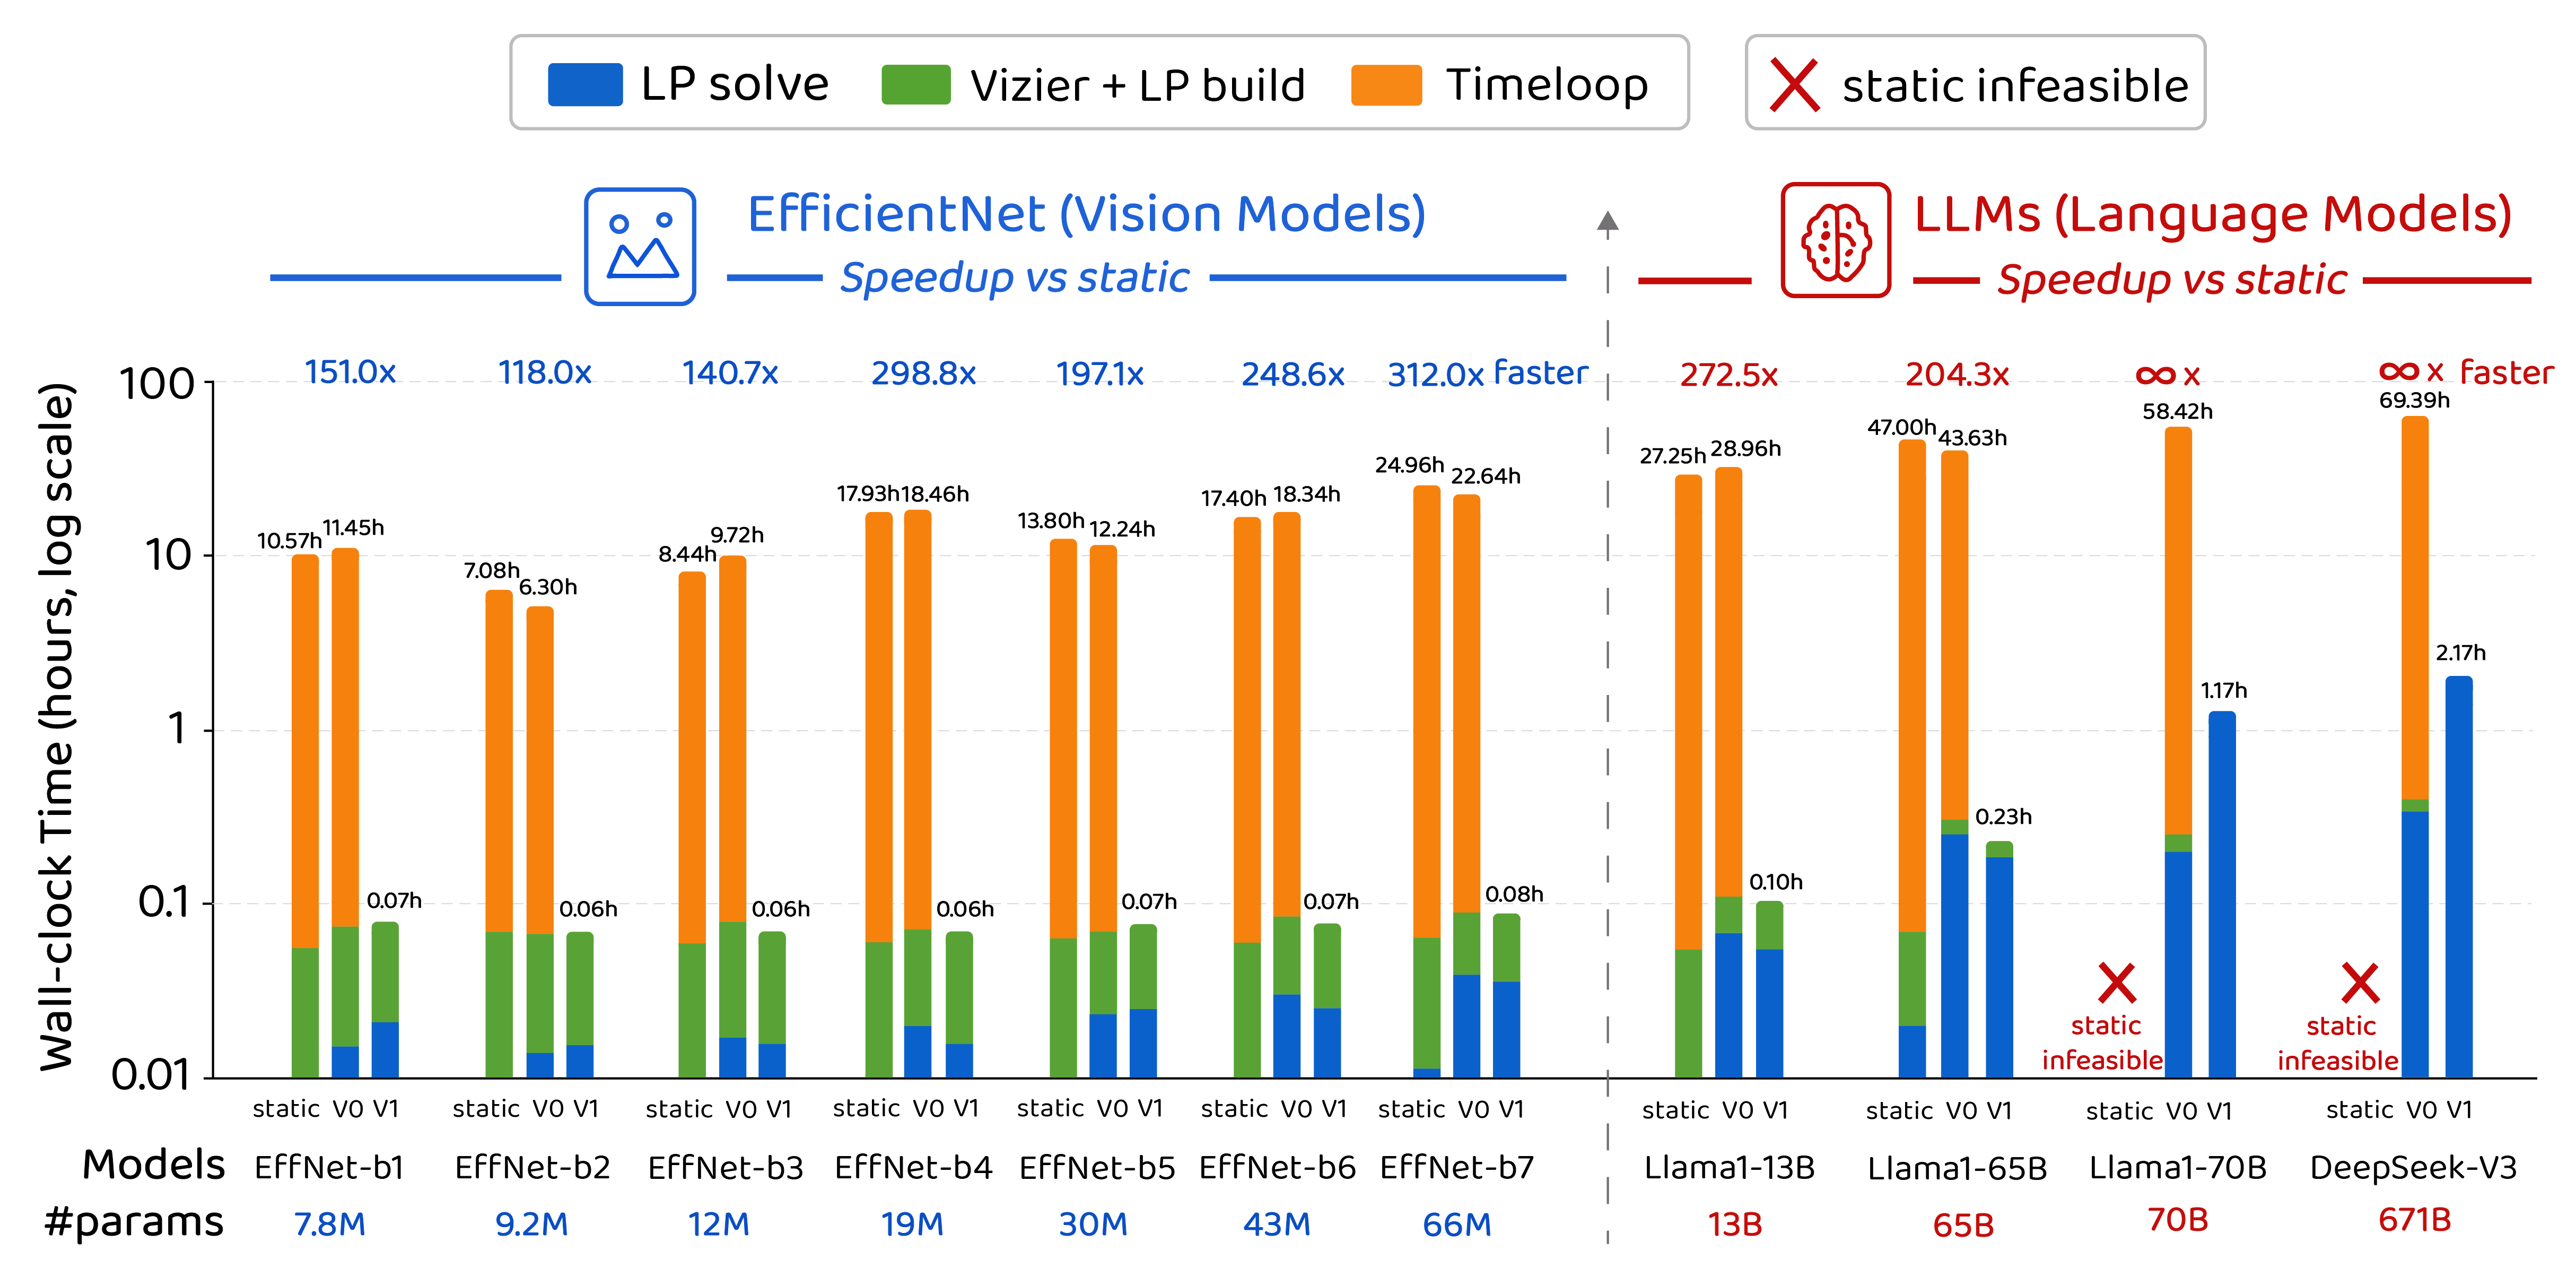
\includegraphics[width=1.0\linewidth]{fig3/wallclock_new_v5.png}
% % % % % \caption{Wall-clock time decomposition and performance acceleration across formulations: CHEETAH-V1's internalized tiling eliminates the Timeloop bottleneck, achieving up to 100–300× faster search than classical static method.}
% % % % % \label{fig:wallclock}
% % % % % \end{figure}

% % % % \begin{figure}[ht!]
% % % %     \centering
% % % % 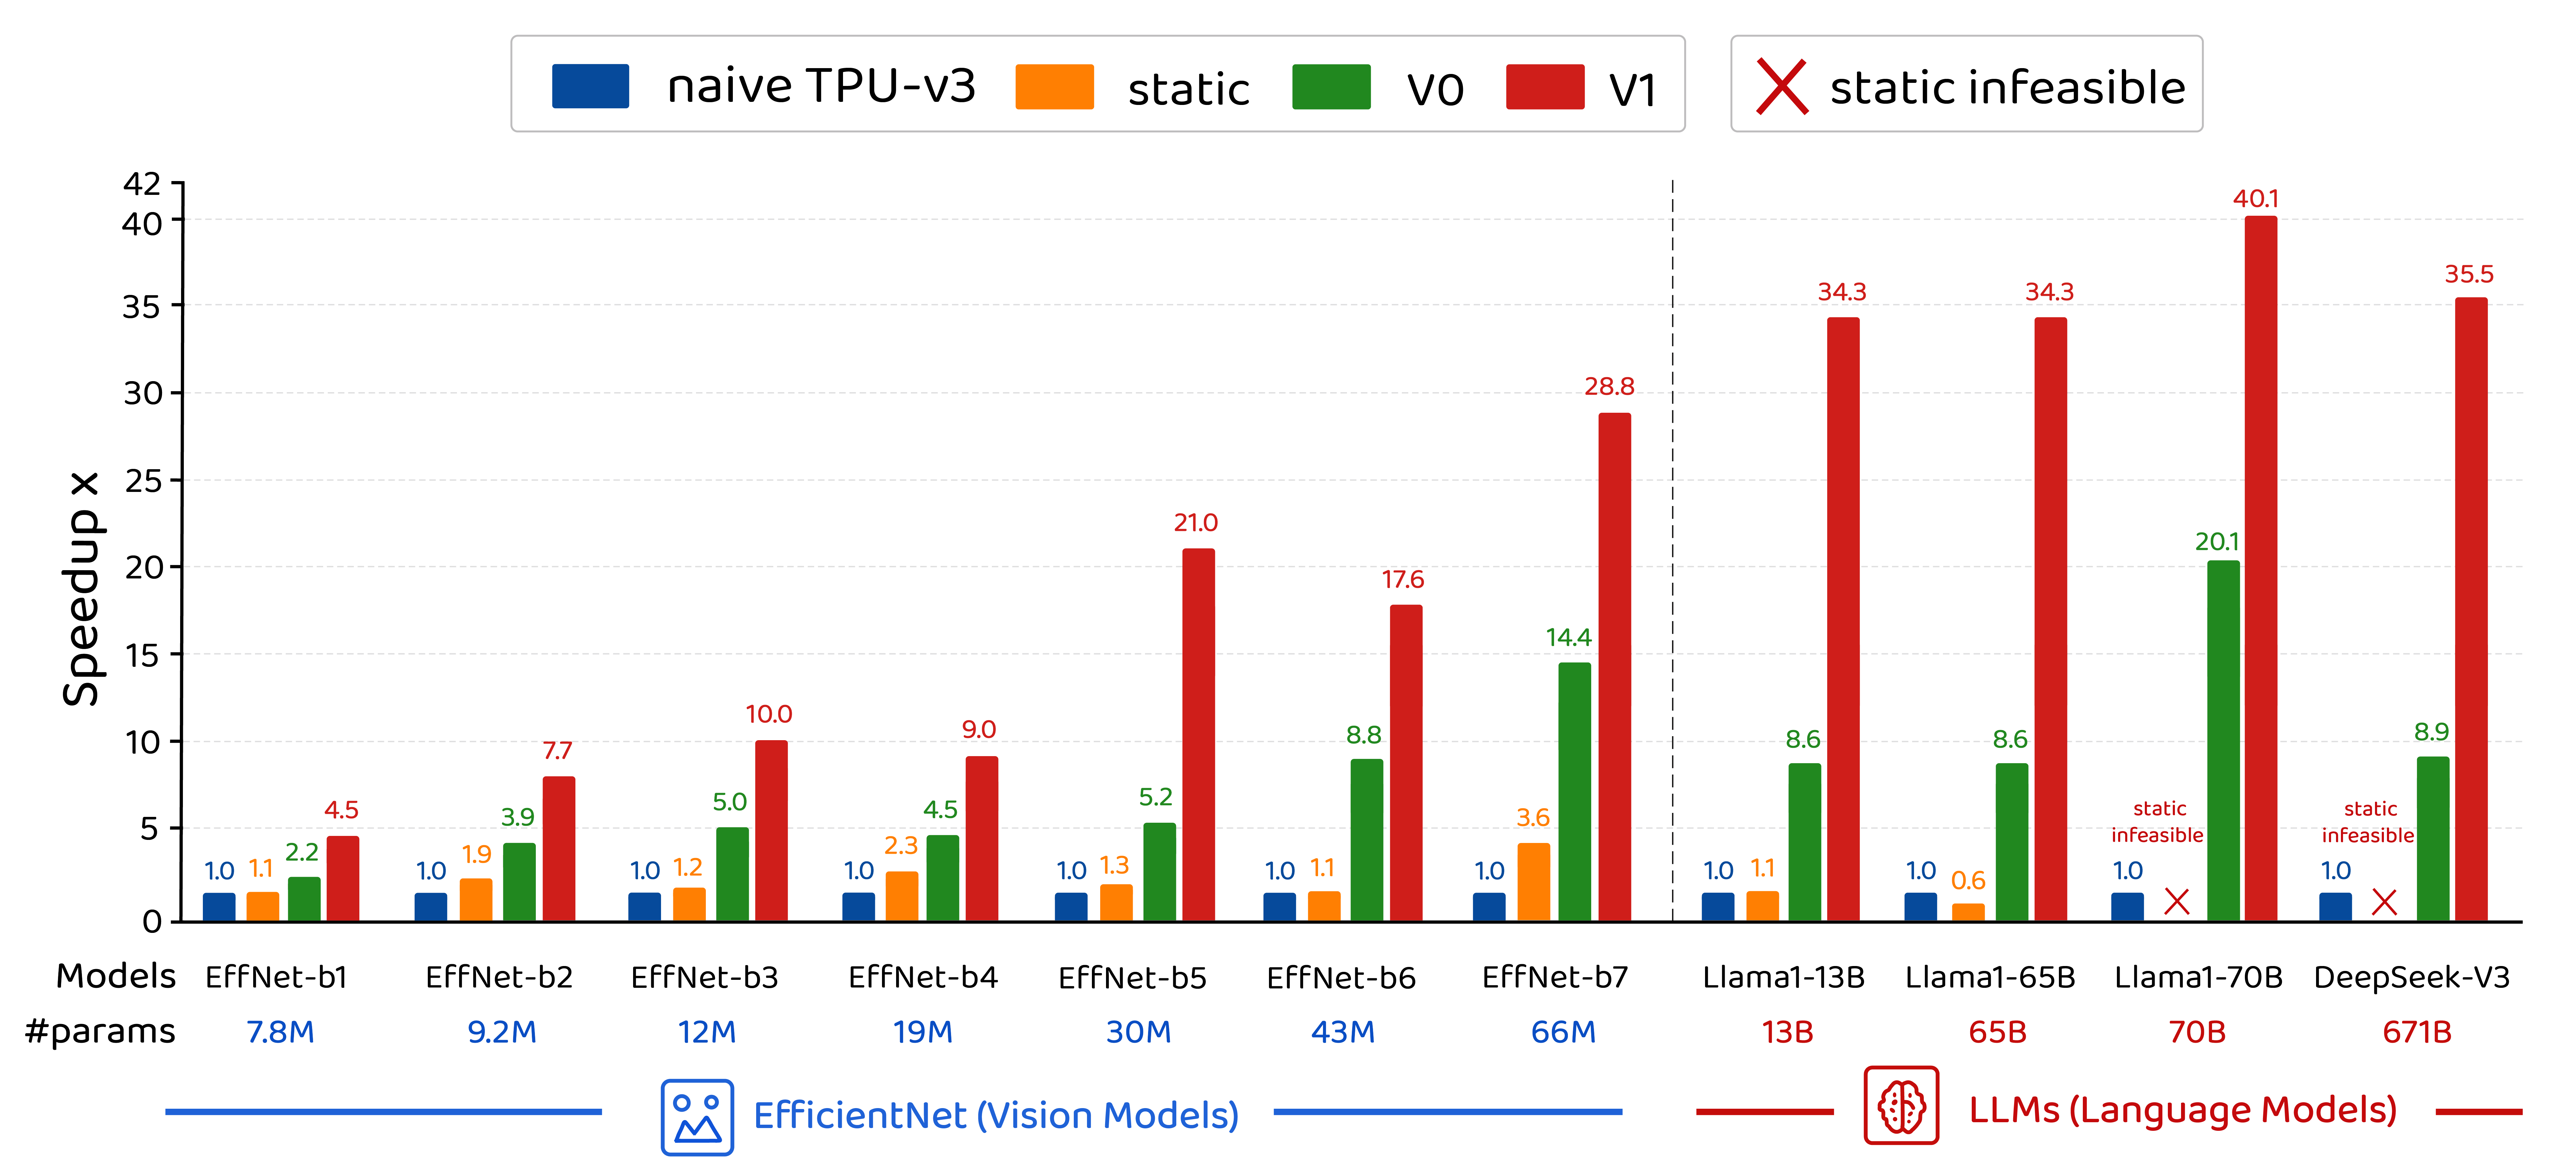
\includegraphics[width=1.0\linewidth]{fig3/speedup_final_v2.png}
% % % % \caption{Speedup over modeled TPU-v3 baseline across formulations and workloads: CHEETAH-V1's joint tiling-fusion optimization achieves up to $\sim$35× acceleration, while static fusion is infeasible on large-scale LLMs.}
% % % % \label{fig:speedup}
% % % % \end{figure}

% % % % % In addition to efficiently enabling more globally optimized accelerator designs, we anticipate that future work may build off this foundation to implement custom Flash Attention type speedup mechanisms for individual hardware (such as RTX5090) and workloads (such as LLama70B) tractably within hours, as well as quickly and efficiently design custom accelerators for targeted inference tasks. 
% % % % % compromise on any single workload; a growing body of evidence suggests that workload-specialized designs can deliver $2$--$6\times$ improvements in performance per watt.
% % % % % The resulting system replaces FAST's sequential Timeloop$\rightarrow$fusion~ILP pipeline with a single LP that jointly optimizes tiling, fusion, and memory scheduling, while preserving Vizier's outer loop over hardware configurations (or replacing it with LLM-guided search).

% % % % % Furthermore, FAST's fusion ILP uses static tensor placement: a tensor is either pinned for the entire inference pass or not at all.
% % % % % This is overly conservative for models with long dependency chains or skip connections, where different tensors are live at different times during execution.
% % % % % A dynamic placement strategy that can evict and re-pin tensors across timesteps could substantially improve global memory utilization. Joint Optimization is the only way to solve the "Memory Wall" for large scale models like DeepSeek-V3.

% % % % % FAST operates via a three-stage sequential pipeline (Figure \ref{fig::workflow}): (1)~a black-box optimizer (Google Vizier \citep{google_vizier}) proposes a hardware configuration defined by 16 hyperparameters---PE grid dimensions, systolic array sizes, buffer capacities, DRAM channels, and batch size; (2)~a scheduling engine (Timeloop \citep{timeloop}) finds the best tiling and mapping for each operation independently given the fixed hardware; and (3)~an integer linear program (ILP) decides which tensors to pin in the on-chip Global Memory to reduce DRAM traffic.
% % % % % The result of each trial---predicted performance per TDP---is fed back to Vizier, which proposes the next hardware configuration, repeating for thousands of trials until convergence.


% % % % % automate the framework with SkyDiscover Loop for profile and context aware co-design. Therefore in less than five hours, we are able to find an more performant design spec than the strongest baseline on designing , in terms of both perf/TDP and speedup. Our experiments also include freezing any hardware at input, and reducing the scheduling, tiling, etc search to just the LP can yield speedups of avg 2.2x than just the base hardware along. We anticipate that future work may build off this foundation to implement custom Flash Attention type speedup mechanisms for individual hardware (such as RTX5090) and workloads (such as LLama70B) tractably within hours. 

% % % % % Our propose the formulation for global co-design for a custom accelerator as a large scale linear program which captures strict dependencies and tradeoffs sequential methods may miss. Our LP formulation captures scheduling, tiling, rematerialization, and is able to solve matrices at scales of $6{,}319 \times 4{,}516$,\ nnz$=829{,}852$ \& $3{,}669{,}793 \times 3{,}263{,}443$,\ nnz$=7{,}342{,}293$ \& $2{,}983{,}450 \times 2{,}504{,}019$,\ nnz$=6{,}094{,}156$ quickly, by utilizing a JAX based large scale solver. Our insight is that despite the challenging large scale of the problem, the structure of the matrices, once formed, retain the same structure. Therefore we are able to design one preconditioning scheme to these large scale systems matrices that can be re-used across any NN. This also allows us to capture dependencies prior methods cannot, for example our formulation introduces a dynamic placement strategy that can evict and re-pin tensors across timesteps could substantially improve global memory utilization. Joint Optimization is the only way to solve the "Memory Wall" for large scale models like DeepSeek-V3. 

% % % % % For EfficientNet-B7 at $L=400$ operations and $T=400$ timesteps, the V1 LP contains approximately $2$ million variables and $5$ million constraints with $15$--$25$ million nonzeros. To better solve such large-scale LP problems more efficiently, we implement our own variant of a GPU-accelerated solver based on recent primal-dual LP algorithm \citep{applegate2022practicallargescalelinearprogramming}. We extend its original formulation in various ways and benchmark our implementation compared to existing commercial SciPy solvers, which showcase the advantage of our solver. To keep the main context clean and focused, we defer LP solver-related details to Appendix \ref{app:solver}.

% % % % % A large number of black box optimization tools to handle this large search space have been recently proposed, such as Google's Vizier, Meta's AX, and Optuna. In addition search strategies are also explored, for example Google's Vizier proposes numerous methods Gaussian Process Upper Confidence Bound, Eagle Strategy as a metaheuristic optimization algorithm designed for global optimization via a two-stage hybrid approach that combines global exploration with intensive local search, and Linear Combination Swarm (LCS). However these methods share certain limitations, since they cannot globally capture the tradeoffs and tensions between sequential decisions and rely on brute force iterations. This requires human engineers to spend months of compute and thousands of repetitive trials to get improvements, without feedback on what might be globally optimal. 

% % % % % While this sequential decomposition makes the problem tractable, it introduces a fundamental limitation: \emph{each stage takes the previous stage's output as fixed input, preventing the discovery of solutions that require trading off across stages.} Consider a concrete example: for a depthwise-separable convolution layer in a NN, a search tool such as Timeloop might select a tiling configuration that maximizes compute utilization at $74\%$, producing an activation working set of $6$ MiB. THe stacked The downstream fusion ILP solver tool receives this fixed working set size, cannot fit the tensor into the $128$ MiB Global Memory alongside other pinned tensors. However, an alternative tiling configuration with slightly lower utilization ($70\%$) might produce a working set of only $3$ MiB, enabling the fusion solver to pin an additional weight tensor that eliminates a DRAM bottleneck entirely, thus yielding a net $>20\%$ cycle reduction despite the $4\%$ utilization loss. Therefore these sequential pipelines systematically misses such cross-stage trade-offs.

% % % % % The rapid evolution of deep learning workloads has created a compelling opportunity for domain-optimized inference accelerators.
% % % % % Production models now serve billions of daily users, and the computational demands of architectures based on depthwise-separable convolutions (EfficientNet), self-attention (BERT, LLaMA), mixture-of-experts (DeepSeek-V3, Mixtral), and state-space models (Mamba) differ dramatically in their compute-to-memory ratios, tensor shapes, and data reuse patterns. However although the NN training strategy has been scaled up and we've done a lot of work on it, we now face the inference bottle neck era since general-purpose hardware, Nvidia's gaming GPUs are not necessarily optimized for deep learning tasks, and leaves a huge amount of compute on the table.


% % % % page edit

% % % \section{Introduction}
% % % \label{sec:introduction}

% % % \begin{figure}[ht!]
% % %     \centering
% % %     \includegraphics[width=1.0\linewidth]{figs/cheetah_v4.png}
% % %     % \caption{\textbf{FAST vs.\ FAST-CORGI pipeline comparison.} 
% % % \caption{Sequential vs Our Unified Optimization Paradigm.
% % % (Left) Baseline methods decouple hardware search, operation-level tiling, and static fusion; precluding cross-stage trade-offs.
% % % (Right) CHEETAH presents a unified LLM-driven LP-solver-based framework that jointly optimizes tiling, placement, and rematerialization while learning from a causal ledger.}
% % % \label{fig::workflow}
% % % \end{figure}
% % % % The rapid evolution of deep learning workloads varies from convolutions to self-attention (LLaMA), mixture-of-experts (DeepSeek-V3), and state-space models (Mamba). These diverse architectures serve billions of daily users, and have fundamentally shifted the requirements for hardware acceleration. As foundation models continue to scale in parameters, the primary cost and bottleneck of model deployment has shifted from training to inference. Therefore much recent research has been focused on optimizing for more efficient execution and throughput across diverse, high-dimensional workloads. General-purpose GPUs remain largely designed for graphics-heavy throughput, and leave substantial efficiency and compute on the table at these tasks. Therefore we are motivated to design targeted accelerators that are optimized for handling the varying tensor shapes and data-reuse patterns of modern deep learning architectures.
% % % % Much research has been done in accelerating inference through custom accelerator design, more efficient neural network (NN) batching algorithms, and domain specific packages and languages that aim to speed up general NN inference. For example, the widely adopted Flash Attention uses tiling to provide significant speedups by optimizing memory movement between SRAM and DRAM. Co-design takes this a step further by aiming to optimize hardware, software and scheduling to unlock performance neither could reach independently. The traditional framework of doing this is a sequential pipeline of heuristics tools, requiring human engineers to iterate through a large search space for months from testing for the size of DRAM, to determining higher level scheduling problems. Optimizing each piece of this complex pipeline is extremely challenging, since hardware datapaths, software schedules, and compiler transforms across a combinatorial space exceeding $\mathcal O(10^{2300})$.
% % % The AI inference demand is expected to grow by $10,000\times$ over the next 5 years \citep{cra2026aifuture}. General-purpose accelerators leave significant efficiency gains unrealized, which motivates the design of targeted custom accelerators. Co-design, which jointly optimizes hardware-software (HW/SW), and scheduling for target workloads, offers a path to unlock performance efficiency for the upcoming inference era. However, the prevailing approach relies on sequential pipelines of heuristic tools, a slow, human-driven process navigating a combinatorial search space exceeding $O(10^{2300})$ \citep{zhang_fast}. State-of-the-art frameworks like FAST \citep{zhang_fast} improve on through an automated flow (a hardware proposer feeds an operation-level tiling agent, which feeds a downstream fusion solver), but remain fundamentally decoupled.  For example, a tiling configuration that is \textit{locally} optimal for one layer may create an activation footprint that later prevents \textit{global} fusion, while a slightly slower tiling might shrink the working set enough to eliminate a DRAM bottleneck entirely. Sequential pipelines are systematically unable to express these interactions, leading to locally good but globally sub-optimal designs.

% % % % The co-design problem is increasingly important as inference efficiency is the dominant AI workload and is rapidly growing. Therefore industry leaders such as NVIDIA and Google have designed chips for improved hardware-native agentic AI and , and state-of-the-art frameworks such as FAST, address this through a sequential decomposition of heuristics (a hardware proposer feeds an operation-level tiling agent, which feeds a downstream fusion solver). While FAST-generated accelerators can provide increased speedups over baseline TPU-v3, this decoupled approach is limited since it cannot capture cross-stage trade-offs. A tiling configuration that is \textit{locally} optimal for one layer may create an activation footprint that later prevents \textit{global} fusion, while a slightly slower tiling might shrink the working set enough to eliminate a DRAM bottleneck entirely. Sequential pipelines are systematically unable to express these interactions, leading to locally good but globally sub-optimal designs. 
% % % We prove that by unifying the design space into a single convex relaxation, we find global optima that were previously  infeasible. Specifically, we introduce CHEETAH: a custom inference accelerator design framework that unlocks globally optimized designs with a dual-loop. Our inner-loop is a novel large-scale Linear Program (LP) to precisely mathematically model strict design decisions and constraints that must not be violated. The LP captures trade-offs for targeted workloads through time-indexed placement and rematerialization, thus allowing tensors to be dynamically pinned, evicted, recomputed across inference timesteps. We further extend our reformulation to internalize tiling selection into the LP, by introducing Pareto-pruned tiling variables and the McCormick linearization (a convex relaxation used for optimization of bilinear problems \citep{mccormick1976computability}). By exploiting the structural invariance of our matrices across hardware trials, we also adapt a GPU-accelerated primal-dual solver in JAX \citep{jax2018github} that can resolve millions of variables to rapidly reduce trial time from days to hours. This allows the LP solver to jointly reason about hardware configuration, activation placement, and weight pinning in a single pass, while providing feedback signal via Lagrangian duals.

% % % Our outer-loop framework stacks a black-box optimizer (Google Vizier \citep{google_vizier}) to propose candidate hardware configurations defined by a set of hyperparameters (e.g., processing element grid dimensions, systolic array sizes, DRAM size, etc), while a LLM is used for efficient search-space steering. The LLM acts as a causal architect, interpreting a compact trial ledger of roofline checks and LP feedback diagnostics to propose constrained architectural search input for Vizier. This prevents the search-space gaming typical of black-box optimizers in wide design regions, and reduces the need for thousands of sequential trials via Bayesian search strategies in Vizier to learn good vs bad neighborhoods in search topology. Our results demonstrate that the LLM Architect framework further reduces invalid hardware trials from 24.5\% under vanilla Vizier to 5.9\%, while reaching the Pareto frontier 4.5x faster than the next strongest baseline. We validate all results with Model Flop Utilization (MFU) and roofline lower-bound audits, ensuring predicted latencies are physically grounded in compute and memory throughput limits. 
% % % % \todo{Add best of both worlds, strengths from principled LP side, from LLM aggregate info side}
% % % % \todo{Aggregates past experience to gain insight into steering hardware-software co-design. We offload the strict solves, with constraints that must the strictly respected, to the LP solve part. This combines the best of both worlds.} 
% % % \paragraph{Contributions.} We reformulated the fundamental HW/SW co-design problem into a unified  framework in CHEETAH, combining principled mathematical rigor of the LP formulation to solve strict design decisions optimally, with the powerful aggregation and causal learning of an LLM Architect outer loop for meta-optimization. Our open-source repository for full reproducibility is at \href{https://anonymous.4open.science/r/CHEETAH-B268/readme}{https://anonymous.4open.science/r/CHEETAH-B268/}.

% % % \begin{enumerate}
% % %     \item \textbf{CHEETAH-V0 - Dynamic Placement with Rematerialization:}
% % %     We introduce time-indexed LP variables $p_{i,t}^k$ and rematerialization variables $r_{i,t}$ to enable cheap recompute operations (\eg, depthwise convolutions that account for only $5\%$ of FLOPs but produce large activations) instead of paying DRAM reload costs, supporting skip connections and multi-fanout nodes.

% % %     \item \textbf{CHEETAH-V1 - Joint Tiling-Fusion:}
% % %     We unify tiling and fusion into a single LP problem by introducing tiling selection variables $y_{i,c}$, and employ McCormick envelopes to exactly linearize the bilinear interaction between tiling and tensor pinning. This technique yields a tight, parameter-free LP relaxation, and the coupling internalizes the tiling-placement trade-off to discover optimal design points that sequential pipelines systematically miss.
% % %     % This enables the LP to discover trade-offs where accepting a suboptimal tiling configuration enables superior fusion, or vice versa---precisely the cross-stage interactions that the sequential pipeline cannot capture.
% % %     \item \textbf{LLM-guided Causal Architect:} The LLM outer loop steers hardware search by interpreting Lagrangian sensitivity signals and a Causal Ledger of past trials to perform targeted subspace interventions, transforming black-box search into a structured, diagnostic-driven process. The Architect guides Vizier through widened search spaces, reducing invalid trials by ${\sim}4\times$ while preserving the global optimal score, and enables profile-specific designs (speech models may emphasize latency, while data synthesis models may prioritize bandwidth). 
% % %     \item \textbf{Speedup:} Our method demonstrates an average speedup of $\sim22.07\times$ over the baseline across a wide range of $11$ vision and language models. 

% % %     % profiles into consideration to push the black-box optimizer responsible for hardware suggestions to output with structured reasoning about architectural trade-offs. 

% % % \end{enumerate}

% % % \begin{figure}[ht!]
% % %     \centering
% % % 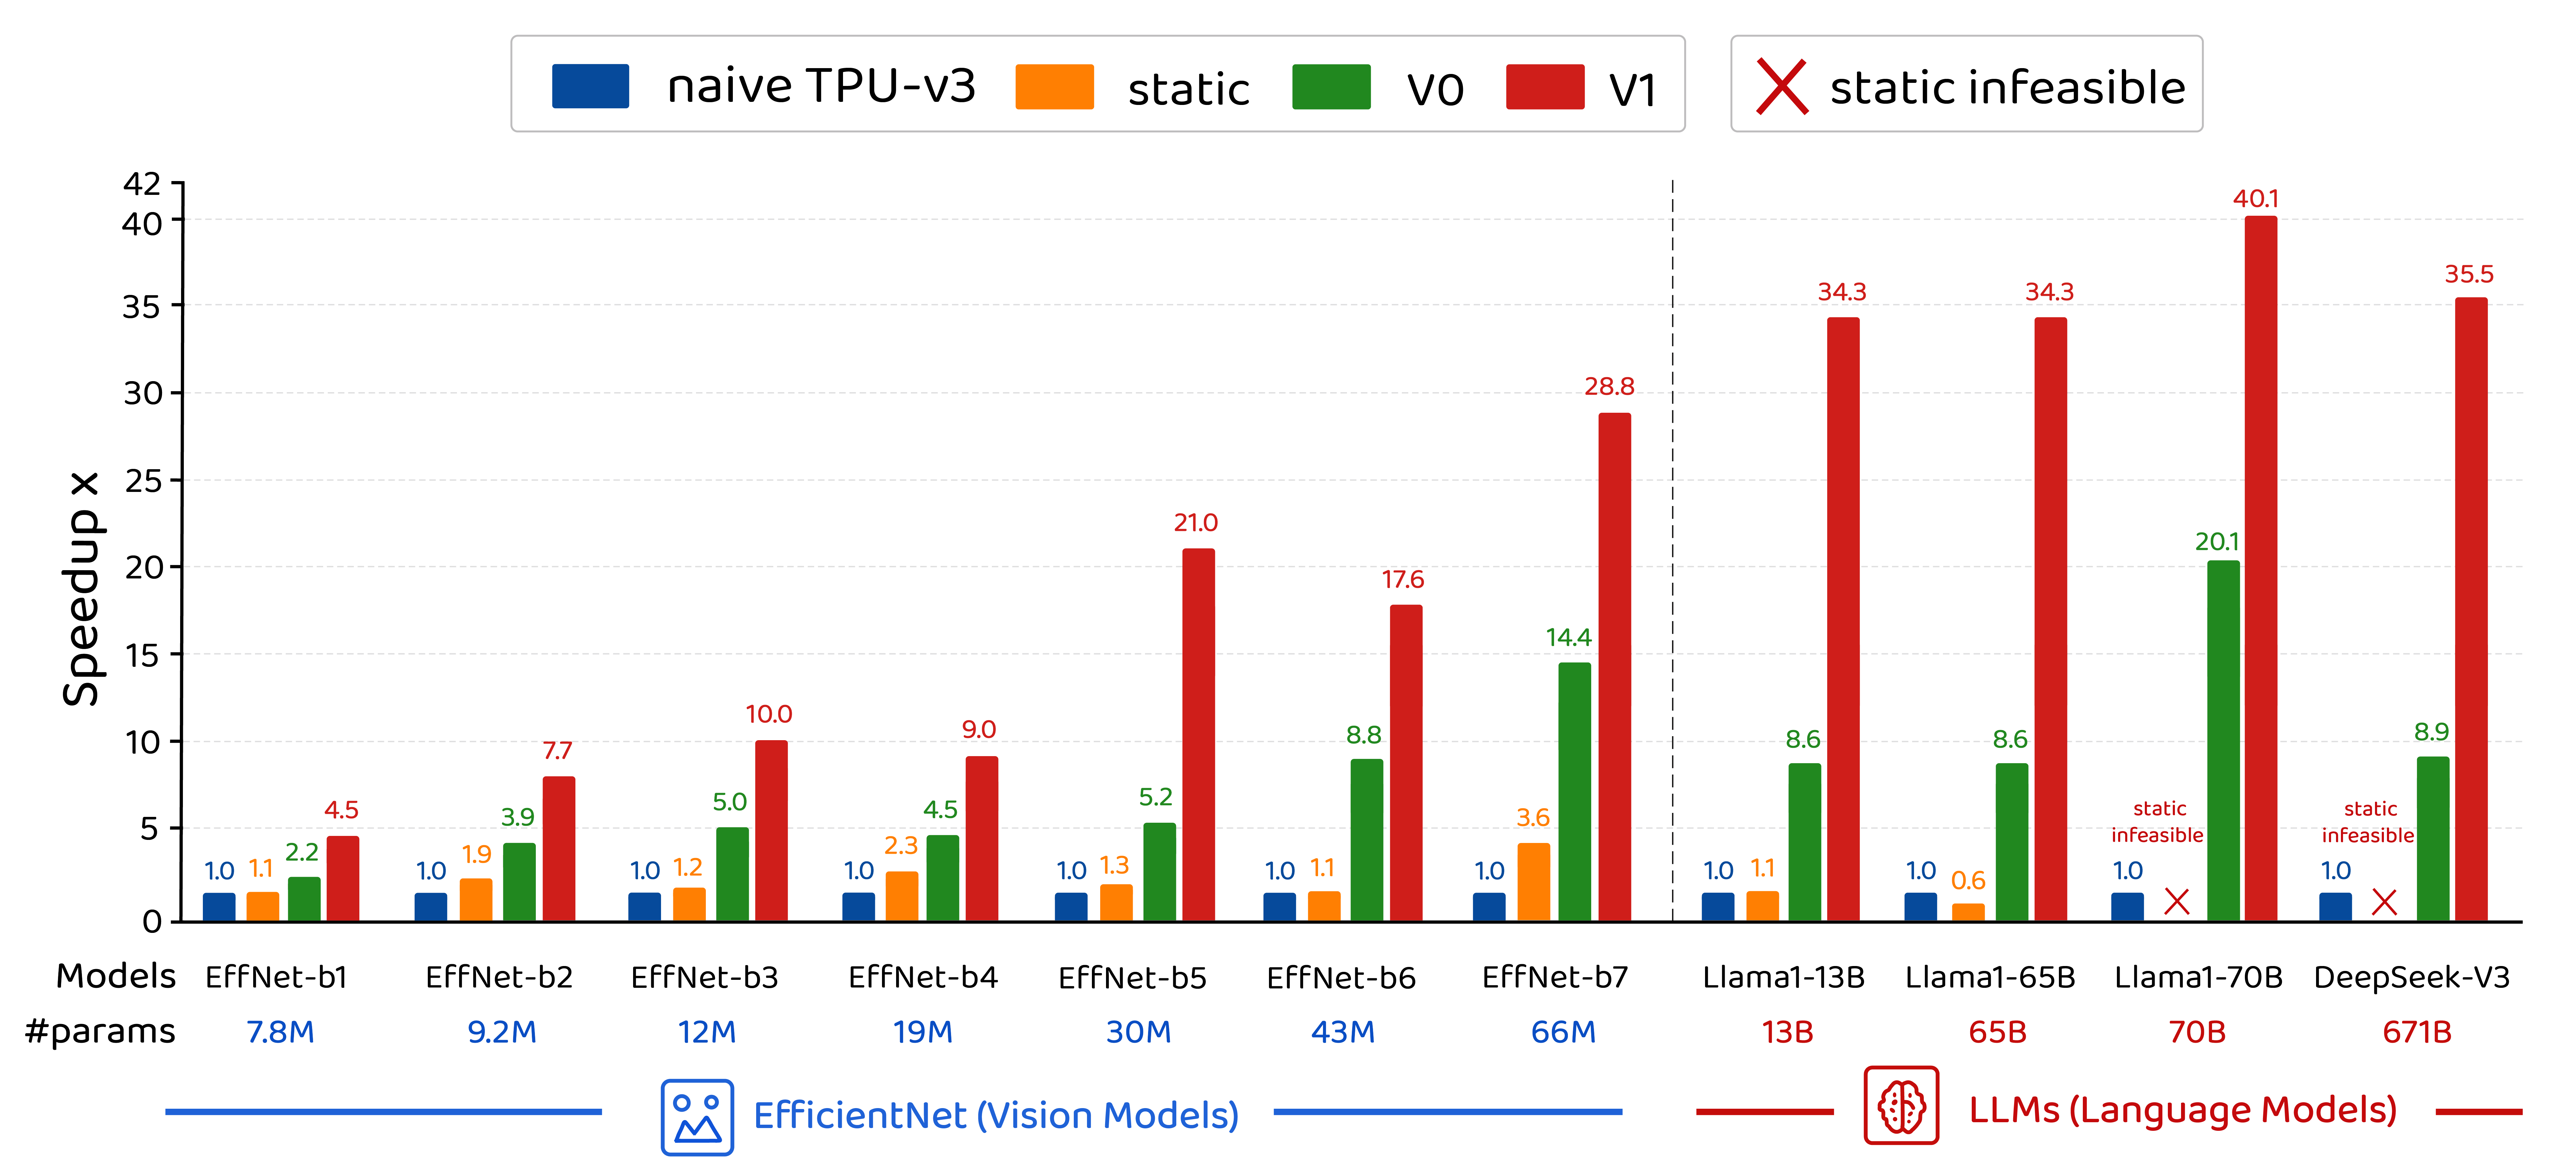
\includegraphics[width=1.0\linewidth]{fig3/speedup_final_v2.png}
% % % \caption{Speedup over modeled TPU-v3 baseline across formulations and workloads: CHEETAH-V1's joint tiling-fusion optimization achieves up to $\sim$40.1$\times$ acceleration, while static fusion is infeasible on large-scale LLMs. Progressive gains are visible across formulations: V0's dynamic placement improves over static by $2$--$20\times$, while V1's joint tiling-fusion adds another $2$--$4\times$ on top. See Section~\ref{sec:experiments} for full analysis and wall-clock time breakdowns.}
% % % \label{fig:speedup}
% % % \end{figure}

% % % % In addition to efficiently enabling more globally optimized accelerator designs, we anticipate that future work may build off this foundation to implement custom Flash Attention type speedup mechanisms for individual hardware (such as RTX5090) and workloads (such as LLama70B) tractably within hours, as well as quickly and efficiently design custom accelerators for targeted inference tasks. 
% % % % compromise on any single workload; a growing body of evidence suggests that workload-specialized designs can deliver $2$--$6\times$ improvements in performance per watt.
% % % % The resulting system replaces FAST's sequential Timeloop$\rightarrow$fusion~ILP pipeline with a single LP that jointly optimizes tiling, fusion, and memory scheduling, while preserving Vizier's outer loop over hardware configurations (or replacing it with LLM-guided search).

% % % % Furthermore, FAST's fusion ILP uses static tensor placement: a tensor is either pinned for the entire inference pass or not at all.
% % % % This is overly conservative for models with long dependency chains or skip connections, where different tensors are live at different times during execution.
% % % % A dynamic placement strategy that can evict and re-pin tensors across timesteps could substantially improve global memory utilization. Joint Optimization is the only way to solve the "Memory Wall" for large scale models like DeepSeek-V3.

% % % % FAST operates via a three-stage sequential pipeline (Figure \ref{fig::workflow}): (1)~a black-box optimizer (Google Vizier \citep{google_vizier}) proposes a hardware configuration defined by 16 hyperparameters---PE grid dimensions, systolic array sizes, buffer capacities, DRAM channels, and batch size; (2)~a scheduling engine (Timeloop \citep{timeloop}) finds the best tiling and mapping for each operation independently given the fixed hardware; and (3)~an integer linear program (ILP) decides which tensors to pin in the on-chip Global Memory to reduce DRAM traffic.
% % % % The result of each trial---predicted performance per TDP---is fed back to Vizier, which proposes the next hardware configuration, repeating for thousands of trials until convergence.


% % % % automate the framework with SkyDiscover Loop for profile and context aware co-design. Therefore in less than five hours, we are able to find an more performant design spec than the strongest baseline on designing , in terms of both perf/TDP and speedup. Our experiments also include freezing any hardware at input, and reducing the scheduling, tiling, etc search to just the LP can yield speedups of avg 2.2x than just the base hardware along. We anticipate that future work may build off this foundation to implement custom Flash Attention type speedup mechanisms for individual hardware (such as RTX5090) and workloads (such as LLama70B) tractably within hours. 

% % % % Our propose the formulation for global co-design for a custom accelerator as a large scale linear program which captures strict dependencies and tradeoffs sequential methods may miss. Our LP formulation captures scheduling, tiling, rematerialization, and is able to solve matrices at scales of $6{,}319 \times 4{,}516$,\ nnz$=829{,}852$ \& $3{,}669{,}793 \times 3{,}263{,}443$,\ nnz$=7{,}342{,}293$ \& $2{,}983{,}450 \times 2{,}504{,}019$,\ nnz$=6{,}094{,}156$ quickly, by utilizing a JAX based large scale solver. Our insight is that despite the challenging large scale of the problem, the structure of the matrices, once formed, retain the same structure. Therefore we are able to design one preconditioning scheme to these large scale systems matrices that can be re-used across any NN. This also allows us to capture dependencies prior methods cannot, for example our formulation introduces a dynamic placement strategy that can evict and re-pin tensors across timesteps could substantially improve global memory utilization. Joint Optimization is the only way to solve the "Memory Wall" for large scale models like DeepSeek-V3. 

% % % % For EfficientNet-B7 at $L=400$ operations and $T=400$ timesteps, the V1 LP contains approximately $2$ million variables and $5$ million constraints with $15$--$25$ million nonzeros. To better solve such large-scale LP problems more efficiently, we implement our own variant of a GPU-accelerated solver based on recent primal-dual LP algorithm \citep{applegate2022practicallargescalelinearprogramming}. We extend its original formulation in various ways and benchmark our implementation compared to existing commercial SciPy solvers, which showcase the advantage of our solver. To keep the main context clean and focused, we defer LP solver-related details to Appendix \ref{app:solver}.

% % % % A large number of black box optimization tools to handle this large search space have been recently proposed, such as Google's Vizier, Meta's AX, and Optuna. In addition search strategies are also explored, for example Google's Vizier proposes numerous methods Gaussian Process Upper Confidence Bound, Eagle Strategy as a metaheuristic optimization algorithm designed for global optimization via a two-stage hybrid approach that combines global exploration with intensive local search, and Linear Combination Swarm (LCS). However these methods share certain limitations, since they cannot globally capture the tradeoffs and tensions between sequential decisions and rely on brute force iterations. This requires human engineers to spend months of compute and thousands of repetitive trials to get improvements, without feedback on what might be globally optimal. 

% % % % While this sequential decomposition makes the problem tractable, it introduces a fundamental limitation: \emph{each stage takes the previous stage's output as fixed input, preventing the discovery of solutions that require trading off across stages.} Consider a concrete example: for a depthwise-separable convolution layer in a NN, a search tool such as Timeloop might select a tiling configuration that maximizes compute utilization at $74\%$, producing an activation working set of $6$ MiB. THe stacked The downstream fusion ILP solver tool receives this fixed working set size, cannot fit the tensor into the $128$ MiB Global Memory alongside other pinned tensors. However, an alternative tiling configuration with slightly lower utilization ($70\%$) might produce a working set of only $3$ MiB, enabling the fusion solver to pin an additional weight tensor that eliminates a DRAM bottleneck entirely, thus yielding a net $>20\%$ cycle reduction despite the $4\%$ utilization loss. Therefore these sequential pipelines systematically misses such cross-stage trade-offs.

% % % % The rapid evolution of deep learning workloads has created a compelling opportunity for domain-optimized inference accelerators.
% % % % Production models now serve billions of daily users, and the computational demands of architectures based on depthwise-separable convolutions (EfficientNet), self-attention (BERT, LLaMA), mixture-of-experts (DeepSeek-V3, Mixtral), and state-space models (Mamba) differ dramatically in their compute-to-memory ratios, tensor shapes, and data reuse patterns. However although the NN training strategy has been scaled up and we've done a lot of work on it, we now face the inference bottle neck era since general-purpose hardware, Nvidia's gaming GPUs are not necessarily optimized for deep learning tasks, and leaves a huge amount of compute on the table.


% % % page limit edit

% % % \section{Introduction}
% % % \label{sec:introduction}

% % % \begin{figure}[ht!]
% % %     \centering
% % %     \includegraphics[width=1.0\linewidth]{figs/cheetah_v4.png}
% % % \caption{Sequential vs Unified Optimization Paradigm Comparison.
% % % (Left) Baseline methods decouple hardware search, operation-level tiling, and static fusion; precluding cross-stage trade-offs.
% % % (Right) CHEETAH presents a unified LLM-driven LP-solver-based framework that jointly optimizes tiling, placement, and rematerialization while learning from a causal ledger.}
% % % \label{fig::workflow}
% % % \end{figure}
% % % % The rapid evolution of deep learning workloads varies from convolutions to self-attention (LLaMA), mixture-of-experts (DeepSeek-V3), and state-space models (Mamba). These diverse architectures serve billions of daily users, and have fundamentally shifted the requirements for hardware acceleration. As foundation models continue to scale in parameters, the primary cost and bottleneck of model deployment has shifted from training to inference. Therefore much recent research has been focused on optimizing for more efficient execution and throughput across diverse, high-dimensional workloads. General-purpose GPUs remain largely designed for graphics-heavy throughput, and leave substantial efficiency and compute on the table at these tasks. Therefore we are motivated to design targeted accelerators that are optimized for handling the varying tensor shapes and data-reuse patterns of modern deep learning architectures.
% % % % Much research has been done in accelerating inference through custom accelerator design, more efficient neural network (NN) batching algorithms, and domain specific packages and languages that aim to speed up general NN inference. For example, the widely adopted Flash Attention uses tiling to provide significant speedups by optimizing memory movement between SRAM and DRAM. Co-design takes this a step further by aiming to optimize hardware, software and scheduling to unlock performance neither could reach independently. The traditional framework of doing this is a sequential pipeline of heuristics tools, requiring human engineers to iterate through a large search space for months from testing for the size of DRAM, to determining higher level scheduling problems. Optimizing each piece of this complex pipeline is extremely challenging, since hardware datapaths, software schedules, and compiler transforms across a combinatorial space exceeding $\mathcal O(10^{2300})$.
% % % The AI inference demand is expected to grow by $10,000\times$ over the next 5 years \citep{cra2026aifuture}. General-purpose accelerators leave significant efficiency gains unrealized, which motivates the design of targeted custom accelerators. Co-design, which jointly optimizes hardware, software, and scheduling for target workloads, offers a path to unlock performance efficiency for the upcoming inference era. However, the prevailing approach relies on sequential pipelines of heuristic tools, a slow, human-driven process navigating a combinatorial search space exceeding $O(10^{2300})$ \citep{zhang_fast}. State-of-the-art frameworks like FAST \citep{zhang_fast} improve on through an automated flow (a hardware proposer feeds an operation-level tiling agent, which feeds a downstream fusion solver), but remain fundamentally decoupled.  For example, a tiling configuration that is \textit{locally} optimal for one layer may create an activation footprint that later prevents \textit{global} fusion, while a slightly slower tiling might shrink the working set enough to eliminate a DRAM bottleneck entirely. Sequential pipelines are systematically unable to express these interactions, leading to locally good but globally sub-optimal designs.

% % % % The co-design problem is increasingly important as inference efficiency is the dominant AI workload and is rapidly growing. Therefore industry leaders such as NVIDIA and Google have designed chips for improved hardware-native agentic AI and , and state-of-the-art frameworks such as FAST, address this through a sequential decomposition of heuristics (a hardware proposer feeds an operation-level tiling agent, which feeds a downstream fusion solver). While FAST-generated accelerators can provide increased speedups over baseline TPU-v3, this decoupled approach is limited since it cannot capture cross-stage trade-offs. A tiling configuration that is \textit{locally} optimal for one layer may create an activation footprint that later prevents \textit{global} fusion, while a slightly slower tiling might shrink the working set enough to eliminate a DRAM bottleneck entirely. Sequential pipelines are systematically unable to express these interactions, leading to locally good but globally sub-optimal designs. 
% % % We prove that by unifying the design space into a single convex relaxation, we find global optima that were previously  infeasible. Specifically, we introduce CHEETAH: a custom inference accelerator design framework that unlocks globally optimized designs with a dual-loop engine (See Figure \ref{fig::workflow}). Our inner-loop is a novel large-scale Linear Program (LP) to precisely mathematically model strict design decisions and constraints that must not be violated. The LP captures trade-offs for targeted workloads through time-indexed placement and rematerialization, thus allowing tensors to be dynamically pinned, evicted, recomputed across inference timesteps. We further extend our reformulation to internalize tiling selection into the LP, by introducing Pareto-pruned tiling variables and the McCormick linearization (a convex relaxation used for optimization of bilinear problems \citep{mccormick1976computability}). By exploiting the structural invariance of our matrices across hardware trials, we also adapt a GPU-accelerated primal-dual solver in JAX that can resolve millions of variables to rapidly reduce trial time from days to hours. This allows the LP solver to jointly reason about hardware configuration, activation placement, and weight pinning in a single pass, while providing feedback signal via Lagrangian duals.

% % % Our outer-loop framework stacks a black-box optimizer (Google Vizier \citep{google_vizier}) to propose candidate hardware configurations defined by a set of hyperparameters (e.g., processing element grid dimensions, systolic array sizes, DRAM size, etc), while a LLM is used for efficient search-space steering. The LLM acts as a causal architect, interpreting a compact trial ledger of roofline checks and LP feedback diagnostics to propose constrained architectural search input for Vizier. This prevents the search-space gaming typical of black-box optimizers in wide design regions, and reduces the need for thousands of sequential trails via Bayesian search strategies in Vizier to learn good vs bad neighborhoods in search topology. Our results demonstrate that the LLM-Architect framework further reduces invalid hardware trials from 24.5\% under vanilla Vizier to 5.9\%, while reaching the Pareto frontier 4.5x faster than the next strongest baseline. We validate all results with Model Flop Utilization (MFU)  and roofline lower-bound audits, ensuring predicted latencies are physically grounded in compute and memory throughput limits. 
% % % % \todo{Add best of both worlds, strengths from principled LP side, from LLM aggregate info side}
% % % % \todo{Aggregates past experience to gain insight into steering hardware-software co-design. We offload the strict solves, with constraints that must the strictly respected, to the LP solve part. This combines the best of both worlds.} 
% % % \paragraph{Contributions.} We reformulated the fundamental HW/SW co-design problem into a unified  framework in CHEETAH, combining principled mathematical rigor of the LP formulation to solve strict design decisions optimally, with the powerful aggregation and causal learning of an LLM Architect outer loop for meta-optimization. Our open-source repository for full reproducibility is at \href{https://anonymous.4open.science/r/CHEETAH-B268/readme}{https://anonymous.4open.science/r/CHEETAH-B268/}.

% % % \begin{enumerate}
% % %     \item \textbf{CHEETAH-V0 - Dynamic Placement with Rematerialization:}
% % %     We introduce the time-indexed and rematerialization variables to enable cheap recompute operations (\eg, depthwise convolutions that account for only $5\%$ of FLOPs but produce large activations) instead of paying DRAM reload costs. This addresses the restrictions of existing baseline methods where activations can only be pinned between consecutively-executed operations, and supports skip connections and multi-fanout nodes.

% % %     \item \textbf{CHEETAH-V1 - Joint Tiling-Fusion:}
% % %     We unify tiling and fusion into a single LP problem by introducing tiling selection variables $y_{i,c}$, and employ McCormick envelopes to exactly linearize the bilinear interaction between tiling and tensor pinning. This technique yields a tight, parameter-free LP relaxation, and the coupling internalizes the tiling-placement trade-off to discover optimal design points that sequential pipelines systematically miss.
% % %     % This enables the LP to discover trade-offs where accepting a suboptimal tiling configuration enables superior fusion, or vice versa---precisely the cross-stage interactions that the sequential pipeline cannot capture.
% % %     \item \textbf{LLM-guided Causal Architect:} The LLM outer loop steers hardware search and bridges high-level architectural reasoning with low-level solver duals. It interprets Lagrangian sensitivity signals to perform targeted subspace interventions, transforming black-box search into a structured, diagnostic-driven process. We use a context-aware LLM Architect to propose good search areas as input to Vizier (a black-box Bayesian optimizer). Feedback signals are aggregated across historical trials through both the Causal Ledger and the LP solver. The Architect then guides Vizier through widened search spaces, reducing invalid trials by ${\sim}4\times$ while preserving the global optimal score, while enabling profile-specific designs (speech models may emphasize latency, while data synthesis models may prioritize bandwidth). 
% % %     \item \textbf{Speedup:} We show that across a large suite of vision and language modeling workloads, CHEETAH results in an average of 20.9X faster designs than prior work. 

% % %     % profiles into consideration to push the black-box optimizer responsible for hardware suggestions to output with structured reasoning about architectural trade-offs. 

% % % \end{enumerate}

% % % We anticipate that future work may build from this framework in two ways: as an end-to-end co-design system for efficient accelerators, and as an automated optimization engine for existing hardware. By fixing the architecture, the inner loop derives optimal tiling and scheduling strategies that can act as custom speedups for targeted inference tasks.

% % % % \begin{figure}[ht!] 
% % % %     \centering
% % % % 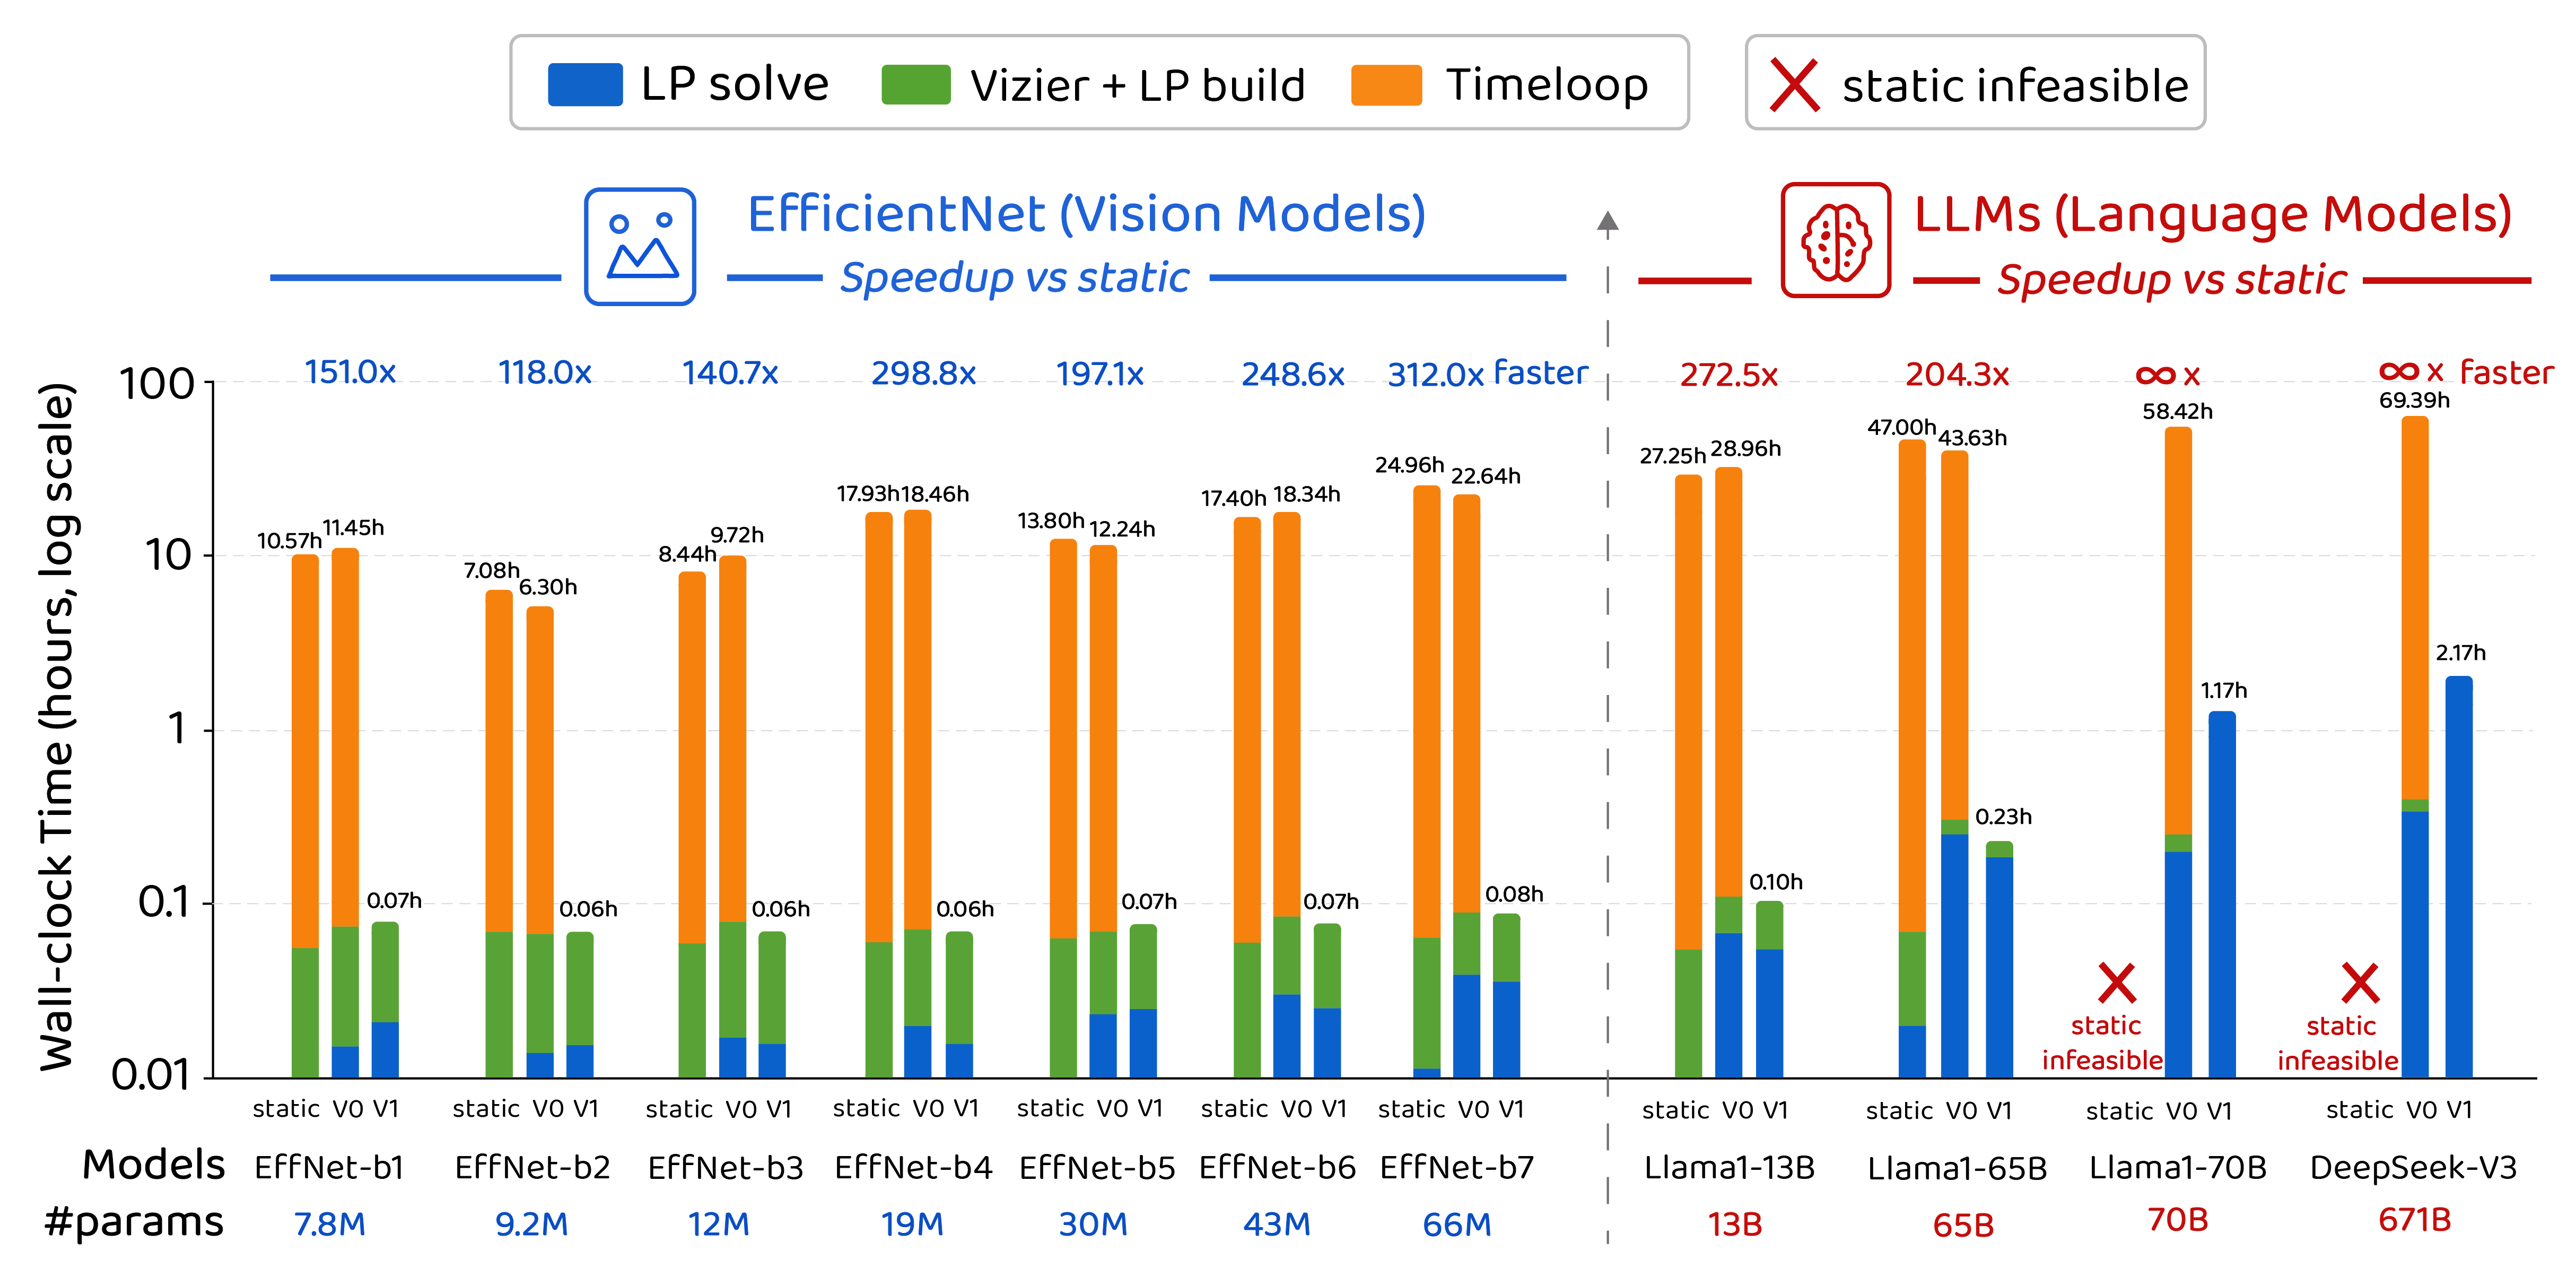
\includegraphics[width=1.0\linewidth]{fig3/wallclock_new_v5.png}
% % % % \caption{Wall-clock time decomposition and performance acceleration across formulations: CHEETAH-V1's internalized tiling eliminates the Timeloop bottleneck, achieving up to 100–300× faster search than classical static method.}
% % % % \label{fig:wallclock}
% % % % \end{figure}

% % % \begin{figure}[ht!]
% % %     \centering
% % % 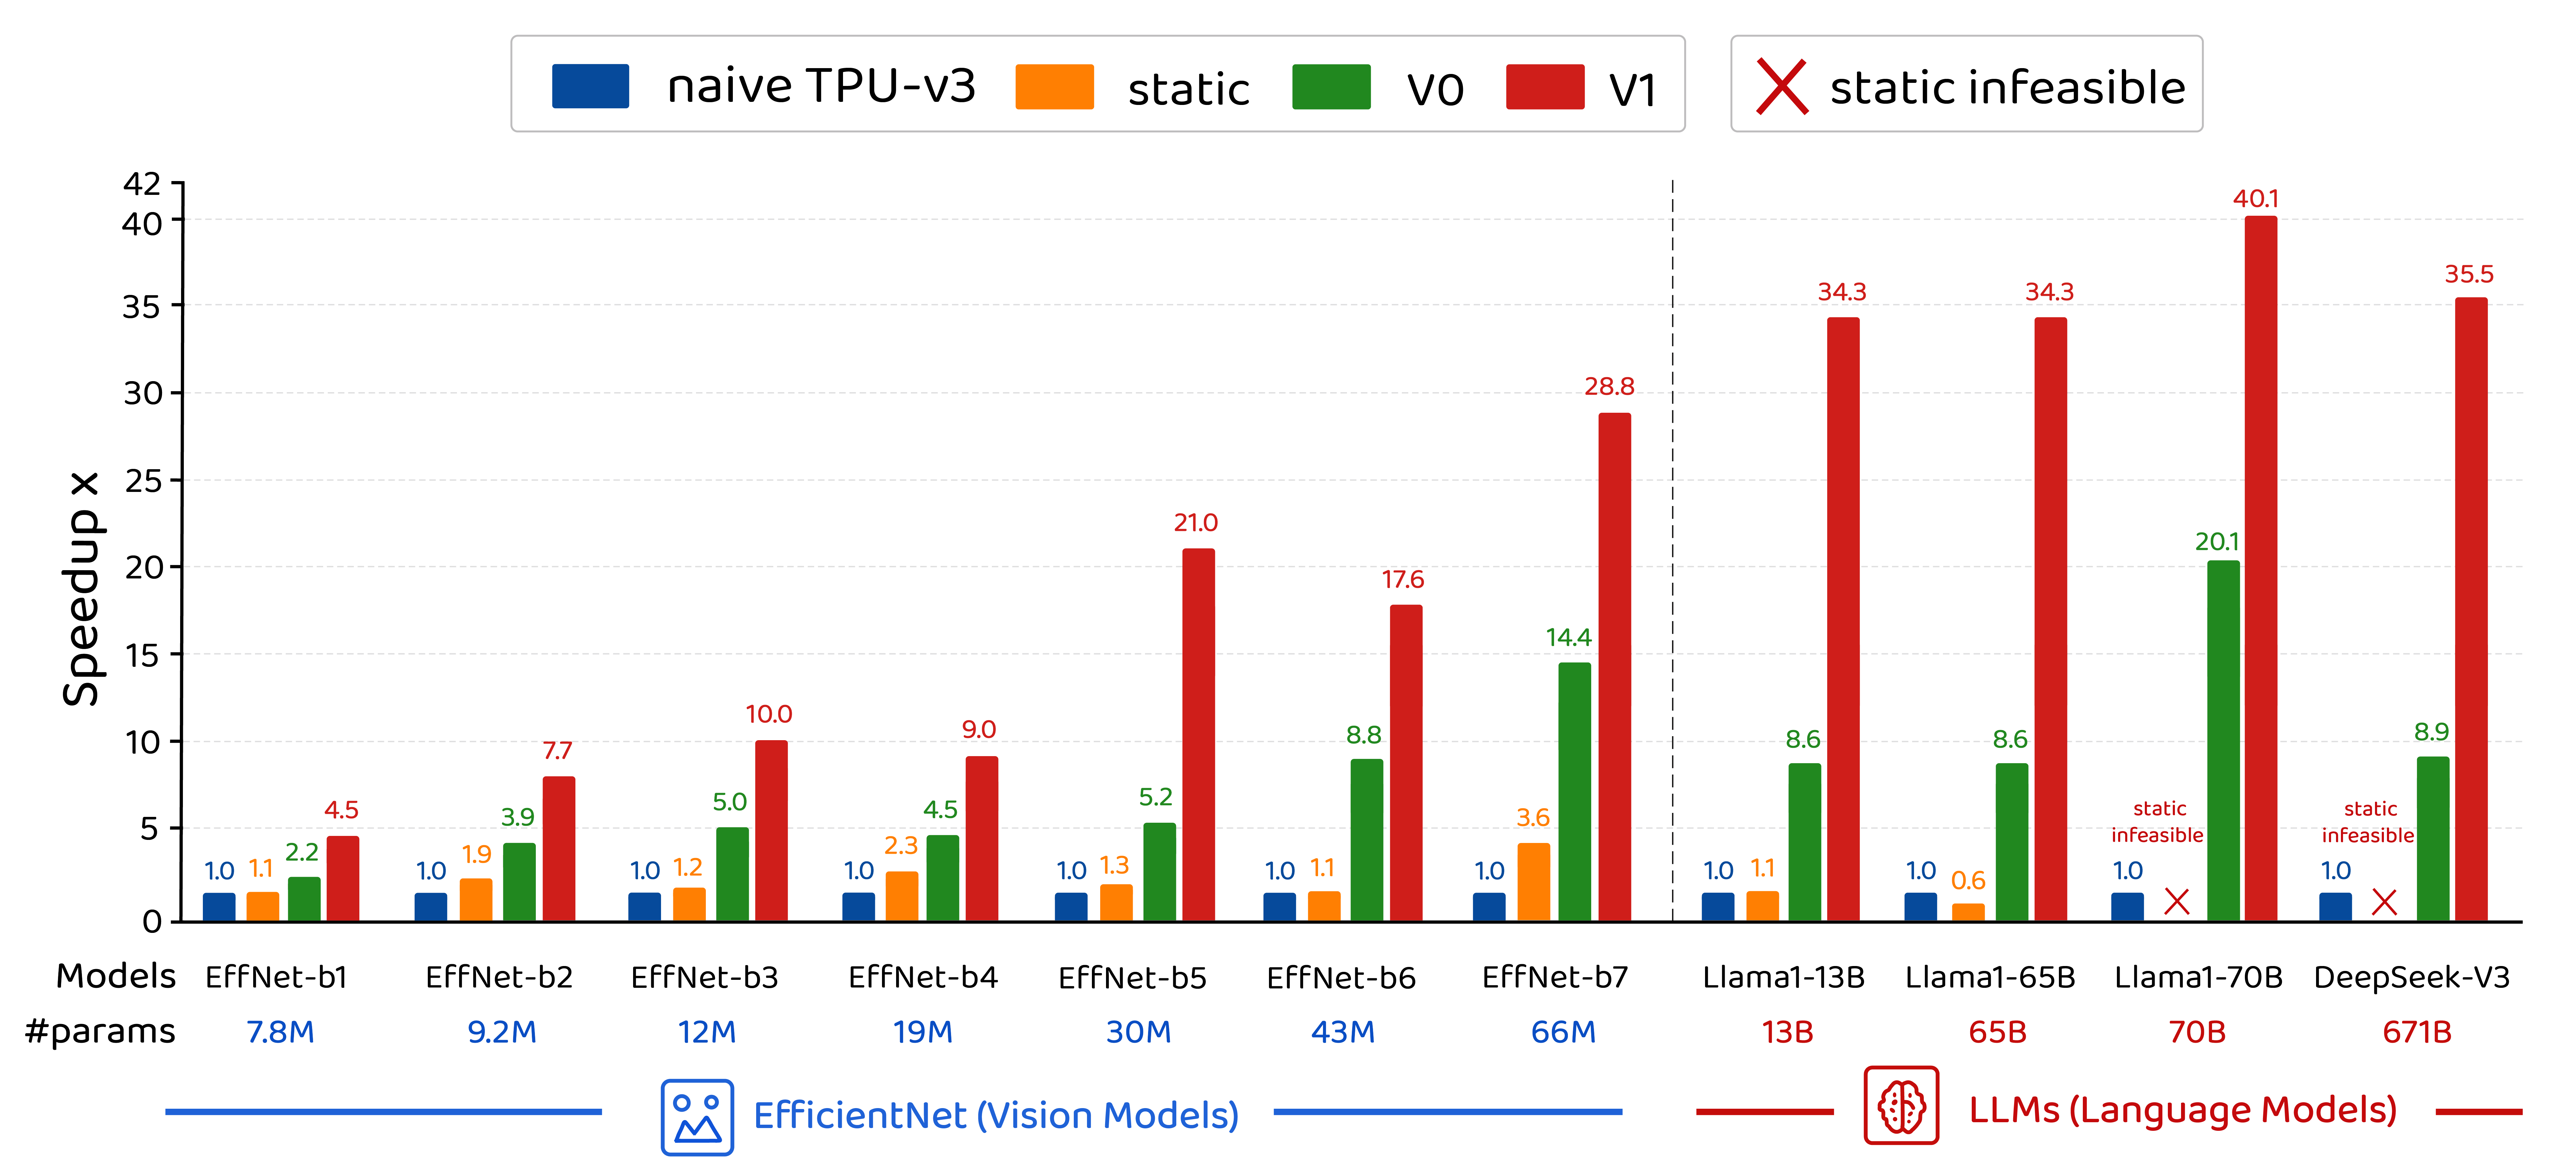
\includegraphics[width=1.0\linewidth]{fig3/speedup_final_v2.png}
% % % \caption{Speedup over modeled TPU-v3 baseline across formulations and workloads: CHEETAH-V1's joint tiling-fusion optimization achieves up to $\sim$35× acceleration, while static fusion is infeasible on large-scale LLMs.}
% % % \label{fig:speedup}
% % % \end{figure}

% % % % In addition to efficiently enabling more globally optimized accelerator designs, we anticipate that future work may build off this foundation to implement custom Flash Attention type speedup mechanisms for individual hardware (such as RTX5090) and workloads (such as LLama70B) tractably within hours, as well as quickly and efficiently design custom accelerators for targeted inference tasks. 
% % % % compromise on any single workload; a growing body of evidence suggests that workload-specialized designs can deliver $2$--$6\times$ improvements in performance per watt.
% % % % The resulting system replaces FAST's sequential Timeloop$\rightarrow$fusion~ILP pipeline with a single LP that jointly optimizes tiling, fusion, and memory scheduling, while preserving Vizier's outer loop over hardware configurations (or replacing it with LLM-guided search).

% % % % Furthermore, FAST's fusion ILP uses static tensor placement: a tensor is either pinned for the entire inference pass or not at all.
% % % % This is overly conservative for models with long dependency chains or skip connections, where different tensors are live at different times during execution.
% % % % A dynamic placement strategy that can evict and re-pin tensors across timesteps could substantially improve global memory utilization. Joint Optimization is the only way to solve the "Memory Wall" for large scale models like DeepSeek-V3.

% % % % FAST operates via a three-stage sequential pipeline (Figure \ref{fig::workflow}): (1)~a black-box optimizer (Google Vizier \citep{google_vizier}) proposes a hardware configuration defined by 16 hyperparameters---PE grid dimensions, systolic array sizes, buffer capacities, DRAM channels, and batch size; (2)~a scheduling engine (Timeloop \citep{timeloop}) finds the best tiling and mapping for each operation independently given the fixed hardware; and (3)~an integer linear program (ILP) decides which tensors to pin in the on-chip Global Memory to reduce DRAM traffic.
% % % % The result of each trial---predicted performance per TDP---is fed back to Vizier, which proposes the next hardware configuration, repeating for thousands of trials until convergence.


% % % % automate the framework with SkyDiscover Loop for profile and context aware co-design. Therefore in less than five hours, we are able to find an more performant design spec than the strongest baseline on designing , in terms of both perf/TDP and speedup. Our experiments also include freezing any hardware at input, and reducing the scheduling, tiling, etc search to just the LP can yield speedups of avg 2.2x than just the base hardware along. We anticipate that future work may build off this foundation to implement custom Flash Attention type speedup mechanisms for individual hardware (such as RTX5090) and workloads (such as LLama70B) tractably within hours. 

% % % % Our propose the formulation for global co-design for a custom accelerator as a large scale linear program which captures strict dependencies and tradeoffs sequential methods may miss. Our LP formulation captures scheduling, tiling, rematerialization, and is able to solve matrices at scales of $6{,}319 \times 4{,}516$,\ nnz$=829{,}852$ \& $3{,}669{,}793 \times 3{,}263{,}443$,\ nnz$=7{,}342{,}293$ \& $2{,}983{,}450 \times 2{,}504{,}019$,\ nnz$=6{,}094{,}156$ quickly, by utilizing a JAX based large scale solver. Our insight is that despite the challenging large scale of the problem, the structure of the matrices, once formed, retain the same structure. Therefore we are able to design one preconditioning scheme to these large scale systems matrices that can be re-used across any NN. This also allows us to capture dependencies prior methods cannot, for example our formulation introduces a dynamic placement strategy that can evict and re-pin tensors across timesteps could substantially improve global memory utilization. Joint Optimization is the only way to solve the "Memory Wall" for large scale models like DeepSeek-V3. 

% % % % For EfficientNet-B7 at $L=400$ operations and $T=400$ timesteps, the V1 LP contains approximately $2$ million variables and $5$ million constraints with $15$--$25$ million nonzeros. To better solve such large-scale LP problems more efficiently, we implement our own variant of a GPU-accelerated solver based on recent primal-dual LP algorithm \citep{applegate2022practicallargescalelinearprogramming}. We extend its original formulation in various ways and benchmark our implementation compared to existing commercial SciPy solvers, which showcase the advantage of our solver. To keep the main context clean and focused, we defer LP solver-related details to Appendix \ref{app:solver}.

% % % % A large number of black box optimization tools to handle this large search space have been recently proposed, such as Google's Vizier, Meta's AX, and Optuna. In addition search strategies are also explored, for example Google's Vizier proposes numerous methods Gaussian Process Upper Confidence Bound, Eagle Strategy as a metaheuristic optimization algorithm designed for global optimization via a two-stage hybrid approach that combines global exploration with intensive local search, and Linear Combination Swarm (LCS). However these methods share certain limitations, since they cannot globally capture the tradeoffs and tensions between sequential decisions and rely on brute force iterations. This requires human engineers to spend months of compute and thousands of repetitive trials to get improvements, without feedback on what might be globally optimal. 

% % % % While this sequential decomposition makes the problem tractable, it introduces a fundamental limitation: \emph{each stage takes the previous stage's output as fixed input, preventing the discovery of solutions that require trading off across stages.} Consider a concrete example: for a depthwise-separable convolution layer in a NN, a search tool such as Timeloop might select a tiling configuration that maximizes compute utilization at $74\%$, producing an activation working set of $6$ MiB. THe stacked The downstream fusion ILP solver tool receives this fixed working set size, cannot fit the tensor into the $128$ MiB Global Memory alongside other pinned tensors. However, an alternative tiling configuration with slightly lower utilization ($70\%$) might produce a working set of only $3$ MiB, enabling the fusion solver to pin an additional weight tensor that eliminates a DRAM bottleneck entirely, thus yielding a net $>20\%$ cycle reduction despite the $4\%$ utilization loss. Therefore these sequential pipelines systematically misses such cross-stage trade-offs.

% % % % The rapid evolution of deep learning workloads has created a compelling opportunity for domain-optimized inference accelerators.
% % % % Production models now serve billions of daily users, and the computational demands of architectures based on depthwise-separable convolutions (EfficientNet), self-attention (BERT, LLaMA), mixture-of-experts (DeepSeek-V3, Mixtral), and state-space models (Mamba) differ dramatically in their compute-to-memory ratios, tensor shapes, and data reuse patterns. However although the NN training strategy has been scaled up and we've done a lot of work on it, we now face the inference bottle neck era since general-purpose hardware, Nvidia's gaming GPUs are not necessarily optimized for deep learning tasks, and leaves a huge amount of compute on the table.


% % % page edit

% % \section{Introduction}
% % \label{sec:introduction}

% % \begin{figure}[ht!]
% %     \centering
% %     \includegraphics[width=1.0\linewidth]{figs/cheetah_v4.png}
% %     % \caption{\textbf{FAST vs.\ FAST-CORGI pipeline comparison.} 
% % \caption{Sequential vs Our Unified Optimization Paradigm.
% % (Left) Baseline methods decouple hardware search, operation-level tiling, and static fusion; precluding cross-stage trade-offs.
% % (Right) CHEETAH presents a unified LLM-driven LP-solver-based framework that jointly optimizes tiling, placement, and rematerialization while learning from a causal ledger.}
% % \label{fig::workflow}
% % \end{figure}
% % % The rapid evolution of deep learning workloads varies from convolutions to self-attention (LLaMA), mixture-of-experts (DeepSeek-V3), and state-space models (Mamba). These diverse architectures serve billions of daily users, and have fundamentally shifted the requirements for hardware acceleration. As foundation models continue to scale in parameters, the primary cost and bottleneck of model deployment has shifted from training to inference. Therefore much recent research has been focused on optimizing for more efficient execution and throughput across diverse, high-dimensional workloads. General-purpose GPUs remain largely designed for graphics-heavy throughput, and leave substantial efficiency and compute on the table at these tasks. Therefore we are motivated to design targeted accelerators that are optimized for handling the varying tensor shapes and data-reuse patterns of modern deep learning architectures.
% % % Much research has been done in accelerating inference through custom accelerator design, more efficient neural network (NN) batching algorithms, and domain specific packages and languages that aim to speed up general NN inference. For example, the widely adopted Flash Attention uses tiling to provide significant speedups by optimizing memory movement between SRAM and DRAM. Co-design takes this a step further by aiming to optimize hardware, software and scheduling to unlock performance neither could reach independently. The traditional framework of doing this is a sequential pipeline of heuristics tools, requiring human engineers to iterate through a large search space for months from testing for the size of DRAM, to determining higher level scheduling problems. Optimizing each piece of this complex pipeline is extremely challenging, since hardware datapaths, software schedules, and compiler transforms across a combinatorial space exceeding $\mathcal O(10^{2300})$.
% % The AI inference demand is expected to grow by $10,000\times$ over the next 5 years \citep{cra2026aifuture}. General-purpose accelerators leave significant efficiency gains unrealized, which motivates the design of targeted custom accelerators. Co-design, which jointly optimizes hardware-software (HW/SW), and scheduling for target workloads, offers a path to unlock performance efficiency for the upcoming inference era. However, the prevailing approach relies on sequential pipelines of heuristic tools, a slow, human-driven process navigating a combinatorial search space exceeding $O(10^{2300})$ \citep{zhang_fast}. State-of-the-art frameworks like FAST \citep{zhang_fast} improve on this through an automated flow (a hardware proposer feeds an operation-level tiling agent, which feeds a downstream fusion solver), but remain fundamentally decoupled: a tiling that slightly reduces compute efficiency may shrink the working set enough to eliminate a DRAM bottleneck, yet sequential pipelines cannot discover such cross-stage trade-offs.

% % % The co-design problem is increasingly important as inference efficiency is the dominant AI workload and is rapidly growing. Therefore industry leaders such as NVIDIA and Google have designed chips for improved hardware-native agentic AI and , and state-of-the-art frameworks such as FAST, address this through a sequential decomposition of heuristics (a hardware proposer feeds an operation-level tiling agent, which feeds a downstream fusion solver). While FAST-generated accelerators can provide increased speedups over baseline TPU-v3, this decoupled approach is limited since it cannot capture cross-stage trade-offs. A tiling configuration that is \textit{locally} optimal for one layer may create an activation footprint that later prevents \textit{global} fusion, while a slightly slower tiling might shrink the working set enough to eliminate a DRAM bottleneck entirely. Sequential pipelines are systematically unable to express these interactions, leading to locally good but globally sub-optimal designs. 
% % Unifying the design space into a single convex relaxation yields previously infeasible global optima. Specifically, we introduce CHEETAH: a custom inference accelerator design framework that unlocks globally optimized designs with a dual-loop. Our inner-loop is a novel large-scale Linear Program (LP) to precisely mathematically model strict design decisions and constraints that must not be violated. The LP captures trade-offs for targeted workloads through time-indexed placement and rematerialization, thus allowing tensors to be dynamically pinned, evicted, recomputed across inference timesteps. We further extend our reformulation to internalize tiling selection into the LP, by introducing Pareto-pruned tiling variables and the McCormick linearization (a convex relaxation used for optimization of bilinear problems \citep{mccormick1976computability}). By exploiting the structural invariance of our matrices across hardware trials, we also adapt a GPU-accelerated primal-dual solver in JAX \citep{jax2018github} that can resolve millions of variables to rapidly reduce trial time from days to hours. This allows the LP solver to jointly reason about hardware configuration, activation placement, and weight pinning in a single pass, while providing feedback signal via Lagrangian duals.

% % Our outer-loop framework stacks a black-box optimizer (Google Vizier \citep{google_vizier}) to propose candidate hardware configurations defined by a set of hyperparameters (e.g., processing element grid dimensions, systolic array sizes, DRAM size, etc), while a LLM is used for efficient search-space steering. The LLM acts as a causal architect, interpreting a compact trial ledger of roofline checks and LP feedback diagnostics to propose constrained architectural search input for Vizier. This prevents the search-space gaming typical of black-box optimizers in wide design regions, and reduces the need for thousands of sequential trials via Bayesian search strategies in Vizier to learn good vs bad neighborhoods in search topology. Our results demonstrate that the LLM Architect framework further reduces invalid hardware trials from 24.5\% under vanilla Vizier to 5.9\%, while reaching the Pareto frontier 4.5x faster than the next strongest baseline. We validate all results with Model Flop Utilization (MFU) and roofline lower-bound audits, ensuring predicted latencies are physically grounded in compute and memory throughput limits. 
% % % \todo{Add best of both worlds, strengths from principled LP side, from LLM aggregate info side}
% % % \todo{Aggregates past experience to gain insight into steering hardware-software co-design. We offload the strict solves, with constraints that must the strictly respected, to the LP solve part. This combines the best of both worlds.} 
% % \paragraph{Contributions.} We reformulated the fundamental HW/SW co-design problem into a unified  framework in CHEETAH, combining principled mathematical rigor of the LP formulation to solve strict design decisions optimally, with the powerful aggregation and causal learning of an LLM Architect outer loop for meta-optimization. Our open-source repository for full reproducibility is at \href{https://anonymous.4open.science/r/CHEETAH-B268/readme}{https://anonymous.4open.science/r/CHEETAH-B268/}.

% % \begin{enumerate}
% %     \item \textbf{CHEETAH-V0 - Dynamic Placement with Rematerialization:}
% %     We introduce time-indexed LP variables $p_{i,t}^k$ and rematerialization variables $r_{i,t}$ to enable cheap recompute operations instead of paying DRAM reload costs, supporting skip connections and multi-fanout nodes.

% %     \item \textbf{CHEETAH-V1 - Joint Tiling-Fusion:}
% %     We unify tiling and fusion into a single LP problem by introducing tiling selection variables $y_{i,c}$, and employ McCormick envelopes to exactly linearize the bilinear interaction between tiling and tensor pinning. This technique yields a tight, parameter-free LP relaxation, and the coupling internalizes the tiling-placement trade-off to discover optimal design points that sequential pipelines systematically miss.
% %     % This enables the LP to discover trade-offs where accepting a suboptimal tiling configuration enables superior fusion, or vice versa---precisely the cross-stage interactions that the sequential pipeline cannot capture.
% %     \item \textbf{LLM-guided Causal Architect:} The LLM outer loop steers hardware search by interpreting Lagrangian sensitivity signals and a Causal Ledger of past trials to perform targeted subspace interventions, transforming black-box search into a structured, diagnostic-driven process. The Architect guides Vizier through widened search spaces, reducing invalid trials by ${\sim}4\times$ while preserving the global optimal score, and enables profile-specific designs (speech models may emphasize latency, while data synthesis models may prioritize bandwidth). 
% %     \item \textbf{Speedup:} Our method demonstrates an average speedup of $\sim22.07\times$ over the baseline across a wide range of $11$ vision and language models. 

% %     % profiles into consideration to push the black-box optimizer responsible for hardware suggestions to output with structured reasoning about architectural trade-offs. 

% % \end{enumerate}

% % \begin{figure}[ht!]
% %     \centering
% % 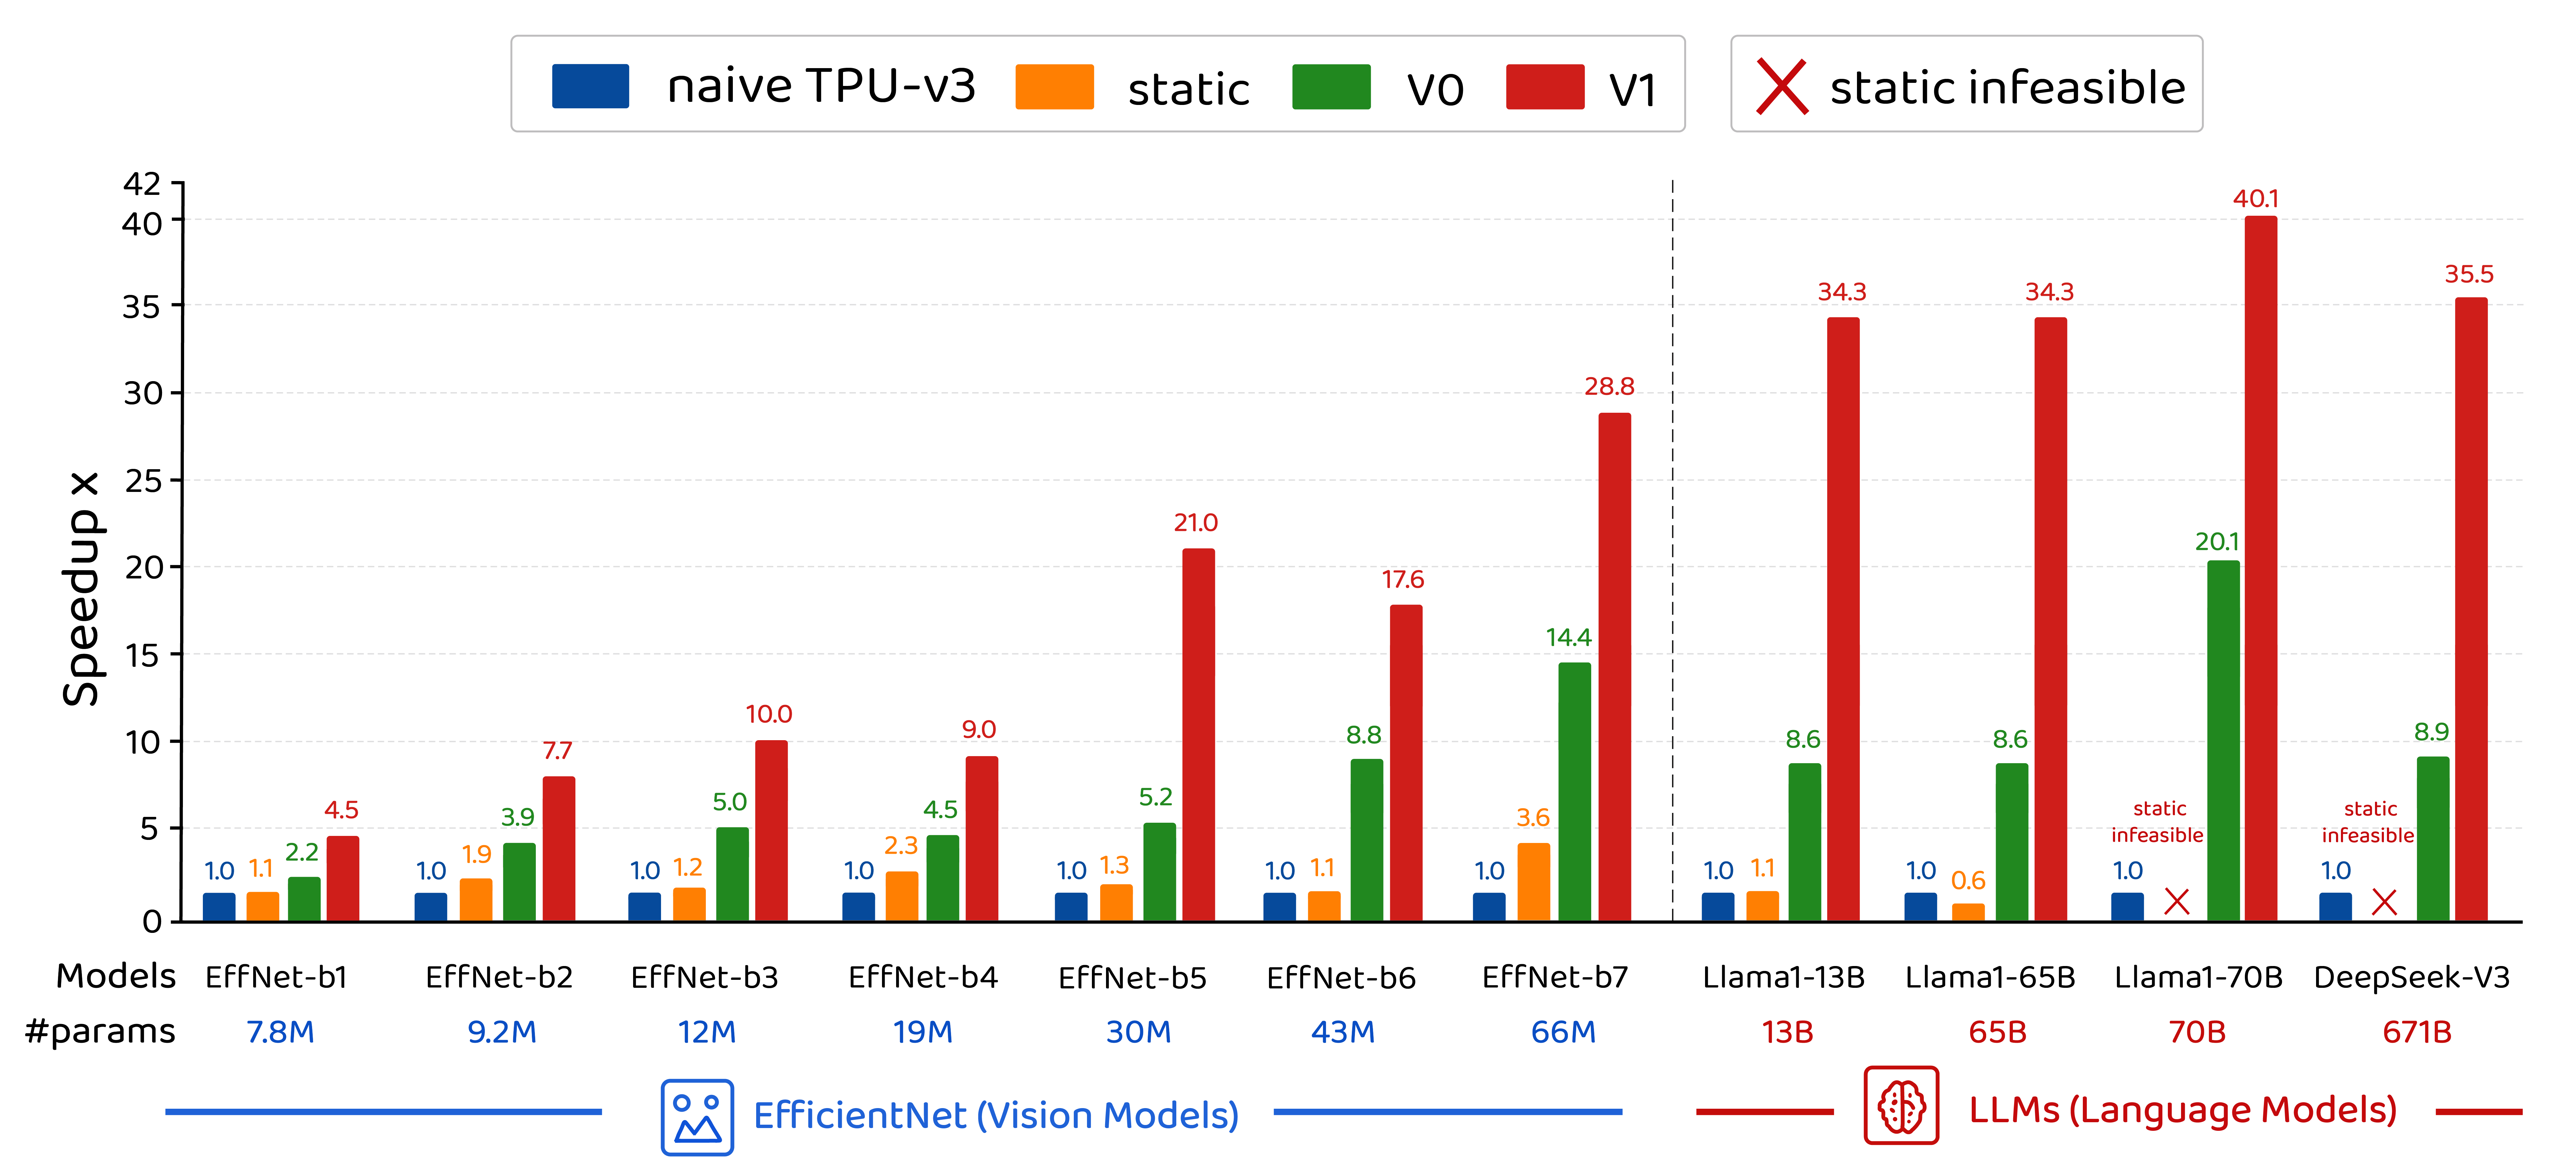
\includegraphics[width=1.0\linewidth]{fig3/speedup_final_v2.png}
% % \caption{Speedup over modeled TPU-v3 baseline across formulations and workloads: CHEETAH-V1's joint tiling-fusion optimization achieves up to $\sim$40.1$\times$ acceleration, while static fusion is infeasible on large-scale LLMs. Progressive gains are visible across formulations: V0's dynamic placement improves over static by $2$--$20\times$, while V1's joint tiling-fusion adds another $2$--$4\times$ on top. See Section~\ref{sec:experiments} for full analysis and wall-clock time breakdowns.}
% % \label{fig:speedup}
% % \end{figure}

% % % In addition to efficiently enabling more globally optimized accelerator designs, we anticipate that future work may build off this foundation to implement custom Flash Attention type speedup mechanisms for individual hardware (such as RTX5090) and workloads (such as LLama70B) tractably within hours, as well as quickly and efficiently design custom accelerators for targeted inference tasks. 
% % % compromise on any single workload; a growing body of evidence suggests that workload-specialized designs can deliver $2$--$6\times$ improvements in performance per watt.
% % % The resulting system replaces FAST's sequential Timeloop$\rightarrow$fusion~ILP pipeline with a single LP that jointly optimizes tiling, fusion, and memory scheduling, while preserving Vizier's outer loop over hardware configurations (or replacing it with LLM-guided search).

% % % Furthermore, FAST's fusion ILP uses static tensor placement: a tensor is either pinned for the entire inference pass or not at all.
% % % This is overly conservative for models with long dependency chains or skip connections, where different tensors are live at different times during execution.
% % % A dynamic placement strategy that can evict and re-pin tensors across timesteps could substantially improve global memory utilization. Joint Optimization is the only way to solve the "Memory Wall" for large scale models like DeepSeek-V3.

% % % FAST operates via a three-stage sequential pipeline (Figure \ref{fig::workflow}): (1)~a black-box optimizer (Google Vizier \citep{google_vizier}) proposes a hardware configuration defined by 16 hyperparameters---PE grid dimensions, systolic array sizes, buffer capacities, DRAM channels, and batch size; (2)~a scheduling engine (Timeloop \citep{timeloop}) finds the best tiling and mapping for each operation independently given the fixed hardware; and (3)~an integer linear program (ILP) decides which tensors to pin in the on-chip Global Memory to reduce DRAM traffic.
% % % The result of each trial---predicted performance per TDP---is fed back to Vizier, which proposes the next hardware configuration, repeating for thousands of trials until convergence.


% % % automate the framework with SkyDiscover Loop for profile and context aware co-design. Therefore in less than five hours, we are able to find an more performant design spec than the strongest baseline on designing , in terms of both perf/TDP and speedup. Our experiments also include freezing any hardware at input, and reducing the scheduling, tiling, etc search to just the LP can yield speedups of avg 2.2x than just the base hardware along. We anticipate that future work may build off this foundation to implement custom Flash Attention type speedup mechanisms for individual hardware (such as RTX5090) and workloads (such as LLama70B) tractably within hours. 

% % % Our propose the formulation for global co-design for a custom accelerator as a large scale linear program which captures strict dependencies and tradeoffs sequential methods may miss. Our LP formulation captures scheduling, tiling, rematerialization, and is able to solve matrices at scales of $6{,}319 \times 4{,}516$,\ nnz$=829{,}852$ \& $3{,}669{,}793 \times 3{,}263{,}443$,\ nnz$=7{,}342{,}293$ \& $2{,}983{,}450 \times 2{,}504{,}019$,\ nnz$=6{,}094{,}156$ quickly, by utilizing a JAX based large scale solver. Our insight is that despite the challenging large scale of the problem, the structure of the matrices, once formed, retain the same structure. Therefore we are able to design one preconditioning scheme to these large scale systems matrices that can be re-used across any NN. This also allows us to capture dependencies prior methods cannot, for example our formulation introduces a dynamic placement strategy that can evict and re-pin tensors across timesteps could substantially improve global memory utilization. Joint Optimization is the only way to solve the "Memory Wall" for large scale models like DeepSeek-V3. 

% % % For EfficientNet-B7 at $L=400$ operations and $T=400$ timesteps, the V1 LP contains approximately $2$ million variables and $5$ million constraints with $15$--$25$ million nonzeros. To better solve such large-scale LP problems more efficiently, we implement our own variant of a GPU-accelerated solver based on recent primal-dual LP algorithm \citep{applegate2022practicallargescalelinearprogramming}. We extend its original formulation in various ways and benchmark our implementation compared to existing commercial SciPy solvers, which showcase the advantage of our solver. To keep the main context clean and focused, we defer LP solver-related details to Appendix \ref{app:solver}.

% % % A large number of black box optimization tools to handle this large search space have been recently proposed, such as Google's Vizier, Meta's AX, and Optuna. In addition search strategies are also explored, for example Google's Vizier proposes numerous methods Gaussian Process Upper Confidence Bound, Eagle Strategy as a metaheuristic optimization algorithm designed for global optimization via a two-stage hybrid approach that combines global exploration with intensive local search, and Linear Combination Swarm (LCS). However these methods share certain limitations, since they cannot globally capture the tradeoffs and tensions between sequential decisions and rely on brute force iterations. This requires human engineers to spend months of compute and thousands of repetitive trials to get improvements, without feedback on what might be globally optimal. 

% % % While this sequential decomposition makes the problem tractable, it introduces a fundamental limitation: \emph{each stage takes the previous stage's output as fixed input, preventing the discovery of solutions that require trading off across stages.} Consider a concrete example: for a depthwise-separable convolution layer in a NN, a search tool such as Timeloop might select a tiling configuration that maximizes compute utilization at $74\%$, producing an activation working set of $6$ MiB. THe stacked The downstream fusion ILP solver tool receives this fixed working set size, cannot fit the tensor into the $128$ MiB Global Memory alongside other pinned tensors. However, an alternative tiling configuration with slightly lower utilization ($70\%$) might produce a working set of only $3$ MiB, enabling the fusion solver to pin an additional weight tensor that eliminates a DRAM bottleneck entirely, thus yielding a net $>20\%$ cycle reduction despite the $4\%$ utilization loss. Therefore these sequential pipelines systematically misses such cross-stage trade-offs.

% % % The rapid evolution of deep learning workloads has created a compelling opportunity for domain-optimized inference accelerators.
% % % Production models now serve billions of daily users, and the computational demands of architectures based on depthwise-separable convolutions (EfficientNet), self-attention (BERT, LLaMA), mixture-of-experts (DeepSeek-V3, Mixtral), and state-space models (Mamba) differ dramatically in their compute-to-memory ratios, tensor shapes, and data reuse patterns. However although the NN training strategy has been scaled up and we've done a lot of work on it, we now face the inference bottle neck era since general-purpose hardware, Nvidia's gaming GPUs are not necessarily optimized for deep learning tasks, and leaves a huge amount of compute on the table.

% % refer tofigure 2 edit

% % \section{Introduction}
% % \label{sec:introduction}

% % \begin{figure}[ht!]
% %     \centering
% %     \includegraphics[width=1.0\linewidth]{figs/cheetah_v4.png}
% % \caption{Sequential vs Unified Optimization Paradigm Comparison.
% % (Left) Baseline methods decouple hardware search, operation-level tiling, and static fusion; precluding cross-stage trade-offs.
% % (Right) CHEETAH presents a unified LLM-driven LP-solver-based framework that jointly optimizes tiling, placement, and rematerialization while learning from a causal ledger.}
% % \label{fig::workflow}
% % \end{figure}
% % % The rapid evolution of deep learning workloads varies from convolutions to self-attention (LLaMA), mixture-of-experts (DeepSeek-V3), and state-space models (Mamba). These diverse architectures serve billions of daily users, and have fundamentally shifted the requirements for hardware acceleration. As foundation models continue to scale in parameters, the primary cost and bottleneck of model deployment has shifted from training to inference. Therefore much recent research has been focused on optimizing for more efficient execution and throughput across diverse, high-dimensional workloads. General-purpose GPUs remain largely designed for graphics-heavy throughput, and leave substantial efficiency and compute on the table at these tasks. Therefore we are motivated to design targeted accelerators that are optimized for handling the varying tensor shapes and data-reuse patterns of modern deep learning architectures.
% % % Much research has been done in accelerating inference through custom accelerator design, more efficient neural network (NN) batching algorithms, and domain specific packages and languages that aim to speed up general NN inference. For example, the widely adopted Flash Attention uses tiling to provide significant speedups by optimizing memory movement between SRAM and DRAM. Co-design takes this a step further by aiming to optimize hardware, software and scheduling to unlock performance neither could reach independently. The traditional framework of doing this is a sequential pipeline of heuristics tools, requiring human engineers to iterate through a large search space for months from testing for the size of DRAM, to determining higher level scheduling problems. Optimizing each piece of this complex pipeline is extremely challenging, since hardware datapaths, software schedules, and compiler transforms across a combinatorial space exceeding $\mathcal O(10^{2300})$.
% % The AI inference demand is expected to grow by $10,000\times$ over the next 5 years \citep{cra2026aifuture}. General-purpose accelerators leave significant efficiency gains unrealized, which motivates the design of targeted custom accelerators. Co-design, which jointly optimizes hardware, software, and scheduling for target workloads, offers a path to unlock performance efficiency for the upcoming inference era. However, the prevailing approach relies on sequential pipelines of heuristic tools, a slow, human-driven process navigating a combinatorial search space exceeding $O(10^{2300})$ \citep{zhang_fast}. State-of-the-art frameworks like FAST \citep{zhang_fast} improve on through an automated flow (a hardware proposer feeds an operation-level tiling agent, which feeds a downstream fusion solver), but remain fundamentally decoupled.  For example, a tiling configuration that is \textit{locally} optimal for one layer may create an activation footprint that later prevents \textit{global} fusion, while a slightly slower tiling might shrink the working set enough to eliminate a DRAM bottleneck entirely. Sequential pipelines are systematically unable to express these interactions, leading to locally good but globally sub-optimal designs.

% % % The co-design problem is increasingly important as inference efficiency is the dominant AI workload and is rapidly growing. Therefore industry leaders such as NVIDIA and Google have designed chips for improved hardware-native agentic AI and , and state-of-the-art frameworks such as FAST, address this through a sequential decomposition of heuristics (a hardware proposer feeds an operation-level tiling agent, which feeds a downstream fusion solver). While FAST-generated accelerators can provide increased speedups over baseline TPU-v3, this decoupled approach is limited since it cannot capture cross-stage trade-offs. A tiling configuration that is \textit{locally} optimal for one layer may create an activation footprint that later prevents \textit{global} fusion, while a slightly slower tiling might shrink the working set enough to eliminate a DRAM bottleneck entirely. Sequential pipelines are systematically unable to express these interactions, leading to locally good but globally sub-optimal designs. 
% % We prove that by unifying the design space into a single convex relaxation, we find global optima that were previously  infeasible. Specifically, we introduce CHEETAH: a custom inference accelerator design framework that unlocks globally optimized designs with a dual-loop engine (See Figure \ref{fig::workflow}). Our inner-loop is a novel large-scale Linear Program (LP) to precisely mathematically model strict design decisions and constraints that must not be violated. The LP captures trade-offs for targeted workloads through time-indexed placement and rematerialization, thus allowing tensors to be dynamically pinned, evicted, recomputed across inference timesteps. We further extend our reformulation to internalize tiling selection into the LP, by introducing Pareto-pruned tiling variables and the McCormick linearization (a convex relaxation used for optimization of bilinear problems \citep{mccormick1976computability}). By exploiting the structural invariance of our matrices across hardware trials, we also adapt a GPU-accelerated primal-dual solver in JAX that can resolve millions of variables to rapidly reduce trial time from days to hours. This allows the LP solver to jointly reason about hardware configuration, activation placement, and weight pinning in a single pass, while providing feedback signal via Lagrangian duals.

% % Our outer-loop framework stacks a black-box optimizer (Google Vizier \citep{google_vizier}) to propose candidate hardware configurations defined by a set of hyperparameters (e.g., processing element grid dimensions, systolic array sizes, DRAM size, etc), while a LLM is used for efficient search-space steering. The LLM acts as a causal architect, interpreting a compact trial ledger of roofline checks and LP feedback diagnostics to propose constrained architectural search input for Vizier. This prevents the search-space gaming typical of black-box optimizers in wide design regions, and reduces the need for thousands of sequential trails via Bayesian search strategies in Vizier to learn good vs bad neighborhoods in search topology. Our results demonstrate that the LLM-Architect framework further reduces invalid hardware trials from 24.5\% under vanilla Vizier to 5.9\%, while reaching the Pareto frontier 4.5x faster than the next strongest baseline. We validate all results with Model Flop Utilization (MFU)  and roofline lower-bound audits, ensuring predicted latencies are physically grounded in compute and memory throughput limits. 
% % % \todo{Add best of both worlds, strengths from principled LP side, from LLM aggregate info side}
% % % \todo{Aggregates past experience to gain insight into steering hardware-software co-design. We offload the strict solves, with constraints that must the strictly respected, to the LP solve part. This combines the best of both worlds.} 
% % \paragraph{Contributions.} We reformulated the fundamental HW/SW co-design problem into a unified  framework in CHEETAH, combining principled mathematical rigor of the LP formulation to solve strict design decisions optimally, with the powerful aggregation and causal learning of an LLM Architect outer loop for meta-optimization. Our open-source repository for full reproducibility is at \href{https://anonymous.4open.science/r/CHEETAH-B268/readme}{https://anonymous.4open.science/r/CHEETAH-B268/}.

% % \begin{enumerate}
% %     \item \textbf{CHEETAH-V0 - Dynamic Placement with Rematerialization:}
% %     We introduce the time-indexed and rematerialization variables to enable cheap recompute operations (\eg, depthwise convolutions that account for only $5\%$ of FLOPs but produce large activations) instead of paying DRAM reload costs. This addresses the restrictions of existing baseline methods where activations can only be pinned between consecutively-executed operations, and supports skip connections and multi-fanout nodes.

% %     \item \textbf{CHEETAH-V1 - Joint Tiling-Fusion:}
% %     We unify tiling and fusion into a single LP problem by introducing tiling selection variables $y_{i,c}$, and employ McCormick envelopes to exactly linearize the bilinear interaction between tiling and tensor pinning. This technique yields a tight, parameter-free LP relaxation, and the coupling internalizes the tiling-placement trade-off to discover optimal design points that sequential pipelines systematically miss.
% %     % This enables the LP to discover trade-offs where accepting a suboptimal tiling configuration enables superior fusion, or vice versa---precisely the cross-stage interactions that the sequential pipeline cannot capture.
% %     \item \textbf{LLM-guided Causal Architect:} The LLM outer loop steers hardware search and bridges high-level architectural reasoning with low-level solver duals. It interprets Lagrangian sensitivity signals to perform targeted subspace interventions, transforming black-box search into a structured, diagnostic-driven process. We use a context-aware LLM Architect to propose good search areas as input to Vizier (a black-box Bayesian optimizer). Feedback signals are aggregated across historical trials through both the Causal Ledger and the LP solver. The Architect then guides Vizier through widened search spaces, reducing invalid trials by ${\sim}4\times$ while preserving the global optimal score, while enabling profile-specific designs (speech models may emphasize latency, while data synthesis models may prioritize bandwidth). 
% %     \item \textbf{Speedup:} We show that across a large suite of vision and language modeling workloads, CHEETAH results in an average of 20.9X faster designs than prior work. 

% %     % profiles into consideration to push the black-box optimizer responsible for hardware suggestions to output with structured reasoning about architectural trade-offs. 

% % \end{enumerate}

% % We anticipate that future work may build from this framework in two ways: as an end-to-end co-design system for efficient accelerators, and as an automated optimization engine for existing hardware. By fixing the architecture, the inner loop derives optimal tiling and scheduling strategies that can act as custom speedups for targeted inference tasks.

% % % \begin{figure}[ht!] 
% % %     \centering
% % % 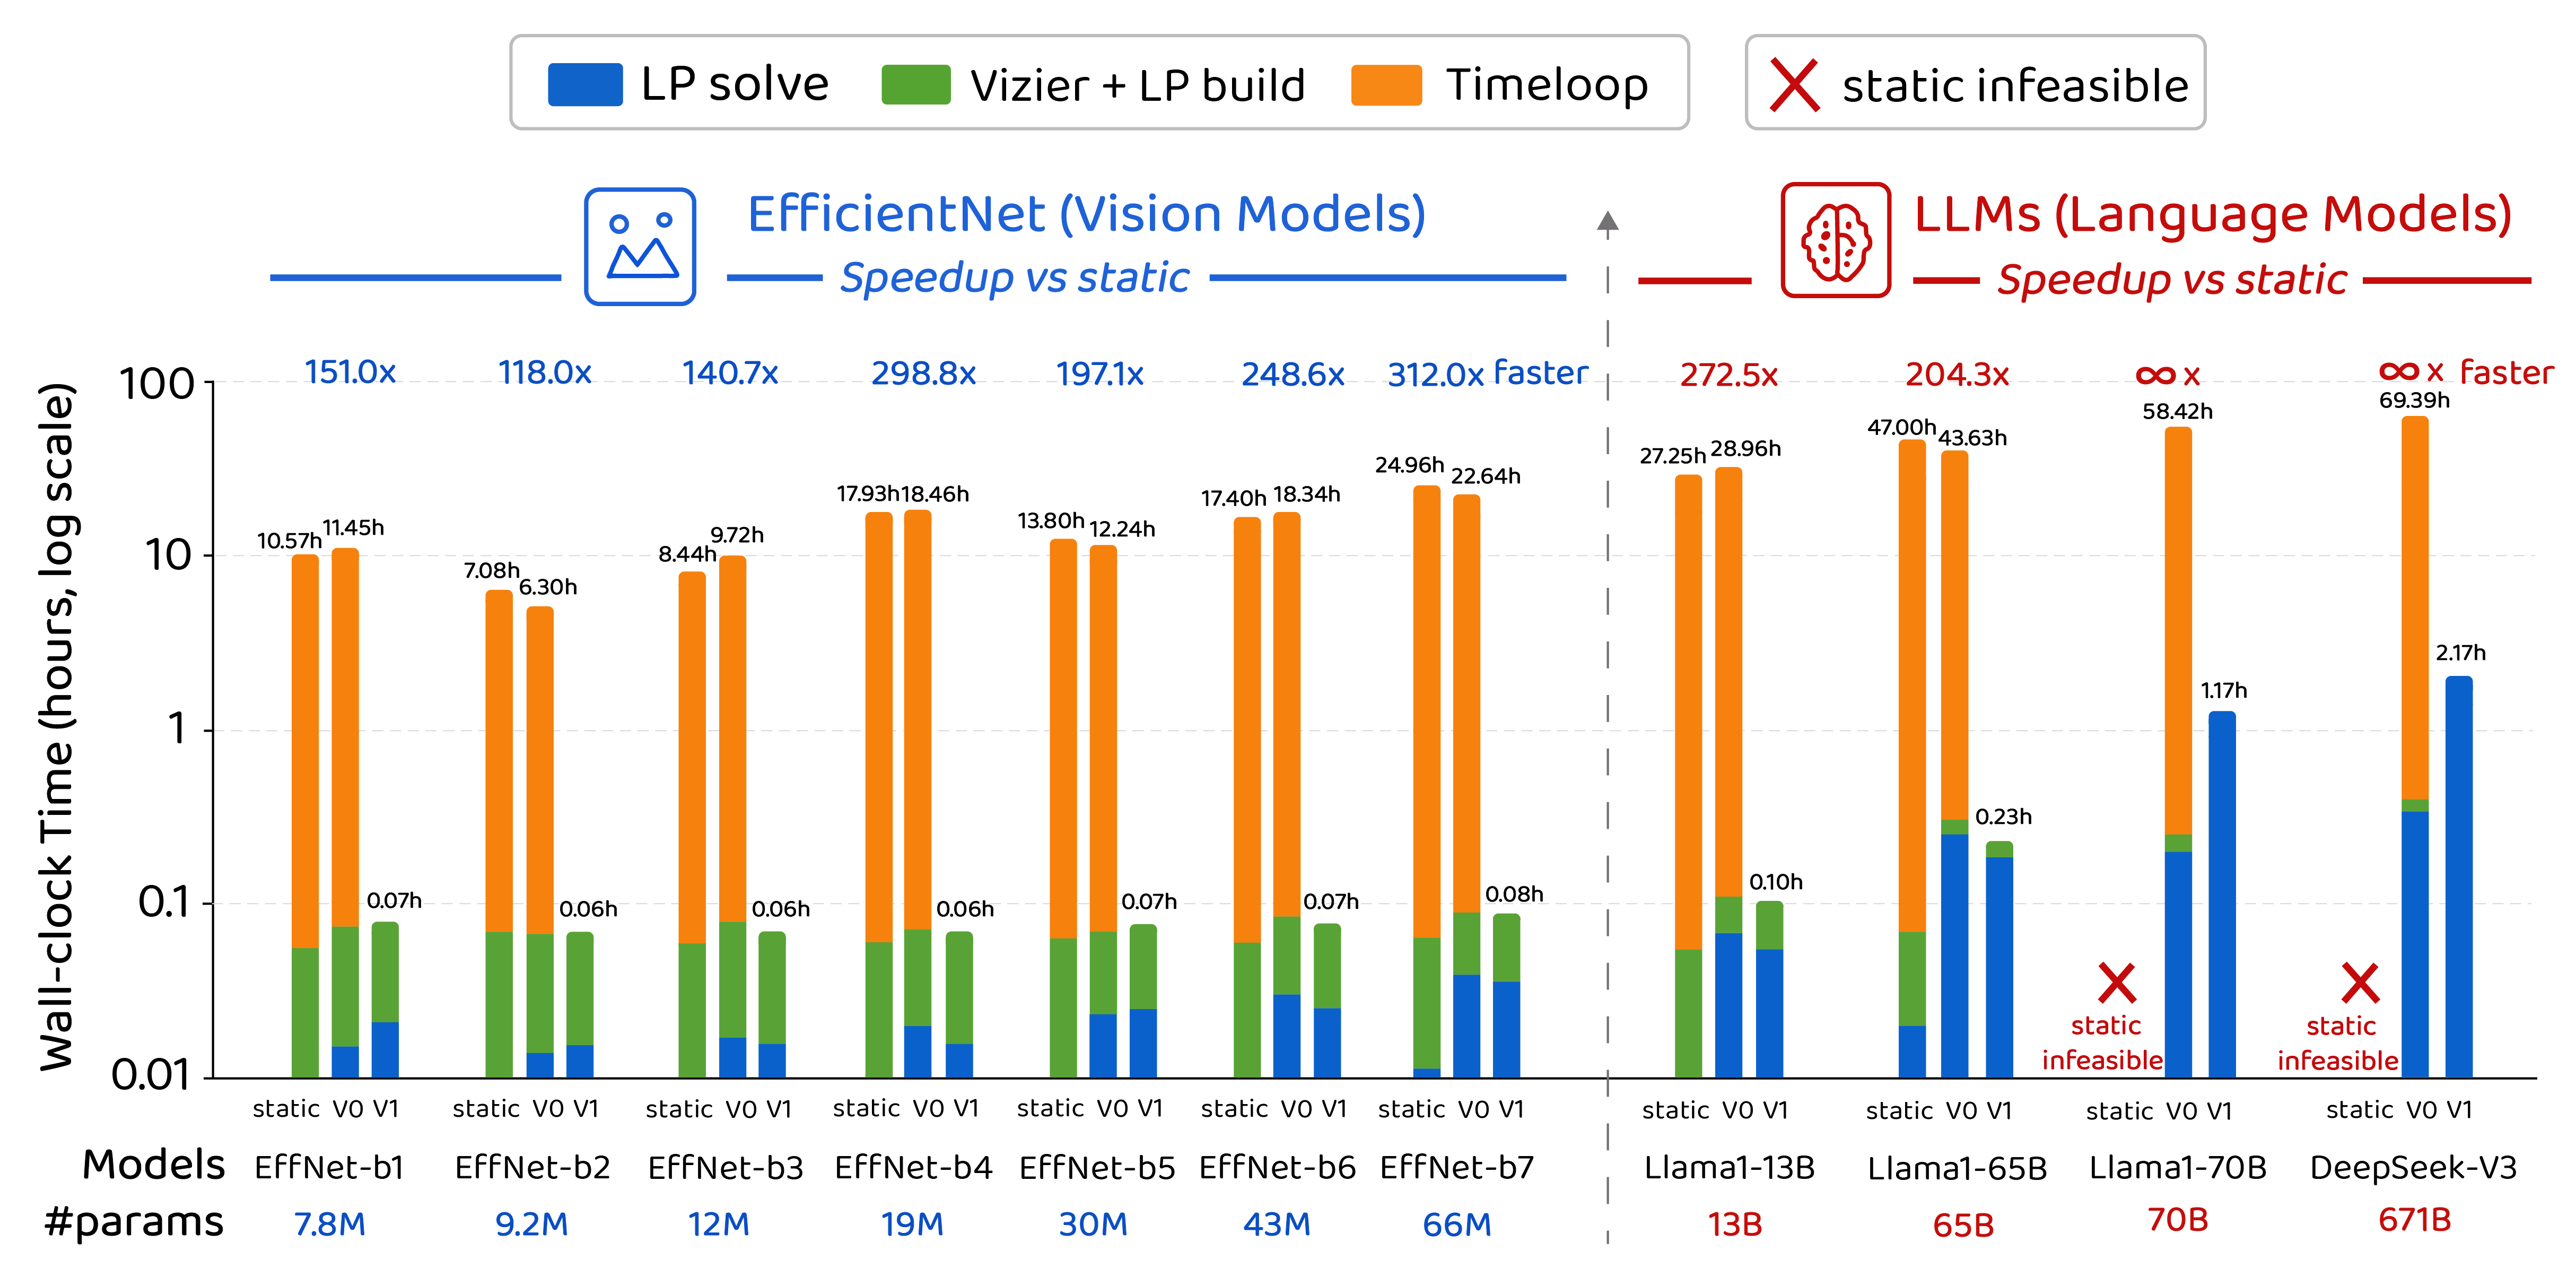
\includegraphics[width=1.0\linewidth]{fig3/wallclock_new_v5.png}
% % % \caption{Wall-clock time decomposition and performance acceleration across formulations: CHEETAH-V1's internalized tiling eliminates the Timeloop bottleneck, achieving up to 100–300× faster search than classical static method.}
% % % \label{fig:wallclock}
% % % \end{figure}

% % \begin{figure}[ht!]
% %     \centering
% % 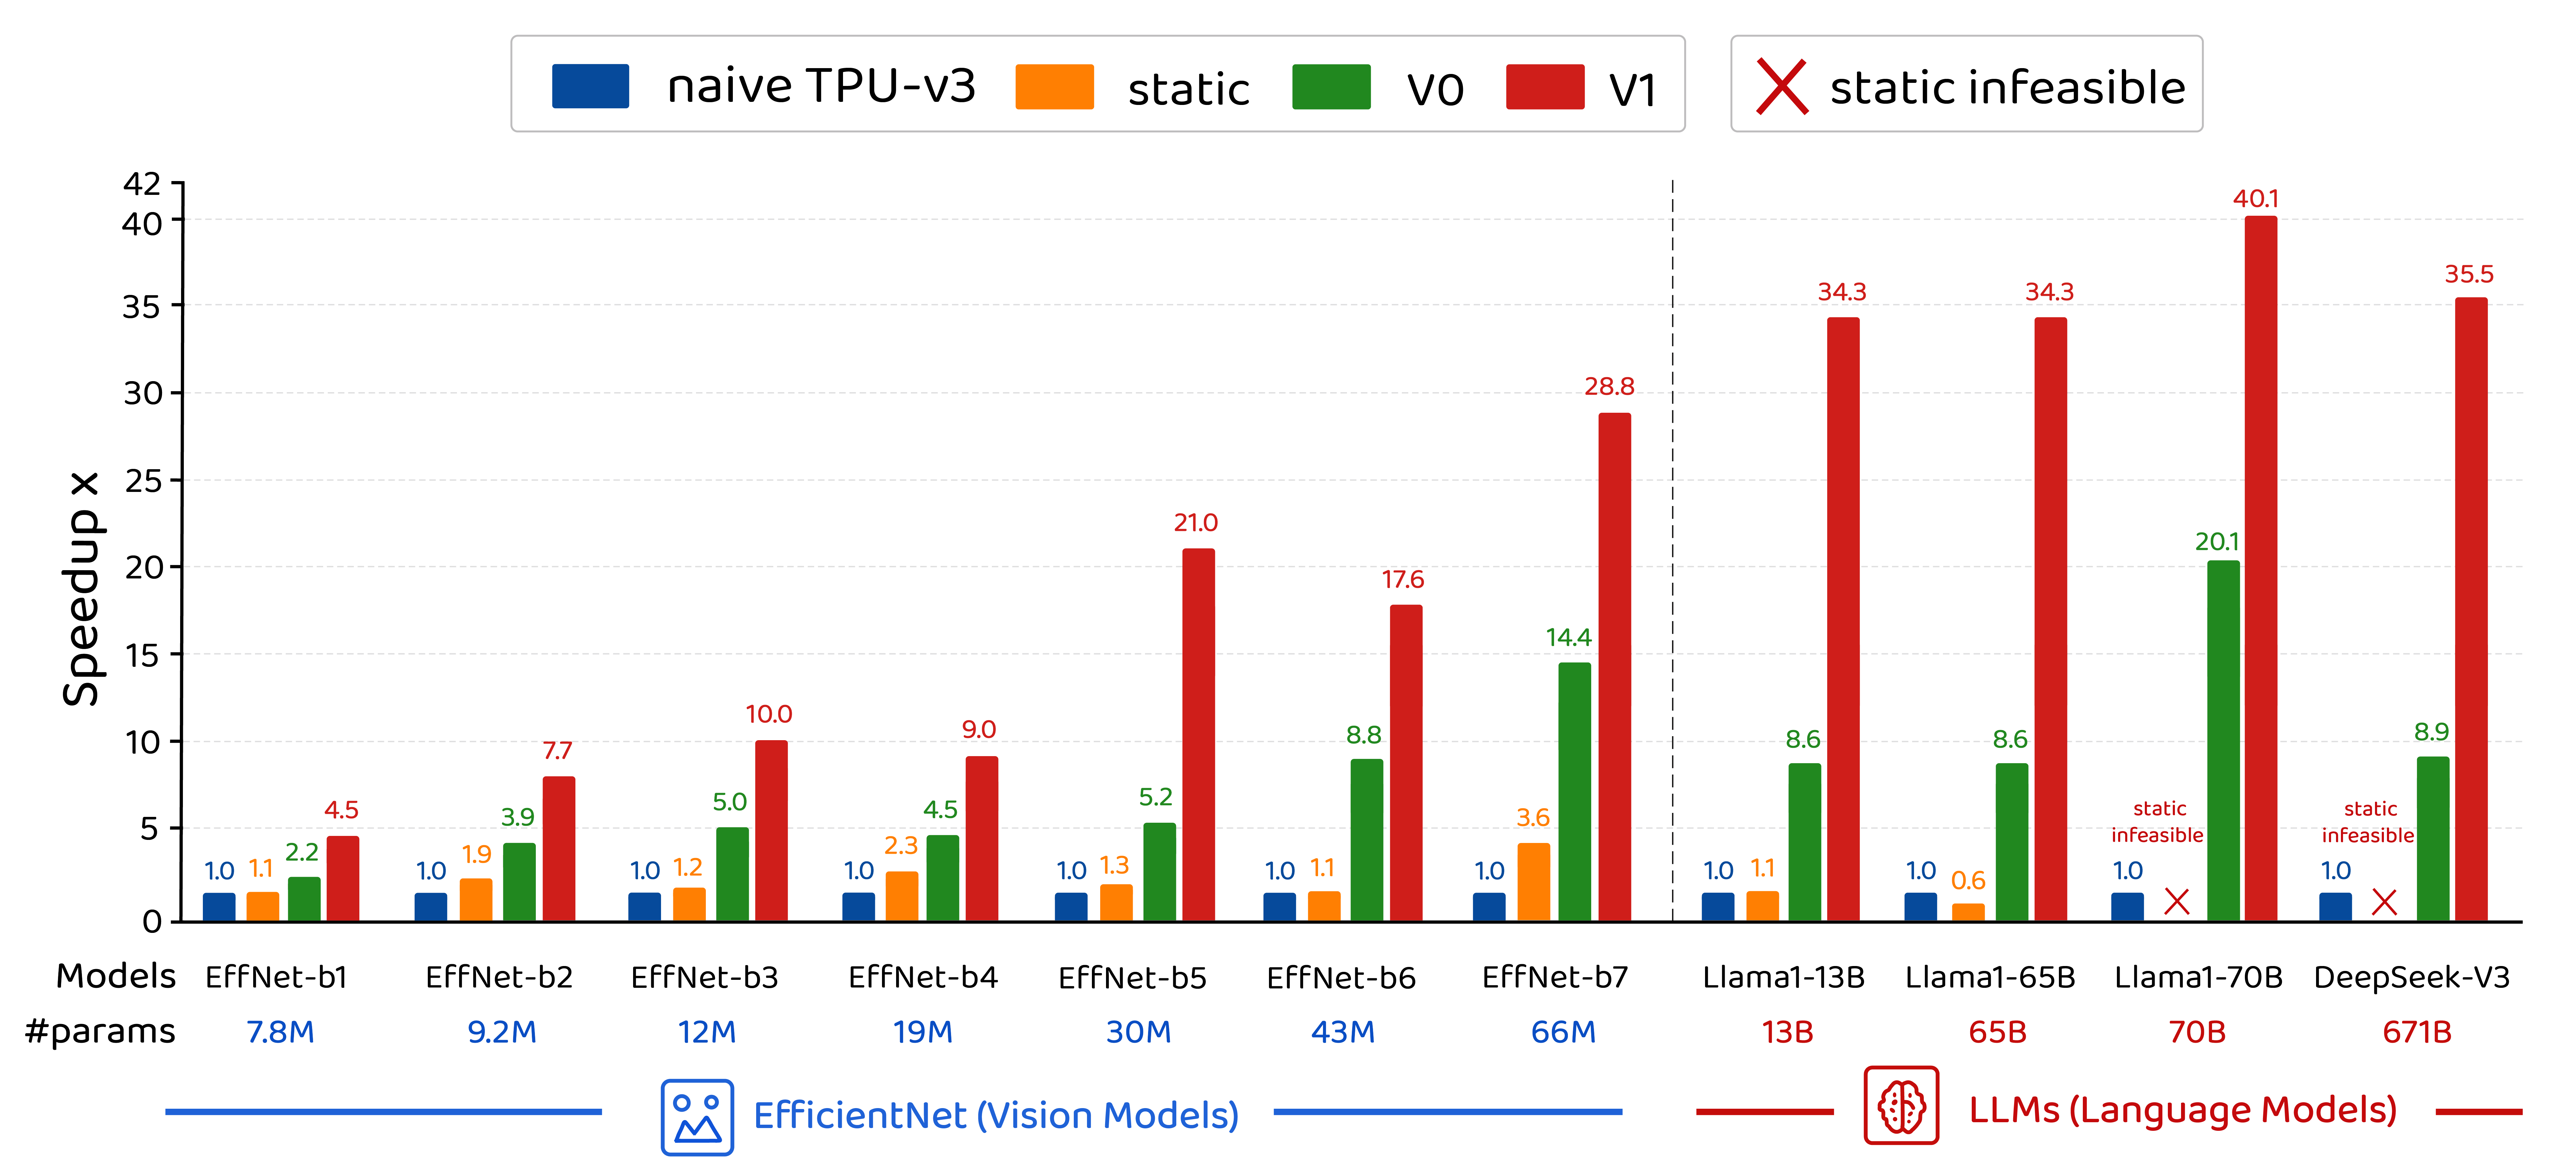
\includegraphics[width=1.0\linewidth]{fig3/speedup_final_v2.png}
% % \caption{Speedup over modeled TPU-v3 baseline across formulations and workloads: CHEETAH-V1's joint tiling-fusion optimization achieves up to $\sim$35× acceleration, while static fusion is infeasible on large-scale LLMs.}
% % \label{fig:speedup}
% % \end{figure}

% % % In addition to efficiently enabling more globally optimized accelerator designs, we anticipate that future work may build off this foundation to implement custom Flash Attention type speedup mechanisms for individual hardware (such as RTX5090) and workloads (such as LLama70B) tractably within hours, as well as quickly and efficiently design custom accelerators for targeted inference tasks. 
% % % compromise on any single workload; a growing body of evidence suggests that workload-specialized designs can deliver $2$--$6\times$ improvements in performance per watt.
% % % The resulting system replaces FAST's sequential Timeloop$\rightarrow$fusion~ILP pipeline with a single LP that jointly optimizes tiling, fusion, and memory scheduling, while preserving Vizier's outer loop over hardware configurations (or replacing it with LLM-guided search).

% % % Furthermore, FAST's fusion ILP uses static tensor placement: a tensor is either pinned for the entire inference pass or not at all.
% % % This is overly conservative for models with long dependency chains or skip connections, where different tensors are live at different times during execution.
% % % A dynamic placement strategy that can evict and re-pin tensors across timesteps could substantially improve global memory utilization. Joint Optimization is the only way to solve the "Memory Wall" for large scale models like DeepSeek-V3.

% % % FAST operates via a three-stage sequential pipeline (Figure \ref{fig::workflow}): (1)~a black-box optimizer (Google Vizier \citep{google_vizier}) proposes a hardware configuration defined by 16 hyperparameters---PE grid dimensions, systolic array sizes, buffer capacities, DRAM channels, and batch size; (2)~a scheduling engine (Timeloop \citep{timeloop}) finds the best tiling and mapping for each operation independently given the fixed hardware; and (3)~an integer linear program (ILP) decides which tensors to pin in the on-chip Global Memory to reduce DRAM traffic.
% % % The result of each trial---predicted performance per TDP---is fed back to Vizier, which proposes the next hardware configuration, repeating for thousands of trials until convergence.


% % % automate the framework with SkyDiscover Loop for profile and context aware co-design. Therefore in less than five hours, we are able to find an more performant design spec than the strongest baseline on designing , in terms of both perf/TDP and speedup. Our experiments also include freezing any hardware at input, and reducing the scheduling, tiling, etc search to just the LP can yield speedups of avg 2.2x than just the base hardware along. We anticipate that future work may build off this foundation to implement custom Flash Attention type speedup mechanisms for individual hardware (such as RTX5090) and workloads (such as LLama70B) tractably within hours. 

% % % Our propose the formulation for global co-design for a custom accelerator as a large scale linear program which captures strict dependencies and tradeoffs sequential methods may miss. Our LP formulation captures scheduling, tiling, rematerialization, and is able to solve matrices at scales of $6{,}319 \times 4{,}516$,\ nnz$=829{,}852$ \& $3{,}669{,}793 \times 3{,}263{,}443$,\ nnz$=7{,}342{,}293$ \& $2{,}983{,}450 \times 2{,}504{,}019$,\ nnz$=6{,}094{,}156$ quickly, by utilizing a JAX based large scale solver. Our insight is that despite the challenging large scale of the problem, the structure of the matrices, once formed, retain the same structure. Therefore we are able to design one preconditioning scheme to these large scale systems matrices that can be re-used across any NN. This also allows us to capture dependencies prior methods cannot, for example our formulation introduces a dynamic placement strategy that can evict and re-pin tensors across timesteps could substantially improve global memory utilization. Joint Optimization is the only way to solve the "Memory Wall" for large scale models like DeepSeek-V3. 

% % % For EfficientNet-B7 at $L=400$ operations and $T=400$ timesteps, the V1 LP contains approximately $2$ million variables and $5$ million constraints with $15$--$25$ million nonzeros. To better solve such large-scale LP problems more efficiently, we implement our own variant of a GPU-accelerated solver based on recent primal-dual LP algorithm \citep{applegate2022practicallargescalelinearprogramming}. We extend its original formulation in various ways and benchmark our implementation compared to existing commercial SciPy solvers, which showcase the advantage of our solver. To keep the main context clean and focused, we defer LP solver-related details to Appendix \ref{app:solver}.

% % % A large number of black box optimization tools to handle this large search space have been recently proposed, such as Google's Vizier, Meta's AX, and Optuna. In addition search strategies are also explored, for example Google's Vizier proposes numerous methods Gaussian Process Upper Confidence Bound, Eagle Strategy as a metaheuristic optimization algorithm designed for global optimization via a two-stage hybrid approach that combines global exploration with intensive local search, and Linear Combination Swarm (LCS). However these methods share certain limitations, since they cannot globally capture the tradeoffs and tensions between sequential decisions and rely on brute force iterations. This requires human engineers to spend months of compute and thousands of repetitive trials to get improvements, without feedback on what might be globally optimal. 

% % % While this sequential decomposition makes the problem tractable, it introduces a fundamental limitation: \emph{each stage takes the previous stage's output as fixed input, preventing the discovery of solutions that require trading off across stages.} Consider a concrete example: for a depthwise-separable convolution layer in a NN, a search tool such as Timeloop might select a tiling configuration that maximizes compute utilization at $74\%$, producing an activation working set of $6$ MiB. THe stacked The downstream fusion ILP solver tool receives this fixed working set size, cannot fit the tensor into the $128$ MiB Global Memory alongside other pinned tensors. However, an alternative tiling configuration with slightly lower utilization ($70\%$) might produce a working set of only $3$ MiB, enabling the fusion solver to pin an additional weight tensor that eliminates a DRAM bottleneck entirely, thus yielding a net $>20\%$ cycle reduction despite the $4\%$ utilization loss. Therefore these sequential pipelines systematically misses such cross-stage trade-offs.

% % % The rapid evolution of deep learning workloads has created a compelling opportunity for domain-optimized inference accelerators.
% % % Production models now serve billions of daily users, and the computational demands of architectures based on depthwise-separable convolutions (EfficientNet), self-attention (BERT, LLaMA), mixture-of-experts (DeepSeek-V3, Mixtral), and state-space models (Mamba) differ dramatically in their compute-to-memory ratios, tensor shapes, and data reuse patterns. However although the NN training strategy has been scaled up and we've done a lot of work on it, we now face the inference bottle neck era since general-purpose hardware, Nvidia's gaming GPUs are not necessarily optimized for deep learning tasks, and leaves a huge amount of compute on the table.


% % page edit

% \section{Introduction}
% \label{sec:introduction}

% \begin{figure}[ht!]
%     \centering
%     \includegraphics[width=1.0\linewidth]{figs/cheetah_v4.png}
%     % \caption{\textbf{FAST vs.\ FAST-CORGI pipeline comparison.} 
% \caption{Sequential vs Our Unified Optimization Paradigm.
% (Left) Baseline methods decouple hardware search, operation-level tiling, and static fusion; precluding cross-stage trade-offs.
% (Right) CHEETAH presents a unified LLM-driven LP-solver-based framework that jointly optimizes tiling, placement, and rematerialization while learning from a causal ledger.}
% \label{fig::workflow}
% \end{figure}
% % The rapid evolution of deep learning workloads varies from convolutions to self-attention (LLaMA), mixture-of-experts (DeepSeek-V3), and state-space models (Mamba). These diverse architectures serve billions of daily users, and have fundamentally shifted the requirements for hardware acceleration. As foundation models continue to scale in parameters, the primary cost and bottleneck of model deployment has shifted from training to inference. Therefore much recent research has been focused on optimizing for more efficient execution and throughput across diverse, high-dimensional workloads. General-purpose GPUs remain largely designed for graphics-heavy throughput, and leave substantial efficiency and compute on the table at these tasks. Therefore we are motivated to design targeted accelerators that are optimized for handling the varying tensor shapes and data-reuse patterns of modern deep learning architectures.
% % Much research has been done in accelerating inference through custom accelerator design, more efficient neural network (NN) batching algorithms, and domain specific packages and languages that aim to speed up general NN inference. For example, the widely adopted Flash Attention uses tiling to provide significant speedups by optimizing memory movement between SRAM and DRAM. Co-design takes this a step further by aiming to optimize hardware, software and scheduling to unlock performance neither could reach independently. The traditional framework of doing this is a sequential pipeline of heuristics tools, requiring human engineers to iterate through a large search space for months from testing for the size of DRAM, to determining higher level scheduling problems. Optimizing each piece of this complex pipeline is extremely challenging, since hardware datapaths, software schedules, and compiler transforms across a combinatorial space exceeding $\mathcal O(10^{2300})$.
% The AI inference demand is expected to grow by $10,000\times$ over the next 5 years \citep{cra2026aifuture}. General-purpose accelerators leave significant efficiency gains unrealized, which motivates the design of targeted custom accelerators. Co-design, which jointly optimizes hardware-software (HW/SW), and scheduling for target workloads, offers a path to unlock performance efficiency for the upcoming inference era. However, the prevailing approach relies on sequential pipelines of heuristic tools, a slow, human-driven process navigating a combinatorial search space exceeding $O(10^{2300})$ \citep{zhang_fast}. State-of-the-art frameworks like FAST \citep{zhang_fast} improve on this through an automated flow (a hardware proposer feeds an operation-level tiling agent, which feeds a downstream fusion solver), but remain fundamentally decoupled: a tiling that slightly reduces compute efficiency may shrink the working set enough to eliminate a DRAM bottleneck, yet sequential pipelines cannot discover such cross-stage trade-offs.

% % The co-design problem is increasingly important as inference efficiency is the dominant AI workload and is rapidly growing. Therefore industry leaders such as NVIDIA and Google have designed chips for improved hardware-native agentic AI and , and state-of-the-art frameworks such as FAST, address this through a sequential decomposition of heuristics (a hardware proposer feeds an operation-level tiling agent, which feeds a downstream fusion solver). While FAST-generated accelerators can provide increased speedups over baseline TPU-v3, this decoupled approach is limited since it cannot capture cross-stage trade-offs. A tiling configuration that is \textit{locally} optimal for one layer may create an activation footprint that later prevents \textit{global} fusion, while a slightly slower tiling might shrink the working set enough to eliminate a DRAM bottleneck entirely. Sequential pipelines are systematically unable to express these interactions, leading to locally good but globally sub-optimal designs. 
% Unifying the design space into a single convex relaxation yields previously infeasible global optima. Specifically, we introduce CHEETAH: a custom inference accelerator design framework that unlocks globally optimized designs with a dual-loop. Our inner-loop is a novel large-scale Linear Program (LP) to precisely mathematically model strict design decisions and constraints that must not be violated. The LP captures trade-offs for targeted workloads through time-indexed placement and rematerialization, thus allowing tensors to be dynamically pinned, evicted, recomputed across inference timesteps. We further extend our reformulation to internalize tiling selection into the LP, by introducing Pareto-pruned tiling variables and the McCormick linearization (a convex relaxation used for optimization of bilinear problems \citep{mccormick1976computability}). By exploiting the structural invariance of our matrices across hardware trials, we also adapt a GPU-accelerated primal-dual solver in JAX \citep{jax2018github} that can resolve millions of variables to rapidly reduce trial time from days to hours. This allows the LP solver to jointly reason about hardware configuration, activation placement, and weight pinning in a single pass, while providing feedback signal via Lagrangian duals.

% Our outer-loop framework stacks a black-box optimizer (Google Vizier \citep{google_vizier}) to propose candidate hardware configurations defined by a set of hyperparameters (e.g., processing element grid dimensions, systolic array sizes, DRAM size, etc), while a LLM is used for efficient search-space steering. The LLM acts as a causal architect, interpreting a compact trial ledger of roofline checks and LP feedback diagnostics to propose constrained architectural search input for Vizier. This prevents the search-space gaming typical of black-box optimizers in wide design regions, and reduces the need for thousands of sequential trials via Bayesian search strategies in Vizier to learn good vs bad neighborhoods in search topology. Our results demonstrate that the LLM Architect framework further reduces invalid hardware trials from 24.5\% under vanilla Vizier to 5.9\%, while reaching the Pareto frontier 4.5x faster than the next strongest baseline. We validate all results with Model Flop Utilization (MFU) and roofline lower-bound audits, ensuring predicted latencies are physically grounded in compute and memory throughput limits. 
% % \todo{Add best of both worlds, strengths from principled LP side, from LLM aggregate info side}
% % \todo{Aggregates past experience to gain insight into steering hardware-software co-design. We offload the strict solves, with constraints that must the strictly respected, to the LP solve part. This combines the best of both worlds.} 
% \paragraph{Contributions.} We reformulated the fundamental HW/SW co-design problem into a unified  framework in CHEETAH, combining principled mathematical rigor of the LP formulation to solve strict design decisions optimally, with the powerful aggregation and causal learning of an LLM Architect outer loop for meta-optimization. Our open-source repository for full reproducibility is at \href{https://anonymous.4open.science/r/CHEETAH-B268/readme}{https://anonymous.4open.science/r/CHEETAH-B268/}.

% \begin{enumerate}
%     \item \textbf{CHEETAH-V0 - Dynamic Placement with Rematerialization:}
%     We introduce time-indexed LP variables $p_{i,t}^k$ and rematerialization variables $r_{i,t}$ to enable cheap recompute operations instead of paying DRAM reload costs, supporting skip connections and multi-fanout nodes.

%     \item \textbf{CHEETAH-V1 - Joint Tiling-Fusion:}
%     We unify tiling and fusion into a single LP problem by introducing tiling selection variables $y_{i,c}$, and employ McCormick envelopes to exactly linearize the bilinear interaction between tiling and tensor pinning. This technique yields a tight, parameter-free LP relaxation, and the coupling internalizes the tiling-placement trade-off to discover optimal design points that sequential pipelines systematically miss.
%     % This enables the LP to discover trade-offs where accepting a suboptimal tiling configuration enables superior fusion, or vice versa---precisely the cross-stage interactions that the sequential pipeline cannot capture.
%     \item \textbf{LLM-guided Causal Architect:} The LLM outer loop steers hardware search by interpreting Lagrangian sensitivity signals and a Causal Ledger of past trials to perform targeted subspace interventions, transforming black-box search into a structured, diagnostic-driven process. The Architect guides Vizier through widened search spaces, reducing invalid trials by ${\sim}4\times$ while preserving the global optimal score, and enables profile-specific designs (speech models may emphasize latency, while data synthesis models may prioritize bandwidth). 
%     \item \textbf{Speedup:} Our method demonstrates an average speedup of $\sim22.07\times$ over the baseline across a wide range of $11$ vision and language models, reaching up to ${\sim}40.1\times$ on a single workload, as shown in  Figure \ref{fig:speedup} below.

%     % profiles into consideration to push the black-box optimizer responsible for hardware suggestions to output with structured reasoning about architectural trade-offs. 

% \end{enumerate}

% \begin{figure}[ht!]
%     \centering
% 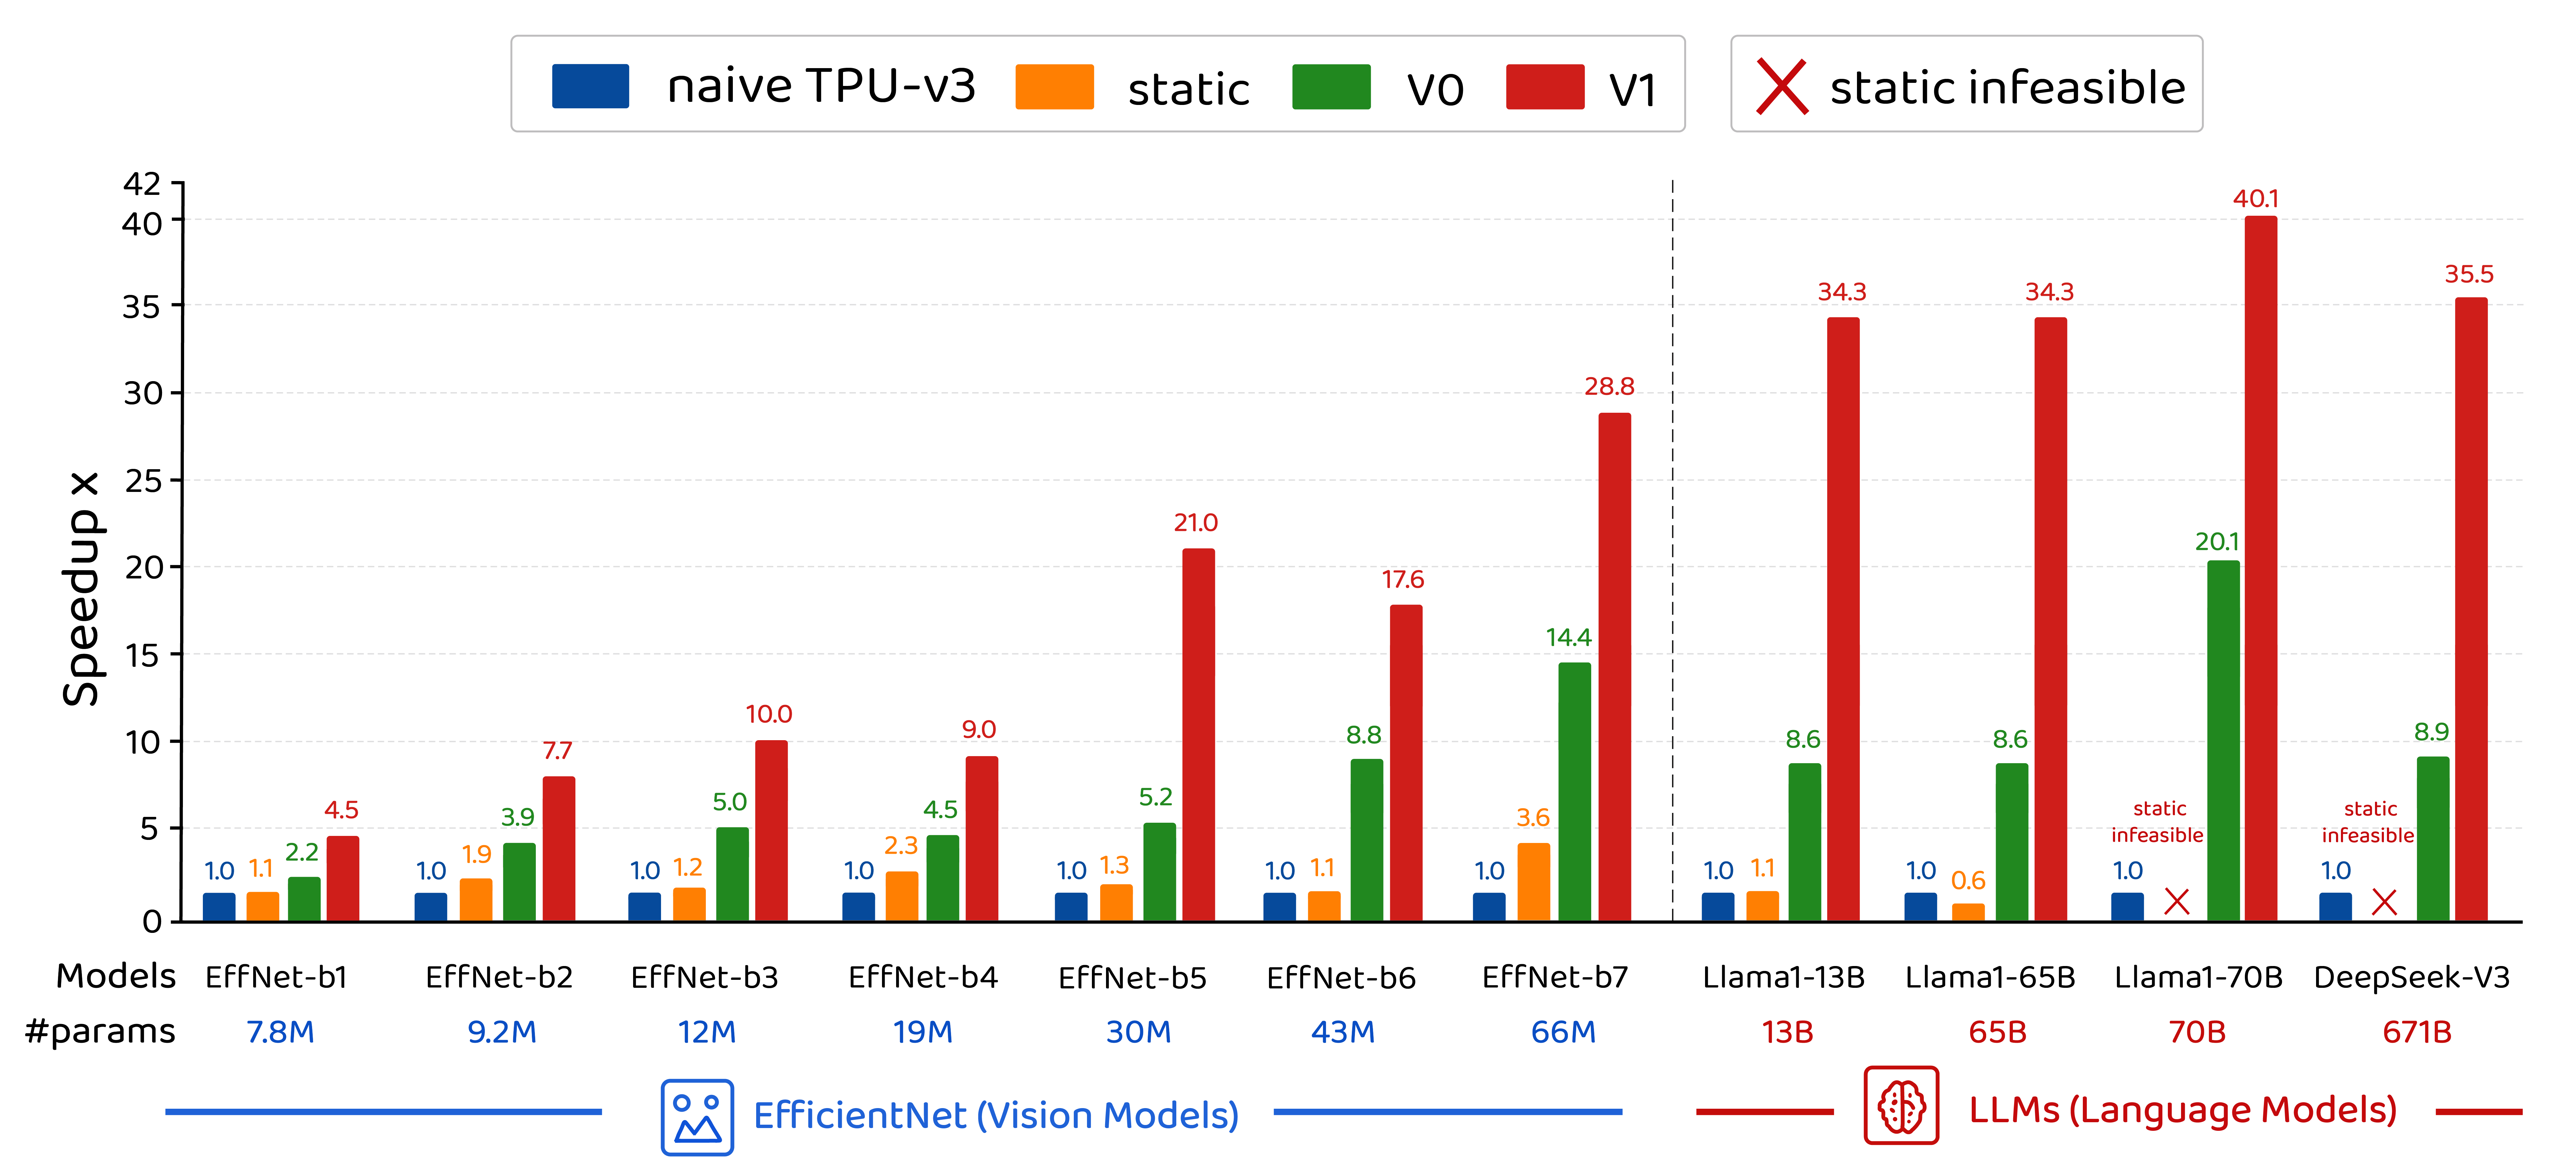
\includegraphics[width=1.0\linewidth]{fig3/speedup_final_v2.png}
% \caption{Speedup over modeled TPU-v3 baseline across formulations and workloads: CHEETAH-V1's joint tiling-fusion optimization achieves up to $\sim$40.1$\times$ acceleration, while static fusion is infeasible on large-scale LLMs. Progressive gains are visible across formulations: V0's dynamic placement improves over static by $2$--$20\times$, while V1's joint tiling-fusion adds another $2$--$4\times$ on top. See Section~\ref{sec:experiments} for full analysis and wall-clock time breakdowns.}
% \label{fig:speedup}
% \end{figure}

% % In addition to efficiently enabling more globally optimized accelerator designs, we anticipate that future work may build off this foundation to implement custom Flash Attention type speedup mechanisms for individual hardware (such as RTX5090) and workloads (such as LLama70B) tractably within hours, as well as quickly and efficiently design custom accelerators for targeted inference tasks. 
% % compromise on any single workload; a growing body of evidence suggests that workload-specialized designs can deliver $2$--$6\times$ improvements in performance per watt.
% % The resulting system replaces FAST's sequential Timeloop$\rightarrow$fusion~ILP pipeline with a single LP that jointly optimizes tiling, fusion, and memory scheduling, while preserving Vizier's outer loop over hardware configurations (or replacing it with LLM-guided search).

% % Furthermore, FAST's fusion ILP uses static tensor placement: a tensor is either pinned for the entire inference pass or not at all.
% % This is overly conservative for models with long dependency chains or skip connections, where different tensors are live at different times during execution.
% % A dynamic placement strategy that can evict and re-pin tensors across timesteps could substantially improve global memory utilization. Joint Optimization is the only way to solve the "Memory Wall" for large scale models like DeepSeek-V3.

% % FAST operates via a three-stage sequential pipeline (Figure \ref{fig::workflow}): (1)~a black-box optimizer (Google Vizier \citep{google_vizier}) proposes a hardware configuration defined by 16 hyperparameters---PE grid dimensions, systolic array sizes, buffer capacities, DRAM channels, and batch size; (2)~a scheduling engine (Timeloop \citep{timeloop}) finds the best tiling and mapping for each operation independently given the fixed hardware; and (3)~an integer linear program (ILP) decides which tensors to pin in the on-chip Global Memory to reduce DRAM traffic.
% % The result of each trial---predicted performance per TDP---is fed back to Vizier, which proposes the next hardware configuration, repeating for thousands of trials until convergence.


% % automate the framework with SkyDiscover Loop for profile and context aware co-design. Therefore in less than five hours, we are able to find an more performant design spec than the strongest baseline on designing , in terms of both perf/TDP and speedup. Our experiments also include freezing any hardware at input, and reducing the scheduling, tiling, etc search to just the LP can yield speedups of avg 2.2x than just the base hardware along. We anticipate that future work may build off this foundation to implement custom Flash Attention type speedup mechanisms for individual hardware (such as RTX5090) and workloads (such as LLama70B) tractably within hours. 

% % Our propose the formulation for global co-design for a custom accelerator as a large scale linear program which captures strict dependencies and tradeoffs sequential methods may miss. Our LP formulation captures scheduling, tiling, rematerialization, and is able to solve matrices at scales of $6{,}319 \times 4{,}516$,\ nnz$=829{,}852$ \& $3{,}669{,}793 \times 3{,}263{,}443$,\ nnz$=7{,}342{,}293$ \& $2{,}983{,}450 \times 2{,}504{,}019$,\ nnz$=6{,}094{,}156$ quickly, by utilizing a JAX based large scale solver. Our insight is that despite the challenging large scale of the problem, the structure of the matrices, once formed, retain the same structure. Therefore we are able to design one preconditioning scheme to these large scale systems matrices that can be re-used across any NN. This also allows us to capture dependencies prior methods cannot, for example our formulation introduces a dynamic placement strategy that can evict and re-pin tensors across timesteps could substantially improve global memory utilization. Joint Optimization is the only way to solve the "Memory Wall" for large scale models like DeepSeek-V3. 

% % For EfficientNet-B7 at $L=400$ operations and $T=400$ timesteps, the V1 LP contains approximately $2$ million variables and $5$ million constraints with $15$--$25$ million nonzeros. To better solve such large-scale LP problems more efficiently, we implement our own variant of a GPU-accelerated solver based on recent primal-dual LP algorithm \citep{applegate2022practicallargescalelinearprogramming}. We extend its original formulation in various ways and benchmark our implementation compared to existing commercial SciPy solvers, which showcase the advantage of our solver. To keep the main context clean and focused, we defer LP solver-related details to Appendix \ref{app:solver}.

% % A large number of black box optimization tools to handle this large search space have been recently proposed, such as Google's Vizier, Meta's AX, and Optuna. In addition search strategies are also explored, for example Google's Vizier proposes numerous methods Gaussian Process Upper Confidence Bound, Eagle Strategy as a metaheuristic optimization algorithm designed for global optimization via a two-stage hybrid approach that combines global exploration with intensive local search, and Linear Combination Swarm (LCS). However these methods share certain limitations, since they cannot globally capture the tradeoffs and tensions between sequential decisions and rely on brute force iterations. This requires human engineers to spend months of compute and thousands of repetitive trials to get improvements, without feedback on what might be globally optimal. 

% % While this sequential decomposition makes the problem tractable, it introduces a fundamental limitation: \emph{each stage takes the previous stage's output as fixed input, preventing the discovery of solutions that require trading off across stages.} Consider a concrete example: for a depthwise-separable convolution layer in a NN, a search tool such as Timeloop might select a tiling configuration that maximizes compute utilization at $74\%$, producing an activation working set of $6$ MiB. THe stacked The downstream fusion ILP solver tool receives this fixed working set size, cannot fit the tensor into the $128$ MiB Global Memory alongside other pinned tensors. However, an alternative tiling configuration with slightly lower utilization ($70\%$) might produce a working set of only $3$ MiB, enabling the fusion solver to pin an additional weight tensor that eliminates a DRAM bottleneck entirely, thus yielding a net $>20\%$ cycle reduction despite the $4\%$ utilization loss. Therefore these sequential pipelines systematically misses such cross-stage trade-offs.

% % The rapid evolution of deep learning workloads has created a compelling opportunity for domain-optimized inference accelerators.
% % Production models now serve billions of daily users, and the computational demands of architectures based on depthwise-separable convolutions (EfficientNet), self-attention (BERT, LLaMA), mixture-of-experts (DeepSeek-V3, Mixtral), and state-space models (Mamba) differ dramatically in their compute-to-memory ratios, tensor shapes, and data reuse patterns. However although the NN training strategy has been scaled up and we've done a lot of work on it, we now face the inference bottle neck era since general-purpose hardware, Nvidia's gaming GPUs are not necessarily optimized for deep learning tasks, and leaves a huge amount of compute on the table.



% figure 2 reference edit again

% \section{Introduction}
% \label{sec:introduction}

% \begin{figure}[ht!]
%     \centering
%     \includegraphics[width=1.0\linewidth]{figs/cheetah_v4.png}
% \caption{Sequential vs Unified Optimization Paradigm Comparison.
% (Left) Baseline methods decouple hardware search, operation-level tiling, and static fusion; precluding cross-stage trade-offs.
% (Right) CHEETAH presents a unified LLM-driven LP-solver-based framework that jointly optimizes tiling, placement, and rematerialization while learning from a causal ledger.}
% \label{fig::workflow}
% \end{figure}
% % The rapid evolution of deep learning workloads varies from convolutions to self-attention (LLaMA), mixture-of-experts (DeepSeek-V3), and state-space models (Mamba). These diverse architectures serve billions of daily users, and have fundamentally shifted the requirements for hardware acceleration. As foundation models continue to scale in parameters, the primary cost and bottleneck of model deployment has shifted from training to inference. Therefore much recent research has been focused on optimizing for more efficient execution and throughput across diverse, high-dimensional workloads. General-purpose GPUs remain largely designed for graphics-heavy throughput, and leave substantial efficiency and compute on the table at these tasks. Therefore we are motivated to design targeted accelerators that are optimized for handling the varying tensor shapes and data-reuse patterns of modern deep learning architectures.
% % Much research has been done in accelerating inference through custom accelerator design, more efficient neural network (NN) batching algorithms, and domain specific packages and languages that aim to speed up general NN inference. For example, the widely adopted Flash Attention uses tiling to provide significant speedups by optimizing memory movement between SRAM and DRAM. Co-design takes this a step further by aiming to optimize hardware, software and scheduling to unlock performance neither could reach independently. The traditional framework of doing this is a sequential pipeline of heuristics tools, requiring human engineers to iterate through a large search space for months from testing for the size of DRAM, to determining higher level scheduling problems. Optimizing each piece of this complex pipeline is extremely challenging, since hardware datapaths, software schedules, and compiler transforms across a combinatorial space exceeding $\mathcal O(10^{2300})$.
% The AI inference demand is expected to grow by $10,000\times$ over the next 5 years \citep{cra2026aifuture}. General-purpose accelerators leave significant efficiency gains unrealized, which motivates the design of targeted custom accelerators. Co-design, which jointly optimizes hardware, software, and scheduling for target workloads, offers a path to unlock performance efficiency for the upcoming inference era. However, the prevailing approach relies on sequential pipelines of heuristic tools, a slow, human-driven process navigating a combinatorial search space exceeding $O(10^{2300})$ \citep{zhang_fast}. State-of-the-art frameworks like FAST \citep{zhang_fast} improve on through an automated flow (a hardware proposer feeds an operation-level tiling agent, which feeds a downstream fusion solver), but remain fundamentally decoupled.  For example, a tiling configuration that is \textit{locally} optimal for one layer may create an activation footprint that later prevents \textit{global} fusion, while a slightly slower tiling might shrink the working set enough to eliminate a DRAM bottleneck entirely. Sequential pipelines are systematically unable to express these interactions, leading to locally good but globally sub-optimal designs.

% % The co-design problem is increasingly important as inference efficiency is the dominant AI workload and is rapidly growing. Therefore industry leaders such as NVIDIA and Google have designed chips for improved hardware-native agentic AI and , and state-of-the-art frameworks such as FAST, address this through a sequential decomposition of heuristics (a hardware proposer feeds an operation-level tiling agent, which feeds a downstream fusion solver). While FAST-generated accelerators can provide increased speedups over baseline TPU-v3, this decoupled approach is limited since it cannot capture cross-stage trade-offs. A tiling configuration that is \textit{locally} optimal for one layer may create an activation footprint that later prevents \textit{global} fusion, while a slightly slower tiling might shrink the working set enough to eliminate a DRAM bottleneck entirely. Sequential pipelines are systematically unable to express these interactions, leading to locally good but globally sub-optimal designs. 
% We prove that by unifying the design space into a single convex relaxation, we find global optima that were previously  infeasible. Specifically, we introduce CHEETAH: a custom inference accelerator design framework that unlocks globally optimized designs with a dual-loop engine (See Figure \ref{fig::workflow}). Our inner-loop is a novel large-scale Linear Program (LP) to precisely mathematically model strict design decisions and constraints that must not be violated. The LP captures trade-offs for targeted workloads through time-indexed placement and rematerialization, thus allowing tensors to be dynamically pinned, evicted, recomputed across inference timesteps. We further extend our reformulation to internalize tiling selection into the LP, by introducing Pareto-pruned tiling variables and the McCormick linearization (a convex relaxation used for optimization of bilinear problems \citep{mccormick1976computability}). By exploiting the structural invariance of our matrices across hardware trials, we also adapt a GPU-accelerated primal-dual solver in JAX that can resolve millions of variables to rapidly reduce trial time from days to hours. This allows the LP solver to jointly reason about hardware configuration, activation placement, and weight pinning in a single pass, while providing feedback signal via Lagrangian duals.

% Our outer-loop framework stacks a black-box optimizer (Google Vizier \citep{google_vizier}) to propose candidate hardware configurations defined by a set of hyperparameters (e.g., processing element grid dimensions, systolic array sizes, DRAM size, etc), while a LLM is used for efficient search-space steering. The LLM acts as a causal architect, interpreting a compact trial ledger of roofline checks and LP feedback diagnostics to propose constrained architectural search input for Vizier. This prevents the search-space gaming typical of black-box optimizers in wide design regions, and reduces the need for thousands of sequential trails via Bayesian search strategies in Vizier to learn good vs bad neighborhoods in search topology. Our results demonstrate that the LLM-Architect framework further reduces invalid hardware trials from 24.5\% under vanilla Vizier to 5.9\%, while reaching the Pareto frontier 4.5x faster than the next strongest baseline. We validate all results with Model Flop Utilization (MFU)  and roofline lower-bound audits, ensuring predicted latencies are physically grounded in compute and memory throughput limits. 
% % \todo{Add best of both worlds, strengths from principled LP side, from LLM aggregate info side}
% % \todo{Aggregates past experience to gain insight into steering hardware-software co-design. We offload the strict solves, with constraints that must the strictly respected, to the LP solve part. This combines the best of both worlds.} 
% \paragraph{Contributions.} We reformulated the fundamental HW/SW co-design problem into a unified  framework in CHEETAH, combining principled mathematical rigor of the LP formulation to solve strict design decisions optimally, with the powerful aggregation and causal learning of an LLM Architect outer loop for meta-optimization. Our open-source repository for full reproducibility is at \href{https://anonymous.4open.science/r/CHEETAH-B268/readme}{https://anonymous.4open.science/r/CHEETAH-B268/}.

% \begin{enumerate}
%     \item \textbf{CHEETAH-V0 - Dynamic Placement with Rematerialization:}
%     We introduce the time-indexed and rematerialization variables to enable cheap recompute operations (\eg, depthwise convolutions that account for only $5\%$ of FLOPs but produce large activations) instead of paying DRAM reload costs. This addresses the restrictions of existing baseline methods where activations can only be pinned between consecutively-executed operations, and supports skip connections and multi-fanout nodes.

%     \item \textbf{CHEETAH-V1 - Joint Tiling-Fusion:}
%     We unify tiling and fusion into a single LP problem by introducing tiling selection variables $y_{i,c}$, and employ McCormick envelopes to exactly linearize the bilinear interaction between tiling and tensor pinning. This technique yields a tight, parameter-free LP relaxation, and the coupling internalizes the tiling-placement trade-off to discover optimal design points that sequential pipelines systematically miss.
%     % This enables the LP to discover trade-offs where accepting a suboptimal tiling configuration enables superior fusion, or vice versa---precisely the cross-stage interactions that the sequential pipeline cannot capture.
%     \item \textbf{LLM-guided Causal Architect:} The LLM outer loop steers hardware search and bridges high-level architectural reasoning with low-level solver duals. It interprets Lagrangian sensitivity signals to perform targeted subspace interventions, transforming black-box search into a structured, diagnostic-driven process. We use a context-aware LLM Architect to propose good search areas as input to Vizier (a black-box Bayesian optimizer). Feedback signals are aggregated across historical trials through both the Causal Ledger and the LP solver. The Architect then guides Vizier through widened search spaces, reducing invalid trials by ${\sim}4\times$ while preserving the global optimal score, while enabling profile-specific designs (speech models may emphasize latency, while data synthesis models may prioritize bandwidth). 
%     \item \textbf{Speedup:} We show that across a large suite of vision and language modeling workloads, CHEETAH results in an average of 20.9X faster designs than prior work. 

%     % profiles into consideration to push the black-box optimizer responsible for hardware suggestions to output with structured reasoning about architectural trade-offs. 

% \end{enumerate}

% We anticipate that future work may build from this framework in two ways: as an end-to-end co-design system for efficient accelerators, and as an automated optimization engine for existing hardware. By fixing the architecture, the inner loop derives optimal tiling and scheduling strategies that can act as custom speedups for targeted inference tasks.

% % \begin{figure}[ht!] 
% %     \centering
% % 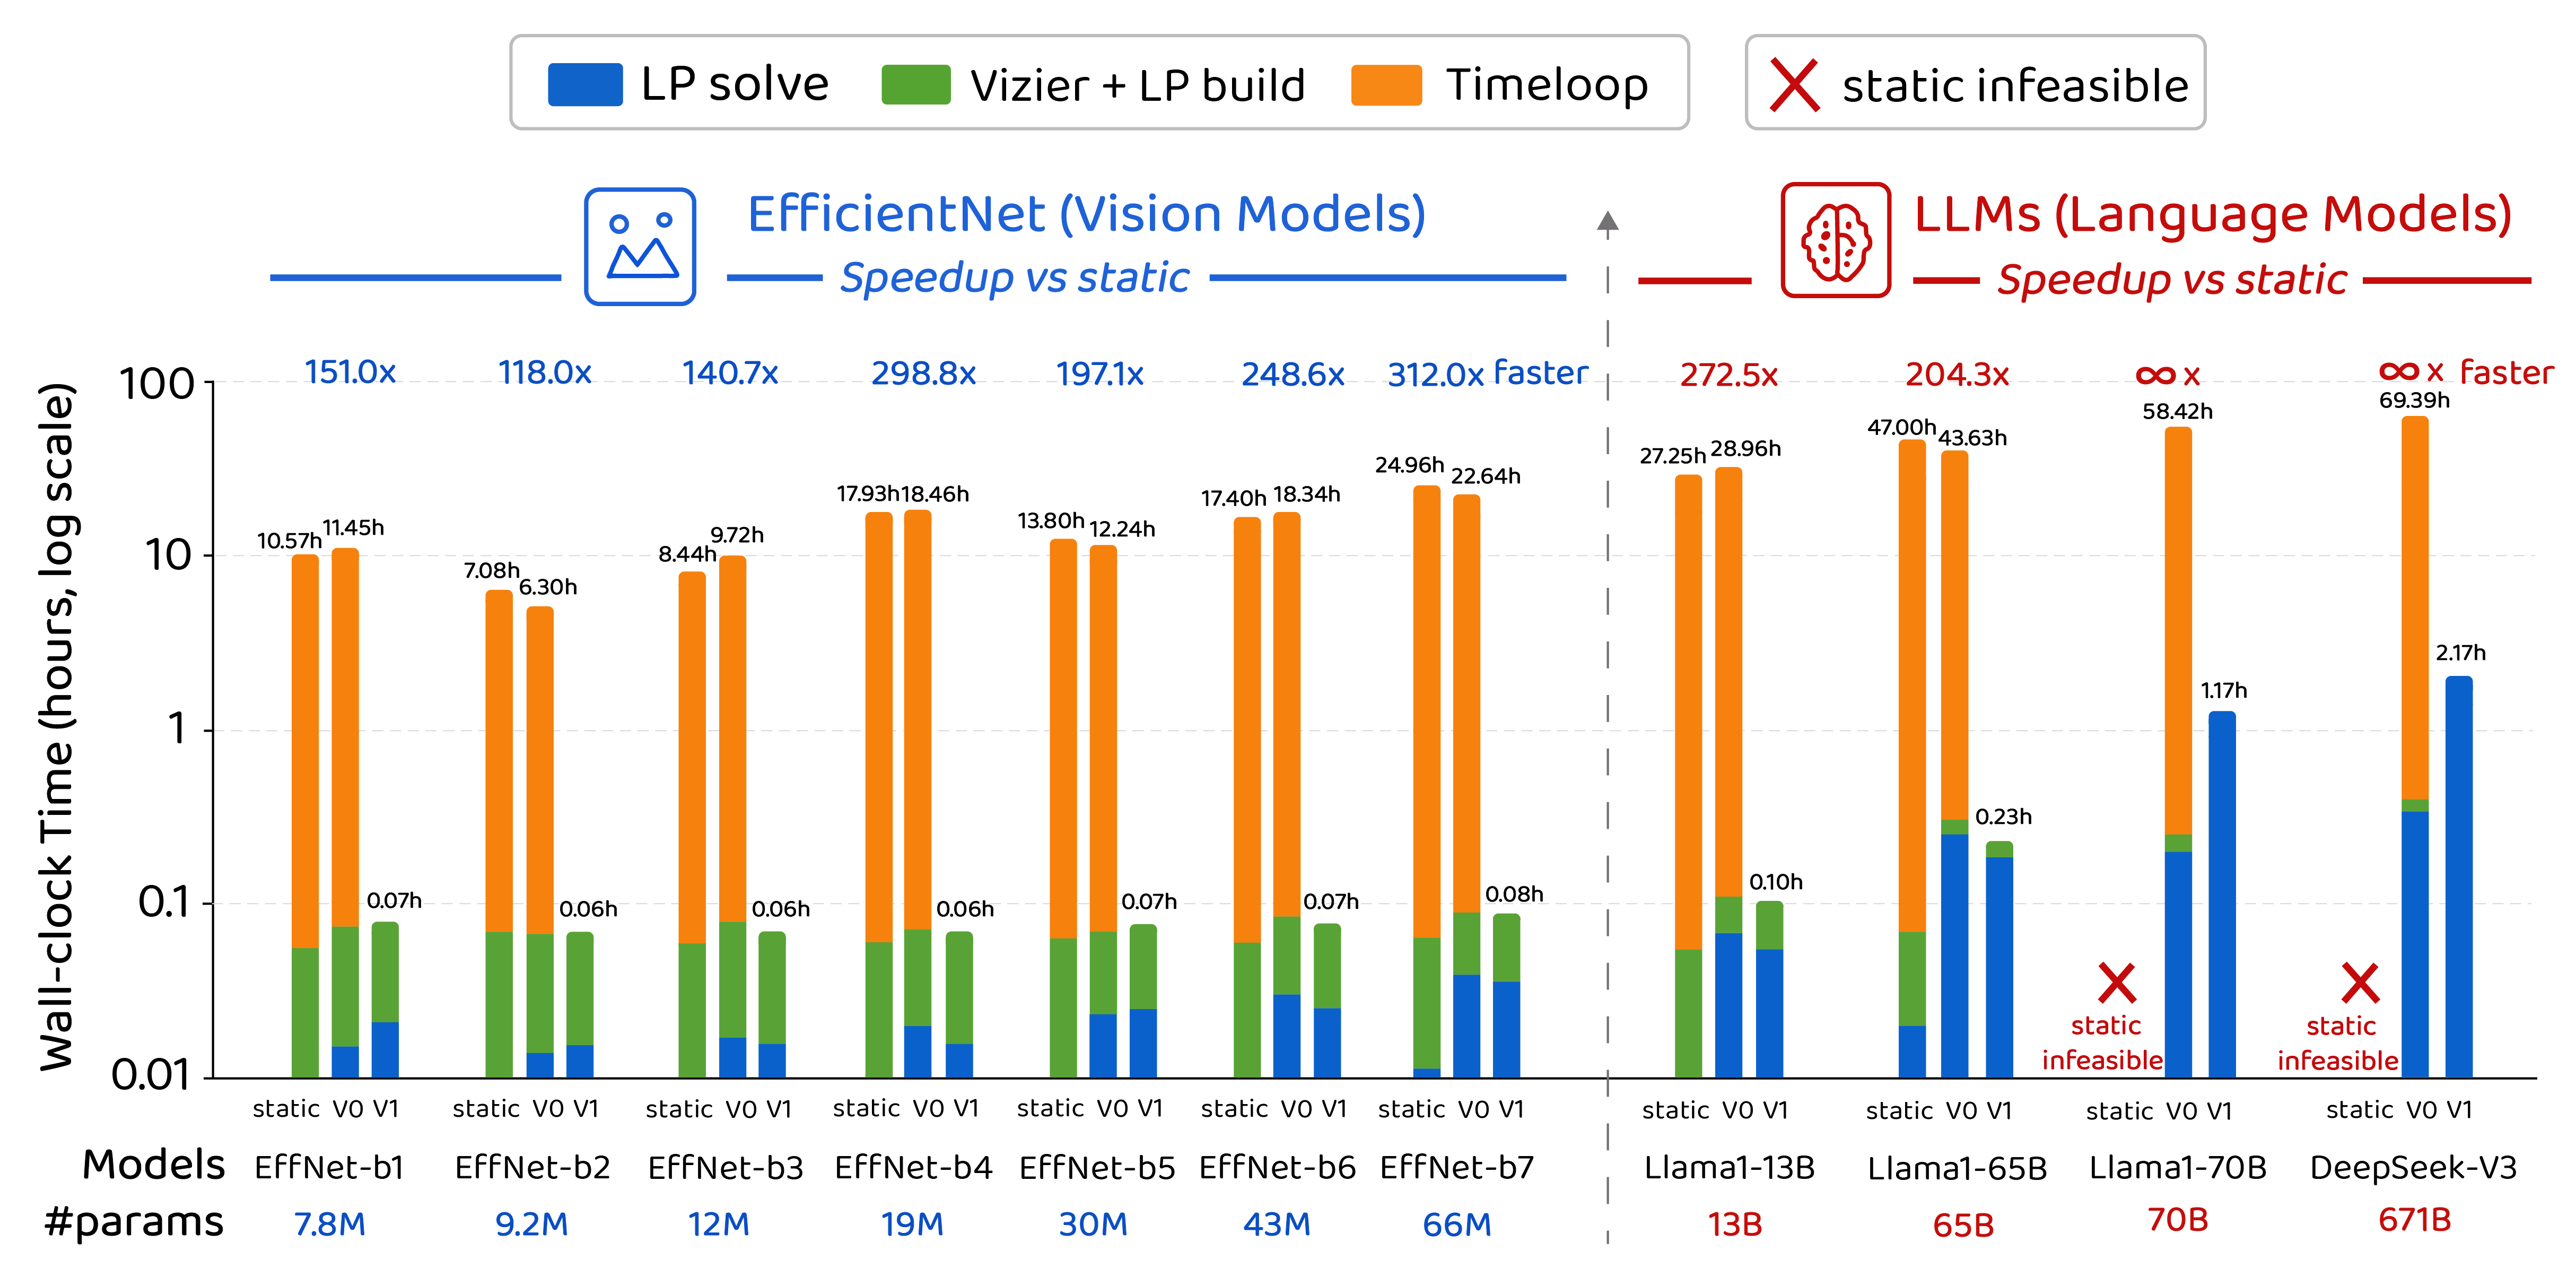
\includegraphics[width=1.0\linewidth]{fig3/wallclock_new_v5.png}
% % \caption{Wall-clock time decomposition and performance acceleration across formulations: CHEETAH-V1's internalized tiling eliminates the Timeloop bottleneck, achieving up to 100–300× faster search than classical static method.}
% % \label{fig:wallclock}
% % \end{figure}

% \begin{figure}[ht!]
%     \centering
% 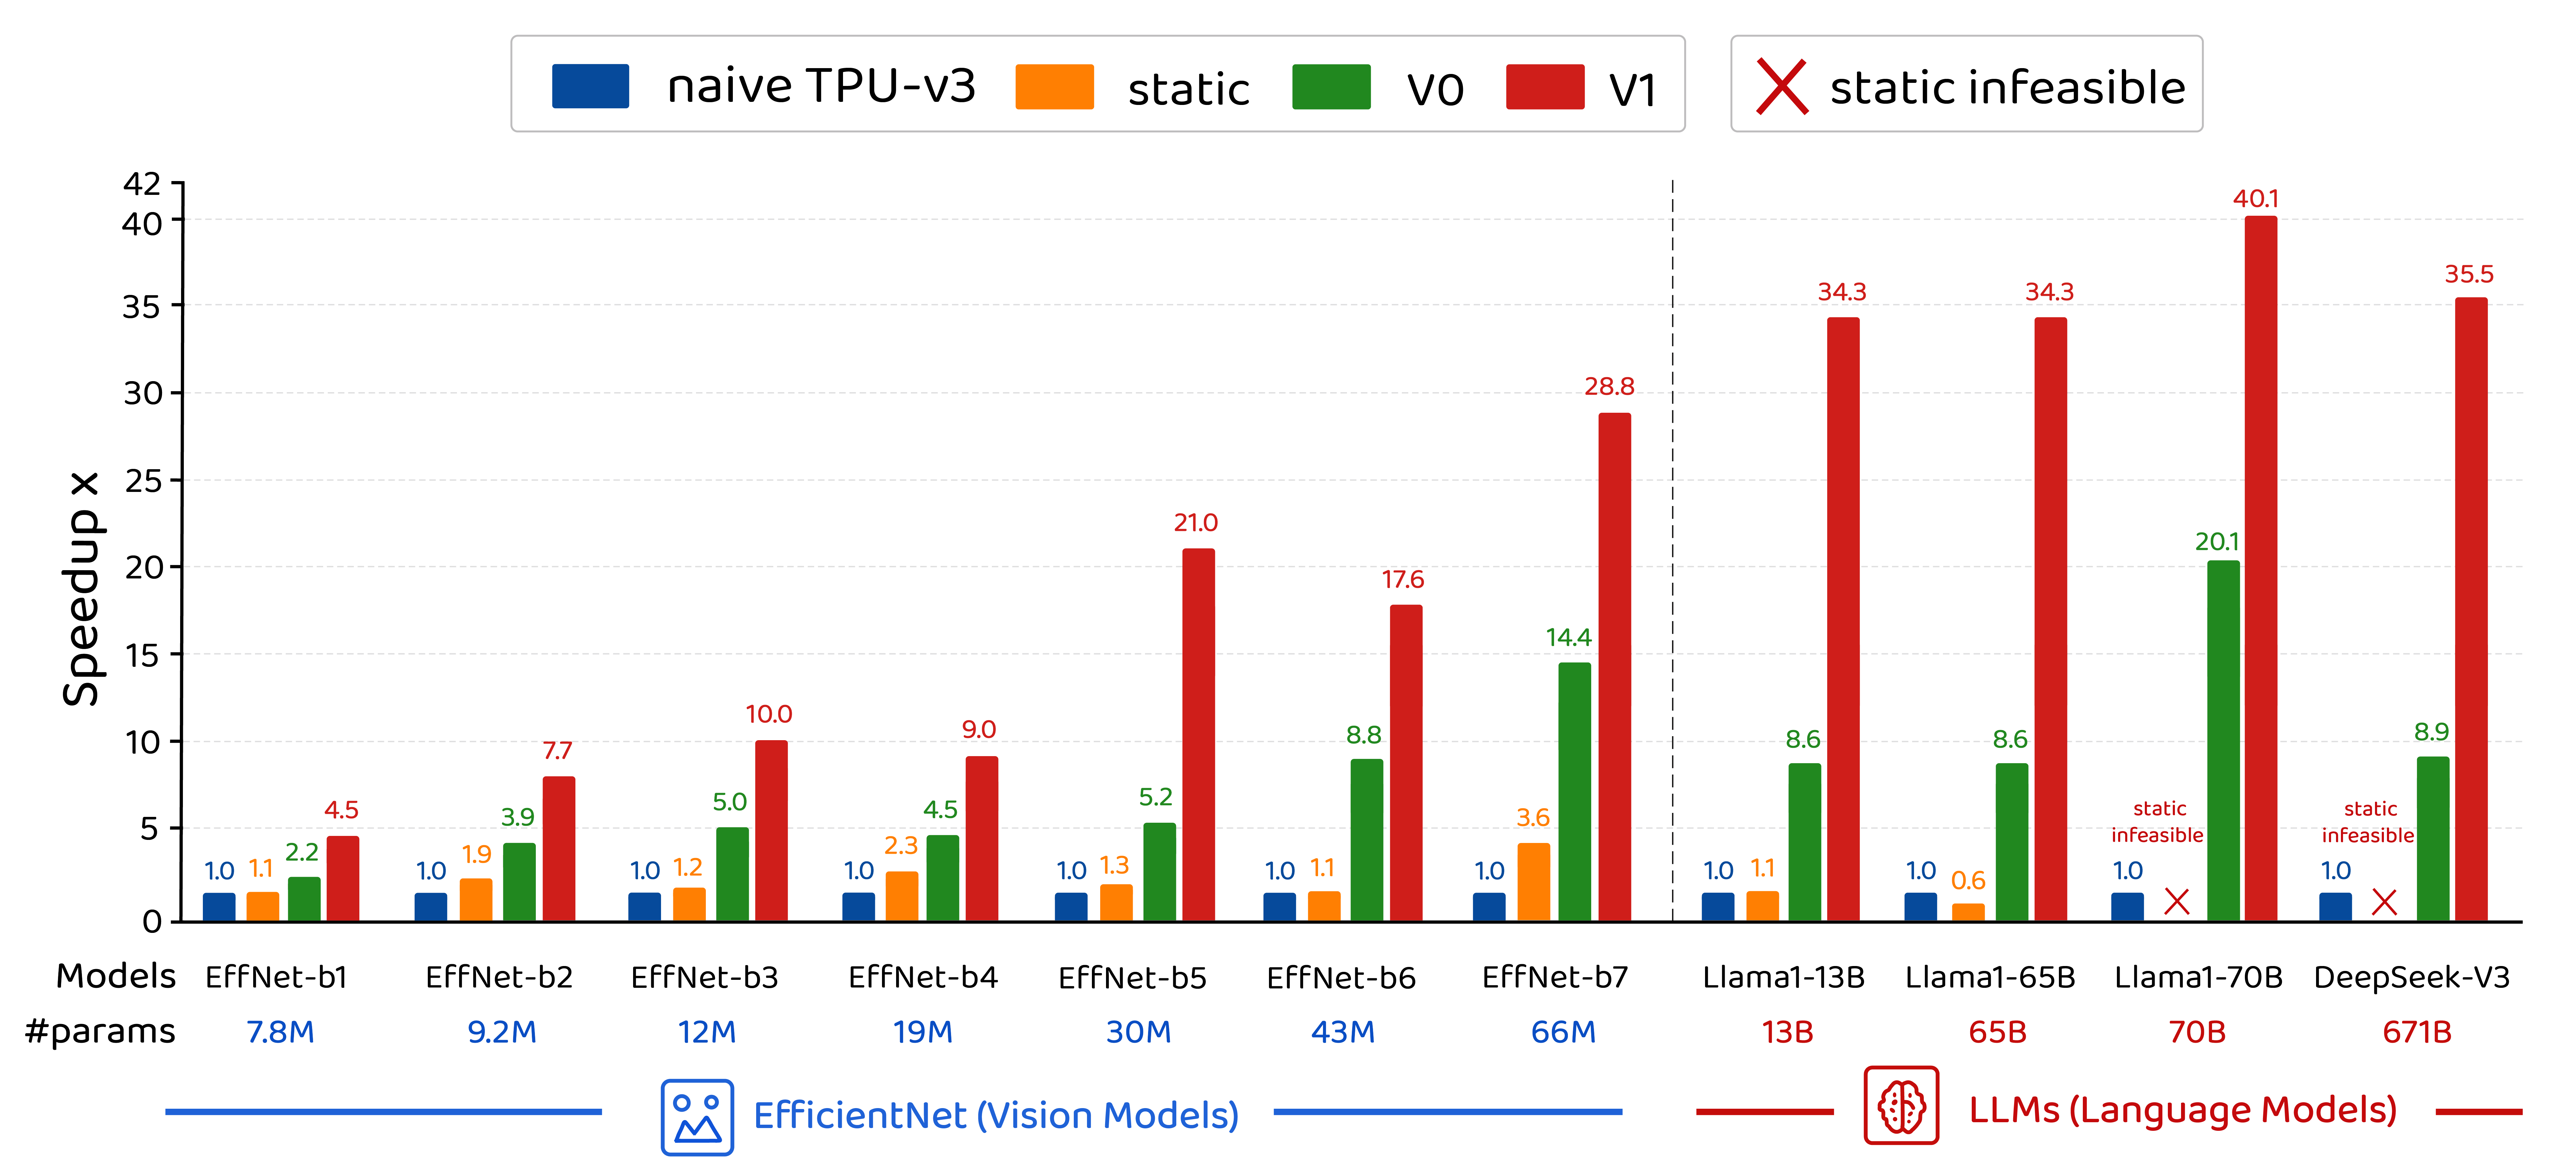
\includegraphics[width=1.0\linewidth]{fig3/speedup_final_v2.png}
% \caption{Speedup over modeled TPU-v3 baseline across formulations and workloads: CHEETAH-V1's joint tiling-fusion optimization achieves up to $\sim$35× acceleration, while static fusion is infeasible on large-scale LLMs.}
% \label{fig:speedup}
% \end{figure}

% % In addition to efficiently enabling more globally optimized accelerator designs, we anticipate that future work may build off this foundation to implement custom Flash Attention type speedup mechanisms for individual hardware (such as RTX5090) and workloads (such as LLama70B) tractably within hours, as well as quickly and efficiently design custom accelerators for targeted inference tasks. 
% % compromise on any single workload; a growing body of evidence suggests that workload-specialized designs can deliver $2$--$6\times$ improvements in performance per watt.
% % The resulting system replaces FAST's sequential Timeloop$\rightarrow$fusion~ILP pipeline with a single LP that jointly optimizes tiling, fusion, and memory scheduling, while preserving Vizier's outer loop over hardware configurations (or replacing it with LLM-guided search).

% % Furthermore, FAST's fusion ILP uses static tensor placement: a tensor is either pinned for the entire inference pass or not at all.
% % This is overly conservative for models with long dependency chains or skip connections, where different tensors are live at different times during execution.
% % A dynamic placement strategy that can evict and re-pin tensors across timesteps could substantially improve global memory utilization. Joint Optimization is the only way to solve the "Memory Wall" for large scale models like DeepSeek-V3.

% % FAST operates via a three-stage sequential pipeline (Figure \ref{fig::workflow}): (1)~a black-box optimizer (Google Vizier \citep{google_vizier}) proposes a hardware configuration defined by 16 hyperparameters---PE grid dimensions, systolic array sizes, buffer capacities, DRAM channels, and batch size; (2)~a scheduling engine (Timeloop \citep{timeloop}) finds the best tiling and mapping for each operation independently given the fixed hardware; and (3)~an integer linear program (ILP) decides which tensors to pin in the on-chip Global Memory to reduce DRAM traffic.
% % The result of each trial---predicted performance per TDP---is fed back to Vizier, which proposes the next hardware configuration, repeating for thousands of trials until convergence.


% % automate the framework with SkyDiscover Loop for profile and context aware co-design. Therefore in less than five hours, we are able to find an more performant design spec than the strongest baseline on designing , in terms of both perf/TDP and speedup. Our experiments also include freezing any hardware at input, and reducing the scheduling, tiling, etc search to just the LP can yield speedups of avg 2.2x than just the base hardware along. We anticipate that future work may build off this foundation to implement custom Flash Attention type speedup mechanisms for individual hardware (such as RTX5090) and workloads (such as LLama70B) tractably within hours. 

% % Our propose the formulation for global co-design for a custom accelerator as a large scale linear program which captures strict dependencies and tradeoffs sequential methods may miss. Our LP formulation captures scheduling, tiling, rematerialization, and is able to solve matrices at scales of $6{,}319 \times 4{,}516$,\ nnz$=829{,}852$ \& $3{,}669{,}793 \times 3{,}263{,}443$,\ nnz$=7{,}342{,}293$ \& $2{,}983{,}450 \times 2{,}504{,}019$,\ nnz$=6{,}094{,}156$ quickly, by utilizing a JAX based large scale solver. Our insight is that despite the challenging large scale of the problem, the structure of the matrices, once formed, retain the same structure. Therefore we are able to design one preconditioning scheme to these large scale systems matrices that can be re-used across any NN. This also allows us to capture dependencies prior methods cannot, for example our formulation introduces a dynamic placement strategy that can evict and re-pin tensors across timesteps could substantially improve global memory utilization. Joint Optimization is the only way to solve the "Memory Wall" for large scale models like DeepSeek-V3. 

% % For EfficientNet-B7 at $L=400$ operations and $T=400$ timesteps, the V1 LP contains approximately $2$ million variables and $5$ million constraints with $15$--$25$ million nonzeros. To better solve such large-scale LP problems more efficiently, we implement our own variant of a GPU-accelerated solver based on recent primal-dual LP algorithm \citep{applegate2022practicallargescalelinearprogramming}. We extend its original formulation in various ways and benchmark our implementation compared to existing commercial SciPy solvers, which showcase the advantage of our solver. To keep the main context clean and focused, we defer LP solver-related details to Appendix \ref{app:solver}.

% % A large number of black box optimization tools to handle this large search space have been recently proposed, such as Google's Vizier, Meta's AX, and Optuna. In addition search strategies are also explored, for example Google's Vizier proposes numerous methods Gaussian Process Upper Confidence Bound, Eagle Strategy as a metaheuristic optimization algorithm designed for global optimization via a two-stage hybrid approach that combines global exploration with intensive local search, and Linear Combination Swarm (LCS). However these methods share certain limitations, since they cannot globally capture the tradeoffs and tensions between sequential decisions and rely on brute force iterations. This requires human engineers to spend months of compute and thousands of repetitive trials to get improvements, without feedback on what might be globally optimal. 

% % While this sequential decomposition makes the problem tractable, it introduces a fundamental limitation: \emph{each stage takes the previous stage's output as fixed input, preventing the discovery of solutions that require trading off across stages.} Consider a concrete example: for a depthwise-separable convolution layer in a NN, a search tool such as Timeloop might select a tiling configuration that maximizes compute utilization at $74\%$, producing an activation working set of $6$ MiB. THe stacked The downstream fusion ILP solver tool receives this fixed working set size, cannot fit the tensor into the $128$ MiB Global Memory alongside other pinned tensors. However, an alternative tiling configuration with slightly lower utilization ($70\%$) might produce a working set of only $3$ MiB, enabling the fusion solver to pin an additional weight tensor that eliminates a DRAM bottleneck entirely, thus yielding a net $>20\%$ cycle reduction despite the $4\%$ utilization loss. Therefore these sequential pipelines systematically misses such cross-stage trade-offs.

% % The rapid evolution of deep learning workloads has created a compelling opportunity for domain-optimized inference accelerators.
% % Production models now serve billions of daily users, and the computational demands of architectures based on depthwise-separable convolutions (EfficientNet), self-attention (BERT, LLaMA), mixture-of-experts (DeepSeek-V3, Mixtral), and state-space models (Mamba) differ dramatically in their compute-to-memory ratios, tensor shapes, and data reuse patterns. However although the NN training strategy has been scaled up and we've done a lot of work on it, we now face the inference bottle neck era since general-purpose hardware, Nvidia's gaming GPUs are not necessarily optimized for deep learning tasks, and leaves a huge amount of compute on the table.


% page edit

\section{Introduction}
\label{sec:introduction}

\begin{figure}[ht!]
    \centering
    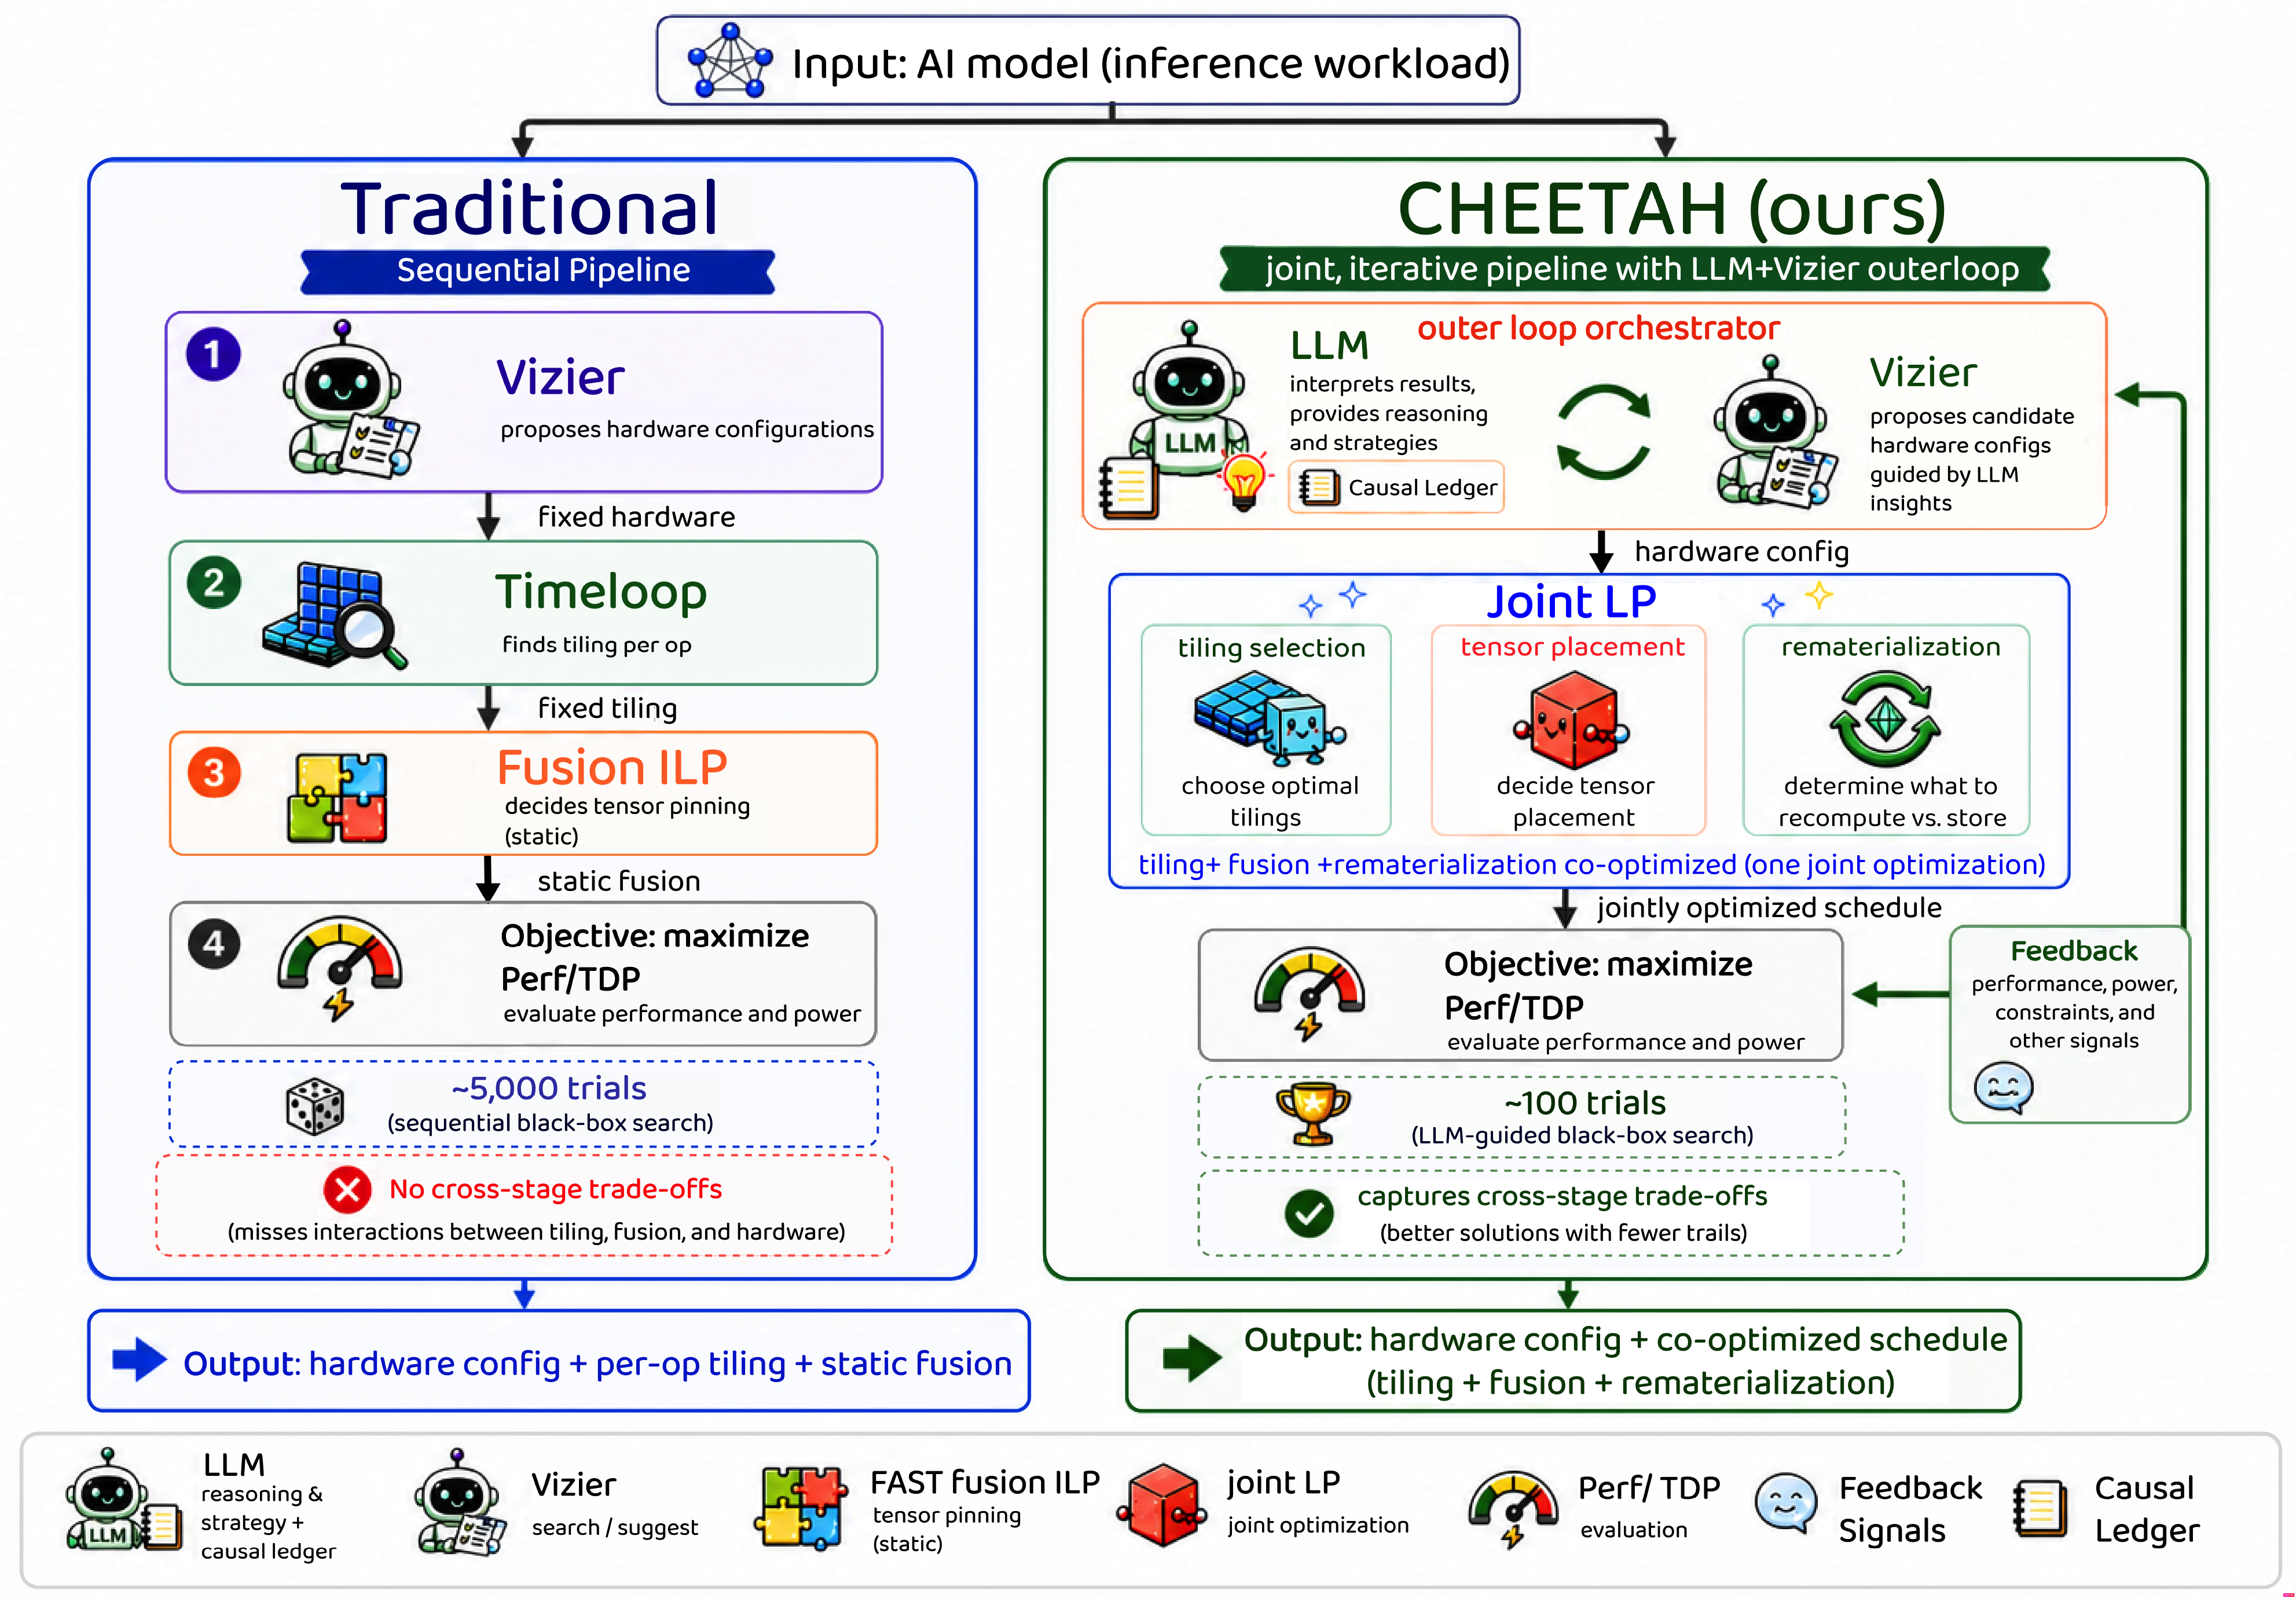
\includegraphics[width=1.0\linewidth]{figs/cheetah_v4_new.png}
    % \caption{\textbf{FAST vs.\ FAST-CORGI pipeline comparison.} 
\caption{Sequential vs Our Unified Optimization Paradigm.
(Left) Baseline methods decouple hardware search, operation-level tiling, and static fusion; precluding cross-stage trade-offs.
(Right) CHEETAH presents a unified LLM-driven LP-solver-based framework that jointly optimizes tiling, placement, and rematerialization while learning from a causal ledger.}
\label{fig::workflow}
\end{figure}
% The rapid evolution of deep learning workloads varies from convolutions to self-attention (LLaMA), mixture-of-experts (DeepSeek-V3), and state-space models (Mamba). These diverse architectures serve billions of daily users, and have fundamentally shifted the requirements for hardware acceleration. As foundation models continue to scale in parameters, the primary cost and bottleneck of model deployment has shifted from training to inference. Therefore much recent research has been focused on optimizing for more efficient execution and throughput across diverse, high-dimensional workloads. General-purpose GPUs remain largely designed for graphics-heavy throughput, and leave substantial efficiency and compute on the table at these tasks. Therefore we are motivated to design targeted accelerators that are optimized for handling the varying tensor shapes and data-reuse patterns of modern deep learning architectures.
% Much research has been done in accelerating inference through custom accelerator design, more efficient neural network (NN) batching algorithms, and domain specific packages and languages that aim to speed up general NN inference. For example, the widely adopted Flash Attention uses tiling to provide significant speedups by optimizing memory movement between SRAM and DRAM. Co-design takes this a step further by aiming to optimize hardware, software and scheduling to unlock performance neither could reach independently. The traditional framework of doing this is a sequential pipeline of heuristics tools, requiring human engineers to iterate through a large search space for months from testing for the size of DRAM, to determining higher level scheduling problems. Optimizing each piece of this complex pipeline is extremely challenging, since hardware datapaths, software schedules, and compiler transforms across a combinatorial space exceeding $\mathcal O(10^{2300})$.
The AI inference demand is expected to grow by $10,000\times$ over the next 5 years \citep{cra2026aifuture}. General-purpose accelerators leave significant efficiency gains unrealized, which motivates the design of targeted custom accelerators. Co-design, which jointly optimizes hardware-software (HW/SW), and scheduling for target workloads, offers a path to unlock performance efficiency for the upcoming inference era. However, the prevailing approach relies on sequential pipelines of heuristic tools, a slow, human-driven process navigating a combinatorial search space exceeding $\mathcal O(10^{2300})$ \citep{zhang_fast}. State-of-the-art frameworks like FAST \citep{zhang_fast} improve on this through an automated flow (a hardware proposer feeds an operation-level tiling agent, which feeds a downstream fusion solver), but remain fundamentally decoupled: a tiling that slightly reduces compute efficiency may shrink the working set enough to eliminate a DRAM bottleneck, yet sequential pipelines cannot discover such cross-stage trade-offs.

% The co-design problem is increasingly important as inference efficiency is the dominant AI workload and is rapidly growing. Therefore industry leaders such as NVIDIA and Google have designed chips for improved hardware-native agentic AI and , and state-of-the-art frameworks such as FAST, address this through a sequential decomposition of heuristics (a hardware proposer feeds an operation-level tiling agent, which feeds a downstream fusion solver). While FAST-generated accelerators can provide increased speedups over baseline TPU-v3, this decoupled approach is limited since it cannot capture cross-stage trade-offs. A tiling configuration that is \textit{locally} optimal for one layer may create an activation footprint that later prevents \textit{global} fusion, while a slightly slower tiling might shrink the working set enough to eliminate a DRAM bottleneck entirely. Sequential pipelines are systematically unable to express these interactions, leading to locally good but globally sub-optimal designs. 
Unifying the design space into a single convex relaxation yields previously infeasible global optima. Specifically, we introduce CHEETAH: a custom inference accelerator design framework that unlocks globally optimized designs with a dual-loop. Our inner-loop is a novel large-scale Linear Program (LP) to precisely mathematically model strict design decisions and constraints that must not be violated. The LP captures trade-offs for targeted workloads through time-indexed placement and rematerialization, thus allowing tensors to be dynamically pinned, evicted, recomputed across inference timesteps. We further extend our reformulation to internalize tiling selection into the LP, by introducing Pareto-pruned tiling variables and the McCormick linearization (a convex relaxation used for optimization of bilinear problems \citep{mccormick1976computability}). By exploiting the structural invariance of our matrices across hardware trials, we also adapt a GPU-accelerated primal-dual solver in JAX \citep{jax2018github} that can resolve millions of variables to rapidly reduce trial time from days to hours. This allows the LP solver to jointly reason about hardware configuration, activation placement, and weight pinning in a single pass, while providing feedback signal via Lagrangian duals.

\paragraph{One program, many architectures.} A natural question is how a single program can co-design accelerators for workloads as different as EfficientNet, the Llama family, DeepSeek-V3's mixture-of-experts, and the Stable Diffusion UNet. The LP is \emph{not} per-architecture: it is defined over a generic graph intermediate representation, a directed acyclic graph of operations, each carrying a Timeloop-derived tile-configuration Pareto set and a roofline, connected by edges with residency. A depthwise convolution, a dense GEMM, an attention matmul, and an expert feed-forward are all simply ``operations with shapes''; the architecture-specific content lives entirely in the coefficients (operation shapes, Pareto data, and edge topology), never in the structure of the program. Architecture-specific decisions (a KV-cache budget, mixture-of-experts expert-residency, diffusion cross-step reuse) are optional constraint families that switch on only when the relevant operation type is present and are inert otherwise. One program therefore covers every architecture the way a single register allocator compiles every source language: it operates on the graph, not the workload.

Our outer-loop framework stacks a black-box optimizer (Google Vizier \citep{google_vizier}) to propose candidate hardware configurations defined by a set of hyperparameters (e.g., processing element grid dimensions, systolic array sizes, DRAM size, etc), while a LLM is used for efficient search-space steering. The LLM acts as a causal architect, interpreting a compact trial ledger of roofline checks and LP feedback diagnostics to propose constrained architectural search input for Vizier. This prevents the search-space gaming typical of black-box optimizers in wide design regions, and reduces the need for thousands of sequential trials via Bayesian search strategies in Vizier to learn good vs bad neighborhoods in search topology. Our results demonstrate that the LLM Architect framework further reduces invalid hardware trials from 24.5\% under vanilla Vizier to 5.9\%, to reach the Pareto frontier faster than the next strongest baseline. We validate all results with Model Flop Utilization (MFU) and roofline lower-bound audits, ensuring predicted latencies are physically grounded in compute and memory throughput limits. Figure~\ref{fig::workflow} outlines the comparative difference between the standard sequential workflow and our joint optimization paradigm. 
% \todo{Add best of both worlds, strengths from principled LP side, from LLM aggregate info side}
% \todo{Aggregates past experience to gain insight into steering hardware-software co-design. We offload the strict solves, with constraints that must the strictly respected, to the LP solve part. This combines the best of both worlds.} 
\paragraph{Contributions.} We reformulate the fundamental HW/SW co-design problem into a unified  framework in CHEETAH, combining principled mathematical rigor of the LP formulation to solve strict design decisions optimally, with the powerful aggregation and causal learning of an LLM Architect outer loop for meta-optimization. Our open-source repository for full reproducibility is at \href{https://anonymous.4open.science/r/CHEETAH-B268/readme}{https://anonymous.4open.science/r/CHEETAH-B268/}.

\begin{enumerate}
    \item \textbf{CHEETAH-V0 - Dynamic Placement with Rematerialization:}
    We introduce time-indexed LP variables $p_{i,t}^k$ and rematerialization variables $r_{i,t}$ to enable cheap recompute operations instead of paying DRAM reload costs, supporting skip connections and multi-fanout nodes.

    \item \textbf{CHEETAH-V1 and V3 - Joint Tiling-Fusion via Classical Convex Modeling:}
    We unify tiling and fusion into a single LP problem by introducing tiling selection variables $y_{i,c}$, and employ \textbf{McCormick envelopes} to exactly linearize the bilinear interaction between tiling and tensor pinning; V3 then promotes the chip's MAC count and bandwidth to decisions and replaces the aggregate roofline with a \textbf{disaggregated perspective epigraph} that is the exact convex hull of the per-tile roofline disjunction. Both are classical tools of mathematical programming (McCormick's 1976 envelopes and epigraph/perspective reformulation) that the accelerator co-design literature does not use, because its pipelines are built from simulators and heuristics rather than from programs. Applied here they buy two things at once: a parameter-free relaxation that is exact at every integer vertex, so the LP is simultaneously an optimizer and a valid lower bound, and a coupling that internalizes the tiling-placement trade-off to discover design points that sequential pipelines systematically miss.
    % This enables the LP to discover trade-offs where accepting a suboptimal tiling configuration enables superior fusion, or vice versa---precisely the cross-stage interactions that the sequential pipeline cannot capture.
    \item \textbf{VM-One-Armed-Rescue Solver:} The McCormick linearization that makes V1 exact also \emph{blows up} the constraint matrix (for DeepSeek-V3, ${\sim}2.5$M variables, ${\sim}3.0$M constraints, and ${\sim}6.1$M nonzeros) and leaves it severely ill-conditioned, with coefficients spanning ${\sim}10$ orders of magnitude. Stock first-order GPU solvers (cuPDLP) and CPU simplex/barrier (HiGHS) stall or diverge, with the primal or dual side lagging. We introduce \textbf{VM-One-Armed-Rescue}, a matrix-free JAX solver that augments restarted PDHG with a diagonal \emph{variable-metric} rescaling and a one-sided ``rescue'' restart, resolving these LPs to dual convergence in seconds. To our knowledge it is the first solver to make the McCormick-linearized joint tiling--fusion--placement co-design LP tractable at LLM scale: the enabling step that collapses a days-long search into hours (Section~\ref{sec:solver_vm}).

    \item \textbf{LLM-guided Causal Architect:} The LLM outer loop steers hardware search by interpreting \emph{converged Lagrangian dual signals} from the inner LP together with a Causal Ledger of past trials to perform targeted subspace interventions, transforming black-box search into a structured, diagnostic-driven process. To our knowledge, CHEETAH is the \textbf{first} to steer an LLM-guided architecture search with the converged Lagrangian dual variables of a co-design LP: the duals \emph{indicate} where to search while the LP retains every optimality certificate; the LLM proposes, the solver never loses rigor. The Architect guides Vizier through widened search spaces, reducing invalid trials by ${\sim}4\times$ ($24.5\%\!\to\!5.9\%$) while preserving the global optimal score, and enables profile-specific designs (speech models may emphasize latency, while data-synthesis models may prioritize bandwidth).
    \item \textbf{Certificates, not counters:} Every CHEETAH schedule ships with an LP optimality certificate: the converged dual bound against which the realized schedule is measured, with the relaxation gap reported per workload and the integral optimum certified exactly on chain-structured models. A cycle-accurate RTL replay then confirms, decision by decision (tile choice, residency, eviction, rematerialization), that the plan executed as planned with byte-exact memory occupancy. This is a stronger guarantee than the ``did the optimization fire'' checks that agentic kernel optimizers use to validate hardware-aware code~\citep{tschand2026hawkeye}: a counter confirms a feature was used, a certificate bounds how far the result can be from optimal.

    \item \textbf{Speedup:} Our method demonstrates an average speedup of $\sim22.07\times$ over the baseline across a wide range of $12$ workloads ($11$ vision and language models plus the Stable Diffusion~1.5 UNet), reaching up to ${\sim}40.1\times$ on a single workload, as shown in Figure~\ref{fig:speedup} below. \todo{averages and Figure~\ref{fig:speedup} to be refreshed once SD1.5-UNet is added to the search plots}

    % profiles into consideration to push the black-box optimizer responsible for hardware suggestions to output with structured reasoning about architectural trade-offs. 

\end{enumerate}

\begin{figure}[ht!]
    \centering
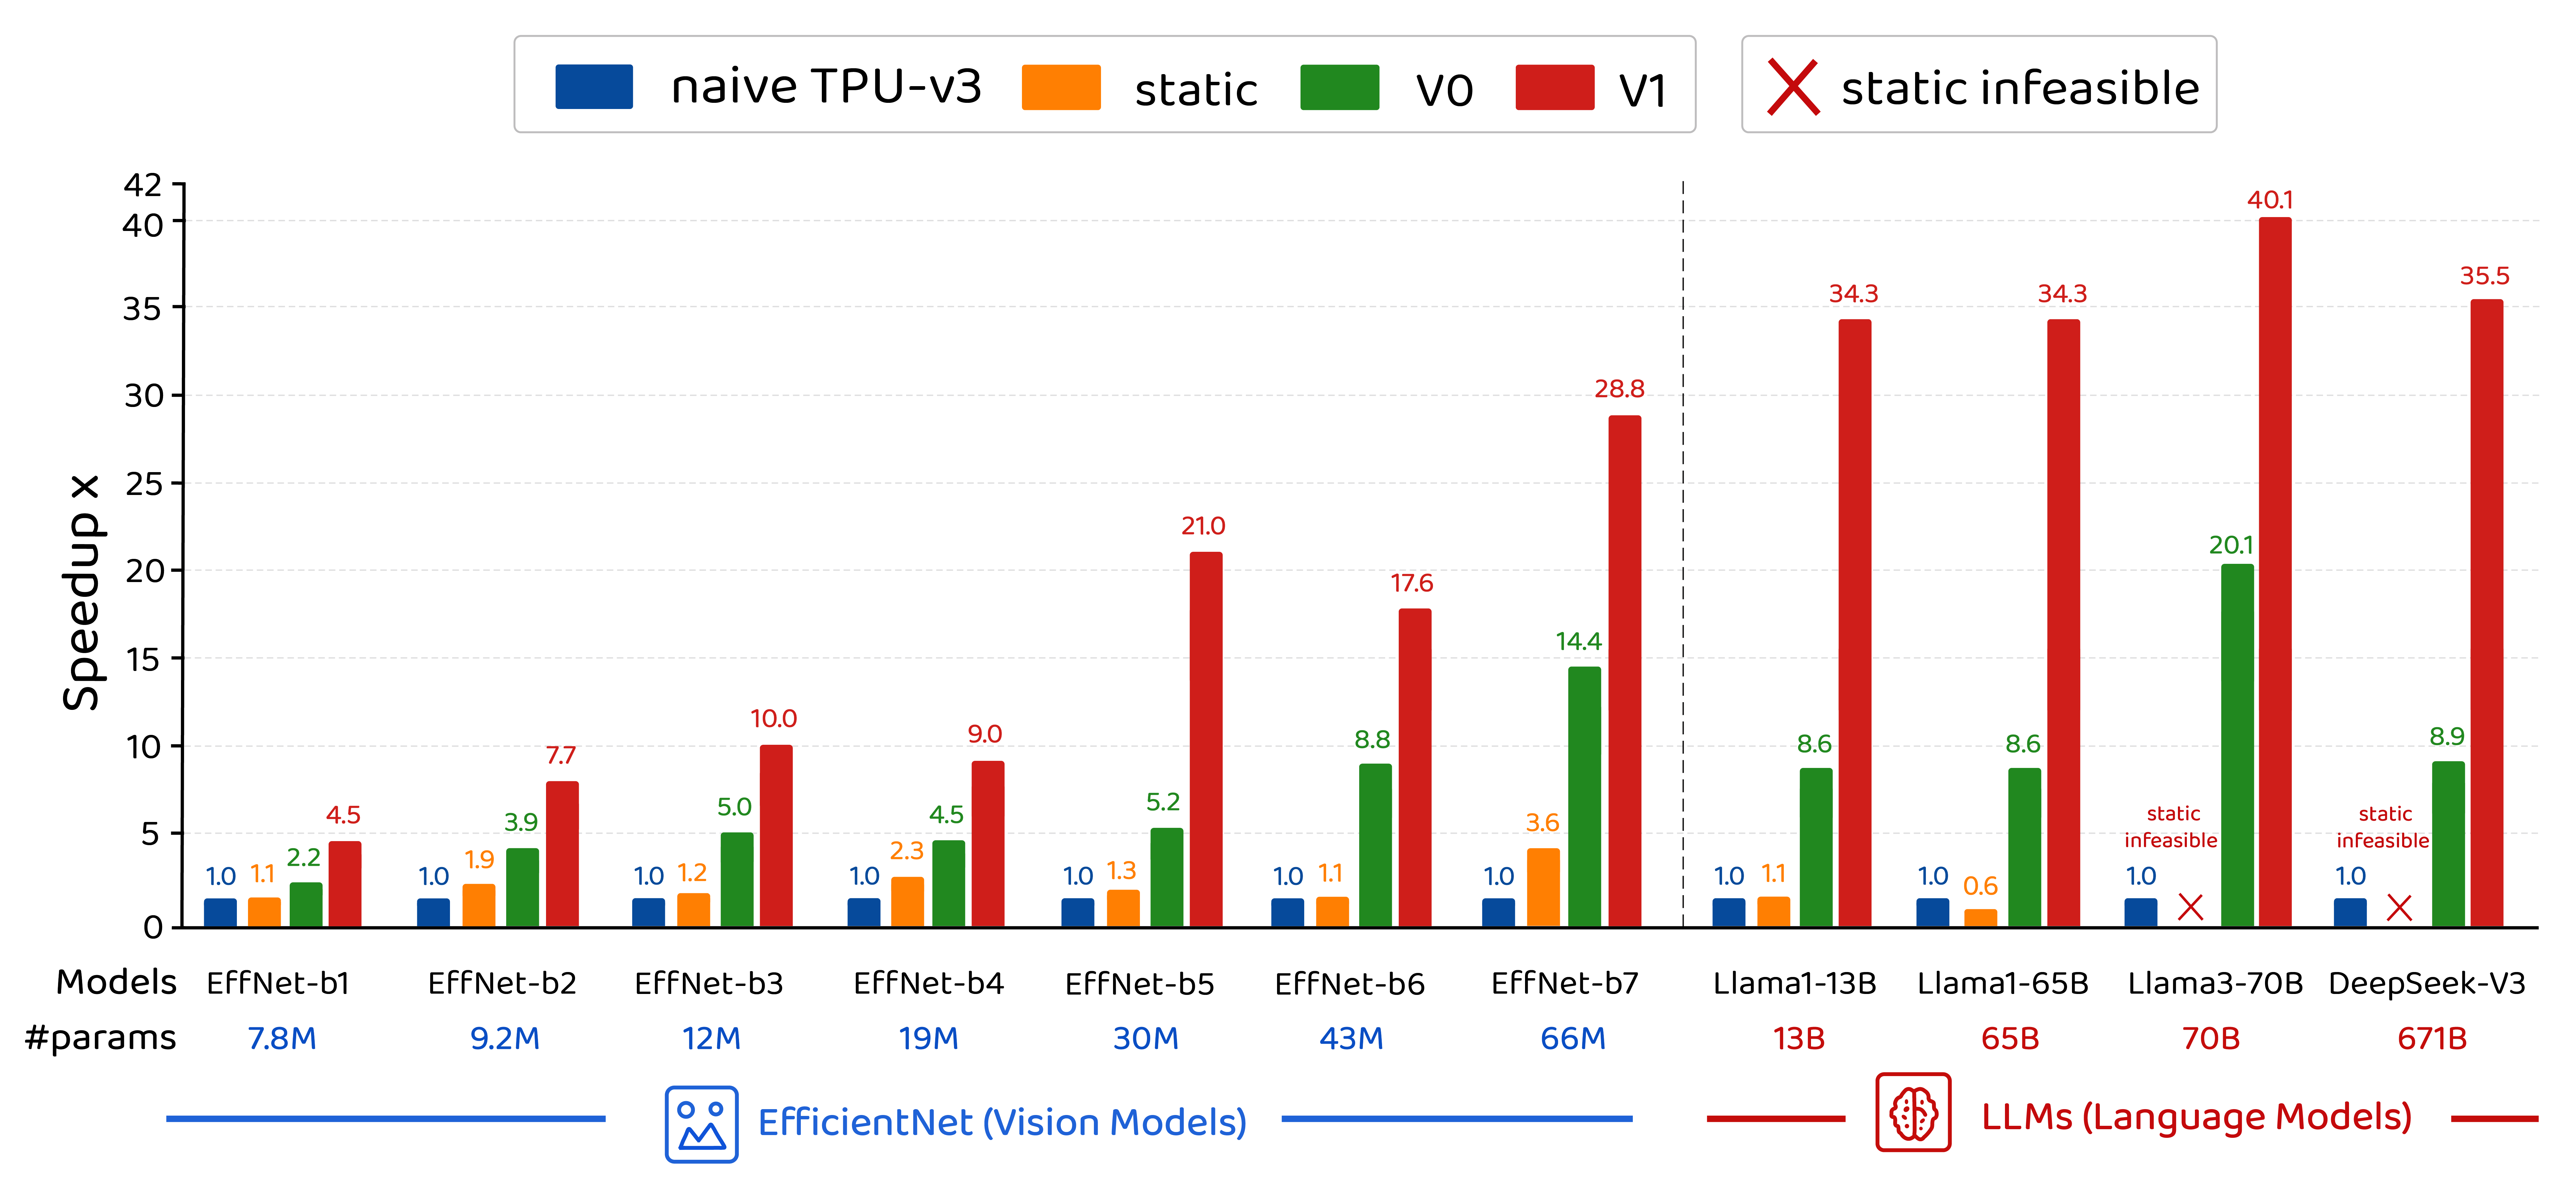
\includegraphics[width=1.0\linewidth]{fig3/speedup_final_v3.png}
\caption{Speedup over modeled TPU-v3 baseline for each workload and formulation: CHEETAH-V1's joint tiling-fusion optimization achieves up to $\sim$40.1$\times$ acceleration, while static fusion is infeasible on large-scale LLMs. Progressive gains are visible across formulations: V0's dynamic placement improves over static by $2$--$20\times$, while V1's joint tiling-fusion adds another $2$--$4\times$ on top. See Section~\ref{sec:experiments} for full analysis and wall-clock time breakdowns.}
\label{fig:speedup}
\end{figure}

CHEETAH reframes accelerator co-design from a sequential pipeline of heuristics into a single certified optimization. Its inner LP provably \emph{contains} the map-then-fuse pipelines of prior work (Theorem~\ref{thm:containment}) and returns a certified lower bound on schedule quality, so the field's usual ``$N\times$ over a baseline'' becomes ``within a certified gap of the optimum''; its outer loop couples this rigor with an LLM that reads the LP's own Lagrangian duals to steer the hardware search. The consequences are concrete: a ${\sim}22\times$ average (up to ${\sim}40\times$) speedup over a modeled TPU-v3 across $12$ vision, language, and diffusion workloads, every design validated by cycle-accurate RTL, six physical-feasibility gates, and roofline lower-bound audits, and a co-design loop that runs in \emph{hours} rather than months. The human's role shifts accordingly: they write constraints (area, power, capacity, and the cost model), not designs, and a new chip or a new workload enters the same program as new columns and rows rather than as a new search. We view this as a step-change in \emph{how} accelerators are designed: not a faster point inside an existing search, but a reformulation that makes the global optimum (and a proof of how close a design sits to it) attainable for the inference era.

\paragraph{Beyond prefill: shrinking the decode memory wall.} The speedups above are largest in the compute-bound \emph{prefill} phase, where scheduling has the most room. Realistic LLM \emph{serving}, however, is dominated by autoregressive \emph{decode}, where generating each token reloads the full weights and a growing KV cache from DRAM: the bottleneck shifts from compute to memory, and on fixed hardware no schedule can move it because the bytes are schedule-invariant. CHEETAH's co-design attacks this wall directly and jointly, by \emph{sizing on-chip global memory against a bounded, quantized KV cache} so that the cache is co-designed to fit on chip and its per-token read never touches DRAM. \todo{STALE FRAMING: our own newer results (\cref{sec:batch_sensitivity}, App.~N, Limitations) show the decode wall is MoE WEIGHT RELOAD (${\sim}98\%$ of decode traffic) with KV negligible. Rewrite this and the matching abstract clause around the sparse-routing/speculation story already written below.}The structural insight the program exploits is that on-chip memory should hold the KV cache, not the weights: model weights ($13$--$70$\,GB) cannot fit and must stream, but the KV cache can be bounded by eviction and shrunk by quantization until it fits, and it is re-read every decode step, so every byte of on-chip memory spent on it pays off once per generated token. Sizing the global buffer, the eviction budget, and the KV precision in one program is what shrinks the decode memory wall.

\paragraph{Why the decode wall does not dissolve under load: sparse routing defeats batching.}
For a dense model the decode memory wall is, in principle, a low-batch problem:
a larger serving batch amortizes each weight load perfectly, because the same
weights serve every token in the batch, so at high enough throughput the wall
recedes on its own. A sparse mixture of experts breaks this argument, and this
is what makes the co-design necessary rather than merely convenient. Under
top-$k$ routing the set of experts a decode step must load is the \emph{union}
of the experts its tokens select, so a larger batch touches \emph{more} experts:
the expected number of distinct experts follows $n(1-(1-k/n)^{B})$, which for
DeepSeek-V3 ($n=256$, $k=8$) rises from $8$ experts at $B=1$ to $163$ at
$B=32$ and $252$ at $B=128$. The reload therefore \emph{grows} with batch,
from $19$ to $598$~GB per step across that range, and although the per-token
cost does fall, it falls only from $19$ to $4.7$~GB, a $4\times$ amortization
bought with a $128\times$ increase in batch, and it saturates once essentially
every expert is swept. The wall is thus a structural property of sparse serving
rather than an artifact of small batches, and we confirm the consequence
empirically in \cref{sec:batch_sensitivity}: the speculative width the program
selects rises rather than collapses as batch grows, doubling with every
fourfold increase in batch, and the certified serving advantage rises
monotonically from $33.1\times$ at $B=1$ to $48.6\times$ at $B=128$. Two
mechanisms that are usually described as competing amortizers, batching and
speculation, are complementary here, precisely because batching amortizes so
poorly under sparse routing.

We present the work as a progression, so that each formulation's contribution can be read on its own terms. Section~\ref{sec:related} positions CHEETAH against prior mapping, co-design, and compilation systems (Table~\ref{tab:capability-matrix}). Section~\ref{sec:methods} builds the formulation in rungs: CHEETAH-V0 (Section~\ref{sec:v0}) adds time-indexed placement and rematerialization to the static fusion ILP; V1 (Section~\ref{sec:v1}) brings tiling inside the program, using Pareto pruning to compress the raw tile space and McCormick envelopes to flatten the resulting bilinear coupling into a linear program; V2 adds memory sizing and tile-dependent residency; and V3 (Section~\ref{sec:v1}) promotes the hardware itself to a decision under a disaggregated perspective epigraph, with the solver (Section~\ref{sec:solver_vm}) and the LLM-guided outer loop closing the loop. Section~\ref{sec:experiments} reports the progressive gains across these rungs together with the same-silicon fixed-hardware study, each result grounded by roofline, MFU, and manufacturability validators; Section~\ref{sec:rtl_validation} replays the schedules on cycle-accurate RTL; Section~\ref{sec:tco} reads the outcome in FAST's own cost model; and the appendices carry the containment theory, the solver, and the deficit and sensitivity analyses.

% In addition to efficiently enabling more globally optimized accelerator designs, we anticipate that future work may build off this foundation to implement custom Flash Attention type speedup mechanisms for individual hardware (such as RTX5090) and workloads (such as LLama70B) tractably within hours, as well as quickly and efficiently design custom accelerators for targeted inference tasks. 
% compromise on any single workload; a growing body of evidence suggests that workload-specialized designs can deliver $2$--$6\times$ improvements in performance per watt.
% The resulting system replaces FAST's sequential Timeloop$\rightarrow$fusion~ILP pipeline with a single LP that jointly optimizes tiling, fusion, and memory scheduling, while preserving Vizier's outer loop over hardware configurations (or replacing it with LLM-guided search).

% Furthermore, FAST's fusion ILP uses static tensor placement: a tensor is either pinned for the entire inference pass or not at all.
% This is overly conservative for models with long dependency chains or skip connections, where different tensors are live at different times during execution.
% A dynamic placement strategy that can evict and re-pin tensors across timesteps could substantially improve global memory utilization. Joint Optimization is the only way to solve the "Memory Wall" for large scale models like DeepSeek-V3.

% FAST operates via a three-stage sequential pipeline (Figure \ref{fig::workflow}): (1)~a black-box optimizer (Google Vizier \citep{google_vizier}) proposes a hardware configuration defined by 16 hyperparameters---PE grid dimensions, systolic array sizes, buffer capacities, DRAM channels, and batch size; (2)~a scheduling engine (Timeloop \citep{timeloop}) finds the best tiling and mapping for each operation independently given the fixed hardware; and (3)~an integer linear program (ILP) decides which tensors to pin in the on-chip Global Memory to reduce DRAM traffic.
% The result of each trial---predicted performance per TDP---is fed back to Vizier, which proposes the next hardware configuration, repeating for thousands of trials until convergence.


% automate the framework with SkyDiscover Loop for profile and context aware co-design. Therefore in less than five hours, we are able to find an more performant design spec than the strongest baseline on designing , in terms of both perf/TDP and speedup. Our experiments also include freezing any hardware at input, and reducing the scheduling, tiling, etc search to just the LP can yield speedups of avg 2.2x than just the base hardware along. We anticipate that future work may build off this foundation to implement custom Flash Attention type speedup mechanisms for individual hardware (such as RTX5090) and workloads (such as LLama70B) tractably within hours. 

% Our propose the formulation for global co-design for a custom accelerator as a large scale linear program which captures strict dependencies and tradeoffs sequential methods may miss. Our LP formulation captures scheduling, tiling, rematerialization, and is able to solve matrices at scales of $6{,}319 \times 4{,}516$,\ nnz$=829{,}852$ \& $3{,}669{,}793 \times 3{,}263{,}443$,\ nnz$=7{,}342{,}293$ \& $2{,}983{,}450 \times 2{,}504{,}019$,\ nnz$=6{,}094{,}156$ quickly, by utilizing a JAX based large scale solver. Our insight is that despite the challenging large scale of the problem, the structure of the matrices, once formed, retain the same structure. Therefore we are able to design one preconditioning scheme to these large scale systems matrices that can be re-used across any NN. This also allows us to capture dependencies prior methods cannot, for example our formulation introduces a dynamic placement strategy that can evict and re-pin tensors across timesteps could substantially improve global memory utilization. Joint Optimization is the only way to solve the "Memory Wall" for large scale models like DeepSeek-V3. 

% For EfficientNet-B7 at $L=400$ operations and $T=400$ timesteps, the V1 LP contains approximately $2$ million variables and $5$ million constraints with $15$--$25$ million nonzeros. To better solve such large-scale LP problems more efficiently, we implement our own variant of a GPU-accelerated solver based on recent primal-dual LP algorithm \citep{applegate2022practicallargescalelinearprogramming}. We extend its original formulation in various ways and benchmark our implementation compared to existing commercial SciPy solvers, which showcase the advantage of our solver. To keep the main context clean and focused, we defer LP solver-related details to Appendix \ref{app:solver}.

% A large number of black box optimization tools to handle this large search space have been recently proposed, such as Google's Vizier, Meta's AX, and Optuna. In addition search strategies are also explored, for example Google's Vizier proposes numerous methods Gaussian Process Upper Confidence Bound, Eagle Strategy as a metaheuristic optimization algorithm designed for global optimization via a two-stage hybrid approach that combines global exploration with intensive local search, and Linear Combination Swarm (LCS). However these methods share certain limitations, since they cannot globally capture the tradeoffs and tensions between sequential decisions and rely on brute force iterations. This requires human engineers to spend months of compute and thousands of repetitive trials to get improvements, without feedback on what might be globally optimal. 

% While this sequential decomposition makes the problem tractable, it introduces a fundamental limitation: \emph{each stage takes the previous stage's output as fixed input, preventing the discovery of solutions that require trading off across stages.} Consider a concrete example: for a depthwise-separable convolution layer in a NN, a search tool such as Timeloop might select a tiling configuration that maximizes compute utilization at $74\%$, producing an activation working set of $6$ MiB. THe stacked The downstream fusion ILP solver tool receives this fixed working set size, cannot fit the tensor into the $128$ MiB Global Memory alongside other pinned tensors. However, an alternative tiling configuration with slightly lower utilization ($70\%$) might produce a working set of only $3$ MiB, enabling the fusion solver to pin an additional weight tensor that eliminates a DRAM bottleneck entirely, thus yielding a net $>20\%$ cycle reduction despite the $4\%$ utilization loss. Therefore these sequential pipelines systematically misses such cross-stage trade-offs.

% The rapid evolution of deep learning workloads has created a compelling opportunity for domain-optimized inference accelerators.
% Production models now serve billions of daily users, and the computational demands of architectures based on depthwise-separable convolutions (EfficientNet), self-attention (BERT, LLaMA), mixture-of-experts (DeepSeek-V3, Mixtral), and state-space models (Mamba) differ dramatically in their compute-to-memory ratios, tensor shapes, and data reuse patterns. However although the NN training strategy has been scaled up and we've done a lot of work on it, we now face the inference bottle neck era since general-purpose hardware, Nvidia's gaming GPUs are not necessarily optimized for deep learning tasks, and leaves a huge amount of compute on the table.
% \section{Related Work}
% \label{sec:related}

% % \subsection{FAST: Full-stack Accelerator Search Technique}
% % \begin{figure}[ht!]
% %     \centering
% %     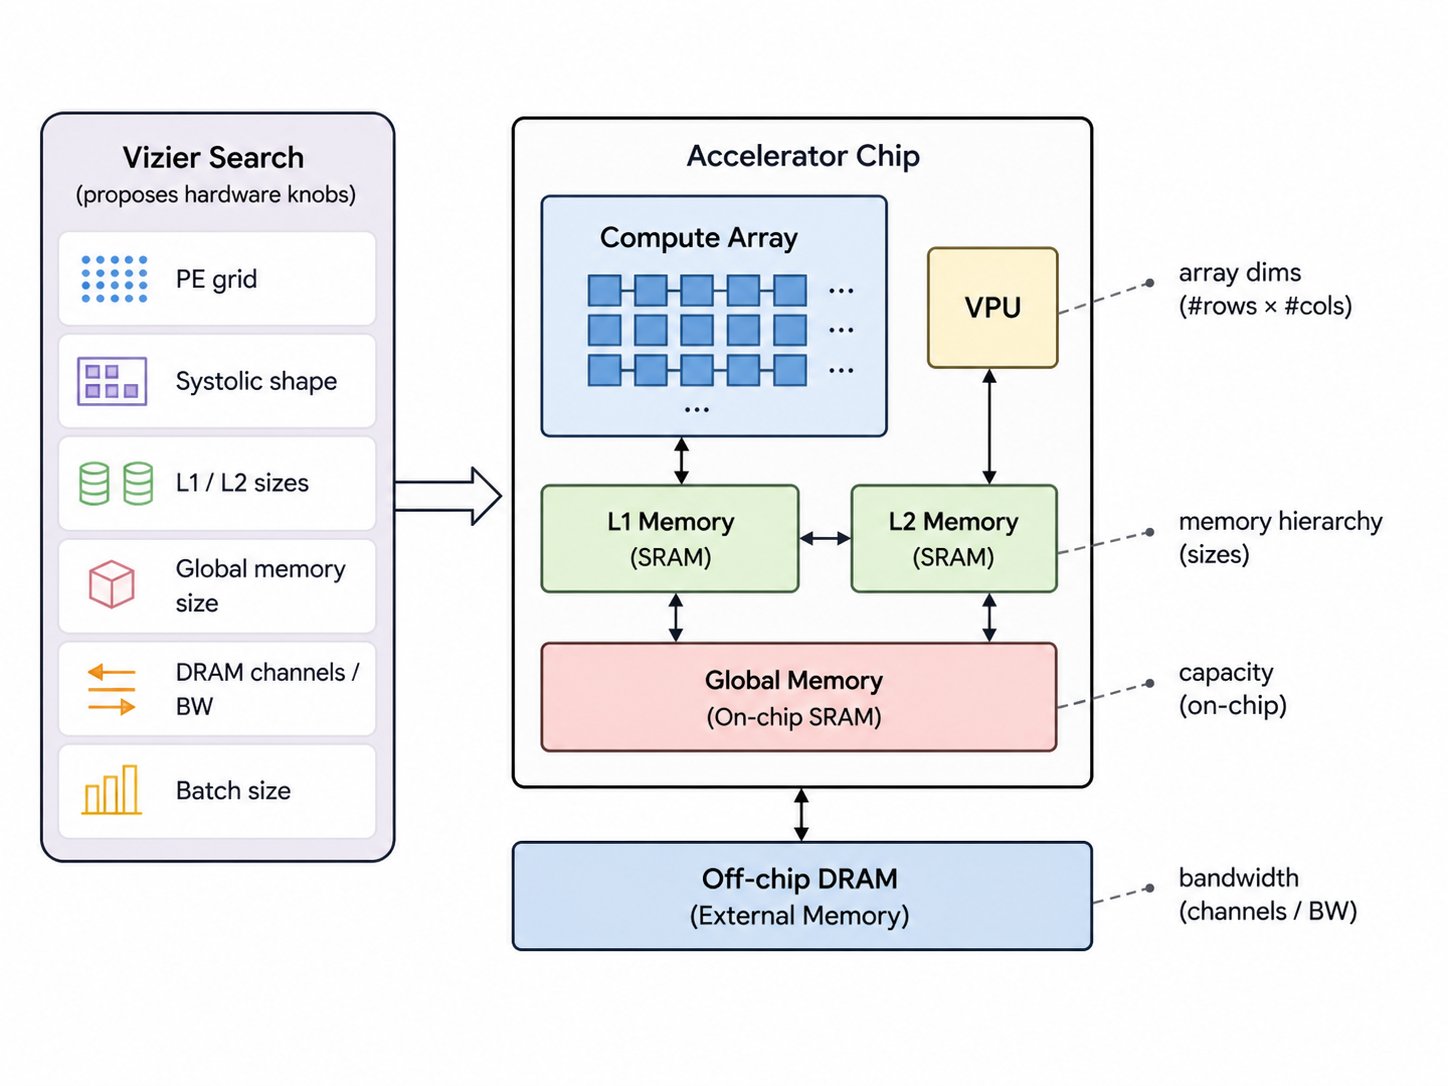
\includegraphics[width=0.5\linewidth]{figs/hardware_layout.png}
% %     \caption{The accelerator datapath template. Processing elements (PEs) are arranged in a grid connected by a mesh network. Each PE contains a systolic array for matrix operations, a vector processing unit (VPU) for non-MAC operations, and private or shared L1/L2 memory. A Global Memory serves as the on-chip scratchpad shared across all PEs. FAST-CORGI jointly optimizes how operations are tiled across this memory hierarchy and which tensors are pinned in Global Memory, replacing the sequential tiling$\rightarrow$fusion pipeline of FAST.}
% %     \label{fig:pipeline}
% % \end{figure}
% % FAST designs inference accelerators by jointly searching over hardware datapaths, software schedules, and compiler passes.
% % It targets a general ML accelerator template (Figure~\ref{fig:pipeline}) consisting of a grid of processing elements (PEs), each containing a systolic array for matrix operations and a vector processing unit (VPU) for non-MAC operations such as softmax and layer normalization.
% % The memory hierarchy includes per-PE L1 scratchpads, optional L2 buffers, a shared Global Memory, and off-chip DRAM.
% % The full hardware configuration is defined by 16 hyperparameters---PE grid dimensions, systolic array sizes, buffer capacities, DRAM channels, and batch size---spanning a datapath search space of $\mathcal O(10^{13})$ \citep[Table~3]{zhang_fast}.

% % FAST operates as a three-stage sequential pipeline within each trial of Google's Vizier:
% % (1)~Vizier proposes a hardware configuration;
% % (2)~Timeloop~ finds the best tiling and mapping for each operation independently, given the fixed hardware, producing per-operation execution time estimates;
% % (3)~an integer linear program (ILP) decides which tensors to pin in the Global Memory to reduce DRAM traffic, given the fixed per-operation schedules.
% % The predicted Perf/TDP is returned to Vizier, which proposes the next configuration.
% % This cycle repeats for ${\sim}5000$ trials.

% % FAST-generated accelerators achieve $3.7\times$ average Perf/TDP improvement over TPU-v3 across vision and NLP workloads~\citep[Section~6.2]{zhang_fast}.
% % However, the sequential decomposition means each stage commits to decisions that downstream stages cannot revise---Timeloop optimizes each operation's tiling without considering how its working-set size affects fusion feasibility, and the fusion ILP cannot request alternative tilings that might enable better global solutions.
% % Our work addresses this limitation by replacing stages~(2) and~(3) with a joint LP formulation.

% % \subsection{Related work.}
% \paragraph{Accelerator design space.} Hardware/Software (HW/SW) design exploration has been widely studied through tools
% that optimize datapath configurations and operation mappings, including
% Eyeriss~\citep{chen2019eyerissv2flexibleaccelerator},
% Timeloop~\citep{timeloop},
% MAESTRO~\citep{kwon2020understandingreuseperformancehardware},
% Interstellar~\citep{yang_interstellar},
% CoSA~\citep{huang2021cosaschedulingconstrainedoptimization},
% and ZigZag~\citep{mei2021zigzag}.
% FAST advanced the field by presenting a tractable way to comprehensively search over datapath,
% schedule, and compiler passes. This demonstrated the potential of co-design to achieve speedups for targeted neural network workloads that can achieve $3.7\times$ Perf/TDP improvement over a standard TPU-v3 baseline.
% However, within single trial involves a sequential flow through 3 components(Vizier for hardware candidate proposal, Timeloop for tiling, and and ILP solver for fusion), for a total of 5000 trials which may take days.
% This imitates the standard human engineering sequential pipeline of designing domain optimized deep learning accelerators---each stage consumes the previous
% stage's output as fixed. Tiling and fusion have mature but separate
% literatures: tiling builds on loop optimization techniques from
% Halide~\citep{ragan2013halide} and Ansor~\citep{zheng2023ansorgeneratinghighperformancetensor},
% while fusion extends compiler passes in XLA and training-time
% rematerialization~\citep{chen2016trainingdeepnetssublinear,
% jain2020checkmatebreakingmemorywall}. Recent work has begun to address joint tiling and fusion optimization:
% TileFlow \citep{zheng2023tileflow} explores fusion dataflows via tree-based
% analysis, and FADiff \citep{jia2025fadifffusionawaredifferentiableoptimization} formulates a differentiable
% joint mapping-fusion objective. Our formulation differs in targeting hardware-software
% co-design with a large-scale LP that provides valid lower bounds via exact
% bilinear linearization, and additionally handles rematerialization
% and dynamic memory scheduling for datacenter-scale accelerators.

% \paragraph{Optimization Techniques.} Our joint LP reformulation is enabled by McCormick
% envelopes~\citep{mccormick1976computability}, which exactly linearize
% the bilinear tiling$\times$placement interaction, and by scalable first-order
% LP solvers descended from PDLP~\citep{applegate2022practicallargescalelinearprogramming}.
% For the outer hardware search loop, we draw on recent work using LLMs as
% informed mutation operators---FunSearch~\citep{romera2024mathematical},
% AlphaEvolve~\citep{novikov2025alphaevolvecodingagentscientific}, and
% EvoPrompting~\citep{chen2023evopromptinglanguagemodelscodelevel}---to
% propose hardware configurations guided by workload bottleneck analysis and prior trial results.
% A full discussion of related work appears in Appendix~\ref{related_work_appendix}.
% % \subsection{Related Work}
% % \paragraph{Accelerator design space exploration.}
% % Hardware ML accelerators are characterized by their datapath (compute units, memory hierarchy, interconnect) and software schedule (how operations map onto hardware).
% % A substantial body of work explores design spaces of accelerator families by mutating datapath hyperparameters and operation mappings.
% % % Eyeriss
% % \citep{chen2019eyerissv2flexibleaccelerator} introduced Eyeriss, a spatial architecture with a row-stationary dataflow for energy-efficient CNNs.
% % % Timeloop
% % \citep{timeloop} proposed Timeloop, a systematic infrastructure for evaluating DNN accelerator schedules and datapaths.
% % % MAESTRO
% % \citep{kwon2020understandingreuseperformancehardware} developed MAESTRO, a data-centric framework for understanding DNN mapping performance.
% % % Interstellar
% % \citep{yang_interstellar} used Halide's scheduling language to analyze DNN accelerators in Interstellar.
% % % dMazeRunner
% % \citep{dave2019dmazerunner} optimized convolution mappings on dataflow accelerators with dMazeRunner. 
% % % MAGNet
% % \citep{venkatesan2019magnet} proposed MAGNet, a modular accelerator generator, reporting up to 1.75$\times$ Perf/W improvement.
% % % Apollo
% % \citep{yazdanbakhsh2021apollotransferablearchitectureexploration} explored transferable architecture exploration via Apollo.
% % % ConfuciuX
% % \citep{kao2020confuciuxautonomoushardwareresource} applied reinforcement learning to hardware resource assignment.
% % % CoSA
% % Huang \etal~formulated accelerator mapping as a constrained optimization problem in CoSA \citep{huang2021cosaschedulingconstrainedoptimization}.
% % FAST extended these approaches by jointly optimizing datapath, schedule, and compiler passes including operation fusion, achieving $3.7\times$ average Perf/TDP improvement over TPU-v3 across vision and language workloads.
% % Our work preserves FAST's outer hardware search loop but replaces the sequential inner optimization with a joint linear program.


% % \paragraph{Operation fusion and memory optimization.}
% % Operation fusion reduces DRAM traffic by keeping intermediate tensors on-chip.
% % Production compilers such as XLA fuse simple patterns, but each fusion region contains at most one matrix operation.
% % FAST introduced an ILP-based fusion technique that pins activation and weight tensors in Global Memory to minimize total execution time, but with a static placement model restricted to consecutively-executed operations.
% % % Rematerialization / checkpointing
% % Rematerialization---recomputing values instead of storing them---is well-studied in the context of training memory optimization.
% % \citep{chen2016trainingdeepnetssublinear} proposed gradient checkpointing to trade compute for memory during backpropagation.
% % \citep{jain2020checkmatebreakingmemorywall} formulated optimal checkpointing as an ILP.
% % Our \textcolor{skyblue}{V0} formulation adapts rematerialization to the inference setting.

% % \paragraph{Joint optimization and linearization techniques.}
% % The interaction between tiling decisions and fusion opportunities is a bilinear optimization problem: execution time depends on the product of tiling selection and tensor placement variables.
% % McCormick envelopes provide exact linearization of bilinear terms over box-constrained domains by introducing auxiliary variables and four linear constraints per product term.
% % The foundational work by McCormick established convex underestimators for factorable nonconvex programs \citep{mccormick1976computability}.
% % % % McCormick 1976
% % % (McCormick, ``Computability of Global Solutions to Factorable Nonconvex Programs,'' \textit{Mathematical Programming}, 1976).
% % Our \textcolor{skyblue}{V1} formulation applies McCormick linearization to the tiling $\times$ placement interaction, enabling exact reformulation as a LP.
% % % PDLP
% % \citep{applegate2022practicallargescalelinearprogramming} developed PDLP, a practical first-order method for large-scale LP solving that scales to instances with billions of nonzeros, based on which we build our variant of LP solver that empowers solving the system \textcolor{skyblue}{V0} and \textcolor{skyblue}{V1} LPs efficiently.

% % % Our LP instances (15--25M nonzeros for EfficientNet-B7) are well within the capacity of such solvers.

% % \paragraph{Tiling and loop optimization.}
% % Optimal tiling for nested loop computations has been studied extensively in the compiler community.
% % % Halide
% % \citep{ragan2013halide} introduced Halide, a language for optimizing parallelism and locality in image processing pipelines.
% % % TVM / Ansor
% % \citep{zheng2023ansorgeneratinghighperformancetensor} proposed Ansor, which generates high-performance tensor programs via hierarchical search.
% % % ZigZag
% % Mei \etal~enlarged the joint architecture-mapping design space for DNN accelerators in ZigZag \citep{mei2021zigzag}.
% % These works optimize tiling for fixed hardware; our contribution is to co-optimize tiling with fusion decisions.

% % % \paragraph{Neural architecture and hardware co-design.}
% % % Co-optimizing neural network architectures and their target hardware has gained attention.
% % % % MnasNet
% % % Tan \etal~performed platform-aware neural architecture search
% % % (\url{https://arxiv.org/abs/1807.11626}).
% % % % Once-for-All
% % % Cai \etal~proposed Once-for-All networks that decouple training from deployment
% % % (\url{https://arxiv.org/abs/1908.09791}).
% % % % Hardware-aware NAS
% % % Zhou \etal~rethought co-design of neural architectures and hardware accelerators
% % % (\url{https://arxiv.org/abs/2102.08619}).
% % % While our framework does not modify the neural network architecture, the joint LP formulation could naturally extend to include architecture decisions as additional variables.

% % \paragraph{LLM-guided optimization and scientific discovery.}
% % Recent work has demonstrated that large language models can serve as effective mutation operators in evolutionary search.
% % % FunSearch
% % Romera-Paredes \etal~introduced FunSearch, pairing a pretrained LLM with an evaluator to discover new solutions to open mathematical problems \citep{romera2024mathematical}.
% % % AlphaEvolve
% % \citep{novikov2025alphaevolvecodingagentscientific} presented AlphaEvolve, an evolutionary coding agent powered by Gemini that discovered improved algorithms for data center scheduling, chip design, and matrix multiplication.
% % % EvoPrompting
% % Chen \etal~proposed EvoPrompting, combining evolutionary search with LLM-based code generation for neural architecture discovery \citep{chen2023evopromptinglanguagemodelscodelevel}.
% % Our LLM-guided hardware search draws on these ideas, using an LLM to propose hardware configurations informed by workload analysis and prior trial outcomes, while the joint LP provides rigorous inner-loop optimization.

% % \paragraph{Datacenter accelerator economics.}
% % The economic viability of specialized accelerators depends on deployment scale.
% % % ASIC Clouds
% % \citep{magaki2016asic,xie2018extreme}~analyzed specialization economics under total cost of ownership.
% % % TPUv4i
% % \citep{jouppi2021ten} distilled lessons from three generations of TPU design.
% % FAST provided ROI analysis showing that specialized accelerators can be profitable with deployments of $2,000$--$4,000$ units.
% % Our joint optimization targets the same deployment regime, but achieves better Perf/TDP through the larger effective search space of joint tiling-fusion optimization.

% page edit

\section{Related Work}
\label{sec:related}

Hardware and software design exploration has been studied through tools that optimize datapath configurations and operation mappings, including
Eyeriss~\citep{chen2019eyerissv2flexibleaccelerator},
Timeloop~\citep{timeloop},
MAESTRO~\citep{kwon2020understandingreuseperformancehardware},
Interstellar~\citep{yang_interstellar},
CoSA~\citep{huang2021cosaschedulingconstrainedoptimization},
and ZigZag~\citep{mei2021zigzag}.
For LLM serving specifically, LLMCompass~\citep{zhang2024llmcompass} provides a fast analytical hardware-evaluation framework for design-space exploration, but treats mapping and scheduling as enumeration over a hardware template rather than as decisions inside an optimization program.
FAST~\citep{zhang_fast} advanced the field with a full-stack search over datapath, schedule, and compiler passes, achieving $3.7\times$ Perf/TDP over TPU-v3, but its sequential pipeline (Vizier$\to$Timeloop$\to$ILP) requires ${\sim}5{,}000$ trials and precludes cross-stage trade-offs.
Recent work has begun addressing joint tiling-fusion:
TileFlow~\citep{zheng2023tileflow} explores fusion dataflows via tree-based analysis, and FADiff~\citep{jia2025fadifffusionawaredifferentiableoptimization} formulates a differentiable joint mapping-fusion objective. Our formulation differs in targeting HW/SW co-design with a large-scale LP that provides valid lower bounds via tight McCormick relaxation exact at integral tiling/placement decisions, and additionally handles rematerialization and dynamic memory scheduling.
Polyhedral compilation~\citep{feautrier1992affine,bondhugula2008pluto,baghdadi2019tiramisu} reasons jointly about tiling and fusion as affine loop transformations for fixed hardware, and fusion-conflict-graph methods~\citep{acharya2020fusion} cast fusion partitioning as graph optimization; none model time-varying buffer residency, eviction, or rematerialization as scheduling decisions, and hardware parameters are never decision variables. Conversely, execution \emph{reordering}, the core strength of the polyhedral model, is the one axis we fix: the topological order is an input (Definition~\ref{def:seq_scope}), and making order a decision above the LP is future work.
Our joint LP is enabled by McCormick envelopes~\citep{mccormick1976computability}, and scalable first-order LP solvers descended from PDLP~\citep{applegate2022practicallargescalelinearprogramming}. For outer-loop search, we draw on LLMs as informed mutation operators such as FunSearch~\citep{romera2024mathematical}, AlphaEvolve~\citep{novikov2025alphaevolvecodingagentscientific}, and EvoPrompting~\citep{chen2023evopromptinglanguagemodelscodelevel}, to propose hardware configurations guided by workload bottleneck analysis. A full discussion appears in Appendix~\ref{related_work_appendix}.
% % % \section{Methodology}
% % % \label{sec:methods}

% % % We present the CHEETAH (\acroletter{C}o-designed \acroletter{H}ardware \acroletter{E}xploration via \acroletter{E}fficient \acroletter{T}hroughput and \acroletter{H}ybrid-search) framework in three parts: Section~\ref{sec:v0} introduces CHEETAH-V0, which extends the static fusion ILP with time-indexed placement and rematerialization. Section~\ref{sec:v1} presents CHEETAH-V1, which jointly optimizes tiling and fusion via McCormick linearization. Section~\ref{sec:llm_outer} describes the LLM-Architect outer loop.


% % % % \subsection{\Vzero~: Multi-Period Placement with Rematerialization}
% % % \subsection{CHEETAH-V0: Multi-Period Placement with Rematerialization}
% % % \label{sec:v0}

% % % Our first extension models the neural network's execution as a sequence of $T$ discrete timesteps (one per operation in execution order). This decides at which time, which tensor is pinned, evicted, or recomputed to optimally minimize cycle counts. The key features are:

% % % \paragraph{Time-indexed placement.}
% % % Instead of a single binary $p_i^k$ per tensor, we introduce $p_{i,t}^k \in [0,1]$ for each tensor $k$ of layer $i$ at each timestep $t$. A tensor can be pinned at timestep $t=5$, and evicted at $t=10$. This models a dynamic memory manager within a single inference pass.

% % % \paragraph{Rematerialization.}
% % % Rather than always paying DRAM bandwidth to reload an evicted tensor, we introduce variables $r_{i,t} \in [0,1]$ indicating that layer $i$ is recomputed at timestep $t$ to restore its output to the Global Buffer. This is particularly valuable for models such as EfficientNet, where depthwise convolutions account for only ${\sim}5\%$ of total FLOPs but produce large activation tensors. Recomputing a depthwise layer to avoid re-reading 6\,MiB from DRAM at 256\,GB/s can be faster than the DRAM reload itself.

% % % \paragraph{Relaxed skip-connection handling.}
% % % We lift the limitation of our baseline original ILP, which restricts activation pinning to consecutively-executed operations and limits multi-fanout nodes so that at most one consumer benefits from on-chip data. CHEETAH-V0 uses edge-indexed placement variables $p_{e,t}$ for each edge $e \in \mathcal{E}$ of the dataflow graph, correctly modeling the case where one consumer of a skip connection benefits from on-chip data while another does not.

% % % The CHEETAH-V0 LP formulation is:
% % % \begin{equation}
% % % % \label{eq:v0}
% % % \begin{aligned}
% % % \min \quad & \sum_{i \in \mathcal{N}} T_i + \sum_{i \in \mathcal{N}} \sum_{t \in \mathcal{T}} c_i^{\text{remat}} \, r_{i,t} \\
% % % \text{s.t.} \quad
% % % & T_i \geq \Tmax_i - \sum_{k \in \{I,O,W\}} t_i^k \cdot p_{i,o(i)}^k & \forall\, i \in \mathcal{N} \\
% % % & T_i \geq \Tmin_i & \forall\, i \in \mathcal{N} \\
% % % & \sum_{i \in \mathcal{N}} \sum_{k} d_i^k \, p_{i,t}^k \leq \CGM & \forall\, t \in \mathcal{T} \\
% % % & p_{i,t}^k \leq p_{i,t-1}^k + r_{i,t} & \forall\, i, t, k \in \{I,O\} \\
% % % & p_{i,t}^W \leq p_{i,t-1}^W & \forall\, i, t \\
% % % & r_{i,t} = 0 & \forall\, i, t \leq o(i) \\
% % % & 0 \leq p_{i,t}^k, r_{i,t} \leq 1 &
% % % \end{aligned}
% % % \tag{V0}\label{eq:v0}
% % % \end{equation}


% % % where $o(i)$ is the execution order of operation $i$, $d_i^k$ is the byte size of tensor $k$ for layer $i$, and $c_i^{\text{remat}}$ is the recomputation cost.

% % % \paragraph{Variable and constraint digest.}
% % % The V0 objective minimizes the sum of execution times $\sum_i T_i$ and
% % % rematerialization costs $c_i^{\text{remat}}\, r_{i,t}$.
% % % Per-operation latency $T_i$ is lower-bounded by the physical on-chip
% % % floor $T_i^{\min}$ and the off-chip time $T_i^{\max}$ adjusted for DRAM
% % % savings $t_i^k \cdot p_{i,o(i)}^k$ from pinned tensors.
% % % Placement variables $p_{i,t}^k \in [0,1]$ track Global Memory residency
% % % for inputs, outputs, and weights at each timestep, subject to a global
% % % capacity constraint $C_{\text{GM}}$. Persistence is governed by $p_{i,t}^k \;\leq\; p_{i,t-1}^k + r_{i,t},$ enforcing that activations are either resident from the previous timestep
% % % or recomputed; weight tensors satisfy the stricter monotone constraint
% % % $p_{i,t}^W \leq p_{i,t-1}^W$, as weights cannot be rematerialized.
% % % Rematerialization $r_{i,t}$ is only permitted post-execution
% % % ($t > o(i)$) and requires on-chip availability of both inputs and
% % % weights.
% % % For DeepSeek-V3 ($L \approx 6{,}300$), this formulation yields a
% % % large-scale program with approximately 3.3M variables and 3.7M
% % % constraints.


% % % % \subsection{\textcolor{skyblue}{V1}: Joint Tiling and Fusion via McCormick Linearization}
% % % \subsection{CHEETAH-V1: Joint Tiling and Fusion via McCormick Linearization}
% % % \label{sec:v1}

% % % \begin{wrapfigure}{r}{0.2\linewidth}
% % %     \vspace{-12pt}
% % %     \centering
% % %     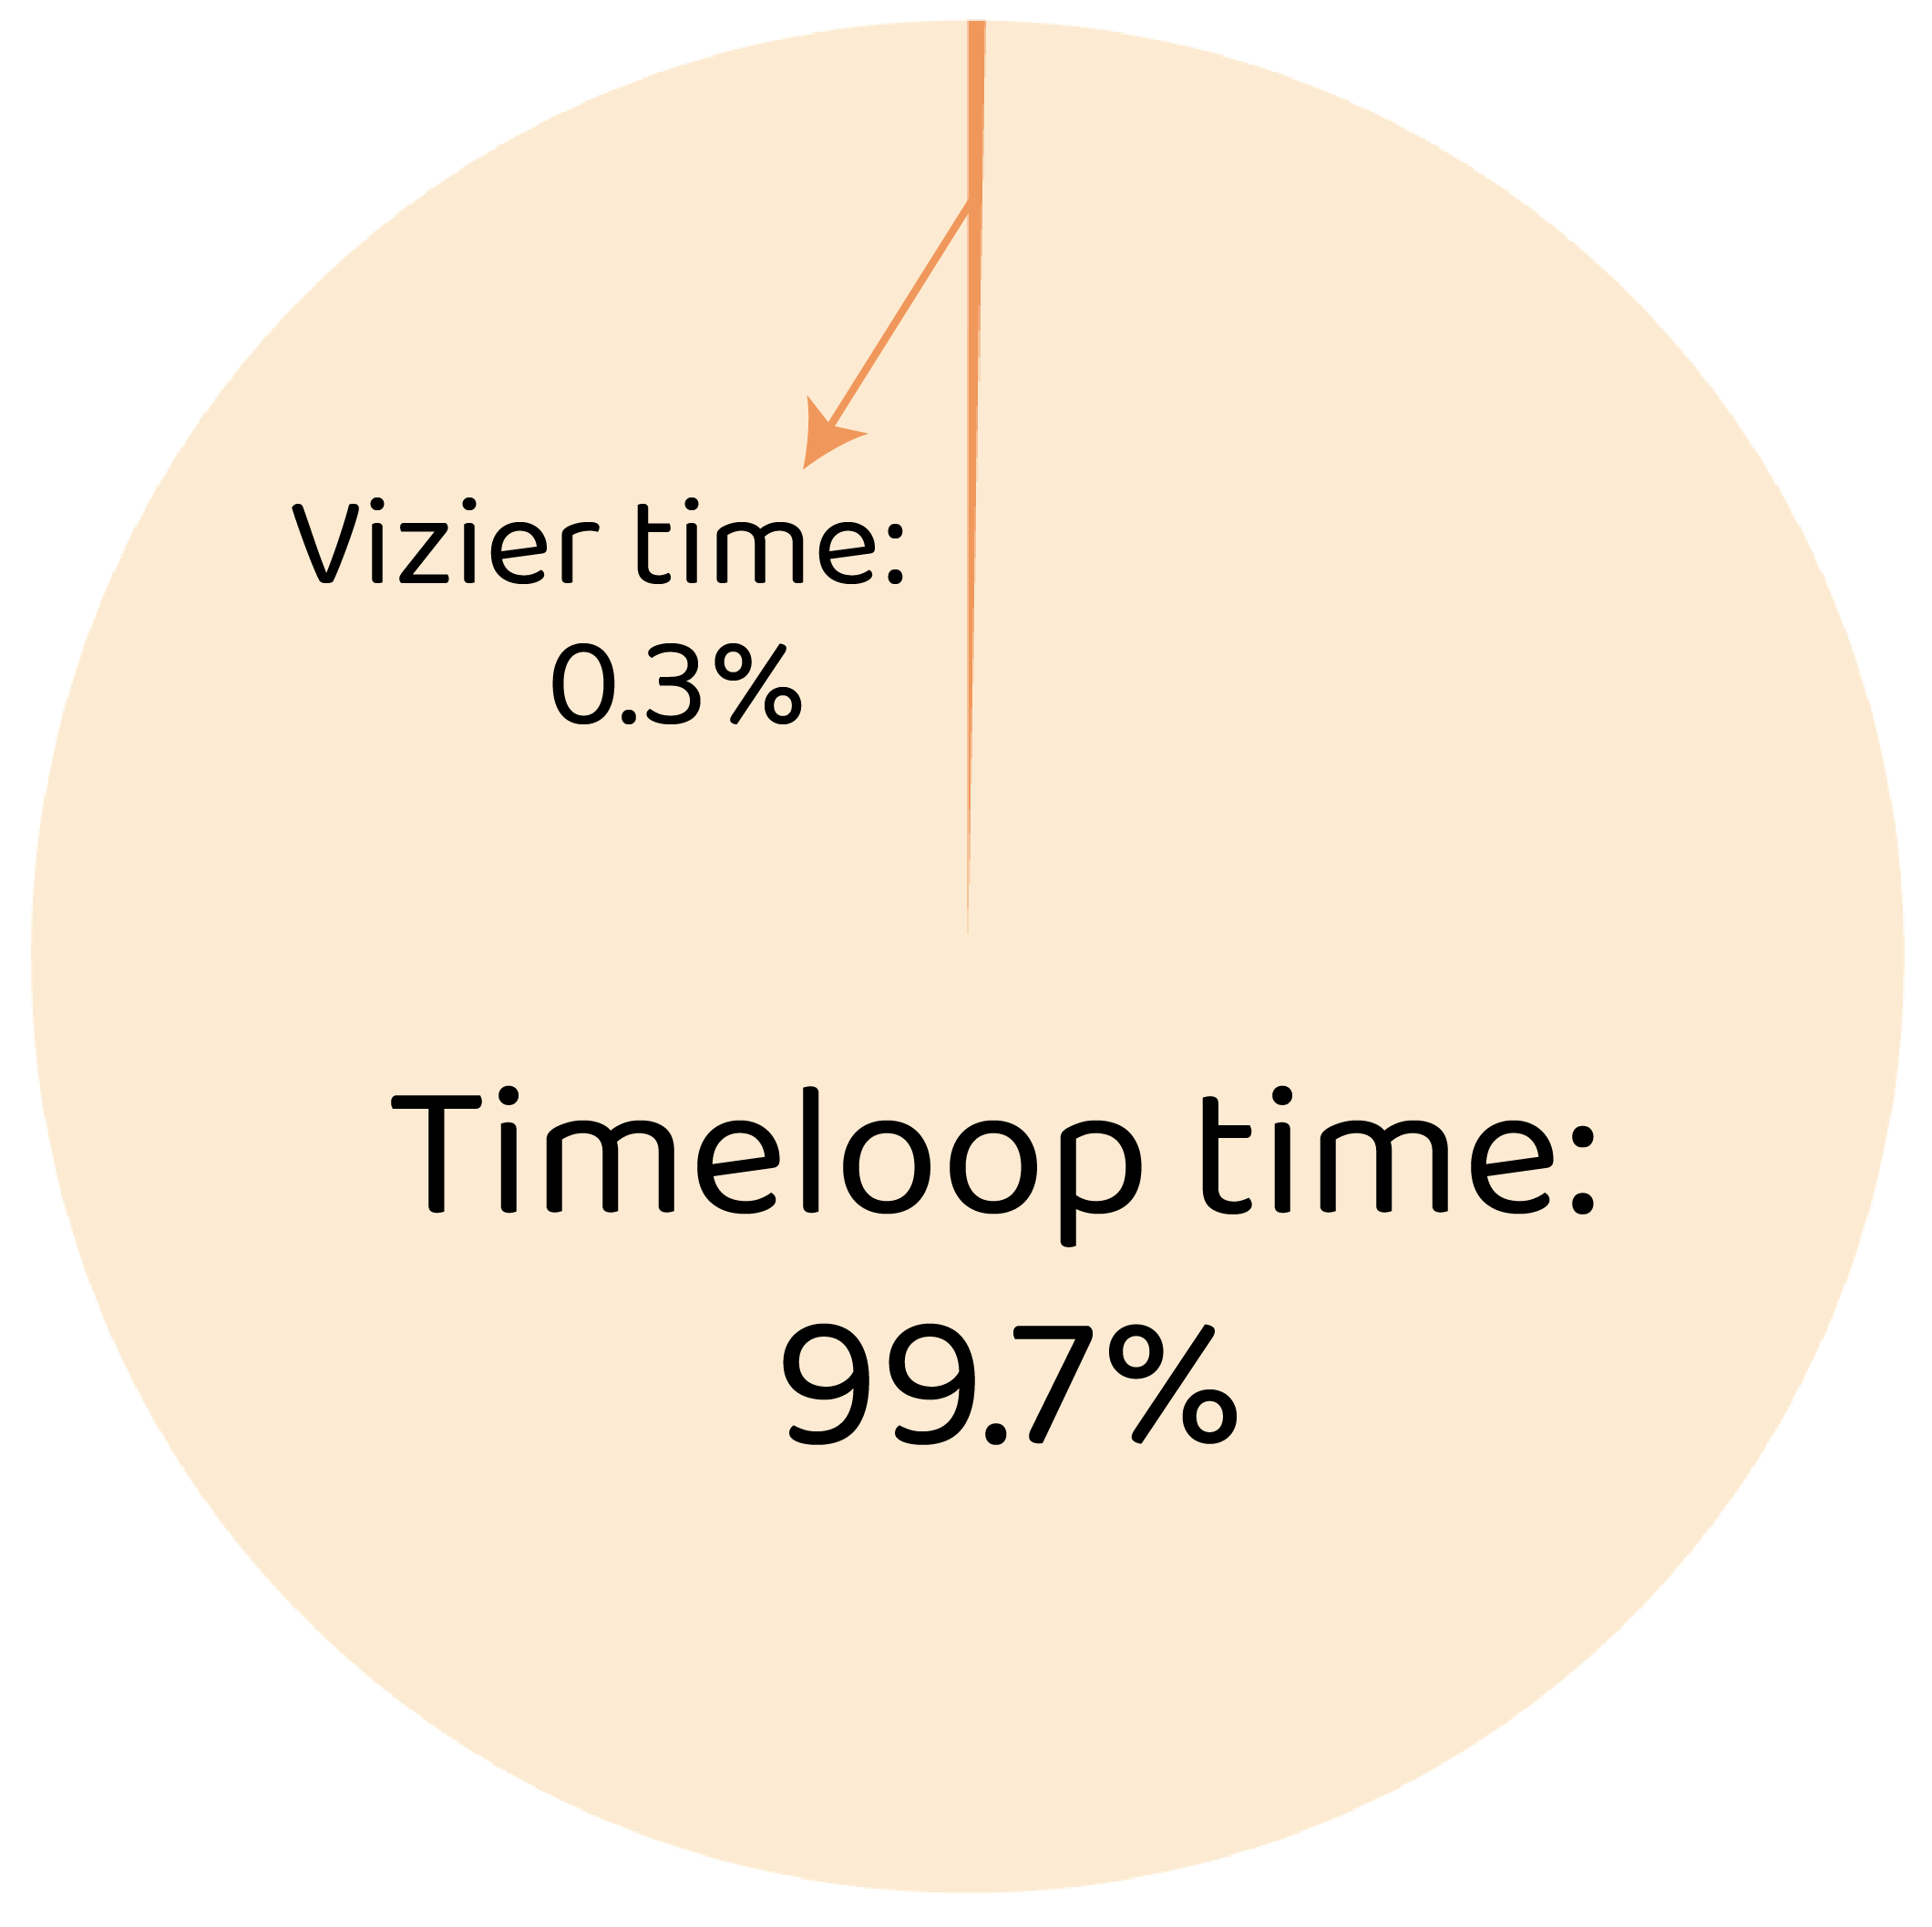
\includegraphics[width=\linewidth]{fig3/timeloop_vs_vizier.png}
% % %     \caption{Per-trial wall-clock breakdown.}
% % %     \label{fig:timeloop-time}
% % %     \vspace{-10pt}
% % % \end{wrapfigure}
% % % Despite V0's improvements, it inherits the sequential dependence on external tiling tools (e.g., Timeloop) because it lacks a linear expression for non-linear tiling-fusion interactions. As shown in Figure~\ref{fig:timeloop-time}, Timeloop accounts for over 99\% of per-trial latency, creating a prohibitive bottleneck for multi-thousand-trial searches. To resolve this, CHEETAH-V1 internalizes tiling by precomputing Pareto-pruned configurations and encoding them as decision variables. This removes Timeloop from the critical path, collapsing each trial to a single Vizier-proposal and LP-solve step. We start with introducing the preprocessing stage below before presenting the full formulation in Section~\ref{sec::v1}.

% % % % The limitations of prior work is still inherited in the V0 formulation due to the difficulty of expressing non-linear relationships as linear constraints. Therefore tiling decisions $(\Tmax_i, \Tmin_i, t_i^k)$ are fixed constants provided by additional software, such as Timeloop. A natural question is whether this sequential dependence also creates a \emph{runtime} bottleneck. Figure~\ref{fig:timeloop-time} confirms that it does: across different models, Timeloop scheduling on average accounts for over 99\% of per-trial wall-clock time, while the Vizier proposal and fusion ILP together consume less than 1\% on average. Because the outer loop requires thousands of trials to converge, the cumulative cost of repeated Timeloop invocations dominates the total search budget. This observation motivates a key design choice in CHEETAH-V1: rather than calling Timeloop online during each trial, we precompute a Pareto-pruned set of tiling configurations once (Section~\ref{sec:pareto}) and encode the tiling selection as decision variables \emph{inside} the LP. This eliminates Timeloop from the per-trial critical path entirely, reducing each trial to a single Vizier-proposal$\,\to\,$LP-solve step.

% % % % CHEETAH-V1 captures tiling as a \emph{decision variable} inside the LP, enabling the solver to jointly optimize tiling and fusion. We start with describing our preprocessing stage in Section~\ref{sec:pareto} before presenting the full formulation in Section~\ref{sec::v1}.


% % % \paragraph{Pareto Pruning Pre-Pass} The raw tiling search space for a $7$-dimensional convolution loop with $3$ memory levels is $\mathcal O(10^7)$ configurations per operation. We reduce this to a tractable Pareto-optimal subset $\mathcal{C}_i$ for each operation $i$ via a pre-pass for (1) L1 feasibility where configurations whose tiled working set exceeds L1 scratchpad capacity $C_{L1}$ are discarded; (2) Pareto optimality where a configuration $c$ is retained only if no other configuration achieves both lower $\Tmax_i(c)$ \emph{and} smaller working-set size in the Global Buffer.

% % % In practice, Pareto pruning reduces $\mathcal O(10^7)$ raw configurations to $|\mathcal{C}_i| \approx 10^2$ to $10^3$ per operation. Timeloop is run once per (operation, configuration) pair, producing the triple $(\Tmin_i(c), \Tmax_i(c), t_i^k(c))$ for each retained configuration $c \in \mathcal{C}_i$. These are precomputed constants---the LP solver makes no Timeloop calls at solve time.

% % % \paragraph{Time-invariant Pareto fronts.}
% % % A key observation is that the Pareto front shape is invariant to memory time: configurations are ranked by compute cycles and working-set bytes, neither of which depends on bandwidth. Changing bandwidth rescales the DRAM access cost $t_i^k(c)$ uniformly. This means the Pareto-pruned configuration sets can be precomputed \emph{once} and reused across all Vizier trials that share the same compute configuration class, amortizing the expensive Timeloop precomputation.

% % % \subsubsection{The Joint CHEETAH-V1 LP Formulation}\label{sec::v1}

% % % \paragraph{From fixed constants to decision variables.}
% % % In static and V0 formulations, Timeloop selects a single tiling per operation externally and passes the results to the LP as fixed constants $\Tmax_i$, $\Tmin_i$, $t_i^k$. The DRAM savings from pinning tensor $k$ of operation $i$ is then simply $t_i^k \cdot p_{i,o(i)}^k$---a constant times a variable, which is already linear. V1 brings this tiling choice \emph{inside} the LP by introducing \textbf{tiling selection variables} $y_{i,c} \in [0,1]$, one per Pareto-optimal configuration $c \in \mathcal{C}_i$ from the pre-pass, with the constraint $\sum_c y_{i,c} = 1$ (exactly one configuration is selected per operation). The Timeloop-precomputed constants $\Tmax_i(c)$, $\Tmin_i(c)$, $t_i^k(c)$ now become \emph{per-configuration coefficients} indexed by $c$. This means the DRAM savings term becomes $t_i^k(c) \cdot y_{i,c} \cdot p_{\text{assoc}(i,k),\, o(i)}$. This is a product of \emph{two} decision variables, which is bilinear and cannot be handled by a convex programming directly.
 
% % % % \paragraph{Linearization via McCormick envelopes.}
% % % % We linearize this product exactly via the classical McCormick substitution. Specifically,  we introduce \textbf{auxiliary variables} $w_{i,c,k} := y_{i,c} \cdot p_{\text{assoc}(i,k),\, o(i)}$ that represent the joint effect of selecting tiling $c$ \emph{and} pinning tensor $k$, constrained by:
% % % % \begin{equation}
% % % % \label{eq:mccormick}
% % % % \begin{aligned}
% % % %     w_{i,c,k} &\leq y_{i,c}, \qquad
% % % %     w_{i,c,k} \leq p_{\text{assoc}(i,k),\, o(i)} \\
% % % %     w_{i,c,k} &\geq y_{i,c} + p_{\text{assoc}(i,k),\, o(i)} - 1, \qquad
% % % %     w_{i,c,k} \geq 0
% % % % \end{aligned}
% % % % \end{equation}
% % % % Since both factors lie in $[0,1]$, these four constraints force $w_{i,c,k} = y_{i,c} \cdot p$ at any integer vertex, requiring no manually tuned constants. Together, $y_{i,c}$ and $w_{i,c,k}$ account for 1.6M of the 2.08M variables in the \Vone~ LP (Table~\ref{tab:v1_scale}). \todo{change to MoE?}

% % % \paragraph{Linearization via McCormick envelopes.}
% % % We linearize this product exactly via the classical McCormick substitution \citep{mccormick1976computability}. Specifically, we introduce \textbf{auxiliary variables} $w_{i,c,k} := y_{i,c} \cdot p_{\text{assoc}(i,k),\, o(i)}$ that represent the joint effect of selecting tiling $c$ \emph{and} pinning tensor $k$, constrained by:
% % % \begin{equation}
% % % \label{eq:mccormick}
% % % \begin{aligned}
% % %     w_{i,c,k} &\leq y_{i,c}, \qquad
% % %     w_{i,c,k} \leq p_{\text{assoc}(i,k),\, o(i)} \\
% % %     w_{i,c,k} &\geq y_{i,c} + p_{\text{assoc}(i,k),\, o(i)} - 1, \qquad
% % %     w_{i,c,k} \geq 0
% % % \end{aligned}
% % % \end{equation}
% % % Since both factors lie in $[0,1]$, these four constraints force $w_{i,c,k} = y_{i,c} \cdot p$ at any integer vertex, requiring no manually tuned constants. Together, $y_{i,c}$ and $w_{i,c,k}$ constitute the majority of V1's decision variables (Table~\ref{tab:v1_scale}).
 

% % % % \paragraph{Full formulation.}
% % % % Combining tiling selection, time-indexed placement, rematerialization, and McCormick linearization, the full V1  formulation is:

% % % % \begin{equation}
% % % % % \label{eq:v1}
% % % % \begin{aligned}
% % % % \min \quad & \sum_{i \in \mathcal{N}} T_i + \sum_{i \in \mathcal{N}} \sum_{t \in \mathcal{T}} c_i^{\text{remat}} \, r_{i,t} \\[4pt]
% % % % \text{s.t.} \quad
% % % % & \sum_{c \in \mathcal{C}_i} y_{i,c} = 1 & \forall\, i \in \mathcal{N} \\[3pt]
% % % % & T_i \geq \sum_{c \in \mathcal{C}_i} \Tmax_i(c)\, y_{i,c} - \sum_{c \in \mathcal{C}_i} \sum_{k} t_i^k(c)\, w_{i,c,k} & \forall\, i \in \mathcal{N} \\[3pt]
% % % % & T_i \geq \sum_{c \in \mathcal{C}_i} \Tmin_i(c)\, y_{i,c} & \forall\, i \in \mathcal{N} \\[3pt]
% % % % & w_{i,c,k} \leq y_{i,c} & \forall\, i, c, k \\
% % % % & w_{i,c,k} \leq p_{\text{assoc}(i,k),\, o(i)} & \forall\, i, c, k \\
% % % % & w_{i,c,k} \geq y_{i,c} + p_{\text{assoc}(i,k),\, o(i)} - 1 & \forall\, i, c, k \\[3pt]
% % % % & \sum_{e \in \mathcal{E}} d_e\, p_{e,t} + \sum_{i \in \mathcal{N}} d_i^W\, p_{i,t}^W \leq \CGM & \forall\, t \in \mathcal{T} \\[3pt]
% % % % & p_{e,t} \leq p_{e,t-1} + r_{\text{src}(e),\, t} & \forall\, e, t > o(\text{src}(e)) \\
% % % % & p_{i,t}^W \leq p_{i,t-1}^W & \forall\, i, t > o(i) \\[3pt]
% % % % & r_{i,t} = 0 & \forall\, i, t \leq o(i) \\
% % % % & r_{i,t} \leq p_{e,t} & \forall\, e \in \text{in}(i), t > o(i) \\
% % % % & r_{i,t} \leq p_{i,t}^W & \forall\, i, t > o(i) \\[3pt]
% % % % & T_i, p_{e,t}, p_{i,t}^W, r_{i,t}, w_{i,c,k} \geq 0 &
% % % % \end{aligned}
% % % % \tag{\textcolor{skyblue}{V1}}\label{eq:v1}
% % % % \end{equation}
% % % % full formulation below in appendix 
% % % % \begin{equation}
% % % % \begin{aligned}
% % % % \min \quad & \sum_{i \in \mathcal{N}} T_i + \sum_{i \in \mathcal{N}} \sum_{t \in \mathcal{T}} c_i^{\text{remat}} \, r_{i,t} \\[4pt]
% % % % \text{s.t.} \quad
% % % % & \sum_{c \in \mathcal{C}_i} y_{i,c} = 1 & \forall\, i \in \mathcal{N} \\[3pt]
% % % % & T_i \geq \max\!\left(\sum_{c \in \mathcal{C}_i} \Tmin_i(c)\, y_{i,c},\;\; \sum_{c \in \mathcal{C}_i} \Tmax_i(c)\, y_{i,c} - \sum_{c \in \mathcal{C}_i} \sum_{k} t_i^k(c)\, w_{i,c,k}\right) & \forall\, i \in \mathcal{N} \\[3pt]
% % % % & w_{i,c,k} \leq y_{i,c}, \quad w_{i,c,k} \leq p_{\text{assoc}(i,k),\, o(i)}, \quad w_{i,c,k} \geq y_{i,c} + p_{\text{assoc}(i,k),\, o(i)} - 1 & \forall\, i, c, k \\[3pt]
% % % % & \sum_{e \in \mathcal{E}} d_e\, p_{e,t} + \sum_{i \in \mathcal{N}} d_i^W\, p_{i,t}^W \leq \CGM & \forall\, t \in \mathcal{T} \\[3pt]
% % % % & p_{e,t} \leq p_{e,t-1} + r_{\text{src}(e),\, t} & \forall\, e,\, t > o(\text{src}(e)) \\
% % % % & p_{i,t}^W \leq p_{i,t-1}^W & \forall\, i,\, t > o(i) \\[3pt]
% % % % & r_{i,t} = 0 \;\; \forall\, t \leq o(i); \quad r_{i,t} \leq \min\!\big(p_{e,t},\, p_{i,t}^W\big) \;\; \forall\, e \in \text{in}(i),\, t > o(i) \\[3pt]
% % % % & T_i,\, p_{e,t},\, p_{i,t}^W,\, r_{i,t},\, w_{i,c,k} \geq 0 &
% % % % \end{aligned}
% % % % \tag{\textcolor{skyblue}{V1}}\label{eq:v1}
% % % % \end{equation}

% % % \paragraph{Variable and constraint digest.}
% % % The V1 formulation inherits all the features of the V0 formulation, and additionally captures tiling by introducing selection variables
% % % $y_{i,c} \in [0,1]$, constrained by $\sum_c y_{i,c} = 1$, to choose
% % % from $|\mathcal{C}_i|$ Pareto-optimal configurations.
% % % Each configuration defines compute costs $T_i^{\max}(c)$,
% % % $T_i^{\min}(c)$, and per-tensor DRAM savings $t_i^k(c)$.
% % % We linearize the resulting bilinear DRAM-savings term exactly via
% % % McCormick auxiliary variables $w_{i,c,k}$, which enforce $w_{i,c,k} \;=\; y_{i,c} \cdot p_{\mathrm{assoc}(i,k),\,o(i)}$ at integer vertices without a relaxation gap.

% % % Per-operation latency $T_i$ is lower-bounded by the weighted
% % % configuration floor $\sum_c T_i^{\min}(c)\, y_{i,c}$ and the weighted
% % % off-chip cost $\sum_c T_i^{\max}(c)\, y_{i,c}$ minus achievable savings
% % % $\sum_{c,k} t_i^k(c)\, w_{i,c,k}$.
% % % This coupling enables the solver to accept sub-optimal local tiling
% % % (higher $T_i^{\max}$) if its smaller memory footprint unlocks global
% % % fusion gains that outweigh the compute-utilization loss.
% % % Capacity and persistence constraints carry over from V0, utilizing
% % % edge-indexed placement $p_{e,t}$ to handle multi-fanout nodes.
% % % For DeepSeek-V3, the V1 LP scales to approximately $2{,}504{,}019$ variables, $2{,}983{,}450$ constraints, and $6{,}094{,}156$ non-zeros. Table~\ref{tab:v1_scale} provides a representative breakdown, Table~\ref{tab:comparison} summarizes features of each more powerful formulation; full per-model sizes are in Table~\ref{tab:exp1_lp_sizes} and \ref{tab:exp2_cluster_lp_sizes}. 



% % % % The V1 formulation extends V0 by making the tiling configuration a decision variable. The selection variables $y_{i,c} \in [0,1]$, with $\sum_c y_{i,c} = 1$, choose among $|\mathcal{C}_i|$ Pareto-optimal tiling configurations precomputed by Timeloop (Section~\ref{sec:pareto}). Each configuration $c$ determines the operation's compute cost $T_i^{\max}(c)$, on-chip floor $T_i^{\min}(c)$, and per-tensor DRAM savings $t_i^k(c)$.
% % % % The DRAM savings term $t_i^k(c) \cdot y_{i,c} \cdot p_{\text{assoc}(i,k),\,o(i)}$ 
% % % % is bilinear in the tiling selection and placement variables; we linearize it 
% % % % via McCormick auxiliary variables $w_{i,c,k}$, constrained by 
% % % % $w_{i,c,k} \leq y_{i,c}$, $w_{i,c,k} \leq p_{\text{assoc}(i,k),\,o(i)}$, and 
% % % % $w_{i,c,k} \geq y_{i,c} + p_{\text{assoc}(i,k),\,o(i)} - 1$. 
% % % % These three inequalities force $w_{i,c,k} = y_{i,c} \cdot p_{\text{assoc}(i,k),\,o(i)}$ 
% % % % at any integer-feasible point (\cref{prop:mccormick_exact}), so the LP exactly captures the 
% % % % bilinear interaction without introducing any relaxation gap at integer vertices.
% % % % The $T_i$ lower bound now takes the maximum of two configuration-dependent terms: the weighted on-chip floor $\sum_c T_i^{\min}(c)\, y_{i,c}$ and the weighted off-chip cost minus achievable savings $\sum_c T_i^{\max}(c)\, y_{i,c} - \sum_{c,k} t_i^k(c)\, w_{i,c,k}$.
% % % % This coupling is the core novelty of V1: the solver can accept a tiling with higher $T_i^{\max}(c)$ (lower compute utilization) if its smaller working set enables pinning decisions that reduce total DRAM traffic by more than the utilization loss.
% % % % All remaining constraints---memory capacity, persistence, and rematerialization---carry over from V0 with edge-indexed placement variables $p_{e,t}$ replacing per-tensor $p_{i,t}^k$ to correctly handle skip connections and multi-fanout nodes. For our largest workload, DeepSeek-V3 ($L \approx 6{,}300$ operations), the V1 LP contains approximately 2.5M variables, 3.0M constraints, and 6.1M nonzeros. Table~\ref{tab:v1_scale} provides a representative breakdown; full per-model sizes are in Table~\ref{tab:v1_scale}. 
% % % % \paragraph{Key constraint interactions.}
% % % % The execution-time constraints (lines 2--3: the upper and lower bounds for $T_i$) capture the central trade-off that is unique to \Vone: the LP must commit to a tiling configuration $c$ (via $y_{i,c}$) that sets both the baseline compute cost $\Tmax_i(c)$ and the achievable DRAM savings $t_i^k(c)$. A configuration with smaller tiles may have higher $\Tmax_i(c)$ (lower compute utilization) but smaller working sets, enabling more aggressive pinning. The LP balances these trade-offs simultaneously---precisely the cross-stage interaction that the sequential pipeline cannot discover.
 
% % % % The edge-indexed persistence constraint (line 8: $p_{e,t} \leq p_{e,t-1} + r_{\text{src}(e),\, t}$) and the memory capacity constraint (line 7: lower bound on $\CGM$) are inherited from \Vzero, which introduced per-edge placement variables $p_{e,t}$ to correctly model skip connections. \Vone~ extends this by coupling edge sizes to the tiling selection---since different configurations $c$ produce different activation working sets, the LP can now jointly reason about how tiling choices affect memory pressure across skip connections.


% % % \begin{figure}[ht!]
% % % \begin{minipage}[t]{0.48\textwidth}
% % % \vspace{0pt}
% % % \centering
% % % \captionof{table}{V1 variable and constraint counts
% % % (representative, DeepSeek-V3).}
% % % \label{tab:v1_scale}
% % % \footnotesize
% % % \begin{tabular}{@{}ll@{}}
% % % \toprule
% % % \textbf{Variable} & \textbf{Role} \\
% % % \midrule
% % % $T_i$       & Per-operation execution time \\
% % % $y_{i,c}$   & Tiling config selection ($|\mathcal{C}_i|$ options) \\
% % % $p_{e,t}$   & Edge-indexed activation placement \\
% % % $p_{i,t}^W$ & Weight placement \\
% % % $r_{i,t}$   & Rematerialization indicator \\
% % % $w_{i,c,k}$ & McCormick auxiliaries ($y_{i,c} \cdot p$) \\
% % % % \midrule
% % % % \multicolumn{2}{@{}l}{\textbf{DeepSeek-V3 totals}
% % % %                        ($L \approx 6{,}300$)} \\
% % % % \midrule
% % % % Variables   & $2{,}504{,}019$ \\
% % % % Constraints & $2{,}983{,}450$ \\
% % % % Nonzeros    & $6{,}094{,}156$ \\
% % % \bottomrule
% % % \end{tabular}
% % % \end{minipage}%
% % % \hspace{0.02\textwidth}%
% % % \begin{minipage}[t]{0.48\textwidth}
% % % \vspace{0pt}
% % % \centering
% % % \captionof{table}{Comparison of static, V0, and V1 formulations.}
% % % \label{tab:comparison}
% % % \footnotesize
% % % \begin{tabular}{@{}lccc@{}}
% % % \toprule
% % % \textbf{Property} & \textbf{Static} & \textbf{V0} & \textbf{V1} \\
% % % \midrule
% % % Joint tiling + fusion    & $\times$ & $\times$   & \checkmark \\
% % % Time-indexed placement   & $\times$ & \checkmark & \checkmark \\
% % % Rematerialization        & $\times$ & \checkmark & \checkmark \\
% % % Relaxed skip connections & $\times$ & Partial    & \checkmark \\
% % % \bottomrule
% % % \end{tabular}

% % % \medskip
% % % \raggedright
% % % \footnotesize
% % % % \textbf{Comparison across formulations.}
% % % % Table~\ref{tab:comparison} summarizes the progression from the
% % % % static formulation through V0 to V1.
% % % \end{minipage}
% % % \end{figure}


% % % % \begin{table}[ht!]
% % % % \centering
% % % % \caption{V1 variable and constraint counts (representative, DeepSeek-V3).}
% % % % \label{tab:v1_scale}
% % % % \small
% % % % \begin{tabular}{lrl}
% % % % \toprule
% % % % \textbf{Variable} & \textbf{Role} \\
% % % % \midrule
% % % % $T_i$ & Per-operation execution time \\
% % % % $y_{i,c}$ & Tiling configuration selection ($|\mathcal{C}_i|$ options per op) \\
% % % % $p_{e,t}$ & Edge-indexed activation placement \\
% % % % $p_{i,t}^W$ & Weight placement \\
% % % % $r_{i,t}$ & Rematerialization indicator \\
% % % % $w_{i,c,k}$ & McCormick auxiliaries ($y_{i,c} \cdot p$) \\
% % % % \midrule
% % % % \multicolumn{2}{l}{\textbf{DeepSeek-V3 totals} ($L \approx 6{,}300$)} \\
% % % % \midrule
% % % % Variables & 2,504,019 \\
% % % % Constraints & 2,983,450 \\
% % % % Nonzeros & 6,094,156 \\
% % % % \bottomrule
% % % % \end{tabular}
% % % % \end{table}
% % % % \paragraph{Comparison across formulations.}
% % % % Table~\ref{tab:comparison} summarizes the progression from static through V0 to V1.
% % % % \begin{table}[ht!]
% % % % \centering
% % % % \caption{Comparison of static, V0, and V1 formulations.}
% % % % \label{tab:comparison}
% % % % \small
% % % % \begin{tabular}{lccc}
% % % % \toprule
% % % % \textbf{Property} & \textbf{static} & \textbf{V0} & \textbf{V1} \\
% % % % \midrule
% % % % Joint tiling + fusion & \texttimes & \texttimes & \checkmark \\
% % % % Time-indexed placement & \texttimes & \checkmark & \checkmark \\
% % % % Rematerialization & \texttimes & \checkmark & \checkmark \\
% % % % Relaxed skip connections & \texttimes & Partial & \checkmark \\
% % % % % Config-dependent DRAM savings & \texttimes & \texttimes & \checkmark \\ 
% % % % % Bilinear linearization & --- & --- & McCormick \\
% % % % \bottomrule
% % % % \end{tabular}
% % % % \end{table}

% % % % \paragraph{Structural invariance for efficient LLM integration.}
% % % % A practical advantage of both our LP formulations is that the constraint matrix sparsity pattern is invariant across hardware configurations---only the numerical coefficients change. This means:
% % % % \begin{itemize}
% % % %     \item The LP solver's preconditioner can be designed once per neural network model and reused across all Vizier trials.
% % % %     \item An LLM-Architect can reason about constraint structure (which constraints are binding, which variables are fractional) without needing to understand the full LP.
% % % %     \item Warm-starting from a previous trial's LP solution is straightforward since the variable indexing is stable.
% % % % \end{itemize}

% % % \subsection{Strategic Intelligence: LLM-Guided Outer Search}
% % % \label{sec:llm_outer}
% % % We use Google Vizier as a black-box Bayesian optimizer to propose hardware configurations. While effective, vanilla Vizier treats search as pure function optimization, often requiring thousands of iterations to identify suboptimal regions without leveraging structural hardware-workload knowledge. To address this, we introduce an LLM-guided outer-loop controller based on SkyDiscovery that reasons about co-design decisions. By learning from a causal ledger of past trials and Lagrangian dual signals from the LP solver, the LLM proposes meaningful, constrained search-space candidates. This integration is enabled by the CHEETAH-V1 formulation, which removes the Timeloop bottleneck to reduce trial times from days to hours.The LLM-Architect reduces wasted trials by intelligently steering Vizier’s search without altering the inner solver or its optimality certificates. In this hybrid loop, the LLM determines global architectural regions, Vizier performs local Bayesian optimization within those patches, and the large-scale V1 LP solver evaluates each concrete candidate. The LLM-Architect loop proceeds as follows: 
% % % % We use Vizier as a black-box Bayesian optimizer to propose candidate hardware configurations. While effective, Vizier search strategies (LCS, UCB, etc) requires thousands of iterations explore and learn which regions are suboptimal and treats the search as a pure function optimization problem without leveraging structural knowledge about hardware-workload interactions.
% % % % We leverage an LLM-guided outer-loop controller that learns from logs of thousands of past co-design trials to propose meaningful search-space candidates for Vizier. This is a SkyDiscovery based outer LLM layer which reasons about hardware-software co-design decisions and learns from a causal ledger of constantly updated logs across trials, as well as feed-back signal such as dual variables through the LP solve. This is possible for CHEETAH-V1 LP formulation, since it removes the Timeloop-in-the-loop constraint, thus reducing the co-design problem from days to hours, and permitting the LLM outer loop. 

% % % % The LLM-Architect does not change the inner solver, and retains all the optimal certificates of the V1 LP formulation, but intelligently changes where the Vizier outer hardware optimizer searches to reduce wasted trials. The LLM proposes global decisions to determine constrained regions of the hardware search space; Vizier then performs local Bayesian optimization inside those regions; which then passes downstream into a large scale LP solver for the V1 formulation to evaluate each concrete candidate. The LLM-Architect loop proceeds as follows:

% % % \begin{enumerate}[leftmargin=1.6em, itemsep=4pt]

% % % \item \textbf{Extraction.}
% % % Deterministic scripts summarize recent trials into a \emph{Causal
% % % Ledger}. Each record includes hardware parameters, validity, Perf/TDP,
% % % LP cycles, capacity duals/slacks, bandwidth sensitivity, MFU, memory
% % % utilization, roofline gap, failure class, and LP solver metrics.

% % % \item \textbf{Context building.}
% % % The last $N$ trials and the Causal Ledger are compressed into a compact
% % % JSON context for the Architect. The context emphasizes empirical
% % % feasibility, observed invalid regions, best known valid designs, and
% % % physical audit signals.

% % % \item \textbf{Architect.}
% % % The online Architect, implemented as Qwen2.5-7B-Instruct with a LoRA
% % % adapter trained on past trial logs, diagnoses the dominant bottleneck
% % % and emits a campaign patch. The patch constrains macro-architectural
% % % search decisions such as Global Memory, DRAM bandwidth, total MACs,
% % % systolic shape, PE grid, and batch size. A larger teacher model,
% % % DeepSeek-V3.2, was used offline to generate or critique campaign labels
% % % but is not in the live loop.

% % % \item \textbf{Campaign validation.}
% % % A deterministic validator clips or rejects the LLM patch to enforce
% % % legal hardware ranges, TDP and area limits, MAC caps, CGM feasibility
% % % floors, compute/bandwidth coupling, and roofline constraints. This
% % % prevents the LLM from proposing physically implausible regions such as
% % % maximum-MAC/minimum-bandwidth designs.

% % % \item \textbf{Local optimization.}
% % % Vizier is initialized inside the validated patch and warm-started with
% % % prior trials that lie in the same region. Vizier then samples concrete
% % % hardware candidates within the approved campaign. The LLM therefore
% % % chooses the high-level architectural neighbourhood, while Vizier
% % % performs local adaptive optimization.

% % % \item \textbf{Unified V1 evaluation.}
% % % The large-scale LP solver evaluates each candidate by solving the V1
% % % joint tiling-fusion-placement LP using saved Pareto $\mathcal{C}$-sets.
% % % It returns the objective, cycles, selected tiling configurations,
% % % placement/rematerialization decisions, dual/slack summaries, and
% % % solver-quality diagnostics.

% % % \item \textbf{Roofline audit.}
% % % A deterministic Roofline Auditor checks whether the predicted latency
% % % is physically plausible. For each candidate we compute
% % % \begin{align}
% % %     t_{\text{compute}} &=
% % %         \frac{\text{useful FLOPs}}{\text{peak FLOPs/s}},
% % %     \qquad
% % %     t_{\text{memory}}  =
% % %         \frac{\text{post-placement DRAM bytes}}{\text{peak bandwidth}},
% % %     \nonumber\\
% % %     t_{\text{ideal}}   &=
% % %         \max\!\left(t_{\text{compute}},\, t_{\text{memory}}\right).
% % %     \label{eq:roofline_audit}
% % % \end{align}
% % % A candidate is rejected if the solver-reported latency falls below this
% % % lower bound, or if MFU or memory utilization exceeds 1.0 within
% % % tolerance.

% % % \item \textbf{Ledger update.}
% % % The loop records the campaign hypothesis, intervention, observed
% % % invalid-rate change, MFU change, roofline validity, and best Perf/TDP
% % % change. The ledger also records forbidden regions when a campaign
% % % produces excessive invalid trials.

% % % \end{enumerate}

% % % \noindent The Architect receives workload summaries, invalid-rate
% % % history, MFU, roofline signals, prior valid regions, normalized LP duals,
% % % and bandwidth sensitivities. The system starts from a safe empirically
% % % valid patch and permits duals only to make bounded edits, such as raising
% % % the CGM floor, increasing bandwidth, reducing MAC count, or changing
% % % systolic shapes. The validator rejects any dual-guided patch that
% % % excludes known high-performing valid regions or predicts a substantially
% % % worse feasible rate. This provides controlled architectural feedback in
% % % addition to prompt input.


% % % % \todo{Expand this section once the LLM+RL experimental protocol is finalized. Key questions to address: (1) Which LLM is used and how is it prompted? (2) How are LLM proposals integrated with Vizier's Bayesian model? (3) What is the sample efficiency improvement over pure Vizier?}





% % % edit for page limit 

% % \section{Methodology}
% % \label{sec:methods}

% % We present the CHEETAH (\acroletter{C}o-designed \acroletter{H}ardware \acroletter{E}xploration via \acroletter{E}fficient \acroletter{T}hroughput and \acroletter{H}ybrid-search) framework in three parts: Section~\ref{sec:v0} introduces CHEETAH-V0, which extends the static fusion ILP with time-indexed placement and rematerialization. Section~\ref{sec:v1} presents CHEETAH-V1, which jointly optimizes tiling and fusion via McCormick linearization. Section~\ref{sec:llm_outer} describes the LLM-Architect outer loop.


% % % \subsection{\Vzero~: Multi-Period Placement with Rematerialization}
% % \subsection{CHEETAH-V0: Multi-Period Placement with Rematerialization}
% % \label{sec:v0}

% % Our first extension models the neural network's execution as a sequence of $T$ discrete timesteps (one per operation in execution order). This decides at which time, which tensor is pinned, evicted, or recomputed to optimally minimize cycle counts. The key features are:

% % \paragraph{Time-indexed placement.}
% % Instead of a single binary $p_i^k$ per tensor, we introduce $p_{i,t}^k \in [0,1]$ for each tensor $k$ of layer $i$ at each timestep $t$. A tensor can be pinned at timestep $t=5$, and evicted at $t=10$. This models a dynamic memory manager within a single inference pass.

% % \paragraph{Rematerialization.}
% % Rather than always paying DRAM bandwidth to reload an evicted tensor, we introduce variables $r_{i,t} \in [0,1]$ indicating that layer $i$ is recomputed at timestep $t$ to restore its output to the Global Buffer. This is particularly valuable for models such as EfficientNet, where depthwise convolutions account for only ${\sim}5\%$ of total FLOPs but produce large activation tensors. Recomputing a depthwise layer to avoid re-reading 6\,MiB from DRAM at 256\,GB/s can be faster than the DRAM reload itself.

% % \paragraph{Relaxed skip-connection handling.}
% % We lift the limitation of our baseline original ILP, which restricts activation pinning to consecutively-executed operations and limits multi-fanout nodes so that at most one consumer benefits from on-chip data. CHEETAH-V0 uses edge-indexed placement variables $p_{e,t}$ for each edge $e \in \mathcal{E}$ of the dataflow graph, correctly modeling the case where one consumer of a skip connection benefits from on-chip data while another does not.

% % The CHEETAH-V0 LP formulation is:
% % \begin{equation}
% % % \label{eq:v0}
% % \begin{aligned}
% % \min \quad & \sum_{i \in \mathcal{N}} T_i + \sum_{i \in \mathcal{N}} \sum_{t \in \mathcal{T}} c_i^{\text{remat}} \, r_{i,t} \\
% % \text{s.t.} \quad
% % & T_i \geq \Tmax_i - \sum_{k \in \{I,O,W\}} t_i^k \cdot p_{i,o(i)}^k & \forall\, i \in \mathcal{N} \\
% % & T_i \geq \Tmin_i & \forall\, i \in \mathcal{N} \\
% % & \sum_{i \in \mathcal{N}} \sum_{k} d_i^k \, p_{i,t}^k \leq \CGM & \forall\, t \in \mathcal{T} \\
% % & p_{i,t}^k \leq p_{i,t-1}^k + r_{i,t} & \forall\, i, t, k \in \{I,O\} \\
% % & p_{i,t}^W \leq p_{i,t-1}^W & \forall\, i, t \\
% % & r_{i,t} = 0 & \forall\, i, t \leq o(i) \\
% % & 0 \leq p_{i,t}^k, r_{i,t} \leq 1 &
% % \end{aligned}
% % \tag{V0}\label{eq:v0}
% % \end{equation}


% % where $o(i)$ is the execution order of operation $i$, $d_i^k$ is the byte size of tensor $k$ for layer $i$, and $c_i^{\text{remat}}$ is the recomputation cost.

% % \paragraph{Variable and constraint digest.}
% % The V0 objective minimizes the sum of execution times $\sum_i T_i$ and
% % rematerialization costs $c_i^{\text{remat}}\, r_{i,t}$.
% % Per-operation latency $T_i$ is lower-bounded by the physical on-chip
% % floor $T_i^{\min}$ and the off-chip time $T_i^{\max}$ adjusted for DRAM
% % savings $t_i^k \cdot p_{i,o(i)}^k$ from pinned tensors.
% % Placement variables $p_{i,t}^k \in [0,1]$ track Global Memory residency
% % for inputs, outputs, and weights at each timestep, subject to a global
% % capacity constraint $C_{\text{GM}}$. Persistence is governed by $p_{i,t}^k \;\leq\; p_{i,t-1}^k + r_{i,t},$ enforcing that activations are either resident from the previous timestep
% % or recomputed; weight tensors satisfy the stricter monotone constraint
% % $p_{i,t}^W \leq p_{i,t-1}^W$, as weights cannot be rematerialized.
% % Rematerialization $r_{i,t}$ is only permitted post-execution
% % ($t > o(i)$) and requires on-chip availability of both inputs and
% % weights.
% % For DeepSeek-V3 ($L \approx 6{,}300$), this formulation yields a
% % large-scale program with approximately 3.3M variables and 3.7M
% % constraints.


% % % \subsection{\textcolor{skyblue}{V1}: Joint Tiling and Fusion via McCormick Linearization}
% % \subsection{CHEETAH-V1: Joint Tiling and Fusion via McCormick Linearization}
% % \label{sec:v1}

% % \begin{wrapfigure}{r}{0.2\linewidth}
% %     \vspace{-12pt}
% %     \centering
% %     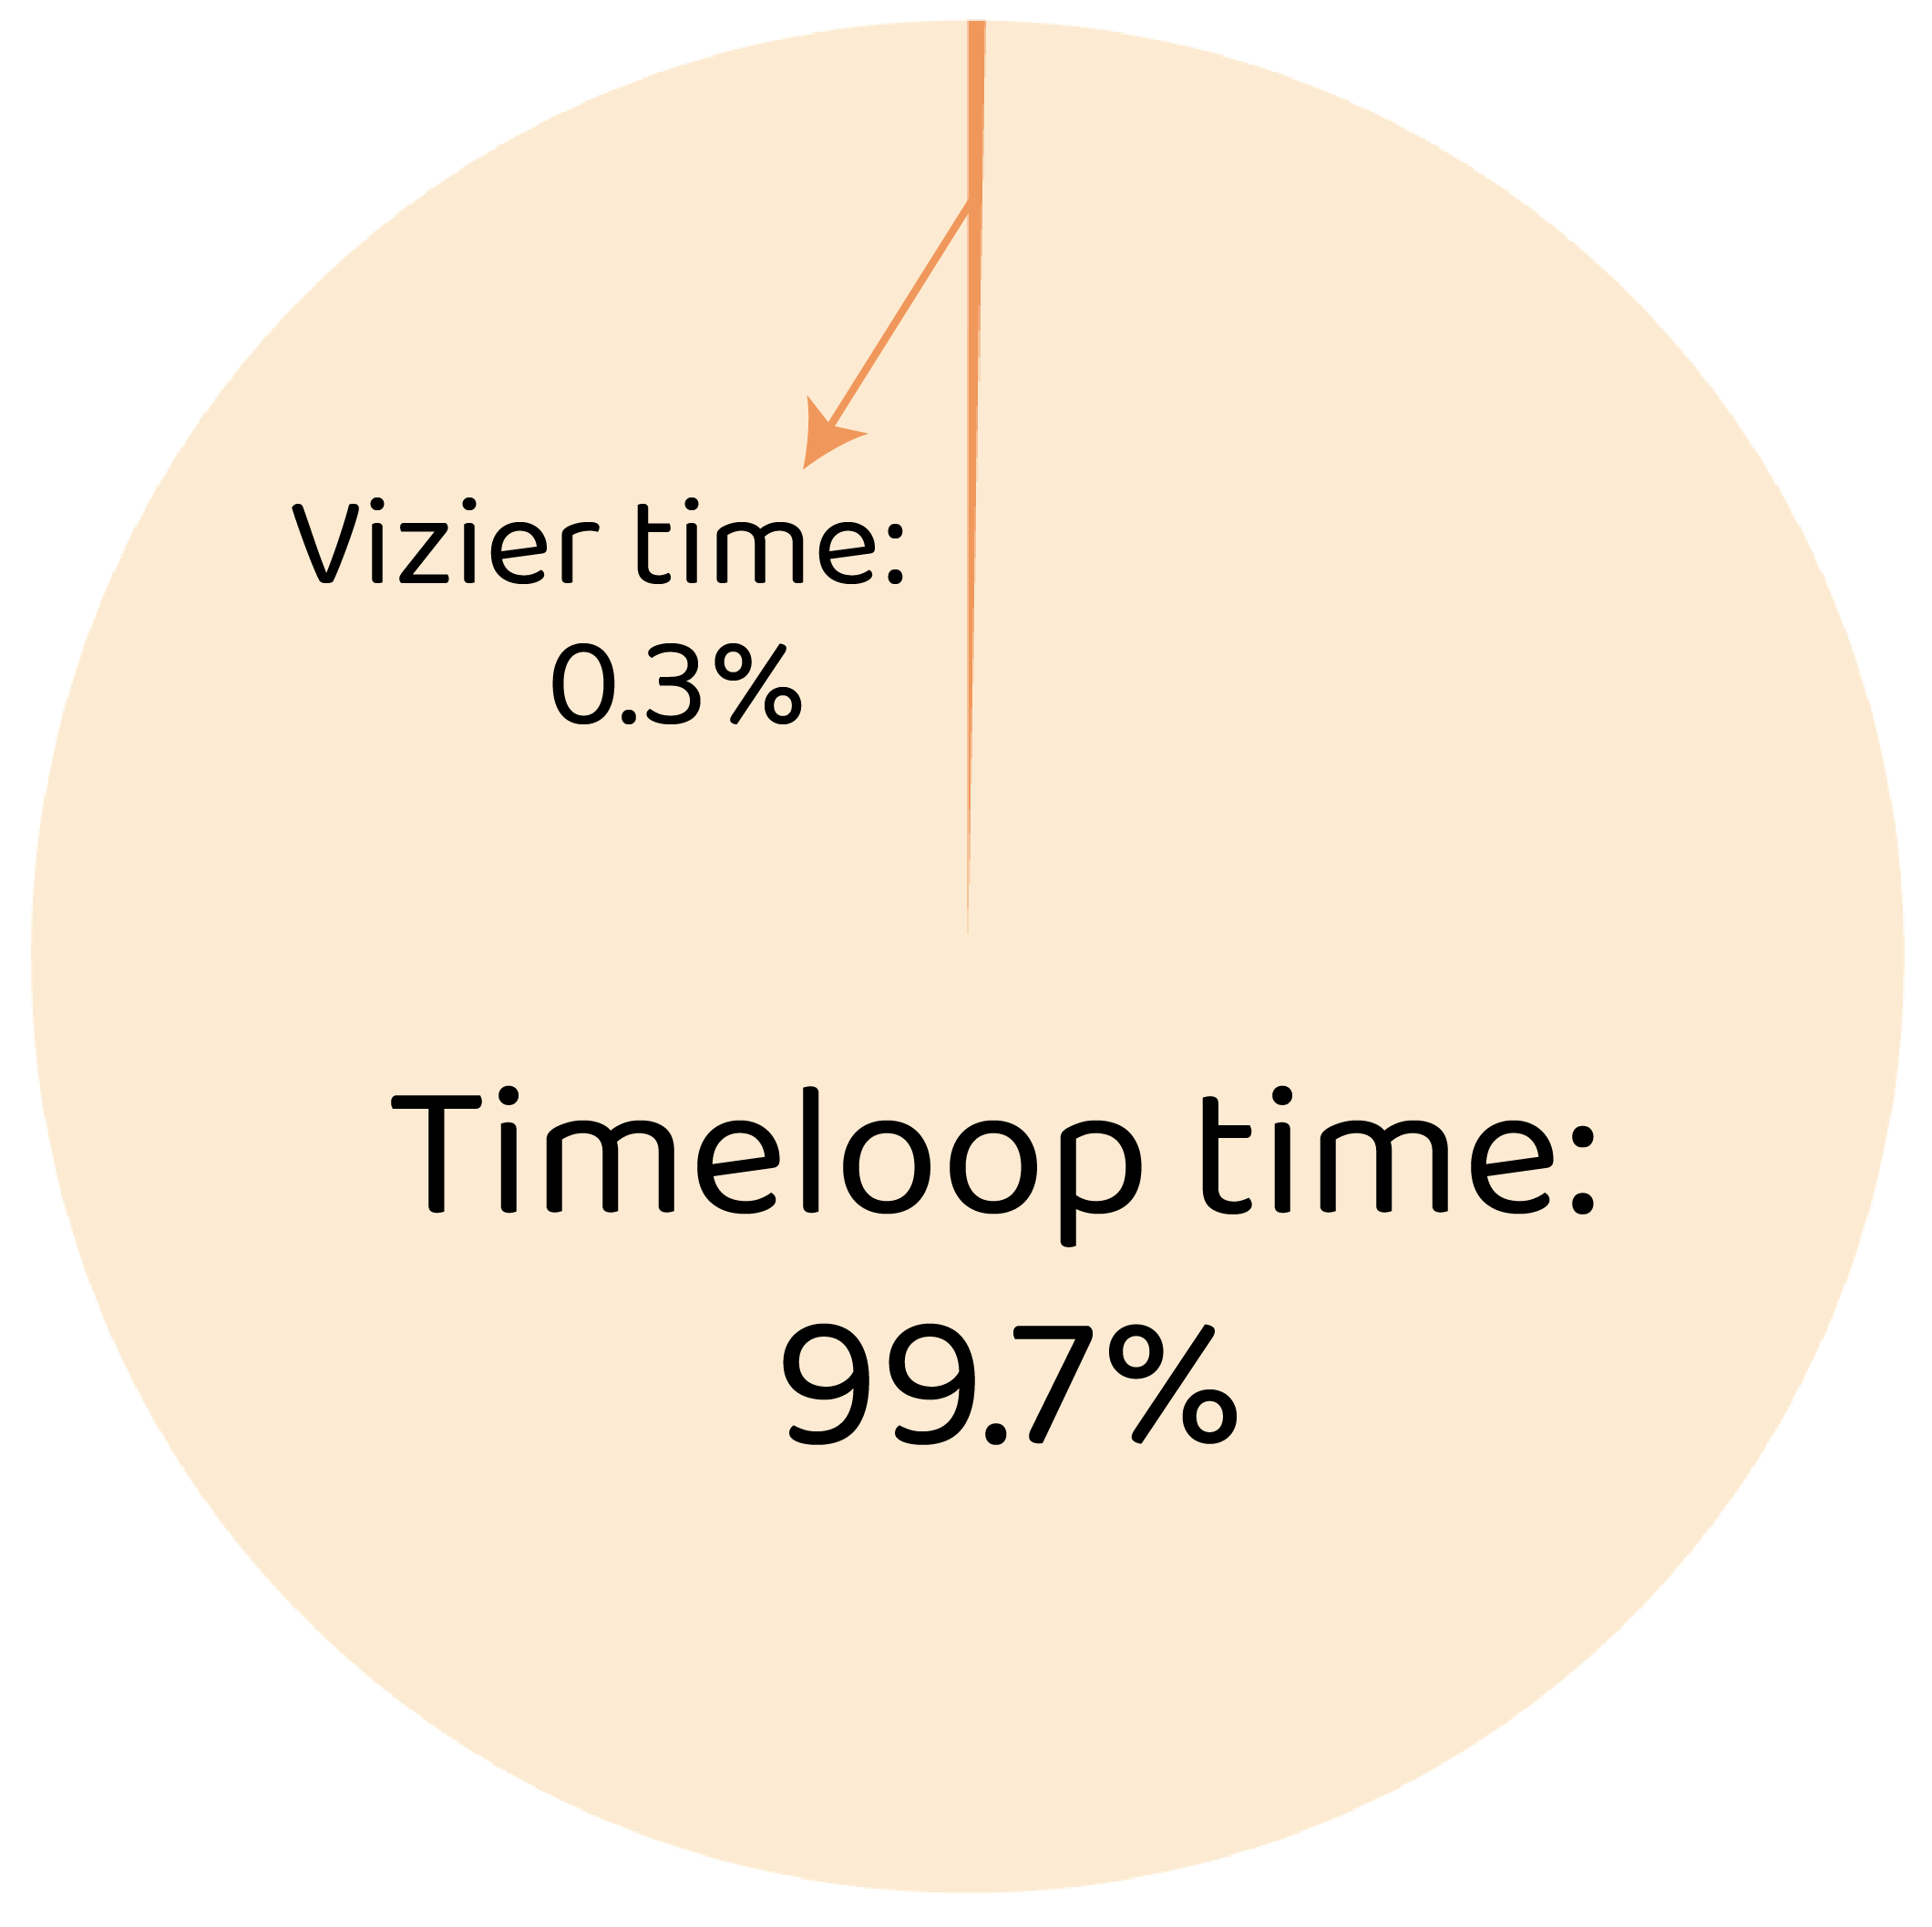
\includegraphics[width=\linewidth]{fig3/timeloop_vs_vizier.png}
% %     \caption{Per-trial wall-clock breakdown.}
% %     \label{fig:timeloop-time}
% %     \vspace{-10pt}
% % \end{wrapfigure}
% % Despite V0's improvements, it inherits the sequential dependence on external tiling tools (e.g., Timeloop) because it lacks a linear expression for non-linear tiling-fusion interactions. As shown in Figure~\ref{fig:timeloop-time}, Timeloop accounts for over 99\% of per-trial latency, creating a prohibitive bottleneck for multi-thousand-trial searches. To resolve this, CHEETAH-V1 internalizes tiling by precomputing Pareto-pruned configurations and encoding them as decision variables. This removes Timeloop from the critical path, collapsing each trial to a single Vizier-proposal and LP-solve step. We start with introducing the preprocessing stage below before presenting the full formulation in Section~\ref{sec::v1}.

% % % The limitations of prior work is still inherited in the V0 formulation due to the difficulty of expressing non-linear relationships as linear constraints. Therefore tiling decisions $(\Tmax_i, \Tmin_i, t_i^k)$ are fixed constants provided by additional software, such as Timeloop. A natural question is whether this sequential dependence also creates a \emph{runtime} bottleneck. Figure~\ref{fig:timeloop-time} confirms that it does: across different models, Timeloop scheduling on average accounts for over 99\% of per-trial wall-clock time, while the Vizier proposal and fusion ILP together consume less than 1\% on average. Because the outer loop requires thousands of trials to converge, the cumulative cost of repeated Timeloop invocations dominates the total search budget. This observation motivates a key design choice in CHEETAH-V1: rather than calling Timeloop online during each trial, we precompute a Pareto-pruned set of tiling configurations once (Section~\ref{sec:pareto}) and encode the tiling selection as decision variables \emph{inside} the LP. This eliminates Timeloop from the per-trial critical path entirely, reducing each trial to a single Vizier-proposal$\,\to\,$LP-solve step.

% % % CHEETAH-V1 captures tiling as a \emph{decision variable} inside the LP, enabling the solver to jointly optimize tiling and fusion. We start with describing our preprocessing stage in Section~\ref{sec:pareto} before presenting the full formulation in Section~\ref{sec::v1}.


% % \paragraph{Pareto Pruning Pre-Pass.} The raw tiling search space for a $7$-dimensional convolution loop with $3$ memory levels is $\mathcal O(10^7)$ configurations per operation. We reduce this to a tractable Pareto-optimal subset $\mathcal{C}_i$ for each operation $i$ via a pre-pass for (1) L1 feasibility where configurations whose tiled working set exceeds L1 scratchpad capacity $C_{L1}$ are discarded; (2) Pareto optimality where a configuration $c$ is retained only if no other configuration achieves both lower $\Tmax_i(c)$ \emph{and} smaller working-set size in the Global Buffer.

% % In practice, Pareto pruning reduces $\mathcal O(10^7)$ raw configurations to $|\mathcal{C}_i| \approx 10^2$ to $10^3$ per operation. Timeloop is run once per (operation, configuration) pair, producing the triple $(\Tmin_i(c), \Tmax_i(c), t_i^k(c))$ for each retained configuration $c \in \mathcal{C}_i$. These are precomputed constants---the LP solver makes no Timeloop calls at solve time.

% % \paragraph{Time-invariant Pareto fronts.}
% % A key observation is that the Pareto front shape is invariant to memory time: configurations are ranked by compute cycles and working-set bytes, neither of which depends on bandwidth. Changing bandwidth rescales the DRAM access cost $t_i^k(c)$ uniformly. This means the Pareto-pruned configuration sets can be precomputed \emph{once} and reused across all Vizier trials that share the same compute configuration class, amortizing the expensive Timeloop precomputation.

% % % \subsubsection{The Joint CHEETAH-V1 LP Formulation}\label{sec::v1}

% % \paragraph{From fixed constants to decision variables.}
% % In static and V0 formulations, Timeloop selects a single tiling per operation externally and passes the results to the LP as fixed constants $\Tmax_i$, $\Tmin_i$, $t_i^k$. The DRAM savings from pinning tensor $k$ of operation $i$ is then simply $t_i^k \cdot p_{i,o(i)}^k$---a constant times a variable, which is already linear. V1 brings this tiling choice \emph{inside} the LP by introducing \textbf{tiling selection variables} $y_{i,c} \in [0,1]$, one per Pareto-optimal configuration $c \in \mathcal{C}_i$ from the pre-pass, with the constraint $\sum_c y_{i,c} = 1$ (exactly one configuration is selected per operation). The Timeloop-precomputed constants $\Tmax_i(c)$, $\Tmin_i(c)$, $t_i^k(c)$ now become \emph{per-configuration coefficients} indexed by $c$. This means the DRAM savings term becomes $t_i^k(c) \cdot y_{i,c} \cdot p_{\text{assoc}(i,k),\, o(i)}$. This is a product of \emph{two} decision variables, which is bilinear and cannot be handled by a convex programming directly.
 
% % % \paragraph{Linearization via McCormick envelopes.}
% % % We linearize this product exactly via the classical McCormick substitution. Specifically,  we introduce \textbf{auxiliary variables} $w_{i,c,k} := y_{i,c} \cdot p_{\text{assoc}(i,k),\, o(i)}$ that represent the joint effect of selecting tiling $c$ \emph{and} pinning tensor $k$, constrained by:
% % % \begin{equation}
% % % \label{eq:mccormick}
% % % \begin{aligned}
% % %     w_{i,c,k} &\leq y_{i,c}, \qquad
% % %     w_{i,c,k} \leq p_{\text{assoc}(i,k),\, o(i)} \\
% % %     w_{i,c,k} &\geq y_{i,c} + p_{\text{assoc}(i,k),\, o(i)} - 1, \qquad
% % %     w_{i,c,k} \geq 0
% % % \end{aligned}
% % % \end{equation}
% % % Since both factors lie in $[0,1]$, these four constraints force $w_{i,c,k} = y_{i,c} \cdot p$ at any integer vertex, requiring no manually tuned constants. Together, $y_{i,c}$ and $w_{i,c,k}$ account for 1.6M of the 2.08M variables in the \Vone~ LP (Table~\ref{tab:v1_scale}). \todo{change to MoE?}

% % \paragraph{Linearization via McCormick envelopes.}
% % We linearize this product exactly via the classical McCormick substitution \citep{mccormick1976computability}. Specifically, we introduce \textbf{auxiliary variables} $w_{i,c,k} := y_{i,c} \cdot p_{\text{assoc}(i,k),\, o(i)}$ that represent the joint effect of selecting tiling $c$ \emph{and} pinning tensor $k$, constrained by:
% % \begin{equation}
% % \label{eq:mccormick}
% % \begin{aligned}
% %     w_{i,c,k} &\leq y_{i,c}, \qquad
% %     w_{i,c,k} \leq p_{\text{assoc}(i,k),\, o(i)} \\
% %     w_{i,c,k} &\geq y_{i,c} + p_{\text{assoc}(i,k),\, o(i)} - 1, \qquad
% %     w_{i,c,k} \geq 0
% % \end{aligned}
% % \end{equation}
% % Since both factors lie in $[0,1]$, these four constraints force $w_{i,c,k} = y_{i,c} \cdot p$ at any integer vertex, requiring no manually tuned constants. Together, $y_{i,c}$ and $w_{i,c,k}$ constitute the majority of V1's decision variables (Table~\ref{tab:v1_scale}).

% % \paragraph{The Joint CHEETAH-V1 LP Formulation.}
% % Combining tiling selection, time-indexed placement, rematerialization, and McCormick linearization, the full V1 formulation is:
% % \begin{equation}
% % \begin{aligned}
% % \min \quad & \sum_{i \in \mathcal{N}} T_i + \sum_{i \in \mathcal{N}} \sum_{t \in \mathcal{T}} c_i^{\text{remat}} \, r_{i,t} \\[4pt]
% % \text{s.t.} \quad
% % & \sum_{c \in \mathcal{C}_i} y_{i,c} = 1 & \forall\, i \in \mathcal{N} \\[3pt]
% % & T_i \geq \max\!\left(\sum_{c \in \mathcal{C}_i} \Tmin_i(c)\, y_{i,c},\;\; \sum_{c \in \mathcal{C}_i} \Tmax_i(c)\, y_{i,c} - \sum_{c \in \mathcal{C}_i} \sum_{k} t_i^k(c)\, w_{i,c,k}\right) & \forall\, i \in \mathcal{N} \\[3pt]
% % & w_{i,c,k} \leq y_{i,c}, \quad w_{i,c,k} \leq p_{\text{assoc}(i,k),\, o(i)}, \quad w_{i,c,k} \geq y_{i,c} + p_{\text{assoc}(i,k),\, o(i)} - 1 & \forall\, i, c, k \\[3pt]
% % & \sum_{e \in \mathcal{E}} d_e\, p_{e,t} + \sum_{i \in \mathcal{N}} d_i^W\, p_{i,t}^W \leq \CGM & \forall\, t \in \mathcal{T} \\[3pt]
% % & p_{e,t} \leq p_{e,t-1} + r_{\text{src}(e),\, t} & \forall\, e,\, t > o(\text{src}(e)) \\
% % & p_{i,t}^W \leq p_{i,t-1}^W & \forall\, i,\, t > o(i) \\[3pt]
% % & r_{i,t} = 0 \;\; \forall\, t \leq o(i); \quad r_{i,t} \leq \min\!\big(p_{e,t},\, p_{i,t}^W\big) \;\; \forall\, e \in \text{in}(i),\, t > o(i) \\[3pt]
% % & T_i,\, p_{e,t},\, p_{i,t}^W,\, r_{i,t},\, w_{i,c,k} \geq 0 &
% % \end{aligned}
% % \tag{V1}\label{eq:v1}
% % \end{equation}

% % \paragraph{Variable and constraint digest.}
% % The V1 formulation inherits all the features of the V0 formulation, and additionally captures tiling by introducing selection variables
% % $y_{i,c} \in [0,1]$, constrained by $\sum_c y_{i,c} = 1$, to choose
% % from $|\mathcal{C}_i|$ Pareto-optimal configurations.
% % Each configuration defines compute costs $T_i^{\max}(c)$,
% % $T_i^{\min}(c)$, and per-tensor DRAM savings $t_i^k(c)$.
% % We linearize the resulting bilinear DRAM-savings term exactly via
% % McCormick auxiliary variables $w_{i,c,k}$, which enforce $w_{i,c,k} \;=\; y_{i,c} \cdot p_{\mathrm{assoc}(i,k),\,o(i)}$ at integer vertices without a relaxation gap.

% % Per-operation latency $T_i$ is lower-bounded by the weighted
% % configuration floor $\sum_c T_i^{\min}(c)\, y_{i,c}$ and the weighted
% % off-chip cost $\sum_c T_i^{\max}(c)\, y_{i,c}$ minus achievable savings
% % $\sum_{c,k} t_i^k(c)\, w_{i,c,k}$.
% % This coupling enables the solver to accept sub-optimal local tiling
% % (higher $T_i^{\max}$) if its smaller memory footprint unlocks global
% % fusion gains that outweigh the compute-utilization loss.
% % Capacity and persistence constraints carry over from V0, utilizing
% % edge-indexed placement $p_{e,t}$ to handle multi-fanout nodes.
% % For DeepSeek-V3, the V1 LP scales to approximately 2.5M variables,
% % 3.0M constraints and 6.1M nonzeros. Table~\ref{tab:v1_scale} provides a representative breakdown, Table~\ref{tab:comparison} summarizes features of each formulation; full per-model sizes are in Table~\ref{tab:exp1_lp_sizes} and \ref{tab:exp2_cluster_lp_sizes}. 



% % % The V1 formulation extends V0 by making the tiling configuration a decision variable. The selection variables $y_{i,c} \in [0,1]$, with $\sum_c y_{i,c} = 1$, choose among $|\mathcal{C}_i|$ Pareto-optimal tiling configurations precomputed by Timeloop (Section~\ref{sec:pareto}). Each configuration $c$ determines the operation's compute cost $T_i^{\max}(c)$, on-chip floor $T_i^{\min}(c)$, and per-tensor DRAM savings $t_i^k(c)$.
% % % The DRAM savings term $t_i^k(c) \cdot y_{i,c} \cdot p_{\text{assoc}(i,k),\,o(i)}$ 
% % % is bilinear in the tiling selection and placement variables; we linearize it 
% % % via McCormick auxiliary variables $w_{i,c,k}$, constrained by 
% % % $w_{i,c,k} \leq y_{i,c}$, $w_{i,c,k} \leq p_{\text{assoc}(i,k),\,o(i)}$, and 
% % % $w_{i,c,k} \geq y_{i,c} + p_{\text{assoc}(i,k),\,o(i)} - 1$. 
% % % These three inequalities force $w_{i,c,k} = y_{i,c} \cdot p_{\text{assoc}(i,k),\,o(i)}$ 
% % % at any integer-feasible point (\cref{prop:mccormick_exact}), so the LP exactly captures the 
% % % bilinear interaction without introducing any relaxation gap at integer vertices.
% % % The $T_i$ lower bound now takes the maximum of two configuration-dependent terms: the weighted on-chip floor $\sum_c T_i^{\min}(c)\, y_{i,c}$ and the weighted off-chip cost minus achievable savings $\sum_c T_i^{\max}(c)\, y_{i,c} - \sum_{c,k} t_i^k(c)\, w_{i,c,k}$.
% % % This coupling is the core novelty of V1: the solver can accept a tiling with higher $T_i^{\max}(c)$ (lower compute utilization) if its smaller working set enables pinning decisions that reduce total DRAM traffic by more than the utilization loss.
% % % All remaining constraints---memory capacity, persistence, and rematerialization---carry over from V0 with edge-indexed placement variables $p_{e,t}$ replacing per-tensor $p_{i,t}^k$ to correctly handle skip connections and multi-fanout nodes. For our largest workload, DeepSeek-V3 ($L \approx 6{,}300$ operations), the V1 LP contains approximately 2.5M variables, 3.0M constraints, and 6.1M nonzeros. Table~\ref{tab:v1_scale} provides a representative breakdown; full per-model sizes are in Table~\ref{tab:v1_scale}. 
% % % \paragraph{Key constraint interactions.}
% % % The execution-time constraints (lines 2--3: the upper and lower bounds for $T_i$) capture the central trade-off that is unique to \Vone: the LP must commit to a tiling configuration $c$ (via $y_{i,c}$) that sets both the baseline compute cost $\Tmax_i(c)$ and the achievable DRAM savings $t_i^k(c)$. A configuration with smaller tiles may have higher $\Tmax_i(c)$ (lower compute utilization) but smaller working sets, enabling more aggressive pinning. The LP balances these trade-offs simultaneously---precisely the cross-stage interaction that the sequential pipeline cannot discover.
 
% % % The edge-indexed persistence constraint (line 8: $p_{e,t} \leq p_{e,t-1} + r_{\text{src}(e),\, t}$) and the memory capacity constraint (line 7: lower bound on $\CGM$) are inherited from \Vzero, which introduced per-edge placement variables $p_{e,t}$ to correctly model skip connections. \Vone~ extends this by coupling edge sizes to the tiling selection---since different configurations $c$ produce different activation working sets, the LP can now jointly reason about how tiling choices affect memory pressure across skip connections.


% % \begin{figure}[ht!]
% % \begin{minipage}[t]{0.48\textwidth}
% % \vspace{0pt}
% % \centering
% % \captionof{table}{V1 variable and constraint counts
% % (representative, DeepSeek-V3).}
% % \label{tab:v1_scale}
% % \footnotesize
% % \begin{tabular}{@{}ll@{}}
% % \toprule
% % \textbf{Variable} & \textbf{Role} \\
% % \midrule
% % $T_i$       & Per-operation execution time \\
% % $y_{i,c}$   & Tiling config selection ($|\mathcal{C}_i|$ options) \\
% % $p_{e,t}$   & Edge-indexed activation placement \\
% % $p_{i,t}^W$ & Weight placement \\
% % $r_{i,t}$   & Rematerialization indicator \\
% % $w_{i,c,k}$ & McCormick auxiliaries ($y_{i,c} \cdot p$) \\
% % % \midrule
% % % \multicolumn{2}{@{}l}{\textbf{DeepSeek-V3 totals}
% % %                        ($L \approx 6{,}300$)} \\
% % % \midrule
% % % Variables   & $2{,}504{,}019$ \\
% % % Constraints & $2{,}983{,}450$ \\
% % % Nonzeros    & $6{,}094{,}156$ \\
% % \bottomrule
% % \end{tabular}
% % \end{minipage}%
% % \hspace{0.02\textwidth}%
% % \begin{minipage}[t]{0.48\textwidth}
% % \vspace{0pt}
% % \centering
% % \captionof{table}{Comparison of static, V0, and V1 formulations.}
% % \label{tab:comparison}
% % \footnotesize
% % \begin{tabular}{@{}lccc@{}}
% % \toprule
% % \textbf{Property} & \textbf{Static} & \textbf{V0} & \textbf{V1} \\
% % \midrule
% % Joint tiling + fusion    & $\times$ & $\times$   & \checkmark \\
% % Time-indexed placement   & $\times$ & \checkmark & \checkmark \\
% % Rematerialization        & $\times$ & \checkmark & \checkmark \\
% % Relaxed skip connections & $\times$ & Partial    & \checkmark \\
% % \bottomrule
% % \end{tabular}

% % \medskip
% % \raggedright
% % \footnotesize
% % % \textbf{Comparison across formulations.}
% % % Table~\ref{tab:comparison} summarizes the progression from the
% % % static formulation through V0 to V1.
% % \end{minipage}
% % \end{figure}


% % % \begin{table}[ht!]
% % % \centering
% % % \caption{V1 variable and constraint counts (representative, DeepSeek-V3).}
% % % \label{tab:v1_scale}
% % % \small
% % % \begin{tabular}{lrl}
% % % \toprule
% % % \textbf{Variable} & \textbf{Role} \\
% % % \midrule
% % % $T_i$ & Per-operation execution time \\
% % % $y_{i,c}$ & Tiling configuration selection ($|\mathcal{C}_i|$ options per op) \\
% % % $p_{e,t}$ & Edge-indexed activation placement \\
% % % $p_{i,t}^W$ & Weight placement \\
% % % $r_{i,t}$ & Rematerialization indicator \\
% % % $w_{i,c,k}$ & McCormick auxiliaries ($y_{i,c} \cdot p$) \\
% % % \midrule
% % % \multicolumn{2}{l}{\textbf{DeepSeek-V3 totals} ($L \approx 6{,}300$)} \\
% % % \midrule
% % % Variables & 2,504,019 \\
% % % Constraints & 2,983,450 \\
% % % Nonzeros & 6,094,156 \\
% % % \bottomrule
% % % \end{tabular}
% % % \end{table}
% % % \paragraph{Comparison across formulations.}
% % % Table~\ref{tab:comparison} summarizes the progression from static through V0 to V1.
% % % \begin{table}[ht!]
% % % \centering
% % % \caption{Comparison of static, V0, and V1 formulations.}
% % % \label{tab:comparison}
% % % \small
% % % \begin{tabular}{lccc}
% % % \toprule
% % % \textbf{Property} & \textbf{static} & \textbf{V0} & \textbf{V1} \\
% % % \midrule
% % % Joint tiling + fusion & \texttimes & \texttimes & \checkmark \\
% % % Time-indexed placement & \texttimes & \checkmark & \checkmark \\
% % % Rematerialization & \texttimes & \checkmark & \checkmark \\
% % % Relaxed skip connections & \texttimes & Partial & \checkmark \\
% % % % Config-dependent DRAM savings & \texttimes & \texttimes & \checkmark \\ 
% % % % Bilinear linearization & --- & --- & McCormick \\
% % % \bottomrule
% % % \end{tabular}
% % % \end{table}

% % % \paragraph{Structural invariance for efficient LLM integration.}
% % % A practical advantage of both our LP formulations is that the constraint matrix sparsity pattern is invariant across hardware configurations---only the numerical coefficients change. This means:
% % % \begin{itemize}
% % %     \item The LP solver's preconditioner can be designed once per neural network model and reused across all Vizier trials.
% % %     \item An LLM-Architect can reason about constraint structure (which constraints are binding, which variables are fractional) without needing to understand the full LP.
% % %     \item Warm-starting from a previous trial's LP solution is straightforward since the variable indexing is stable.
% % % \end{itemize}

% % \subsection{Strategic Intelligence: LLM-Guided Outer Search}
% % \label{sec:llm_outer}
% % We use Google Vizier as a black-box Bayesian optimizer to propose hardware configurations. While effective, vanilla Vizier treats search as pure function optimization, often requiring thousands of iterations to identify suboptimal regions without leveraging structural hardware-workload knowledge. To address this, we introduce an LLM-guided outer-loop controller based on SkyDiscovery that reasons about co-design decisions. This integration is enabled by the CHEETAH-V1 formulation, which removes the Timeloop bottleneck to reduce trial times from days to hours.

% % In this hybrid loop, the LLM acts as a \emph{Causal Architect}: it reads a compact \emph{Causal Ledger} of past trials---containing hardware parameters, validity, Perf/TDP, LP duals/slacks, MFU, and roofline diagnostics---and emits a \emph{campaign patch} that constrains Vizier's search to a workload-appropriate architectural neighborhood (e.g., adjusting Global Memory floors, DRAM bandwidth ranges, or systolic shapes). A deterministic \emph{Campaign Validator} clips or rejects each patch to enforce physical constraints (TDP caps, area limits, MAC/bandwidth coupling), preventing the LLM from proposing implausible regions. Vizier then performs local Bayesian optimization within the approved patch, and the V1 LP evaluates each concrete candidate. A \emph{Roofline Auditor} rejects any result whose predicted latency falls below the physical lower bound $\mathrm{LB} = \max(t_{\text{compute}}, t_{\text{memory}})$. The ledger records each intervention and outcome, preventing redundant exploration and ensuring full auditability. The online Architect is implemented as Qwen2.5-7B-Instruct with a LoRA adapter trained on past trial logs; a larger teacher model (DeepSeek-V3.2) was used offline for campaign label generation. The full loop details are in Appendix~\ref{app:llm_loop}.


% % page edit

% % \section{Methodology}
% % \label{sec:methods}

% % We present the CHEETAH (\acroletter{C}o-designed \acroletter{H}ardware \acroletter{E}xploration via \acroletter{E}fficient \acroletter{T}hroughput and \acroletter{H}ybrid-search) framework in three parts: Section~\ref{sec:v0} introduces CHEETAH-V0, which extends the static fusion ILP with time-indexed placement and rematerialization. Section~\ref{sec:v1} presents CHEETAH-V1, which jointly optimizes tiling and fusion via McCormick linearization. Section~\ref{sec:llm_outer} describes the LLM-Architect outer loop.


% % % \subsection{\Vzero~: Multi-Period Placement with Rematerialization}
% % \subsection{CHEETAH-V0: Multi-Period Placement with Rematerialization}
% % \label{sec:v0}

% % Our first extension models the neural network's execution as a sequence of $T$ discrete timesteps (one per operation in execution order). This decides at which time, which tensor is pinned, evicted, or recomputed to optimally minimize cycle counts. The key features are:

% % \paragraph{Time-indexed placement.}
% % Instead of a single binary $p_i^k$ per tensor, we introduce $p_{i,t}^k \in [0,1]$ for each tensor $k$ of layer $i$ at each timestep $t$. A tensor can be pinned at timestep $t=5$, and evicted at $t=10$. This models a dynamic memory manager within a single inference pass.

% % \paragraph{Rematerialization.}
% % Rather than always paying DRAM bandwidth to reload an evicted tensor, we introduce variables $r_{i,t} \in [0,1]$ indicating that layer $i$ is recomputed at timestep $t$ to restore its output to the Global Buffer. This is particularly valuable for models such as EfficientNet, where depthwise convolutions account for only ${\sim}5\%$ of total FLOPs but produce large activation tensors. Recomputing a depthwise layer to avoid re-reading 6\,MiB from DRAM at 256\,GB/s can be faster than the DRAM reload itself.

% % \paragraph{Relaxed skip-connection handling.}
% % We lift the limitation of our baseline original ILP, which restricts activation pinning to consecutively-executed operations and limits multi-fanout nodes so that at most one consumer benefits from on-chip data. CHEETAH-V0 uses edge-indexed placement variables $p_{e,t}$ for each edge $e \in \mathcal{E}$ of the dataflow graph, correctly modeling the case where one consumer of a skip connection benefits from on-chip data while another does not.

% % The CHEETAH-V0 LP formulation is:
% % \begin{equation}
% % % \label{eq:v0}
% % \begin{aligned}
% % \min \quad & \sum_{i \in \mathcal{N}} T_i + \sum_{i \in \mathcal{N}} \sum_{t \in \mathcal{T}} c_i^{\text{remat}} \, r_{i,t} \\
% % \text{s.t.} \quad
% % & T_i \geq \Tmax_i - \sum_{k \in \{I,O,W\}} t_i^k \cdot p_{i,o(i)}^k & \forall\, i \in \mathcal{N} \\
% % & T_i \geq \Tmin_i & \forall\, i \in \mathcal{N} \\
% % & \sum_{i \in \mathcal{N}} \sum_{k} d_i^k \, p_{i,t}^k \leq \CGM & \forall\, t \in \mathcal{T} \\
% % & p_{i,t}^k \leq p_{i,t-1}^k + r_{i,t} & \forall\, i, t, k \in \{I,O\} \\
% % & p_{i,t}^W \leq p_{i,t-1}^W & \forall\, i, t \\
% % & r_{i,t} = 0 & \forall\, i, t \leq o(i) \\
% % & 0 \leq p_{i,t}^k, r_{i,t} \leq 1 &
% % \end{aligned}
% % \tag{V0}\label{eq:v0}
% % \end{equation}


% % where $o(i)$ is the execution order of operation $i$, $d_i^k$ is the byte size of tensor $k$ for layer $i$, and $c_i^{\text{remat}}$ is the recomputation cost.

% % \paragraph{Variable and constraint digest.}
% % The V0 objective minimizes the sum of execution times $\sum_i T_i$ and
% % rematerialization costs $c_i^{\text{remat}}\, r_{i,t}$.
% % Per-operation latency $T_i$ is lower-bounded by the physical on-chip
% % floor $T_i^{\min}$ and the off-chip time $T_i^{\max}$ adjusted for DRAM
% % savings $t_i^k \cdot p_{i,o(i)}^k$ from pinned tensors.
% % Placement variables $p_{i,t}^k \in [0,1]$ track Global Memory residency
% % for inputs, outputs, and weights at each timestep, subject to a global
% % capacity constraint $C_{\text{GM}}$. Persistence is governed by $p_{i,t}^k \;\leq\; p_{i,t-1}^k + r_{i,t},$ enforcing that activations are either resident from the previous timestep
% % or recomputed; weight tensors satisfy the stricter monotone constraint
% % $p_{i,t}^W \leq p_{i,t-1}^W$, as weights cannot be rematerialized.
% % Rematerialization $r_{i,t}$ is only permitted post-execution
% % ($t > o(i)$) and requires on-chip availability of both inputs and
% % weights.
% % For DeepSeek-V3 ($L \approx 6{,}300$), this formulation yields a
% % large-scale program with approximately 3.3M variables and 3.7M
% % constraints.


% % % \subsection{\textcolor{skyblue}{V1}: Joint Tiling and Fusion via McCormick Linearization}
% % \subsection{CHEETAH-V1: Joint Tiling and Fusion via McCormick Linearization}
% % \label{sec:v1}

% % \begin{wrapfigure}{r}{0.2\linewidth}
% %     \vspace{-12pt}
% %     \centering
% %     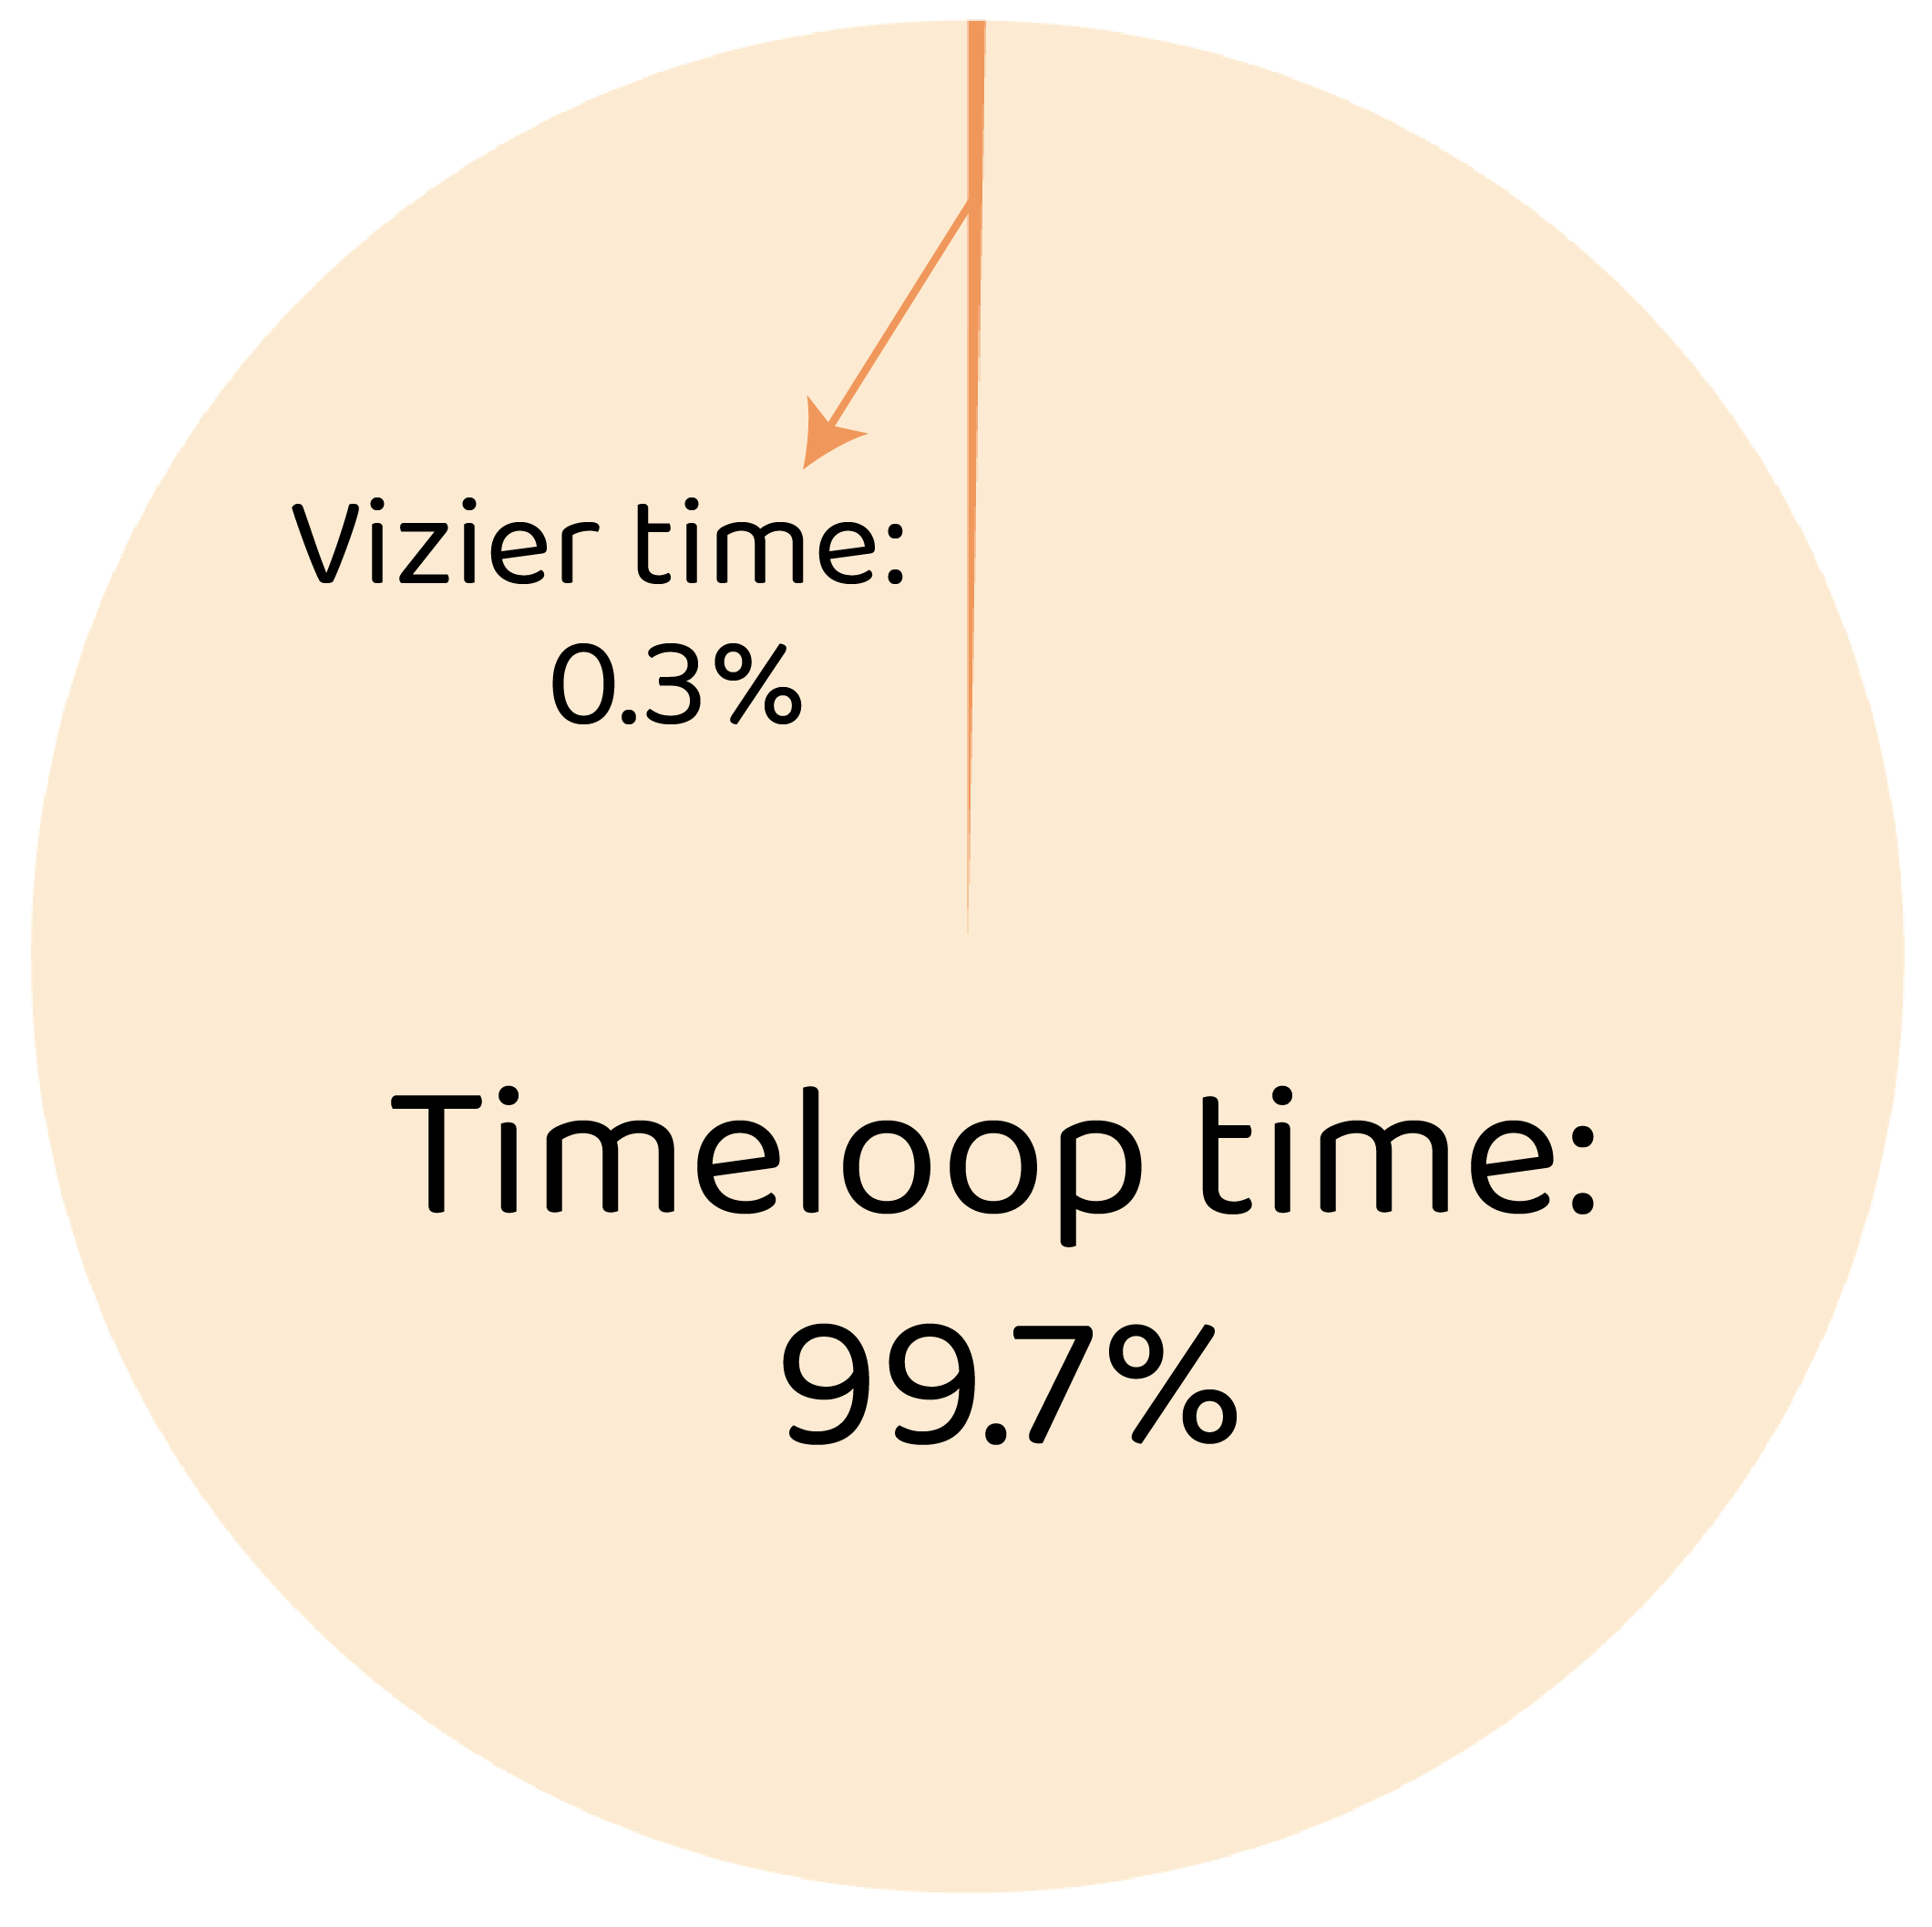
\includegraphics[width=\linewidth]{fig3/timeloop_vs_vizier.png}
% %     \caption{Per-trial wall-clock breakdown.}
% %     \label{fig:timeloop-time}
% %     \vspace{-10pt}
% % \end{wrapfigure}
% % Despite V0's improvements, it inherits the sequential dependence on external tiling tools (e.g., Timeloop) because it lacks a linear expression for non-linear tiling-fusion interactions. As shown in Figure~\ref{fig:timeloop-time}, Timeloop accounts for over 99\% of per-trial latency, creating a prohibitive bottleneck for multi-thousand-trial searches. To resolve this, CHEETAH-V1 internalizes tiling by precomputing Pareto-pruned configurations and encoding them as decision variables. This removes Timeloop from the critical path, collapsing each trial to a single Vizier-proposal and LP-solve step. We start with introducing the preprocessing stage below before presenting the full formulation in Section~\ref{sec::v1}.

% % % The limitations of prior work is still inherited in the V0 formulation due to the difficulty of expressing non-linear relationships as linear constraints. Therefore tiling decisions $(\Tmax_i, \Tmin_i, t_i^k)$ are fixed constants provided by additional software, such as Timeloop. A natural question is whether this sequential dependence also creates a \emph{runtime} bottleneck. Figure~\ref{fig:timeloop-time} confirms that it does: across different models, Timeloop scheduling on average accounts for over 99\% of per-trial wall-clock time, while the Vizier proposal and fusion ILP together consume less than 1\% on average. Because the outer loop requires thousands of trials to converge, the cumulative cost of repeated Timeloop invocations dominates the total search budget. This observation motivates a key design choice in CHEETAH-V1: rather than calling Timeloop online during each trial, we precompute a Pareto-pruned set of tiling configurations once (Section~\ref{sec:pareto}) and encode the tiling selection as decision variables \emph{inside} the LP. This eliminates Timeloop from the per-trial critical path entirely, reducing each trial to a single Vizier-proposal$\,\to\,$LP-solve step.

% % % CHEETAH-V1 captures tiling as a \emph{decision variable} inside the LP, enabling the solver to jointly optimize tiling and fusion. We start with describing our preprocessing stage in Section~\ref{sec:pareto} before presenting the full formulation in Section~\ref{sec::v1}.


% % \paragraph{Pareto Pruning Pre-Pass} The raw tiling search space for a $7$-dimensional convolution loop with $3$ memory levels is $\mathcal O(10^7)$ configurations per operation. We reduce this to a tractable Pareto-optimal subset $\mathcal{C}_i$ for each operation $i$ via a pre-pass for (1) L1 feasibility where configurations whose tiled working set exceeds L1 scratchpad capacity $C_{L1}$ are discarded; (2) Pareto optimality where a configuration $c$ is retained only if no other configuration achieves both lower $\Tmax_i(c)$ \emph{and} smaller working-set size in the Global Buffer.

% % In practice, Pareto pruning reduces $\mathcal O(10^7)$ raw configurations to $|\mathcal{C}_i| \approx 10^2$ to $10^3$ per operation. Timeloop is run once per (operation, configuration) pair, producing the triple $(\Tmin_i(c), \Tmax_i(c), t_i^k(c))$ for each retained configuration $c \in \mathcal{C}_i$. These are precomputed constants---the LP solver makes no Timeloop calls at solve time.

% % \paragraph{Time-invariant Pareto fronts.}
% % A key observation is that the Pareto front shape is invariant to memory time: configurations are ranked by compute cycles and working-set bytes, neither of which depends on bandwidth. Changing bandwidth rescales the DRAM access cost $t_i^k(c)$ uniformly. This means the Pareto-pruned configuration sets can be precomputed \emph{once} and reused across all Vizier trials that share the same compute configuration class, amortizing the expensive Timeloop precomputation.

% % \subsubsection{The Joint CHEETAH-V1 LP Formulation}\label{sec::v1}

% % \paragraph{From fixed constants to decision variables.}
% % In static and V0 formulations, Timeloop selects a single tiling per operation externally and passes the results to the LP as fixed constants $\Tmax_i$, $\Tmin_i$, $t_i^k$. The DRAM savings from pinning tensor $k$ of operation $i$ is then simply $t_i^k \cdot p_{i,o(i)}^k$---a constant times a variable, which is already linear. V1 brings this tiling choice \emph{inside} the LP by introducing \textbf{tiling selection variables} $y_{i,c} \in [0,1]$, one per Pareto-optimal configuration $c \in \mathcal{C}_i$ from the pre-pass, with the constraint $\sum_c y_{i,c} = 1$ (exactly one configuration is selected per operation). The Timeloop-precomputed constants $\Tmax_i(c)$, $\Tmin_i(c)$, $t_i^k(c)$ now become \emph{per-configuration coefficients} indexed by $c$. This means the DRAM savings term becomes $t_i^k(c) \cdot y_{i,c} \cdot p_{\text{assoc}(i,k),\, o(i)}$. This is a product of \emph{two} decision variables, which is bilinear and cannot be handled by a convex programming directly.
 
% % % \paragraph{Linearization via McCormick envelopes.}
% % % We linearize this product exactly via the classical McCormick substitution. Specifically,  we introduce \textbf{auxiliary variables} $w_{i,c,k} := y_{i,c} \cdot p_{\text{assoc}(i,k),\, o(i)}$ that represent the joint effect of selecting tiling $c$ \emph{and} pinning tensor $k$, constrained by:
% % % \begin{equation}
% % % \label{eq:mccormick}
% % % \begin{aligned}
% % %     w_{i,c,k} &\leq y_{i,c}, \qquad
% % %     w_{i,c,k} \leq p_{\text{assoc}(i,k),\, o(i)} \\
% % %     w_{i,c,k} &\geq y_{i,c} + p_{\text{assoc}(i,k),\, o(i)} - 1, \qquad
% % %     w_{i,c,k} \geq 0
% % % \end{aligned}
% % % \end{equation}
% % % Since both factors lie in $[0,1]$, these four constraints force $w_{i,c,k} = y_{i,c} \cdot p$ at any integer vertex, requiring no manually tuned constants. Together, $y_{i,c}$ and $w_{i,c,k}$ account for 1.6M of the 2.08M variables in the \Vone~ LP (Table~\ref{tab:v1_scale}). \todo{change to MoE?}

% % \paragraph{Linearization via McCormick envelopes.}
% % We linearize this product exactly via the classical McCormick substitution \citep{mccormick1976computability}. Specifically, we introduce \textbf{auxiliary variables} $w_{i,c,k} := y_{i,c} \cdot p_{\text{assoc}(i,k),\, o(i)}$ that represent the joint effect of selecting tiling $c$ \emph{and} pinning tensor $k$, constrained by:
% % \begin{equation}
% % \label{eq:mccormick}
% % \begin{aligned}
% %     w_{i,c,k} &\leq y_{i,c}, \qquad
% %     w_{i,c,k} \leq p_{\text{assoc}(i,k),\, o(i)} \\
% %     w_{i,c,k} &\geq y_{i,c} + p_{\text{assoc}(i,k),\, o(i)} - 1, \qquad
% %     w_{i,c,k} \geq 0
% % \end{aligned}
% % \end{equation}
% % Since both factors lie in $[0,1]$, these four constraints force $w_{i,c,k} = y_{i,c} \cdot p$ at any integer vertex, requiring no manually tuned constants. Together, $y_{i,c}$ and $w_{i,c,k}$ constitute the majority of V1's decision variables (Table~\ref{tab:v1_scale}).
 

% % % \paragraph{Full formulation.}
% % % Combining tiling selection, time-indexed placement, rematerialization, and McCormick linearization, the full V1  formulation is:

% % % \begin{equation}
% % % % \label{eq:v1}
% % % \begin{aligned}
% % % \min \quad & \sum_{i \in \mathcal{N}} T_i + \sum_{i \in \mathcal{N}} \sum_{t \in \mathcal{T}} c_i^{\text{remat}} \, r_{i,t} \\[4pt]
% % % \text{s.t.} \quad
% % % & \sum_{c \in \mathcal{C}_i} y_{i,c} = 1 & \forall\, i \in \mathcal{N} \\[3pt]
% % % & T_i \geq \sum_{c \in \mathcal{C}_i} \Tmax_i(c)\, y_{i,c} - \sum_{c \in \mathcal{C}_i} \sum_{k} t_i^k(c)\, w_{i,c,k} & \forall\, i \in \mathcal{N} \\[3pt]
% % % & T_i \geq \sum_{c \in \mathcal{C}_i} \Tmin_i(c)\, y_{i,c} & \forall\, i \in \mathcal{N} \\[3pt]
% % % & w_{i,c,k} \leq y_{i,c} & \forall\, i, c, k \\
% % % & w_{i,c,k} \leq p_{\text{assoc}(i,k),\, o(i)} & \forall\, i, c, k \\
% % % & w_{i,c,k} \geq y_{i,c} + p_{\text{assoc}(i,k),\, o(i)} - 1 & \forall\, i, c, k \\[3pt]
% % % & \sum_{e \in \mathcal{E}} d_e\, p_{e,t} + \sum_{i \in \mathcal{N}} d_i^W\, p_{i,t}^W \leq \CGM & \forall\, t \in \mathcal{T} \\[3pt]
% % % & p_{e,t} \leq p_{e,t-1} + r_{\text{src}(e),\, t} & \forall\, e, t > o(\text{src}(e)) \\
% % % & p_{i,t}^W \leq p_{i,t-1}^W & \forall\, i, t > o(i) \\[3pt]
% % % & r_{i,t} = 0 & \forall\, i, t \leq o(i) \\
% % % & r_{i,t} \leq p_{e,t} & \forall\, e \in \text{in}(i), t > o(i) \\
% % % & r_{i,t} \leq p_{i,t}^W & \forall\, i, t > o(i) \\[3pt]
% % % & T_i, p_{e,t}, p_{i,t}^W, r_{i,t}, w_{i,c,k} \geq 0 &
% % % \end{aligned}
% % % \tag{\textcolor{skyblue}{V1}}\label{eq:v1}
% % % \end{equation}
% % % full formulation below in appendix 
% % % \begin{equation}
% % % \begin{aligned}
% % % \min \quad & \sum_{i \in \mathcal{N}} T_i + \sum_{i \in \mathcal{N}} \sum_{t \in \mathcal{T}} c_i^{\text{remat}} \, r_{i,t} \\[4pt]
% % % \text{s.t.} \quad
% % % & \sum_{c \in \mathcal{C}_i} y_{i,c} = 1 & \forall\, i \in \mathcal{N} \\[3pt]
% % % & T_i \geq \max\!\left(\sum_{c \in \mathcal{C}_i} \Tmin_i(c)\, y_{i,c},\;\; \sum_{c \in \mathcal{C}_i} \Tmax_i(c)\, y_{i,c} - \sum_{c \in \mathcal{C}_i} \sum_{k} t_i^k(c)\, w_{i,c,k}\right) & \forall\, i \in \mathcal{N} \\[3pt]
% % % & w_{i,c,k} \leq y_{i,c}, \quad w_{i,c,k} \leq p_{\text{assoc}(i,k),\, o(i)}, \quad w_{i,c,k} \geq y_{i,c} + p_{\text{assoc}(i,k),\, o(i)} - 1 & \forall\, i, c, k \\[3pt]
% % % & \sum_{e \in \mathcal{E}} d_e\, p_{e,t} + \sum_{i \in \mathcal{N}} d_i^W\, p_{i,t}^W \leq \CGM & \forall\, t \in \mathcal{T} \\[3pt]
% % % & p_{e,t} \leq p_{e,t-1} + r_{\text{src}(e),\, t} & \forall\, e,\, t > o(\text{src}(e)) \\
% % % & p_{i,t}^W \leq p_{i,t-1}^W & \forall\, i,\, t > o(i) \\[3pt]
% % % & r_{i,t} = 0 \;\; \forall\, t \leq o(i); \quad r_{i,t} \leq \min\!\big(p_{e,t},\, p_{i,t}^W\big) \;\; \forall\, e \in \text{in}(i),\, t > o(i) \\[3pt]
% % % & T_i,\, p_{e,t},\, p_{i,t}^W,\, r_{i,t},\, w_{i,c,k} \geq 0 &
% % % \end{aligned}
% % % \tag{\textcolor{skyblue}{V1}}\label{eq:v1}
% % % \end{equation}

% % \paragraph{Variable and constraint digest.}
% % The V1 formulation inherits all the features of the V0 formulation, and additionally captures tiling by introducing selection variables
% % $y_{i,c} \in [0,1]$, constrained by $\sum_c y_{i,c} = 1$, to choose
% % from $|\mathcal{C}_i|$ Pareto-optimal configurations.
% % Each configuration defines compute costs $T_i^{\max}(c)$,
% % $T_i^{\min}(c)$, and per-tensor DRAM savings $t_i^k(c)$.
% % We linearize the resulting bilinear DRAM-savings term exactly via
% % McCormick auxiliary variables $w_{i,c,k}$, which enforce $w_{i,c,k} \;=\; y_{i,c} \cdot p_{\mathrm{assoc}(i,k),\,o(i)}$ at integer vertices without a relaxation gap.

% % Per-operation latency $T_i$ is lower-bounded by the weighted
% % configuration floor $\sum_c T_i^{\min}(c)\, y_{i,c}$ and the weighted
% % off-chip cost $\sum_c T_i^{\max}(c)\, y_{i,c}$ minus achievable savings
% % $\sum_{c,k} t_i^k(c)\, w_{i,c,k}$.
% % This coupling enables the solver to accept sub-optimal local tiling
% % (higher $T_i^{\max}$) if its smaller memory footprint unlocks global
% % fusion gains that outweigh the compute-utilization loss.
% % Capacity and persistence constraints carry over from V0, utilizing
% % edge-indexed placement $p_{e,t}$ to handle multi-fanout nodes.
% % For DeepSeek-V3, the V1 LP scales to approximately $2{,}504{,}019$ variables, $2{,}983{,}450$ constraints, and $6{,}094{,}156$ non-zeros. Table~\ref{tab:v1_scale} provides a representative breakdown, Table~\ref{tab:comparison} summarizes features of each more powerful formulation; full per-model sizes are in Table~\ref{tab:exp1_lp_sizes} and \ref{tab:exp2_cluster_lp_sizes}. 



% % % The V1 formulation extends V0 by making the tiling configuration a decision variable. The selection variables $y_{i,c} \in [0,1]$, with $\sum_c y_{i,c} = 1$, choose among $|\mathcal{C}_i|$ Pareto-optimal tiling configurations precomputed by Timeloop (Section~\ref{sec:pareto}). Each configuration $c$ determines the operation's compute cost $T_i^{\max}(c)$, on-chip floor $T_i^{\min}(c)$, and per-tensor DRAM savings $t_i^k(c)$.
% % % The DRAM savings term $t_i^k(c) \cdot y_{i,c} \cdot p_{\text{assoc}(i,k),\,o(i)}$ 
% % % is bilinear in the tiling selection and placement variables; we linearize it 
% % % via McCormick auxiliary variables $w_{i,c,k}$, constrained by 
% % % $w_{i,c,k} \leq y_{i,c}$, $w_{i,c,k} \leq p_{\text{assoc}(i,k),\,o(i)}$, and 
% % % $w_{i,c,k} \geq y_{i,c} + p_{\text{assoc}(i,k),\,o(i)} - 1$. 
% % % These three inequalities force $w_{i,c,k} = y_{i,c} \cdot p_{\text{assoc}(i,k),\,o(i)}$ 
% % % at any integer-feasible point (\cref{prop:mccormick_exact}), so the LP exactly captures the 
% % % bilinear interaction without introducing any relaxation gap at integer vertices.
% % % The $T_i$ lower bound now takes the maximum of two configuration-dependent terms: the weighted on-chip floor $\sum_c T_i^{\min}(c)\, y_{i,c}$ and the weighted off-chip cost minus achievable savings $\sum_c T_i^{\max}(c)\, y_{i,c} - \sum_{c,k} t_i^k(c)\, w_{i,c,k}$.
% % % This coupling is the core novelty of V1: the solver can accept a tiling with higher $T_i^{\max}(c)$ (lower compute utilization) if its smaller working set enables pinning decisions that reduce total DRAM traffic by more than the utilization loss.
% % % All remaining constraints---memory capacity, persistence, and rematerialization---carry over from V0 with edge-indexed placement variables $p_{e,t}$ replacing per-tensor $p_{i,t}^k$ to correctly handle skip connections and multi-fanout nodes. For our largest workload, DeepSeek-V3 ($L \approx 6{,}300$ operations), the V1 LP contains approximately 2.5M variables, 3.0M constraints, and 6.1M nonzeros. Table~\ref{tab:v1_scale} provides a representative breakdown; full per-model sizes are in Table~\ref{tab:v1_scale}. 
% % % \paragraph{Key constraint interactions.}
% % % The execution-time constraints (lines 2--3: the upper and lower bounds for $T_i$) capture the central trade-off that is unique to \Vone: the LP must commit to a tiling configuration $c$ (via $y_{i,c}$) that sets both the baseline compute cost $\Tmax_i(c)$ and the achievable DRAM savings $t_i^k(c)$. A configuration with smaller tiles may have higher $\Tmax_i(c)$ (lower compute utilization) but smaller working sets, enabling more aggressive pinning. The LP balances these trade-offs simultaneously---precisely the cross-stage interaction that the sequential pipeline cannot discover.
 
% % % The edge-indexed persistence constraint (line 8: $p_{e,t} \leq p_{e,t-1} + r_{\text{src}(e),\, t}$) and the memory capacity constraint (line 7: lower bound on $\CGM$) are inherited from \Vzero, which introduced per-edge placement variables $p_{e,t}$ to correctly model skip connections. \Vone~ extends this by coupling edge sizes to the tiling selection---since different configurations $c$ produce different activation working sets, the LP can now jointly reason about how tiling choices affect memory pressure across skip connections.


% % \begin{figure}[ht!]
% % \begin{minipage}[t]{0.48\textwidth}
% % \vspace{0pt}
% % \centering
% % \captionof{table}{V1 variable and constraint counts
% % (representative, DeepSeek-V3).}
% % \label{tab:v1_scale}
% % \footnotesize
% % \begin{tabular}{@{}ll@{}}
% % \toprule
% % \textbf{Variable} & \textbf{Role} \\
% % \midrule
% % $T_i$       & Per-operation execution time \\
% % $y_{i,c}$   & Tiling config selection ($|\mathcal{C}_i|$ options) \\
% % $p_{e,t}$   & Edge-indexed activation placement \\
% % $p_{i,t}^W$ & Weight placement \\
% % $r_{i,t}$   & Rematerialization indicator \\
% % $w_{i,c,k}$ & McCormick auxiliaries ($y_{i,c} \cdot p$) \\
% % % \midrule
% % % \multicolumn{2}{@{}l}{\textbf{DeepSeek-V3 totals}
% % %                        ($L \approx 6{,}300$)} \\
% % % \midrule
% % % Variables   & $2{,}504{,}019$ \\
% % % Constraints & $2{,}983{,}450$ \\
% % % Nonzeros    & $6{,}094{,}156$ \\
% % \bottomrule
% % \end{tabular}
% % \end{minipage}%
% % \hspace{0.02\textwidth}%
% % \begin{minipage}[t]{0.48\textwidth}
% % \vspace{0pt}
% % \centering
% % \captionof{table}{Comparison of static, V0, and V1 formulations.}
% % \label{tab:comparison}
% % \footnotesize
% % \begin{tabular}{@{}lccc@{}}
% % \toprule
% % \textbf{Property} & \textbf{Static} & \textbf{V0} & \textbf{V1} \\
% % \midrule
% % Joint tiling + fusion    & $\times$ & $\times$   & \checkmark \\
% % Time-indexed placement   & $\times$ & \checkmark & \checkmark \\
% % Rematerialization        & $\times$ & \checkmark & \checkmark \\
% % Relaxed skip connections & $\times$ & Partial    & \checkmark \\
% % \bottomrule
% % \end{tabular}

% % \medskip
% % \raggedright
% % \footnotesize
% % % \textbf{Comparison across formulations.}
% % % Table~\ref{tab:comparison} summarizes the progression from the
% % % static formulation through V0 to V1.
% % \end{minipage}
% % \end{figure}


% % % \begin{table}[ht!]
% % % \centering
% % % \caption{V1 variable and constraint counts (representative, DeepSeek-V3).}
% % % \label{tab:v1_scale}
% % % \small
% % % \begin{tabular}{lrl}
% % % \toprule
% % % \textbf{Variable} & \textbf{Role} \\
% % % \midrule
% % % $T_i$ & Per-operation execution time \\
% % % $y_{i,c}$ & Tiling configuration selection ($|\mathcal{C}_i|$ options per op) \\
% % % $p_{e,t}$ & Edge-indexed activation placement \\
% % % $p_{i,t}^W$ & Weight placement \\
% % % $r_{i,t}$ & Rematerialization indicator \\
% % % $w_{i,c,k}$ & McCormick auxiliaries ($y_{i,c} \cdot p$) \\
% % % \midrule
% % % \multicolumn{2}{l}{\textbf{DeepSeek-V3 totals} ($L \approx 6{,}300$)} \\
% % % \midrule
% % % Variables & 2,504,019 \\
% % % Constraints & 2,983,450 \\
% % % Nonzeros & 6,094,156 \\
% % % \bottomrule
% % % \end{tabular}
% % % \end{table}
% % % \paragraph{Comparison across formulations.}
% % % Table~\ref{tab:comparison} summarizes the progression from static through V0 to V1.
% % % \begin{table}[ht!]
% % % \centering
% % % \caption{Comparison of static, V0, and V1 formulations.}
% % % \label{tab:comparison}
% % % \small
% % % \begin{tabular}{lccc}
% % % \toprule
% % % \textbf{Property} & \textbf{static} & \textbf{V0} & \textbf{V1} \\
% % % \midrule
% % % Joint tiling + fusion & \texttimes & \texttimes & \checkmark \\
% % % Time-indexed placement & \texttimes & \checkmark & \checkmark \\
% % % Rematerialization & \texttimes & \checkmark & \checkmark \\
% % % Relaxed skip connections & \texttimes & Partial & \checkmark \\
% % % % Config-dependent DRAM savings & \texttimes & \texttimes & \checkmark \\ 
% % % % Bilinear linearization & --- & --- & McCormick \\
% % % \bottomrule
% % % \end{tabular}
% % % \end{table}

% % % \paragraph{Structural invariance for efficient LLM integration.}
% % % A practical advantage of both our LP formulations is that the constraint matrix sparsity pattern is invariant across hardware configurations---only the numerical coefficients change. This means:
% % % \begin{itemize}
% % %     \item The LP solver's preconditioner can be designed once per neural network model and reused across all Vizier trials.
% % %     \item An LLM-Architect can reason about constraint structure (which constraints are binding, which variables are fractional) without needing to understand the full LP.
% % %     \item Warm-starting from a previous trial's LP solution is straightforward since the variable indexing is stable.
% % % \end{itemize}

% % \subsection{Strategic Intelligence: LLM-Guided Outer Search}
% % \label{sec:llm_outer}
% % We use Google Vizier as a black-box Bayesian optimizer to propose hardware configurations. While effective, vanilla Vizier treats search as pure function optimization, often requiring thousands of iterations to identify suboptimal regions without leveraging structural hardware-workload knowledge. To address this, we introduce an LLM-guided outer-loop controller based on SkyDiscovery that reasons about co-design decisions. By learning from a causal ledger of past trials and Lagrangian dual signals from the LP solver, the LLM proposes meaningful, constrained search-space candidates. This integration is enabled by the CHEETAH-V1 formulation, which removes the Timeloop bottleneck to reduce trial times from days to hours.The LLM-Architect reduces wasted trials by intelligently steering Vizier’s search without altering the inner solver or its optimality certificates. In this hybrid loop, the LLM determines global architectural regions, Vizier performs local Bayesian optimization within those patches, and the large-scale V1 LP solver evaluates each concrete candidate. The LLM-Architect loop proceeds as follows: 
% % % We use Vizier as a black-box Bayesian optimizer to propose candidate hardware configurations. While effective, Vizier search strategies (LCS, UCB, etc) requires thousands of iterations explore and learn which regions are suboptimal and treats the search as a pure function optimization problem without leveraging structural knowledge about hardware-workload interactions.
% % % We leverage an LLM-guided outer-loop controller that learns from logs of thousands of past co-design trials to propose meaningful search-space candidates for Vizier. This is a SkyDiscovery based outer LLM layer which reasons about hardware-software co-design decisions and learns from a causal ledger of constantly updated logs across trials, as well as feed-back signal such as dual variables through the LP solve. This is possible for CHEETAH-V1 LP formulation, since it removes the Timeloop-in-the-loop constraint, thus reducing the co-design problem from days to hours, and permitting the LLM outer loop. 

% % % The LLM-Architect does not change the inner solver, and retains all the optimal certificates of the V1 LP formulation, but intelligently changes where the Vizier outer hardware optimizer searches to reduce wasted trials. The LLM proposes global decisions to determine constrained regions of the hardware search space; Vizier then performs local Bayesian optimization inside those regions; which then passes downstream into a large scale LP solver for the V1 formulation to evaluate each concrete candidate. The LLM-Architect loop proceeds as follows:

% % \begin{enumerate}[leftmargin=1.6em, itemsep=4pt]

% % \item \textbf{Extraction.}
% % Deterministic scripts summarize recent trials into a \emph{Causal
% % Ledger}. Each record includes hardware parameters, validity, Perf/TDP,
% % LP cycles, capacity duals/slacks, bandwidth sensitivity, MFU, memory
% % utilization, roofline gap, failure class, and LP solver metrics.

% % \item \textbf{Context building.}
% % The last $N$ trials and the Causal Ledger are compressed into a compact
% % JSON context for the Architect. The context emphasizes empirical
% % feasibility, observed invalid regions, best known valid designs, and
% % physical audit signals.

% % \item \textbf{Architect.}
% % The online Architect, implemented as Qwen2.5-7B-Instruct with a LoRA
% % adapter trained on past trial logs, diagnoses the dominant bottleneck
% % and emits a campaign patch. The patch constrains macro-architectural
% % search decisions such as Global Memory, DRAM bandwidth, total MACs,
% % systolic shape, PE grid, and batch size. A larger teacher model,
% % DeepSeek-V3.2, was used offline to generate or critique campaign labels
% % but is not in the live loop.

% % \item \textbf{Campaign validation.}
% % A deterministic validator clips or rejects the LLM patch to enforce
% % legal hardware ranges, TDP and area limits, MAC caps, CGM feasibility
% % floors, compute/bandwidth coupling, and roofline constraints. This
% % prevents the LLM from proposing physically implausible regions such as
% % maximum-MAC/minimum-bandwidth designs.

% % \item \textbf{Local optimization.}
% % Vizier is initialized inside the validated patch and warm-started with
% % prior trials that lie in the same region. Vizier then samples concrete
% % hardware candidates within the approved campaign. The LLM therefore
% % chooses the high-level architectural neighbourhood, while Vizier
% % performs local adaptive optimization.

% % \item \textbf{Unified V1 evaluation.}
% % The large-scale LP solver evaluates each candidate by solving the V1
% % joint tiling-fusion-placement LP using saved Pareto $\mathcal{C}$-sets.
% % It returns the objective, cycles, selected tiling configurations,
% % placement/rematerialization decisions, dual/slack summaries, and
% % solver-quality diagnostics.

% % \item \textbf{Roofline audit.}
% % A deterministic Roofline Auditor checks whether the predicted latency
% % is physically plausible. For each candidate we compute
% % \begin{align}
% %     t_{\text{compute}} &=
% %         \frac{\text{useful FLOPs}}{\text{peak FLOPs/s}},
% %     \qquad
% %     t_{\text{memory}}  =
% %         \frac{\text{post-placement DRAM bytes}}{\text{peak bandwidth}},
% %     \nonumber\\
% %     t_{\text{ideal}}   &=
% %         \max\!\left(t_{\text{compute}},\, t_{\text{memory}}\right).
% %     \label{eq:roofline_audit}
% % \end{align}
% % A candidate is rejected if the solver-reported latency falls below this
% % lower bound, or if MFU or memory utilization exceeds 1.0 within
% % tolerance.

% % \item \textbf{Ledger update.}
% % The loop records the campaign hypothesis, intervention, observed
% % invalid-rate change, MFU change, roofline validity, and best Perf/TDP
% % change. The ledger also records forbidden regions when a campaign
% % produces excessive invalid trials.

% % \end{enumerate}

% % \noindent The Architect receives workload summaries, invalid-rate
% % history, MFU, roofline signals, prior valid regions, normalized LP duals,
% % and bandwidth sensitivities. The system starts from a safe empirically
% % valid patch and permits duals only to make bounded edits, such as raising
% % the CGM floor, increasing bandwidth, reducing MAC count, or changing
% % systolic shapes. The validator rejects any dual-guided patch that
% % excludes known high-performing valid regions or predicts a substantially
% % worse feasible rate. This provides controlled architectural feedback in
% % addition to prompt input.


% % % \todo{Expand this section once the LLM+RL experimental protocol is finalized. Key questions to address: (1) Which LLM is used and how is it prompted? (2) How are LLM proposals integrated with Vizier's Bayesian model? (3) What is the sample efficiency improvement over pure Vizier?}





% % edit for page limit 
% \vspace{-0.4cm}
% \section{Methodology}
% \label{sec:methods}
% \vspace{-0.2cm}
% We present the CHEETAH (\acroletter{C}o-designed \acroletter{H}ardware \acroletter{E}xploration via \acroletter{E}fficient \acroletter{T}hroughput and \acroletter{H}ybrid-search) framework in three parts: Section~\ref{sec:v0} introduces CHEETAH-V0, which extends the static fusion ILP with time-indexed placement and rematerialization. Section~\ref{sec:v1} presents CHEETAH-V1, which jointly optimizes tiling and fusion via McCormick linearization. Section~\ref{sec:llm_outer} describes the LLM-Architect outer loop. Appendix~\ref{sec:theory} provides theoretical analysis on the exactness of our mathematical modeling, and Appendix~\ref{app:invar} provides details on structured constraint matrices.


% % \subsection{\Vzero~: Multi-Period Placement with Rematerialization}
% \subsection{CHEETAH-V0: Multi-Period Placement with Rematerialization}
% \label{sec:v0}

% Our first extension models the neural network's execution as a sequence of $T$ discrete timesteps (one per operation in execution order). This decides at which time, which tensor is pinned, evicted, or recomputed to optimally minimize cycle counts. The key features are:

% \paragraph{Time-indexed placement.}
% Instead of a single binary $p_i^k$ per tensor, we introduce $p_{i,t}^k \in [0,1]$ for each tensor $k$ of layer $i$ at each timestep $t$. A tensor can be pinned at timestep $t=5$, and evicted at $t=10$. This models a dynamic memory manager within a single inference pass.

% \paragraph{Rematerialization.}
% Rather than always paying DRAM bandwidth to reload an evicted tensor, we introduce variables $r_{i,t} \in [0,1]$ indicating that layer $i$ is recomputed at timestep $t$ to restore its output to the Global Buffer. This is particularly valuable for models such as EfficientNet, where depthwise convolutions account for only ${\sim}5\%$ of total FLOPs but produce large activation tensors. Recomputing a depthwise layer to avoid re-reading 6\,MiB from DRAM at 256\,GB/s can be faster than the DRAM reload itself.

% \paragraph{Relaxed skip-connection handling.}
% We lift the limitation of our baseline original ILP, which restricts activation pinning to consecutively-executed operations and limits multi-fanout nodes so that at most one consumer benefits from on-chip data. CHEETAH-V0 uses edge-indexed placement variables $p_{e,t}$ for each edge $e \in \mathcal{E}$ of the dataflow graph, correctly modeling the case where one consumer of a skip connection benefits from on-chip data while another does not.

% \vspace{-6pt}
% The CHEETAH-V0 LP formulation is:
% \begin{equation}
% % \label{eq:v0}
% \begin{aligned}
% \min \quad & \sum_{i \in \mathcal{N}} T_i + \sum_{i \in \mathcal{N}} \sum_{t \in \mathcal{T}} c_i^{\text{remat}} \, r_{i,t} \\
% \text{s.t.} \quad
% & T_i \geq \Tmax_i - \sum_{k \in \{I,O,W\}} t_i^k \cdot p_{i,o(i)}^k & \forall\, i \in \mathcal{N} \\
% & T_i \geq \Tmin_i & \forall\, i \in \mathcal{N} \\
% & \sum_{i \in \mathcal{N}} \sum_{k} d_i^k \, p_{i,t}^k \leq \CGM & \forall\, t \in \mathcal{T} \\
% & p_{i,t}^k \leq p_{i,t-1}^k + r_{i,t} & \forall\, i, t, k \in \{I,O\} \\
% & p_{i,t}^W \leq p_{i,t-1}^W & \forall\, i, t \\
% & r_{i,t} = 0 & \forall\, i, t \leq o(i) \\
% & 0 \leq p_{i,t}^k, r_{i,t} \leq 1 &
% \end{aligned}
% \tag{V0}\label{eq:v0}
% \end{equation}

% \vspace{-4pt}

% where $o(i)$ is the execution order of operation $i$, $d_i^k$ is the byte size of tensor $k$ for layer $i$, and $c_i^{\text{remat}}$ is the recomputation cost.

% \paragraph{Variable and constraint digest.}
% The objective minimizes total execution time $\sum_i T_i$ plus rematerialization costs. Per-operation latency $T_i$ is lower-bounded by the on-chip floor $T_i^{\min}$ and the off-chip time $T_i^{\max}$ adjusted for DRAM savings from pinned tensors. Persistence constraints enforce monotone eviction for weights and allow recomputation-based restoration for activations; rematerialization is only permitted post-execution and requires on-chip availability of both inputs and weights.
% For DeepSeek-V3 ($L \approx 6{,}300$), this formulation yields a large-scale program with approximately 3.3M variables and 3.7M constraints. See Appendix~\ref{sec:lps} for a detailed breakdown. 


% % \subsection{\textcolor{skyblue}{V1}: Joint Tiling and Fusion via McCormick Linearization}
% \vspace{-6pt}
% \subsection{CHEETAH-V1: Joint Tiling and Fusion via McCormick Linearization}
% \label{sec:v1}

% \begin{wrapfigure}{r}{0.2\linewidth}
%     \vspace{-12pt}
%     \centering
%     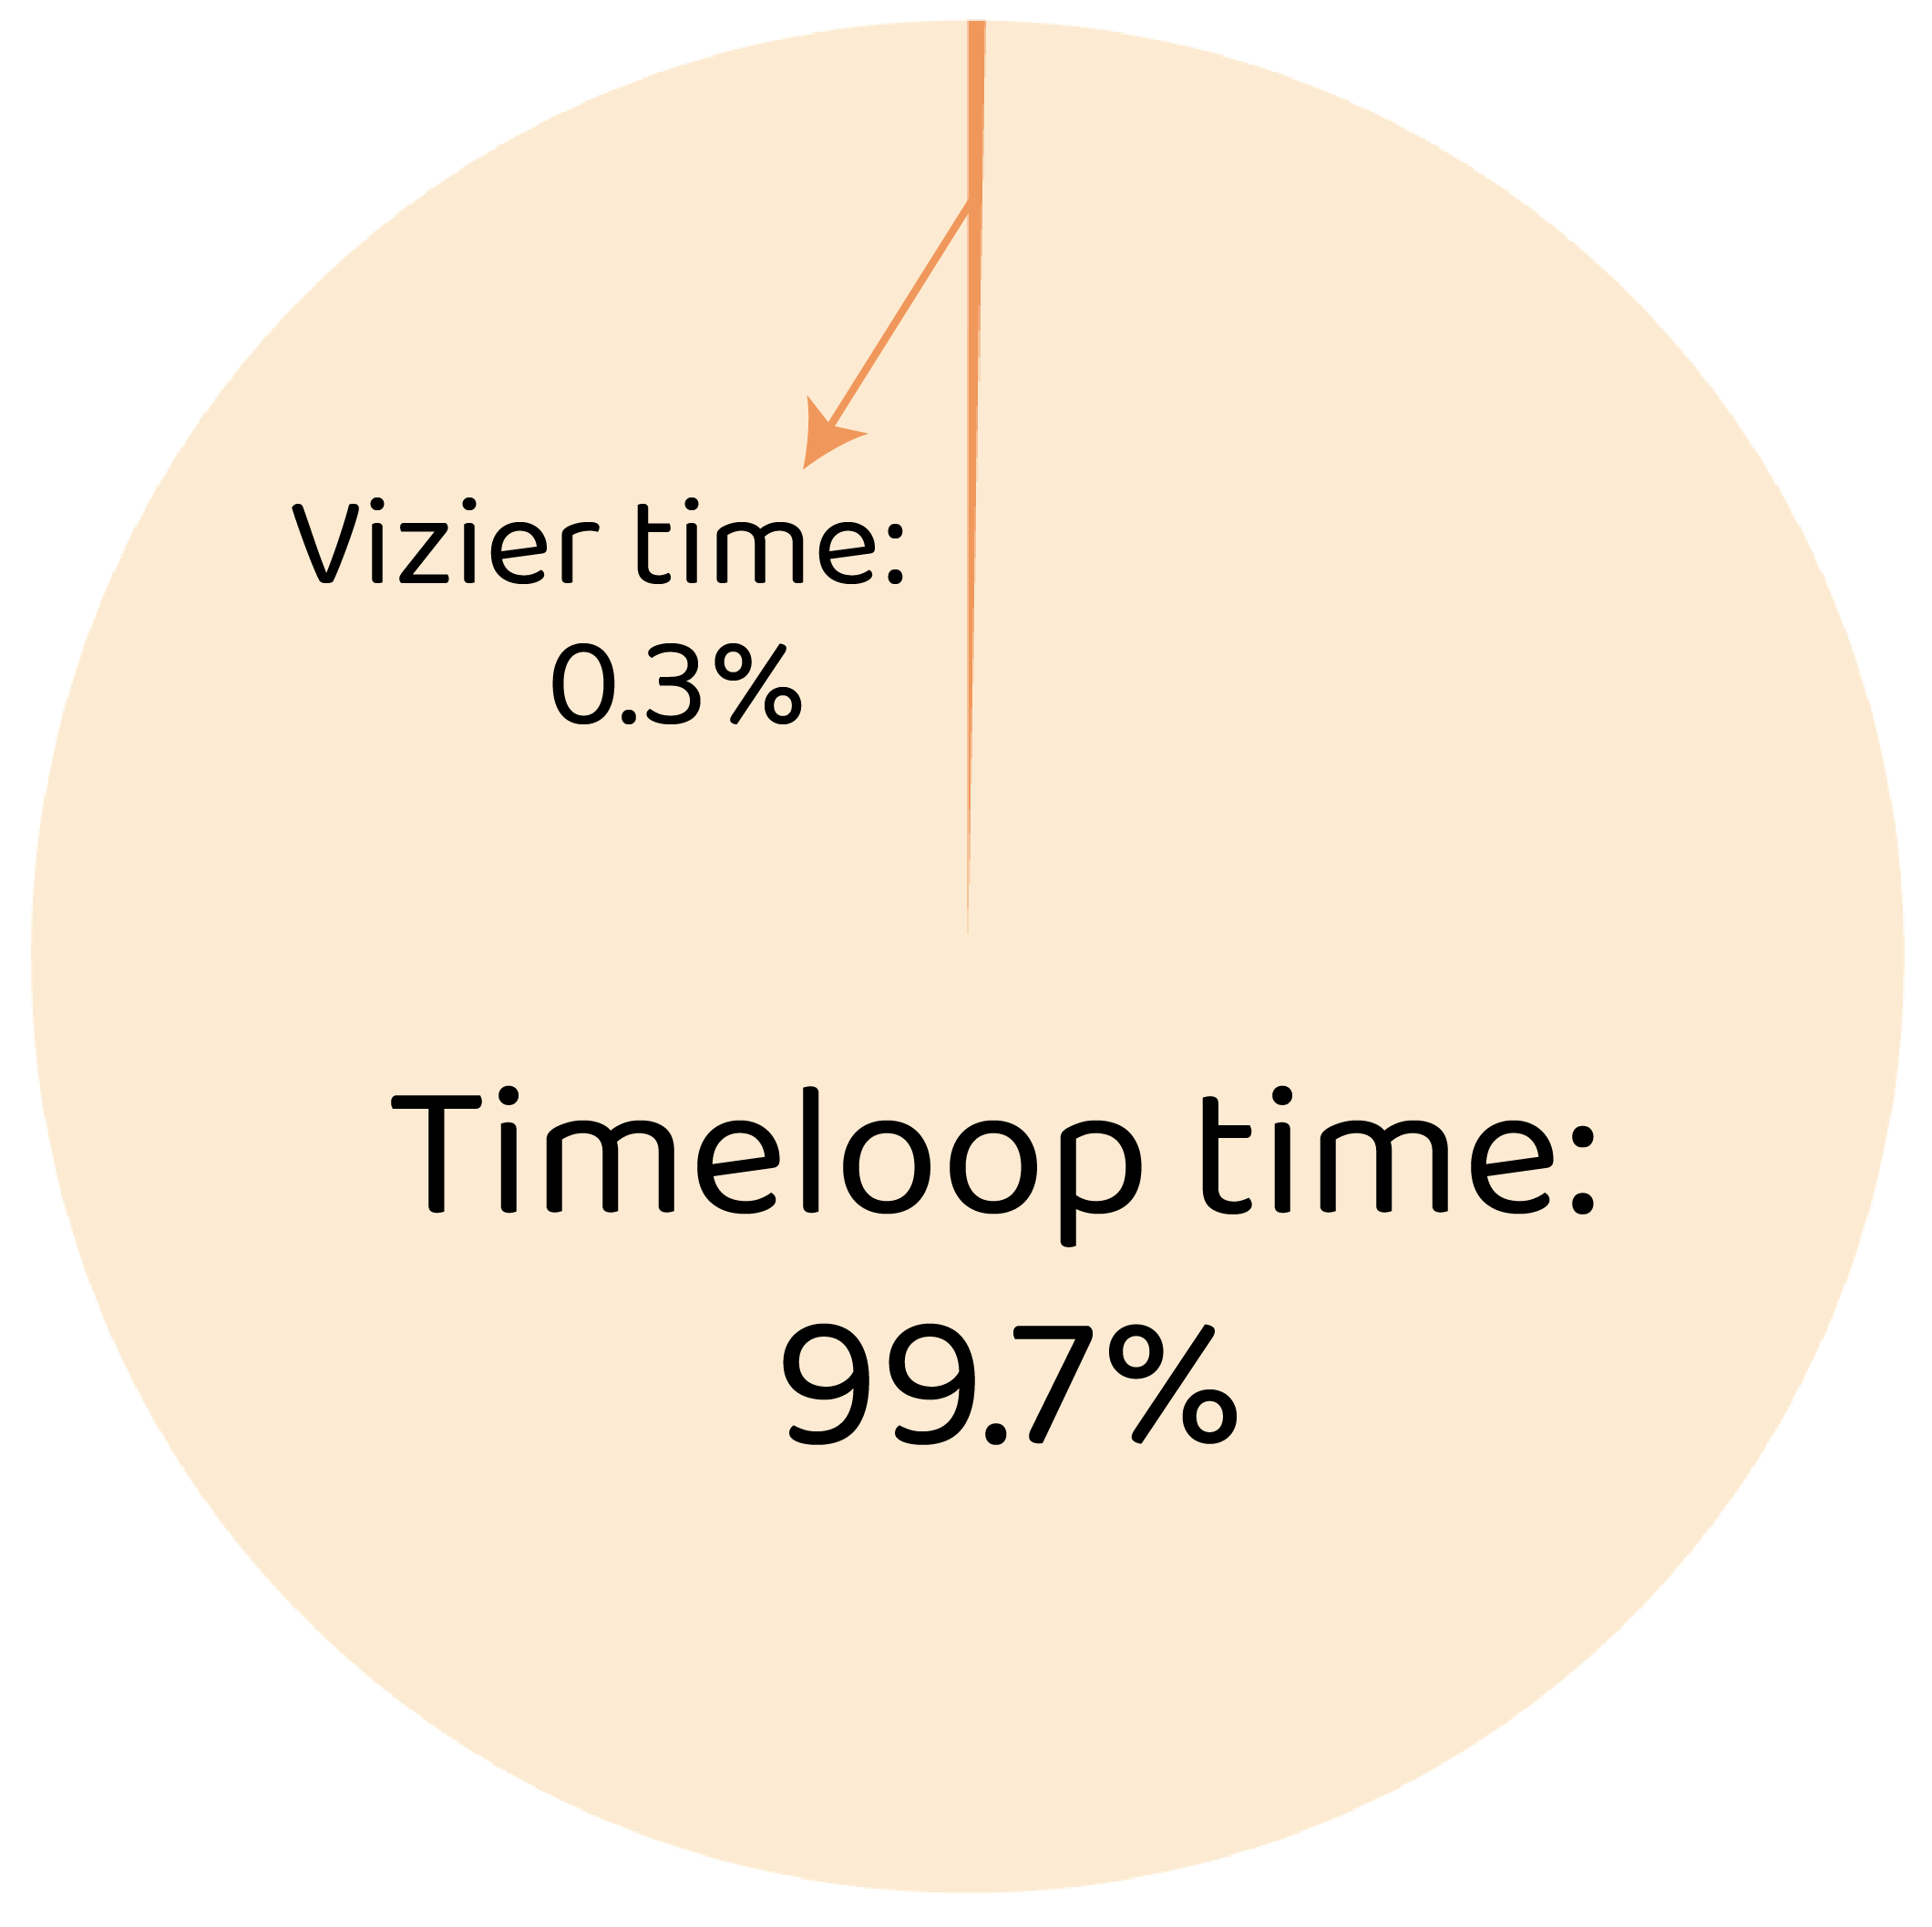
\includegraphics[width=\linewidth]{fig3/timeloop_vs_vizier.png}
%     \caption{Per-trial wall-clock breakdown.}
%     \label{fig:timeloop-time}
%     \vspace{-10pt}
% \end{wrapfigure}
% Despite V0's improvements, it inherits the sequential dependence on external tiling tools (e.g., Timeloop) because it lacks a linear expression for non-linear tiling-fusion interactions. As shown in Figure~\ref{fig:timeloop-time}, Timeloop accounts for over 99\% of per-trial latency, creating a prohibitive bottleneck for multi-thousand-trial searches. To resolve this, CHEETAH-V1 internalizes tiling by precomputing Pareto-pruned configurations and encoding them as decision variables. This removes Timeloop from the critical path, collapsing each trial to a single Vizier-proposal and LP-solve step. We start with introducing the preprocessing stage below before presenting the full formulation.

% % The limitations of prior work is still inherited in the V0 formulation due to the difficulty of expressing non-linear relationships as linear constraints. Therefore tiling decisions $(\Tmax_i, \Tmin_i, t_i^k)$ are fixed constants provided by additional software, such as Timeloop. A natural question is whether this sequential dependence also creates a \emph{runtime} bottleneck. Figure~\ref{fig:timeloop-time} confirms that it does: across different models, Timeloop scheduling on average accounts for over 99\% of per-trial wall-clock time, while the Vizier proposal and fusion ILP together consume less than 1\% on average. Because the outer loop requires thousands of trials to converge, the cumulative cost of repeated Timeloop invocations dominates the total search budget. This observation motivates a key design choice in CHEETAH-V1: rather than calling Timeloop online during each trial, we precompute a Pareto-pruned set of tiling configurations once (Section~\ref{sec:pareto}) and encode the tiling selection as decision variables \emph{inside} the LP. This eliminates Timeloop from the per-trial critical path entirely, reducing each trial to a single Vizier-proposal$\,\to\,$LP-solve step.

% % CHEETAH-V1 captures tiling as a \emph{decision variable} inside the LP, enabling the solver to jointly optimize tiling and fusion. We start with describing our preprocessing stage in Section~\ref{sec:pareto} before presenting the full formulation in Section~\ref{sec::v1}.


% \paragraph{Pareto Pruning Pre-Pass} The raw tiling search space for a $7$-dimensional convolution loop with $3$ memory levels is $\mathcal O(10^7)$ configurations per operation. We reduce this to a tractable Pareto-optimal subset $\mathcal{C}_i$ for each operation $i$ via a pre-pass for (1) L1 feasibility where configurations whose tiled working set exceeds L1 scratchpad capacity $C_{L1}$ are discarded; (2) Pareto optimality where a configuration $c$ is retained only if no other configuration achieves both lower $\Tmax_i(c)$ \emph{and} smaller working-set size in the Global Buffer.

% In practice, Pareto pruning reduces $\mathcal O(10^7)$ raw configurations to $|\mathcal{C}_i| \approx 10^2$ to $10^3$ per operation. Timeloop is run once per (operation, configuration) pair, producing the triple $(\Tmin_i(c), \Tmax_i(c), t_i^k(c))$ for each retained configuration $c \in \mathcal{C}_i$. These are precomputed constants---the LP solver makes no Timeloop calls at solve time. Appendix~\ref{app:details} provides more details.

% \paragraph{Time-invariant Pareto fronts.}
% A key observation is that the Pareto front shape is invariant to memory time: configurations are ranked by compute cycles and working-set bytes, neither of which depends on bandwidth. Changing bandwidth rescales the DRAM access cost $t_i^k(c)$ uniformly. This means the Pareto-pruned configuration sets can be precomputed \emph{once} and reused across all Vizier trials that share the same compute configuration class, amortizing the expensive Timeloop precomputation.

% % \subsubsection{The Joint CHEETAH-V1 LP Formulation}\label{sec::v1}

% \paragraph{From fixed constants to decision variables.}
% V1 brings the tiling choice \emph{inside} the LP by introducing \textbf{tiling selection variables} $y_{i,c} \in [0,1]$, one per Pareto-optimal configuration $c \in \mathcal{C}_i$ from the pre-pass, with the constraint $\sum_c y_{i,c} = 1$ (exactly one configuration is selected per operation). The Timeloop-precomputed constants $\Tmax_i(c)$, $\Tmin_i(c)$, $t_i^k(c)$ now become \emph{per-configuration coefficients} indexed by $c$, so the DRAM savings term becomes $t_i^k(c) \cdot y_{i,c} \cdot p_{\text{assoc}(i,k),\, o(i)}$---a product of \emph{two} decision variables, which is bilinear and cannot be handled by convex programming directly.
 
% % \paragraph{Linearization via McCormick envelopes.}
% % We linearize this product exactly via the classical McCormick substitution. Specifically,  we introduce \textbf{auxiliary variables} $w_{i,c,k} := y_{i,c} \cdot p_{\text{assoc}(i,k),\, o(i)}$ that represent the joint effect of selecting tiling $c$ \emph{and} pinning tensor $k$, constrained by:
% % \begin{equation}
% % \label{eq:mccormick}
% % \begin{aligned}
% %     w_{i,c,k} &\leq y_{i,c}, \qquad
% %     w_{i,c,k} \leq p_{\text{assoc}(i,k),\, o(i)} \\
% %     w_{i,c,k} &\geq y_{i,c} + p_{\text{assoc}(i,k),\, o(i)} - 1, \qquad
% %     w_{i,c,k} \geq 0
% % \end{aligned}
% % \end{equation}
% % Since both factors lie in $[0,1]$, these four constraints force $w_{i,c,k} = y_{i,c} \cdot p$ at any integer vertex, requiring no manually tuned constants. Together, $y_{i,c}$ and $w_{i,c,k}$ account for 1.6M of the 2.08M variables in the \Vone~ LP (Table~\ref{tab:v1_scale}). \todo{change to MoE?}

% \paragraph{Linearization via McCormick envelopes.}
% We linearize this product exactly via the classical McCormick substitution \citep{mccormick1976computability}. Specifically, we introduce \textbf{auxiliary variables} $w_{i,c,k} := y_{i,c} \cdot p_{\text{assoc}(i,k),\, o(i)}$ that represent the joint effect of selecting tiling $c$ \emph{and} pinning tensor $k$, constrained by:
% \vspace{-4pt}
% \begin{equation}
% \label{eq:mccormick}
% \begin{aligned}
%     w_{i,c,k} &\leq y_{i,c}, \qquad
%     w_{i,c,k} \leq p_{\text{assoc}(i,k),\, o(i)} \\
%     w_{i,c,k} &\geq y_{i,c} + p_{\text{assoc}(i,k),\, o(i)} - 1, \qquad
%     w_{i,c,k} \geq 0
% \end{aligned}
% \end{equation}
% Since both factors lie in $[0,1]$, these four constraints force $w_{i,c,k} = y_{i,c} \cdot p$ at any integer vertex, requiring no manually tuned constants. Together, $y_{i,c}$ and $w_{i,c,k}$ constitute the majority of V1's decision variables (Table~\ref{tab:v1_scale}).
% \vspace{-4pt}
% \paragraph{The Joint CHEETAH-V1 LP Formulation.}
% Combining tiling selection, time-indexed placement, rematerialization, and McCormick linearization, the full V1 formulation is:
% \begin{equation}
% \begin{aligned}
% \min \quad & \sum_{i \in \mathcal{N}} T_i + \sum_{i \in \mathcal{N}} \sum_{t \in \mathcal{T}} c_i^{\text{remat}} \, r_{i,t} \\[4pt]
% \text{s.t.} \quad
% & \sum_{c \in \mathcal{C}_i} y_{i,c} = 1 & \forall\, i \in \mathcal{N} \\[3pt]
% & T_i \geq \max\!\left(\sum_{c \in \mathcal{C}_i} \Tmin_i(c)\, y_{i,c},\;\; \sum_{c \in \mathcal{C}_i} \Tmax_i(c)\, y_{i,c} - \sum_{c \in \mathcal{C}_i} \sum_{k} t_i^k(c)\, w_{i,c,k}\right) & \forall\, i \in \mathcal{N} \\[3pt]
% & w_{i,c,k} \leq y_{i,c}, \quad w_{i,c,k} \leq p_{\text{assoc}(i,k),\, o(i)}, \quad w_{i,c,k} \geq y_{i,c} + p_{\text{assoc}(i,k),\, o(i)} - 1 & \forall\, i, c, k \\[3pt]
% & \sum_{e \in \mathcal{E}} d_e\, p_{e,t} + \sum_{i \in \mathcal{N}} d_i^W\, p_{i,t}^W \leq \CGM & \forall\, t \in \mathcal{T} \\[3pt]
% & p_{e,t} \leq p_{e,t-1} + r_{\text{src}(e),\, t} & \forall\, e,\, t > o(\text{src}(e)) \\
% & p_{i,t}^W \leq p_{i,t-1}^W & \forall\, i,\, t > o(i) \\[3pt]
% & r_{i,t} = 0 \;\; \forall\, t \leq o(i); \quad r_{i,t} \leq \min\!\big(p_{e,t},\, p_{i,t}^W\big) \;\; \forall\, e \in \text{in}(i),\, t > o(i) \\[3pt]
% & T_i,\, p_{e,t},\, p_{i,t}^W,\, r_{i,t},\, w_{i,c,k} \geq 0 &
% \end{aligned}
% \tag{V1}\label{eq:v1}
% \end{equation}

% \vspace{-4pt}



% \paragraph{Variable and constraint digest.}
% The V1 formulation inherits all the features of the V0 formulation, and additionally captures tiling by introducing selection variables
% $y_{i,c} \in [0,1]$, constrained by $\sum_c y_{i,c} = 1$, to choose
% from $|\mathcal{C}_i|$ Pareto-optimal configurations.
% Each configuration defines compute costs $T_i^{\max}(c)$,
% $T_i^{\min}(c)$, and per-tensor DRAM savings $t_i^k(c)$.
% We linearize the resulting bilinear DRAM-savings term exactly via
% McCormick auxiliary variables $w_{i,c,k}$, which enforce $w_{i,c,k} \;=\; y_{i,c} \cdot p_{\mathrm{assoc}(i,k),\,o(i)}$ at integer vertices without a relaxation gap. Appendix~\ref{app:lps} describes variables and constraints in detail.

% Per-operation latency $T_i$ is lower-bounded by the weighted
% configuration floor $\sum_c T_i^{\min}(c)\, y_{i,c}$ and the weighted
% off-chip cost $\sum_c T_i^{\max}(c)\, y_{i,c}$ minus achievable savings
% $\sum_{c,k} t_i^k(c)\, w_{i,c,k}$.
% This coupling enables the solver to accept sub-optimal local tiling
% (higher $T_i^{\max}$) if its smaller memory footprint unlocks global
% fusion gains that outweigh the compute-utilization loss.
% Capacity and persistence constraints carry over from V0, utilizing
% edge-indexed placement $p_{e,t}$ to handle multi-fanout nodes.
% For DeepSeek-V3, the V1 LP scales to approximately 2.5M variables,
% 3.0M constraints and 6.1M nonzeros. Table~\ref{tab:v1_scale} provides a representative breakdown; full per-model sizes are in Table~\ref{tab:exp1_lp_sizes} and \ref{tab:exp2_cluster_lp_sizes}. 



% % The V1 formulation extends V0 by making the tiling configuration a decision variable. The selection variables $y_{i,c} \in [0,1]$, with $\sum_c y_{i,c} = 1$, choose among $|\mathcal{C}_i|$ Pareto-optimal tiling configurations precomputed by Timeloop (Section~\ref{sec:pareto}). Each configuration $c$ determines the operation's compute cost $T_i^{\max}(c)$, on-chip floor $T_i^{\min}(c)$, and per-tensor DRAM savings $t_i^k(c)$.
% % The DRAM savings term $t_i^k(c) \cdot y_{i,c} \cdot p_{\text{assoc}(i,k),\,o(i)}$ 
% % is bilinear in the tiling selection and placement variables; we linearize it 
% % via McCormick auxiliary variables $w_{i,c,k}$, constrained by 
% % $w_{i,c,k} \leq y_{i,c}$, $w_{i,c,k} \leq p_{\text{assoc}(i,k),\,o(i)}$, and 
% % $w_{i,c,k} \geq y_{i,c} + p_{\text{assoc}(i,k),\,o(i)} - 1$. 
% % These three inequalities force $w_{i,c,k} = y_{i,c} \cdot p_{\text{assoc}(i,k),\,o(i)}$ 
% % at any integer-feasible point (\cref{prop:mccormick_exact}), so the LP exactly captures the 
% % bilinear interaction without introducing any relaxation gap at integer vertices.
% % The $T_i$ lower bound now takes the maximum of two configuration-dependent terms: the weighted on-chip floor $\sum_c T_i^{\min}(c)\, y_{i,c}$ and the weighted off-chip cost minus achievable savings $\sum_c T_i^{\max}(c)\, y_{i,c} - \sum_{c,k} t_i^k(c)\, w_{i,c,k}$.
% % This coupling is the core novelty of V1: the solver can accept a tiling with higher $T_i^{\max}(c)$ (lower compute utilization) if its smaller working set enables pinning decisions that reduce total DRAM traffic by more than the utilization loss.
% % All remaining constraints---memory capacity, persistence, and rematerialization---carry over from V0 with edge-indexed placement variables $p_{e,t}$ replacing per-tensor $p_{i,t}^k$ to correctly handle skip connections and multi-fanout nodes. For our largest workload, DeepSeek-V3 ($L \approx 6{,}300$ operations), the V1 LP contains approximately 2.5M variables, 3.0M constraints, and 6.1M nonzeros. Table~\ref{tab:v1_scale} provides a representative breakdown; full per-model sizes are in Table~\ref{tab:v1_scale}. 
% % \paragraph{Key constraint interactions.}
% % The execution-time constraints (lines 2--3: the upper and lower bounds for $T_i$) capture the central trade-off that is unique to \Vone: the LP must commit to a tiling configuration $c$ (via $y_{i,c}$) that sets both the baseline compute cost $\Tmax_i(c)$ and the achievable DRAM savings $t_i^k(c)$. A configuration with smaller tiles may have higher $\Tmax_i(c)$ (lower compute utilization) but smaller working sets, enabling more aggressive pinning. The LP balances these trade-offs simultaneously---precisely the cross-stage interaction that the sequential pipeline cannot discover.
 
% % The edge-indexed persistence constraint (line 8: $p_{e,t} \leq p_{e,t-1} + r_{\text{src}(e),\, t}$) and the memory capacity constraint (line 7: lower bound on $\CGM$) are inherited from \Vzero, which introduced per-edge placement variables $p_{e,t}$ to correctly model skip connections. \Vone~ extends this by coupling edge sizes to the tiling selection---since different configurations $c$ produce different activation working sets, the LP can now jointly reason about how tiling choices affect memory pressure across skip connections.




% % \centering
% % \caption{V1 variable and constraint counts (representative, DeepSeek-V3).}
% % \label{tab:v1_scale}
% % \small
% % \begin{tabular}{lrl}
% % \toprule
% % \textbf{Variable} & \textbf{Role} \\
% % \midrule
% % $T_i$ & Per-operation execution time \\
% % $y_{i,c}$ & Tiling configuration selection ($|\mathcal{C}_i|$ options per op) \\
% % $p_{e,t}$ & Edge-indexed activation placement \\
% % $p_{i,t}^W$ & Weight placement \\
% % $r_{i,t}$ & Rematerialization indicator \\
% % $w_{i,c,k}$ & McCormick auxiliaries ($y_{i,c} \cdot p$) \\
% % \midrule
% % \multicolumn{2}{l}{\textbf{DeepSeek-V3 totals} ($L \approx 6{,}300$)} \\
% % \midrule
% % Variables & 2,504,019 \\
% % Constraints & 2,983,450 \\
% % Nonzeros & 6,094,156 \\
% % \bottomrule
% % \end{tabular}
% % \end{table}
% % \paragraph{Comparison across formulations.}
% % Table~\ref{tab:comparison} summarizes the progression from static through V0 to V1.
% % \begin{table}[ht!]
% % \centering
% % \caption{Comparison of static, V0, and V1 formulations.}
% % \label{tab:comparison}
% % \small
% % \begin{tabular}{lccc}
% % \toprule
% % \textbf{Property} & \textbf{static} & \textbf{V0} & \textbf{V1} \\
% % \midrule
% % Joint tiling + fusion & \texttimes & \texttimes & \checkmark \\
% % Time-indexed placement & \texttimes & \checkmark & \checkmark \\
% % Rematerialization & \texttimes & \checkmark & \checkmark \\
% % Relaxed skip connections & \texttimes & Partial & \checkmark \\
% % % Config-dependent DRAM savings & \texttimes & \texttimes & \checkmark \\ 
% % % Bilinear linearization & --- & --- & McCormick \\
% % \bottomrule
% % \end{tabular}
% % \end{table}

% % \paragraph{Structural invariance for efficient LLM integration.}
% % A practical advantage of both our LP formulations is that the constraint matrix sparsity pattern is invariant across hardware configurations---only the numerical coefficients change. This means:
% % \begin{itemize}
% %     \item The LP solver's preconditioner can be designed once per neural network model and reused across all Vizier trials.
% %     \item An LLM-Architect can reason about constraint structure (which constraints are binding, which variables are fractional) without needing to understand the full LP.
% %     \item Warm-starting from a previous trial's LP solution is straightforward since the variable indexing is stable.
% % \end{itemize}

% \begin{wraptable}{r}{0.48\textwidth}
% \vspace{-12pt}   
% \centering
% \caption{V1 variable and constraint counts
% (representative, DeepSeek-V3).}
% \label{tab:v1_scale}
% \footnotesize
% \begin{tabular}{@{}ll@{}}
% \toprule
% \textbf{Variable} & \textbf{Role} \\
% \midrule
% $T_i$       & Per-operation execution time \\
% $y_{i,c}$   & Tiling config selection ($|\mathcal{C}_i|$ options) \\
% $p_{e,t}$   & Edge-indexed activation placement \\
% $p_{i,t}^W$ & Weight placement \\
% $r_{i,t}$   & Rematerialization indicator \\
% $w_{i,c,k}$ & McCormick auxiliaries ($y_{i,c} \cdot p$) \\
% \midrule
% \multicolumn{2}{@{}l}{\textbf{DeepSeek-V3 totals}
%                        ($L \approx 6{,}300$)} \\
% \midrule
% Variables   & $2{,}504{,}019$ \\
% Constraints & $2{,}983{,}450$ \\
% Nonzeros    & $6{,}094{,}156$ \\
% \bottomrule
% \end{tabular}
% \vspace{-14pt} 
% \end{wraptable}

% \vspace{-0.1cm}
% \subsection{Strategic Intelligence: LLM-Guided Outer Search}
% \label{sec:llm_outer}
% \vspace{-0.1cm}
% We use Google Vizier as a black-box Bayesian optimizer to propose hardware configurations. While effective, Vizier requires thousands of iterations to identify suboptimal regions without leveraging structural hardware-workload knowledge. To address this, we introduce an LLM-guided outer-loop controller based on SkyDiscovery that reasons about co-design decisions. This integration is enabled by the CHEETAH-V1 formulation, which removes the Timeloop bottleneck to reduce trial times from days to hours.

% In this hybrid loop, the LLM acts as a \emph{Causal Architect}: it reads a compact \emph{Causal Ledger} of past trials---containing hardware parameters, validity, Perf/TDP, LP duals/slacks, MFU, and roofline diagnostics---and emits a \emph{campaign patch} that constrains Vizier's search to a workload-appropriate architectural neighborhood (e.g., adjusting Global Memory floors, DRAM bandwidth ranges, or systolic shapes). A deterministic \emph{Campaign Validator} clips or rejects each patch to enforce physical constraints (TDP caps, area limits, MAC/bandwidth coupling), preventing the LLM from proposing infeasible regions. Vizier then performs local Bayesian optimization within the approved patch, and the V1 LP evaluates each concrete candidate. A \emph{Roofline Auditor} rejects any result whose predicted latency falls below the physical lower bound $\mathrm{LB} = \max(t_{\text{compute}}, t_{\text{memory}})$. The ledger records each intervention and outcome, preventing redundant exploration. The online Architect is implemented as Qwen2.5-7B-Instruct \citep{qwen25technicalreport} with a LoRA \ref{hu2021lora} adapter trained on past trial logs; a larger teacher model (DeepSeek-V3.2) was used offline for campaign label generation. The full loop details are in Appendix~\ref{app:llm_loop}. We now evaluate the full CHEETAH pipeline---V0, V1, and the LLM Architect---across $11$ vision and language workloads.


% page limit edit

% % \section{Methodology}
% % \label{sec:methods}

% % We present the CHEETAH (\acroletter{C}o-designed \acroletter{H}ardware \acroletter{E}xploration via \acroletter{E}fficient \acroletter{T}hroughput and \acroletter{H}ybrid-search) framework in three parts: Section~\ref{sec:v0} introduces CHEETAH-V0, which extends the static fusion ILP with time-indexed placement and rematerialization. Section~\ref{sec:v1} presents CHEETAH-V1, which jointly optimizes tiling and fusion via McCormick linearization. Section~\ref{sec:llm_outer} describes the LLM-Architect outer loop.


% % % \subsection{\Vzero~: Multi-Period Placement with Rematerialization}
% % \subsection{CHEETAH-V0: Multi-Period Placement with Rematerialization}
% % \label{sec:v0}

% % Our first extension models the neural network's execution as a sequence of $T$ discrete timesteps (one per operation in execution order). This decides at which time, which tensor is pinned, evicted, or recomputed to optimally minimize cycle counts. The key features are:

% % \paragraph{Time-indexed placement.}
% % Instead of a single binary $p_i^k$ per tensor, we introduce $p_{i,t}^k \in [0,1]$ for each tensor $k$ of layer $i$ at each timestep $t$. A tensor can be pinned at timestep $t=5$, and evicted at $t=10$. This models a dynamic memory manager within a single inference pass.

% % \paragraph{Rematerialization.}
% % Rather than always paying DRAM bandwidth to reload an evicted tensor, we introduce variables $r_{i,t} \in [0,1]$ indicating that layer $i$ is recomputed at timestep $t$ to restore its output to the Global Buffer. This is particularly valuable for models such as EfficientNet, where depthwise convolutions account for only ${\sim}5\%$ of total FLOPs but produce large activation tensors. Recomputing a depthwise layer to avoid re-reading 6\,MiB from DRAM at 256\,GB/s can be faster than the DRAM reload itself.

% % \paragraph{Relaxed skip-connection handling.}
% % We lift the limitation of our baseline original ILP, which restricts activation pinning to consecutively-executed operations and limits multi-fanout nodes so that at most one consumer benefits from on-chip data. CHEETAH-V0 uses edge-indexed placement variables $p_{e,t}$ for each edge $e \in \mathcal{E}$ of the dataflow graph, correctly modeling the case where one consumer of a skip connection benefits from on-chip data while another does not.

% % The CHEETAH-V0 LP formulation is:
% % \begin{equation}
% % % \label{eq:v0}
% % \begin{aligned}
% % \min \quad & \sum_{i \in \mathcal{N}} T_i + \sum_{i \in \mathcal{N}} \sum_{t \in \mathcal{T}} c_i^{\text{remat}} \, r_{i,t} \\
% % \text{s.t.} \quad
% % & T_i \geq \Tmax_i - \sum_{k \in \{I,O,W\}} t_i^k \cdot p_{i,o(i)}^k & \forall\, i \in \mathcal{N} \\
% % & T_i \geq \Tmin_i & \forall\, i \in \mathcal{N} \\
% % & \sum_{i \in \mathcal{N}} \sum_{k} d_i^k \, p_{i,t}^k \leq \CGM & \forall\, t \in \mathcal{T} \\
% % & p_{i,t}^k \leq p_{i,t-1}^k + r_{i,t} & \forall\, i, t, k \in \{I,O\} \\
% % & p_{i,t}^W \leq p_{i,t-1}^W & \forall\, i, t \\
% % & r_{i,t} = 0 & \forall\, i, t \leq o(i) \\
% % & 0 \leq p_{i,t}^k, r_{i,t} \leq 1 &
% % \end{aligned}
% % \tag{V0}\label{eq:v0}
% % \end{equation}


% % where $o(i)$ is the execution order of operation $i$, $d_i^k$ is the byte size of tensor $k$ for layer $i$, and $c_i^{\text{remat}}$ is the recomputation cost.

% % \paragraph{Variable and constraint digest.}
% % The V0 objective minimizes the sum of execution times $\sum_i T_i$ and
% % rematerialization costs $c_i^{\text{remat}}\, r_{i,t}$.
% % Per-operation latency $T_i$ is lower-bounded by the physical on-chip
% % floor $T_i^{\min}$ and the off-chip time $T_i^{\max}$ adjusted for DRAM
% % savings $t_i^k \cdot p_{i,o(i)}^k$ from pinned tensors.
% % Placement variables $p_{i,t}^k \in [0,1]$ track Global Memory residency
% % for inputs, outputs, and weights at each timestep, subject to a global
% % capacity constraint $C_{\text{GM}}$. Persistence is governed by $p_{i,t}^k \;\leq\; p_{i,t-1}^k + r_{i,t},$ enforcing that activations are either resident from the previous timestep
% % or recomputed; weight tensors satisfy the stricter monotone constraint
% % $p_{i,t}^W \leq p_{i,t-1}^W$, as weights cannot be rematerialized.
% % Rematerialization $r_{i,t}$ is only permitted post-execution
% % ($t > o(i)$) and requires on-chip availability of both inputs and
% % weights.
% % For DeepSeek-V3 ($L \approx 6{,}300$), this formulation yields a
% % large-scale program with approximately 3.3M variables and 3.7M
% % constraints.


% % % \subsection{\textcolor{skyblue}{V1}: Joint Tiling and Fusion via McCormick Linearization}
% % \subsection{CHEETAH-V1: Joint Tiling and Fusion via McCormick Linearization}
% % \label{sec:v1}

% % \begin{wrapfigure}{r}{0.2\linewidth}
% %     \vspace{-12pt}
% %     \centering
% %     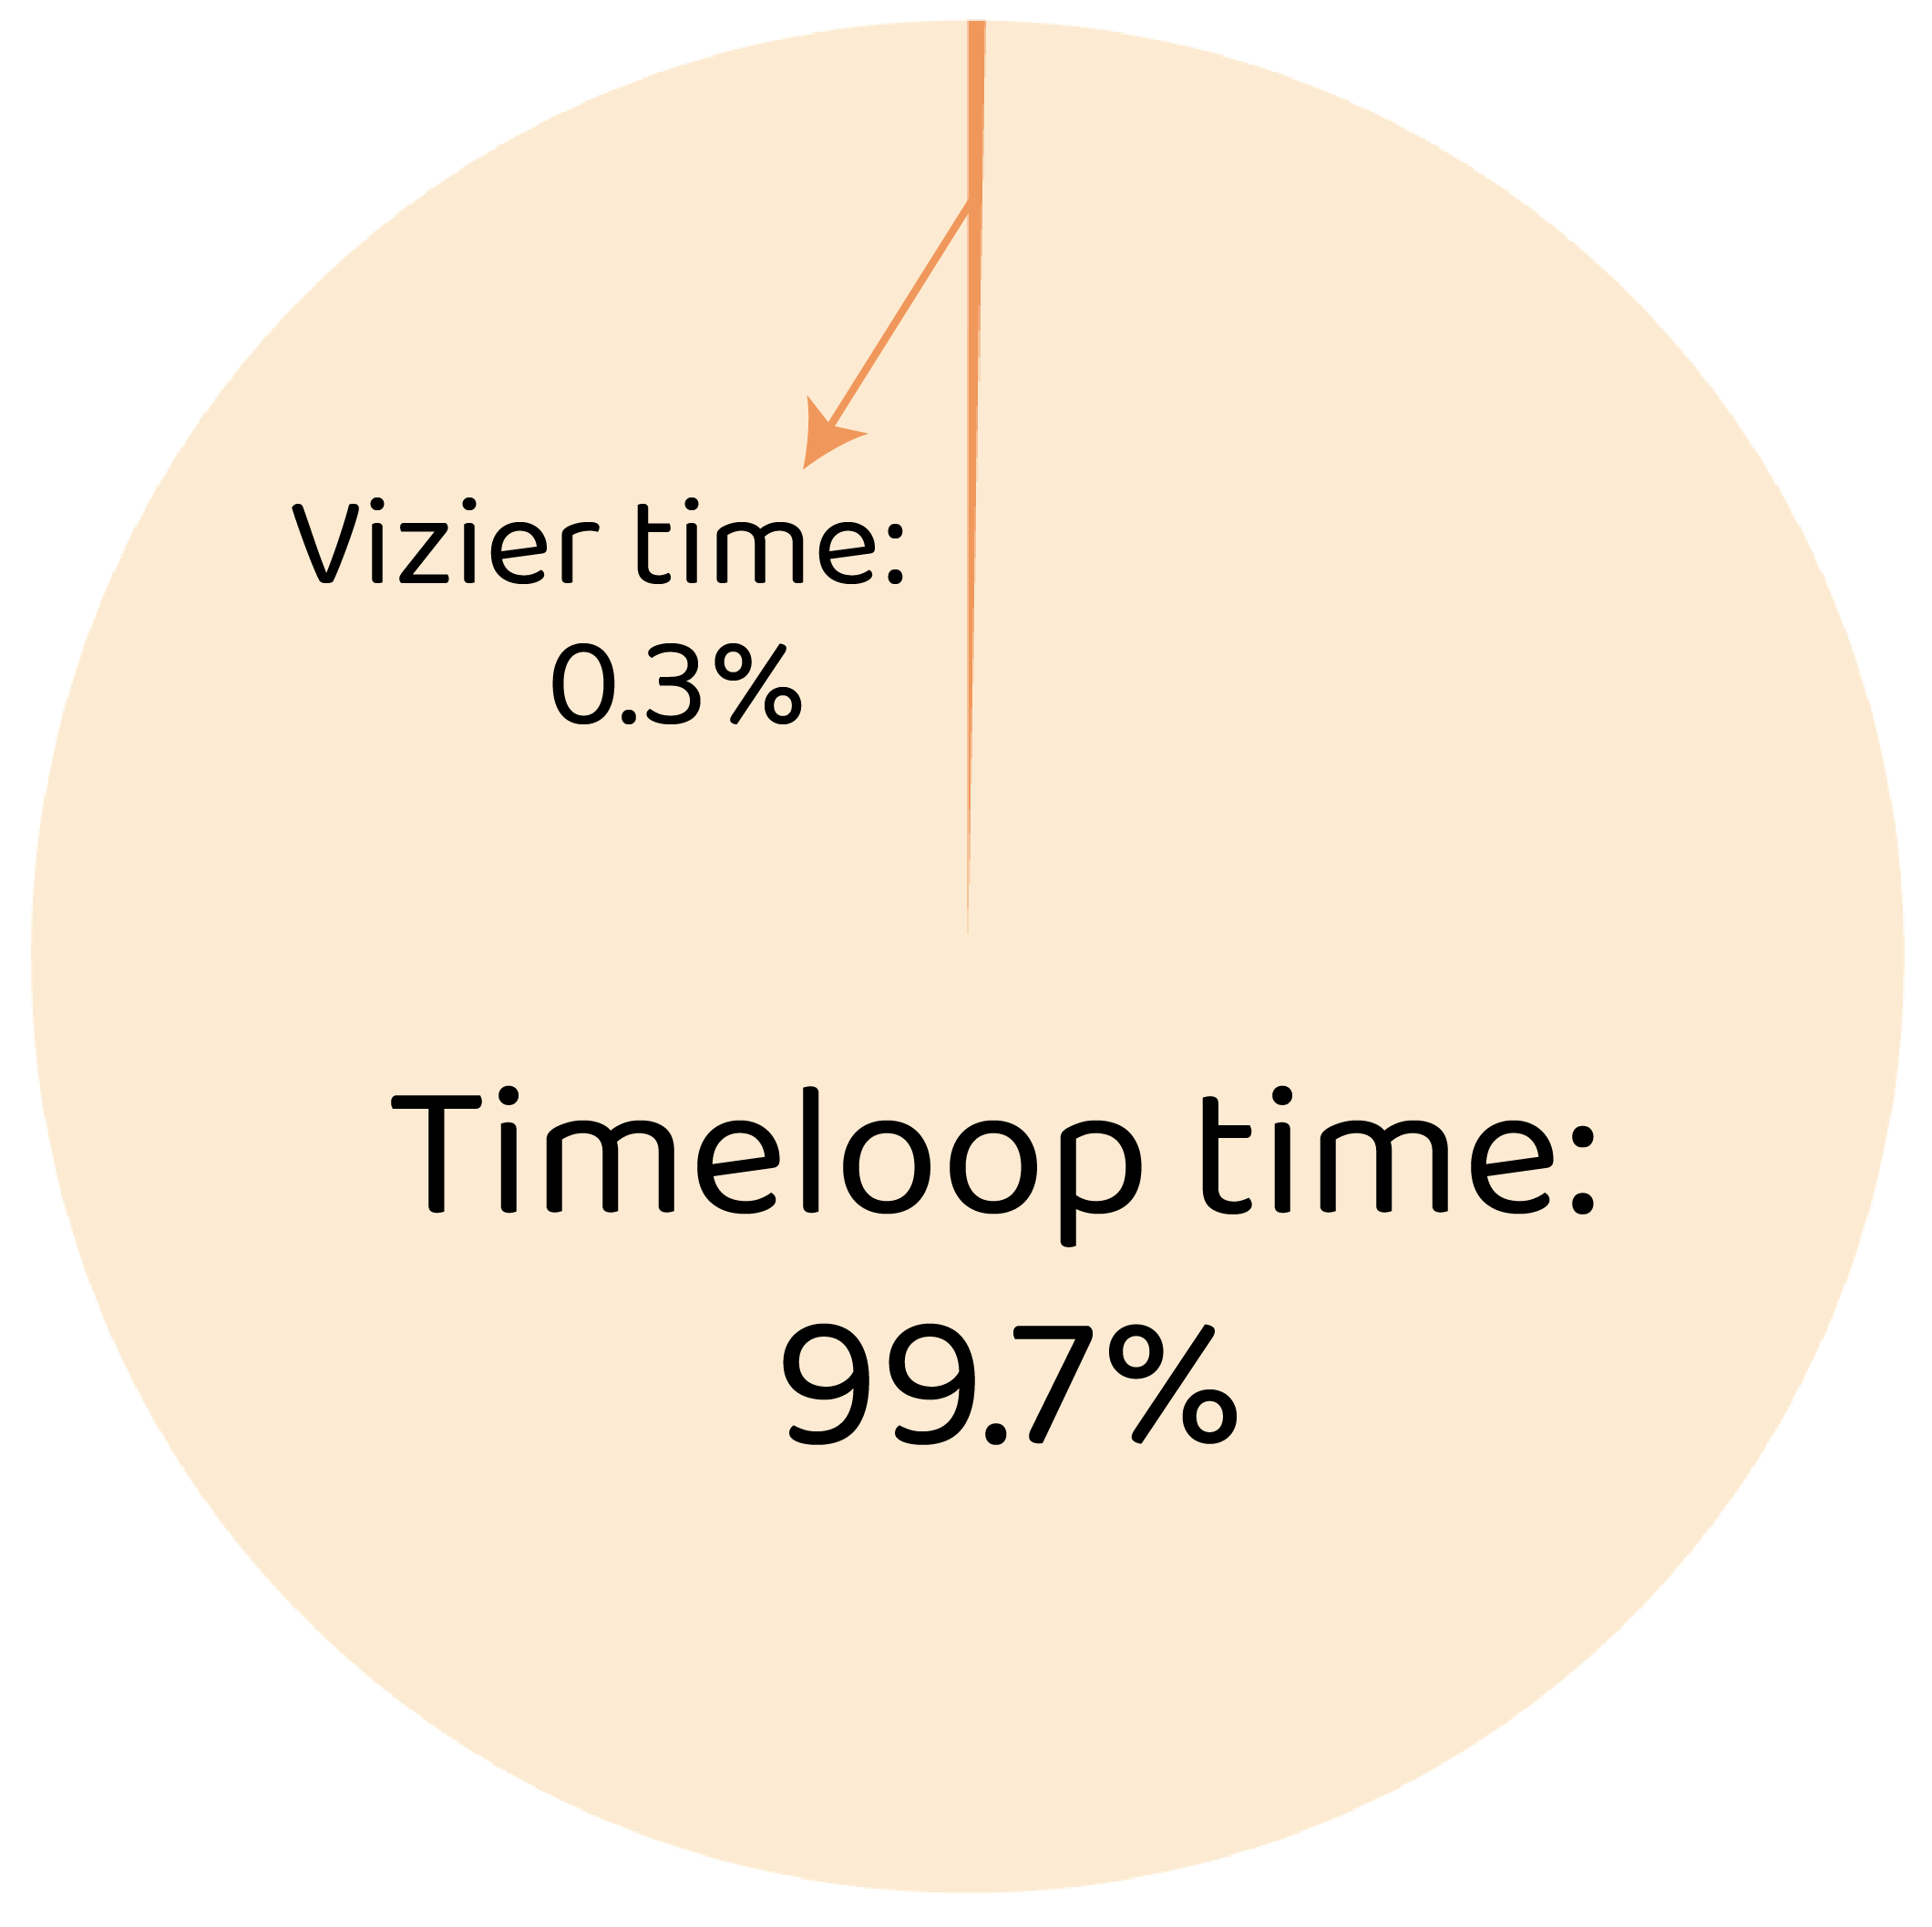
\includegraphics[width=\linewidth]{fig3/timeloop_vs_vizier.png}
% %     \caption{Per-trial wall-clock breakdown.}
% %     \label{fig:timeloop-time}
% %     \vspace{-10pt}
% % \end{wrapfigure}
% % Despite V0's improvements, it inherits the sequential dependence on external tiling tools (e.g., Timeloop) because it lacks a linear expression for non-linear tiling-fusion interactions. As shown in Figure~\ref{fig:timeloop-time}, Timeloop accounts for over 99\% of per-trial latency, creating a prohibitive bottleneck for multi-thousand-trial searches. To resolve this, CHEETAH-V1 internalizes tiling by precomputing Pareto-pruned configurations and encoding them as decision variables. This removes Timeloop from the critical path, collapsing each trial to a single Vizier-proposal and LP-solve step. We start with introducing the preprocessing stage below before presenting the full formulation in Section~\ref{sec::v1}.

% % % The limitations of prior work is still inherited in the V0 formulation due to the difficulty of expressing non-linear relationships as linear constraints. Therefore tiling decisions $(\Tmax_i, \Tmin_i, t_i^k)$ are fixed constants provided by additional software, such as Timeloop. A natural question is whether this sequential dependence also creates a \emph{runtime} bottleneck. Figure~\ref{fig:timeloop-time} confirms that it does: across different models, Timeloop scheduling on average accounts for over 99\% of per-trial wall-clock time, while the Vizier proposal and fusion ILP together consume less than 1\% on average. Because the outer loop requires thousands of trials to converge, the cumulative cost of repeated Timeloop invocations dominates the total search budget. This observation motivates a key design choice in CHEETAH-V1: rather than calling Timeloop online during each trial, we precompute a Pareto-pruned set of tiling configurations once (Section~\ref{sec:pareto}) and encode the tiling selection as decision variables \emph{inside} the LP. This eliminates Timeloop from the per-trial critical path entirely, reducing each trial to a single Vizier-proposal$\,\to\,$LP-solve step.

% % % CHEETAH-V1 captures tiling as a \emph{decision variable} inside the LP, enabling the solver to jointly optimize tiling and fusion. We start with describing our preprocessing stage in Section~\ref{sec:pareto} before presenting the full formulation in Section~\ref{sec::v1}.


% % \paragraph{Pareto Pruning Pre-Pass} The raw tiling search space for a $7$-dimensional convolution loop with $3$ memory levels is $\mathcal O(10^7)$ configurations per operation. We reduce this to a tractable Pareto-optimal subset $\mathcal{C}_i$ for each operation $i$ via a pre-pass for (1) L1 feasibility where configurations whose tiled working set exceeds L1 scratchpad capacity $C_{L1}$ are discarded; (2) Pareto optimality where a configuration $c$ is retained only if no other configuration achieves both lower $\Tmax_i(c)$ \emph{and} smaller working-set size in the Global Buffer.

% % In practice, Pareto pruning reduces $\mathcal O(10^7)$ raw configurations to $|\mathcal{C}_i| \approx 10^2$ to $10^3$ per operation. Timeloop is run once per (operation, configuration) pair, producing the triple $(\Tmin_i(c), \Tmax_i(c), t_i^k(c))$ for each retained configuration $c \in \mathcal{C}_i$. These are precomputed constants---the LP solver makes no Timeloop calls at solve time.

% % \paragraph{Time-invariant Pareto fronts.}
% % A key observation is that the Pareto front shape is invariant to memory time: configurations are ranked by compute cycles and working-set bytes, neither of which depends on bandwidth. Changing bandwidth rescales the DRAM access cost $t_i^k(c)$ uniformly. This means the Pareto-pruned configuration sets can be precomputed \emph{once} and reused across all Vizier trials that share the same compute configuration class, amortizing the expensive Timeloop precomputation.

% % \subsubsection{The Joint CHEETAH-V1 LP Formulation}\label{sec::v1}

% % \paragraph{From fixed constants to decision variables.}
% % In static and V0 formulations, Timeloop selects a single tiling per operation externally and passes the results to the LP as fixed constants $\Tmax_i$, $\Tmin_i$, $t_i^k$. The DRAM savings from pinning tensor $k$ of operation $i$ is then simply $t_i^k \cdot p_{i,o(i)}^k$---a constant times a variable, which is already linear. V1 brings this tiling choice \emph{inside} the LP by introducing \textbf{tiling selection variables} $y_{i,c} \in [0,1]$, one per Pareto-optimal configuration $c \in \mathcal{C}_i$ from the pre-pass, with the constraint $\sum_c y_{i,c} = 1$ (exactly one configuration is selected per operation). The Timeloop-precomputed constants $\Tmax_i(c)$, $\Tmin_i(c)$, $t_i^k(c)$ now become \emph{per-configuration coefficients} indexed by $c$. This means the DRAM savings term becomes $t_i^k(c) \cdot y_{i,c} \cdot p_{\text{assoc}(i,k),\, o(i)}$. This is a product of \emph{two} decision variables, which is bilinear and cannot be handled by a convex programming directly.
 
% % % \paragraph{Linearization via McCormick envelopes.}
% % % We linearize this product exactly via the classical McCormick substitution. Specifically,  we introduce \textbf{auxiliary variables} $w_{i,c,k} := y_{i,c} \cdot p_{\text{assoc}(i,k),\, o(i)}$ that represent the joint effect of selecting tiling $c$ \emph{and} pinning tensor $k$, constrained by:
% % % \begin{equation}
% % % \label{eq:mccormick}
% % % \begin{aligned}
% % %     w_{i,c,k} &\leq y_{i,c}, \qquad
% % %     w_{i,c,k} \leq p_{\text{assoc}(i,k),\, o(i)} \\
% % %     w_{i,c,k} &\geq y_{i,c} + p_{\text{assoc}(i,k),\, o(i)} - 1, \qquad
% % %     w_{i,c,k} \geq 0
% % % \end{aligned}
% % % \end{equation}
% % % Since both factors lie in $[0,1]$, these four constraints force $w_{i,c,k} = y_{i,c} \cdot p$ at any integer vertex, requiring no manually tuned constants. Together, $y_{i,c}$ and $w_{i,c,k}$ account for 1.6M of the 2.08M variables in the \Vone~ LP (Table~\ref{tab:v1_scale}). \todo{change to MoE?}

% % \paragraph{Linearization via McCormick envelopes.}
% % We linearize this product exactly via the classical McCormick substitution \citep{mccormick1976computability}. Specifically, we introduce \textbf{auxiliary variables} $w_{i,c,k} := y_{i,c} \cdot p_{\text{assoc}(i,k),\, o(i)}$ that represent the joint effect of selecting tiling $c$ \emph{and} pinning tensor $k$, constrained by:
% % \begin{equation}
% % \label{eq:mccormick}
% % \begin{aligned}
% %     w_{i,c,k} &\leq y_{i,c}, \qquad
% %     w_{i,c,k} \leq p_{\text{assoc}(i,k),\, o(i)} \\
% %     w_{i,c,k} &\geq y_{i,c} + p_{\text{assoc}(i,k),\, o(i)} - 1, \qquad
% %     w_{i,c,k} \geq 0
% % \end{aligned}
% % \end{equation}
% % Since both factors lie in $[0,1]$, these four constraints force $w_{i,c,k} = y_{i,c} \cdot p$ at any integer vertex, requiring no manually tuned constants. Together, $y_{i,c}$ and $w_{i,c,k}$ constitute the majority of V1's decision variables (Table~\ref{tab:v1_scale}).
 

% % % \paragraph{Full formulation.}
% % % Combining tiling selection, time-indexed placement, rematerialization, and McCormick linearization, the full V1  formulation is:

% % % \begin{equation}
% % % % \label{eq:v1}
% % % \begin{aligned}
% % % \min \quad & \sum_{i \in \mathcal{N}} T_i + \sum_{i \in \mathcal{N}} \sum_{t \in \mathcal{T}} c_i^{\text{remat}} \, r_{i,t} \\[4pt]
% % % \text{s.t.} \quad
% % % & \sum_{c \in \mathcal{C}_i} y_{i,c} = 1 & \forall\, i \in \mathcal{N} \\[3pt]
% % % & T_i \geq \sum_{c \in \mathcal{C}_i} \Tmax_i(c)\, y_{i,c} - \sum_{c \in \mathcal{C}_i} \sum_{k} t_i^k(c)\, w_{i,c,k} & \forall\, i \in \mathcal{N} \\[3pt]
% % % & T_i \geq \sum_{c \in \mathcal{C}_i} \Tmin_i(c)\, y_{i,c} & \forall\, i \in \mathcal{N} \\[3pt]
% % % & w_{i,c,k} \leq y_{i,c} & \forall\, i, c, k \\
% % % & w_{i,c,k} \leq p_{\text{assoc}(i,k),\, o(i)} & \forall\, i, c, k \\
% % % & w_{i,c,k} \geq y_{i,c} + p_{\text{assoc}(i,k),\, o(i)} - 1 & \forall\, i, c, k \\[3pt]
% % % & \sum_{e \in \mathcal{E}} d_e\, p_{e,t} + \sum_{i \in \mathcal{N}} d_i^W\, p_{i,t}^W \leq \CGM & \forall\, t \in \mathcal{T} \\[3pt]
% % % & p_{e,t} \leq p_{e,t-1} + r_{\text{src}(e),\, t} & \forall\, e, t > o(\text{src}(e)) \\
% % % & p_{i,t}^W \leq p_{i,t-1}^W & \forall\, i, t > o(i) \\[3pt]
% % % & r_{i,t} = 0 & \forall\, i, t \leq o(i) \\
% % % & r_{i,t} \leq p_{e,t} & \forall\, e \in \text{in}(i), t > o(i) \\
% % % & r_{i,t} \leq p_{i,t}^W & \forall\, i, t > o(i) \\[3pt]
% % % & T_i, p_{e,t}, p_{i,t}^W, r_{i,t}, w_{i,c,k} \geq 0 &
% % % \end{aligned}
% % % \tag{\textcolor{skyblue}{V1}}\label{eq:v1}
% % % \end{equation}
% % % full formulation below in appendix 
% % % \begin{equation}
% % % \begin{aligned}
% % % \min \quad & \sum_{i \in \mathcal{N}} T_i + \sum_{i \in \mathcal{N}} \sum_{t \in \mathcal{T}} c_i^{\text{remat}} \, r_{i,t} \\[4pt]
% % % \text{s.t.} \quad
% % % & \sum_{c \in \mathcal{C}_i} y_{i,c} = 1 & \forall\, i \in \mathcal{N} \\[3pt]
% % % & T_i \geq \max\!\left(\sum_{c \in \mathcal{C}_i} \Tmin_i(c)\, y_{i,c},\;\; \sum_{c \in \mathcal{C}_i} \Tmax_i(c)\, y_{i,c} - \sum_{c \in \mathcal{C}_i} \sum_{k} t_i^k(c)\, w_{i,c,k}\right) & \forall\, i \in \mathcal{N} \\[3pt]
% % % & w_{i,c,k} \leq y_{i,c}, \quad w_{i,c,k} \leq p_{\text{assoc}(i,k),\, o(i)}, \quad w_{i,c,k} \geq y_{i,c} + p_{\text{assoc}(i,k),\, o(i)} - 1 & \forall\, i, c, k \\[3pt]
% % % & \sum_{e \in \mathcal{E}} d_e\, p_{e,t} + \sum_{i \in \mathcal{N}} d_i^W\, p_{i,t}^W \leq \CGM & \forall\, t \in \mathcal{T} \\[3pt]
% % % & p_{e,t} \leq p_{e,t-1} + r_{\text{src}(e),\, t} & \forall\, e,\, t > o(\text{src}(e)) \\
% % % & p_{i,t}^W \leq p_{i,t-1}^W & \forall\, i,\, t > o(i) \\[3pt]
% % % & r_{i,t} = 0 \;\; \forall\, t \leq o(i); \quad r_{i,t} \leq \min\!\big(p_{e,t},\, p_{i,t}^W\big) \;\; \forall\, e \in \text{in}(i),\, t > o(i) \\[3pt]
% % % & T_i,\, p_{e,t},\, p_{i,t}^W,\, r_{i,t},\, w_{i,c,k} \geq 0 &
% % % \end{aligned}
% % % \tag{\textcolor{skyblue}{V1}}\label{eq:v1}
% % % \end{equation}

% % \paragraph{Variable and constraint digest.}
% % The V1 formulation inherits all the features of the V0 formulation, and additionally captures tiling by introducing selection variables
% % $y_{i,c} \in [0,1]$, constrained by $\sum_c y_{i,c} = 1$, to choose
% % from $|\mathcal{C}_i|$ Pareto-optimal configurations.
% % Each configuration defines compute costs $T_i^{\max}(c)$,
% % $T_i^{\min}(c)$, and per-tensor DRAM savings $t_i^k(c)$.
% % We linearize the resulting bilinear DRAM-savings term exactly via
% % McCormick auxiliary variables $w_{i,c,k}$, which enforce $w_{i,c,k} \;=\; y_{i,c} \cdot p_{\mathrm{assoc}(i,k),\,o(i)}$ at integer vertices without a relaxation gap.

% % Per-operation latency $T_i$ is lower-bounded by the weighted
% % configuration floor $\sum_c T_i^{\min}(c)\, y_{i,c}$ and the weighted
% % off-chip cost $\sum_c T_i^{\max}(c)\, y_{i,c}$ minus achievable savings
% % $\sum_{c,k} t_i^k(c)\, w_{i,c,k}$.
% % This coupling enables the solver to accept sub-optimal local tiling
% % (higher $T_i^{\max}$) if its smaller memory footprint unlocks global
% % fusion gains that outweigh the compute-utilization loss.
% % Capacity and persistence constraints carry over from V0, utilizing
% % edge-indexed placement $p_{e,t}$ to handle multi-fanout nodes.
% % For DeepSeek-V3, the V1 LP scales to approximately $2{,}504{,}019$ variables, $2{,}983{,}450$ constraints, and $6{,}094{,}156$ non-zeros. Table~\ref{tab:v1_scale} provides a representative breakdown, Table~\ref{tab:comparison} summarizes features of each more powerful formulation; full per-model sizes are in Table~\ref{tab:exp1_lp_sizes} and \ref{tab:exp2_cluster_lp_sizes}. 



% % % The V1 formulation extends V0 by making the tiling configuration a decision variable. The selection variables $y_{i,c} \in [0,1]$, with $\sum_c y_{i,c} = 1$, choose among $|\mathcal{C}_i|$ Pareto-optimal tiling configurations precomputed by Timeloop (Section~\ref{sec:pareto}). Each configuration $c$ determines the operation's compute cost $T_i^{\max}(c)$, on-chip floor $T_i^{\min}(c)$, and per-tensor DRAM savings $t_i^k(c)$.
% % % The DRAM savings term $t_i^k(c) \cdot y_{i,c} \cdot p_{\text{assoc}(i,k),\,o(i)}$ 
% % % is bilinear in the tiling selection and placement variables; we linearize it 
% % % via McCormick auxiliary variables $w_{i,c,k}$, constrained by 
% % % $w_{i,c,k} \leq y_{i,c}$, $w_{i,c,k} \leq p_{\text{assoc}(i,k),\,o(i)}$, and 
% % % $w_{i,c,k} \geq y_{i,c} + p_{\text{assoc}(i,k),\,o(i)} - 1$. 
% % % These three inequalities force $w_{i,c,k} = y_{i,c} \cdot p_{\text{assoc}(i,k),\,o(i)}$ 
% % % at any integer-feasible point (\cref{prop:mccormick_exact}), so the LP exactly captures the 
% % % bilinear interaction without introducing any relaxation gap at integer vertices.
% % % The $T_i$ lower bound now takes the maximum of two configuration-dependent terms: the weighted on-chip floor $\sum_c T_i^{\min}(c)\, y_{i,c}$ and the weighted off-chip cost minus achievable savings $\sum_c T_i^{\max}(c)\, y_{i,c} - \sum_{c,k} t_i^k(c)\, w_{i,c,k}$.
% % % This coupling is the core novelty of V1: the solver can accept a tiling with higher $T_i^{\max}(c)$ (lower compute utilization) if its smaller working set enables pinning decisions that reduce total DRAM traffic by more than the utilization loss.
% % % All remaining constraints---memory capacity, persistence, and rematerialization---carry over from V0 with edge-indexed placement variables $p_{e,t}$ replacing per-tensor $p_{i,t}^k$ to correctly handle skip connections and multi-fanout nodes. For our largest workload, DeepSeek-V3 ($L \approx 6{,}300$ operations), the V1 LP contains approximately 2.5M variables, 3.0M constraints, and 6.1M nonzeros. Table~\ref{tab:v1_scale} provides a representative breakdown; full per-model sizes are in Table~\ref{tab:v1_scale}. 
% % % \paragraph{Key constraint interactions.}
% % % The execution-time constraints (lines 2--3: the upper and lower bounds for $T_i$) capture the central trade-off that is unique to \Vone: the LP must commit to a tiling configuration $c$ (via $y_{i,c}$) that sets both the baseline compute cost $\Tmax_i(c)$ and the achievable DRAM savings $t_i^k(c)$. A configuration with smaller tiles may have higher $\Tmax_i(c)$ (lower compute utilization) but smaller working sets, enabling more aggressive pinning. The LP balances these trade-offs simultaneously---precisely the cross-stage interaction that the sequential pipeline cannot discover.
 
% % % The edge-indexed persistence constraint (line 8: $p_{e,t} \leq p_{e,t-1} + r_{\text{src}(e),\, t}$) and the memory capacity constraint (line 7: lower bound on $\CGM$) are inherited from \Vzero, which introduced per-edge placement variables $p_{e,t}$ to correctly model skip connections. \Vone~ extends this by coupling edge sizes to the tiling selection---since different configurations $c$ produce different activation working sets, the LP can now jointly reason about how tiling choices affect memory pressure across skip connections.


% % \begin{figure}[ht!]
% % \begin{minipage}[t]{0.48\textwidth}
% % \vspace{0pt}
% % \centering
% % \captionof{table}{V1 variable and constraint counts
% % (representative, DeepSeek-V3).}
% % \label{tab:v1_scale}
% % \footnotesize
% % \begin{tabular}{@{}ll@{}}
% % \toprule
% % \textbf{Variable} & \textbf{Role} \\
% % \midrule
% % $T_i$       & Per-operation execution time \\
% % $y_{i,c}$   & Tiling config selection ($|\mathcal{C}_i|$ options) \\
% % $p_{e,t}$   & Edge-indexed activation placement \\
% % $p_{i,t}^W$ & Weight placement \\
% % $r_{i,t}$   & Rematerialization indicator \\
% % $w_{i,c,k}$ & McCormick auxiliaries ($y_{i,c} \cdot p$) \\
% % % \midrule
% % % \multicolumn{2}{@{}l}{\textbf{DeepSeek-V3 totals}
% % %                        ($L \approx 6{,}300$)} \\
% % % \midrule
% % % Variables   & $2{,}504{,}019$ \\
% % % Constraints & $2{,}983{,}450$ \\
% % % Nonzeros    & $6{,}094{,}156$ \\
% % \bottomrule
% % \end{tabular}
% % \end{minipage}%
% % \hspace{0.02\textwidth}%
% % \begin{minipage}[t]{0.48\textwidth}
% % \vspace{0pt}
% % \centering
% % \captionof{table}{Comparison of static, V0, and V1 formulations.}
% % \label{tab:comparison}
% % \footnotesize
% % \begin{tabular}{@{}lccc@{}}
% % \toprule
% % \textbf{Property} & \textbf{Static} & \textbf{V0} & \textbf{V1} \\
% % \midrule
% % Joint tiling + fusion    & $\times$ & $\times$   & \checkmark \\
% % Time-indexed placement   & $\times$ & \checkmark & \checkmark \\
% % Rematerialization        & $\times$ & \checkmark & \checkmark \\
% % Relaxed skip connections & $\times$ & Partial    & \checkmark \\
% % \bottomrule
% % \end{tabular}

% % \medskip
% % \raggedright
% % \footnotesize
% % % \textbf{Comparison across formulations.}
% % % Table~\ref{tab:comparison} summarizes the progression from the
% % % static formulation through V0 to V1.
% % \end{minipage}
% % \end{figure}


% % % \begin{table}[ht!]
% % % \centering
% % % \caption{V1 variable and constraint counts (representative, DeepSeek-V3).}
% % % \label{tab:v1_scale}
% % % \small
% % % \begin{tabular}{lrl}
% % % \toprule
% % % \textbf{Variable} & \textbf{Role} \\
% % % \midrule
% % % $T_i$ & Per-operation execution time \\
% % % $y_{i,c}$ & Tiling configuration selection ($|\mathcal{C}_i|$ options per op) \\
% % % $p_{e,t}$ & Edge-indexed activation placement \\
% % % $p_{i,t}^W$ & Weight placement \\
% % % $r_{i,t}$ & Rematerialization indicator \\
% % % $w_{i,c,k}$ & McCormick auxiliaries ($y_{i,c} \cdot p$) \\
% % % \midrule
% % % \multicolumn{2}{l}{\textbf{DeepSeek-V3 totals} ($L \approx 6{,}300$)} \\
% % % \midrule
% % % Variables & 2,504,019 \\
% % % Constraints & 2,983,450 \\
% % % Nonzeros & 6,094,156 \\
% % % \bottomrule
% % % \end{tabular}
% % % \end{table}
% % % \paragraph{Comparison across formulations.}
% % % Table~\ref{tab:comparison} summarizes the progression from static through V0 to V1.
% % % \begin{table}[ht!]
% % % \centering
% % % \caption{Comparison of static, V0, and V1 formulations.}
% % % \label{tab:comparison}
% % % \small
% % % \begin{tabular}{lccc}
% % % \toprule
% % % \textbf{Property} & \textbf{static} & \textbf{V0} & \textbf{V1} \\
% % % \midrule
% % % Joint tiling + fusion & \texttimes & \texttimes & \checkmark \\
% % % Time-indexed placement & \texttimes & \checkmark & \checkmark \\
% % % Rematerialization & \texttimes & \checkmark & \checkmark \\
% % % Relaxed skip connections & \texttimes & Partial & \checkmark \\
% % % % Config-dependent DRAM savings & \texttimes & \texttimes & \checkmark \\ 
% % % % Bilinear linearization & --- & --- & McCormick \\
% % % \bottomrule
% % % \end{tabular}
% % % \end{table}

% % % \paragraph{Structural invariance for efficient LLM integration.}
% % % A practical advantage of both our LP formulations is that the constraint matrix sparsity pattern is invariant across hardware configurations---only the numerical coefficients change. This means:
% % % \begin{itemize}
% % %     \item The LP solver's preconditioner can be designed once per neural network model and reused across all Vizier trials.
% % %     \item An LLM-Architect can reason about constraint structure (which constraints are binding, which variables are fractional) without needing to understand the full LP.
% % %     \item Warm-starting from a previous trial's LP solution is straightforward since the variable indexing is stable.
% % % \end{itemize}

% % \subsection{Strategic Intelligence: LLM-Guided Outer Search}
% % \label{sec:llm_outer}
% % We use Google Vizier as a black-box Bayesian optimizer to propose hardware configurations. While effective, vanilla Vizier treats search as pure function optimization, often requiring thousands of iterations to identify suboptimal regions without leveraging structural hardware-workload knowledge. To address this, we introduce an LLM-guided outer-loop controller based on SkyDiscovery that reasons about co-design decisions. By learning from a causal ledger of past trials and Lagrangian dual signals from the LP solver, the LLM proposes meaningful, constrained search-space candidates. This integration is enabled by the CHEETAH-V1 formulation, which removes the Timeloop bottleneck to reduce trial times from days to hours.The LLM-Architect reduces wasted trials by intelligently steering Vizier’s search without altering the inner solver or its optimality certificates. In this hybrid loop, the LLM determines global architectural regions, Vizier performs local Bayesian optimization within those patches, and the large-scale V1 LP solver evaluates each concrete candidate. The LLM-Architect loop proceeds as follows: 
% % % We use Vizier as a black-box Bayesian optimizer to propose candidate hardware configurations. While effective, Vizier search strategies (LCS, UCB, etc) requires thousands of iterations explore and learn which regions are suboptimal and treats the search as a pure function optimization problem without leveraging structural knowledge about hardware-workload interactions.
% % % We leverage an LLM-guided outer-loop controller that learns from logs of thousands of past co-design trials to propose meaningful search-space candidates for Vizier. This is a SkyDiscovery based outer LLM layer which reasons about hardware-software co-design decisions and learns from a causal ledger of constantly updated logs across trials, as well as feed-back signal such as dual variables through the LP solve. This is possible for CHEETAH-V1 LP formulation, since it removes the Timeloop-in-the-loop constraint, thus reducing the co-design problem from days to hours, and permitting the LLM outer loop. 

% % % The LLM-Architect does not change the inner solver, and retains all the optimal certificates of the V1 LP formulation, but intelligently changes where the Vizier outer hardware optimizer searches to reduce wasted trials. The LLM proposes global decisions to determine constrained regions of the hardware search space; Vizier then performs local Bayesian optimization inside those regions; which then passes downstream into a large scale LP solver for the V1 formulation to evaluate each concrete candidate. The LLM-Architect loop proceeds as follows:

% % \begin{enumerate}[leftmargin=1.6em, itemsep=4pt]

% % \item \textbf{Extraction.}
% % Deterministic scripts summarize recent trials into a \emph{Causal
% % Ledger}. Each record includes hardware parameters, validity, Perf/TDP,
% % LP cycles, capacity duals/slacks, bandwidth sensitivity, MFU, memory
% % utilization, roofline gap, failure class, and LP solver metrics.

% % \item \textbf{Context building.}
% % The last $N$ trials and the Causal Ledger are compressed into a compact
% % JSON context for the Architect. The context emphasizes empirical
% % feasibility, observed invalid regions, best known valid designs, and
% % physical audit signals.

% % \item \textbf{Architect.}
% % The online Architect, implemented as Qwen2.5-7B-Instruct with a LoRA
% % adapter trained on past trial logs, diagnoses the dominant bottleneck
% % and emits a campaign patch. The patch constrains macro-architectural
% % search decisions such as Global Memory, DRAM bandwidth, total MACs,
% % systolic shape, PE grid, and batch size. A larger teacher model,
% % DeepSeek-V3.2, was used offline to generate or critique campaign labels
% % but is not in the live loop.

% % \item \textbf{Campaign validation.}
% % A deterministic validator clips or rejects the LLM patch to enforce
% % legal hardware ranges, TDP and area limits, MAC caps, CGM feasibility
% % floors, compute/bandwidth coupling, and roofline constraints. This
% % prevents the LLM from proposing physically implausible regions such as
% % maximum-MAC/minimum-bandwidth designs.

% % \item \textbf{Local optimization.}
% % Vizier is initialized inside the validated patch and warm-started with
% % prior trials that lie in the same region. Vizier then samples concrete
% % hardware candidates within the approved campaign. The LLM therefore
% % chooses the high-level architectural neighbourhood, while Vizier
% % performs local adaptive optimization.

% % \item \textbf{Unified V1 evaluation.}
% % The large-scale LP solver evaluates each candidate by solving the V1
% % joint tiling-fusion-placement LP using saved Pareto $\mathcal{C}$-sets.
% % It returns the objective, cycles, selected tiling configurations,
% % placement/rematerialization decisions, dual/slack summaries, and
% % solver-quality diagnostics.

% % \item \textbf{Roofline audit.}
% % A deterministic Roofline Auditor checks whether the predicted latency
% % is physically plausible. For each candidate we compute
% % \begin{align}
% %     t_{\text{compute}} &=
% %         \frac{\text{useful FLOPs}}{\text{peak FLOPs/s}},
% %     \qquad
% %     t_{\text{memory}}  =
% %         \frac{\text{post-placement DRAM bytes}}{\text{peak bandwidth}},
% %     \nonumber\\
% %     t_{\text{ideal}}   &=
% %         \max\!\left(t_{\text{compute}},\, t_{\text{memory}}\right).
% %     \label{eq:roofline_audit}
% % \end{align}
% % A candidate is rejected if the solver-reported latency falls below this
% % lower bound, or if MFU or memory utilization exceeds 1.0 within
% % tolerance.

% % \item \textbf{Ledger update.}
% % The loop records the campaign hypothesis, intervention, observed
% % invalid-rate change, MFU change, roofline validity, and best Perf/TDP
% % change. The ledger also records forbidden regions when a campaign
% % produces excessive invalid trials.

% % \end{enumerate}

% % \noindent The Architect receives workload summaries, invalid-rate
% % history, MFU, roofline signals, prior valid regions, normalized LP duals,
% % and bandwidth sensitivities. The system starts from a safe empirically
% % valid patch and permits duals only to make bounded edits, such as raising
% % the CGM floor, increasing bandwidth, reducing MAC count, or changing
% % systolic shapes. The validator rejects any dual-guided patch that
% % excludes known high-performing valid regions or predicts a substantially
% % worse feasible rate. This provides controlled architectural feedback in
% % addition to prompt input.


% % % \todo{Expand this section once the LLM+RL experimental protocol is finalized. Key questions to address: (1) Which LLM is used and how is it prompted? (2) How are LLM proposals integrated with Vizier's Bayesian model? (3) What is the sample efficiency improvement over pure Vizier?}





% % edit for page limit 

% \section{Methodology}
% \label{sec:methods}

% We present the CHEETAH (\acroletter{C}o-designed \acroletter{H}ardware \acroletter{E}xploration via \acroletter{E}fficient \acroletter{T}hroughput and \acroletter{H}ybrid-search) framework in three parts: Section~\ref{sec:v0} introduces CHEETAH-V0, which extends the static fusion ILP with time-indexed placement and rematerialization. Section~\ref{sec:v1} presents CHEETAH-V1, which jointly optimizes tiling and fusion via McCormick linearization. Section~\ref{sec:llm_outer} describes the LLM-Architect outer loop.


% % \subsection{\Vzero~: Multi-Period Placement with Rematerialization}
% \subsection{CHEETAH-V0: Multi-Period Placement with Rematerialization}
% \label{sec:v0}

% Our first extension models the neural network's execution as a sequence of $T$ discrete timesteps (one per operation in execution order). This decides at which time, which tensor is pinned, evicted, or recomputed to optimally minimize cycle counts. The key features are:

% \paragraph{Time-indexed placement.}
% Instead of a single binary $p_i^k$ per tensor, we introduce $p_{i,t}^k \in [0,1]$ for each tensor $k$ of layer $i$ at each timestep $t$. A tensor can be pinned at timestep $t=5$, and evicted at $t=10$. This models a dynamic memory manager within a single inference pass.

% \paragraph{Rematerialization.}
% Rather than always paying DRAM bandwidth to reload an evicted tensor, we introduce variables $r_{i,t} \in [0,1]$ indicating that layer $i$ is recomputed at timestep $t$ to restore its output to the Global Buffer. This is particularly valuable for models such as EfficientNet, where depthwise convolutions account for only ${\sim}5\%$ of total FLOPs but produce large activation tensors. Recomputing a depthwise layer to avoid re-reading 6\,MiB from DRAM at 256\,GB/s can be faster than the DRAM reload itself.

% \paragraph{Relaxed skip-connection handling.}
% We lift the limitation of our baseline original ILP, which restricts activation pinning to consecutively-executed operations and limits multi-fanout nodes so that at most one consumer benefits from on-chip data. CHEETAH-V0 uses edge-indexed placement variables $p_{e,t}$ for each edge $e \in \mathcal{E}$ of the dataflow graph, correctly modeling the case where one consumer of a skip connection benefits from on-chip data while another does not.

% The CHEETAH-V0 LP formulation is:
% \begin{equation}
% % \label{eq:v0}
% \begin{aligned}
% \min \quad & \sum_{i \in \mathcal{N}} T_i + \sum_{i \in \mathcal{N}} \sum_{t \in \mathcal{T}} c_i^{\text{remat}} \, r_{i,t} \\
% \text{s.t.} \quad
% & T_i \geq \Tmax_i - \sum_{k \in \{I,O,W\}} t_i^k \cdot p_{i,o(i)}^k & \forall\, i \in \mathcal{N} \\
% & T_i \geq \Tmin_i & \forall\, i \in \mathcal{N} \\
% & \sum_{i \in \mathcal{N}} \sum_{k} d_i^k \, p_{i,t}^k \leq \CGM & \forall\, t \in \mathcal{T} \\
% & p_{i,t}^k \leq p_{i,t-1}^k + r_{i,t} & \forall\, i, t, k \in \{I,O\} \\
% & p_{i,t}^W \leq p_{i,t-1}^W & \forall\, i, t \\
% & r_{i,t} = 0 & \forall\, i, t \leq o(i) \\
% & 0 \leq p_{i,t}^k, r_{i,t} \leq 1 &
% \end{aligned}
% \tag{V0}\label{eq:v0}
% \end{equation}


% where $o(i)$ is the execution order of operation $i$, $d_i^k$ is the byte size of tensor $k$ for layer $i$, and $c_i^{\text{remat}}$ is the recomputation cost.

% \paragraph{Variable and constraint digest.}
% The V0 objective minimizes the sum of execution times $\sum_i T_i$ and
% rematerialization costs $c_i^{\text{remat}}\, r_{i,t}$.
% Per-operation latency $T_i$ is lower-bounded by the physical on-chip
% floor $T_i^{\min}$ and the off-chip time $T_i^{\max}$ adjusted for DRAM
% savings $t_i^k \cdot p_{i,o(i)}^k$ from pinned tensors.
% Placement variables $p_{i,t}^k \in [0,1]$ track Global Memory residency
% for inputs, outputs, and weights at each timestep, subject to a global
% capacity constraint $C_{\text{GM}}$. Persistence is governed by $p_{i,t}^k \;\leq\; p_{i,t-1}^k + r_{i,t},$ enforcing that activations are either resident from the previous timestep
% or recomputed; weight tensors satisfy the stricter monotone constraint
% $p_{i,t}^W \leq p_{i,t-1}^W$, as weights cannot be rematerialized.
% Rematerialization $r_{i,t}$ is only permitted post-execution
% ($t > o(i)$) and requires on-chip availability of both inputs and
% weights.
% For DeepSeek-V3 ($L \approx 6{,}300$), this formulation yields a
% large-scale program with approximately 3.3M variables and 3.7M
% constraints.


% % \subsection{\textcolor{skyblue}{V1}: Joint Tiling and Fusion via McCormick Linearization}
% \subsection{CHEETAH-V1: Joint Tiling and Fusion via McCormick Linearization}
% \label{sec:v1}

% \begin{wrapfigure}{r}{0.2\linewidth}
%     \vspace{-12pt}
%     \centering
%     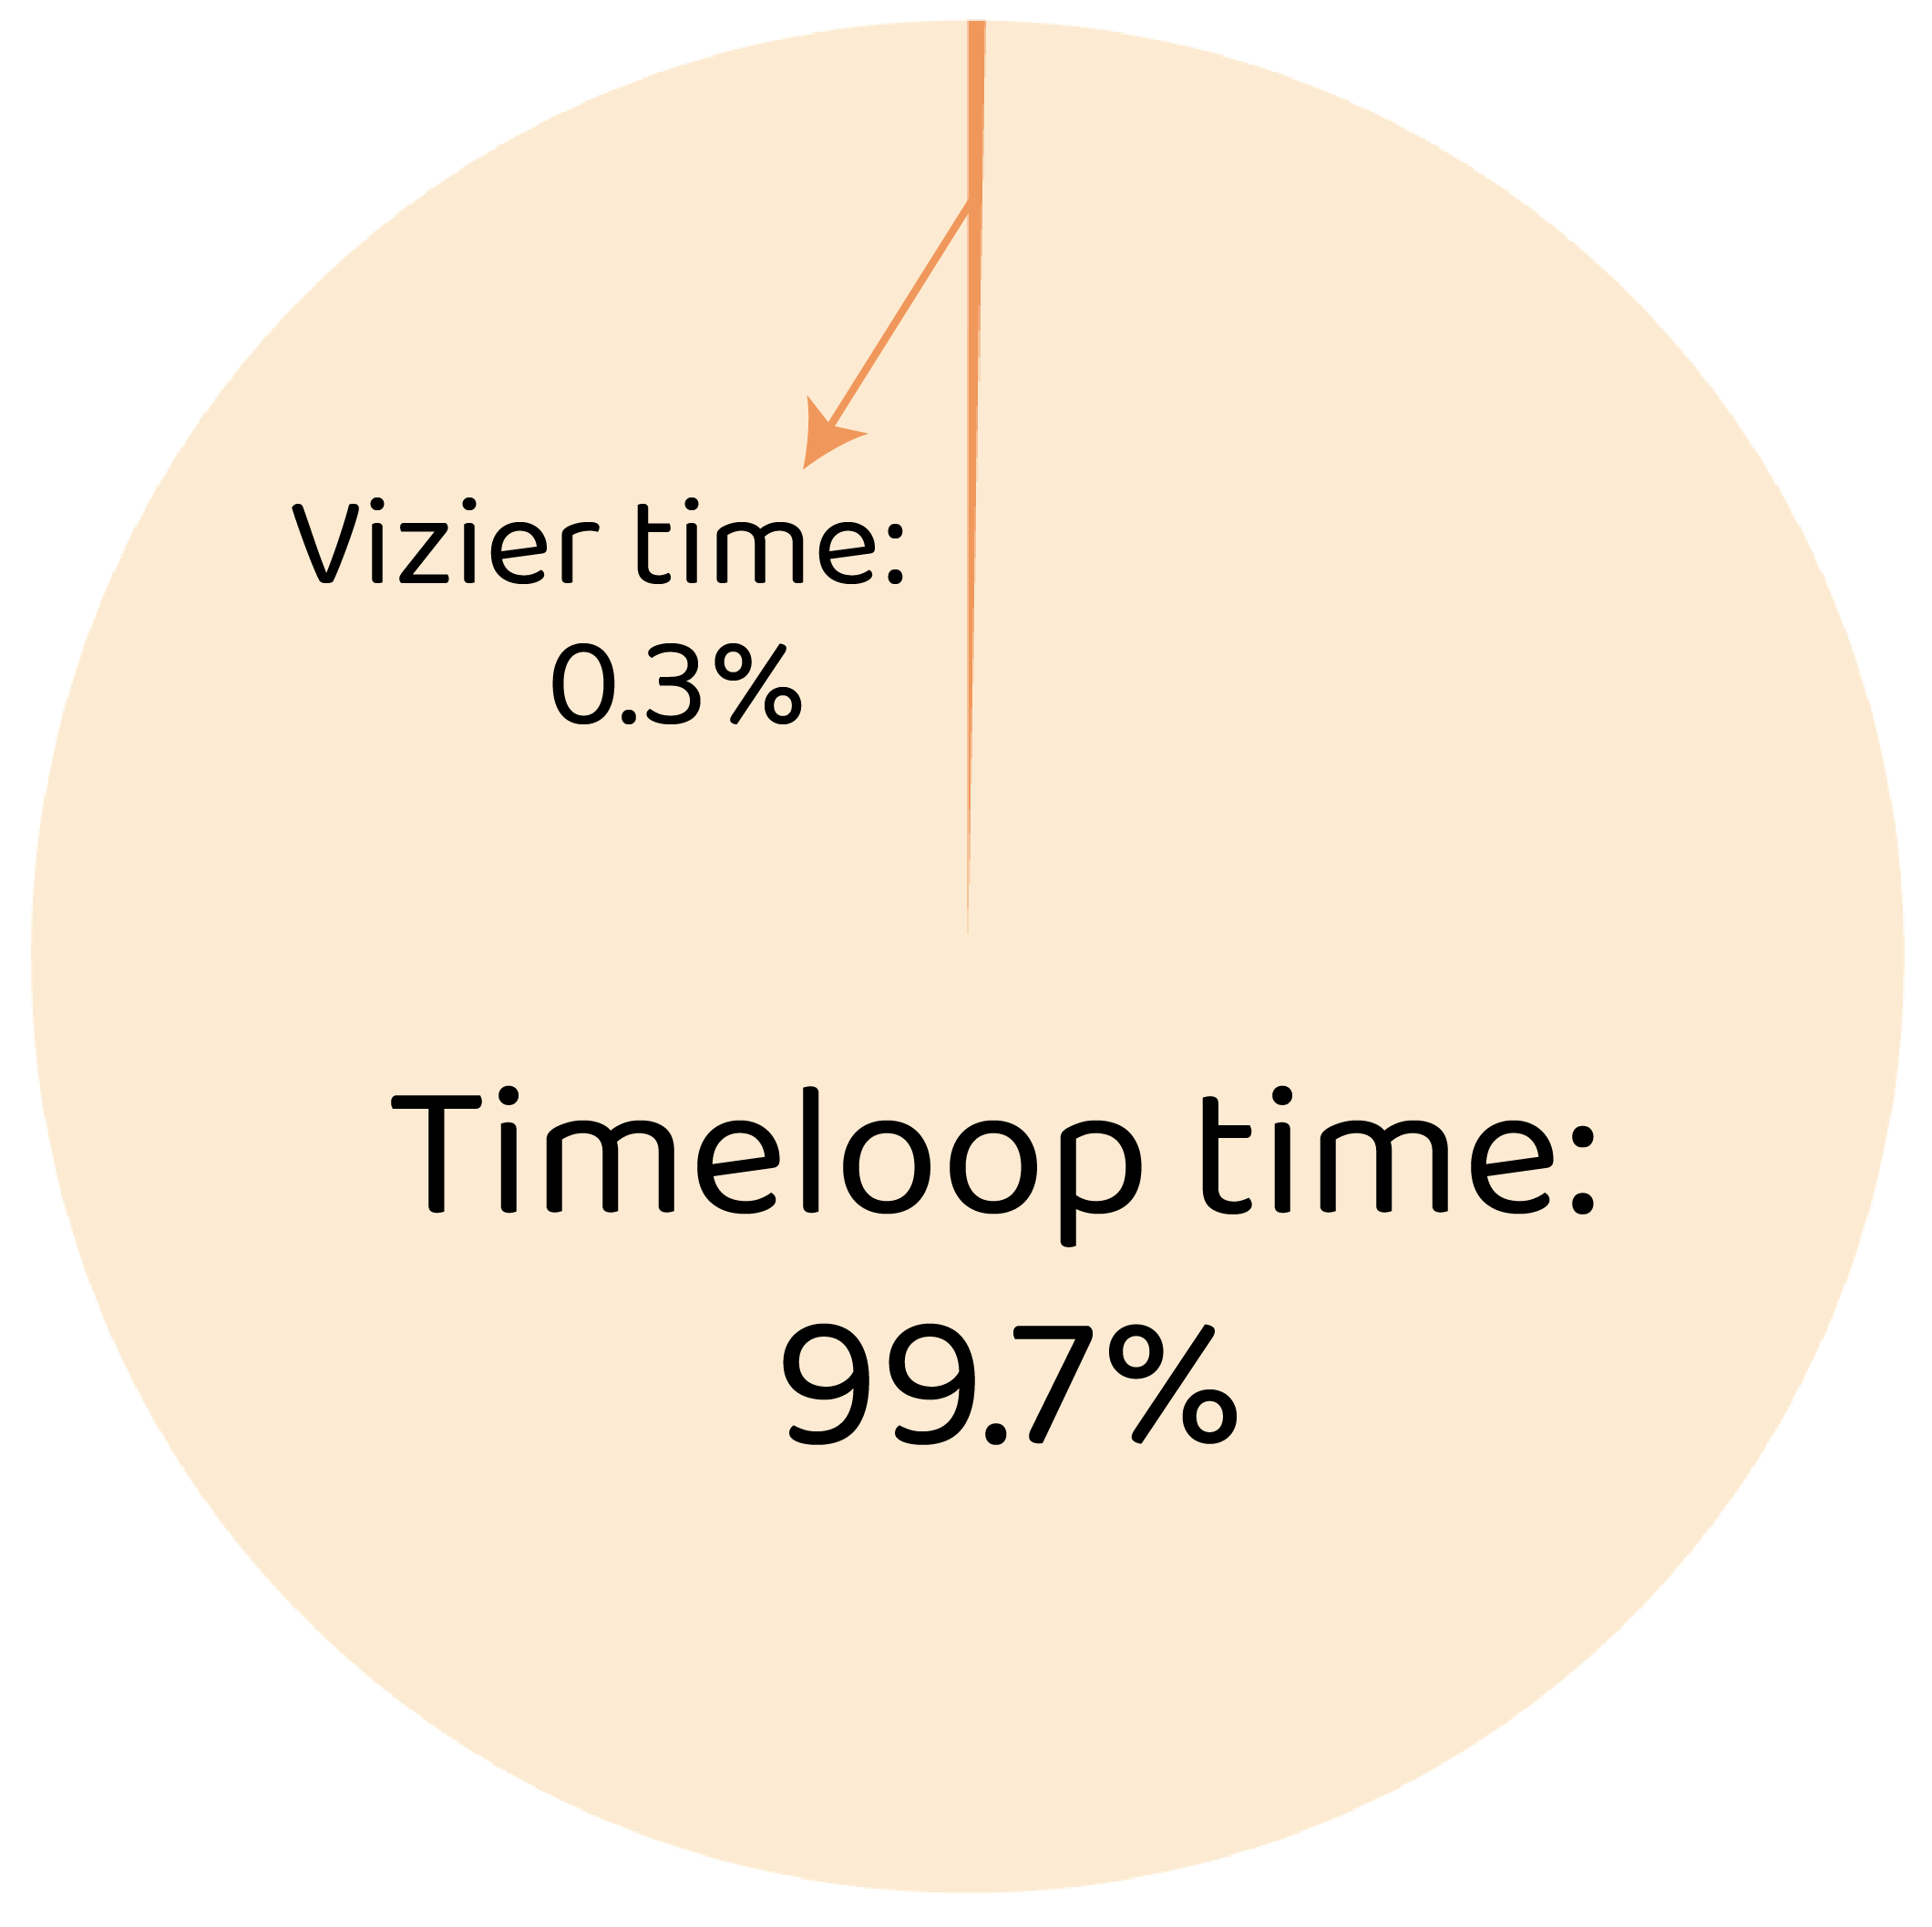
\includegraphics[width=\linewidth]{fig3/timeloop_vs_vizier.png}
%     \caption{Per-trial wall-clock breakdown.}
%     \label{fig:timeloop-time}
%     \vspace{-10pt}
% \end{wrapfigure}
% Despite V0's improvements, it inherits the sequential dependence on external tiling tools (e.g., Timeloop) because it lacks a linear expression for non-linear tiling-fusion interactions. As shown in Figure~\ref{fig:timeloop-time}, Timeloop accounts for over 99\% of per-trial latency, creating a prohibitive bottleneck for multi-thousand-trial searches. To resolve this, CHEETAH-V1 internalizes tiling by precomputing Pareto-pruned configurations and encoding them as decision variables. This removes Timeloop from the critical path, collapsing each trial to a single Vizier-proposal and LP-solve step. We start with introducing the preprocessing stage below before presenting the full formulation in Section~\ref{sec::v1}.

% % The limitations of prior work is still inherited in the V0 formulation due to the difficulty of expressing non-linear relationships as linear constraints. Therefore tiling decisions $(\Tmax_i, \Tmin_i, t_i^k)$ are fixed constants provided by additional software, such as Timeloop. A natural question is whether this sequential dependence also creates a \emph{runtime} bottleneck. Figure~\ref{fig:timeloop-time} confirms that it does: across different models, Timeloop scheduling on average accounts for over 99\% of per-trial wall-clock time, while the Vizier proposal and fusion ILP together consume less than 1\% on average. Because the outer loop requires thousands of trials to converge, the cumulative cost of repeated Timeloop invocations dominates the total search budget. This observation motivates a key design choice in CHEETAH-V1: rather than calling Timeloop online during each trial, we precompute a Pareto-pruned set of tiling configurations once (Section~\ref{sec:pareto}) and encode the tiling selection as decision variables \emph{inside} the LP. This eliminates Timeloop from the per-trial critical path entirely, reducing each trial to a single Vizier-proposal$\,\to\,$LP-solve step.

% % CHEETAH-V1 captures tiling as a \emph{decision variable} inside the LP, enabling the solver to jointly optimize tiling and fusion. We start with describing our preprocessing stage in Section~\ref{sec:pareto} before presenting the full formulation in Section~\ref{sec::v1}.


% \paragraph{Pareto Pruning Pre-Pass.} The raw tiling search space for a $7$-dimensional convolution loop with $3$ memory levels is $\mathcal O(10^7)$ configurations per operation. We reduce this to a tractable Pareto-optimal subset $\mathcal{C}_i$ for each operation $i$ via a pre-pass for (1) L1 feasibility where configurations whose tiled working set exceeds L1 scratchpad capacity $C_{L1}$ are discarded; (2) Pareto optimality where a configuration $c$ is retained only if no other configuration achieves both lower $\Tmax_i(c)$ \emph{and} smaller working-set size in the Global Buffer.

% In practice, Pareto pruning reduces $\mathcal O(10^7)$ raw configurations to $|\mathcal{C}_i| \approx 10^2$ to $10^3$ per operation. Timeloop is run once per (operation, configuration) pair, producing the triple $(\Tmin_i(c), \Tmax_i(c), t_i^k(c))$ for each retained configuration $c \in \mathcal{C}_i$. These are precomputed constants---the LP solver makes no Timeloop calls at solve time.

% \paragraph{Time-invariant Pareto fronts.}
% A key observation is that the Pareto front shape is invariant to memory time: configurations are ranked by compute cycles and working-set bytes, neither of which depends on bandwidth. Changing bandwidth rescales the DRAM access cost $t_i^k(c)$ uniformly. This means the Pareto-pruned configuration sets can be precomputed \emph{once} and reused across all Vizier trials that share the same compute configuration class, amortizing the expensive Timeloop precomputation.

% % \subsubsection{The Joint CHEETAH-V1 LP Formulation}\label{sec::v1}

% \paragraph{From fixed constants to decision variables.}
% In static and V0 formulations, Timeloop selects a single tiling per operation externally and passes the results to the LP as fixed constants $\Tmax_i$, $\Tmin_i$, $t_i^k$. The DRAM savings from pinning tensor $k$ of operation $i$ is then simply $t_i^k \cdot p_{i,o(i)}^k$---a constant times a variable, which is already linear. V1 brings this tiling choice \emph{inside} the LP by introducing \textbf{tiling selection variables} $y_{i,c} \in [0,1]$, one per Pareto-optimal configuration $c \in \mathcal{C}_i$ from the pre-pass, with the constraint $\sum_c y_{i,c} = 1$ (exactly one configuration is selected per operation). The Timeloop-precomputed constants $\Tmax_i(c)$, $\Tmin_i(c)$, $t_i^k(c)$ now become \emph{per-configuration coefficients} indexed by $c$. This means the DRAM savings term becomes $t_i^k(c) \cdot y_{i,c} \cdot p_{\text{assoc}(i,k),\, o(i)}$. This is a product of \emph{two} decision variables, which is bilinear and cannot be handled by a convex programming directly.
 
% % \paragraph{Linearization via McCormick envelopes.}
% % We linearize this product exactly via the classical McCormick substitution. Specifically,  we introduce \textbf{auxiliary variables} $w_{i,c,k} := y_{i,c} \cdot p_{\text{assoc}(i,k),\, o(i)}$ that represent the joint effect of selecting tiling $c$ \emph{and} pinning tensor $k$, constrained by:
% % \begin{equation}
% % \label{eq:mccormick}
% % \begin{aligned}
% %     w_{i,c,k} &\leq y_{i,c}, \qquad
% %     w_{i,c,k} \leq p_{\text{assoc}(i,k),\, o(i)} \\
% %     w_{i,c,k} &\geq y_{i,c} + p_{\text{assoc}(i,k),\, o(i)} - 1, \qquad
% %     w_{i,c,k} \geq 0
% % \end{aligned}
% % \end{equation}
% % Since both factors lie in $[0,1]$, these four constraints force $w_{i,c,k} = y_{i,c} \cdot p$ at any integer vertex, requiring no manually tuned constants. Together, $y_{i,c}$ and $w_{i,c,k}$ account for 1.6M of the 2.08M variables in the \Vone~ LP (Table~\ref{tab:v1_scale}). \todo{change to MoE?}

% \paragraph{Linearization via McCormick envelopes.}
% We linearize this product exactly via the classical McCormick substitution \citep{mccormick1976computability}. Specifically, we introduce \textbf{auxiliary variables} $w_{i,c,k} := y_{i,c} \cdot p_{\text{assoc}(i,k),\, o(i)}$ that represent the joint effect of selecting tiling $c$ \emph{and} pinning tensor $k$, constrained by:
% \begin{equation}
% \label{eq:mccormick}
% \begin{aligned}
%     w_{i,c,k} &\leq y_{i,c}, \qquad
%     w_{i,c,k} \leq p_{\text{assoc}(i,k),\, o(i)} \\
%     w_{i,c,k} &\geq y_{i,c} + p_{\text{assoc}(i,k),\, o(i)} - 1, \qquad
%     w_{i,c,k} \geq 0
% \end{aligned}
% \end{equation}
% Since both factors lie in $[0,1]$, these four constraints force $w_{i,c,k} = y_{i,c} \cdot p$ at any integer vertex, requiring no manually tuned constants. Together, $y_{i,c}$ and $w_{i,c,k}$ constitute the majority of V1's decision variables (Table~\ref{tab:v1_scale}).

% \paragraph{The Joint CHEETAH-V1 LP Formulation.}
% Combining tiling selection, time-indexed placement, rematerialization, and McCormick linearization, the full V1 formulation is:
% \begin{equation}
% \begin{aligned}
% \min \quad & \sum_{i \in \mathcal{N}} T_i + \sum_{i \in \mathcal{N}} \sum_{t \in \mathcal{T}} c_i^{\text{remat}} \, r_{i,t} \\[4pt]
% \text{s.t.} \quad
% & \sum_{c \in \mathcal{C}_i} y_{i,c} = 1 & \forall\, i \in \mathcal{N} \\[3pt]
% & T_i \geq \max\!\left(\sum_{c \in \mathcal{C}_i} \Tmin_i(c)\, y_{i,c},\;\; \sum_{c \in \mathcal{C}_i} \Tmax_i(c)\, y_{i,c} - \sum_{c \in \mathcal{C}_i} \sum_{k} t_i^k(c)\, w_{i,c,k}\right) & \forall\, i \in \mathcal{N} \\[3pt]
% & w_{i,c,k} \leq y_{i,c}, \quad w_{i,c,k} \leq p_{\text{assoc}(i,k),\, o(i)}, \quad w_{i,c,k} \geq y_{i,c} + p_{\text{assoc}(i,k),\, o(i)} - 1 & \forall\, i, c, k \\[3pt]
% & \sum_{e \in \mathcal{E}} d_e\, p_{e,t} + \sum_{i \in \mathcal{N}} d_i^W\, p_{i,t}^W \leq \CGM & \forall\, t \in \mathcal{T} \\[3pt]
% & p_{e,t} \leq p_{e,t-1} + r_{\text{src}(e),\, t} & \forall\, e,\, t > o(\text{src}(e)) \\
% & p_{i,t}^W \leq p_{i,t-1}^W & \forall\, i,\, t > o(i) \\[3pt]
% & r_{i,t} = 0 \;\; \forall\, t \leq o(i); \quad r_{i,t} \leq \min\!\big(p_{e,t},\, p_{i,t}^W\big) \;\; \forall\, e \in \text{in}(i),\, t > o(i) \\[3pt]
% & T_i,\, p_{e,t},\, p_{i,t}^W,\, r_{i,t},\, w_{i,c,k} \geq 0 &
% \end{aligned}
% \tag{V1}\label{eq:v1}
% \end{equation}

% \paragraph{Variable and constraint digest.}
% The V1 formulation inherits all the features of the V0 formulation, and additionally captures tiling by introducing selection variables
% $y_{i,c} \in [0,1]$, constrained by $\sum_c y_{i,c} = 1$, to choose
% from $|\mathcal{C}_i|$ Pareto-optimal configurations.
% Each configuration defines compute costs $T_i^{\max}(c)$,
% $T_i^{\min}(c)$, and per-tensor DRAM savings $t_i^k(c)$.
% We linearize the resulting bilinear DRAM-savings term exactly via
% McCormick auxiliary variables $w_{i,c,k}$, which enforce $w_{i,c,k} \;=\; y_{i,c} \cdot p_{\mathrm{assoc}(i,k),\,o(i)}$ at integer vertices without a relaxation gap.

% Per-operation latency $T_i$ is lower-bounded by the weighted
% configuration floor $\sum_c T_i^{\min}(c)\, y_{i,c}$ and the weighted
% off-chip cost $\sum_c T_i^{\max}(c)\, y_{i,c}$ minus achievable savings
% $\sum_{c,k} t_i^k(c)\, w_{i,c,k}$.
% This coupling enables the solver to accept sub-optimal local tiling
% (higher $T_i^{\max}$) if its smaller memory footprint unlocks global
% fusion gains that outweigh the compute-utilization loss.
% Capacity and persistence constraints carry over from V0, utilizing
% edge-indexed placement $p_{e,t}$ to handle multi-fanout nodes.
% For DeepSeek-V3, the V1 LP scales to approximately 2.5M variables,
% 3.0M constraints and 6.1M nonzeros. Table~\ref{tab:v1_scale} provides a representative breakdown, Table~\ref{tab:comparison} summarizes features of each formulation; full per-model sizes are in Table~\ref{tab:exp1_lp_sizes} and \ref{tab:exp2_cluster_lp_sizes}. 



% % The V1 formulation extends V0 by making the tiling configuration a decision variable. The selection variables $y_{i,c} \in [0,1]$, with $\sum_c y_{i,c} = 1$, choose among $|\mathcal{C}_i|$ Pareto-optimal tiling configurations precomputed by Timeloop (Section~\ref{sec:pareto}). Each configuration $c$ determines the operation's compute cost $T_i^{\max}(c)$, on-chip floor $T_i^{\min}(c)$, and per-tensor DRAM savings $t_i^k(c)$.
% % The DRAM savings term $t_i^k(c) \cdot y_{i,c} \cdot p_{\text{assoc}(i,k),\,o(i)}$ 
% % is bilinear in the tiling selection and placement variables; we linearize it 
% % via McCormick auxiliary variables $w_{i,c,k}$, constrained by 
% % $w_{i,c,k} \leq y_{i,c}$, $w_{i,c,k} \leq p_{\text{assoc}(i,k),\,o(i)}$, and 
% % $w_{i,c,k} \geq y_{i,c} + p_{\text{assoc}(i,k),\,o(i)} - 1$. 
% % These three inequalities force $w_{i,c,k} = y_{i,c} \cdot p_{\text{assoc}(i,k),\,o(i)}$ 
% % at any integer-feasible point (\cref{prop:mccormick_exact}), so the LP exactly captures the 
% % bilinear interaction without introducing any relaxation gap at integer vertices.
% % The $T_i$ lower bound now takes the maximum of two configuration-dependent terms: the weighted on-chip floor $\sum_c T_i^{\min}(c)\, y_{i,c}$ and the weighted off-chip cost minus achievable savings $\sum_c T_i^{\max}(c)\, y_{i,c} - \sum_{c,k} t_i^k(c)\, w_{i,c,k}$.
% % This coupling is the core novelty of V1: the solver can accept a tiling with higher $T_i^{\max}(c)$ (lower compute utilization) if its smaller working set enables pinning decisions that reduce total DRAM traffic by more than the utilization loss.
% % All remaining constraints---memory capacity, persistence, and rematerialization---carry over from V0 with edge-indexed placement variables $p_{e,t}$ replacing per-tensor $p_{i,t}^k$ to correctly handle skip connections and multi-fanout nodes. For our largest workload, DeepSeek-V3 ($L \approx 6{,}300$ operations), the V1 LP contains approximately 2.5M variables, 3.0M constraints, and 6.1M nonzeros. Table~\ref{tab:v1_scale} provides a representative breakdown; full per-model sizes are in Table~\ref{tab:v1_scale}. 
% % \paragraph{Key constraint interactions.}
% % The execution-time constraints (lines 2--3: the upper and lower bounds for $T_i$) capture the central trade-off that is unique to \Vone: the LP must commit to a tiling configuration $c$ (via $y_{i,c}$) that sets both the baseline compute cost $\Tmax_i(c)$ and the achievable DRAM savings $t_i^k(c)$. A configuration with smaller tiles may have higher $\Tmax_i(c)$ (lower compute utilization) but smaller working sets, enabling more aggressive pinning. The LP balances these trade-offs simultaneously---precisely the cross-stage interaction that the sequential pipeline cannot discover.
 
% % The edge-indexed persistence constraint (line 8: $p_{e,t} \leq p_{e,t-1} + r_{\text{src}(e),\, t}$) and the memory capacity constraint (line 7: lower bound on $\CGM$) are inherited from \Vzero, which introduced per-edge placement variables $p_{e,t}$ to correctly model skip connections. \Vone~ extends this by coupling edge sizes to the tiling selection---since different configurations $c$ produce different activation working sets, the LP can now jointly reason about how tiling choices affect memory pressure across skip connections.


% \begin{figure}[ht!]
% \begin{minipage}[t]{0.48\textwidth}
% \vspace{0pt}
% \centering
% \captionof{table}{V1 variable and constraint counts
% (representative, DeepSeek-V3).}
% \label{tab:v1_scale}
% \footnotesize
% \begin{tabular}{@{}ll@{}}
% \toprule
% \textbf{Variable} & \textbf{Role} \\
% \midrule
% $T_i$       & Per-operation execution time \\
% $y_{i,c}$   & Tiling config selection ($|\mathcal{C}_i|$ options) \\
% $p_{e,t}$   & Edge-indexed activation placement \\
% $p_{i,t}^W$ & Weight placement \\
% $r_{i,t}$   & Rematerialization indicator \\
% $w_{i,c,k}$ & McCormick auxiliaries ($y_{i,c} \cdot p$) \\
% % \midrule
% % \multicolumn{2}{@{}l}{\textbf{DeepSeek-V3 totals}
% %                        ($L \approx 6{,}300$)} \\
% % \midrule
% % Variables   & $2{,}504{,}019$ \\
% % Constraints & $2{,}983{,}450$ \\
% % Nonzeros    & $6{,}094{,}156$ \\
% \bottomrule
% \end{tabular}
% \end{minipage}%
% \hspace{0.02\textwidth}%
% \begin{minipage}[t]{0.48\textwidth}
% \vspace{0pt}
% \centering
% \captionof{table}{Comparison of static, V0, and V1 formulations.}
% \label{tab:comparison}
% \footnotesize
% \begin{tabular}{@{}lccc@{}}
% \toprule
% \textbf{Property} & \textbf{Static} & \textbf{V0} & \textbf{V1} \\
% \midrule
% Joint tiling + fusion    & $\times$ & $\times$   & \checkmark \\
% Time-indexed placement   & $\times$ & \checkmark & \checkmark \\
% Rematerialization        & $\times$ & \checkmark & \checkmark \\
% Relaxed skip connections & $\times$ & Partial    & \checkmark \\
% \bottomrule
% \end{tabular}

% \medskip
% \raggedright
% \footnotesize
% % \textbf{Comparison across formulations.}
% % Table~\ref{tab:comparison} summarizes the progression from the
% % static formulation through V0 to V1.
% \end{minipage}
% \end{figure}


% % \begin{table}[ht!]
% % \centering
% % \caption{V1 variable and constraint counts (representative, DeepSeek-V3).}
% % \label{tab:v1_scale}
% % \small
% % \begin{tabular}{lrl}
% % \toprule
% % \textbf{Variable} & \textbf{Role} \\
% % \midrule
% % $T_i$ & Per-operation execution time \\
% % $y_{i,c}$ & Tiling configuration selection ($|\mathcal{C}_i|$ options per op) \\
% % $p_{e,t}$ & Edge-indexed activation placement \\
% % $p_{i,t}^W$ & Weight placement \\
% % $r_{i,t}$ & Rematerialization indicator \\
% % $w_{i,c,k}$ & McCormick auxiliaries ($y_{i,c} \cdot p$) \\
% % \midrule
% % \multicolumn{2}{l}{\textbf{DeepSeek-V3 totals} ($L \approx 6{,}300$)} \\
% % \midrule
% % Variables & 2,504,019 \\
% % Constraints & 2,983,450 \\
% % Nonzeros & 6,094,156 \\
% % \bottomrule
% % \end{tabular}
% % \end{table}
% % \paragraph{Comparison across formulations.}
% % Table~\ref{tab:comparison} summarizes the progression from static through V0 to V1.
% % \begin{table}[ht!]
% % \centering
% % \caption{Comparison of static, V0, and V1 formulations.}
% % \label{tab:comparison}
% % \small
% % \begin{tabular}{lccc}
% % \toprule
% % \textbf{Property} & \textbf{static} & \textbf{V0} & \textbf{V1} \\
% % \midrule
% % Joint tiling + fusion & \texttimes & \texttimes & \checkmark \\
% % Time-indexed placement & \texttimes & \checkmark & \checkmark \\
% % Rematerialization & \texttimes & \checkmark & \checkmark \\
% % Relaxed skip connections & \texttimes & Partial & \checkmark \\
% % % Config-dependent DRAM savings & \texttimes & \texttimes & \checkmark \\ 
% % % Bilinear linearization & --- & --- & McCormick \\
% % \bottomrule
% % \end{tabular}
% % \end{table}

% % \paragraph{Structural invariance for efficient LLM integration.}
% % A practical advantage of both our LP formulations is that the constraint matrix sparsity pattern is invariant across hardware configurations---only the numerical coefficients change. This means:
% % \begin{itemize}
% %     \item The LP solver's preconditioner can be designed once per neural network model and reused across all Vizier trials.
% %     \item An LLM-Architect can reason about constraint structure (which constraints are binding, which variables are fractional) without needing to understand the full LP.
% %     \item Warm-starting from a previous trial's LP solution is straightforward since the variable indexing is stable.
% % \end{itemize}

% \subsection{Strategic Intelligence: LLM-Guided Outer Search}
% \label{sec:llm_outer}
% We use Google Vizier as a black-box Bayesian optimizer to propose hardware configurations. While effective, vanilla Vizier treats search as pure function optimization, often requiring thousands of iterations to identify suboptimal regions without leveraging structural hardware-workload knowledge. To address this, we introduce an LLM-guided outer-loop controller based on SkyDiscovery that reasons about co-design decisions. This integration is enabled by the CHEETAH-V1 formulation, which removes the Timeloop bottleneck to reduce trial times from days to hours.

% In this hybrid loop, the LLM acts as a \emph{Causal Architect}: it reads a compact \emph{Causal Ledger} of past trials---containing hardware parameters, validity, Perf/TDP, LP duals/slacks, MFU, and roofline diagnostics---and emits a \emph{campaign patch} that constrains Vizier's search to a workload-appropriate architectural neighborhood (e.g., adjusting Global Memory floors, DRAM bandwidth ranges, or systolic shapes). A deterministic \emph{Campaign Validator} clips or rejects each patch to enforce physical constraints (TDP caps, area limits, MAC/bandwidth coupling), preventing the LLM from proposing implausible regions. Vizier then performs local Bayesian optimization within the approved patch, and the V1 LP evaluates each concrete candidate. A \emph{Roofline Auditor} rejects any result whose predicted latency falls below the physical lower bound $\mathrm{LB} = \max(t_{\text{compute}}, t_{\text{memory}})$. The ledger records each intervention and outcome, preventing redundant exploration and ensuring full auditability. The online Architect is implemented as Qwen2.5-7B-Instruct with a LoRA adapter trained on past trial logs; a larger teacher model (DeepSeek-V3.2) was used offline for campaign label generation. The full loop details are in Appendix~\ref{app:llm_loop}.


% page edit

% \section{Methodology}
% \label{sec:methods}

% We present the CHEETAH (\acroletter{C}o-designed \acroletter{H}ardware \acroletter{E}xploration via \acroletter{E}fficient \acroletter{T}hroughput and \acroletter{H}ybrid-search) framework in three parts: Section~\ref{sec:v0} introduces CHEETAH-V0, which extends the static fusion ILP with time-indexed placement and rematerialization. Section~\ref{sec:v1} presents CHEETAH-V1, which jointly optimizes tiling and fusion via McCormick linearization. Section~\ref{sec:llm_outer} describes the LLM-Architect outer loop.


% % \subsection{\Vzero~: Multi-Period Placement with Rematerialization}
% \subsection{CHEETAH-V0: Multi-Period Placement with Rematerialization}
% \label{sec:v0}

% Our first extension models the neural network's execution as a sequence of $T$ discrete timesteps (one per operation in execution order). This decides at which time, which tensor is pinned, evicted, or recomputed to optimally minimize cycle counts. The key features are:

% \paragraph{Time-indexed placement.}
% Instead of a single binary $p_i^k$ per tensor, we introduce $p_{i,t}^k \in [0,1]$ for each tensor $k$ of layer $i$ at each timestep $t$. A tensor can be pinned at timestep $t=5$, and evicted at $t=10$. This models a dynamic memory manager within a single inference pass.

% \paragraph{Rematerialization.}
% Rather than always paying DRAM bandwidth to reload an evicted tensor, we introduce variables $r_{i,t} \in [0,1]$ indicating that layer $i$ is recomputed at timestep $t$ to restore its output to the Global Buffer. This is particularly valuable for models such as EfficientNet, where depthwise convolutions account for only ${\sim}5\%$ of total FLOPs but produce large activation tensors. Recomputing a depthwise layer to avoid re-reading 6\,MiB from DRAM at 256\,GB/s can be faster than the DRAM reload itself.

% \paragraph{Relaxed skip-connection handling.}
% We lift the limitation of our baseline original ILP, which restricts activation pinning to consecutively-executed operations and limits multi-fanout nodes so that at most one consumer benefits from on-chip data. CHEETAH-V0 uses edge-indexed placement variables $p_{e,t}$ for each edge $e \in \mathcal{E}$ of the dataflow graph, correctly modeling the case where one consumer of a skip connection benefits from on-chip data while another does not.

% The CHEETAH-V0 LP formulation is:
% \begin{equation}
% % \label{eq:v0}
% \begin{aligned}
% \min \quad & \sum_{i \in \mathcal{N}} T_i + \sum_{i \in \mathcal{N}} \sum_{t \in \mathcal{T}} c_i^{\text{remat}} \, r_{i,t} \\
% \text{s.t.} \quad
% & T_i \geq \Tmax_i - \sum_{k \in \{I,O,W\}} t_i^k \cdot p_{i,o(i)}^k & \forall\, i \in \mathcal{N} \\
% & T_i \geq \Tmin_i & \forall\, i \in \mathcal{N} \\
% & \sum_{i \in \mathcal{N}} \sum_{k} d_i^k \, p_{i,t}^k \leq \CGM & \forall\, t \in \mathcal{T} \\
% & p_{i,t}^k \leq p_{i,t-1}^k + r_{i,t} & \forall\, i, t, k \in \{I,O\} \\
% & p_{i,t}^W \leq p_{i,t-1}^W & \forall\, i, t \\
% & r_{i,t} = 0 & \forall\, i, t \leq o(i) \\
% & 0 \leq p_{i,t}^k, r_{i,t} \leq 1 &
% \end{aligned}
% \tag{V0}\label{eq:v0}
% \end{equation}


% where $o(i)$ is the execution order of operation $i$, $d_i^k$ is the byte size of tensor $k$ for layer $i$, and $c_i^{\text{remat}}$ is the recomputation cost.

% \paragraph{Variable and constraint digest.}
% The V0 objective minimizes the sum of execution times $\sum_i T_i$ and
% rematerialization costs $c_i^{\text{remat}}\, r_{i,t}$.
% Per-operation latency $T_i$ is lower-bounded by the physical on-chip
% floor $T_i^{\min}$ and the off-chip time $T_i^{\max}$ adjusted for DRAM
% savings $t_i^k \cdot p_{i,o(i)}^k$ from pinned tensors.
% Placement variables $p_{i,t}^k \in [0,1]$ track Global Memory residency
% for inputs, outputs, and weights at each timestep, subject to a global
% capacity constraint $C_{\text{GM}}$. Persistence is governed by $p_{i,t}^k \;\leq\; p_{i,t-1}^k + r_{i,t},$ enforcing that activations are either resident from the previous timestep
% or recomputed; weight tensors satisfy the stricter monotone constraint
% $p_{i,t}^W \leq p_{i,t-1}^W$, as weights cannot be rematerialized.
% Rematerialization $r_{i,t}$ is only permitted post-execution
% ($t > o(i)$) and requires on-chip availability of both inputs and
% weights.
% For DeepSeek-V3 ($L \approx 6{,}300$), this formulation yields a
% large-scale program with approximately 3.3M variables and 3.7M
% constraints.


% % \subsection{\textcolor{skyblue}{V1}: Joint Tiling and Fusion via McCormick Linearization}
% \subsection{CHEETAH-V1: Joint Tiling and Fusion via McCormick Linearization}
% \label{sec:v1}

% \begin{wrapfigure}{r}{0.2\linewidth}
%     \vspace{-12pt}
%     \centering
%     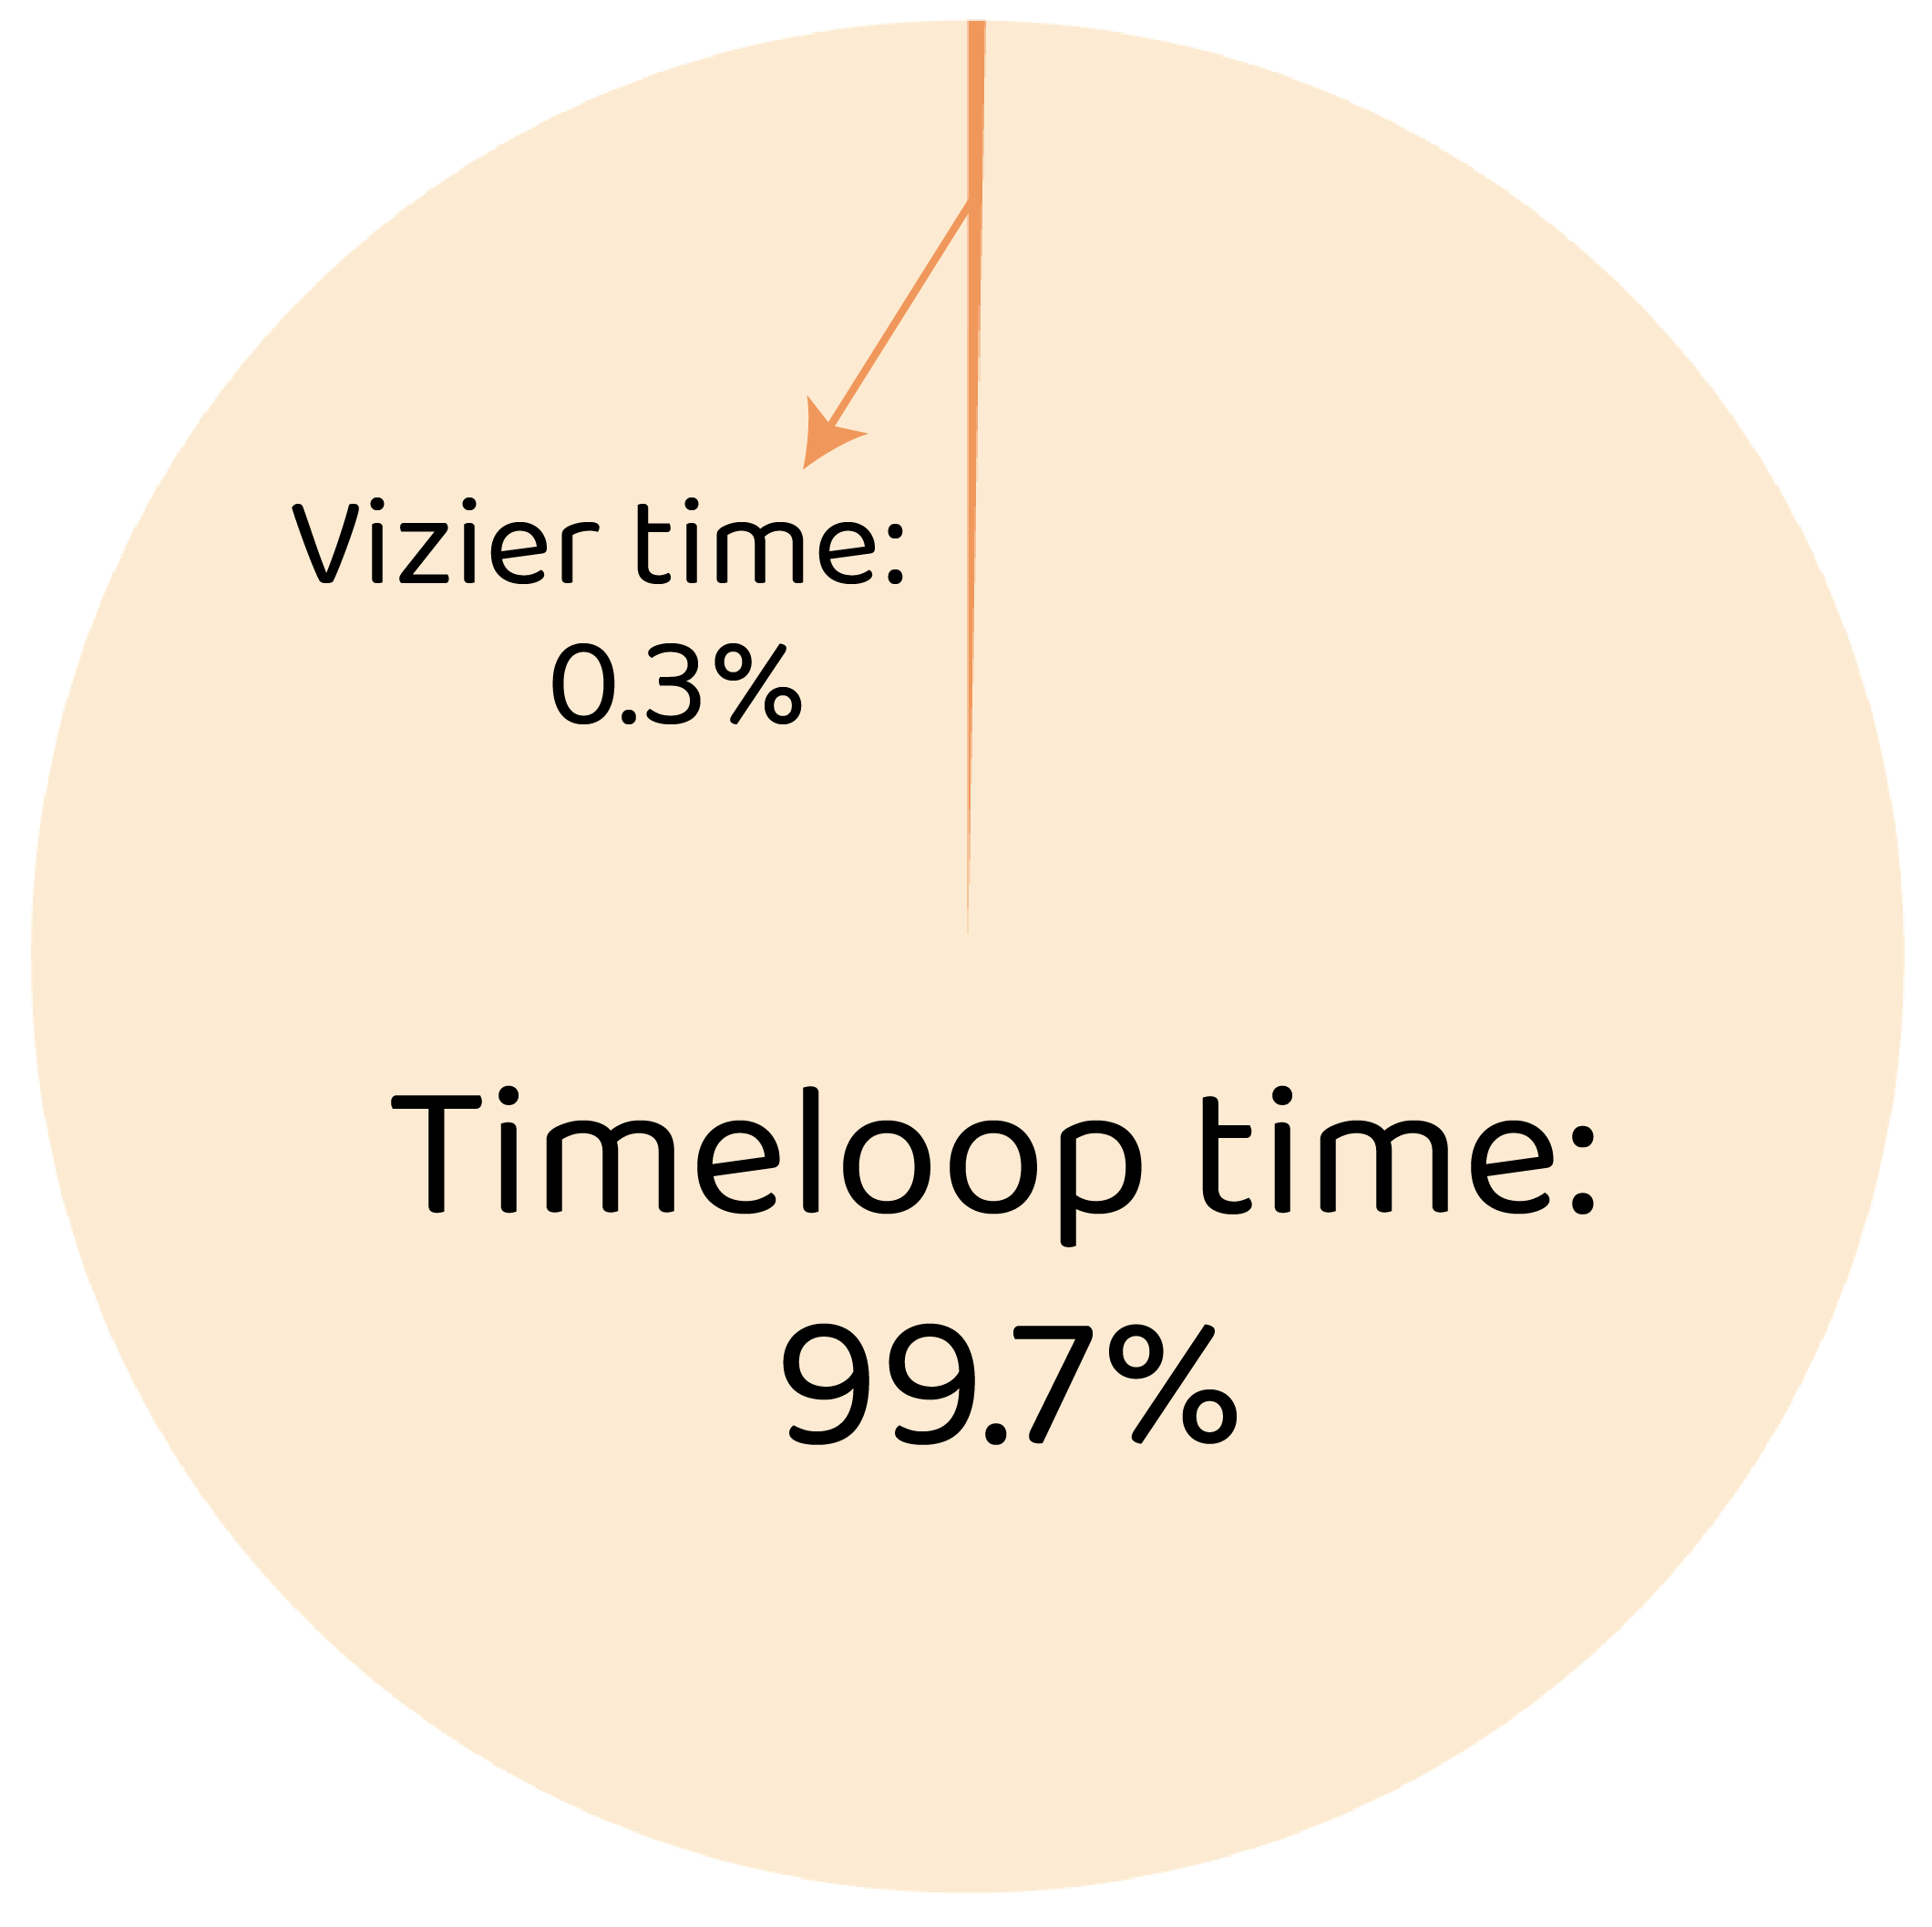
\includegraphics[width=\linewidth]{fig3/timeloop_vs_vizier.png}
%     \caption{Per-trial wall-clock breakdown.}
%     \label{fig:timeloop-time}
%     \vspace{-10pt}
% \end{wrapfigure}
% Despite V0's improvements, it inherits the sequential dependence on external tiling tools (e.g., Timeloop) because it lacks a linear expression for non-linear tiling-fusion interactions. As shown in Figure~\ref{fig:timeloop-time}, Timeloop accounts for over 99\% of per-trial latency, creating a prohibitive bottleneck for multi-thousand-trial searches. To resolve this, CHEETAH-V1 internalizes tiling by precomputing Pareto-pruned configurations and encoding them as decision variables. This removes Timeloop from the critical path, collapsing each trial to a single Vizier-proposal and LP-solve step. We start with introducing the preprocessing stage below before presenting the full formulation in Section~\ref{sec::v1}.

% % The limitations of prior work is still inherited in the V0 formulation due to the difficulty of expressing non-linear relationships as linear constraints. Therefore tiling decisions $(\Tmax_i, \Tmin_i, t_i^k)$ are fixed constants provided by additional software, such as Timeloop. A natural question is whether this sequential dependence also creates a \emph{runtime} bottleneck. Figure~\ref{fig:timeloop-time} confirms that it does: across different models, Timeloop scheduling on average accounts for over 99\% of per-trial wall-clock time, while the Vizier proposal and fusion ILP together consume less than 1\% on average. Because the outer loop requires thousands of trials to converge, the cumulative cost of repeated Timeloop invocations dominates the total search budget. This observation motivates a key design choice in CHEETAH-V1: rather than calling Timeloop online during each trial, we precompute a Pareto-pruned set of tiling configurations once (Section~\ref{sec:pareto}) and encode the tiling selection as decision variables \emph{inside} the LP. This eliminates Timeloop from the per-trial critical path entirely, reducing each trial to a single Vizier-proposal$\,\to\,$LP-solve step.

% % CHEETAH-V1 captures tiling as a \emph{decision variable} inside the LP, enabling the solver to jointly optimize tiling and fusion. We start with describing our preprocessing stage in Section~\ref{sec:pareto} before presenting the full formulation in Section~\ref{sec::v1}.


% \paragraph{Pareto Pruning Pre-Pass} The raw tiling search space for a $7$-dimensional convolution loop with $3$ memory levels is $\mathcal O(10^7)$ configurations per operation. We reduce this to a tractable Pareto-optimal subset $\mathcal{C}_i$ for each operation $i$ via a pre-pass for (1) L1 feasibility where configurations whose tiled working set exceeds L1 scratchpad capacity $C_{L1}$ are discarded; (2) Pareto optimality where a configuration $c$ is retained only if no other configuration achieves both lower $\Tmax_i(c)$ \emph{and} smaller working-set size in the Global Buffer.

% In practice, Pareto pruning reduces $\mathcal O(10^7)$ raw configurations to $|\mathcal{C}_i| \approx 10^2$ to $10^3$ per operation. Timeloop is run once per (operation, configuration) pair, producing the triple $(\Tmin_i(c), \Tmax_i(c), t_i^k(c))$ for each retained configuration $c \in \mathcal{C}_i$. These are precomputed constants---the LP solver makes no Timeloop calls at solve time.

% \paragraph{Time-invariant Pareto fronts.}
% A key observation is that the Pareto front shape is invariant to memory time: configurations are ranked by compute cycles and working-set bytes, neither of which depends on bandwidth. Changing bandwidth rescales the DRAM access cost $t_i^k(c)$ uniformly. This means the Pareto-pruned configuration sets can be precomputed \emph{once} and reused across all Vizier trials that share the same compute configuration class, amortizing the expensive Timeloop precomputation.

% \subsubsection{The Joint CHEETAH-V1 LP Formulation}\label{sec::v1}

% \paragraph{From fixed constants to decision variables.}
% In static and V0 formulations, Timeloop selects a single tiling per operation externally and passes the results to the LP as fixed constants $\Tmax_i$, $\Tmin_i$, $t_i^k$. The DRAM savings from pinning tensor $k$ of operation $i$ is then simply $t_i^k \cdot p_{i,o(i)}^k$---a constant times a variable, which is already linear. V1 brings this tiling choice \emph{inside} the LP by introducing \textbf{tiling selection variables} $y_{i,c} \in [0,1]$, one per Pareto-optimal configuration $c \in \mathcal{C}_i$ from the pre-pass, with the constraint $\sum_c y_{i,c} = 1$ (exactly one configuration is selected per operation). The Timeloop-precomputed constants $\Tmax_i(c)$, $\Tmin_i(c)$, $t_i^k(c)$ now become \emph{per-configuration coefficients} indexed by $c$. This means the DRAM savings term becomes $t_i^k(c) \cdot y_{i,c} \cdot p_{\text{assoc}(i,k),\, o(i)}$. This is a product of \emph{two} decision variables, which is bilinear and cannot be handled by a convex programming directly.
 
% % \paragraph{Linearization via McCormick envelopes.}
% % We linearize this product exactly via the classical McCormick substitution. Specifically,  we introduce \textbf{auxiliary variables} $w_{i,c,k} := y_{i,c} \cdot p_{\text{assoc}(i,k),\, o(i)}$ that represent the joint effect of selecting tiling $c$ \emph{and} pinning tensor $k$, constrained by:
% % \begin{equation}
% % \label{eq:mccormick}
% % \begin{aligned}
% %     w_{i,c,k} &\leq y_{i,c}, \qquad
% %     w_{i,c,k} \leq p_{\text{assoc}(i,k),\, o(i)} \\
% %     w_{i,c,k} &\geq y_{i,c} + p_{\text{assoc}(i,k),\, o(i)} - 1, \qquad
% %     w_{i,c,k} \geq 0
% % \end{aligned}
% % \end{equation}
% % Since both factors lie in $[0,1]$, these four constraints force $w_{i,c,k} = y_{i,c} \cdot p$ at any integer vertex, requiring no manually tuned constants. Together, $y_{i,c}$ and $w_{i,c,k}$ account for 1.6M of the 2.08M variables in the \Vone~ LP (Table~\ref{tab:v1_scale}). \todo{change to MoE?}

% \paragraph{Linearization via McCormick envelopes.}
% We linearize this product exactly via the classical McCormick substitution \citep{mccormick1976computability}. Specifically, we introduce \textbf{auxiliary variables} $w_{i,c,k} := y_{i,c} \cdot p_{\text{assoc}(i,k),\, o(i)}$ that represent the joint effect of selecting tiling $c$ \emph{and} pinning tensor $k$, constrained by:
% \begin{equation}
% \label{eq:mccormick}
% \begin{aligned}
%     w_{i,c,k} &\leq y_{i,c}, \qquad
%     w_{i,c,k} \leq p_{\text{assoc}(i,k),\, o(i)} \\
%     w_{i,c,k} &\geq y_{i,c} + p_{\text{assoc}(i,k),\, o(i)} - 1, \qquad
%     w_{i,c,k} \geq 0
% \end{aligned}
% \end{equation}
% Since both factors lie in $[0,1]$, these four constraints force $w_{i,c,k} = y_{i,c} \cdot p$ at any integer vertex, requiring no manually tuned constants. Together, $y_{i,c}$ and $w_{i,c,k}$ constitute the majority of V1's decision variables (Table~\ref{tab:v1_scale}).
 

% % \paragraph{Full formulation.}
% % Combining tiling selection, time-indexed placement, rematerialization, and McCormick linearization, the full V1  formulation is:

% % \begin{equation}
% % % \label{eq:v1}
% % \begin{aligned}
% % \min \quad & \sum_{i \in \mathcal{N}} T_i + \sum_{i \in \mathcal{N}} \sum_{t \in \mathcal{T}} c_i^{\text{remat}} \, r_{i,t} \\[4pt]
% % \text{s.t.} \quad
% % & \sum_{c \in \mathcal{C}_i} y_{i,c} = 1 & \forall\, i \in \mathcal{N} \\[3pt]
% % & T_i \geq \sum_{c \in \mathcal{C}_i} \Tmax_i(c)\, y_{i,c} - \sum_{c \in \mathcal{C}_i} \sum_{k} t_i^k(c)\, w_{i,c,k} & \forall\, i \in \mathcal{N} \\[3pt]
% % & T_i \geq \sum_{c \in \mathcal{C}_i} \Tmin_i(c)\, y_{i,c} & \forall\, i \in \mathcal{N} \\[3pt]
% % & w_{i,c,k} \leq y_{i,c} & \forall\, i, c, k \\
% % & w_{i,c,k} \leq p_{\text{assoc}(i,k),\, o(i)} & \forall\, i, c, k \\
% % & w_{i,c,k} \geq y_{i,c} + p_{\text{assoc}(i,k),\, o(i)} - 1 & \forall\, i, c, k \\[3pt]
% % & \sum_{e \in \mathcal{E}} d_e\, p_{e,t} + \sum_{i \in \mathcal{N}} d_i^W\, p_{i,t}^W \leq \CGM & \forall\, t \in \mathcal{T} \\[3pt]
% % & p_{e,t} \leq p_{e,t-1} + r_{\text{src}(e),\, t} & \forall\, e, t > o(\text{src}(e)) \\
% % & p_{i,t}^W \leq p_{i,t-1}^W & \forall\, i, t > o(i) \\[3pt]
% % & r_{i,t} = 0 & \forall\, i, t \leq o(i) \\
% % & r_{i,t} \leq p_{e,t} & \forall\, e \in \text{in}(i), t > o(i) \\
% % & r_{i,t} \leq p_{i,t}^W & \forall\, i, t > o(i) \\[3pt]
% % & T_i, p_{e,t}, p_{i,t}^W, r_{i,t}, w_{i,c,k} \geq 0 &
% % \end{aligned}
% % \tag{\textcolor{skyblue}{V1}}\label{eq:v1}
% % \end{equation}
% % full formulation below in appendix 
% % \begin{equation}
% % \begin{aligned}
% % \min \quad & \sum_{i \in \mathcal{N}} T_i + \sum_{i \in \mathcal{N}} \sum_{t \in \mathcal{T}} c_i^{\text{remat}} \, r_{i,t} \\[4pt]
% % \text{s.t.} \quad
% % & \sum_{c \in \mathcal{C}_i} y_{i,c} = 1 & \forall\, i \in \mathcal{N} \\[3pt]
% % & T_i \geq \max\!\left(\sum_{c \in \mathcal{C}_i} \Tmin_i(c)\, y_{i,c},\;\; \sum_{c \in \mathcal{C}_i} \Tmax_i(c)\, y_{i,c} - \sum_{c \in \mathcal{C}_i} \sum_{k} t_i^k(c)\, w_{i,c,k}\right) & \forall\, i \in \mathcal{N} \\[3pt]
% % & w_{i,c,k} \leq y_{i,c}, \quad w_{i,c,k} \leq p_{\text{assoc}(i,k),\, o(i)}, \quad w_{i,c,k} \geq y_{i,c} + p_{\text{assoc}(i,k),\, o(i)} - 1 & \forall\, i, c, k \\[3pt]
% % & \sum_{e \in \mathcal{E}} d_e\, p_{e,t} + \sum_{i \in \mathcal{N}} d_i^W\, p_{i,t}^W \leq \CGM & \forall\, t \in \mathcal{T} \\[3pt]
% % & p_{e,t} \leq p_{e,t-1} + r_{\text{src}(e),\, t} & \forall\, e,\, t > o(\text{src}(e)) \\
% % & p_{i,t}^W \leq p_{i,t-1}^W & \forall\, i,\, t > o(i) \\[3pt]
% % & r_{i,t} = 0 \;\; \forall\, t \leq o(i); \quad r_{i,t} \leq \min\!\big(p_{e,t},\, p_{i,t}^W\big) \;\; \forall\, e \in \text{in}(i),\, t > o(i) \\[3pt]
% % & T_i,\, p_{e,t},\, p_{i,t}^W,\, r_{i,t},\, w_{i,c,k} \geq 0 &
% % \end{aligned}
% % \tag{\textcolor{skyblue}{V1}}\label{eq:v1}
% % \end{equation}

% \paragraph{Variable and constraint digest.}
% The V1 formulation inherits all the features of the V0 formulation, and additionally captures tiling by introducing selection variables
% $y_{i,c} \in [0,1]$, constrained by $\sum_c y_{i,c} = 1$, to choose
% from $|\mathcal{C}_i|$ Pareto-optimal configurations.
% Each configuration defines compute costs $T_i^{\max}(c)$,
% $T_i^{\min}(c)$, and per-tensor DRAM savings $t_i^k(c)$.
% We linearize the resulting bilinear DRAM-savings term exactly via
% McCormick auxiliary variables $w_{i,c,k}$, which enforce $w_{i,c,k} \;=\; y_{i,c} \cdot p_{\mathrm{assoc}(i,k),\,o(i)}$ at integer vertices without a relaxation gap.

% Per-operation latency $T_i$ is lower-bounded by the weighted
% configuration floor $\sum_c T_i^{\min}(c)\, y_{i,c}$ and the weighted
% off-chip cost $\sum_c T_i^{\max}(c)\, y_{i,c}$ minus achievable savings
% $\sum_{c,k} t_i^k(c)\, w_{i,c,k}$.
% This coupling enables the solver to accept sub-optimal local tiling
% (higher $T_i^{\max}$) if its smaller memory footprint unlocks global
% fusion gains that outweigh the compute-utilization loss.
% Capacity and persistence constraints carry over from V0, utilizing
% edge-indexed placement $p_{e,t}$ to handle multi-fanout nodes.
% For DeepSeek-V3, the V1 LP scales to approximately $2{,}504{,}019$ variables, $2{,}983{,}450$ constraints, and $6{,}094{,}156$ non-zeros. Table~\ref{tab:v1_scale} provides a representative breakdown, Table~\ref{tab:comparison} summarizes features of each more powerful formulation; full per-model sizes are in Table~\ref{tab:exp1_lp_sizes} and \ref{tab:exp2_cluster_lp_sizes}. 



% % The V1 formulation extends V0 by making the tiling configuration a decision variable. The selection variables $y_{i,c} \in [0,1]$, with $\sum_c y_{i,c} = 1$, choose among $|\mathcal{C}_i|$ Pareto-optimal tiling configurations precomputed by Timeloop (Section~\ref{sec:pareto}). Each configuration $c$ determines the operation's compute cost $T_i^{\max}(c)$, on-chip floor $T_i^{\min}(c)$, and per-tensor DRAM savings $t_i^k(c)$.
% % The DRAM savings term $t_i^k(c) \cdot y_{i,c} \cdot p_{\text{assoc}(i,k),\,o(i)}$ 
% % is bilinear in the tiling selection and placement variables; we linearize it 
% % via McCormick auxiliary variables $w_{i,c,k}$, constrained by 
% % $w_{i,c,k} \leq y_{i,c}$, $w_{i,c,k} \leq p_{\text{assoc}(i,k),\,o(i)}$, and 
% % $w_{i,c,k} \geq y_{i,c} + p_{\text{assoc}(i,k),\,o(i)} - 1$. 
% % These three inequalities force $w_{i,c,k} = y_{i,c} \cdot p_{\text{assoc}(i,k),\,o(i)}$ 
% % at any integer-feasible point (\cref{prop:mccormick_exact}), so the LP exactly captures the 
% % bilinear interaction without introducing any relaxation gap at integer vertices.
% % The $T_i$ lower bound now takes the maximum of two configuration-dependent terms: the weighted on-chip floor $\sum_c T_i^{\min}(c)\, y_{i,c}$ and the weighted off-chip cost minus achievable savings $\sum_c T_i^{\max}(c)\, y_{i,c} - \sum_{c,k} t_i^k(c)\, w_{i,c,k}$.
% % This coupling is the core novelty of V1: the solver can accept a tiling with higher $T_i^{\max}(c)$ (lower compute utilization) if its smaller working set enables pinning decisions that reduce total DRAM traffic by more than the utilization loss.
% % All remaining constraints---memory capacity, persistence, and rematerialization---carry over from V0 with edge-indexed placement variables $p_{e,t}$ replacing per-tensor $p_{i,t}^k$ to correctly handle skip connections and multi-fanout nodes. For our largest workload, DeepSeek-V3 ($L \approx 6{,}300$ operations), the V1 LP contains approximately 2.5M variables, 3.0M constraints, and 6.1M nonzeros. Table~\ref{tab:v1_scale} provides a representative breakdown; full per-model sizes are in Table~\ref{tab:v1_scale}. 
% % \paragraph{Key constraint interactions.}
% % The execution-time constraints (lines 2--3: the upper and lower bounds for $T_i$) capture the central trade-off that is unique to \Vone: the LP must commit to a tiling configuration $c$ (via $y_{i,c}$) that sets both the baseline compute cost $\Tmax_i(c)$ and the achievable DRAM savings $t_i^k(c)$. A configuration with smaller tiles may have higher $\Tmax_i(c)$ (lower compute utilization) but smaller working sets, enabling more aggressive pinning. The LP balances these trade-offs simultaneously---precisely the cross-stage interaction that the sequential pipeline cannot discover.
 
% % The edge-indexed persistence constraint (line 8: $p_{e,t} \leq p_{e,t-1} + r_{\text{src}(e),\, t}$) and the memory capacity constraint (line 7: lower bound on $\CGM$) are inherited from \Vzero, which introduced per-edge placement variables $p_{e,t}$ to correctly model skip connections. \Vone~ extends this by coupling edge sizes to the tiling selection---since different configurations $c$ produce different activation working sets, the LP can now jointly reason about how tiling choices affect memory pressure across skip connections.


% \begin{figure}[ht!]
% \begin{minipage}[t]{0.48\textwidth}
% \vspace{0pt}
% \centering
% \captionof{table}{V1 variable and constraint counts
% (representative, DeepSeek-V3).}
% \label{tab:v1_scale}
% \footnotesize
% \begin{tabular}{@{}ll@{}}
% \toprule
% \textbf{Variable} & \textbf{Role} \\
% \midrule
% $T_i$       & Per-operation execution time \\
% $y_{i,c}$   & Tiling config selection ($|\mathcal{C}_i|$ options) \\
% $p_{e,t}$   & Edge-indexed activation placement \\
% $p_{i,t}^W$ & Weight placement \\
% $r_{i,t}$   & Rematerialization indicator \\
% $w_{i,c,k}$ & McCormick auxiliaries ($y_{i,c} \cdot p$) \\
% % \midrule
% % \multicolumn{2}{@{}l}{\textbf{DeepSeek-V3 totals}
% %                        ($L \approx 6{,}300$)} \\
% % \midrule
% % Variables   & $2{,}504{,}019$ \\
% % Constraints & $2{,}983{,}450$ \\
% % Nonzeros    & $6{,}094{,}156$ \\
% \bottomrule
% \end{tabular}
% \end{minipage}%
% \hspace{0.02\textwidth}%
% \begin{minipage}[t]{0.48\textwidth}
% \vspace{0pt}
% \centering
% \captionof{table}{Comparison of static, V0, and V1 formulations.}
% \label{tab:comparison}
% \footnotesize
% \begin{tabular}{@{}lccc@{}}
% \toprule
% \textbf{Property} & \textbf{Static} & \textbf{V0} & \textbf{V1} \\
% \midrule
% Joint tiling + fusion    & $\times$ & $\times$   & \checkmark \\
% Time-indexed placement   & $\times$ & \checkmark & \checkmark \\
% Rematerialization        & $\times$ & \checkmark & \checkmark \\
% Relaxed skip connections & $\times$ & Partial    & \checkmark \\
% \bottomrule
% \end{tabular}

% \medskip
% \raggedright
% \footnotesize
% % \textbf{Comparison across formulations.}
% % Table~\ref{tab:comparison} summarizes the progression from the
% % static formulation through V0 to V1.
% \end{minipage}
% \end{figure}


% % \begin{table}[ht!]
% % \centering
% % \caption{V1 variable and constraint counts (representative, DeepSeek-V3).}
% % \label{tab:v1_scale}
% % \small
% % \begin{tabular}{lrl}
% % \toprule
% % \textbf{Variable} & \textbf{Role} \\
% % \midrule
% % $T_i$ & Per-operation execution time \\
% % $y_{i,c}$ & Tiling configuration selection ($|\mathcal{C}_i|$ options per op) \\
% % $p_{e,t}$ & Edge-indexed activation placement \\
% % $p_{i,t}^W$ & Weight placement \\
% % $r_{i,t}$ & Rematerialization indicator \\
% % $w_{i,c,k}$ & McCormick auxiliaries ($y_{i,c} \cdot p$) \\
% % \midrule
% % \multicolumn{2}{l}{\textbf{DeepSeek-V3 totals} ($L \approx 6{,}300$)} \\
% % \midrule
% % Variables & 2,504,019 \\
% % Constraints & 2,983,450 \\
% % Nonzeros & 6,094,156 \\
% % \bottomrule
% % \end{tabular}
% % \end{table}
% % \paragraph{Comparison across formulations.}
% % Table~\ref{tab:comparison} summarizes the progression from static through V0 to V1.
% % \begin{table}[ht!]
% % \centering
% % \caption{Comparison of static, V0, and V1 formulations.}
% % \label{tab:comparison}
% % \small
% % \begin{tabular}{lccc}
% % \toprule
% % \textbf{Property} & \textbf{static} & \textbf{V0} & \textbf{V1} \\
% % \midrule
% % Joint tiling + fusion & \texttimes & \texttimes & \checkmark \\
% % Time-indexed placement & \texttimes & \checkmark & \checkmark \\
% % Rematerialization & \texttimes & \checkmark & \checkmark \\
% % Relaxed skip connections & \texttimes & Partial & \checkmark \\
% % % Config-dependent DRAM savings & \texttimes & \texttimes & \checkmark \\ 
% % % Bilinear linearization & --- & --- & McCormick \\
% % \bottomrule
% % \end{tabular}
% % \end{table}

% % \paragraph{Structural invariance for efficient LLM integration.}
% % A practical advantage of both our LP formulations is that the constraint matrix sparsity pattern is invariant across hardware configurations---only the numerical coefficients change. This means:
% % \begin{itemize}
% %     \item The LP solver's preconditioner can be designed once per neural network model and reused across all Vizier trials.
% %     \item An LLM-Architect can reason about constraint structure (which constraints are binding, which variables are fractional) without needing to understand the full LP.
% %     \item Warm-starting from a previous trial's LP solution is straightforward since the variable indexing is stable.
% % \end{itemize}

% \subsection{Strategic Intelligence: LLM-Guided Outer Search}
% \label{sec:llm_outer}
% We use Google Vizier as a black-box Bayesian optimizer to propose hardware configurations. While effective, vanilla Vizier treats search as pure function optimization, often requiring thousands of iterations to identify suboptimal regions without leveraging structural hardware-workload knowledge. To address this, we introduce an LLM-guided outer-loop controller based on SkyDiscovery that reasons about co-design decisions. By learning from a causal ledger of past trials and Lagrangian dual signals from the LP solver, the LLM proposes meaningful, constrained search-space candidates. This integration is enabled by the CHEETAH-V1 formulation, which removes the Timeloop bottleneck to reduce trial times from days to hours.The LLM-Architect reduces wasted trials by intelligently steering Vizier’s search without altering the inner solver or its optimality certificates. In this hybrid loop, the LLM determines global architectural regions, Vizier performs local Bayesian optimization within those patches, and the large-scale V1 LP solver evaluates each concrete candidate. The LLM-Architect loop proceeds as follows: 
% % We use Vizier as a black-box Bayesian optimizer to propose candidate hardware configurations. While effective, Vizier search strategies (LCS, UCB, etc) requires thousands of iterations explore and learn which regions are suboptimal and treats the search as a pure function optimization problem without leveraging structural knowledge about hardware-workload interactions.
% % We leverage an LLM-guided outer-loop controller that learns from logs of thousands of past co-design trials to propose meaningful search-space candidates for Vizier. This is a SkyDiscovery based outer LLM layer which reasons about hardware-software co-design decisions and learns from a causal ledger of constantly updated logs across trials, as well as feed-back signal such as dual variables through the LP solve. This is possible for CHEETAH-V1 LP formulation, since it removes the Timeloop-in-the-loop constraint, thus reducing the co-design problem from days to hours, and permitting the LLM outer loop. 

% % The LLM-Architect does not change the inner solver, and retains all the optimal certificates of the V1 LP formulation, but intelligently changes where the Vizier outer hardware optimizer searches to reduce wasted trials. The LLM proposes global decisions to determine constrained regions of the hardware search space; Vizier then performs local Bayesian optimization inside those regions; which then passes downstream into a large scale LP solver for the V1 formulation to evaluate each concrete candidate. The LLM-Architect loop proceeds as follows:

% \begin{enumerate}[leftmargin=1.6em, itemsep=4pt]

% \item \textbf{Extraction.}
% Deterministic scripts summarize recent trials into a \emph{Causal
% Ledger}. Each record includes hardware parameters, validity, Perf/TDP,
% LP cycles, capacity duals/slacks, bandwidth sensitivity, MFU, memory
% utilization, roofline gap, failure class, and LP solver metrics.

% \item \textbf{Context building.}
% The last $N$ trials and the Causal Ledger are compressed into a compact
% JSON context for the Architect. The context emphasizes empirical
% feasibility, observed invalid regions, best known valid designs, and
% physical audit signals.

% \item \textbf{Architect.}
% The online Architect, implemented as Qwen2.5-7B-Instruct with a LoRA
% adapter trained on past trial logs, diagnoses the dominant bottleneck
% and emits a campaign patch. The patch constrains macro-architectural
% search decisions such as Global Memory, DRAM bandwidth, total MACs,
% systolic shape, PE grid, and batch size. A larger teacher model,
% DeepSeek-V3.2, was used offline to generate or critique campaign labels
% but is not in the live loop.

% \item \textbf{Campaign validation.}
% A deterministic validator clips or rejects the LLM patch to enforce
% legal hardware ranges, TDP and area limits, MAC caps, CGM feasibility
% floors, compute/bandwidth coupling, and roofline constraints. This
% prevents the LLM from proposing physically implausible regions such as
% maximum-MAC/minimum-bandwidth designs.

% \item \textbf{Local optimization.}
% Vizier is initialized inside the validated patch and warm-started with
% prior trials that lie in the same region. Vizier then samples concrete
% hardware candidates within the approved campaign. The LLM therefore
% chooses the high-level architectural neighbourhood, while Vizier
% performs local adaptive optimization.

% \item \textbf{Unified V1 evaluation.}
% The large-scale LP solver evaluates each candidate by solving the V1
% joint tiling-fusion-placement LP using saved Pareto $\mathcal{C}$-sets.
% It returns the objective, cycles, selected tiling configurations,
% placement/rematerialization decisions, dual/slack summaries, and
% solver-quality diagnostics.

% \item \textbf{Roofline audit.}
% A deterministic Roofline Auditor checks whether the predicted latency
% is physically plausible. For each candidate we compute
% \begin{align}
%     t_{\text{compute}} &=
%         \frac{\text{useful FLOPs}}{\text{peak FLOPs/s}},
%     \qquad
%     t_{\text{memory}}  =
%         \frac{\text{post-placement DRAM bytes}}{\text{peak bandwidth}},
%     \nonumber\\
%     t_{\text{ideal}}   &=
%         \max\!\left(t_{\text{compute}},\, t_{\text{memory}}\right).
%     \label{eq:roofline_audit}
% \end{align}
% A candidate is rejected if the solver-reported latency falls below this
% lower bound, or if MFU or memory utilization exceeds 1.0 within
% tolerance.

% \item \textbf{Ledger update.}
% The loop records the campaign hypothesis, intervention, observed
% invalid-rate change, MFU change, roofline validity, and best Perf/TDP
% change. The ledger also records forbidden regions when a campaign
% produces excessive invalid trials.

% \end{enumerate}

% \noindent The Architect receives workload summaries, invalid-rate
% history, MFU, roofline signals, prior valid regions, normalized LP duals,
% and bandwidth sensitivities. The system starts from a safe empirically
% valid patch and permits duals only to make bounded edits, such as raising
% the CGM floor, increasing bandwidth, reducing MAC count, or changing
% systolic shapes. The validator rejects any dual-guided patch that
% excludes known high-performing valid regions or predicts a substantially
% worse feasible rate. This provides controlled architectural feedback in
% addition to prompt input.


% % \todo{Expand this section once the LLM+RL experimental protocol is finalized. Key questions to address: (1) Which LLM is used and how is it prompted? (2) How are LLM proposals integrated with Vizier's Bayesian model? (3) What is the sample efficiency improvement over pure Vizier?}





% edit for page limit 
\section{Methodology}
\label{sec:methods}
We present the \textbf{CHEETAH} (\acroletter{C}o-designed \acroletter{H}ardware \acroletter{E}xploration via \acroletter{E}fficient \acroletter{T}hroughput and \acroletter{H}ybrid-search) framework in three parts: Section~\ref{sec:v0} introduces CHEETAH-V0, which extends the static fusion ILP with time-indexed placement and rematerialization. Section~\ref{sec:v1} presents CHEETAH-V1, which jointly optimizes tiling and fusion via McCormick linearization. Section~\ref{sec:llm_outer} describes the LLM-Architect outer loop. Appendix~\ref{sec:theory} provides theoretical analysis on the exactness of our mathematical modeling, and Appendix~\ref{app:invar} provides details on structured constraint matrices, and Appendix~\ref{app:llm_loop} presents the LLM Architect outer loop design details.

\paragraph{What the program optimizes over: static structure, dynamic dimensions.}
A single model's compute graph is \emph{structurally static}: the layers and
dependencies of, say, Llama-70B do not change from request to request. What
varies at inference is the \emph{data and the dimensions}: sequence length, batch
size, mixture-of-experts routing, and the number of decode steps. CHEETAH is
therefore a \emph{design-time} program, solved offline over the static structure
at a representative operating point (context, batch, generation length) together
with workload statistics (per-expert routing frequency $f_e$, the prefix
cache-hit profile). The chip is designed once for the operating envelope, not
re-solved per request. Data-dependent routing enters as a distribution: the
expected number of distinct experts touched at the deployed batch (a
balls-in-bins occupancy model), with load-balancing and token-drop caps bounding
the tail. When a deployment spans a wide range of shapes, the same program is
solved over a distribution of operating points (a few weighted
$(\text{context},\text{batch},\text{routing})$ samples) to yield a design robust
across the dynamic range rather than overfit to one point; such a stochastic
objective is the weighted sum $\sum_k w_k T^{(k)}$ over the samples, and the
robust one the epigraph $T \ge T^{(k)}$ for every sample; both are linear rows
of the same LP. Per-request scheduling of one realized dynamic graph is
a separate problem (a fixed-hardware compiler), not the co-design program studied
here.


% \subsection{\Vzero~: Multi-Period Placement with Rematerialization}
\subsection{CHEETAH-V0: Multi-Period Placement with Rematerialization}
\label{sec:v0}

Our first extension models the neural network's (NN) execution as a sequence of $T$ discrete timesteps (one per operation in execution order). This decides at which time, which tensor is pinned, evicted, or recomputed to optimally minimize cycle counts. The key features are:

\paragraph{Time-indexed placement.}
Instead of a single binary $p_i^k$ per tensor, we introduce $p_{i,t}^k \in [0,1]$ for each tensor $k$ of layer $i$ at each timestep $t$. A tensor can be pinned at timestep $t=5$, and evicted at $t=10$. This models a dynamic memory manager within a single inference pass.

\paragraph{Rematerialization.}
Rather than always paying DRAM bandwidth to reload an evicted tensor, we introduce variables $r_{i,t} \in [0,1]$ indicating that layer $i$ is recomputed at timestep $t$ to restore its output to the Global Buffer. This is particularly valuable for models such as EfficientNet, where depthwise convolutions account for only ${\sim}5\%$ of total FLOPs but produce large activation tensors. Recomputing a depthwise layer to avoid re-reading 6\,MiB from DRAM at 256\,GB/s can be faster than the DRAM reload itself.

\paragraph{Relaxed skip-connection handling.}
CHEETAH-V0 lifts the baseline's restriction to consecutive operations by using edge-indexed placement variables $p_{e,t}$ for each edge $e \in \mathcal{E}$, correctly modeling multi-fanout skip connections where consumers independently benefit from on-chip data.

The CHEETAH-V0 LP formulation is:
\begin{equation}
% \label{eq:v0}
\begin{aligned}
\min \quad & \sum_{i \in \mathcal{N}} T_i + \sum_{i \in \mathcal{N}} \sum_{t \in \mathcal{T}} c_i^{\text{remat}} \, r_{i,t} \\
\text{s.t.} \quad
& T_i \geq \Tmax_i - \sum_{k \in \{I,O,W\}} t_i^k \cdot p_{i,o(i)}^k & \forall\, i \in \mathcal{N} \\
& T_i \geq \Tmin_i & \forall\, i \in \mathcal{N} \\
& \sum_{i \in \mathcal{N}} \sum_{k} d_i^k \, p_{i,t}^k \leq \CGM & \forall\, t \in \mathcal{T} \\
& p_{i,t}^k \leq p_{i,t-1}^k + r_{i,t} & \forall\, i, t, k \in \{I,O\} \\
& p_{i,t}^W \leq p_{i,t-1}^W & \forall\, i, t \\
& r_{i,t} = 0 & \forall\, i, t \leq o(i) \\
& 0 \leq p_{i,t}^k, r_{i,t} \leq 1 &
\end{aligned}
\tag{V0}\label{eq:v0}
\end{equation}


where $o(i)$ is the execution order of operation $i$, $d_i^k$ is the byte size of tensor $k$ for layer $i$, and $c_i^{\text{remat}}$ is the recomputation cost.

\paragraph{Variable and constraint digest.}
The objective minimizes total execution time $\sum_i T_i$ plus rematerialization costs. Per-operation latency $T_i$ is lower-bounded by the on-chip floor $T_i^{\min}$ and the off-chip time $T_i^{\max}$ adjusted for DRAM savings from pinned tensors. Persistence constraints enforce monotone eviction for weights and allow recomputation-based restoration for activations; rematerialization is only permitted post-execution and requires on-chip availability of both inputs and weights.
For DeepSeek-V3 ($L \approx 6{,}300$), this formulation yields a large-scale program with approximately 3.3M variables and 3.7M constraints. See Appendix~\ref{sec:lps} for a detailed breakdown. 


% \subsection{\textcolor{skyblue}{V1}: Joint Tiling and Fusion via McCormick Linearization}
% \vspace{-6pt}
\subsection{CHEETAH-V1: Joint Tiling, Fusion, and Hardware Sizing Inside the Program}
\label{sec:v1}

\begin{wrapfigure}{r}{0.2\linewidth}
    % \vspace{-12pt}
    \centering
    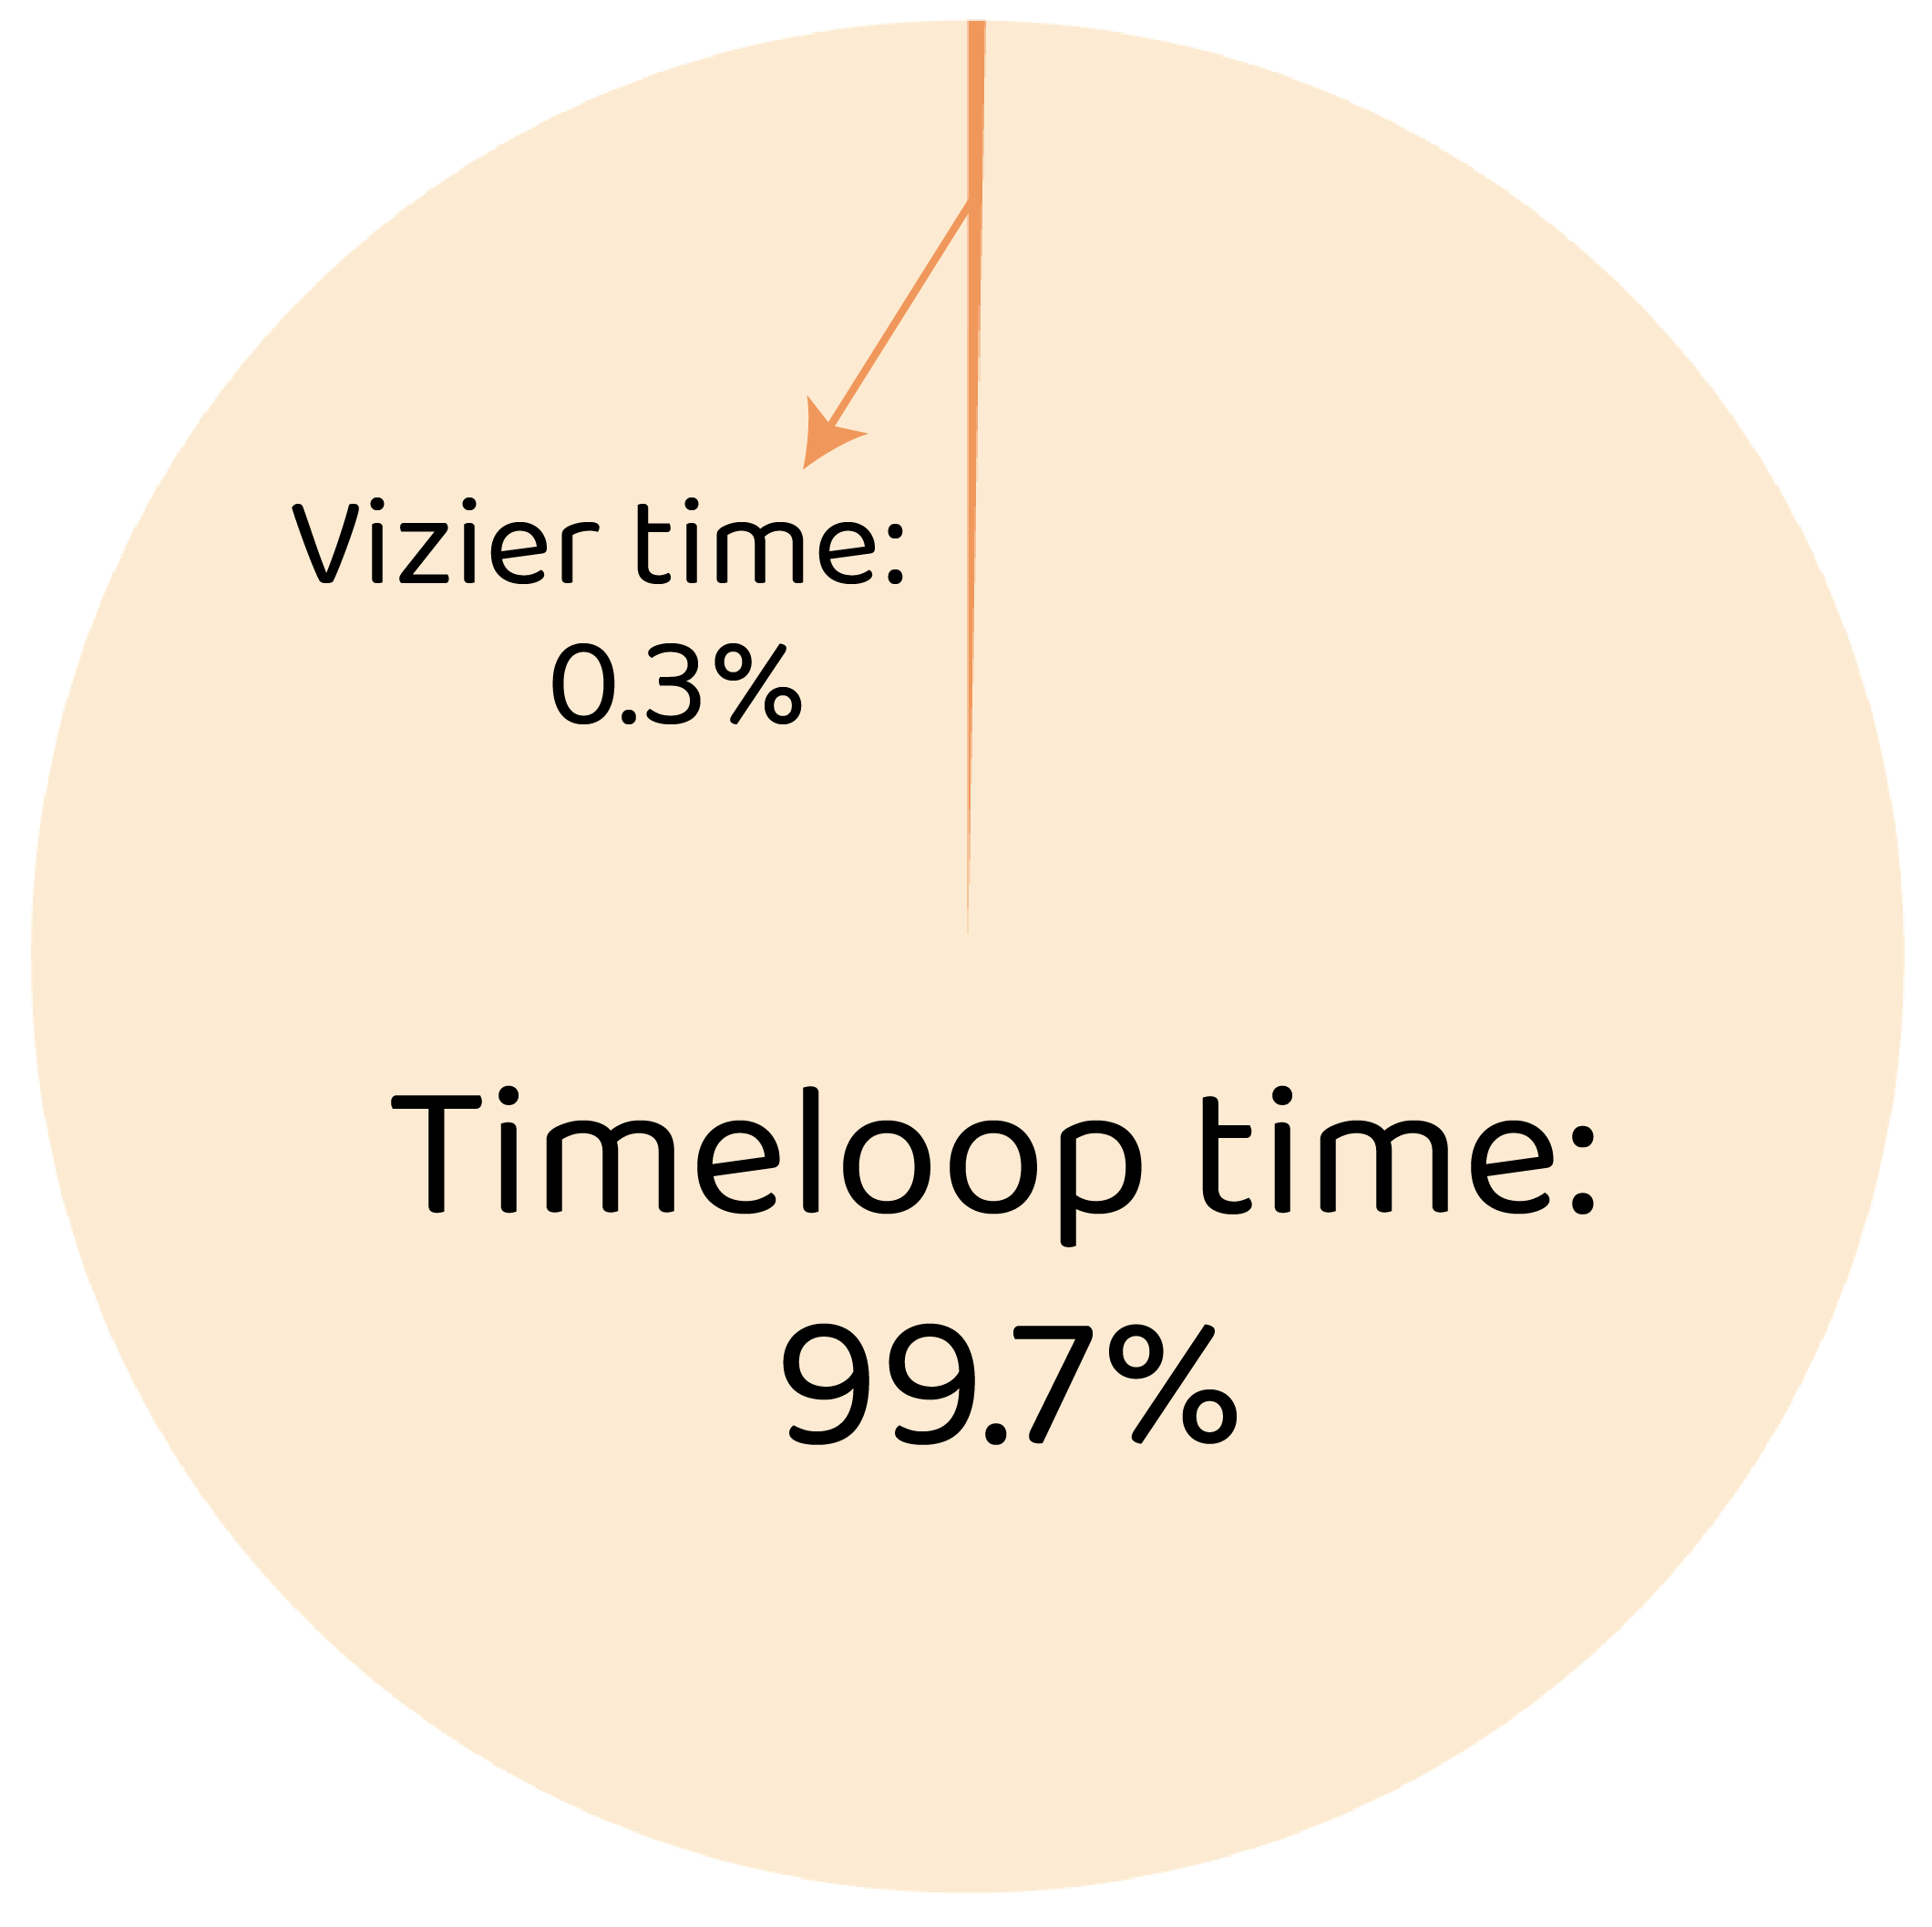
\includegraphics[width=\linewidth]{fig3/timeloop_vs_vizier.png}
    \caption{Per-trial wall-clock breakdown.}
    \label{fig:timeloop-time}
    % \vspace{-10pt}
\end{wrapfigure}
Despite V0's improvements, it inherits the sequential dependence on external tiling tools (e.g., Timeloop) because it lacks a linear expression for non-linear tiling-fusion interactions. As shown in Figure~\ref{fig:timeloop-time}, Timeloop accounts for over 99\% of per-trial latency, creating a prohibitive bottleneck for multi-thousand-trial searches. To resolve this, CHEETAH-V1 internalizes tiling by precomputing Pareto-pruned configurations and encoding them as decision variables. This removes Timeloop from the critical path, collapsing each trial to a single Vizier-proposal and LP-solve step. We start with introducing the preprocessing stage below before presenting the full formulation.

% The limitations of prior work is still inherited in the V0 formulation due to the difficulty of expressing non-linear relationships as linear constraints. Therefore tiling decisions $(\Tmax_i, \Tmin_i, t_i^k)$ are fixed constants provided by additional software, such as Timeloop. A natural question is whether this sequential dependence also creates a \emph{runtime} bottleneck. Figure~\ref{fig:timeloop-time} confirms that it does: across different models, Timeloop scheduling on average accounts for over 99\% of per-trial wall-clock time, while the Vizier proposal and fusion ILP together consume less than 1\% on average. Because the outer loop requires thousands of trials to converge, the cumulative cost of repeated Timeloop invocations dominates the total search budget. This observation motivates a key design choice in CHEETAH-V1: rather than calling Timeloop online during each trial, we precompute a Pareto-pruned set of tiling configurations once (Section~\ref{sec:pareto}) and encode the tiling selection as decision variables \emph{inside} the LP. This eliminates Timeloop from the per-trial critical path entirely, reducing each trial to a single Vizier-proposal$\,\to\,$LP-solve step.

% CHEETAH-V1 captures tiling as a \emph{decision variable} inside the LP, enabling the solver to jointly optimize tiling and fusion. We start with describing our preprocessing stage in Section~\ref{sec:pareto} before presenting the full formulation in Section~\ref{sec::v1}.


\paragraph{Pareto pruning pre-pass.} The raw tiling search space for a $7$-dimensional convolution loop with $3$ memory levels is $\mathcal O(10^7)$ configurations per operation. We reduce this to a tractable Pareto-optimal subset $\mathcal{C}_i$ for each operation $i$ via a pre-pass for (1) L1 feasibility where configurations whose tiled working set exceeds L1 scratchpad capacity $C_{L1}$ are discarded; (2) Pareto optimality where a configuration $c$ is retained only if no other configuration achieves both lower $\Tmax_i(c)$ \emph{and} smaller working-set size in the Global Buffer.

In practice, Pareto pruning reduces $\mathcal O(10^7)$ raw configurations to $|\mathcal{C}_i| \approx 10^2$ to $10^3$ per operation. Timeloop is run once per (operation, configuration) pair, producing the triple $(\Tmin_i(c), \Tmax_i(c), t_i^k(c))$ for each retained configuration $c \in \mathcal{C}_i$. These are precomputed constants: the LP solver makes no Timeloop calls at solve time. Appendix~\ref{app:details} provides more details.

\paragraph{Time-invariant Pareto fronts.}
A key observation is that the Pareto front shape is invariant to memory time: configurations are ranked by compute cycles and working-set bytes, neither of which depends on bandwidth. Changing bandwidth rescales the DRAM access cost $t_i^k(c)$ uniformly. This means the Pareto-pruned configuration sets can be precomputed \emph{once} and reused across all Vizier trials that share the same compute configuration class, amortizing the expensive Timeloop precomputation.

% \subsubsection{The Joint CHEETAH-V1 LP Formulation}\label{sec::v1}

\paragraph{From fixed constants to decision variables.}
V1 brings the tiling choice \emph{inside} the LP by introducing \textbf{tiling selection variables} $y_{i,c} \in [0,1]$, one per Pareto-optimal configuration $c \in \mathcal{C}_i$ from the pre-pass, with the constraint $\sum_c y_{i,c} = 1$ (exactly one configuration is selected per operation). The Timeloop-precomputed constants $\Tmax_i(c)$, $\Tmin_i(c)$, $t_i^k(c)$ now become \emph{per-configuration coefficients} indexed by $c$, so the DRAM savings term becomes $t_i^k(c) \cdot y_{i,c} \cdot p_{\text{assoc}(i,k),\, o(i)}$, a bilinear product that we linearize below.
 
% \paragraph{Linearization via McCormick envelopes.}
% We linearize this product exactly via the classical McCormick substitution. Specifically,  we introduce \textbf{auxiliary variables} $w_{i,c,k} := y_{i,c} \cdot p_{\text{assoc}(i,k),\, o(i)}$ that represent the joint effect of selecting tiling $c$ \emph{and} pinning tensor $k$, constrained by:
% \begin{equation}
% \label{eq:mccormick}
% \begin{aligned}
%     w_{i,c,k} &\leq y_{i,c}, \qquad
%     w_{i,c,k} \leq p_{\text{assoc}(i,k),\, o(i)} \\
%     w_{i,c,k} &\geq y_{i,c} + p_{\text{assoc}(i,k),\, o(i)} - 1, \qquad
%     w_{i,c,k} \geq 0
% \end{aligned}
% \end{equation}
% Since both factors lie in $[0,1]$, these four constraints force $w_{i,c,k} = y_{i,c} \cdot p$ at any integer vertex, requiring no manually tuned constants. Together, $y_{i,c}$ and $w_{i,c,k}$ account for 1.6M of the 2.08M variables in the \Vone~ LP (Table~\ref{tab:v1_scale}). \todo{change to MoE?}

\paragraph{Linearization via McCormick envelopes.}
We linearize this product exactly via the classical McCormick substitution \citep{mccormick1976computability}. For a bilinear term whose factors live in the unit box, the McCormick system is not merely \emph{a} linear relaxation but the convex hull of the product's graph $\{(y,p,w) : w = y\,p,\ 0 \le y,p \le 1\}$: no tighter linear description exists without lifting to additional variables, and it is exact whenever either factor is integral. Relaxation looseness can therefore enter only through fractional $(y,p)$ pairs, a quantity our rounding-and-replay audits measure per workload.
Specifically, we introduce \textbf{auxiliary variables} $w_{i,c,k} := y_{i,c} \cdot p_{\text{assoc}(i,k),\, o(i)}$ that represent the joint effect of selecting tiling $c$ \emph{and} pinning tensor $k$, constrained by:
% \vspace{-4pt}
\begin{equation}
\label{eq:mccormick}
\begin{aligned}
    w_{i,c,k} &\leq y_{i,c}, \qquad
    w_{i,c,k} \leq p_{\text{assoc}(i,k),\, o(i)} \\
    w_{i,c,k} &\geq y_{i,c} + p_{\text{assoc}(i,k),\, o(i)} - 1, \qquad
    w_{i,c,k} \geq 0
\end{aligned}
\end{equation}
Since both factors lie in $[0,1]$, these four constraints force $w_{i,c,k} = y_{i,c} \cdot p$ at any integer vertex, requiring no manually tuned constants.
Geometrically (Figure~\ref{fig:mccormick}), the two upper inequalities are the concave envelope of the bilinear term $w = y\,p$ over the unit box and the two lower ones its convex envelope: the tightest concave over-estimator and convex under-estimator of the product. Because the product is bilinear over a box, these envelopes coincide with the convex hull and are exact at the integer corners, so an integral tile choice is credited with exactly its true DRAM savings, whereas a fractional blend of tiles can be over-credited by up to one quarter of the savings coefficient (at $y = p = \tfrac12$). This over-credit is one of the two mechanisms behind the relaxation gap in V1 and V2, the other being the aggregate roofline row that Section~\ref{sec:v1} disaggregates, and it is exactly what the rounding-and-replay audits measure. Together, $y_{i,c}$ and $w_{i,c,k}$ constitute the majority of V1's decision variables (Table~\ref{tab:v1_scale}).

\begin{figure}[h!]
\centering
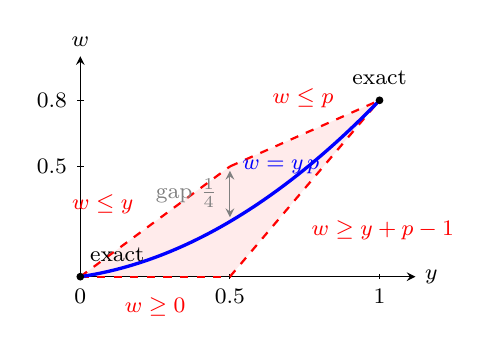
\begin{tikzpicture}[x=3.8cm, y=2.8cm, >=stealth, font=\footnotesize]
  % feasible McCormick region on the slice p = 0.2 + 0.6y: a kite with 4 distinct edges
  \fill[red!8] (0,0) -- (0.5,0.5) -- (1,0.8) -- (0.5,0) -- cycle;
  \draw[->] (0,0) -- (1.12,0) node[right] {$y$};
  \draw[->] (0,0) -- (0,1.0) node[above] {$w$};
  \foreach \t in {0,0.5,1} { \draw (\t,0.012) -- (\t,-0.012) node[below] {$\t$}; }
  \foreach \t in {0.5,0.8} { \draw (0.012,\t) -- (-0.012,\t) node[left] {$\t$}; }
  % upper pair: w <= y (slope 1) and w <= p = 0.2 + 0.6y
  \draw[red, dashed, thick] (0,0) -- (0.5,0.5);
  \draw[red, dashed, thick] (0.5,0.5) -- (1,0.8);
  \node[red, above left] at (0.21,0.24) {$w \le y$};
  \node[red, above left, xshift=2pt] at (0.86,0.72) {$w \le p$};
  % lower pair: w >= 0 and w >= y + p - 1 = 1.6y - 0.8
  \draw[red, dashed, thick] (0,0) -- (0.5,0);
  \draw[red, dashed, thick] (0.5,0) -- (1,0.8);
  \node[red, below] at (0.25,-0.05) {$w \ge 0$};
  \node[red, below right] at (0.74,0.30) {$w \ge y + p - 1$};
  % true product along the slice: w = y(0.2 + 0.6y)
  \draw[blue, very thick, domain=0:1, samples=60, smooth] plot (\x, {\x*(0.2+0.6*\x)});
  \node[blue] at (0.67,0.50) {$w = y\,p$};
  % maximal gap at y = p = 1/2
  \draw[<->, gray] (0.5,0.27) -- (0.5,0.48);
  \node[gray, left] at (0.49,0.38) {gap $\tfrac14$};
  % exact at the integer corners
  \fill (0,0) circle (1.4pt);
  \fill (1,0.8) circle (1.4pt);
  \node[above right, yshift=2pt] at (0,0) {exact};
  \node[above, yshift=2pt] at (1,0.8) {exact};
\end{tikzpicture}
\caption{McCormick envelope of the bilinear term $w = y\,p$ on the unit box, drawn along the slice $p = 0.2 + 0.6\,y$ so that all four inequalities of \eqref{eq:mccormick} are distinct lines: the upper pair $w \le y$, $w \le p$ forms the roof and the lower pair $w \ge 0$, $w \ge y + p - 1$ the floor of the shaded feasible region, and the true product (blue) lies inside, touching the envelope only at the integer corners $y \in \{0,1\}$. The largest over-credit is $\tfrac14$, attained at $y = p = \tfrac12$.}
\label{fig:mccormick}
\end{figure}
% \vspace{-4pt}
\paragraph{The Joint CHEETAH-V1 LP Formulation.}
Combining tiling selection, time-indexed placement, rematerialization, and McCormick linearization yields the full V1 program. We do not display it separately: it is the special case of the flagship program \eqref{eq:v1} with the hardware reciprocals $v,u$ pinned to the proposed chip, the CGM one-hot $h_{\mathrm{GM}}$ pinned to its memory, and the tile-dependent families $z^{\mathrm{act}}, z^{W}$ dropped; it in turn contains the fixed-chip program \eqref{eq:v0}, and \eqref{eq:v1} is displayed in full at the end of Section~\ref{sec:v1}.

\paragraph{Tile-dependent residency.}
Extending V1's linearization, V2 introduces two additional McCormick families
for the bilinear products that couple tile choice to on-chip residency:
\begin{equation}
\label{eq:mccormick_v2}
\begin{aligned}
z^{\mathrm{act}}_{e,c,t} \equiv y_{\mathrm{dst}(e),c}\, p_{e,t}: \quad
& z^{\mathrm{act}}_{e,c,t} \leq y_{\mathrm{dst}(e),c}, \quad
  z^{\mathrm{act}}_{e,c,t} \leq p_{e,t}, \\
& z^{\mathrm{act}}_{e,c,t} \geq y_{\mathrm{dst}(e),c} + p_{e,t} - 1, \quad
  z^{\mathrm{act}}_{e,c,t} \geq 0, \\[3pt]
z^{W}_{i,c,t} \equiv y_{i,c}\, p^{W}_{i,t}: \quad
& z^{W}_{i,c,t} \leq y_{i,c}, \quad
  z^{W}_{i,c,t} \leq p^{W}_{i,t}, \\
& z^{W}_{i,c,t} \geq y_{i,c} + p^{W}_{i,t} - 1, \quad
  z^{W}_{i,c,t} \geq 0.
\end{aligned}
\end{equation}
V2 also promotes the CGM size itself to an LP decision.  Let $\{2^k \text{ MiB}
: k = 0, \ldots, K-1\}$ be a discrete size grid and $h_{\mathrm{GM},k} \in [0,1]$
a one-hot selector; the chip's on-chip global-buffer capacity is then
$\sum_{k} 2^{k}\, h_{\mathrm{GM},k}$ bytes.
% \vspace{-4pt}

\paragraph{Hardware sizing inside the same program.}\label{sec:v3}
The rows above optimize the schedule for a \emph{fixed} chip proposed by the
outer loop. CHEETAH-V1 closes the final decoupling in the same program: it
promotes the chip's compute and bandwidth to LP decisions and replaces the
aggregate roofline with its exact convex hull. Fixing the hardware knobs and
collapsing the disaggregated variables recovers the fixed-chip case exactly, so
this single formulation subsumes CHEETAH-V0 and is our flagship program.

\paragraph{Hardware as decision variables.}
Alongside the one-hot CGM selector $h_{\mathrm{GM},k}$, the flagship program
\eqref{eq:v1} sizes the MAC array
and DRAM bandwidth \emph{inside} the program. Writing the reference-normalized
reciprocals $v = M_{\mathrm{ref}}/\mathrm{MACs}$ and
$u = \mathrm{BW_{ref}}/\mathrm{BW}$ (so a tile's compute time is $\Tmin_i(c)\,v$
and its memory time is $\Tmax_i(c)\,u$), the chip must respect the same-silicon
area and power envelopes
\begin{equation}
\kappa_{\mathrm{MAC}}\,\mathrm{MACs}
 + \kappa_{\mathrm{SRAM}}\!\sum_{k} 2^{k} h_{\mathrm{GM},k}
 + \kappa_{\mathrm{BW}}\,\mathrm{BW} \;\le\; A_{\mathrm{cap}},
\qquad
\pi_{\mathrm{MAC}}\,\mathrm{MACs} \;\le\; P_{\mathrm{cap}} .
\label{eq:v3_caps}
\end{equation}
The reciprocals are convex epigraphs, and the program is a linear program.
Bandwidth \emph{is} a finite menu: $\mathrm{BW}$ is a one-hot selection
$\nu_\ell$ over the gate-feasible legal points $\mathrm{BW}_\ell$
($8$ of the $12$ catalogue points on DeepSeek-V3 pass the pin gate
$\mathrm{BW}/0.8\le 4096$ pins), so
$u=1/\mathrm{BW}=\sum_\ell \nu_\ell/\mathrm{BW}_\ell$ is exact at integral
$\nu$ and the LP relaxation of the menu is a valid lower bound. The compute
reciprocal $v \ge 1/m$ is bracketed by tangent rows on a geometric grid of $m$
(a valid relaxation, hence a certified lower bound) and by chord rows on the
same grid (an inner approximation); with 89 grid rows each envelope is within
$10^{-3}$ of $1/m$, so the bracket is at most $2\times10^{-3}$ wide, and no
auxiliary variable is needed. Every product of a
menu selector with a continuous quantity is written as its convex hull
(disaggregated copies with a linking equality), which is exact at integral
selectors; McCormick envelopes are used only in that hull form. The chord
(inner) LP yields an achievable design only once every menu selector is pinned
to an integral value and the pinned solution passes an exact-lift check
(reciprocals and products set to their true values, every original row
re-verified); with relaxed selectors it is neither a lower nor an upper bound,
so every ``exact'' below means exact at integral selectors. This internalizes the hardware proposal the outer loop previously
made, so a single solve sizes chip \emph{and} schedule jointly under a hard
area/TDP budget.

\paragraph{Disaggregated perspective epigraph.}
The aggregate roofline row
$T_i \ge \max\!\big(\sum_c \Tmin_i(c)\,y_{i,c}\,v,\; \sum_c (\Tmax_i(c){-}\mathrm{save})\,y_{i,c}\,u\big)$,
the form used before the per-tile split below,
is loose once $y$ is fractional: it lets the solver blend a compute-bound tile
against a bandwidth-bound tile and hide \emph{both} bottlenecks
(the source of a large relaxation gap on weight-heavy models). The flagship
program \eqref{eq:v1} replaces it
with the disaggregated perspective form
\begin{equation}
\begin{aligned}
&\textstyle\sum_c v_{i,c}=v,\quad \sum_c u_{i,c}=u;\qquad
 \underline v\,y_{i,c}\le v_{i,c}\le \overline v\,y_{i,c},\quad
 \underline u\,y_{i,c}\le u_{i,c}\le \overline u\,y_{i,c};\\[2pt]
&\tau_{i,c}\ge \Tmin_i(c)\,v_{i,c},\quad
 \tau_{i,c}\ge \big(\Tmax_i(c)-\mathrm{save}_{i,c}\big)\,u_{i,c},\quad
 T_i\ge \textstyle\sum_c \tau_{i,c},
\end{aligned}
\label{eq:v3_epigraph}
\end{equation}
which is the closed convex hull of the per-op ``pick one tile, pay its roofline
maximum'' disjunction: it enforces $T_i \ge \sum_c \max(\cdot,\cdot)$ rather than
the weaker $\max(\sum,\sum)$, tightening the certified lower bound at no cost to
feasibility and preserving exactness at every integer vertex.

\paragraph{Certified column generation.}
The Pareto tile set $\mathcal C_i$ is a column \emph{pool}: a candidate
tiling/mapping enters only when its reduced cost against the converged LP dual
variables is negative. The native mapper (or the LLM-Architect outer loop,
which reads exactly these Lagrangian duals) can therefore \emph{propose}
columns while the LP \emph{scores and certifies} them. The oracle can reshape
where the search looks; it can never weaken the optimality certificate. This is
the mechanism that makes ``the LLM proposes, the solver certifies'' rigorous,
and it is what the outer loop of the next subsection exploits.

\paragraph{The joint CHEETAH-V1 LP formulation.}
Collecting the pieces, the full V1 program takes the fixed-chip rows above with the aggregate
roofline row replaced by the disaggregated perspective epigraph, the reciprocals
$v,u$ and the memory one-hot promoted to decisions under the same-silicon caps,
and one further hull family $X_{i,c,\ell}$, the bandwidth-menu copies of the
memory-time numerator $X_{i,c}=\Tmax_i(c)\,y_{i,c}-\sum_k t_i^k(c)\,w_{i,c,k}$,
so that the DRAM savings scale with bandwidth exactly at integral $\nu$. Writing $m = \mathrm{MACs}/M_{\mathrm{ref}}$ and
$\beta = \mathrm{BW}/\mathrm{BW_{ref}}$, the program is \eqref{eq:v1}.
The CHEETAH-V1 LP formulation is:
\begin{equation}
\begin{aligned}
\min \quad & \sum_{i \in \mathcal{N}} T_i \;+\;
             \sum_{i \in \mathcal{N}} \sum_{t \in \mathcal{T}} c_i^{\text{remat}}\, r_{i,t}
             \;+\; \varepsilon_{\mathrm{CGM}} \sum_{k=0}^{K-1} k \, h_{\mathrm{GM},k} \\[3pt]
\text{s.t.} \quad
& \sum_{c \in \mathcal{C}_i} y_{i,c} = 1 \;\;\forall\, i, \qquad
  \sum_{k=0}^{K-1} h_{\mathrm{GM},k} = 1 \\[3pt]
& v \;\geq\; \tfrac{2}{m_j} - \tfrac{m}{m_j^{2}} \quad \forall\, j \in \mathcal{J}
  \quad\text{(tangent rows; chord rows for the inner LP)} \\[3pt]
& \beta = \textstyle\sum_{\ell} \nu_\ell\, \beta_\ell, \qquad
  u = \textstyle\sum_{\ell} \nu_\ell/\beta_\ell, \qquad
  \textstyle\sum_{\ell} \nu_\ell = 1 \quad\text{(bandwidth menu)} \\[3pt]
& \kappa_{\mathrm{MAC}}\,\mathrm{MACs} + \kappa_{\mathrm{SRAM}}\!\sum_{k} 2^{k} h_{\mathrm{GM},k}
  + \kappa_{\mathrm{BW}}\,\mathrm{BW} \leq A_{\mathrm{cap}}, \qquad
  \pi_{\mathrm{MAC}}\,\mathrm{MACs} \leq P_{\mathrm{cap}} \\[3pt]
& \sum_{c \in \mathcal{C}_i} v_{i,c} = v, \qquad \sum_{c \in \mathcal{C}_i} u_{i,c} = u
  \quad \forall\, i \\[3pt]
& \underline v\, y_{i,c} \leq v_{i,c} \leq \overline v\, y_{i,c}, \qquad
  \underline u\, y_{i,c} \leq u_{i,c} \leq \overline u\, y_{i,c}
  \quad \forall\, i, c \\[3pt]
& \tau_{i,c} \geq \Tmin_i(c)\, v_{i,c}, \qquad
  \tau_{i,c} \geq \textstyle\sum_{\ell} X_{i,c,\ell}/\beta_\ell, \qquad
  T_i \geq \sum_{c \in \mathcal{C}_i} \tau_{i,c} \quad \forall\, i, c \\[3pt]
& \text{Envelopes~\eqref{eq:mccormick} for } w_{i,c,k};\;
  X_{i,c} = \Tmax_i(c)\,y_{i,c} - \textstyle\sum_k t_i^k(c)\,w_{i,c,k} = \textstyle\sum_{\ell} X_{i,c,\ell}
  \quad \forall\, i, c \\[3pt]
& \underline X_{i,c}\,\nu_\ell \le X_{i,c,\ell} \le \Tmax_i(c)\,\nu_\ell
  \quad \forall\, i, c, \ell \\[3pt]
& 
  \text{\eqref{eq:mccormick_v2} for } z^{\mathrm{act}}_{e,c,t}, z^{W}_{i,c,t} \\[3pt]
& \sum_{e \in \mathcal{E}_{\mathrm{live}}(t)} \sum_{c}
    d^{\mathrm{act}}_{e,c}\, z^{\mathrm{act}}_{e,c,t}
  + \sum_{i} \sum_{c} d^{W}_{i,c}\, z^{W}_{i,c,t}
  \leq \sum_{k=0}^{K-1} 2^{k}\, h_{\mathrm{GM},k}
  \quad \forall\, t \\[3pt]
& p_{e,t} \leq p_{e,t-1} + r_{\text{src}(e),\, t} \;\;\forall\, e,\, t > o(\text{src}(e)); \qquad
  p_{i,t}^W \leq p_{i,t-1}^W \;\;\forall\, i,\, t > o(i) \\[3pt]
& r_{i,t} = 0 \;\;\forall\, t \leq o(i); \qquad
  r_{i,t} \leq \min\!\big(p_{e,t},\, p_{i,t}^W\big)
  \;\;\forall\, e \in \text{in}(i),\, t > o(i) \\[3pt]
& T_i,\, \tau_{i,c},\, v_{i,c},\, u_{i,c} \geq 0; \quad
  y, p, p^W, r, w, z, h_{\mathrm{GM}}, \nu \in [0,1]; \quad
  v \in [\underline v, \overline v],\; u \in [\underline u, \overline u]
\end{aligned}
\tag{V1}\label{eq:v1}
\end{equation}

Here $\underline X_{i,c}=\min\{0,\,\Tmax_i(c)-\sum_k t_i^k(c)\}$: in the
measured tile caches the per-tensor byte terms can exceed $\Tmax_i(c)$, so the
numerator box is not sign-restricted, and the bandwidth-menu rows
($X_{i,c,\ell}$, $\nu_\ell$) are exact at integral $\nu$.
Pinning $(v,u,h_{\mathrm{GM}})$ to a proposed chip makes the cap, tangent, and
link rows inert, turns the menu copies $X_{i,c,\ell}$ into the constant multiple
$X_{i,c}/\beta$, and leaves
\eqref{eq:v1} up to the tightening of Corollary~\ref{cor:v3_hull}; this is the
precise sense in which the flagship program subsumes V0. When an achievable
certified sub-problem is required, the compute tangent rows are replaced by the
chord rows with every menu selector pinned (the inner LP), whose solution is a
design once the exact-lift check passes; bandwidth is already a menu and needs no
replacement. This is the form used by the column-generation oracle.

\subsection{The Comprehensive CHEETAH-V1: Serving-Regime Co-Design Decisions}\label{sec:v3_levers}
Program~\eqref{eq:v1} sizes compute, bandwidth, and on-chip memory jointly with
the schedule. The memory-bound decode regime of LLM, MoE, and diffusion serving
admits four further decisions, each of which reduces the bytes moved or sets a
hardware capacity, hence is a linear (or McCormick-linearizable) addition to
the flagship program \eqref{eq:v1} rather than an outer-loop guess. We fold them in below. Every added block is
\emph{inert when pinned}: fixing its selector to a baseline policy leaves
\eqref{eq:v1}, and with it the V0 and V1 chain, exactly intact, so the subsumption
property is preserved. Decisions that only rescale coefficients (the decode batch
$N$, the speculative-decode width $K$) enter as workload parameters that reshape
the per-op dimensions and thus arithmetic intensity, and the flagship program
\eqref{eq:v1} evaluates any $(N,K)$ without deciding them; genuinely discrete or non-convex choices (draft
model, eviction policy, denoising-step schedule) remain columns the outer loop
proposes and the LP evaluates against its duals. Accuracy is never linearized: each
precision menu below is restricted to configurations the quantization literature
certifies as lossless-enough.

\paragraph{Precision as a decision (per phase, per expert).}
Let $\mathcal{Q}$ be an accuracy-vetted precision menu, each point $\rho$
carrying weight-, activation-, and KV-bit fractions $(b^W_\rho,b^A_\rho,
b^{\mathrm{KV}}_\rho)$ relative to the 8-bit baseline. We write a menu entry as
$\mathrm{W}w\mathrm{A}a$, meaning $w$-bit weights and $a$-bit activations, with a
trailing $/\mathrm{KV}k$ when the KV cache is additionally held at $k$ bits. The
menu used here is
\[
  \rho \in \{\;
  \underbrace{\mathrm{W8A8}}_{\text{8-bit weights, 8-bit activations}},\;
  \underbrace{\mathrm{W4A8}}_{\text{4-bit weights, 8-bit activations}},\;
  \underbrace{\mathrm{W4A8/KV4}}_{\text{as W4A8, plus a 4-bit KV cache}},\;
  \underbrace{\mathrm{W4A16}}_{\text{4-bit weights, 16-bit activations}}
  \;\},
\]
each admissible under AWQ, GPTQ and KVQuant
\citep{lin2024awq,frantar2023gptq,hooper2024kvquant}. Narrower weights reduce the
bytes a decode step must stream, which is the dominant cost; narrower activations
additionally reduce multiplier switching energy, and \cref{sec:energy_coeff}
reports the measured saving for each entry. Per phase
$\phi \in \{\mathrm{pre},\mathrm{dec}\}$ a one-hot selector chooses the operating
precision, inducing byte-scales:
\begin{equation}
\sum_{\rho} q_{\phi,\rho} = 1,\qquad
s^{W}_\phi = \sum_\rho b^W_\rho\, q_{\phi,\rho},\qquad
s^{\mathrm{KV}}_\phi = \sum_\rho b^{\mathrm{KV}}_\rho\, q_{\phi,\rho},\qquad
q_{\phi,\rho}\in\{0,1\}.
\label{eq:v3_prec}
\end{equation}
The weight and KV byte footprints $d^{W}_{i,c}$ and $d^{\mathrm{KV}}$ in the
capacity row and the DRAM-savings term are replaced by $s^{W}_{\phi}d^{W}_{i,c}$
and $s^{\mathrm{KV}}_{\phi}d^{\mathrm{KV}}$; the resulting selector-times-variable
products are written as hull disaggregations of the per-step byte aggregates
over the precision menu (exact at integral $q$). For a mixture-of-experts layer the phase index is
refined to an \emph{expert} index: each expert $e$ carries its own one-hot
$q_{e,\rho}$ and byte-scale $s^{W}_e=\sum_\rho b^W_\rho q_{e,\rho}$, so the solver
may place the lowest-bit points on the hottest experts, where weight-reload
traffic dominates.

\paragraph{Energy-aware same-silicon cap.}
Precision helps under a fixed power budget only if bandwidth actually costs
power, so the cap of~\eqref{eq:v3_caps} is extended to charge DRAM traffic at
$\pi_{\mathrm{bit}}$ joules per bit:
\begin{equation}
\pi_{\mathrm{MAC}}\,\mathrm{MACs} \;+\; \pi_{\mathrm{bit}}\, \varrho_{\mathrm{DRAM}}
\;\le\; P_{\mathrm{cap}},
\qquad
\varrho_{\mathrm{DRAM}} = \sum_{\text{class}\,\in\,\{W,A,\mathrm{KV}\}}
   s^{\text{class}}_{\phi}\,\beta_{\text{class}} ,
\label{eq:v3_power}
\end{equation}
where $\varrho_{\mathrm{DRAM}}$ is the precision-scaled DRAM byte-rate over the
weight, activation, and KV classes; each $\beta_{\text{class}}$ is a workload
constant (the bytes of that class streamed at the reference operating point),
so the row is linear in the precision selectors. Setting $\pi_{\mathrm{bit}}=0$ recovers
\eqref{eq:v3_caps}; a positive $\pi_{\mathrm{bit}}$ is precisely what makes
provisioned bandwidth ``cost power'' in the certified program, so the
byte-reducing decisions (precision, KV budget, expert residency) relax the same cap
that raw bandwidth tightens.

\paragraph{MoE expert residency (HBM pinning).}
Let $C_{\mathrm{HBM}}$ be the fast-memory capacity, a hardware decision entering
the area cap, and let $f_e\in[0,1]$ be expert $e$'s measured routing frequency (a
workload statistic). A pin variable $g_e$ is the resident fraction of expert
$e$'s weights: residency is knapsack-constrained, and an offloaded expert pays a
per-visit reload:
\begin{equation}
\sum_{e} g_e\, s^{W}_e\, W_e \;\le\; C_{\mathrm{HBM}},
\qquad
\Delta^{\mathrm{moe}}_{\mathrm{dram}} = \sum_{e} f_e\,(1-g_e)\, s^{W}_e\, W_e,
\qquad g_e \in [0,1],
\label{eq:v3_expres}
\end{equation}
with $W_e$ the expert weight bytes and $\Delta^{\mathrm{moe}}_{\mathrm{dram}}$ the
expert-reload traffic added to the decode memory term. Pinning the hottest
experts removes their reload; the dual variable $\lambda_{\mathrm{HBM}}$ of the
capacity row is the marginal value of fast memory the outer loop reads when
sizing $C_{\mathrm{HBM}}$.

\paragraph{KV budget (eviction as a resource cap).}
A retained-cache budget $B^{\mathrm{KV}} \in [B_{\min},L_{\mathrm{ctx}}]$ replaces
the growing context length in the attention-input traffic, with $B_{\min}$ the
quality floor of the eviction method (external). With per-token KV footprint
$d^{\mathrm{KV}}$ and an on-chip residency indicator $\sigma_{\mathrm{KV}}\in
\{0,1\}$, the budget is disaggregated over the joint one-hot $\pi_{\rho,s}$ of
decode precision $\rho$ and residency branch $s\in\{\mathrm{on},\mathrm{off}\}$
(with $\sum_{\rho,s}\pi_{\rho,s}=1$, $\sum_s\pi_{\rho,s}=q_{\mathrm{dec},\rho}$,
$\sum_\rho\pi_{\rho,\mathrm{on}}=\sigma_{\mathrm{KV}}$),
\begin{equation}
\begin{aligned}
&B^{\mathrm{KV}}=\textstyle\sum_{\rho,s}B_{\rho,s},\qquad
B_{\min}\,\pi_{\rho,s}\le B_{\rho,s}\le L_{\mathrm{ctx}}\,\pi_{\rho,s},\\[2pt]
&\Delta^{\mathrm{KV}}_{\mathrm{dram}} =
   d^{\mathrm{KV}}\textstyle\sum_\rho b^{\mathrm{KV}}_\rho\, B_{\rho,\mathrm{off}},
\qquad
d^{\mathrm{KV}}\textstyle\sum_\rho b^{\mathrm{KV}}_\rho\, B_{\rho,\mathrm{on}}
   \;\le\; \textstyle\sum_k 2^k h_{\mathrm{GM},k},
\end{aligned}
\label{eq:v3_kvbudget}
\end{equation}
a two-branch hull with no big-$M$, exact at integral $(q,\sigma_{\mathrm{KV}})$,
so that a small enough budget on the on-chip branch ($\sigma_{\mathrm{KV}}=1$)
lets the KV read be served on chip and leave the DRAM term, coupling the
eviction budget directly to CGM sizing through $\lambda_{\mathrm{CGM}}$.

\paragraph{Diffusion cross-step reuse (DeepCache).}
For an $S$-step denoiser, a per-block reuse variable $\chi_b\in[0,1]$ caches block
$b$'s slow-changing feature map across a window of $W$ steps instead of
recomputing it each step:
\begin{equation}
\widehat{\mathrm{cost}}_b = \big(1 - \chi_b(1 - \tfrac1W)\big)\,\mathrm{cost}_b,
\qquad
\sum_b \chi_b\, F_b \;\le\; \textstyle\sum_k 2^k h_{\mathrm{GM},k},
\label{eq:v3_deepcache}
\end{equation}
where $\mathrm{cost}_b$ is block $b$'s per-step compute and feature traffic, $F_b$
its cached-feature footprint, and the window $W$ and cacheable set are workload
statistics. This gives the otherwise fusion-inert diffusion workload a genuine
cross-step memory decision, the temporal analog of the KV cache.

The remaining decisions are drawn from production serving and kernel systems
(vLLM, SGLang, ThunderKittens, TensorRT-LLM); each enriches the \emph{software}
side of the model and, crucially, ties it more tightly to a \emph{hardware} knob,
so the LP models how the chip and the kernel react to one another.

\paragraph{Prefill--decode interleaving.}
Serving co-schedules compute-bound prefill chunks with memory-bound decode steps;
because their bottlenecks are complementary, an interleaved window fills both
rooflines at once. An interleave fraction $\theta\in[0,\theta_{\max}]$ (bounded by
the prefill backlog and a per-token latency SLA) folds prefill into the decode
window, and the additive $T^{\mathrm{pre}}+N\,T^{\mathrm{dec}}$ is replaced by a
mixed-window epigraph,
\begin{equation}
T_{\mathrm{serve}} \ge \theta\,C^{\mathrm{pre}} + N\,C^{\mathrm{dec}},
\qquad
T_{\mathrm{serve}} \ge \theta\,M^{\mathrm{pre}} + N\,M^{\mathrm{dec}},
\label{eq:v3_interleave}
\end{equation}
with $C^{\mathrm{ph}}$ the lifted compute streams (linear in the per-branch
copies of $v$), $M^{\mathrm{ph}}$ the bandwidth-menu memory streams (linear in
the copies $X_{i,c,\ell}$), and $\theta$ a scheduler constant rather than a
decision, so $T_{\mathrm{serve}}\ge\max(\cdot,\cdot)$ over the combined stream and the optimal
$(v,u)$ ratio now tracks the \emph{combined} arithmetic intensity rather than
either phase alone \citep{kwon2023vllm}.

\paragraph{Load-engine vs.\ compute-worker datapath split.}
Following the load/store-vs-compute worker split of tile kernels
\citep{spector2024thunderkittens}, the die is partitioned between MAC units and
data-movement (DMA/async-copy) engines, and the provisioned bandwidth is
realizable only if enough load engines back it. Adding a load-engine throughput
$B_{\mathrm{LD}}$ (area cost $\kappa_{\mathrm{LD}}$) to the area cap,
\begin{equation}
\kappa_{\mathrm{MAC}}\mathrm{MACs} + \kappa_{\mathrm{LD}}B_{\mathrm{LD}}
 + \kappa_{\mathrm{SRAM}}\!\sum_k 2^k h_{\mathrm{GM},k} + \kappa_{\mathrm{BW}}\mathrm{BW}
 \le A_{\mathrm{cap}},
\qquad
\mathrm{BW}_{\mathrm{eff}} \le \mathrm{BW},\;\; \mathrm{BW}_{\mathrm{eff}} \le B_{\mathrm{LD}},
\label{eq:v3_datapath}
\end{equation}
and the perspective reciprocal reads $u=\mathrm{BW_{ref}}/\mathrm{BW_{eff}}$: a
memory-bound decode buys load engines ($\lambda_{\mathrm{LD}}$ large), a
compute-bound prefill buys MACs, a split the solver makes per phase.

\paragraph{Prefix and KV cache reuse (RadixAttention).}
Shared prompt prefixes (system prompts, few-shot exemplars, chat history,
repeated images) let requests reuse cached KV, cutting both prefill compute and
KV traffic \citep{zheng2024sglang,kwon2023vllm}. With a cache capacity
$C_{\mathrm{cache}}$ (a hardware decision in the area cap) and a saturating
hit-rate profile $\eta_s\in[0,1)$ measured under cache-aware
(longest-shared-prefix-first) scheduling for the workload's sharing structure, a
one-hot over cache sizes $s\in\mathcal{S}$ scales the reused terms:
\begin{equation}
\sum_s \rho_s = 1,\quad \eta_{\mathrm{hit}} = \sum_s \eta_s\,\rho_s,\quad
\widehat C^{\mathrm{pre}} = (1-\eta_{\mathrm{hit}})\,C^{\mathrm{pre}},\quad
\widehat M^{\mathrm{pre}} = (1-\eta_{\mathrm{hit}})\,M^{\mathrm{pre}},
\label{eq:v3_radix}
\end{equation}
so the solver trades cache area against the prefill recompute and traffic it
removes. The credit applies to the prefill streams only: the decode KV traffic
$\Delta^{\mathrm{KV}}_{\mathrm{dram}}$ is not credited, because a shared prefix
is re-read at every decode step whether or not it was cached at prefill (the
convention of \cref{sec:decode_decomp}). The $\eta_{\mathrm{hit}}\,C^{\mathrm{pre}}$
and $\eta_{\mathrm{hit}}\,M^{\mathrm{pre}}$ products are exact by disaggregating
the prefill streams over the cache-size menu $\rho_s$; the LP relaxation of that
menu is the chord hypograph of the measured hit-rate curve.

\paragraph{Array shape and native tile granularity.}
Fixing MAC \emph{count} leaves the array \emph{shape} free, and utilization is
acutely shape-dependent (a square array idles on skinny decode GEMVs and
depthwise convs, the very cause of the mapper underutilization behind our
analytic compute floor). A one-hot $\alpha_a$ over aspect ratios / native-MMA
tiles $a\in\mathcal{A}$ ($16{\times}16$, WGMMA, TCGEN05) carries a precomputed
per-op utilization $\eta_{i,a}\in(0,1]$; disaggregating $v_{i,c}$ over $a$ as in
the perspective epigraph,
\begin{equation}
\textstyle\sum_a v^{a}_{i,c} = v_{i,c},\quad
0 \le v^{a}_{i,c} \le \overline v\,\alpha_a,\quad
\tau_{i,c} \ge \sum_a \tfrac{\Tmin_i(c)}{\eta_{i,a}}\, v^{a}_{i,c},
\label{eq:v3_arrayshape}
\end{equation}
which co-designs the array to the workload's matmul shapes and directly serves
LLM/MoE decode GEMVs and EfficientNet depthwise convs
\citep{spector2024thunderkittens}. The lower bound $\underline v\,y_{i,c}\le
v_{i,c}$ lives on the tile selector in \eqref{eq:v3_epigraph} and is inherited
by the copies through the linking sum, not placed on the aspect copies: since
$\sum_a\alpha_a=1$, a positive lower bound on every copy would force
$v_{i,c}\ge\underline v$ on every non-selected tile and make every integral tile
choice infeasible (this was found and fixed in the implementation on
2026-09-20). The DVFS copies $v^{f}_{i,c}$ of \eqref{eq:v3_dvfs} carry the same
one-sided bounds, $\sum_f v^{f}_{i,c}=v_{i,c}$ and $0\le v^{f}_{i,c}\le
\overline v\,\phi_{\mathrm{ph},f}$.

\paragraph{Per-phase clock and voltage (DVFS).}
Compute-bound prefill benefits from a high clock; memory-bound decode does not, so
per-phase frequency is a decision. A per-phase one-hot $\phi_{\mathrm{ph},f}$ over
a frequency menu (throughput scale $\gamma_f$, power factor $\pi_f/\pi_0$) scales
the phase compute time and enters the power cap:
\begin{equation}
\sum_f \phi_{\mathrm{ph},f}=1,\qquad
\tau^{\mathrm{ph}}_{i,c} \ge \sum_f \tfrac{\Tmin_i(c)}{\gamma_f}\,v^{f}_{i,c},\qquad
\pi_{\mathrm{MAC}}\mathrm{MACs}\!\sum_f\!\tfrac{\pi_f}{\pi_0}\phi_{\mathrm{dec},f}
 + \pi_{\mathrm{bit}}\varrho_{\mathrm{DRAM}} \le P_{\mathrm{cap}},
\label{eq:v3_dvfs}
\end{equation}
so the chip runs fast in prefill and slow in decode, freeing power for bandwidth
in the phase where compute is idle (the $\mathrm{MACs}\cdot\phi$ term is the hull
$\mathrm{MACs}=\sum_f \mathrm{MACs}_f$, $M_{\min}\phi_f\le\mathrm{MACs}_f\le
M_{\max}\phi_f$, exact at integral $\phi$).

\paragraph{Constrained and speculative decoding (parameters).}
Constrained decoding over a compressed grammar FSM \citep{zheng2024sglang} and
speculative/draft verification emit $K>1$ tokens per forward pass on deterministic
or accepted spans, raising decode arithmetic intensity toward the compute-bound
regime. Like the batch $N$, the effective width $K$ (and the deterministic or
accepted fraction) is a \emph{workload parameter} the program evaluates, not a
decision; the draft model and grammar remain outer-loop inputs.

\paragraph{The comprehensive program and its constraint signals.}
The comprehensive CHEETAH-V1 program is \eqref{eq:v1} augmented with the
precision, capacity, datapath, and scheduling families
\eqref{eq:v3_prec}--\eqref{eq:v3_dvfs}: the interleaved perspective epigraph now
reads the precision-scaled and cache-reduced bytes, the reload/eviction deltas
$\Delta^{\mathrm{moe}}_{\mathrm{dram}}+\Delta^{\mathrm{KV}}_{\mathrm{dram}}$,
and the shape-, frequency-, and load-engine-dependent compute in place of the
fixed footprints. Because every block is inert under a pinned policy, the
subsumption chain
\eqref{eq:v0}$\subseteq$\eqref{eq:v1}$\subseteq$(comprehensive program) holds by
construction. Its converged duals are exactly the resource-dual vector the
LLM-Architect outer loop consumes: $\lambda_{\mathrm{BW}}$ (large in decode)
values a GB/s, $\lambda_{\mathrm{MAC}}\!\approx\!0$ in decode makes added
multipliers visibly worthless (the anti-gaming property as a certificate, not a
claim), and $\lambda_{\mathrm{HBM}},\lambda_{\mathrm{CGM}},\lambda_{\mathrm{LD}},
\lambda_{\mathrm{cache}}$ value capacity for expert pinning, KV residency, load
engines, and prefix reuse. The outer loop then proposes only the genuinely
discrete and non-convex axes (interconnect radix, HBM-stack count, array aspect
ratio, whether to spend area on low-bit MAC units, draft model, denoising-step
schedule) as columns; the LP evaluates each by reduced cost and the same-silicon
caps make inflation infeasible, so the search is a dual-steered, certified column
generation rather than a blind sweep.

% \begin{equation}
% \begin{aligned}
% \min \quad & \sum_{i \in \mathcal{N}} T_i + \sum_{i \in \mathcal{N}} \sum_{t \in \mathcal{T}} c_i^{\text{remat}} \, r_{i,t} \\[4pt]
% \text{s.t.} \quad
% & \sum_{c \in \mathcal{C}_i} y_{i,c} = 1 & \forall\, i \in \mathcal{N} \\[3pt]
% & T_i \geq \max\!\left(\sum_{c \in \mathcal{C}_i} \Tmin_i(c)\, y_{i,c},\;\; \sum_{c \in \mathcal{C}_i} \Tmax_i(c)\, y_{i,c} - \sum_{c \in \mathcal{C}_i} \sum_{k} t_i^k(c)\, w_{i,c,k}\right) & \forall\, i \in \mathcal{N} \\[3pt]
% & w_{i,c,k} \leq y_{i,c}, \quad w_{i,c,k} \leq p_{\text{assoc}(i,k),\, o(i)}, \quad w_{i,c,k} \geq y_{i,c} + p_{\text{assoc}(i,k),\, o(i)} - 1 & \forall\, i, c, k \\[3pt]
% & \sum_{e \in \mathcal{E}} d_e\, p_{e,t} + \sum_{i \in \mathcal{N}} d_i^W\, p_{i,t}^W \leq \CGM & \forall\, t \in \mathcal{T} \\[3pt]
% & p_{e,t} \leq p_{e,t-1} + r_{\text{src}(e),\, t} & \forall\, e,\, t > o(\text{src}(e)) \\
% & p_{i,t}^W \leq p_{i,t-1}^W & \forall\, i,\, t > o(i) \\[3pt]
% & r_{i,t} = 0 \;\; \forall\, t \leq o(i); \quad r_{i,t} \leq \min\!\big(p_{e,t},\, p_{i,t}^W\big) \;\; \forall\, e \in \text{in}(i),\, t > o(i) \\[3pt]
% & T_i,\, p_{e,t},\, p_{i,t}^W,\, r_{i,t},\, w_{i,c,k} \geq 0 &
% \end{aligned}
% \tag{V1}\label{eq:v1}
% \end{equation}

% \vspace{-4pt}



\paragraph{Variable and constraint digest.}
Each tier of the hierarchy inherits every variable of the tiers before it: V0 contributes latency, residency, and rematerialization; V1 adds tile selection $y_{i,c} \in [0,1]$ (constrained by $\sum_c y_{i,c} = 1$ over $|\mathcal{C}_i|$ Pareto-optimal configurations) with its McCormick products; V2 adds memory sizing and tile-dependent residency products; V3 adds hardware sizing and the disaggregated epigraph. Table~\ref{tab:var_digest} collects the full digest; Appendix~\ref{app:lps} describes variables and constraints in detail.
Each configuration defines compute costs $T_i^{\max}(c)$,
$T_i^{\min}(c)$, and per-tensor DRAM savings $t_i^k(c)$; the resulting bilinear DRAM-savings term is linearized exactly via
McCormick auxiliary variables $w_{i,c,k}$, which enforce $w_{i,c,k} \;=\; y_{i,c} \cdot p_{\mathrm{assoc}(i,k),\,o(i)}$ at integer vertices without a relaxation gap.

\begin{table}[h!]
\centering
\caption{Decision-variable digest for the CHEETAH hierarchy. Each tier inherits all variables of the tiers above it in the table.}
\label{tab:var_digest}
\small
\begin{tabular}{llll}
\toprule
Variable & Index set & Tier & Role \\
\midrule
$T_i$ & op $i$ & V0 & per-operation latency (epigraph value) \\
$p_{e,t}$ & edge $e$, step $t$ & V0 & activation residency in on-chip memory \\
$p^{W}_{i,t}$ & op $i$, step $t$ & V0 & weight residency in on-chip memory \\
$r_{i,t}$ & op $i$, step $t$ & V0 & rematerialization trigger \\
\midrule
$y_{i,c}$ & op $i$, config $c\in\mathcal{C}_i$ & V1 & Pareto tile-config selection, $\sum_c y_{i,c}=1$ \\
$w_{i,c,k}$ & op $i$, config $c$, tensor $k$ & V1 & McCormick product $y_{i,c}\cdot p_{\mathrm{assoc}(i,k),o(i)}$ \\
\midrule
$h_{\mathrm{GM},k}$ & size level $k$ & V1 & one-hot on-chip (CGM) capacity selection \\
$z^{\mathrm{act}}_{e,c,t},\ z^{W}_{i,c,t}$ & edge/op, config, step & V1 & tile-dependent capacity products \\
\midrule
$\mathrm{MACs},\,\mathrm{BW}$ & chip scalars & V1 & compute/BW sizing via reciprocals $v,u$ \eqref{eq:v3_caps} \\
$v_{i,c},\ u_{i,c},\ \tau_{i,c}$ & op $i$, config $c$ & V1 & disaggregated perspective epigraph \eqref{eq:v3_epigraph} \\
$X_{i,c,\ell},\ \nu_\ell$ & op $i$, config $c$, menu point $\ell$ & V1 & bandwidth-menu copies; menu selector \\
\bottomrule
\end{tabular}
\end{table}

Per-operation latency $T_i$ is lower-bounded by the weighted
configuration floor $\sum_c T_i^{\min}(c)\, y_{i,c}$ and the weighted
off-chip cost $\sum_c T_i^{\max}(c)\, y_{i,c}$ minus achievable savings
$\sum_{c,k} t_i^k(c)\, w_{i,c,k}$.
This coupling enables the solver to accept sub-optimal local tiling
(higher $T_i^{\max}$) if its smaller memory footprint unlocks global
fusion gains that outweigh the compute-utilization loss.
Capacity and persistence constraints carry over from V0, utilizing
edge-indexed placement $p_{e,t}$ to handle multi-fanout nodes.
For DeepSeek-V3, the V1 LP scales to approximately 2.5M variables,
3.0M constraints and 6.1M nonzeros. Table~\ref{tab:v1_scale} provides a representative breakdown; full per-model sizes are in Table~\ref{tab:exp1_lp_sizes} and \ref{tab:exp2_cluster_lp_sizes} in \cref{append::lp_size}. 



% The V1 formulation extends V0 by making the tiling configuration a decision variable. The selection variables $y_{i,c} \in [0,1]$, with $\sum_c y_{i,c} = 1$, choose among $|\mathcal{C}_i|$ Pareto-optimal tiling configurations precomputed by Timeloop (Section~\ref{sec:pareto}). Each configuration $c$ determines the operation's compute cost $T_i^{\max}(c)$, on-chip floor $T_i^{\min}(c)$, and per-tensor DRAM savings $t_i^k(c)$.
% The DRAM savings term $t_i^k(c) \cdot y_{i,c} \cdot p_{\text{assoc}(i,k),\,o(i)}$ 
% is bilinear in the tiling selection and placement variables; we linearize it 
% via McCormick auxiliary variables $w_{i,c,k}$, constrained by 
% $w_{i,c,k} \leq y_{i,c}$, $w_{i,c,k} \leq p_{\text{assoc}(i,k),\,o(i)}$, and 
% $w_{i,c,k} \geq y_{i,c} + p_{\text{assoc}(i,k),\,o(i)} - 1$. 
% These three inequalities force $w_{i,c,k} = y_{i,c} \cdot p_{\text{assoc}(i,k),\,o(i)}$ 
% at any integer-feasible point (\cref{prop:mccormick_exact}), so the LP exactly captures the 
% bilinear interaction without introducing any relaxation gap at integer vertices.
% The $T_i$ lower bound now takes the maximum of two configuration-dependent terms: the weighted on-chip floor $\sum_c T_i^{\min}(c)\, y_{i,c}$ and the weighted off-chip cost minus achievable savings $\sum_c T_i^{\max}(c)\, y_{i,c} - \sum_{c,k} t_i^k(c)\, w_{i,c,k}$.
% This coupling is the core novelty of V1: the solver can accept a tiling with higher $T_i^{\max}(c)$ (lower compute utilization) if its smaller working set enables pinning decisions that reduce total DRAM traffic by more than the utilization loss.
% All remaining constraints---memory capacity, persistence, and rematerialization---carry over from V0 with edge-indexed placement variables $p_{e,t}$ replacing per-tensor $p_{i,t}^k$ to correctly handle skip connections and multi-fanout nodes. For our largest workload, DeepSeek-V3 ($L \approx 6{,}300$ operations), the V1 LP contains approximately 2.5M variables, 3.0M constraints, and 6.1M nonzeros. Table~\ref{tab:v1_scale} provides a representative breakdown; full per-model sizes are in Table~\ref{tab:v1_scale}. 
% \paragraph{Key constraint interactions.}
% The execution-time constraints (lines 2--3: the upper and lower bounds for $T_i$) capture the central trade-off that is unique to \Vone: the LP must commit to a tiling configuration $c$ (via $y_{i,c}$) that sets both the baseline compute cost $\Tmax_i(c)$ and the achievable DRAM savings $t_i^k(c)$. A configuration with smaller tiles may have higher $\Tmax_i(c)$ (lower compute utilization) but smaller working sets, enabling more aggressive pinning. The LP balances these trade-offs simultaneously---precisely the cross-stage interaction that the sequential pipeline cannot discover.
 
% The edge-indexed persistence constraint (line 8: $p_{e,t} \leq p_{e,t-1} + r_{\text{src}(e),\, t}$) and the memory capacity constraint (line 7: lower bound on $\CGM$) are inherited from \Vzero, which introduced per-edge placement variables $p_{e,t}$ to correctly model skip connections. \Vone~ extends this by coupling edge sizes to the tiling selection---since different configurations $c$ produce different activation working sets, the LP can now jointly reason about how tiling choices affect memory pressure across skip connections.




% \centering
% \caption{V1 variable and constraint counts (representative, DeepSeek-V3).}
% \label{tab:v1_scale}
% \small
% \begin{tabular}{lrl}
% \toprule
% \textbf{Variable} & \textbf{Role} \\
% \midrule
% $T_i$ & Per-operation execution time \\
% $y_{i,c}$ & Tiling configuration selection ($|\mathcal{C}_i|$ options per op) \\
% $p_{e,t}$ & Edge-indexed activation placement \\
% $p_{i,t}^W$ & Weight placement \\
% $r_{i,t}$ & Rematerialization indicator \\
% $w_{i,c,k}$ & McCormick auxiliaries ($y_{i,c} \cdot p$) \\
% \midrule
% \multicolumn{2}{l}{\textbf{DeepSeek-V3 totals} ($L \approx 6{,}300$)} \\
% \midrule
% Variables & 2,504,019 \\
% Constraints & 2,983,450 \\
% Nonzeros & 6,094,156 \\
% \bottomrule
% \end{tabular}
% \end{table}
% \paragraph{Comparison across formulations.}
% Table~\ref{tab:comparison} summarizes the progression from static through V0 to V1.
% \begin{table}[ht!]
% \centering
% \caption{Comparison of static, V0, and V1 formulations.}
% \label{tab:comparison}
% \small
% \begin{tabular}{lccc}
% \toprule
% \textbf{Property} & \textbf{static} & \textbf{V0} & \textbf{V1} \\
% \midrule
% Joint tiling + fusion & \texttimes & \texttimes & \checkmark \\
% Time-indexed placement & \texttimes & \checkmark & \checkmark \\
% Rematerialization & \texttimes & \checkmark & \checkmark \\
% Relaxed skip connections & \texttimes & Partial & \checkmark \\
% % Config-dependent DRAM savings & \texttimes & \texttimes & \checkmark \\ 
% % Bilinear linearization & --- & --- & McCormick \\
% \bottomrule
% \end{tabular}
% \end{table}

% \paragraph{Structural invariance for efficient LLM integration.}
% A practical advantage of both our LP formulations is that the constraint matrix sparsity pattern is invariant across hardware configurations---only the numerical coefficients change. This means:
% \begin{itemize}
%     \item The LP solver's preconditioner can be designed once per neural network model and reused across all Vizier trials.
%     \item An LLM-Architect can reason about constraint structure (which constraints are binding, which variables are fractional) without needing to understand the full LP.
%     \item Warm-starting from a previous trial's LP solution is straightforward since the variable indexing is stable.
% \end{itemize}

\begin{table}[t]
\centering
\caption{Decision variables of the merged CHEETAH-V1 program and its size at two
scales. The upper block lists every variable family: the schedule variables
inherited from V0, the joint tiling and fusion variables, and the hardware-sizing
variables that V1 promotes into the same program. The lower block gives the
resulting problem size for DeepSeek-V3 both per operation and after shape
aggregation (\cref{app:shape_agg}), which is what makes a single monolithic solve
tractable.}
\label{tab:v1_scale}
\footnotesize
\begin{tabular}{@{}llp{0.44\linewidth}@{}}
\toprule
\textbf{Variable} & \textbf{Index set} & \textbf{Role} \\
\midrule
\multicolumn{3}{@{}l}{\emph{Schedule (inherited from V0)}} \\
$T_i$              & op $i$                       & per-operation latency (epigraph value) \\
$p_{e,t}$          & edge $e$, step $t$           & activation residency on chip \\
$p^{W}_{i,t}$      & op $i$, step $t$             & weight residency on chip \\
$r_{i,t}$          & op $i$, step $t$             & rematerialization trigger \\
\midrule
\multicolumn{3}{@{}l}{\emph{Joint tiling and fusion}} \\
$y_{i,c}$          & op $i$, config $c$           & Pareto tile-config selection, $\sum_c y_{i,c}=1$ \\
$w_{i,c,k}$        & op $i$, config $c$, tensor $k$ & McCormick product $y_{i,c}\,p_{\mathrm{assoc}(i,k),o(i)}$ \\
$z^{\mathrm{act}}_{e,c,t},\, z^{W}_{i,c,t}$ & edge/op, config, step & tile-dependent capacity products \\
\midrule
\multicolumn{3}{@{}l}{\emph{Hardware sizing inside the program}} \\
$\mathrm{MACs},\,\mathrm{BW}$ & chip scalars       & compute and bandwidth sizing \\
$v,\,u$            & chip scalars                 & reciprocals $1/m$ (tangent/chord rows), $1/\beta$ (bandwidth menu) \\
$h_{\mathrm{GM},k}$ & size level $k$              & one-hot on-chip capacity selection \\
$v_{i,c},\,u_{i,c},\,\tau_{i,c}$ & op $i$, config $c$ & disaggregated perspective epigraph \\
$X_{i,c,\ell},\ \nu_\ell$ & op $i$, config $c$, menu point $\ell$ & bandwidth-menu copies of $X_{i,c}$; menu selector \\
\midrule
\multicolumn{3}{@{}l}{\textbf{DeepSeek-V3 problem size}} \\
Per operation ($N = 903$ ops) & \multicolumn{2}{l}{$2{,}504{,}019$ vars, $2{,}983{,}450$ rows, $6{,}094{,}156$ nnz} \\
Shape-aggregated ($S = 13$ shapes) & \multicolumn{2}{l}{$11{,}166$ vars, $32{,}230$ rows, ${\sim}103$k nnz} \\
\bottomrule
\end{tabular}
\end{table}

% \vspace{-0.1cm}
\subsection{Strategic Intelligence: LLM-Guided Outer Search}
\label{sec:llm_outer}
We use Google Vizier as a black-box Bayesian optimizer to propose hardware configurations. While effective, Vizier requires thousands of iterations to identify suboptimal regions without leveraging structural hardware-workload knowledge. To address this, we introduce an LLM-guided outer-loop controller based on SkyDiscovery that reasons about co-design decisions. This integration is enabled by the CHEETAH-V1 formulation, which removes the Timeloop bottleneck to reduce trial times from days to hours.

In this hybrid loop, the LLM acts as a \emph{Causal Architect}: it reads a compact \emph{Causal Ledger} of past trials (containing hardware parameters, validity, Perf/TDP, LP duals/slacks, MFU, and roofline diagnostics) and emits a \emph{campaign patch} that constrains Vizier's search to a workload-appropriate architectural neighborhood (e.g., adjusting Global Memory floors, DRAM bandwidth ranges, or systolic shapes). A deterministic \emph{Campaign Validator} clips or rejects each patch to enforce physical constraints (TDP caps, area limits, MAC/bandwidth coupling), preventing the LLM from proposing infeasible regions. 
Vizier then performs local Bayesian optimization within the approved patch, and the V1 LP evaluates each concrete candidate. A \emph{Roofline Auditor} rejects any result whose predicted latency falls below the physical lower bound $\mathrm{LB} = \max(t_{\text{compute}}, t_{\text{memory}})$. 
The ledger records each intervention and outcome, preventing redundant exploration. The online Architect is implemented as Qwen2.5-7B-Instruct \citep{qwen25technicalreport} with a LoRA \citep{hu2021lora} adapter trained on past trial logs; a larger teacher model (DeepSeek-V3.2) was used offline for campaign label generation. The full loop details are in Appendix~\ref{app:llm_loop}.  

% \section{Theoretical Analysis}
% \label{sec:theory}

% This appendix provides formal analysis of the V1 LP formulation.

% \subsection{Exactness of McCormick Linearization}

% \begin{proposition}
% \label{prop:mccormick_exact}
% Let $y \in \{0,1\}$ and $p \in \{0,1\}$. Define $w$ by the McCormick constraints:
% $w \leq y$, $w \leq p$, $w \geq y + p - 1$, $w \geq 0$.
% Then $w = y \cdot p$.
% \end{proposition}

% \begin{proof}
% There are four cases. If $y=0$: the constraints give $w \leq 0$ and $w \geq 0$, so $w = 0 = 0 \cdot p$. If $p=0$: symmetrically, $w = 0$. If $y = p = 1$: $w \leq 1$, $w \geq 1$, so $w = 1$. This covers all cases.
% \end{proof}

% This means that at any integer-feasible point of the V1 LP, the McCormick auxiliary variables $w_{i,c,k}$ exactly represent the bilinear products $y_{i,c} \cdot p_{\text{assoc}(i,k), o(i)}$, and the LP objective value equals the true joint tiling-fusion objective.

% \subsection{LP Relaxation Quality}

% When solved as a continuous LP (all variables in $[0,1]$), the McCormick linearization provides the tightest possible convex relaxation of the bilinear term over the unit box.

% \begin{proposition}
% The McCormick envelope of $f(y,p) = y \cdot p$ over $[0,1]^2$ is the convex envelope.
% \end{proposition}

% \begin{proof}
% The convex envelope of a bilinear function over a box is the maximum of the two underestimators $\max(0, y + p - 1)$, which is exactly the McCormick lower bound. Similarly, the concave envelope is $\min(y, p)$. This is a classical result (McCormick, 1976).
% \end{proof}

% This implies that the V1 LP relaxation provides the best possible lower bound achievable by any convex relaxation of the bilinear tiling-fusion interaction. The relaxation gap (difference between LP optimum and integer optimum) depends on problem structure; we report empirical gap measurements in the experiments.

% \subsection{Structural Invariance of the Constraint Matrix}

% \begin{proposition}
% \label{prop:invariance}
% For a fixed neural network model with $L$ operations, $T$ timesteps, $|\mathcal{E}|$ edges, and $|\mathcal{C}_i|$ Pareto configurations per operation, the sparsity pattern (row indices, column indices) of the V1 constraint matrix $A$ is invariant across all hardware configurations proposed by Vizier. Only the numerical values of $A$, the objective vector $c$, and the constraint bounds $l_c, u_c$ change.
% \end{proposition}

% \begin{proof}
% The constraint matrix structure is determined by the graph topology (which defines edges $\mathcal{E}$, execution order $o(i)$, and fan-in/fan-out sets), the number of Pareto configurations $|\mathcal{C}_i|$, and the timestep count $T$---all of which depend only on the neural network model, not on hardware parameters. Hardware parameters affect $\Tmax_i(c)$, $\Tmin_i(c)$, $t_i^k(c)$, $d_e$, $d_i^W$, $\CGM$, and $c_i^{\text{remat}}$, which enter as numerical coefficients. The assignment, McCormick, capacity, persistence, and boundary constraints all have the same variable participation pattern regardless of these coefficients.
% \end{proof}

% This invariance has practical implications: LP solver preconditioners can be factored once per model and reused across all hardware trials, and warm-starting from a previous trial's solution is straightforward since the variable ordering is stable.

% \subsection{NNZ Breakdown}

% Table~\ref{tab:nnz_breakdown} provides a detailed breakdown of nonzeros in the V1 constraint matrix.

% \begin{table}[h]
% \centering
% \caption{NNZ breakdown by constraint block for V1 on EfficientNet-B7 ($L=400$, $T=400$, $|\mathcal{C}_i|=1{,}000$).}
% \label{tab:nnz_breakdown}
% \small
% \begin{tabular}{lrl}
% \toprule
% \textbf{Constraint Block} & \textbf{Est. NNZ} & \textbf{Source} \\
% \midrule
% One-config-per-op & 400,000 & $L \times |\mathcal{C}|$ \\
% Exec.\ time upper bound & 4,800,000 & $|\mathcal{C}| \times 4$ terms per op \\
% Exec.\ time lower bound & 400,000 & $|\mathcal{C}|$ terms per op \\
% McCormick linearization & 7,200,000 & $3 \times 2 \times L|\mathcal{C}| \times 3$ \\
% Global memory capacity & 320,000 & $T \times (|\mathcal{E}| + L)$ \\
% Activation persistence & 800,000 & $|\mathcal{E}| \times T \times 2$ \\
% Weight monotonicity & 320,000 & $L \times T \times 2$ \\
% Remat feasibility & 640,000 & Several $L \times T$ blocks \\
% Boundary conditions & 800,000 & $|\mathcal{E}| \times T + L \times T$ \\
% \midrule
% \textbf{Total} & $\mathbf{\sim 15.7\text{M}}$ & \\
% \bottomrule
% \end{tabular}
% \end{table}

% \subsection{Complexity of the Pareto Pre-Pass}

% \begin{proposition}
% The precomputation cost of the Pareto pruning pass is $O(L \cdot |\mathcal{C}_{\text{raw}}| \cdot t_{\text{Timeloop}})$ per hardware configuration class, where $|\mathcal{C}_{\text{raw}}| = O(10^7)$ is the raw configuration count and $t_{\text{Timeloop}}$ is the average Timeloop evaluation time. With bandwidth-invariant Pareto fronts, this cost is amortized across all Vizier trials sharing the same compute configuration.
% \end{proposition}

% For EfficientNet-B7: $400 \times 1{,}000 = 400{,}000$ Timeloop evaluations (after pruning), at ${\sim}5$ seconds each, totaling ${\sim}23$ hours on a single machine or ${\sim}30$ minutes with 512-way parallelism.

% page edit

\section{Theoretical Analysis}
\label{sec:theory}

This appendix provides formal analyses of the CHEETAH-V1 LP formulation.

\subsection{Exactness of McCormick Linearization}

\begin{proposition}
\label{prop:mccormick_exact}
Let $y \in \{0,1\}$ and $p \in \{0,1\}$. Define $w$ by the McCormick constraints:
$w \leq y$, $w \leq p$, $w \geq y + p - 1$, $w \geq 0$.
Then $w = y \cdot p$.
\end{proposition}

\begin{proof}
There are four cases. If $y=0$: the constraints give $w \leq 0$ and $w \geq 0$, so $w = 0 = 0 \cdot p$. If $p=0$: symmetrically, $w = 0$. If $y = p = 1$: $w \leq 1$, $w \geq 1$, so $w = 1$. This covers all cases.
\end{proof}

This means that at any integer-feasible point of the V1 LP, the McCormick auxiliary variables $w_{i,c,k}$ exactly represent the bilinear products $y_{i,c} \cdot p_{\text{assoc}(i,k), o(i)}$, and the LP objective value equals the true joint tiling-fusion objective.

\subsection{LP Relaxation Quality}

When solved as a continuous LP (all variables in $[0,1]$), the McCormick linearization is the tightest convex relaxation of \emph{an individual} bilinear term over the unit box.

\begin{proposition}
The McCormick envelope of $f(y,p) = y \cdot p$ over $[0,1]^2$ is the convex envelope.
\end{proposition}

\begin{proof}
The convex envelope of a bilinear function over a box is the maximum of the two underestimators $\max(0, y + p - 1)$, which is exactly the McCormick lower bound. Similarly, the concave envelope is $\min(y, p)$. This is a classical result~\citep{mccormick1976computability}.
\end{proof}

\paragraph{This does not extend to the joint problem, and we do not claim that it does.}
It is tempting to read the proposition as saying that the V1 relaxation is the
best possible convex relaxation of the tiling-fusion interaction. It does not,
and the distinction is worth stating precisely, because the envelope is a
statement about one product in isolation and the program contains a
\emph{family} of products sharing a one-hot. Take two configurations with
$y_1+y_2=1$ and $w_j=y_j p$. Every integral point satisfies $w_1+w_2=p$. Yet
%
\begin{equation}
\label{eq:rlt_counterexample}
y_1=y_2=p=\tfrac12,\qquad w_1=w_2=\tfrac12
\end{equation}
%
satisfies all four McCormick inequalities for each $j$ while giving
$w_1+w_2=1\neq p$. The per-term envelopes therefore admit points that no
integral solution can reach, and additional coupling constraints can strengthen
the relaxation \emph{without adding variables}. Since $\sum_c y_{i,c}=1$ already
holds, the reduction-and-linearization (RLT) equalities
%
\begin{equation}
\label{eq:rlt_linking}
\sum_c w_{i,c,k} = p_{\mathrm{assoc}(i,k)},\qquad
\sum_c z^{\mathrm{act}}_{e,c,t} = p_{e,t},\qquad
\sum_c z^{W}_{i,c,t} = p^{W}_{i,t}
\end{equation}
%
hold at every integral point and are valid cuts~\citep{sherali1990hierarchy}. We
include them. The correct statement of the guarantee is therefore: the V1
relaxation is exact at every integral vertex (Proposition~\ref{prop:mccormick_exact}),
and is the convex hull of each product \emph{individually}, strengthened by
\cref{eq:rlt_linking}; it is not the convex hull of the joint feasible set, and
no claim in this paper depends on it being so.

\paragraph{How much looseness this costs, measured.}
Because \cref{eq:rlt_linking} are valid cuts, adding them can only raise the LP
optimum, so the question is quantitative. We measured it by solving each program
twice, with and without the linking rows, holding everything else fixed. On the
V1 tile-dependent LP the two objectives agree \emph{bit-for-bit} at every
on-chip-memory size we tested ($1$, $2$, $4$, $8$ and $16$~MiB on
EfficientNet-B7: $3.4001876777\times10^{10}$ in all ten solves, despite the cuts
adding $112{,}746$ rows), and likewise on the serving program at every batch
size of \cref{tab:batch}. The reason is structural rather than fortunate: the
rows these cuts tighten are the on-chip capacity rows, and on these workloads
those rows are slack by three to four orders of magnitude. EfficientNet-B7's
optimum sits at $1.0041\times$ its pure compute floor while its DRAM bound is
$1.1\times10^{-4}$ of that floor, and the serving program independently selects
the \emph{smallest} on-chip memory on its menu, which is what a program does
when capacity is not scarce. We therefore report zero measured relaxation
looseness from this source on our suite, and state plainly that this is a
property of the compute-bound regime we evaluate, not a general guarantee: on a
capacity-bound workload \cref{eq:rlt_counterexample} would bite, and
\cref{eq:rlt_linking} is what prevents it. The relaxation gap between LP optimum
and integer optimum is reported empirically per workload in the experiments.

\subsection{Structural Invariance of the Constraint Matrix}
\label{app:invar}

\begin{proposition}
\label{prop:invariance}
For a fixed neural network model with $L$ operations, $T$ timesteps, $|\mathcal{E}|$ edges, and $|\mathcal{C}_i|$ Pareto configurations per operation, the sparsity pattern (row indices, column indices) of the V1 constraint matrix $A$ is invariant across all hardware configurations proposed by Vizier. Only the numerical values of $A$, the objective vector $c$, and the constraint bounds $l_c, u_c$ change.
\end{proposition}

\begin{proof}
The constraint matrix structure is determined by the graph topology (which defines edges $\mathcal{E}$, execution order $o(i)$, and fan-in/fan-out sets), the number of Pareto configurations $|\mathcal{C}_i|$, and the timestep count $T$, all of which depend only on the neural network model, not on hardware parameters. Hardware parameters affect $\Tmax_i(c)$, $\Tmin_i(c)$, $t_i^k(c)$, $d_e$, $d_i^W$, $\CGM$, and $c_i^{\text{remat}}$, which enter as numerical coefficients. The assignment, McCormick, capacity, persistence, and boundary constraints all have the same variable participation pattern regardless of these coefficients.
\end{proof}

This invariance has practical implications: LP solver preconditioners can be factored once per model and reused across all hardware trials, and warm-starting from a previous trial's solution is straightforward since the variable ordering is stable.

\subsection{NNZ Breakdown}

Table~\ref{tab:nnz_breakdown} provides a detailed breakdown of nonzeros in the V1 constraint matrix.

\begin{table}[h]
\centering
\caption{NNZ breakdown by constraint block for V1 on EfficientNet-B7 ($L=400$, $T=400$, $|\mathcal{C}_i|=1{,}000$).}
\label{tab:nnz_breakdown}
\small
\begin{tabular}{lrl}
\toprule
\textbf{Constraint Block} & \textbf{Est. NNZ} & \textbf{Source} \\
\midrule
One-config-per-op & 400,000 & $L \times |\mathcal{C}|$ \\
Exec.\ time upper bound & 4,800,000 & $|\mathcal{C}| \times 4$ terms per op \\
Exec.\ time lower bound & 400,000 & $|\mathcal{C}|$ terms per op \\
McCormick linearization & 7,200,000 & $3 \times 2 \times L|\mathcal{C}| \times 3$ \\
Global memory capacity & 320,000 & $T \times (|\mathcal{E}| + L)$ \\
Activation persistence & 800,000 & $|\mathcal{E}| \times T \times 2$ \\
Weight monotonicity & 320,000 & $L \times T \times 2$ \\
Remat feasibility & 640,000 & Several $L \times T$ blocks \\
Boundary conditions & 800,000 & $|\mathcal{E}| \times T + L \times T$ \\
\midrule
\textbf{Total} & $\mathbf{\sim 15.7\text{M}}$ & \\
\bottomrule
\end{tabular}
\end{table}

\subsection{Complexity of the Pareto Pre-Pass}

\begin{proposition}
The precomputation cost of the Pareto pruning pass is $O(L \cdot |\mathcal{C}_{\text{raw}}| \cdot t_{\text{Timeloop}})$ per hardware configuration class, where $|\mathcal{C}_{\text{raw}}| = O(10^7)$ is the raw configuration count and $t_{\text{Timeloop}}$ is the average Timeloop evaluation time. With bandwidth-invariant Pareto fronts, this cost is amortized across all Vizier trials sharing the same compute configuration.
\end{proposition}

For EfficientNet-B7: $400 \times 1{,}000 = 400{,}000$ Timeloop evaluations (after pruning), at ${\sim}5$ seconds each, totaling ${\sim}23$ hours on a single machine or ${\sim}30$ minutes with 512-way parallelism.

\subsection{Containment of the Sequential Map--Fuse--Size Pipeline}
\label{app:containment}
We show that CHEETAH's joint feasible polytope \emph{contains} every in-scope
sequential map-then-fuse-then-size pipeline, lifted FAST included: under matched
hardware parameters and mapper constants, every point feasible for any such pipeline embeds
objective-preservingly into CHEETAH's joint LP feasible set. CHEETAH therefore
\emph{strictly generalizes} the sequential pipeline rather than merely extending
it. Formally, we prove the one-directional statement (\emph{for every
sequential-pipeline feasible point there exists a CHEETAH-feasible extension
with equal objective}) rather than a set equality; the extra CHEETAH
coordinates (a free tile selection, rematerialization, and the CGM one-hot)
reach points the sequential pipeline cannot express. The result is a modeling
statement about feasible sets, not a prediction that the two systems report the
same numerical speedups.

Consider a chip $H$ (MAC count, DRAM bandwidth $b$, $C_{GM}$ size $g$, datatype, batch) and a single workload DAG $G$ with $L$ layers, $E$ edges, $T$ scheduling steps, and constants $T_i^{\min}(c), T_i^{\max}(c), t_i^k(c)$ at $C$ Pareto tile configurations per layer. 

Both modeling formulations include decision variables:
\begin{itemize}\setlength{\itemsep}{0pt}\setlength{\topsep}{0pt}
  \item $y \in [0,1]^{L \times C}$ -- tile-config selection per layer, $\sum_c y_{i,c}{=}1$,
  \item $p \in [0,1]^{E \times T}$ -- activation residency per (edge, timestep),
  \item $p_W \in [0,1]^{L \times T}$ -- weight residency per (layer, timestep),
  \item $T \in \mathbb{R}_{\ge 0}^{L}$ -- per-layer cycle count (objective summand).
\end{itemize}
The V1 LP additionally inherits $r \in [0,1]^{L \times T}$ (rematerialization) and
$h_{\mathrm{GM}} \in [0,1]^{K}$ with $\sum_k h_{\mathrm{GM},k}{=}1$ (one-hot global memory selection from a
discrete grid $g_1,\ldots,g_K$). The primary cycle objective is $\mathbf{c}^\top x = \sum_i T_i$.

\paragraph{In-scope sequential pipelines.}
\begin{definition}[Sequential map-then-fuse pipeline]
\label{def:seq_scope}
Fix $H$, $G$, a topological execution order, and the Timeloop cost constants.
A \emph{sequential map-then-fuse pipeline} is any procedure that
(i) in a \emph{mapping stage} commits every layer $i$ to a single tile
configuration $c_i \in \mathcal{C}_i$ from the shared Pareto menu, by any
mapper (Timeloop, ZigZag, CoSA, or a hand schedule; a tile outside the menu is
admitted by adding its cost constants as a column), and only then
(ii) in a \emph{fusion stage} chooses a static residency pattern $(p, p_W)$
under the shared $C_{GM}$-capacity and bandwidth model, with the global-memory
size fixed at some $g \in \{g_1,\ldots,g_K\}$ and without rematerialization.
Writing $c = (c_1,\ldots,c_L)$, its lifted feasible set in the V1 variable
space is
\begin{equation}
\begin{split}
\mathcal{F}_S^{\mathrm{lift}}(H,G;c,g) \;=\; \Big\{(y, p, p_W, T) \;\Big|\;
&\; y_{i,\, c_i} = 1,\quad
y_{i,\, c'} = 0 \;\;\forall\, c' \ne c_i, \\
&\; \text{$(p,p_W)$ static, chosen by the fusion stage,}\quad
A_S\, x \le b_S(H,G;g) \Big\},
\end{split}
\end{equation}
where $A_S$, $b_S$ encode the $C_{GM}$ capacity (with $g$ hard-coded),
bandwidth, and per-stage compute floor under the fixed-$y$ projection.
\end{definition}
Out of scope, by construction, are methods that change the execution
\emph{order} (the polyhedral reordering axis, Section~\ref{sec:related}), use a
cost model other than the shared roofline/Timeloop constants, or size hardware
outside the menu. FAST is the instance $c = c^{\mathrm{FAST}}$ (Timeloop's
per-op choice) with $g$ its fixed $C_{GM}$:
$\mathcal{F}_F^{\mathrm{lift}}(H,G) = \mathcal{F}_S^{\mathrm{lift}}(H,G;c^{\mathrm{FAST}},g^{\mathrm{FAST}})$.
FAST commits to $r{=}0$ and to fixed $g$ by construction.

\paragraph{CHEETAH-V1 LP relaxation $\mathcal{P}_V(H,G)$.}
$$
\mathcal{P}_V(H,G) \;=\; \{(y, p, p_W, r, h_{\mathrm{GM}}, T) \in [0,1]^{LC+ET+2LT+K} \times \mathbb{R}_{\ge 0}^{L} \mid A_V\, x \le b_V(H,G)\}.
$$
The first $LC + ET + LT$ columns of $A_V$ coincide with $A_S$. The bandwidth
constraint uses the same $b$, and the $C_{GM}$-capacity row is parameterized by
the chosen $g_k$ via $h_{\mathrm{GM}}$.

\begin{theorem}[Containment of every in-scope sequential pipeline in $\mathcal{P}_V$]
\label{thm:containment}
Fix $H$, $G$, the execution order, and the Timeloop constants. For
\emph{every} tile commitment $c \in \prod_i \mathcal{C}_i$ and every
$g \in \{g_1,\ldots,g_K\}$ there exists a lifting map
$$
\iota:\; \mathcal{F}_S^{\mathrm{lift}}(H,G;c,g) \;\hookrightarrow\; \mathcal{P}_V(H,G),\qquad
\iota(y,p,p_W,T) \;=\; \big(y,\,\tilde{p},\,p_W,\,r{=}0,\,h_{\mathrm{GM}}{=}e_{k^\star},\,T\big),
$$
with $k^\star$ satisfying $g_{k^\star}{=}g$ and $\tilde{p}_{e,t}{=}1$ exactly on
the timesteps covered by the fusion stage's region for the edge supplying $e$,
zero elsewhere. The map is well-defined, injective, and preserves the primary
cycle objective: $\sum_i T_i \circ\iota(x) = \sum_i T_i(x)$ for every
$x \in \mathcal{F}_S^{\mathrm{lift}}(H,G;c,g)$. In particular, lifted FAST
embeds in $\mathcal{P}_V$.
\end{theorem}

\begin{proof}
The integer cube embeds into the LP cube, $\{0,1\}^{d} \subset [0,1]^{d}$,
therefore any integer-feasible $(y,p,p_W)$ lies in $\mathcal{P}_V$ along the
shared coordinates.
The lifted $\tilde{p}$ equals $1$ from the producer step through the last step
of the fused region and $0$ afterwards, hence it is monotone non-increasing
after production; V1's activation-persistence rows
$p_{e,t} \le p_{e,t-1} + r_{\mathrm{src}(e),t}$ therefore hold with $r{=}0$,
and the capacity rows charge exactly the tensors the fusion stage keeps
resident, so they coincide with $A_S x \le b_S$. Setting $r{=}0$ disables V1's
rematerialization slack. Setting $h_{\mathrm{GM}}{=}e_{k^\star}$ pins V1's
$C_{GM}$ constraint to the pipeline's fixed $g$.
Moreover, the per-stage compute floor evaluates identically because both
formulations consume the same cost vectors under the singleton-$y$ projection.
Therefore, $\iota(x) \in \mathcal{P}_V$ for all
$x \in \mathcal{F}_S^{\mathrm{lift}}(H,G;c,g)$. Nothing in the argument depends
on \emph{how} $c$ or $(p,p_W)$ were chosen, only on $c_i \in \mathcal{C}_i$, on
the pattern being static, and on $g$ lying in the menu; the statement therefore
holds uniformly over the whole class of Definition~\ref{def:seq_scope}.

\emph{Injectivity.} $\iota$ is the identity on the shared coordinates and
constant on the new coordinates, thus $\iota(x){=}\iota(x') \Rightarrow x{=}x'$.

\emph{Primary-objective preservation.} The primary cycle objective
$\sum_i T_i$ depends only on the shared coordinate $T$, thus
$\mathbf{c}^\top \iota(x) = \mathbf{c}^\top x$.

If V1's objective additionally includes an $\varepsilon$-tiebreaker term
$\varepsilon\sum_k k\, h_{\mathrm{GM},k}$, then on $\iota(x)$ this term equals
the constant $\varepsilon k^\star$, which does not affect the primary cycle
optimum or its $\arg\min$ for fixed $g$.
\end{proof}

\paragraph{Strict generalization, stated crisply.}
Theorem~\ref{thm:containment} reads: \emph{for every in-scope sequential
pipeline (Definition~\ref{def:seq_scope}), every feasible point it can produce
has a CHEETAH-feasible extension with equal primary objective.} CHEETAH's
feasible set is therefore a superset of the union over all such pipelines,
$$
\bigcup_{c,\,g}\;\iota\big(\mathcal{F}_S^{\mathrm{lift}}(H,G;c,g)\big)
\;\subseteq\; \mathcal{P}_V(H,G),
$$
which is the precise sense in which sequential map-then-fuse methods search a
subset of CHEETAH's decision space. This is an objective-preserving embedding,
\emph{not} a set equality: CHEETAH carries strictly more degrees of freedom (a
free tile selection $y$, rematerialization $r$, and the CGM one-hot
$h_{\mathrm{GM}}$), so each lifted pipeline point lands on a face-restricted
slice of $\mathcal{P}_V$ and CHEETAH additionally reaches points no sequential
pipeline can express. Every map-then-fuse-then-size schedule any in-scope
pipeline can produce is thus reachable inside CHEETAH's single joint program at
the same cost. Moreover, because every lifted point is integral in $y$, and the
refinements that distinguish the richer CHEETAH formulations either add
collapsible variables (V2's per-edge residency and CGM one-hot) or replace a
bound that is already exact at integer $y$ (the disaggregated epigraph of
\S\ref{sec:v1}, cf.\ Corollary~\ref{cor:v3_hull}), the same embedding $\iota$
places every in-scope pipeline inside every CHEETAH formulation V1.
Containment is therefore a property of the joint program, not of one particular
variant.

\begin{corollary}[CHEETAH-V1 LP lower bound dominates every in-scope sequential pipeline]
\label{cor:optimum}
For every chip $H$, workload $G$, matched Timeloop constants, every tile
commitment $c$, and every menu size $g$,
$$
\min_{x \in \mathcal{P}_V(H,G)}\!\!\mathbf{c}^\top x \;\;\le\;\;
\min_{x \in \mathcal{F}_S^{\mathrm{lift}}(H,G;c,g)}\!\!\mathbf{c}^\top x,
\qquad\text{in particular}\qquad
\min_{x \in \mathcal{P}_V(H,G)}\!\!\mathbf{c}^\top x \;\;\le\;\;
\min_{x \in \mathcal{F}_F^{\mathrm{lift}}(H,G)}\!\!\mathbf{c}^\top x.
$$
Any fixed-hardware performance gap between a sequential pipeline and CHEETAH
V1 therefore cannot be attributed to sequential solutions lying outside the V1
search space, and must be due to (i) V1's extra continuous degrees of freedom
(free $y$, $r$, $h_{\mathrm{GM}}$), (ii) LP relaxation versus integer rounding,
or (iii) differences in the cost model or baseline normalization.
The corollary bounds the V1 LP relaxation, not the rounded executable schedule
(which is reported separately).
\end{corollary}
\begin{proof}
Fix any $c$ and $g$ and let $x_S^\star$ attain the minimum over $\mathcal{F}_S^{\mathrm{lift}}(H,G;c,g)$. By Theorem~\ref{thm:containment},
$\iota(x_S^\star) \in \mathcal{P}_V$ and $\mathbf{c}^\top \iota(x_S^\star) = \mathbf{c}^\top x_S^\star$; the FAST case is $c = c^{\mathrm{FAST}}$.
The V1 LP minimum is at most this feasible value.
\end{proof}

The containment above bounds how CHEETAH relates to the sequential pipeline. The
next corollary bounds how CHEETAH's own formulations relate to one another,
tying the certified lower bound to the disaggregated perspective epigraph of
CHEETAH-V1 (\S\ref{sec:v1}, \eqref{eq:v3_epigraph}).

\begin{corollary}[V3's disaggregated epigraph is the exact hull and tightens the certified bound]
\label{cor:v3_hull}
Fix the hardware ($v,u$) and mapper constants. Let the aggregate roofline row of
CHEETAH-V1 \eqref{eq:v1} be
$T_i \ge \max\!\big(\sum_c \Tmin_i(c)\,v_{i,c},\; \sum_c (\Tmax_i(c){-}\mathrm{save}_{i,c})\,u_{i,c}\big)$,
and let \eqref{eq:v3_epigraph} be the disaggregated perspective form with split
variables $v_{i,c},u_{i,c},\tau_{i,c}$ obeying $\sum_c v_{i,c}{=}v$,
$\sum_c u_{i,c}{=}u$ and the box links
$\underline v\,y_{i,c}\le v_{i,c}\le \overline v\,y_{i,c}$,
$\underline u\,y_{i,c}\le u_{i,c}\le \overline u\,y_{i,c}$.
Then \eqref{eq:v3_epigraph} is the closed convex hull of the per-op disjunction
``select one tile $c$ and pay its roofline maximum
$\max(\Tmin_i(c)\,v,\,(\Tmax_i(c){-}\mathrm{save}_{i,c})\,u)$.'' Consequently:
\begin{enumerate}\setlength{\itemsep}{0pt}\setlength{\topsep}{0pt}
  \item[(i)] \eqref{eq:v3_epigraph} is \emph{exact at every integer vertex}
  $y\in\{0,1\}$, where it collapses to the true selected-tile roofline and hence
  coincides with \eqref{eq:v1};
  \item[(ii)] as a continuous relaxation it enforces
  $T_i \ge \sum_c \max(\Tmin_i(c)\,v_{i,c},\,(\Tmax_i(c){-}\mathrm{save}_{i,c})\,u_{i,c})$,
  which \emph{dominates} the weaker aggregate bound
  $T_i \ge \max(\sum_c \Tmin_i(c)\,v_{i,c},\,\sum_c (\Tmax_i(c){-}\mathrm{save}_{i,c})\,u_{i,c})$
  of \eqref{eq:v1}.
\end{enumerate}
Therefore, at matched hardware, the CHEETAH-V1 certified lower bound is never
below the CHEETAH-V1 lower bound,
$\min_{\mathcal{P}_{V3}}\mathbf{c}^\top x \ge \min_{\mathcal{P}_{V2}}\mathbf{c}^\top x$,
with strict improvement exactly when the V2 optimum blends a compute-bound tile
against a bandwidth-bound tile to hide both bottlenecks. The certified bound thus
\emph{cannot get worse and generally improves}, while both remain $\le$ the
lifted-FAST optimum of Corollary~\ref{cor:optimum}.
\end{corollary}
\begin{proof}
The box links are the McCormick envelope of the products $v\cdot y_{i,c}$ and
$u\cdot y_{i,c}$ over the unit-$y$ box, which is the tightest convex relaxation
and is exact at $y\in\{0,1\}$~\citep{mccormick1976computability}. At an integer
vertex, $\sum_c y_{i,c}=1$ forces $y_{i,c^\star}=1$ for a single $c^\star$ and
$y_{i,c}=0$ otherwise; the box links then pin $v_{i,c^\star}=v$, $u_{i,c^\star}=u$
and $v_{i,c}=u_{i,c}=0$ for $c\ne c^\star$, so
$\tau_{i,c^\star}\ge\max(\Tmin_i(c^\star)v,(\Tmax_i(c^\star){-}\mathrm{save}_{i,c^\star})u)$
and $T_i\ge\sum_c\tau_{i,c}$ reduces to the true selected-tile roofline, which is
\eqref{eq:v1} at that vertex, giving (i). For (ii), the epigraph rows
$\tau_{i,c}\ge\Tmin_i(c)\,v_{i,c}$ and
$\tau_{i,c}\ge(\Tmax_i(c){-}\mathrm{save}_{i,c})\,u_{i,c}$ give
$\tau_{i,c}\ge\max(\cdot,\cdot)$, so
$T_i\ge\sum_c\max(\cdot,\cdot)\ge\max(\sum_c\cdot,\sum_c\cdot)$ by superadditivity
of the maximum ($\sum_c\max(a_c,b_c)\ge\max(\sum_c a_c,\sum_c b_c)$). Thus every
$T$ feasible for \eqref{eq:v3_epigraph} satisfies the aggregate row of
\eqref{eq:v1}, i.e.\ the V3-feasible set is contained in the V2-feasible set
along the shared coordinates; minimizing the same objective over a subset yields
a value at least as large, giving
$\min_{\mathcal{P}_{V3}}\mathbf{c}^\top x \ge \min_{\mathcal{P}_{V2}}\mathbf{c}^\top x$.
By (i) the tightening removes only fractional-$y$ points, so lifted FAST, being
integral in $y$, stays feasible in $\mathcal{P}_{V3}$; hence both minima remain
$\le$ the lifted-FAST optimum via Corollary~\ref{cor:optimum}.
\end{proof}

Theorem~\ref{thm:containment} is a modeling containment result, and does not predict numerical equivalence of the speedups CHEETAH and FAST report.
Empirically, differences can arise from baseline normalization, TPU-v3 simulator overheads, control/padding costs, and batch/core conventions.

\begin{remark}[Scope of the certificate: inner LP vs.\ outer search]
\label{rem:scope}
The guarantees above are \emph{inner-problem} certificates. For a fixed hardware
candidate $H$, workload $G$, execution order, and finite candidate tiling sets,
CHEETAH's joint program is a convex LP, so any converged optimum is global to
within the reported solver tolerance and yields a certified lower bound on the
achievable schedule cost for that $H$. The \emph{outer} hardware search (the
LLM-Architect / Vizier loop that proposes chip candidates) is a heuristic: we do
\emph{not} claim a certified global optimum over the unrestricted hardware space,
only over the schedule for each proposed $H$.

The residual LP-to-integer gap observed on weight-heavy models, where a
per-block weight tensor exceeds the on-chip budget and cannot be held
integrally, is \emph{certified relaxation looseness}: a property of the
\emph{bound}, not of the deployed schedule. On the chain-structured subproblems
where it appears, the executable schedule attains the exact integral optimum
(verified by chain dynamic programming), so the gap measures the distance from
the LP lower bound up to that integral optimum, not any suboptimality of what
runs on hardware. In particular, the zero LP \emph{duality} gap at convergence
must not be conflated with this LP-to-integer \emph{relaxation} gap: the former
certifies the relaxation was solved to optimality, whereas the latter is the
inherent looseness of the convex relaxation, precisely the quantity that
Corollary~\ref{cor:v3_hull}'s tighter epigraph reduces.
\end{remark}
% % % \section{Experiments}
% % % \label{sec:experiments}
% % % In all cases we use an adapted JAX PDLP solver for large models at LLama70-B and DeepSeekv3 scale across all three methods (Static, CHEETAH-V0, CHEETAH-V1); and use HiGHS as the default solver for all other smaller neural network models. In order to be consistent with prior work, our experimental results are presented as orders of speedup / performance against a vanilla TPU-V3. This is also since TPUs are targeted for NN accelerators (as opposed to GPUs), and the TPU-V3 has the most information publically released, making it possible for us to simluate it more accurately. 

% % % \subsection{Experimental Setup}

% % % \paragraph{Static Sequential Baseline.}
% % % We compare against the static optimization FAST framework using a simulated TPU-v3 baseline normalized to a sub-10nm process technology, following the same methodology as Zhang \etal. The baseline simulator is well-correlated with production hardware: on average within 8.2\,$\pm$\,2.7\% of profiled TPU-v3 performance. We evaluate against a \emph{simulated} TPU-v3 baseline to account for optimistic simulator assumptions.

% % % We evaluate across 11 representative workloads: EfficientNet-B1 through EfficientNet-B7, Llama13, 65, 70 models, and DeepSeek-V3-MoE. These workloads stress different parts of the hardware design space: EfficientNet stresses low-operational-intensity depthwise convolutions, while Llama and DeepSeek stress memory capacity, bandwidth, and large matrix operations. 

% % % \textbf{Single-workload specialization.} Each neural network workload is optimized independently. This experiment measures the best workload-specific hardware found under a fixed trial budget and identifies architectural preferences such as Global Memory size, bandwidth, MAC count, and systolic shape. In the case of Staitic and V0 methods, the pipeline involves: Vizier - Timeloop - LP solver. In the case of the V1 method, the pipeline is simplified to Vizier - LP solver. In each case we iterate for 100 trials per method x NN. 

% % % % \textbf{Fixed-hardware-workload generalization.} We search for general-purpose datapaths that perform well across the workload suite. The objective is a harmonic or geometric aggregation of per-workload Perf/TDP, forcing the search to balance CNN-style memory pressure and LLM-style compute/memory trade-offs.

% % % \textbf{LLM-Architect guides outer search.} We the LLM-guided outer-loop controller which proposes search-space interventions for Vizier. The advantage of the CHEETAH-V1 formulation is it removes dependence of Timeloop in the loop. Therefore the loop is reduced to just Vizier-LP solve, which dramatically speeds up the iterative process, thus permitting the LLM-Architect outer loop. The LLM is only permitted to change the search neighborhood of Vizier's input, the strict LP formulation on the inner loop does not change. This ensures mathematical and physical constraints are upheld in the space of co-design. 

% % % % \paragraph{Optimization framework.}
% % % % For the outer hardware search loop, we use Google Vizier with LCS optimization and safe search, running 100 trials per experiment (method X NN x Exp). Each trial invokes the LP solver for the inner optimization. The Static and V0 methods additionally have Timeloop in the loop (Vizier-Timeloop-LP solve). The advantage of the v1 formulation is it removes dependance of Timeloop in the loop. Therefore the loop is reduced to just Vizier-Lp solve, which dramatically speeds up the iterative process, thus permitted the Strategic LLM outer loop.

% % % We validate our framework through a multi-level audit process to ensure physical and numerical rigor.
% % % \textbf{Roofline Auditor.}
% % % A deterministic Roofline Auditor enforces physical feasibility by
% % % verifying that LP-predicted latencies never fall below the theoretical
% % % bound
% % % \begin{equation}
% % %     \mathrm{LB} = \max\!\left(t_{\mathrm{compute}},\;
% % %     t_{\mathrm{memory}}\right),
% % %     \label{eq:roofline_lb_val}
% % % \end{equation}
% % % where $t_{\mathrm{compute}}$ and $t_{\mathrm{memory}}$ represent the
% % % peak compute and memory bandwidth floors, respectively.
% % % All reported V0/V1 results are roofline-feasible with valid
% % % $\mathrm{MFU}_{\mathrm{bound}}$ and memory utilization metrics.

% % % \textbf{Campaign Validator.}
% % % A deterministic Campaign Validator legalizes LLM-proposed architectural
% % % neighbourhoods by enforcing hard hardware constraints — including TDP
% % % caps, area limits, and power-of-two parameter ranges — prior to Vizier
% % % sampling.

% % % \textbf{Causal Ledger.}
% % % A Causal Ledger tracks LLM interventions and observed outcomes,
% % % preventing redundant exploration of empirically invalid regions and
% % % ensuring full auditability of the search loop.

% % % \textbf{Solver Diagnostics.}
% % % We monitor solver diagnostics including primal/dual residuals, duality
% % % gap, and rounding gap. Designs are treated as trustworthy only when both
% % % the continuous LP relaxation and the rounded integer solution are
% % % numerically well-behaved.


% % % \subsection{Main Results}

% % % % \subsubsection{V0 vs.\ FAST Static Fusion}

% % % % \todo{Insert results table and figure comparing V0 (time-indexed placement + rematerialization) against FAST's static fusion ILP on all benchmarks. Key metrics: Perf/TDP improvement, fusion efficiency (\% of DRAM stall time eliminated), rematerialization frequency (how often does the solver choose to recompute rather than reload?).}

% % % % \paragraph{Expected findings.}
% % % % V0's dynamic placement should show the largest gains on workloads with: (1)~tight Global Memory budgets where static pinning wastes capacity on tensors that are only needed briefly, (2)~long dependency chains where tensor lifetimes vary substantially, and (3)~cheap-to-recompute operations with large activations (\eg, depthwise convolutions in EfficientNet).

% % % % \subsubsection{V1 vs.\ V0: Joint Tiling and Fusion}

% % % % \todo{Insert results table and figure comparing V1 against V0 on all benchmarks. Key metrics: Perf/TDP improvement, number of operations where V1 selects a different tiling configuration than Timeloop's greedy choice, and the resulting compute efficiency vs.\ fusion trade-off.}

% % % % \paragraph{Expected findings.}
% % % % V1 should show the largest gains on architectures with highly diverse layer types where a single tiling configuration cannot serve all operations well. EfficientNet (depthwise + pointwise convolutions with 100$\times$ variation in working-set sizes) and hybrid CNN-transformer models (convolutions + attention + MLP with fundamentally different compute-memory profiles) are expected to benefit most.


% % % % \subsubsection{stiatic vs v0 vs v1}
% % % % \begin{figure}[ht!]
% % % %     \centering
% % % %     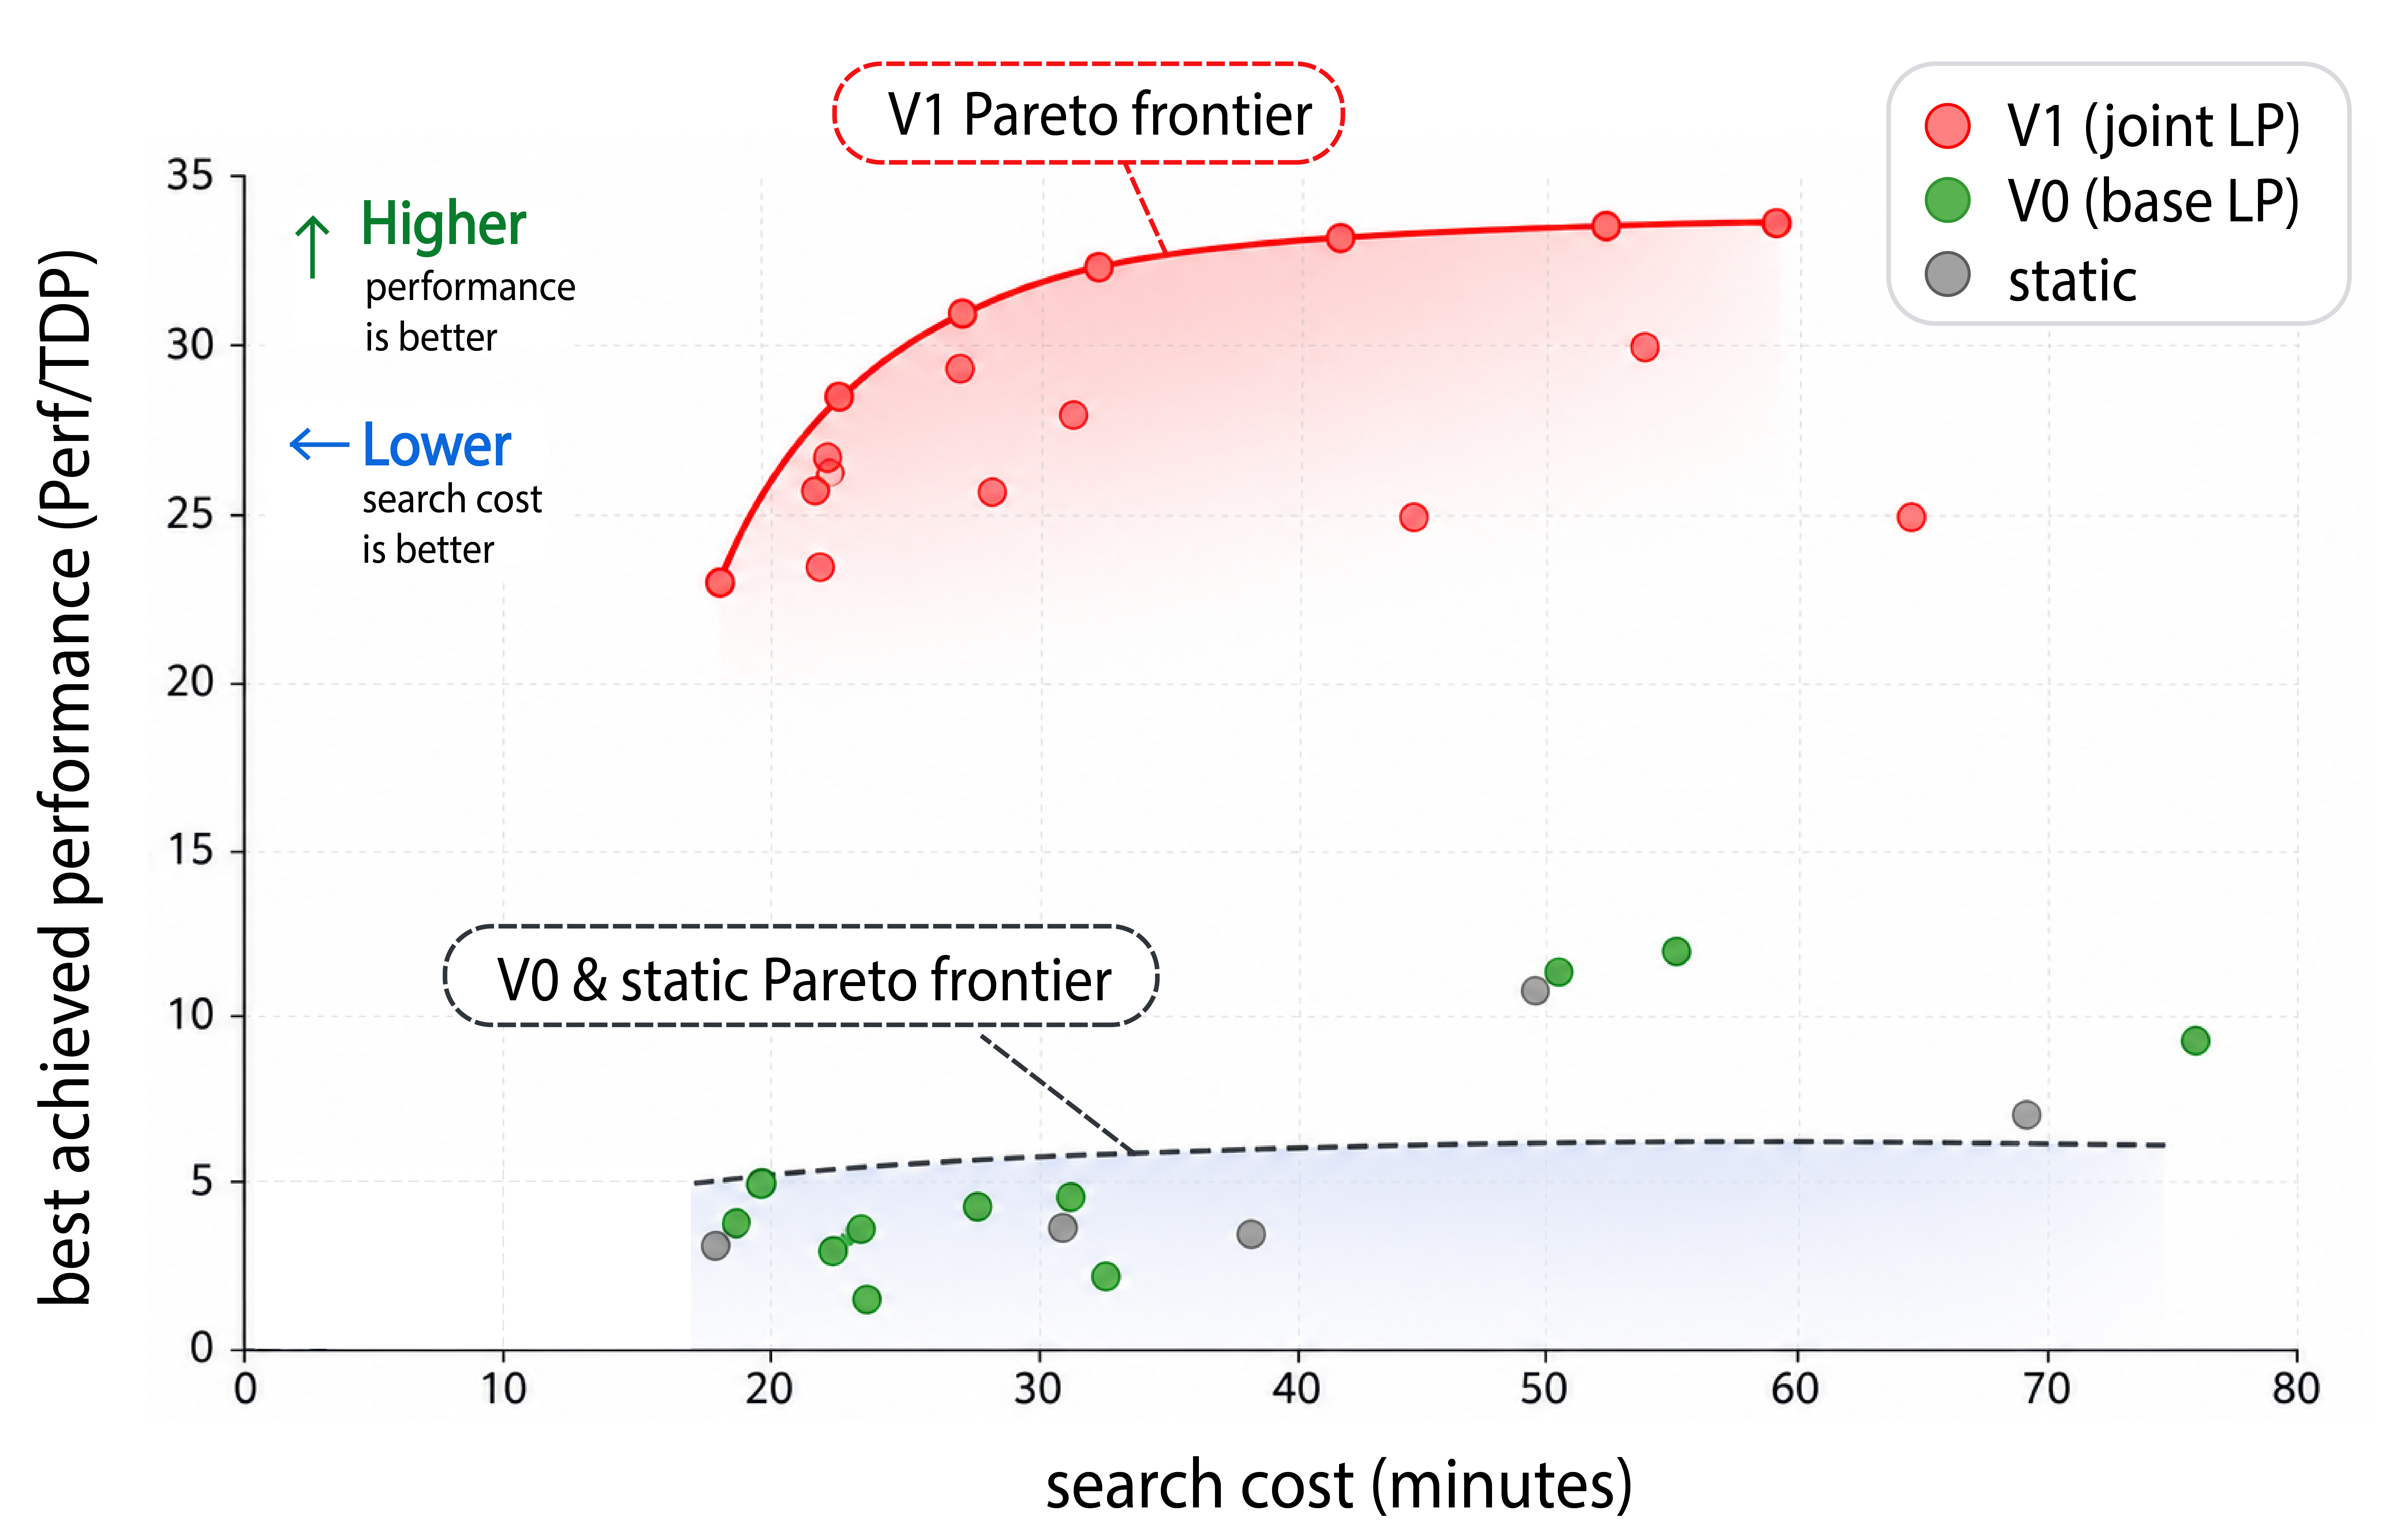
\includegraphics[width=0.7\linewidth]{figs/pareto_v2.png}
% % % %     \caption{pareto frontier plot}
% % % % \end{figure}
% % % \begin{figure}[ht!]
% % %     \centering
% % % 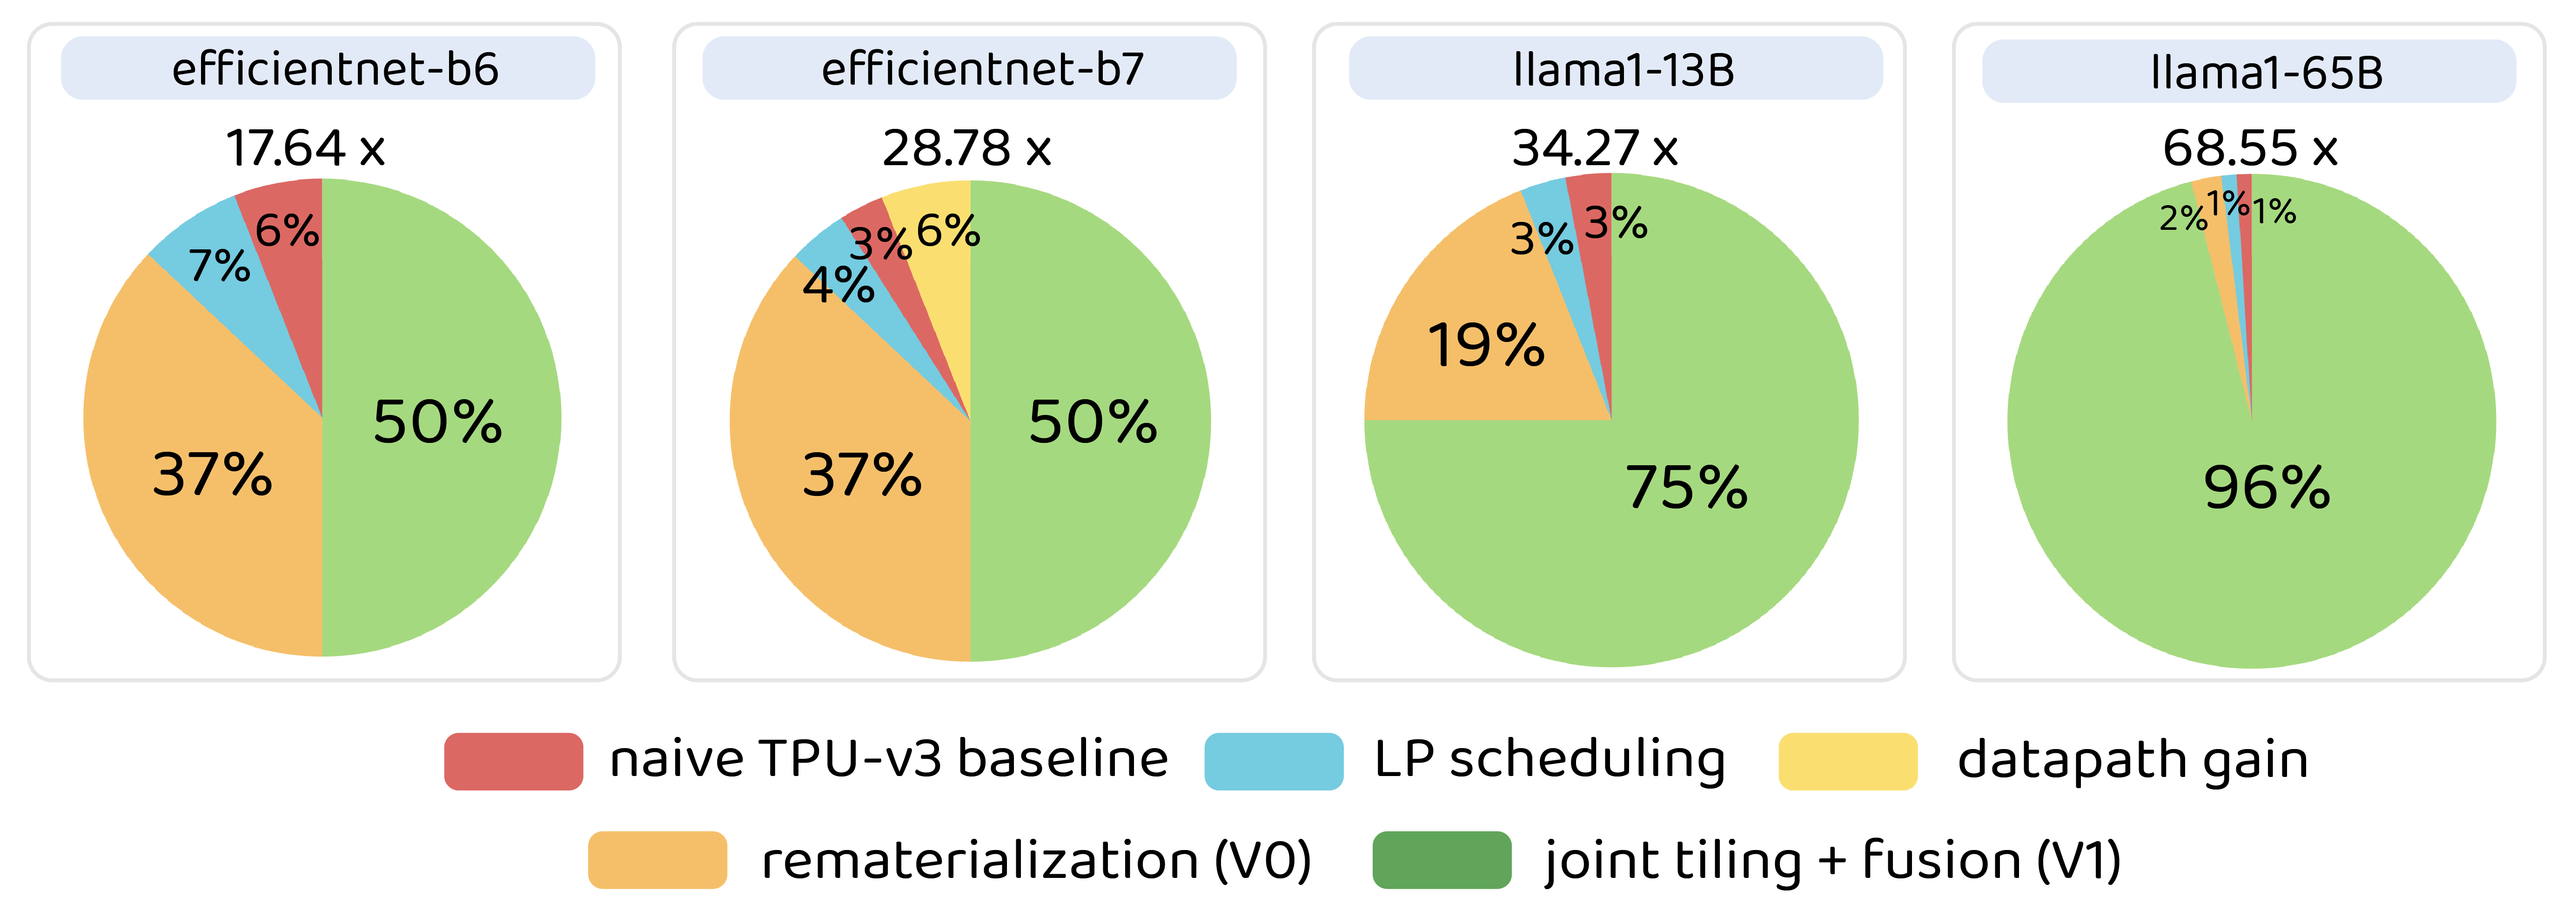
\includegraphics[width=0.85\linewidth]{fig3/speedup_decomposition_final_v2.png}
% % % \caption{Speedup decomposition over naive TPU-v3 baseline. Each pie shows the 
% % % relative contribution of four optimization sources to the total speedup. CHEETAH-V1 joint tiling + fusion dominates on all workloads, 
% % % especially on larger models where memory management is the primary bottleneck.}\label{fig:accel_decompose}
% % % \end{figure}
% % % \subsubsection{Static Baseline vs.\ CHEETAH-V0 vs.\ CHEETAH-V1 Unlock Progressive Gains}


% % % Figure~\ref{fig:accel_decompose} decomposes the total speedup over a naive TPU-v3 baseline into four sources: LP-based scheduling and fusion, datapath gain from hardware search, dynamic rematerialization (CHEETAH-V0), and joint tiling + fusion (CHEETAH-V1).

% % % The dominant contributor across all workloads is V1's joint tiling-fusion 
% % % optimization. On EfficientNet-B1, V1 accounts for 50\% of total speedup, 
% % % with LP scheduling (28\%) and datapath gain (22\%) splitting the remainder---and 
% % % no rematerialization benefit, consistent with B1's small activation footprint 
% % % fitting comfortably in Global Memory. B3--B4 show a similar 50\% V1 share, but 
% % % V0 rematerialization now contributes 25\%, reflecting the growing value of 
% % % recomputing large depthwise activations rather than reloading them from DRAM. 
% % % From B5 onward, V1's share rises sharply to 75--88\%, as the increasing 
% % % model size makes joint tiling-fusion the primary lever: memory management 
% % % dominates, and the remaining sources (LP scheduling, V0, datapath) each shrink 
% % % to single-digit percentages. The same pattern holds on Llama, where V1 accounts 
% % % for 83--87\% of the total speedup.

% % % % \begin{wrapfigure}{r}{0.48\textwidth}
% % % %     \centering
% % % %     \vspace{-12pt}
% % % %     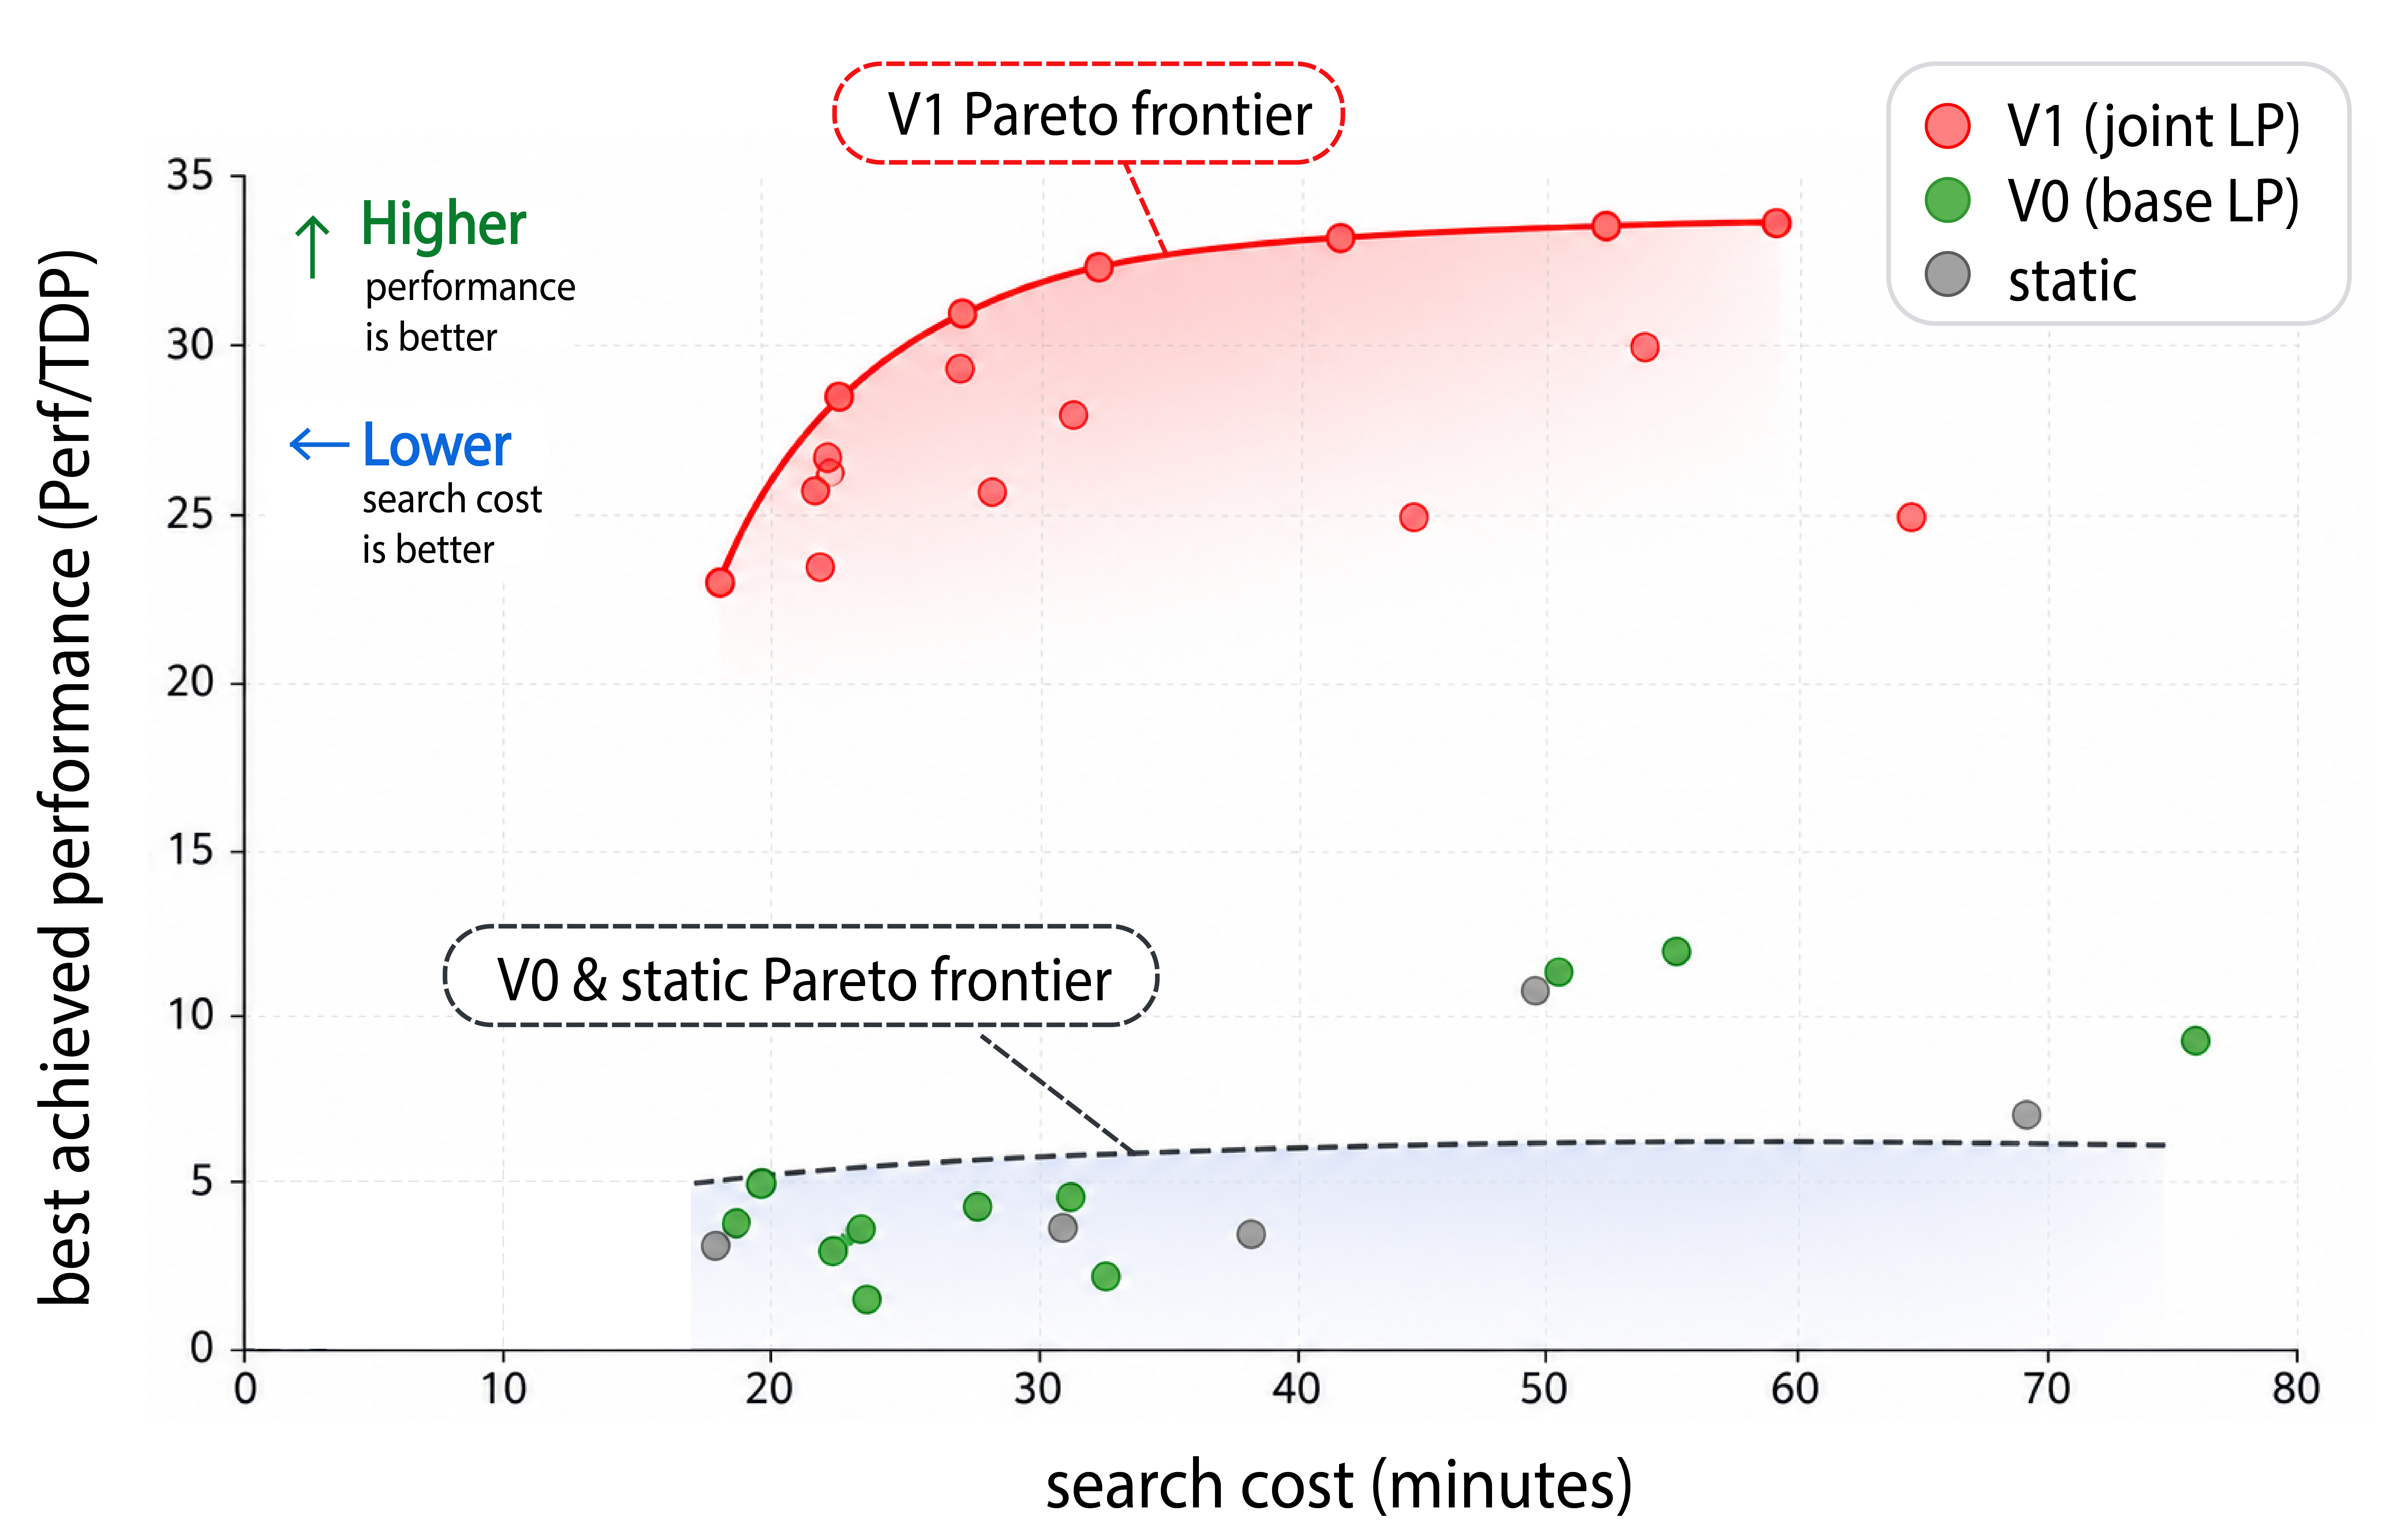
\includegraphics[width=0.48\textwidth]{figs/pareto_v2.png}
% % % %     \vspace{-18pt}
% % % %     \caption{Search cost vs.\ Perf/TDP Pareto frontier. V1 dominates V0 and static across all time budgets.}
% % % %     \label{fig:pareto}
% % % %     \vspace{-10pt}
% % % % \end{wrapfigure}

% % % Critically, Figure~\ref{fig:speedup} shows static fusion method is \emph{infeasible} on modern large models (Llama-70B, and DeepSeek-V3), because their large activation tensors cannot fit under a static pinning policy. The V0 formulation resolves feasibility for on large models via dynamic placement but remains time-intensive for a small number of 50 trials: measuring 58.42 hours on Llama-70B and 69.39 hours on DeepSeek-V3 (Figure~\ref{fig:wallclock}). In contrast Figures~\ref{fig:wallclock} and ~\ref{fig:speedup}, show the CHEETAH-V1 formulation out performs comparitive strategies in terms of speedup against the TPU-V3 baseline, and require only 1.17 hours on Llama-70B and 2.17 hours on DeepSeekv3 for 50 trails---a ${\sim}93\%$ average reduction. The powerful joint formulation is able to select memory-efficient tiling configurations alongside placement, achieving feasibility across the entire workload suite, demonstrating that joint optimization is not merely an incremental improvement but a qualitative capability unlock for large-scale models.

% % % % This demonstrates that by exploiting structural invariance and GPU-accelerated mathematical optimization, CHEETAH-V1 reduces the end-to-end co-design search time from days to under 2.2 hours—a ${\sim}93\%$ average reduction—while discovering architectural points that deliver up to $35\times$ speedup over the TPU-v3 baseline.

% % % % Figure~\ref{fig:pareto} shows the Pareto frontier of best-achieved Perf/TDP versus wall-clock search cost. V1 strictly dominates both V0 and static at every time budget: within 10 minutes of search, V1 already exceeds the best Perf/TDP that V0 or static achieve after 60+ minutes. The V1 Pareto frontier reaches ${\sim}35\times$ Perf/TDP, roughly $3\times$ higher than the V0/static frontier at ${\sim}10\text{--}12\times$. This gap reflects two compounding advantages: V1 explores a strictly larger feasible region (joint tiling-fusion), and it eliminates Timeloop from the per-trial critical path, allowing more trials within any fixed time budget.



% % % \paragraph{Practical insight.}
% % % Both LPs are extreme-aspect-ratio sparse: for \texttt{llama3\_70b},
% % % $m, n \sim 10^6$ and $\mathrm{nnz} \sim 5 \times 10^6$, giving roughly
% % % 1 nonzero per million matrix entries.
% % % The time-band structure means a coordinate-descent or stochastic PDHG
% % % solver would converge in $\mathcal{O}(T)$ sweeps if bands were the only
% % % structure.
% % % The capacity rows in both V0 and V1 LP formulations are the sole feature breaking strict banded structure, and they are precisely what couples the schedule globally. This is the desired behavior of a memory-aware placement formulation.

% % % % \todo{Report LP solve times for V0 and V1 across all benchmarks. Compare wall-clock time per trial against FAST's SCIP-based ILP solver (20 min timeout). Report LP relaxation gap: how often do fractional solutions need integer rounding, and what is the quality loss from rounding?}

% % % \paragraph{Structural invariance.}
% % % For a fixed workload and LP formulation, the LP constraint matrix
% % % has an invariant sparsity pattern across trials: the row/column
% % % dimensions and nonzero locations are determined only by the model graph structure — layer count $L$, timestep count $T$, edge set $E$, and Pareto count $C$ — not by the hardware candidate.
% % % Vizier changes only numerical values such as cycle coefficients,
% % % memory-capacity bounds, bandwidth-scaled access costs, objective weights, and TDP/area parameters. 
% % % This invariance allows us to reuse the same sparse matrix structure,
% % % variable ordering, block layout, and JIT-compiled sparse kernels in our adapted JAX PDLP solver across all hardware trials for a given workload.

% % % Numerically, we apply the same diagonal preconditioning pipeline
% % % on each trial: a structural presolve with 20 log-geomean Ruiz iterations, followed by the PDLP preprocessing stack with 10 infinity-norm Ruiz iterations and one Pock--Chambolle $\ell_1$-scaling pass. This two-stage diagonal scaling handles the mixed coefficient magnitudes present in V0/V1 matrices — large byte-valued capacity rows together with $\pm 1$ persistence rows — without requiring a fragile matrix factorization.

% % % In production, this preconditioning pipeline is reused structurally across trials, recomputes only cheap diagonal scalings, finishes in under one second for matrices with approximately $5 \times 10^6$ nonzeros, and avoids factorization failures entirely because it consists only of $D_1 A D_2$ arithmetic.

% % % \subsubsection{LLM Architect vs. Optimizer}
% % % The LLM Architect framework is modeled on SkyDiscover, and efficiently prunes the large outer hardware search loop by proposing campaign patches. Rather than predicting performance, the Architect reads a compact Causal Ledger containing invalid-rate history, MFU, roofline lower-bound checks, and LP diagnostics, then proposes a constrained hardware neighborhood for Vizier to search locally. The V1 LP remains the sole performance evaluator: for each candidate, it solves the joint tiling, fusion, placement, and rematerialization LP, while a deterministic Roofline Auditor rejects physically impossible results. In the widened V1 search space, all methods reach the same capped V1 Perf/TDP ceiling, so the key differentiator is search efficiency. The LLM loop reduces invalid hardware evaluations from 24.5\% under full-space Vizier to 5.9\% on average across five workloads, a 4.1× reduction in wasted trials, while preserving the same best V1 score. This shows that the LLM’s contribution is not replacing Vizier or the solver, but steering Bayesian optimization toward feasible, workload-appropriate architectural neighborhoods with far less wasted trials. This also sets the foundation for future work, where the LLM in the loop can adhere to follow more complex human reasoning signals.
% % % \begin{figure}[ht!]
% % %     \centering
% % % 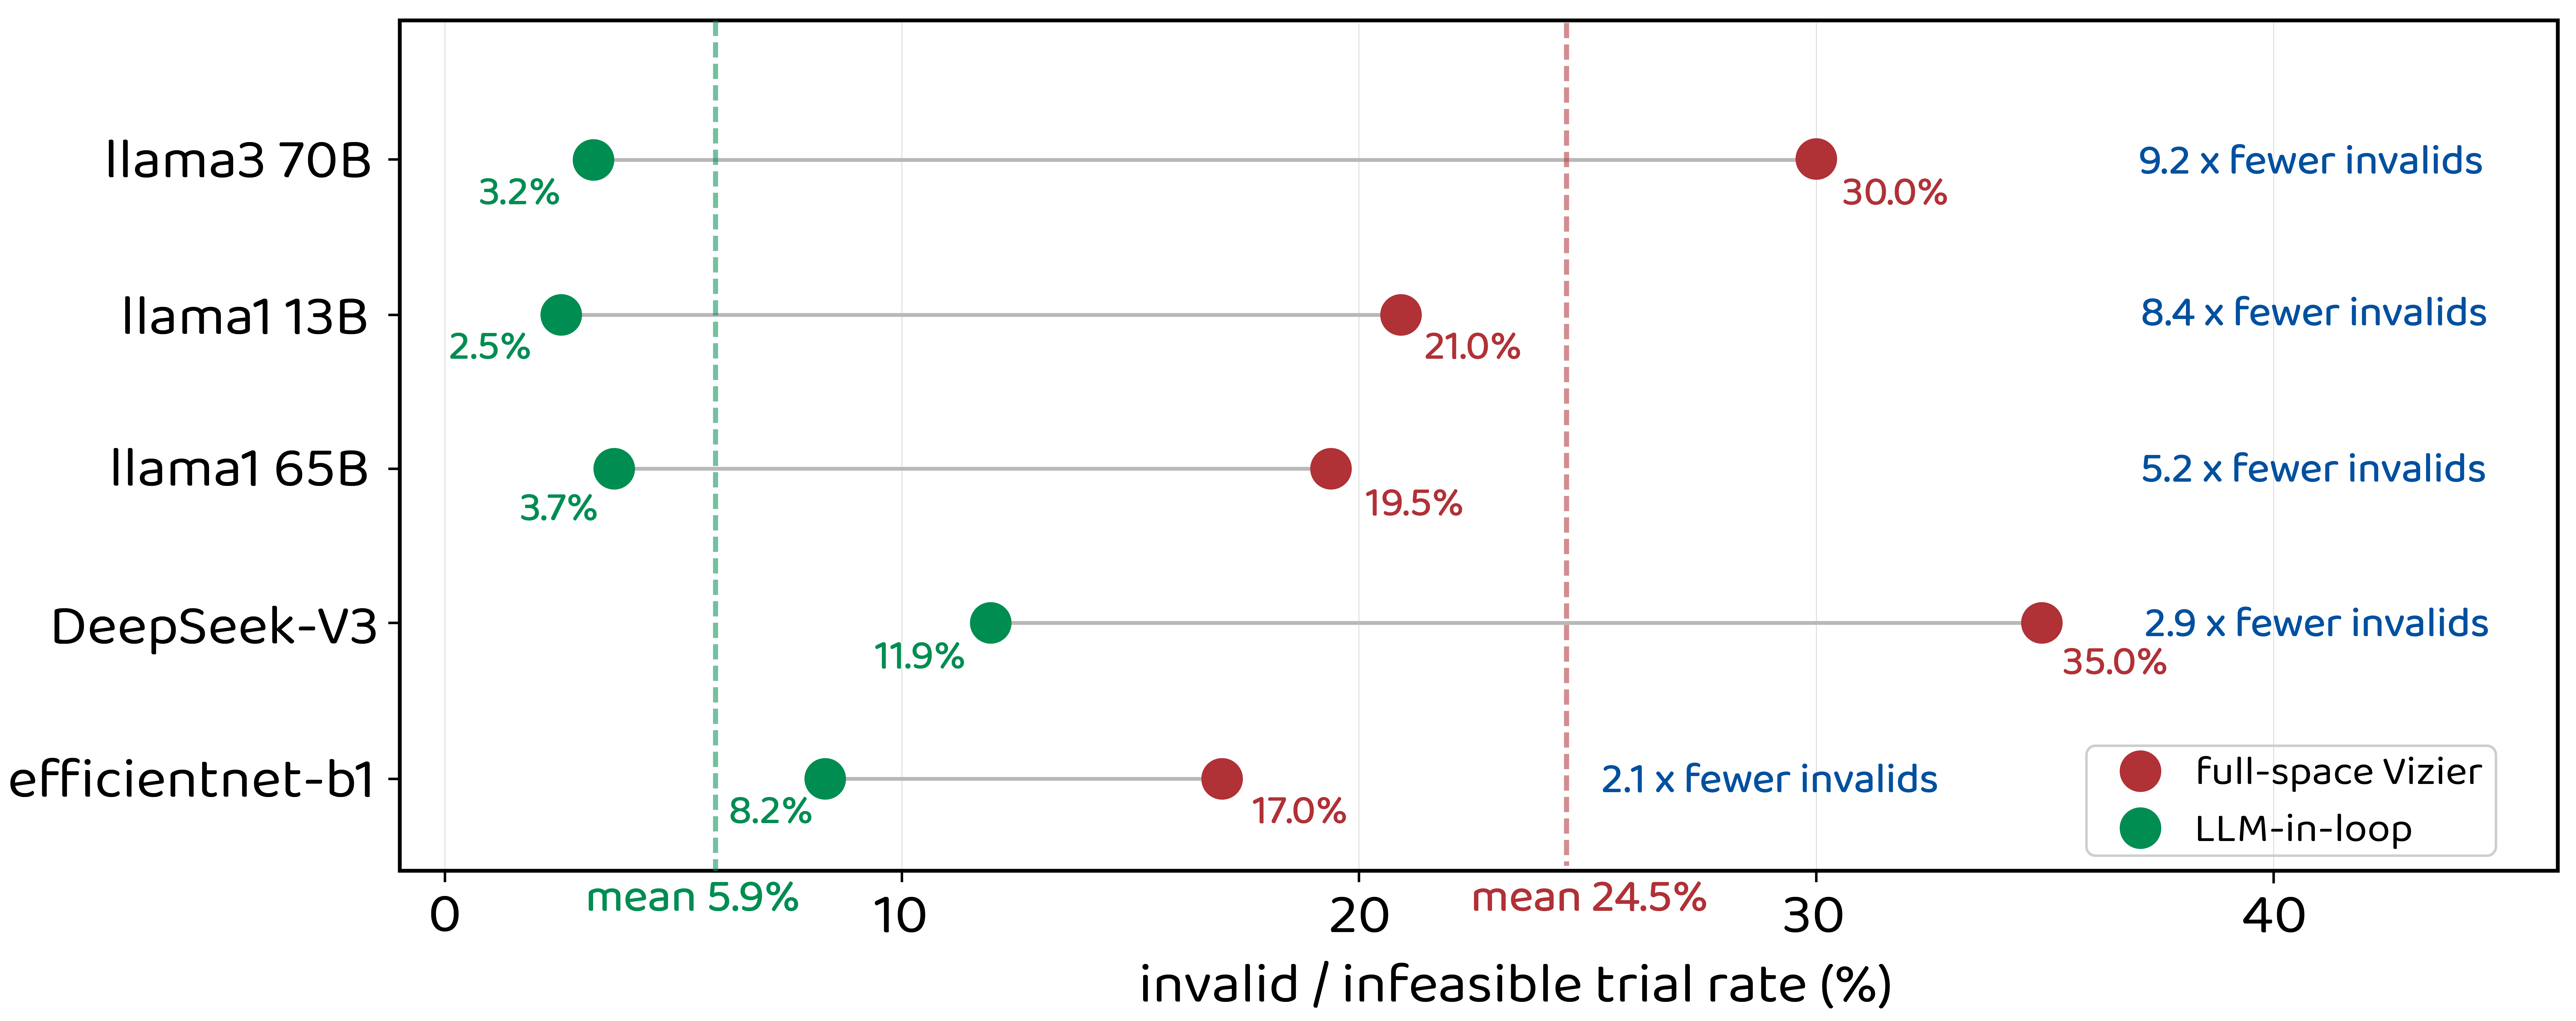
\includegraphics[width=0.85\linewidth]{fig3/llm_guide_v1.png}
% % % \caption{Strategic Intelligence vs. Stochastic Brute Force}\label{fig:llm}
% % % \end{figure}



% % % % The LLM should not just ask, “What chip has the best Perf/TDP?” We aim to answer the question “Given this user’s workload and deployment goal, what is the architectural region to search for this deployment task?”. Therefore we have the LLM emit profile-conditioned campaigns that take specific user inference tasks into consideration. For each $(\text{deployment profile},\ \text{workload})$ cell, we ran a
% % % % 200-trial LLM-Architect experiment using the same Qwen2.5-7B-Instruct + LoRA with differing user input profiles. At the start of each round, the prompt was assembled from a fixed system
% % % % prompt, the active deployment profile, three few-shot examples, and a per-round user message containing the workload, recent feedback signals, current search bounds, and the causal ledger.
% % % % The Strategist returned a one-line JSON campaign patch, which the
% % % % validator accepted only if it was a strict legal subset of the parent space, satisfied hard rules such as patch-volume $\leq 10\%$, ridgepoint and MAC/BW constraints, and avoided forbidden regions.

% % % % Thus, the experiment isolates whether the profile-conditioned LLM prompt alone can steer the same V1 evaluator toward different hardware families under different deployment intents.



% % % % \todo{Compare convergence rate of LLM-guided hardware search vs.\ Vizier-only (Bayesian, LCS, random baselines) in the style of FAST Figure~11. Report:
% % % % \begin{itemize}
% % % %     \item Number of trials to reach $X\%$ of best Perf/TDP found by 5,000-trial Vizier
% % % %     \item Quality of LLM-proposed configurations vs.\ Vizier-proposed configurations
% % % %     \item Qualitative analysis of LLM reasoning about hardware bottlenecks
% % % % \end{itemize}
% % % % }

% % % % \subsubsection{ROI Analysis}

% % % % \todo{Update FAST's ROI analysis (Table~4) with the improved Perf/TDP numbers from FAST-CORGI. Report deployment volumes required to reach 1$\times$, 2$\times$, 4$\times$ ROI targets. If Perf/TDP improvements are larger than FAST's, the break-even deployment volume should decrease correspondingly.}

% % % % \subsubsection{Pareto Frontier}

% % % % \todo{Plot the Perf/TDP vs.\ area Pareto frontier for V1-optimized designs compared to FAST and TPU-v3 baseline, analogous to FAST Figure~12.}


% % % edit for page limit

% % \section{Experiments}
% % \label{sec:experiments}
% % We implement an adapted JAX PDLP solver for large-scale models (Llama-70B and DeepSeek-V3) across all formulations (Static, V0, V1), while employing HiGHS for smaller networks. To maintain consistency with prior research, results are reported as speedup relative to a simulated TPU-v3 baseline. The TPU-v3 is selected as a benchmark because its architecture is purpose-built for neural network acceleration and its publicly available specifications permit high-fidelity simulation.

% % \subsection{Experimental Setup}

% % \paragraph{Static Sequential Baseline.}
% % We compare against the static optimization FAST framework using a simulated TPU-v3 baseline normalized to a sub-10nm process technology, following the same methodology as Zhang \etal. The baseline simulator is well-correlated with production hardware: on average within 8.2\,$\pm$\,2.7\% of profiled TPU-v3 performance. We evaluate against a \emph{simulated} TPU-v3 baseline to account for optimistic simulator assumptions. We evaluate across 11 representative workloads: EfficientNet-B1 through EfficientNet-B7, Llama13, 65, 70 models, and DeepSeek-V3-MoE. These workloads stress different parts of the hardware design space: EfficientNet stresses low-operational-intensity depthwise convolutions, while Llama and DeepSeek stress memory capacity, bandwidth, and large matrix operations. 

% % \textbf{Single-workload specialization.} Each neural network workload is optimized independently. This experiment measures the best workload-specific hardware found under a fixed trial budget and identifies architectural preferences such as Global Memory size, bandwidth, MAC count, and systolic shape. In the case of Staitic and V0 methods, the pipeline involves: Vizier - Timeloop - LP solver. In the case of the V1 method, the pipeline is simplified to Vizier - LP solver. In each case we iterate for 100 trials per method x NN. 

% % % \textbf{Fixed-hardware-workload generalization.} We search for general-purpose datapaths that perform well across the workload suite. The objective is a harmonic or geometric aggregation of per-workload Perf/TDP, forcing the search to balance CNN-style memory pressure and LLM-style compute/memory trade-offs.

% % \textbf{LLM-Architect guides outer search.} We the LLM-guided outer-loop controller which proposes search-space interventions for Vizier. The advantage of the CHEETAH-V1 formulation is it removes dependence of Timeloop in the loop. Therefore the loop is reduced to just Vizier-LP solve, which dramatically speeds up the iterative process, thus permitting the LLM-Architect outer loop. The LLM is only permitted to change the search neighborhood of Vizier's input, the strict LP formulation on the inner loop does not change. This ensures mathematical and physical constraints are upheld in the space of co-design. We validate all results through a multi-level audit process---Roofline Auditor, Campaign Validator, Causal Ledger, and solver diagnostics (primal/dual residuals, duality gap)---as described in Section~\ref{sec:llm_outer} and detailed in Appendix~\ref{app:validation}. All reported V0/V1 results are roofline-feasible with zero lower-bound violations.

% % % \paragraph{Optimization framework.}
% % % For the outer hardware search loop, we use Google Vizier with LCS optimization and safe search, running 100 trials per experiment (method X NN x Exp). Each trial invokes the LP solver for the inner optimization. The Static and V0 methods additionally have Timeloop in the loop (Vizier-Timeloop-LP solve). The advantage of the v1 formulation is it removes dependance of Timeloop in the loop. Therefore the loop is reduced to just Vizier-Lp solve, which dramatically speeds up the iterative process, thus permitted the Strategic LLM outer loop.




% % \subsection{Main Results}

% % % \subsubsection{V0 vs.\ FAST Static Fusion}

% % % \todo{Insert results table and figure comparing V0 (time-indexed placement + rematerialization) against FAST's static fusion ILP on all benchmarks. Key metrics: Perf/TDP improvement, fusion efficiency (\% of DRAM stall time eliminated), rematerialization frequency (how often does the solver choose to recompute rather than reload?).}

% % % \paragraph{Expected findings.}
% % % V0's dynamic placement should show the largest gains on workloads with: (1)~tight Global Memory budgets where static pinning wastes capacity on tensors that are only needed briefly, (2)~long dependency chains where tensor lifetimes vary substantially, and (3)~cheap-to-recompute operations with large activations (\eg, depthwise convolutions in EfficientNet).

% % % \subsubsection{V1 vs.\ V0: Joint Tiling and Fusion}

% % % \todo{Insert results table and figure comparing V1 against V0 on all benchmarks. Key metrics: Perf/TDP improvement, number of operations where V1 selects a different tiling configuration than Timeloop's greedy choice, and the resulting compute efficiency vs.\ fusion trade-off.}

% % % \paragraph{Expected findings.}
% % % V1 should show the largest gains on architectures with highly diverse layer types where a single tiling configuration cannot serve all operations well. EfficientNet (depthwise + pointwise convolutions with 100$\times$ variation in working-set sizes) and hybrid CNN-transformer models (convolutions + attention + MLP with fundamentally different compute-memory profiles) are expected to benefit most.


% % % \subsubsection{stiatic vs v0 vs v1}
% % % \begin{figure}[ht!]
% % %     \centering
% % %     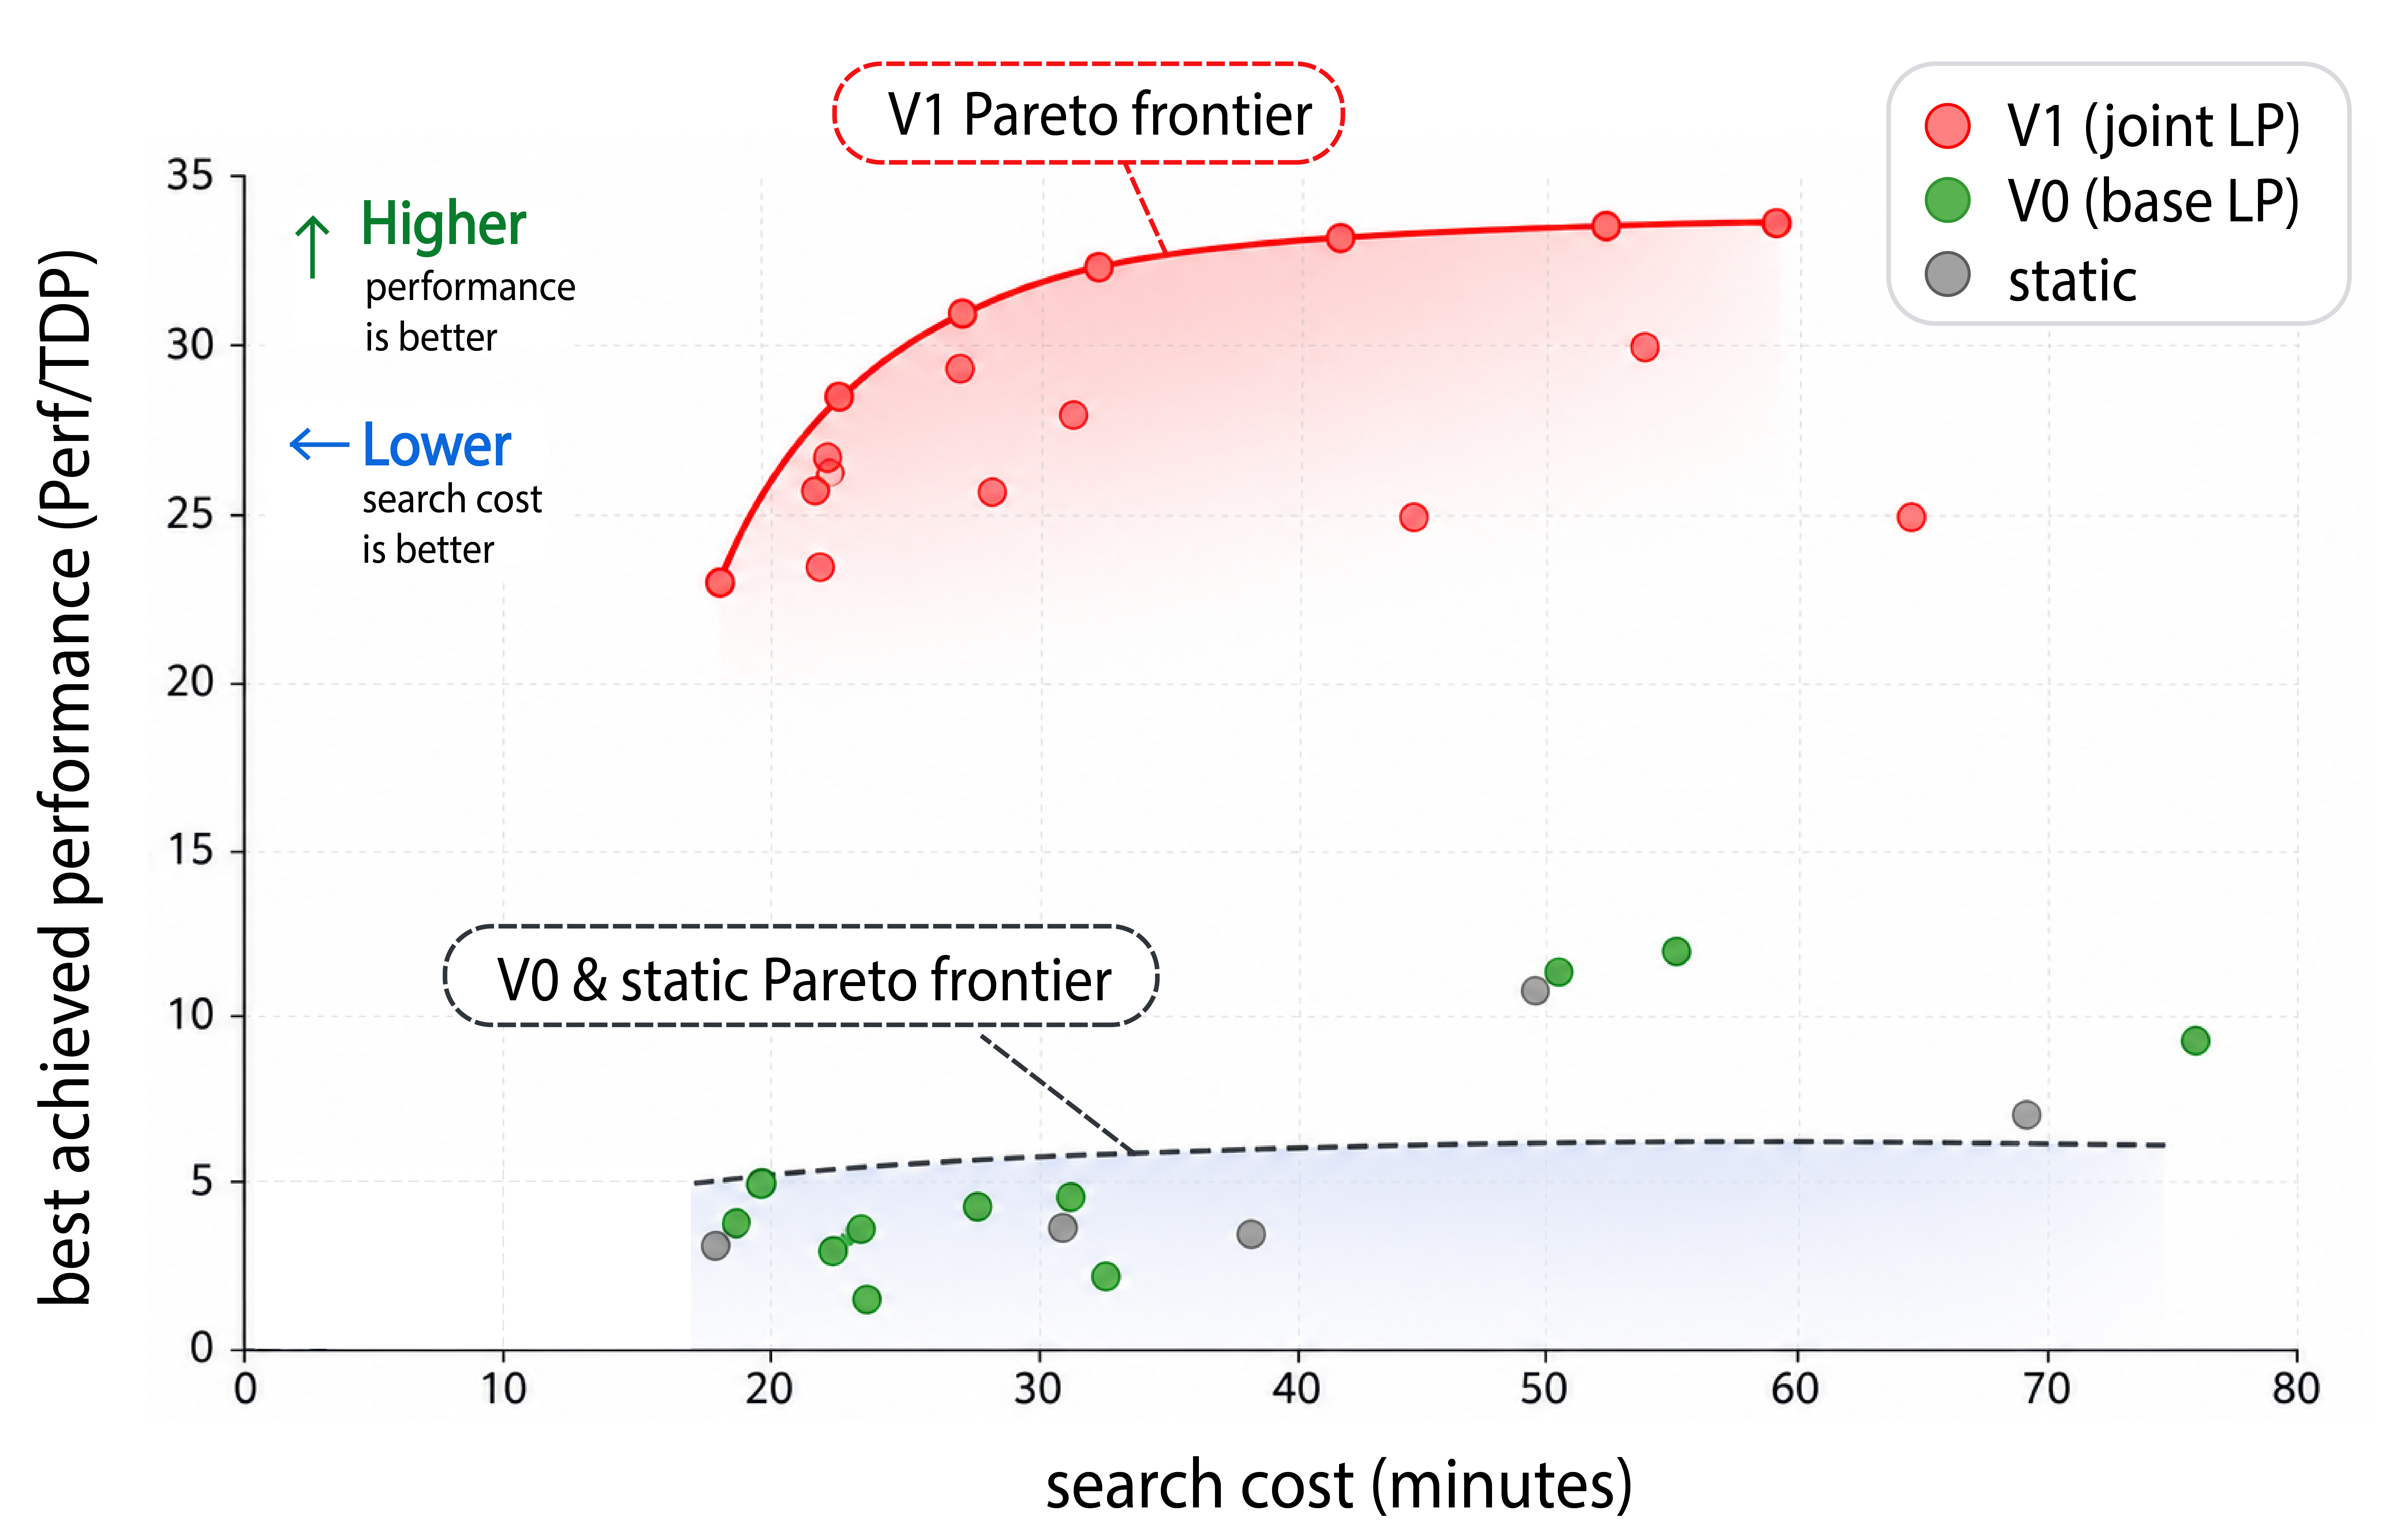
\includegraphics[width=0.7\linewidth]{figs/pareto_v2.png}
% % %     \caption{pareto frontier plot}
% % % \end{figure}
% % \begin{figure}[ht!]
% %     \centering
% % 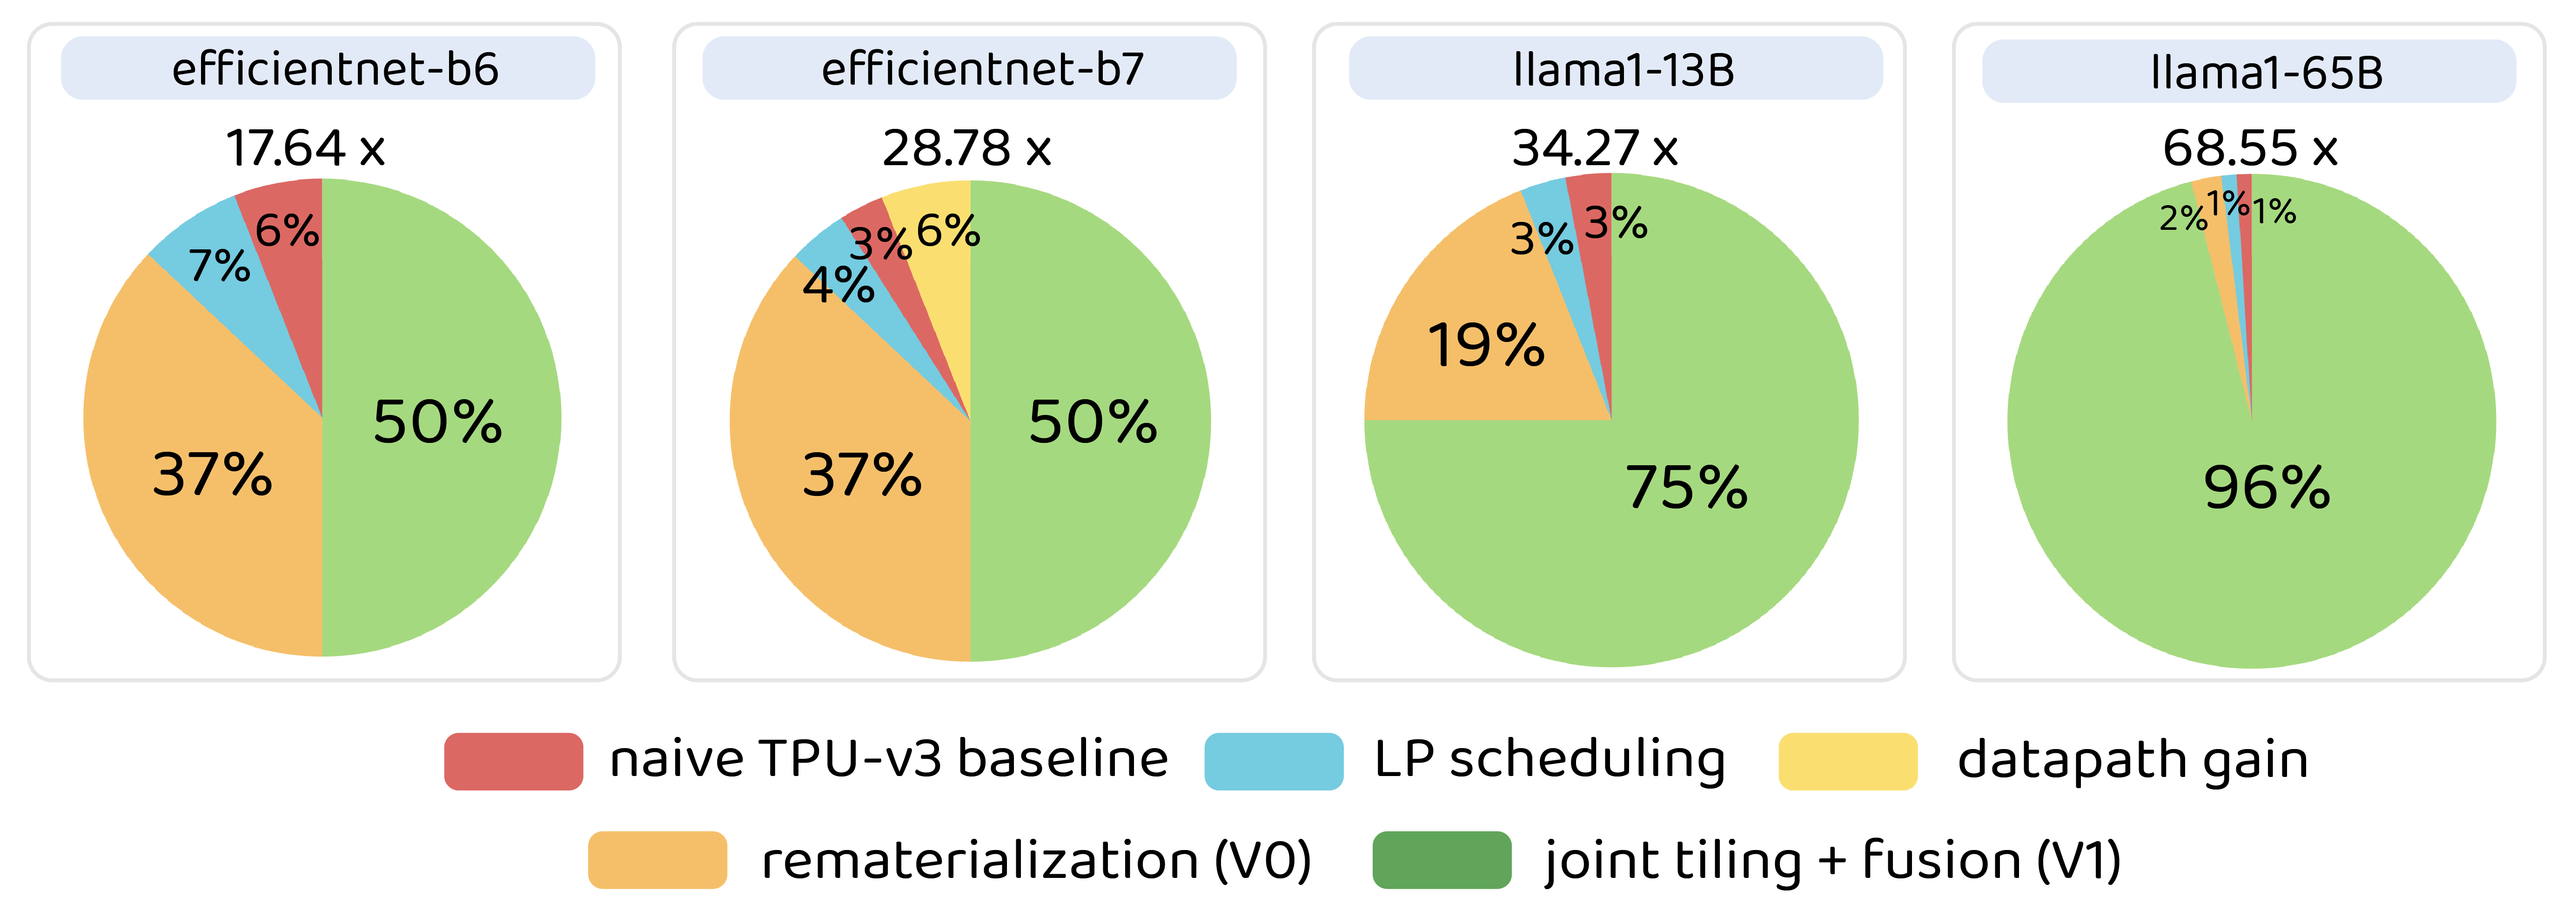
\includegraphics[width=0.85\linewidth]{fig3/speedup_decomposition_final_v2.png}
% % \caption{Speedup decomposition over naive TPU-v3 baseline. Each pie shows the 
% % relative contribution of four optimization sources to the total speedup. CHEETAH-V1 joint tiling + fusion dominates on all workloads, 
% % especially on larger models where memory management is the primary bottleneck.}\label{fig:accel_decompose}
% % \end{figure}
% % \paragraph{CHEETAH-V0 vs.\ CHEETAH-V1 Unlock Progressive Gains.} Figure~\ref{fig:accel_decompose} decomposes the total speedup over a naive TPU-v3 baseline into four sources: LP-based scheduling and fusion, datapath gain from hardware search, dynamic rematerialization (CHEETAH-V0), and joint tiling + fusion (CHEETAH-V1).

% % The dominant contributor across all workloads is V1's joint tiling-fusion 
% % optimization. On EfficientNet-B1, V1 accounts for 50\% of total speedup, 
% % with LP scheduling (28\%) and datapath gain (22\%) splitting the remainder---and 
% % no rematerialization benefit, consistent with B1's small activation footprint 
% % fitting comfortably in Global Memory. B3--B4 show a similar 50\% V1 share, but 
% % V0 rematerialization now contributes 25\%, reflecting the growing value of 
% % recomputing large depthwise activations rather than reloading them from DRAM. 
% % From B5 onward, V1's share rises sharply to 75--88\%, as the increasing 
% % model size makes joint tiling-fusion the primary lever: memory management 
% % dominates, and the remaining sources (LP scheduling, V0, datapath) each shrink 
% % to single-digit percentages. The same pattern holds on Llama, where V1 accounts 
% % for 83--87\% of the total speedup.

% % % \begin{wrapfigure}{r}{0.48\textwidth}
% % %     \centering
% % %     \vspace{-12pt}
% % %     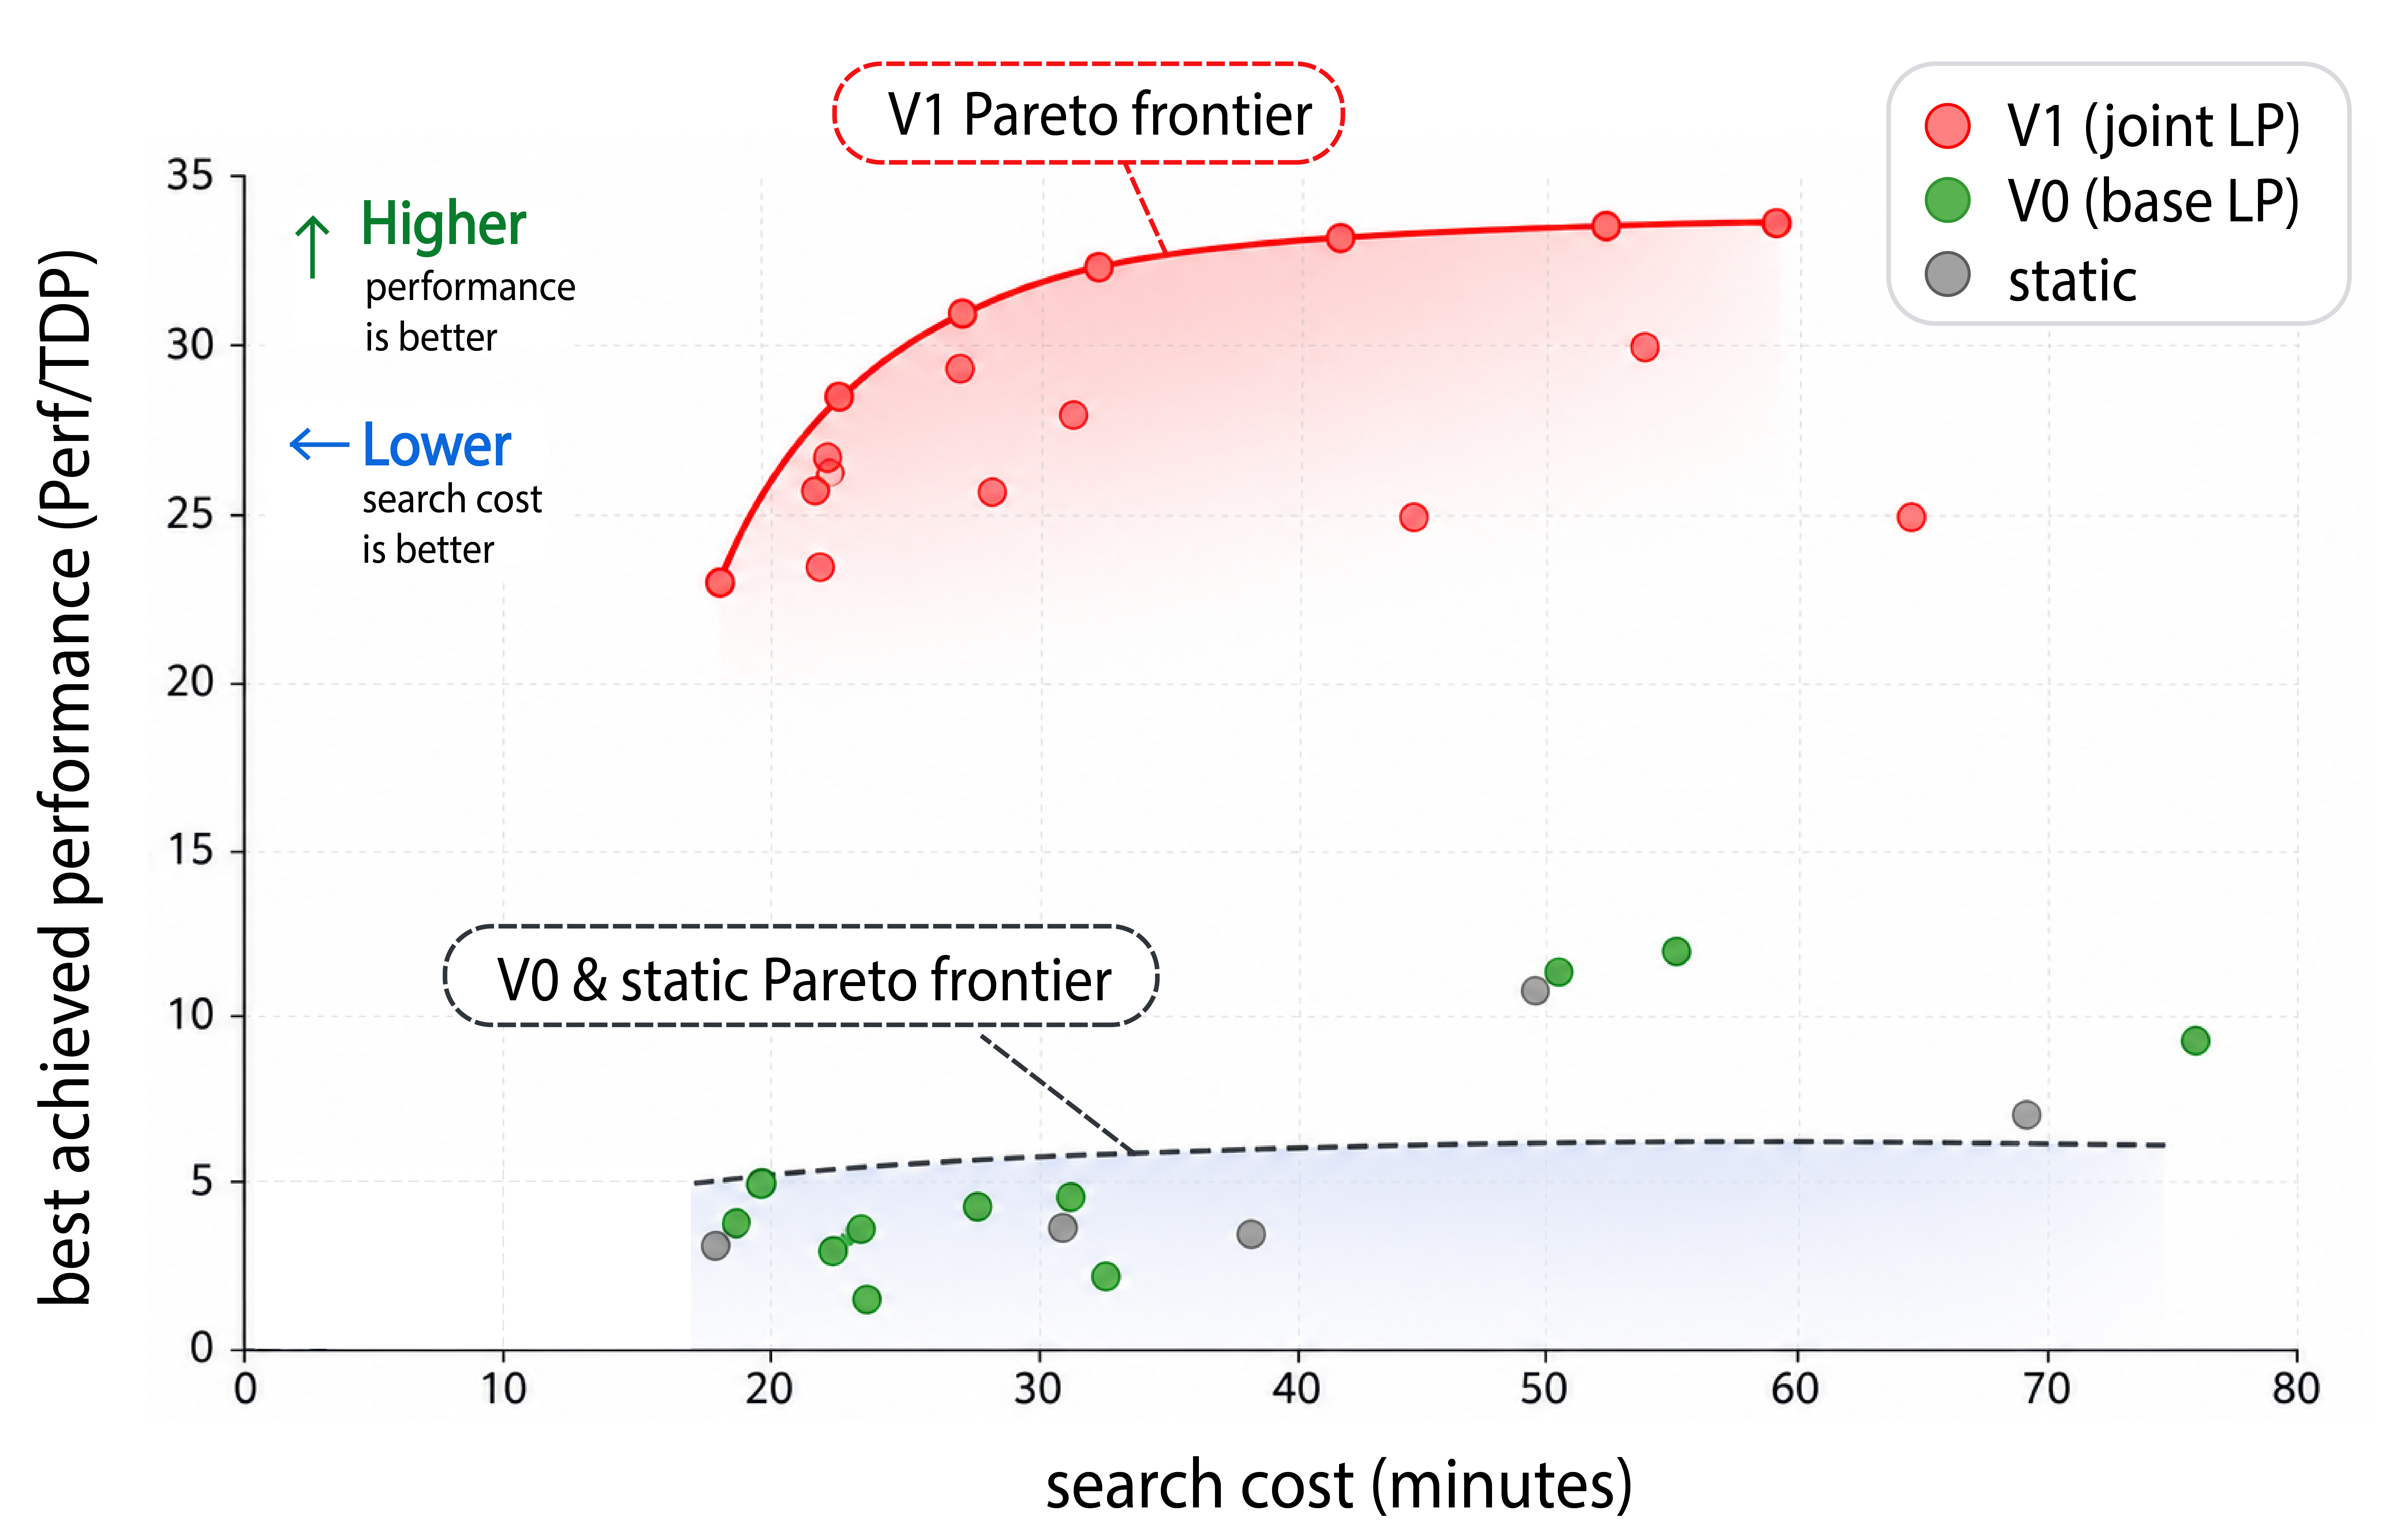
\includegraphics[width=0.48\textwidth]{figs/pareto_v2.png}
% % %     \vspace{-18pt}
% % %     \caption{Search cost vs.\ Perf/TDP Pareto frontier. V1 dominates V0 and static across all time budgets.}
% % %     \label{fig:pareto}
% % %     \vspace{-10pt}
% % % \end{wrapfigure}

% % Critically, Figure~\ref{fig:speedup} shows static fusion method is \emph{infeasible} on modern large models (Llama-70B, and DeepSeek-V3), because their large activation tensors cannot fit under a static pinning policy. The V0 formulation resolves feasibility for on large models via dynamic placement but remains time-intensive for a small number of 50 trials: measuring 58.42 hours on Llama-70B and 69.39 hours on DeepSeek-V3 (Figure~\ref{fig:wallclock}). In contrast Figures~\ref{fig:wallclock} and ~\ref{fig:speedup}, show the CHEETAH-V1 formulation out performs comparitive strategies in terms of speedup against the TPU-V3 baseline, and require only 1.17 hours on Llama-70B and 2.17 hours on DeepSeekv3 for 50 trails---a ${\sim}93\%$ average reduction. The powerful joint formulation is able to select memory-efficient tiling configurations alongside placement, achieving feasibility across the entire workload suite, demonstrating that joint optimization is not merely an incremental improvement but a qualitative capability unlock for large-scale models.

% % % This demonstrates that by exploiting structural invariance and GPU-accelerated mathematical optimization, CHEETAH-V1 reduces the end-to-end co-design search time from days to under 2.2 hours—a ${\sim}93\%$ average reduction—while discovering architectural points that deliver up to $35\times$ speedup over the TPU-v3 baseline.

% % % Figure~\ref{fig:pareto} shows the Pareto frontier of best-achieved Perf/TDP versus wall-clock search cost. V1 strictly dominates both V0 and static at every time budget: within 10 minutes of search, V1 already exceeds the best Perf/TDP that V0 or static achieve after 60+ minutes. The V1 Pareto frontier reaches ${\sim}35\times$ Perf/TDP, roughly $3\times$ higher than the V0/static frontier at ${\sim}10\text{--}12\times$. This gap reflects two compounding advantages: V1 explores a strictly larger feasible region (joint tiling-fusion), and it eliminates Timeloop from the per-trial critical path, allowing more trials within any fixed time budget.



% % \paragraph{Practical insight.}
% % Both LPs are extreme-aspect-ratio sparse: for \texttt{llama3\_70b},
% % $m, n \sim 10^6$ and $\mathrm{nnz} \sim 5 \times 10^6$, giving roughly
% % 1 nonzero per million matrix entries.
% % The time-band structure means a coordinate-descent or stochastic PDHG
% % solver would converge in $\mathcal{O}(T)$ sweeps if bands were the only
% % structure.
% % The capacity rows in both V0 and V1 LP formulations are the sole feature breaking strict banded structure, and they are precisely what couples the schedule globally. This is the desired behavior of a memory-aware placement formulation.

% % % \todo{Report LP solve times for V0 and V1 across all benchmarks. Compare wall-clock time per trial against FAST's SCIP-based ILP solver (20 min timeout). Report LP relaxation gap: how often do fractional solutions need integer rounding, and what is the quality loss from rounding?}

% % \paragraph{Structural invariance.}
% % For a fixed workload and LP formulation, the LP constraint matrix
% % has an invariant sparsity pattern across trials: the row/column
% % dimensions and nonzero locations are determined only by the model graph structure — layer count $L$, timestep count $T$, edge set $E$, and Pareto count $C$ — not by the hardware candidate.
% % Vizier changes only numerical values such as cycle coefficients,
% % memory-capacity bounds, bandwidth-scaled access costs, objective weights, and TDP/area parameters. 
% % This invariance allows us to reuse the same sparse matrix structure,
% % variable ordering, block layout, and JIT-compiled sparse kernels in our adapted JAX PDLP solver across all hardware trials for a given workload. We apply the same diagonal preconditioning pipeline
% % on each trial: a structural presolve with 20 log-geomean Ruiz iterations, followed by the PDLP preprocessing stack with 10 infinity-norm Ruiz iterations and one Pock--Chambolle $\ell_1$-scaling pass. This two-stage diagonal scaling handles the mixed coefficient magnitudes present in V0/V1 matrices — large byte-valued capacity rows together with $\pm 1$ persistence rows — without requiring a fragile matrix factorization. In production, this preconditioning pipeline is reused structurally across trials, recomputes only cheap diagonal scalings, finishes in under one second for matrices with approximately $5 \times 10^6$ nonzeros, and avoids factorization failures entirely because it consists only of $D_1 A D_2$ arithmetic.

% % \paragraph{LLM Architect vs.\ Optimizer.} 
% % \begin{wrapfigure}{r}{0.50\textwidth}
% %     \centering
% %     \vspace{-6pt}
% %     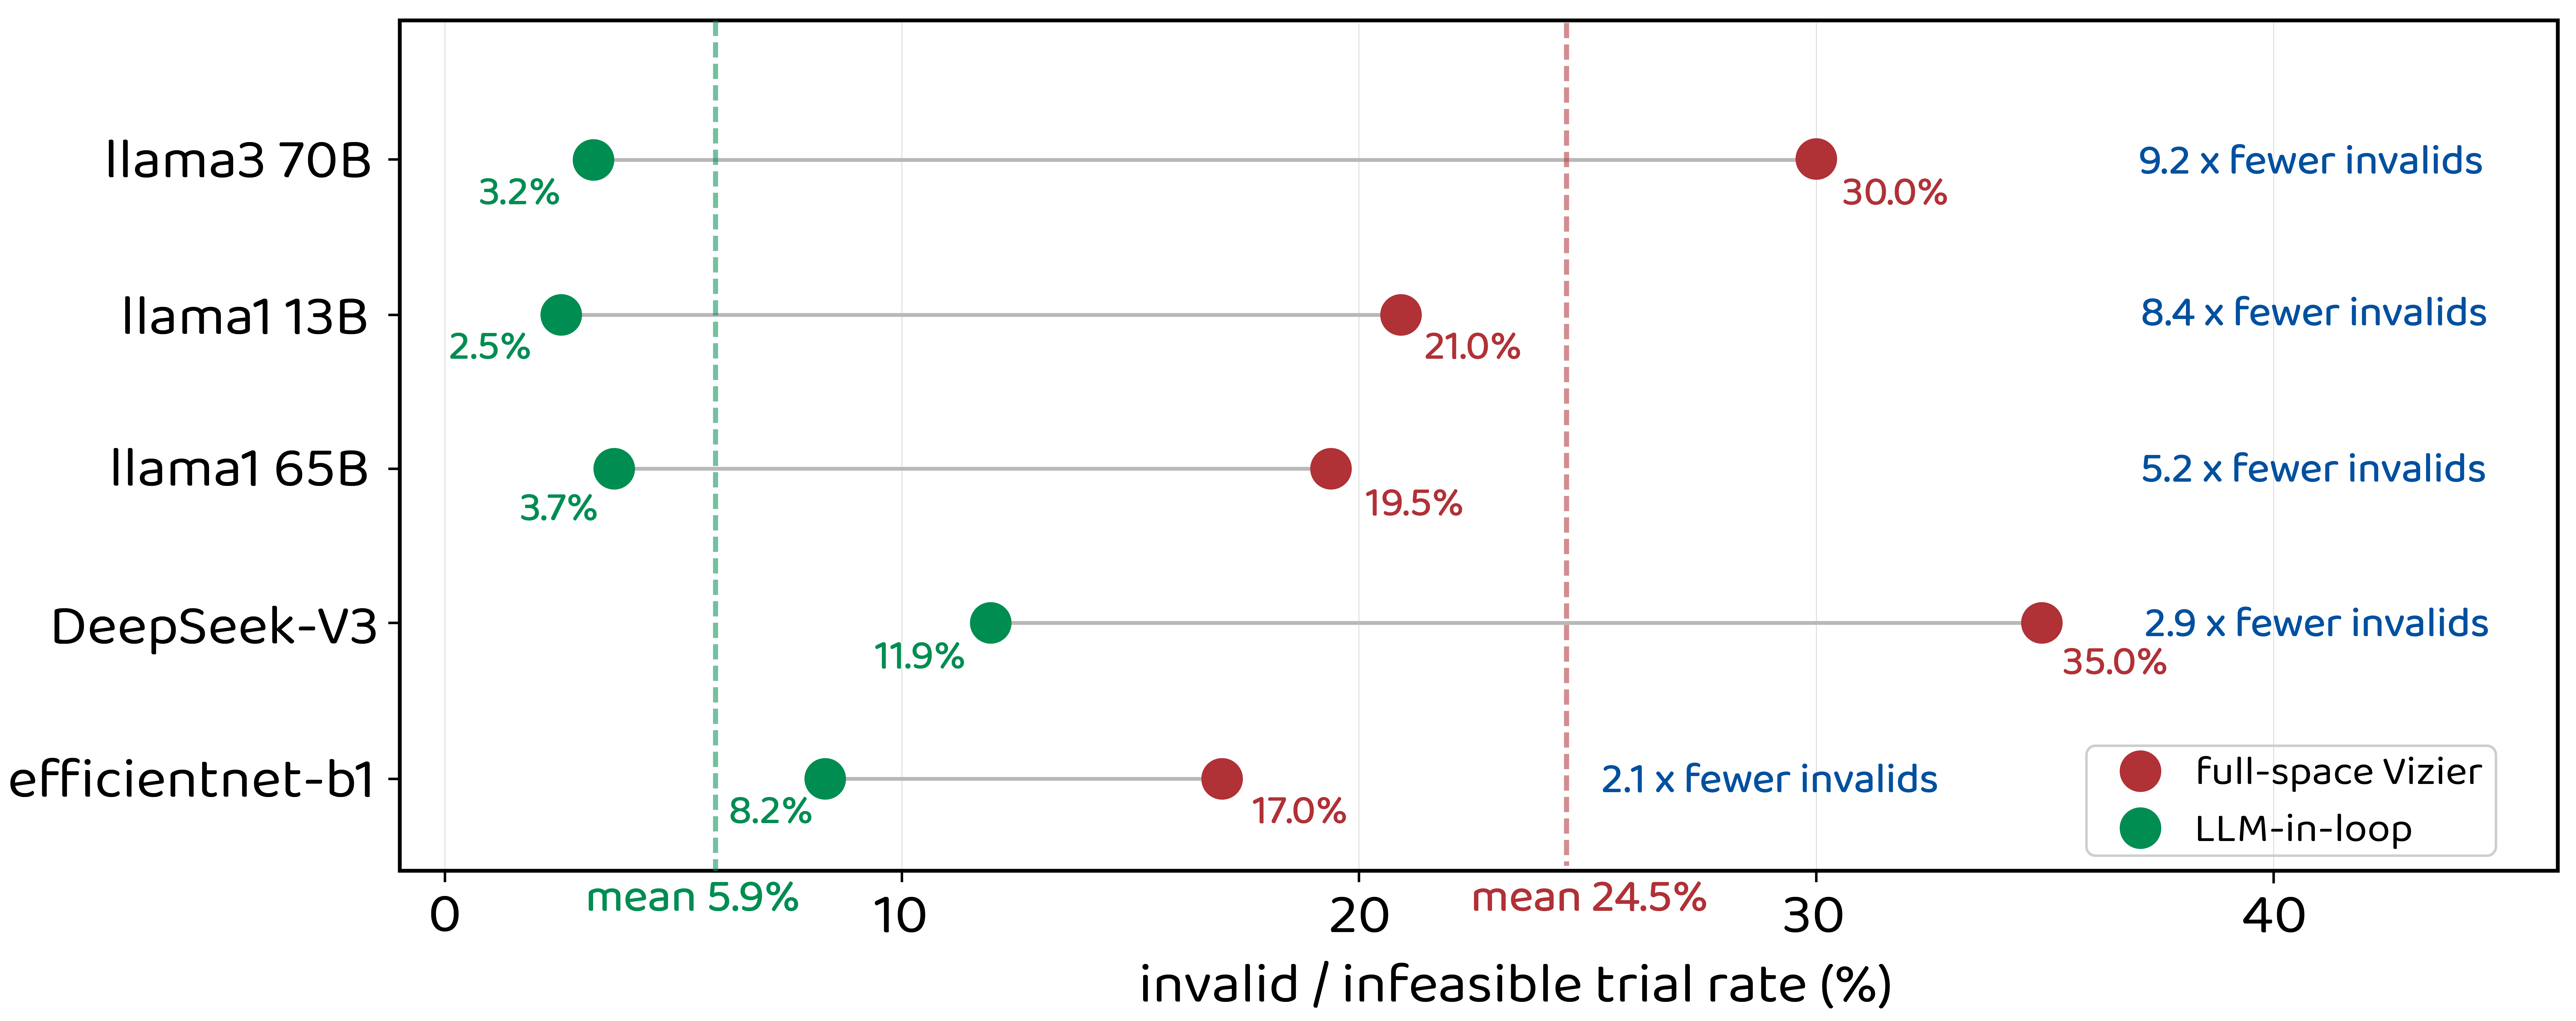
\includegraphics[width=0.48\textwidth]{fig3/llm_guide_v1.png}
% %     \caption{Strategic Intelligence vs.\ Stochastic Brute Force. Green indicates the LLM-Architect has less wasted trials.}
% %     \label{fig:llm}
% %     \vspace{-10pt}
% % \end{wrapfigure}

% % Modelled on SkyDiscovery~\citep{skydiscover2026}, the LLM Architect prunes
% % the outer search loop by proposing campaign patches rather than
% % predicting raw performance. It analyses a Causal Ledger containing
% % invalid rates, MFU, and solver diagnostics to suggest constrained
% % hardware neighbourhoods for Vizier to explore locally. The V1 LP
% % remains the ground-truth evaluator, supported by a Roofline Auditor
% % that rejects physically impossible results.
% % In a widened search space, the LLM loop reduces invalid evaluations
% % from $24.5\%$ to $5.9\%$ on average — a $4.1\times$ reduction in wasted
% % trials — while reaching the same optimal Perf/TDP scores as full-space
% % Vizier. This demonstrates that the LLM's role is steering Bayesian
% % optimisation toward feasible, workload-appropriate subspaces rather than
% % replacing the solver. This framework establishes a foundation for
% % integrating complex human reasoning into the co-design loop.

% % % \subsubsection{LLM Architect vs. Optimizer}
% % % The LLM Architect framework is modeled on SkyDiscover, and efficiently prunes the large outer hardware search loop by proposing campaign patches. Rather than predicting performance, the Architect reads a compact Causal Ledger containing invalid-rate history, MFU, roofline lower-bound checks, and LP diagnostics, then proposes a constrained hardware neighborhood for Vizier to search locally. The V1 LP remains the sole performance evaluator: for each candidate, it solves the joint tiling, fusion, placement, and rematerialization LP, while a deterministic Roofline Auditor rejects physically impossible results. In the widened V1 search space, all methods reach the same capped V1 Perf/TDP ceiling, so the key differentiator is search efficiency. The LLM loop reduces invalid hardware evaluations from 24.5\% under full-space Vizier to 5.9\% on average across five workloads, a 4.1× reduction in wasted trials, while preserving the same best V1 score. This shows that the LLM’s contribution is not replacing Vizier or the solver, but steering Bayesian optimization toward feasible, workload-appropriate architectural neighborhoods with far less wasted trials. This also sets the foundation for future work, where the LLM in the loop can adhere to follow more complex human reasoning signals.
% % % \begin{figure}[ht!]
% % %     \centering
% % % 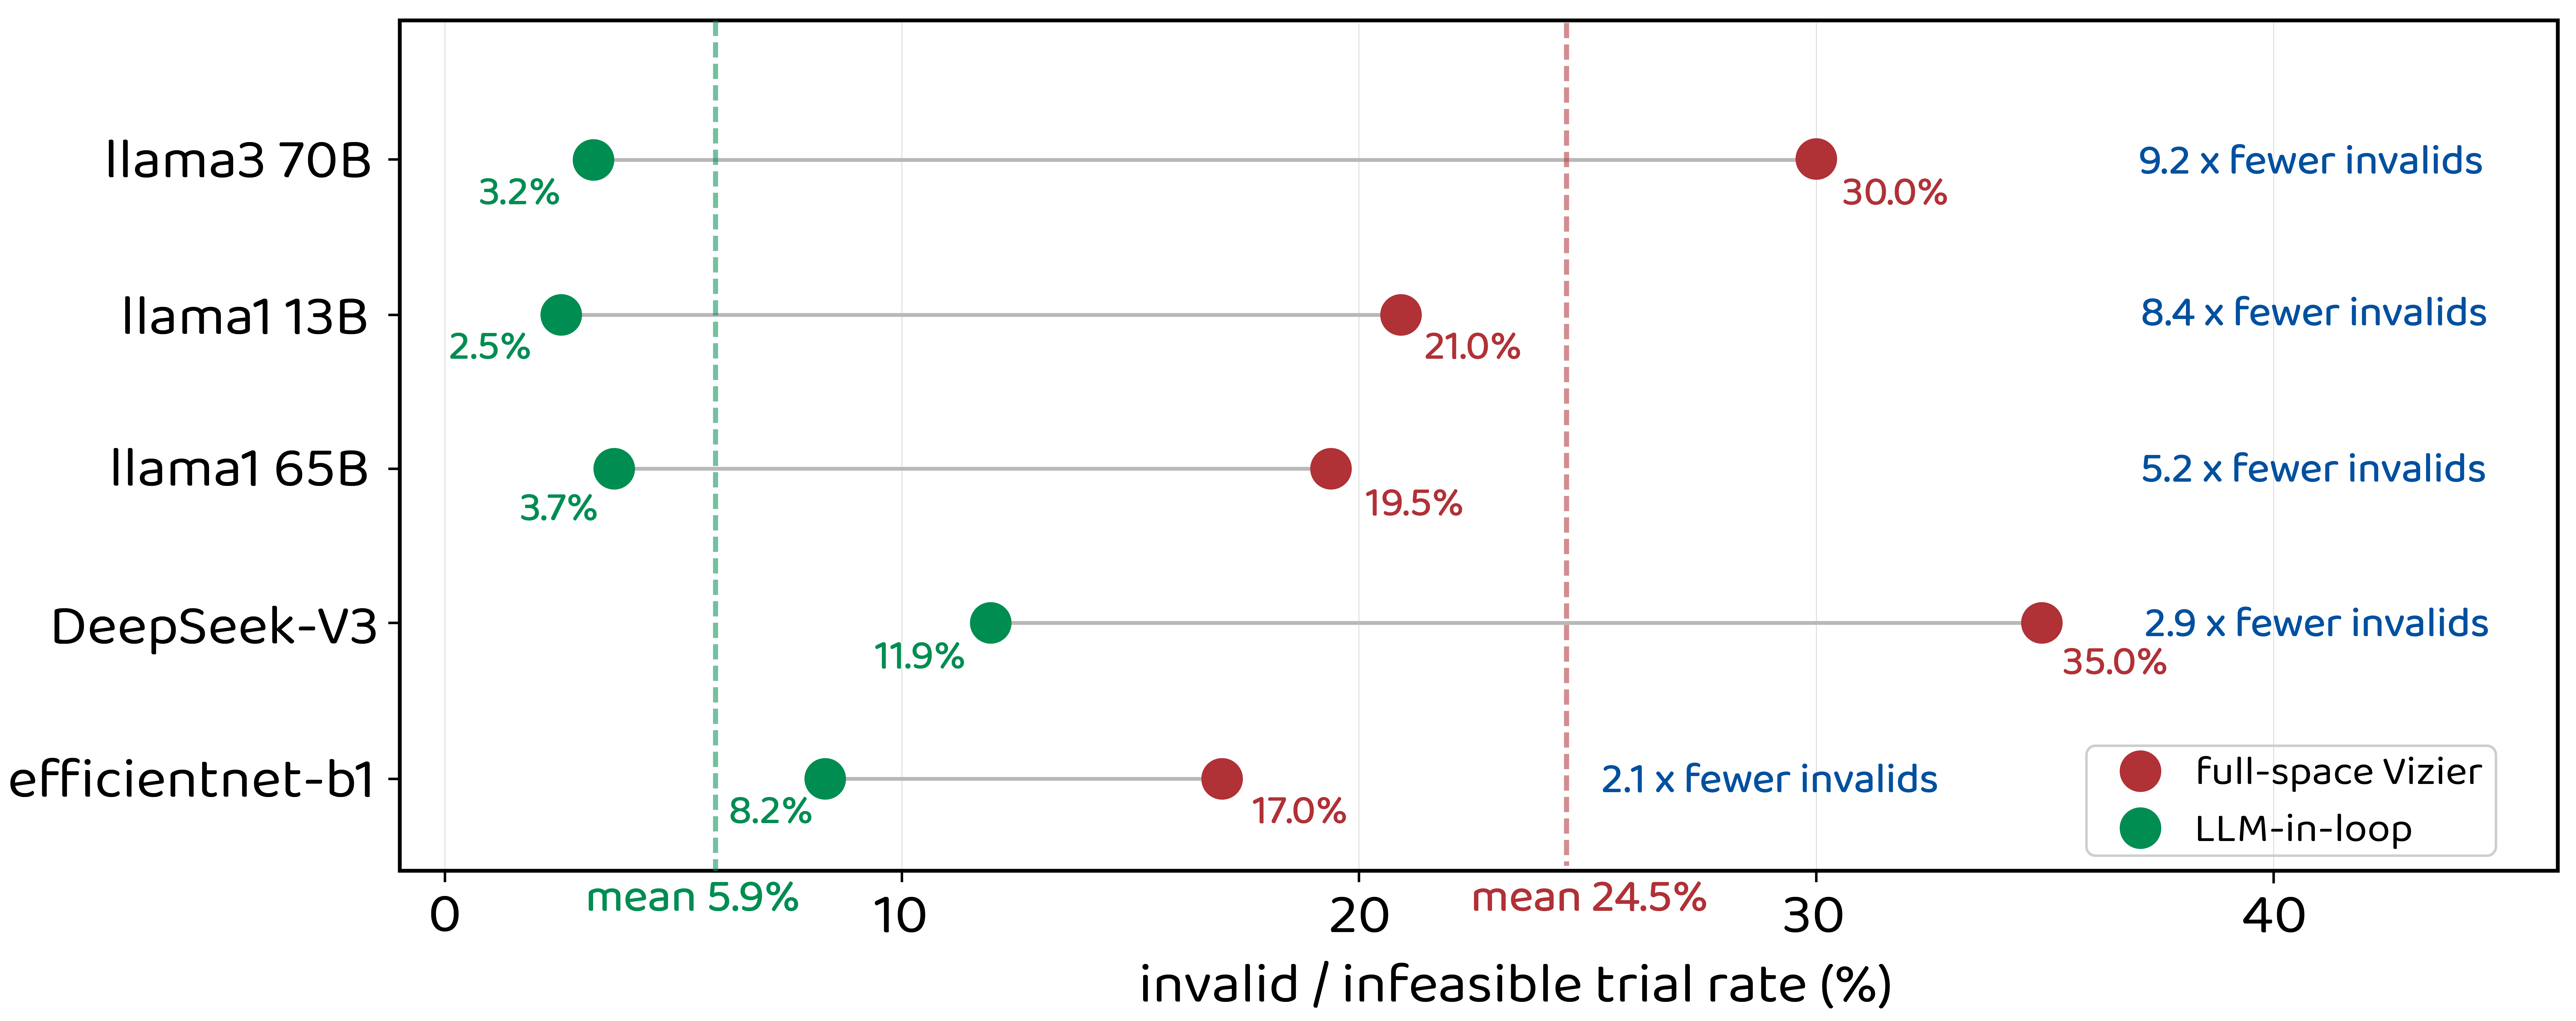
\includegraphics[width=0.85\linewidth]{fig3/llm_guide_v1.png}
% % % \caption{Strategic Intelligence vs. Stochastic Brute Force}\label{fig:llm}
% % % \end{figure}



% % % The LLM should not just ask, “What chip has the best Perf/TDP?” We aim to answer the question “Given this user’s workload and deployment goal, what is the architectural region to search for this deployment task?”. Therefore we have the LLM emit profile-conditioned campaigns that take specific user inference tasks into consideration. For each $(\text{deployment profile},\ \text{workload})$ cell, we ran a
% % % 200-trial LLM-Architect experiment using the same Qwen2.5-7B-Instruct + LoRA with differing user input profiles. At the start of each round, the prompt was assembled from a fixed system
% % % prompt, the active deployment profile, three few-shot examples, and a per-round user message containing the workload, recent feedback signals, current search bounds, and the causal ledger.
% % % The Strategist returned a one-line JSON campaign patch, which the
% % % validator accepted only if it was a strict legal subset of the parent space, satisfied hard rules such as patch-volume $\leq 10\%$, ridgepoint and MAC/BW constraints, and avoided forbidden regions.

% % % Thus, the experiment isolates whether the profile-conditioned LLM prompt alone can steer the same V1 evaluator toward different hardware families under different deployment intents.



% % % \todo{Compare convergence rate of LLM-guided hardware search vs.\ Vizier-only (Bayesian, LCS, random baselines) in the style of FAST Figure~11. Report:
% % % \begin{itemize}
% % %     \item Number of trials to reach $X\%$ of best Perf/TDP found by 5,000-trial Vizier
% % %     \item Quality of LLM-proposed configurations vs.\ Vizier-proposed configurations
% % %     \item Qualitative analysis of LLM reasoning about hardware bottlenecks
% % % \end{itemize}
% % % }

% % % \subsubsection{ROI Analysis}

% % % \todo{Update FAST's ROI analysis (Table~4) with the improved Perf/TDP numbers from FAST-CORGI. Report deployment volumes required to reach 1$\times$, 2$\times$, 4$\times$ ROI targets. If Perf/TDP improvements are larger than FAST's, the break-even deployment volume should decrease correspondingly.}

% % % \subsubsection{Pareto Frontier}

% % % \todo{Plot the Perf/TDP vs.\ area Pareto frontier for V1-optimized designs compared to FAST and TPU-v3 baseline, analogous to FAST Figure~12.}

% % page edit

% % \section{Experiments}
% % \label{sec:experiments}
% % In all cases we use an adapted JAX PDLP solver for large models at LLama70-B and DeepSeekv3 scale across all three methods (Static, CHEETAH-V0, CHEETAH-V1); and use HiGHS as the default solver for all other smaller neural network models. In order to be consistent with prior work, our experimental results are presented as orders of speedup / performance against a vanilla TPU-V3. This is also since TPUs are targeted for NN accelerators (as opposed to GPUs), and the TPU-V3 has the most information publically released, making it possible for us to simluate it more accurately. 

% % \subsection{Experimental Setup}

% % \paragraph{Static Sequential Baseline.}
% % We compare against the static optimization FAST framework using a simulated TPU-v3 baseline normalized to a sub-10nm process technology, following the same methodology as Zhang \etal. The baseline simulator is well-correlated with production hardware: on average within 8.2\,$\pm$\,2.7\% of profiled TPU-v3 performance. We evaluate against a \emph{simulated} TPU-v3 baseline to account for optimistic simulator assumptions.

% % We evaluate across 11 representative workloads: EfficientNet-B1 through EfficientNet-B7, Llama13, 65, 70 models, and DeepSeek-V3-MoE. These workloads stress different parts of the hardware design space: EfficientNet stresses low-operational-intensity depthwise convolutions, while Llama and DeepSeek stress memory capacity, bandwidth, and large matrix operations. 

% % \textbf{Single-workload specialization.} Each neural network workload is optimized independently. This experiment measures the best workload-specific hardware found under a fixed trial budget and identifies architectural preferences such as Global Memory size, bandwidth, MAC count, and systolic shape. In the case of Staitic and V0 methods, the pipeline involves: Vizier - Timeloop - LP solver. In the case of the V1 method, the pipeline is simplified to Vizier - LP solver. In each case we iterate for 100 trials per method x NN. 

% % % \textbf{Fixed-hardware-workload generalization.} We search for general-purpose datapaths that perform well across the workload suite. The objective is a harmonic or geometric aggregation of per-workload Perf/TDP, forcing the search to balance CNN-style memory pressure and LLM-style compute/memory trade-offs.

% % \textbf{LLM-Architect guides outer search.} We the LLM-guided outer-loop controller which proposes search-space interventions for Vizier. The advantage of the CHEETAH-V1 formulation is it removes dependence of Timeloop in the loop. Therefore the loop is reduced to just Vizier-LP solve, which dramatically speeds up the iterative process, thus permitting the LLM-Architect outer loop. The LLM is only permitted to change the search neighborhood of Vizier's input, the strict LP formulation on the inner loop does not change. This ensures mathematical and physical constraints are upheld in the space of co-design. 

% % % \paragraph{Optimization framework.}
% % % For the outer hardware search loop, we use Google Vizier with LCS optimization and safe search, running 100 trials per experiment (method X NN x Exp). Each trial invokes the LP solver for the inner optimization. The Static and V0 methods additionally have Timeloop in the loop (Vizier-Timeloop-LP solve). The advantage of the v1 formulation is it removes dependance of Timeloop in the loop. Therefore the loop is reduced to just Vizier-Lp solve, which dramatically speeds up the iterative process, thus permitted the Strategic LLM outer loop.

% % We validate our framework through a multi-level audit process to ensure physical and numerical rigor.
% % \textbf{Roofline Auditor.}
% % A deterministic Roofline Auditor enforces physical feasibility by
% % verifying that LP-predicted latencies never fall below the theoretical
% % bound
% % \begin{equation}
% %     \mathrm{LB} = \max\!\left(t_{\mathrm{compute}},\;
% %     t_{\mathrm{memory}}\right),
% %     \label{eq:roofline_lb_val}
% % \end{equation}
% % where $t_{\mathrm{compute}}$ and $t_{\mathrm{memory}}$ represent the
% % peak compute and memory bandwidth floors, respectively.
% % All reported V0/V1 results are roofline-feasible with valid
% % $\mathrm{MFU}_{\mathrm{bound}}$ and memory utilization metrics.

% % \textbf{Campaign Validator.}
% % A deterministic Campaign Validator legalizes LLM-proposed architectural
% % neighbourhoods by enforcing hard hardware constraints — including TDP
% % caps, area limits, and power-of-two parameter ranges — prior to Vizier
% % sampling.

% % \textbf{Causal Ledger.}
% % A Causal Ledger tracks LLM interventions and observed outcomes,
% % preventing redundant exploration of empirically invalid regions and
% % ensuring full auditability of the search loop.

% % \textbf{Solver Diagnostics.}
% % We monitor solver diagnostics including primal/dual residuals, duality
% % gap, and rounding gap. Designs are treated as trustworthy only when both
% % the continuous LP relaxation and the rounded integer solution are
% % numerically well-behaved.


% % \subsection{Main Results}

% % % \subsubsection{V0 vs.\ FAST Static Fusion}

% % % \todo{Insert results table and figure comparing V0 (time-indexed placement + rematerialization) against FAST's static fusion ILP on all benchmarks. Key metrics: Perf/TDP improvement, fusion efficiency (\% of DRAM stall time eliminated), rematerialization frequency (how often does the solver choose to recompute rather than reload?).}

% % % \paragraph{Expected findings.}
% % % V0's dynamic placement should show the largest gains on workloads with: (1)~tight Global Memory budgets where static pinning wastes capacity on tensors that are only needed briefly, (2)~long dependency chains where tensor lifetimes vary substantially, and (3)~cheap-to-recompute operations with large activations (\eg, depthwise convolutions in EfficientNet).

% % % \subsubsection{V1 vs.\ V0: Joint Tiling and Fusion}

% % % \todo{Insert results table and figure comparing V1 against V0 on all benchmarks. Key metrics: Perf/TDP improvement, number of operations where V1 selects a different tiling configuration than Timeloop's greedy choice, and the resulting compute efficiency vs.\ fusion trade-off.}

% % % \paragraph{Expected findings.}
% % % V1 should show the largest gains on architectures with highly diverse layer types where a single tiling configuration cannot serve all operations well. EfficientNet (depthwise + pointwise convolutions with 100$\times$ variation in working-set sizes) and hybrid CNN-transformer models (convolutions + attention + MLP with fundamentally different compute-memory profiles) are expected to benefit most.


% % % \subsubsection{stiatic vs v0 vs v1}
% % % \begin{figure}[ht!]
% % %     \centering
% % %     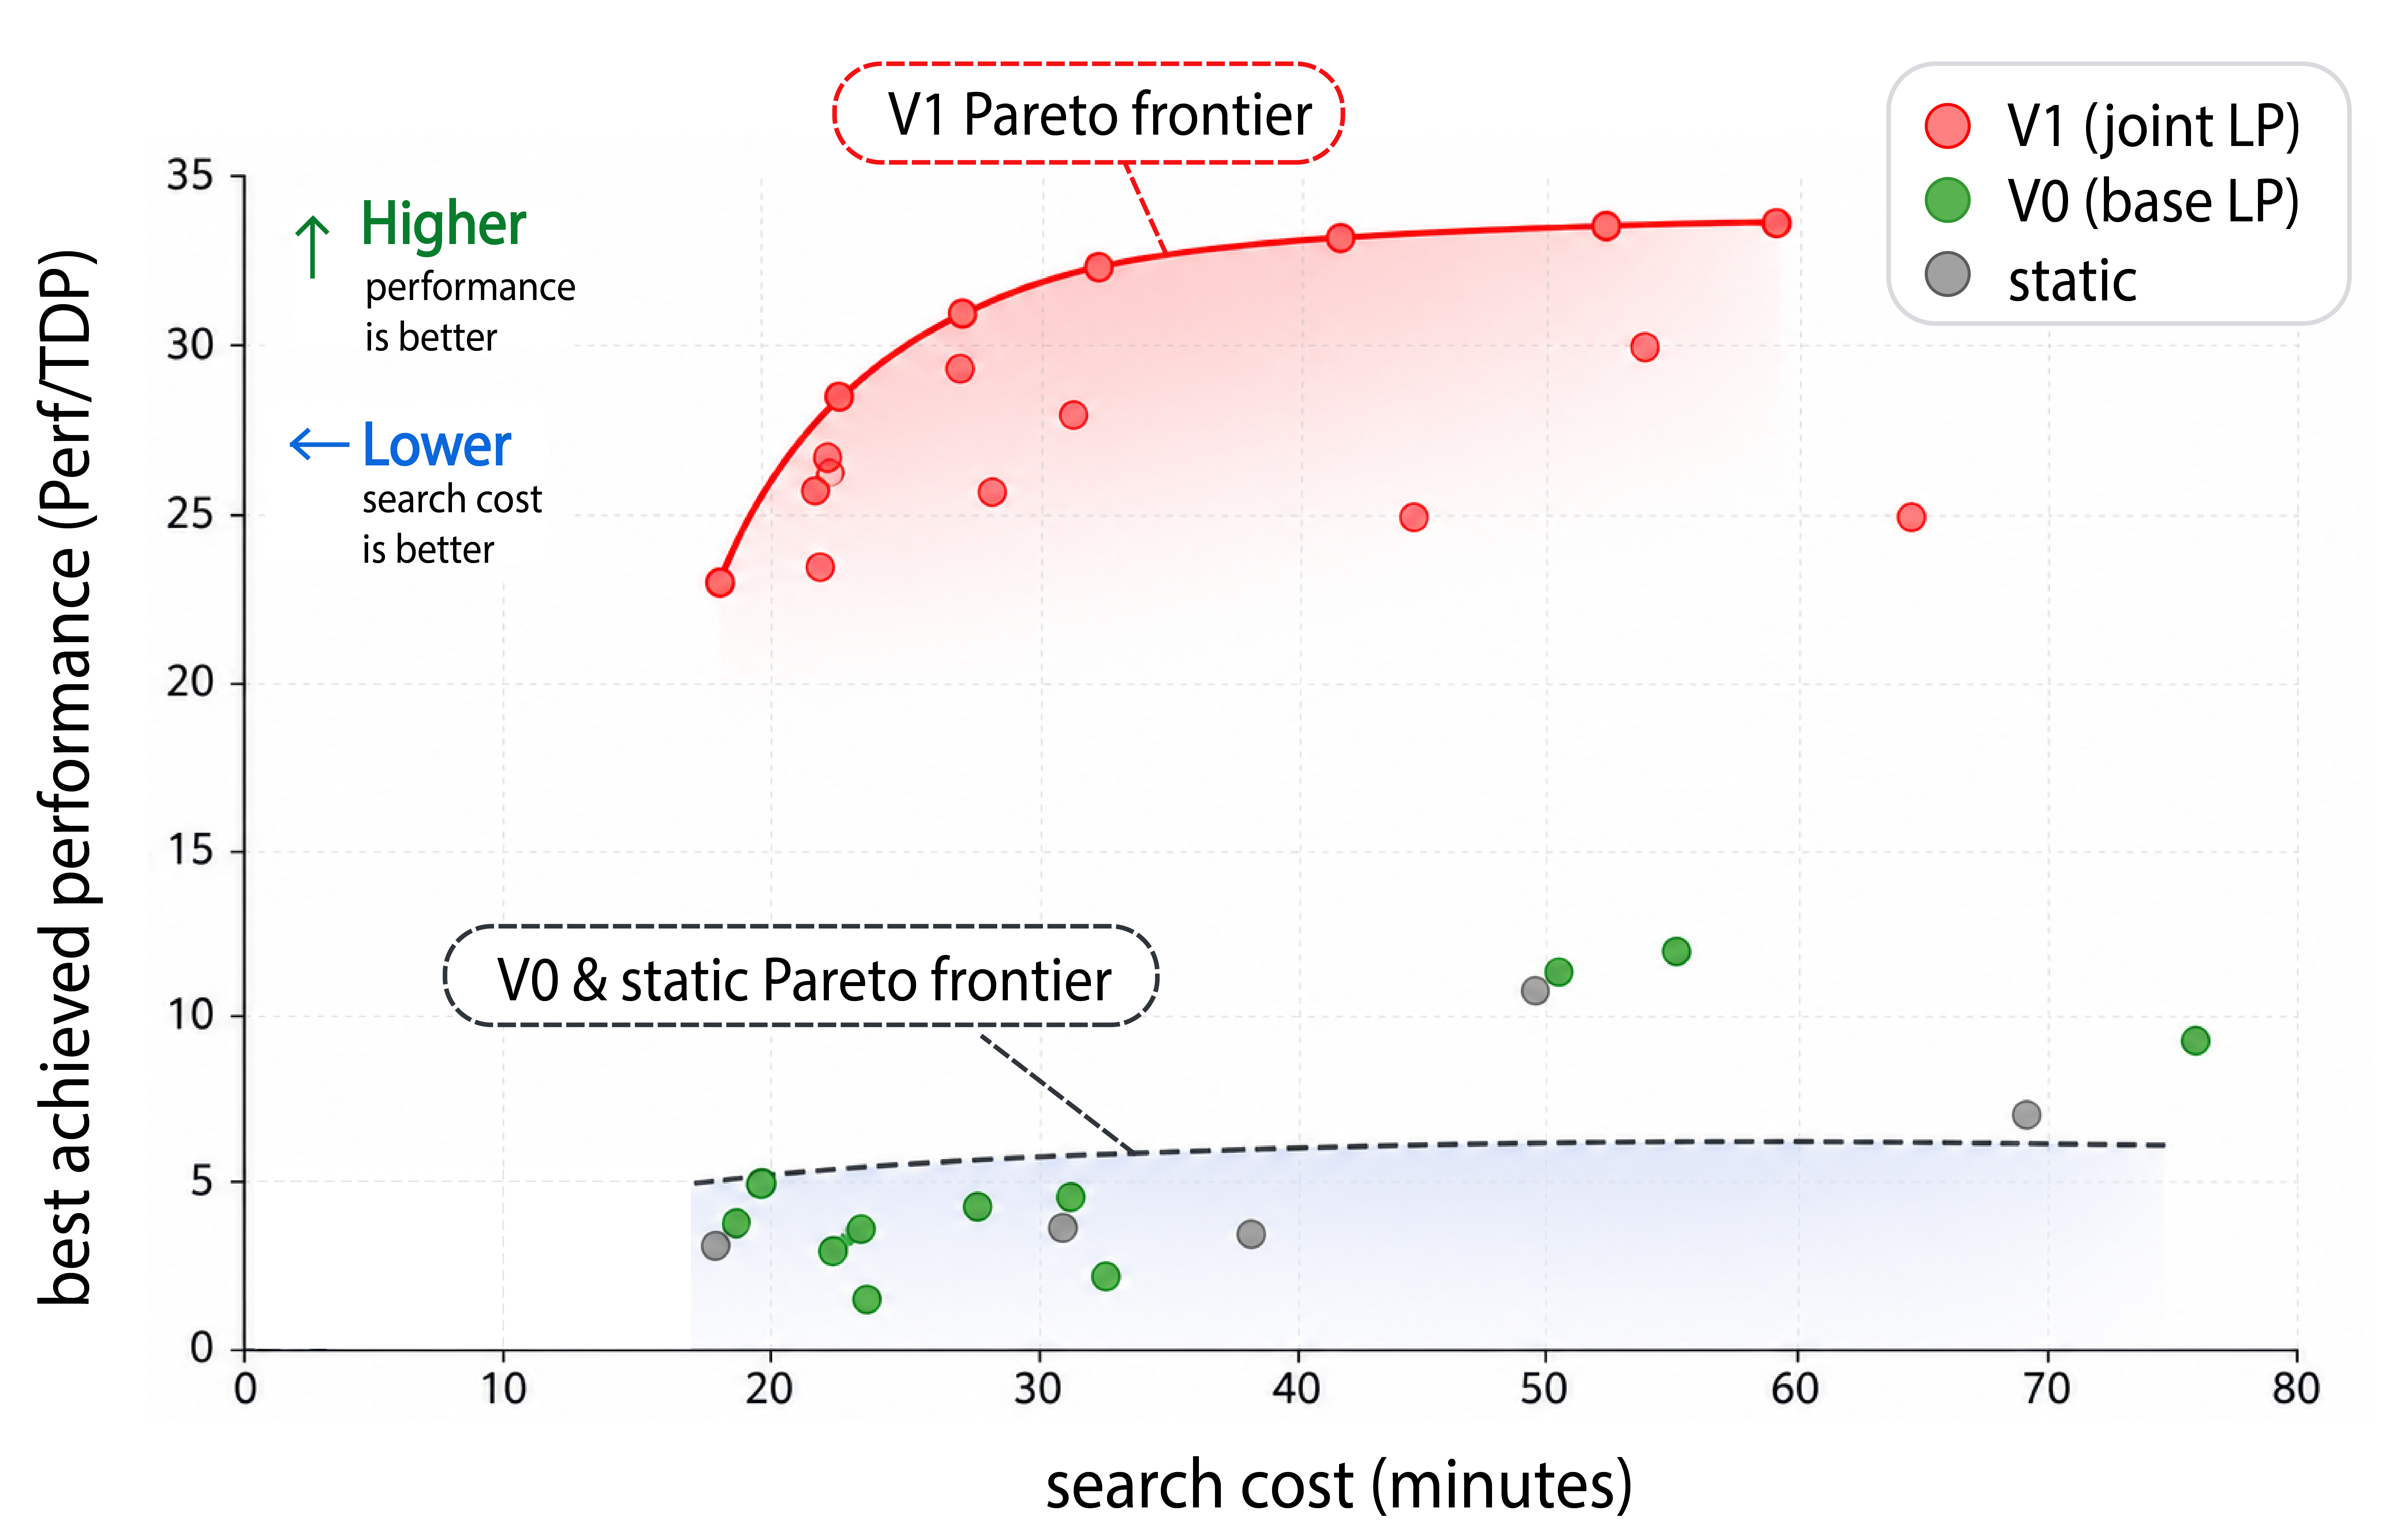
\includegraphics[width=0.7\linewidth]{figs/pareto_v2.png}
% % %     \caption{pareto frontier plot}
% % % \end{figure}
% % \begin{figure}[ht!]
% %     \centering
% % 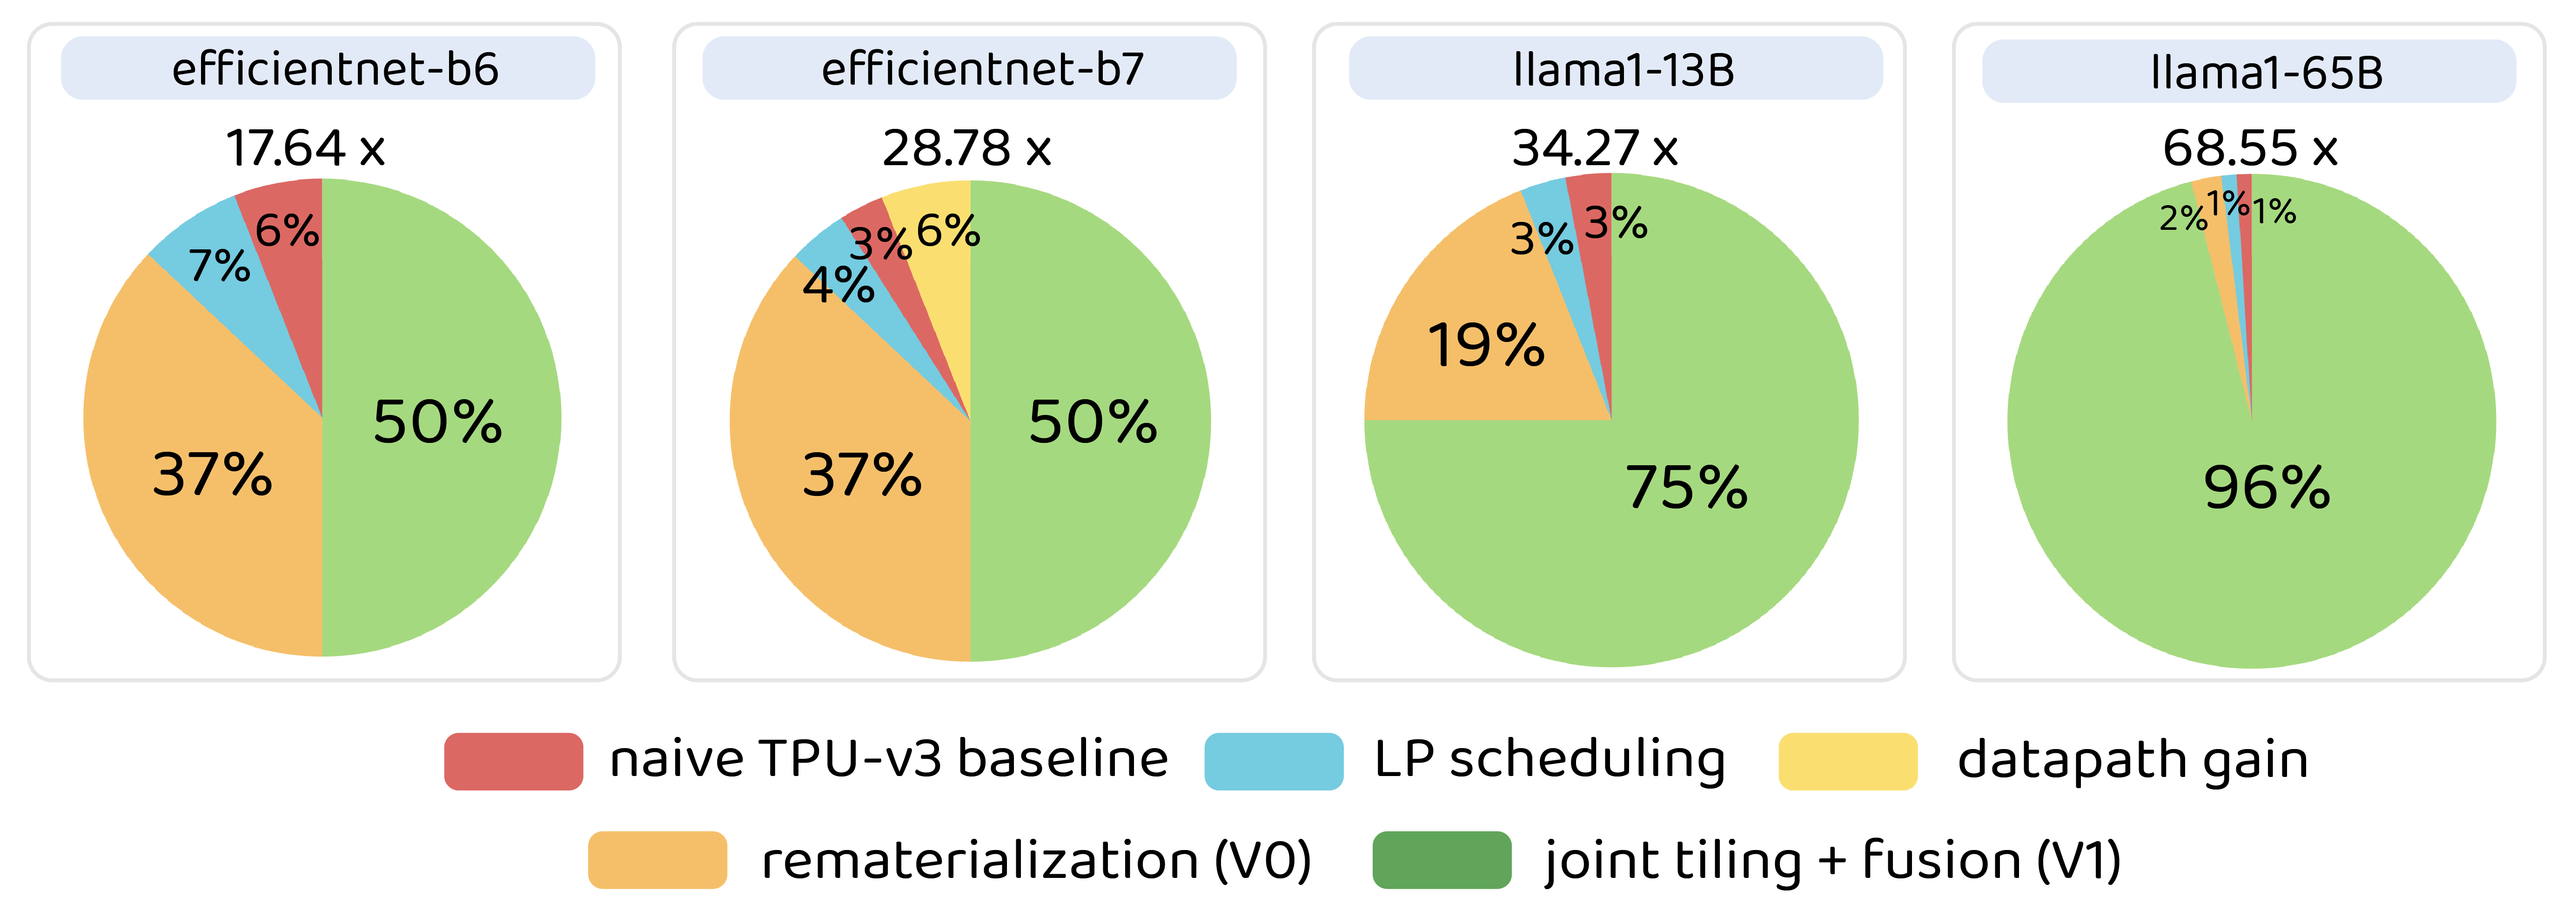
\includegraphics[width=0.85\linewidth]{fig3/speedup_decomposition_final_v2.png}
% % \caption{Speedup decomposition over naive TPU-v3 baseline. Each pie shows the 
% % relative contribution of four optimization sources to the total speedup. CHEETAH-V1 joint tiling + fusion dominates on all workloads, 
% % especially on larger models where memory management is the primary bottleneck.}\label{fig:accel_decompose}
% % \end{figure}
% % \subsubsection{Static Baseline vs.\ CHEETAH-V0 vs.\ CHEETAH-V1 Unlock Progressive Gains}


% % Figure~\ref{fig:accel_decompose} decomposes the total speedup over a naive TPU-v3 baseline into four sources: LP-based scheduling and fusion, datapath gain from hardware search, dynamic rematerialization (CHEETAH-V0), and joint tiling + fusion (CHEETAH-V1).

% % The dominant contributor across all workloads is V1's joint tiling-fusion 
% % optimization. On EfficientNet-B1, V1 accounts for 50\% of total speedup, 
% % with LP scheduling (28\%) and datapath gain (22\%) splitting the remainder---and 
% % no rematerialization benefit, consistent with B1's small activation footprint 
% % fitting comfortably in Global Memory. B3--B4 show a similar 50\% V1 share, but 
% % V0 rematerialization now contributes 25\%, reflecting the growing value of 
% % recomputing large depthwise activations rather than reloading them from DRAM. 
% % From B5 onward, V1's share rises sharply to 75--88\%, as the increasing 
% % model size makes joint tiling-fusion the primary lever: memory management 
% % dominates, and the remaining sources (LP scheduling, V0, datapath) each shrink 
% % to single-digit percentages. The same pattern holds on Llama, where V1 accounts 
% % for 83--87\% of the total speedup.

% % % \begin{wrapfigure}{r}{0.48\textwidth}
% % %     \centering
% % %     \vspace{-12pt}
% % %     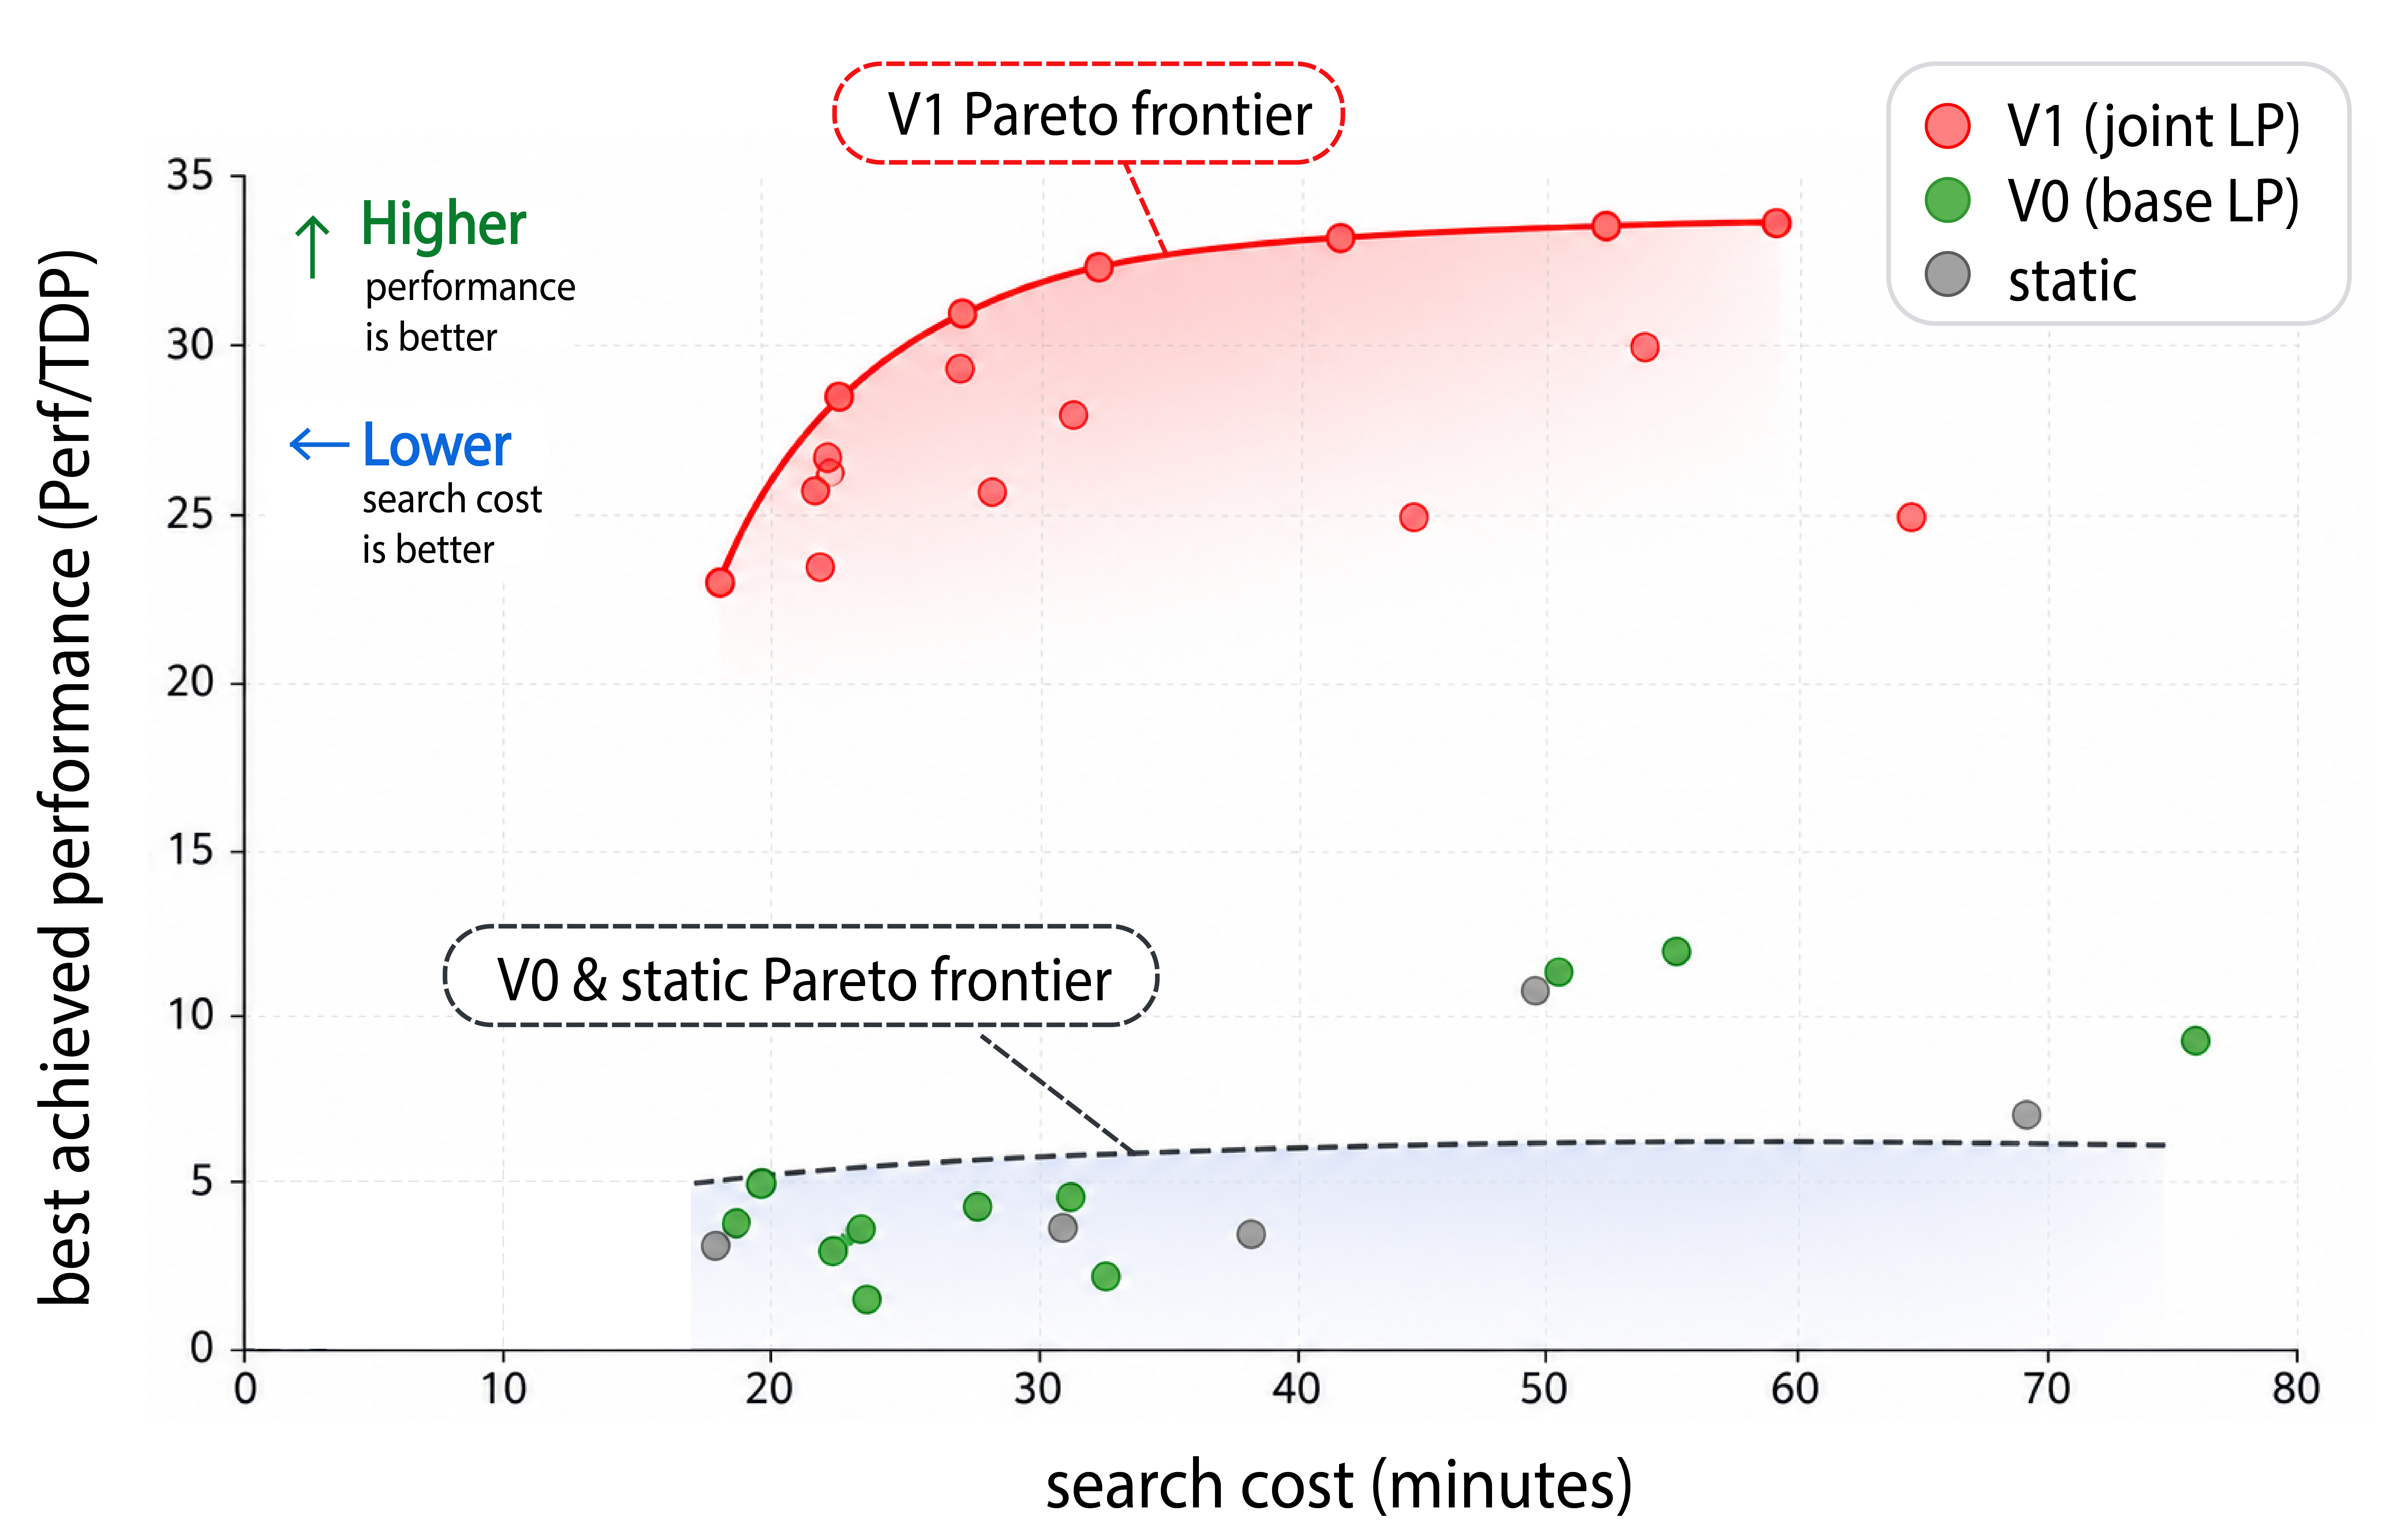
\includegraphics[width=0.48\textwidth]{figs/pareto_v2.png}
% % %     \vspace{-18pt}
% % %     \caption{Search cost vs.\ Perf/TDP Pareto frontier. V1 dominates V0 and static across all time budgets.}
% % %     \label{fig:pareto}
% % %     \vspace{-10pt}
% % % \end{wrapfigure}

% % Critically, Figure~\ref{fig:speedup} shows static fusion method is \emph{infeasible} on modern large models (Llama-70B, and DeepSeek-V3), because their large activation tensors cannot fit under a static pinning policy. The V0 formulation resolves feasibility for on large models via dynamic placement but remains time-intensive for a small number of 50 trials: measuring 58.42 hours on Llama-70B and 69.39 hours on DeepSeek-V3 (Figure~\ref{fig:wallclock}). In contrast Figures~\ref{fig:wallclock} and ~\ref{fig:speedup}, show the CHEETAH-V1 formulation out performs comparitive strategies in terms of speedup against the TPU-V3 baseline, and require only 1.17 hours on Llama-70B and 2.17 hours on DeepSeekv3 for 50 trails---a ${\sim}93\%$ average reduction. The powerful joint formulation is able to select memory-efficient tiling configurations alongside placement, achieving feasibility across the entire workload suite, demonstrating that joint optimization is not merely an incremental improvement but a qualitative capability unlock for large-scale models.

% % % This demonstrates that by exploiting structural invariance and GPU-accelerated mathematical optimization, CHEETAH-V1 reduces the end-to-end co-design search time from days to under 2.2 hours—a ${\sim}93\%$ average reduction—while discovering architectural points that deliver up to $35\times$ speedup over the TPU-v3 baseline.

% % % Figure~\ref{fig:pareto} shows the Pareto frontier of best-achieved Perf/TDP versus wall-clock search cost. V1 strictly dominates both V0 and static at every time budget: within 10 minutes of search, V1 already exceeds the best Perf/TDP that V0 or static achieve after 60+ minutes. The V1 Pareto frontier reaches ${\sim}35\times$ Perf/TDP, roughly $3\times$ higher than the V0/static frontier at ${\sim}10\text{--}12\times$. This gap reflects two compounding advantages: V1 explores a strictly larger feasible region (joint tiling-fusion), and it eliminates Timeloop from the per-trial critical path, allowing more trials within any fixed time budget.



% % \paragraph{Practical insight.}
% % Both LPs are extreme-aspect-ratio sparse: for \texttt{llama3\_70b},
% % $m, n \sim 10^6$ and $\mathrm{nnz} \sim 5 \times 10^6$, giving roughly
% % 1 nonzero per million matrix entries.
% % The time-band structure means a coordinate-descent or stochastic PDHG
% % solver would converge in $\mathcal{O}(T)$ sweeps if bands were the only
% % structure.
% % The capacity rows in both V0 and V1 LP formulations are the sole feature breaking strict banded structure, and they are precisely what couples the schedule globally. This is the desired behavior of a memory-aware placement formulation.

% % % \todo{Report LP solve times for V0 and V1 across all benchmarks. Compare wall-clock time per trial against FAST's SCIP-based ILP solver (20 min timeout). Report LP relaxation gap: how often do fractional solutions need integer rounding, and what is the quality loss from rounding?}

% % \paragraph{Structural invariance.}
% % For a fixed workload and LP formulation, the LP constraint matrix
% % has an invariant sparsity pattern across trials: the row/column
% % dimensions and nonzero locations are determined only by the model graph structure — layer count $L$, timestep count $T$, edge set $E$, and Pareto count $C$ — not by the hardware candidate.
% % Vizier changes only numerical values such as cycle coefficients,
% % memory-capacity bounds, bandwidth-scaled access costs, objective weights, and TDP/area parameters. 
% % This invariance allows us to reuse the same sparse matrix structure,
% % variable ordering, block layout, and JIT-compiled sparse kernels in our adapted JAX PDLP solver across all hardware trials for a given workload.

% % Numerically, we apply the same diagonal preconditioning pipeline
% % on each trial: a structural presolve with 20 log-geomean Ruiz iterations, followed by the PDLP preprocessing stack with 10 infinity-norm Ruiz iterations and one Pock--Chambolle $\ell_1$-scaling pass. This two-stage diagonal scaling handles the mixed coefficient magnitudes present in V0/V1 matrices — large byte-valued capacity rows together with $\pm 1$ persistence rows — without requiring a fragile matrix factorization.

% % In production, this preconditioning pipeline is reused structurally across trials, recomputes only cheap diagonal scalings, finishes in under one second for matrices with approximately $5 \times 10^6$ nonzeros, and avoids factorization failures entirely because it consists only of $D_1 A D_2$ arithmetic.

% % \subsubsection{LLM Architect vs. Optimizer}
% % The LLM Architect framework is modeled on SkyDiscover, and efficiently prunes the large outer hardware search loop by proposing campaign patches. Rather than predicting performance, the Architect reads a compact Causal Ledger containing invalid-rate history, MFU, roofline lower-bound checks, and LP diagnostics, then proposes a constrained hardware neighborhood for Vizier to search locally. The V1 LP remains the sole performance evaluator: for each candidate, it solves the joint tiling, fusion, placement, and rematerialization LP, while a deterministic Roofline Auditor rejects physically impossible results. In the widened V1 search space, all methods reach the same capped V1 Perf/TDP ceiling, so the key differentiator is search efficiency. The LLM loop reduces invalid hardware evaluations from 24.5\% under full-space Vizier to 5.9\% on average across five workloads, a 4.1× reduction in wasted trials, while preserving the same best V1 score. This shows that the LLM’s contribution is not replacing Vizier or the solver, but steering Bayesian optimization toward feasible, workload-appropriate architectural neighborhoods with far less wasted trials. This also sets the foundation for future work, where the LLM in the loop can adhere to follow more complex human reasoning signals.
% % \begin{figure}[ht!]
% %     \centering
% % 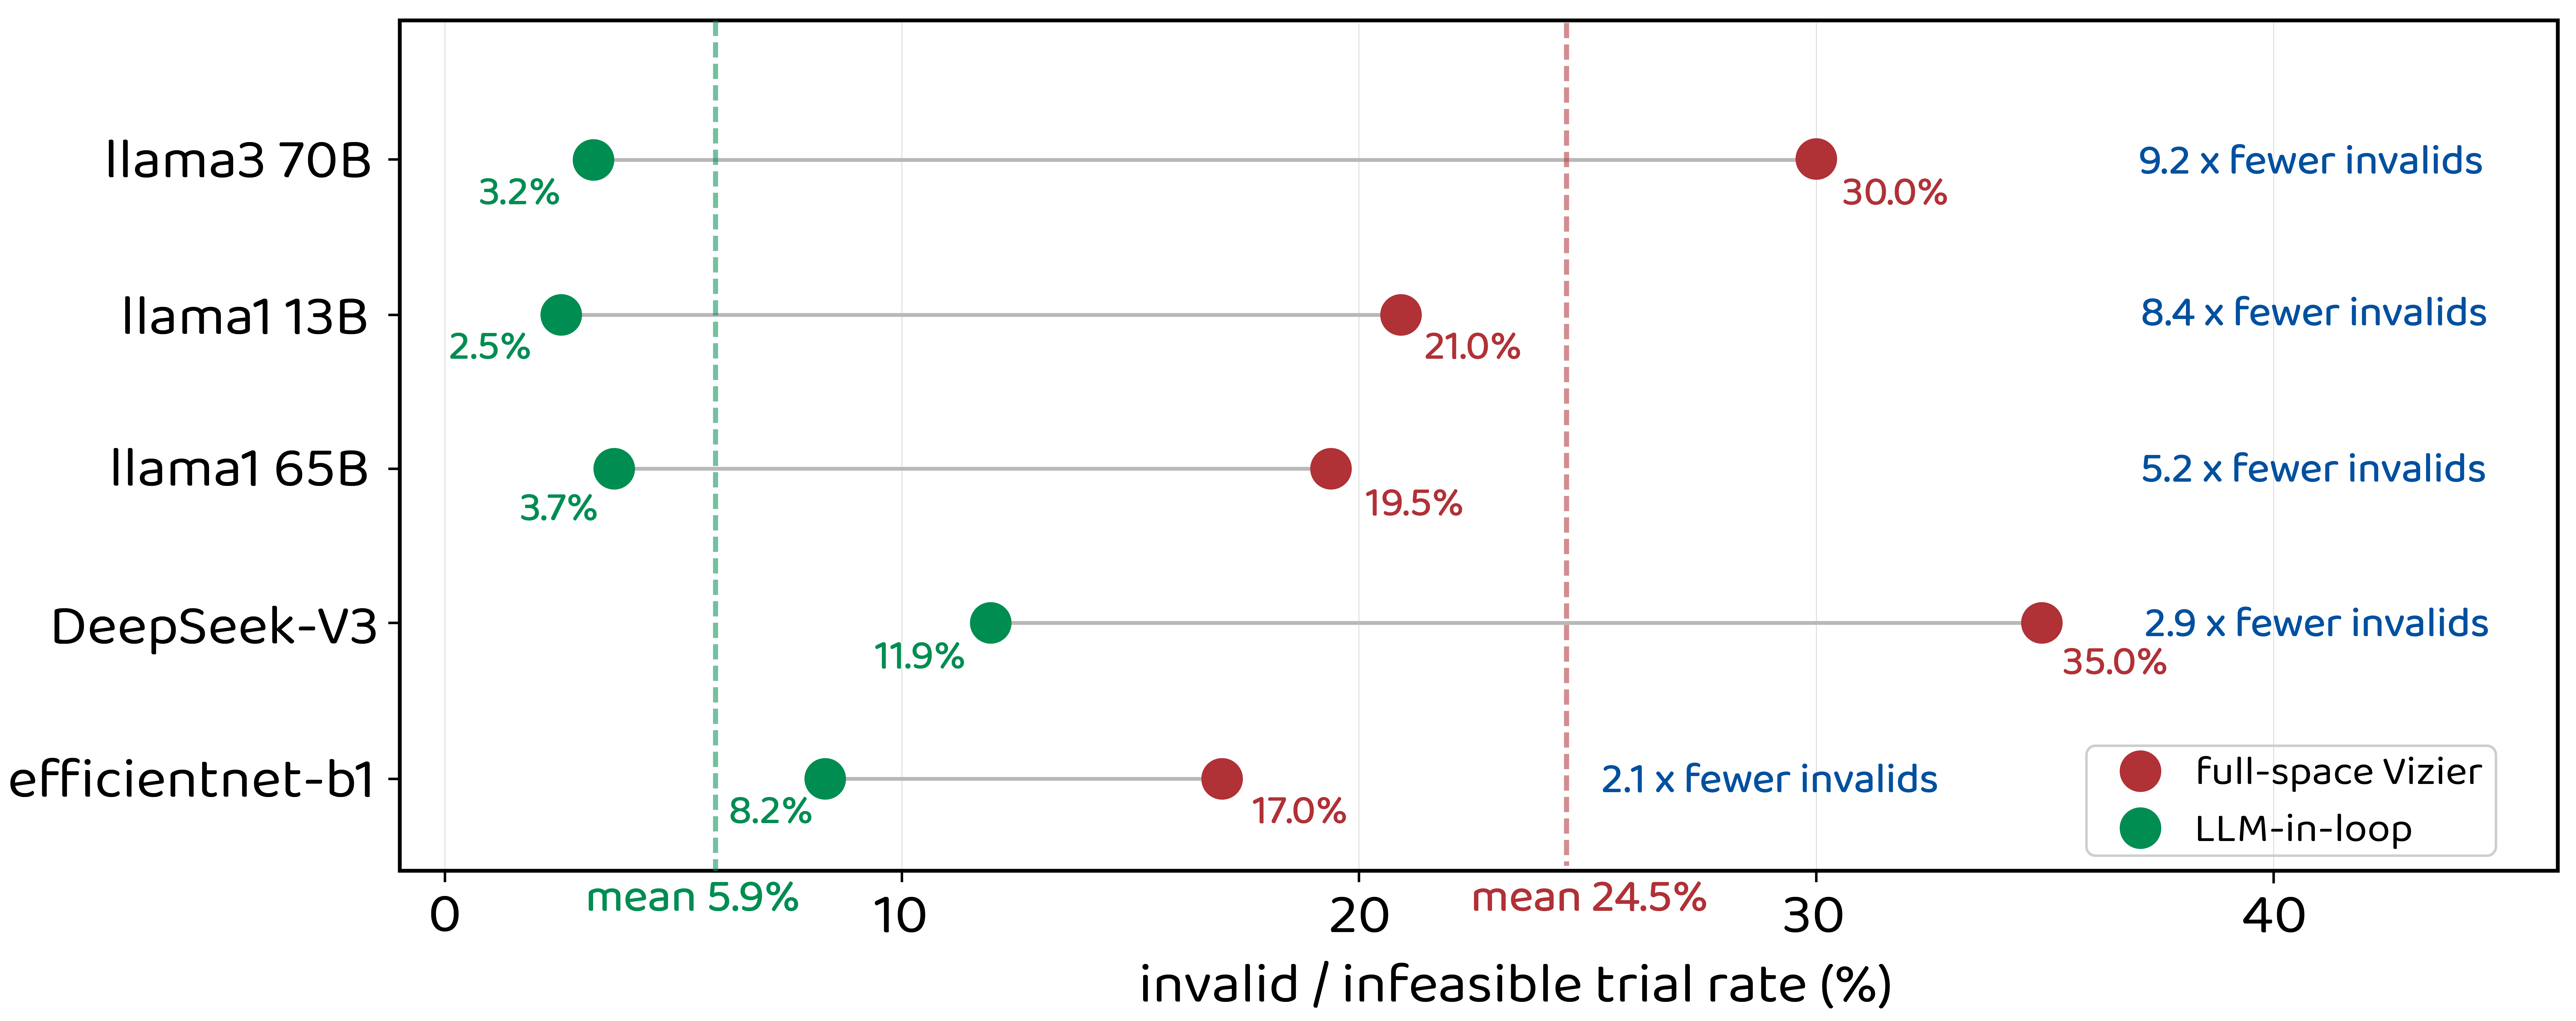
\includegraphics[width=0.85\linewidth]{fig3/llm_guide_v1.png}
% % \caption{Strategic Intelligence vs. Stochastic Brute Force}\label{fig:llm}
% % \end{figure}



% % % The LLM should not just ask, “What chip has the best Perf/TDP?” We aim to answer the question “Given this user’s workload and deployment goal, what is the architectural region to search for this deployment task?”. Therefore we have the LLM emit profile-conditioned campaigns that take specific user inference tasks into consideration. For each $(\text{deployment profile},\ \text{workload})$ cell, we ran a
% % % 200-trial LLM-Architect experiment using the same Qwen2.5-7B-Instruct + LoRA with differing user input profiles. At the start of each round, the prompt was assembled from a fixed system
% % % prompt, the active deployment profile, three few-shot examples, and a per-round user message containing the workload, recent feedback signals, current search bounds, and the causal ledger.
% % % The Strategist returned a one-line JSON campaign patch, which the
% % % validator accepted only if it was a strict legal subset of the parent space, satisfied hard rules such as patch-volume $\leq 10\%$, ridgepoint and MAC/BW constraints, and avoided forbidden regions.

% % % Thus, the experiment isolates whether the profile-conditioned LLM prompt alone can steer the same V1 evaluator toward different hardware families under different deployment intents.



% % % \todo{Compare convergence rate of LLM-guided hardware search vs.\ Vizier-only (Bayesian, LCS, random baselines) in the style of FAST Figure~11. Report:
% % % \begin{itemize}
% % %     \item Number of trials to reach $X\%$ of best Perf/TDP found by 5,000-trial Vizier
% % %     \item Quality of LLM-proposed configurations vs.\ Vizier-proposed configurations
% % %     \item Qualitative analysis of LLM reasoning about hardware bottlenecks
% % % \end{itemize}
% % % }

% % % \subsubsection{ROI Analysis}

% % % \todo{Update FAST's ROI analysis (Table~4) with the improved Perf/TDP numbers from FAST-CORGI. Report deployment volumes required to reach 1$\times$, 2$\times$, 4$\times$ ROI targets. If Perf/TDP improvements are larger than FAST's, the break-even deployment volume should decrease correspondingly.}

% % % \subsubsection{Pareto Frontier}

% % % \todo{Plot the Perf/TDP vs.\ area Pareto frontier for V1-optimized designs compared to FAST and TPU-v3 baseline, analogous to FAST Figure~12.}


% % edit for page limit
% \vspace{-0.3cm}
% \section{Experiments}
% \label{sec:experiments}
% \vspace{-0.2cm}
% \subsection{Experimental Setup}
% \vspace{-0.2cm}
% We compare against the FAST framework~\citep{zhang_fast} using a simulated TPU-v3 \citep{jouppi2021ten} baseline normalized to sub-10nm process technology (within $8.2 \pm 2.7\%$ of profiled TPU-v3 performance). We use an adapted JAX PDLP solver for large models (Llama-70B, DeepSeek-V3) and HiGHS \citep{huangfu2018parallel} for smaller models, reporting speedup over the TPU-v3 baseline consistent with prior work.
% We evaluate across 11 workloads: EfficientNet-B1 \citep{tan2019efficientnet} through B7 (stressing low-intensity depthwise convolutions), Llama-1 13B/65B and Llama-3 70B \citep{llama3modelcard}, and DeepSeek-V3-MoE \citep{deepseekv3report} (stressing memory capacity and bandwidth). Each workload is optimized independently under 100 trials per method. For Static and V0, the pipeline is Vizier$\to$Timeloop$\to$LP; for V1, it simplifies to Vizier$\to$LP. The LLM Architect outer loop proposes search-space interventions for Vizier; it is only permitted to change Vizier's search neighborhood while the strict LP inner loop remains unchanged.
% We validate all results through a multi-level audit process---Roofline Auditor, Campaign Validator, Causal Ledger, and solver diagnostics---as described in Section~\ref{sec:llm_outer} and detailed in Appendix~\ref{app:validation} and ~\ref{app:mfu}. All reported V0/V1 results are roofline-feasible with zero lower-bound violations.


% % \subsection{Main Results}

% % \subsubsection{V0 vs.\ FAST Static Fusion}

% % \todo{Insert results table and figure comparing V0 (time-indexed placement + rematerialization) against FAST's static fusion ILP on all benchmarks. Key metrics: Perf/TDP improvement, fusion efficiency (\% of DRAM stall time eliminated), rematerialization frequency (how often does the solver choose to recompute rather than reload?).}

% % \paragraph{Expected findings.}
% % V0's dynamic placement should show the largest gains on workloads with: (1)~tight Global Memory budgets where static pinning wastes capacity on tensors that are only needed briefly, (2)~long dependency chains where tensor lifetimes vary substantially, and (3)~cheap-to-recompute operations with large activations (\eg, depthwise convolutions in EfficientNet).

% % \subsubsection{V1 vs.\ V0: Joint Tiling and Fusion}

% % \todo{Insert results table and figure comparing V1 against V0 on all benchmarks. Key metrics: Perf/TDP improvement, number of operations where V1 selects a different tiling configuration than Timeloop's greedy choice, and the resulting compute efficiency vs.\ fusion trade-off.}

% % \paragraph{Expected findings.}
% % V1 should show the largest gains on architectures with highly diverse layer types where a single tiling configuration cannot serve all operations well. EfficientNet (depthwise + pointwise convolutions with 100$\times$ variation in working-set sizes) and hybrid CNN-transformer models (convolutions + attention + MLP with fundamentally different compute-memory profiles) are expected to benefit most.


% % \subsubsection{stiatic vs v0 vs v1}
% % \begin{figure}[ht!]
% %     \centering
% %     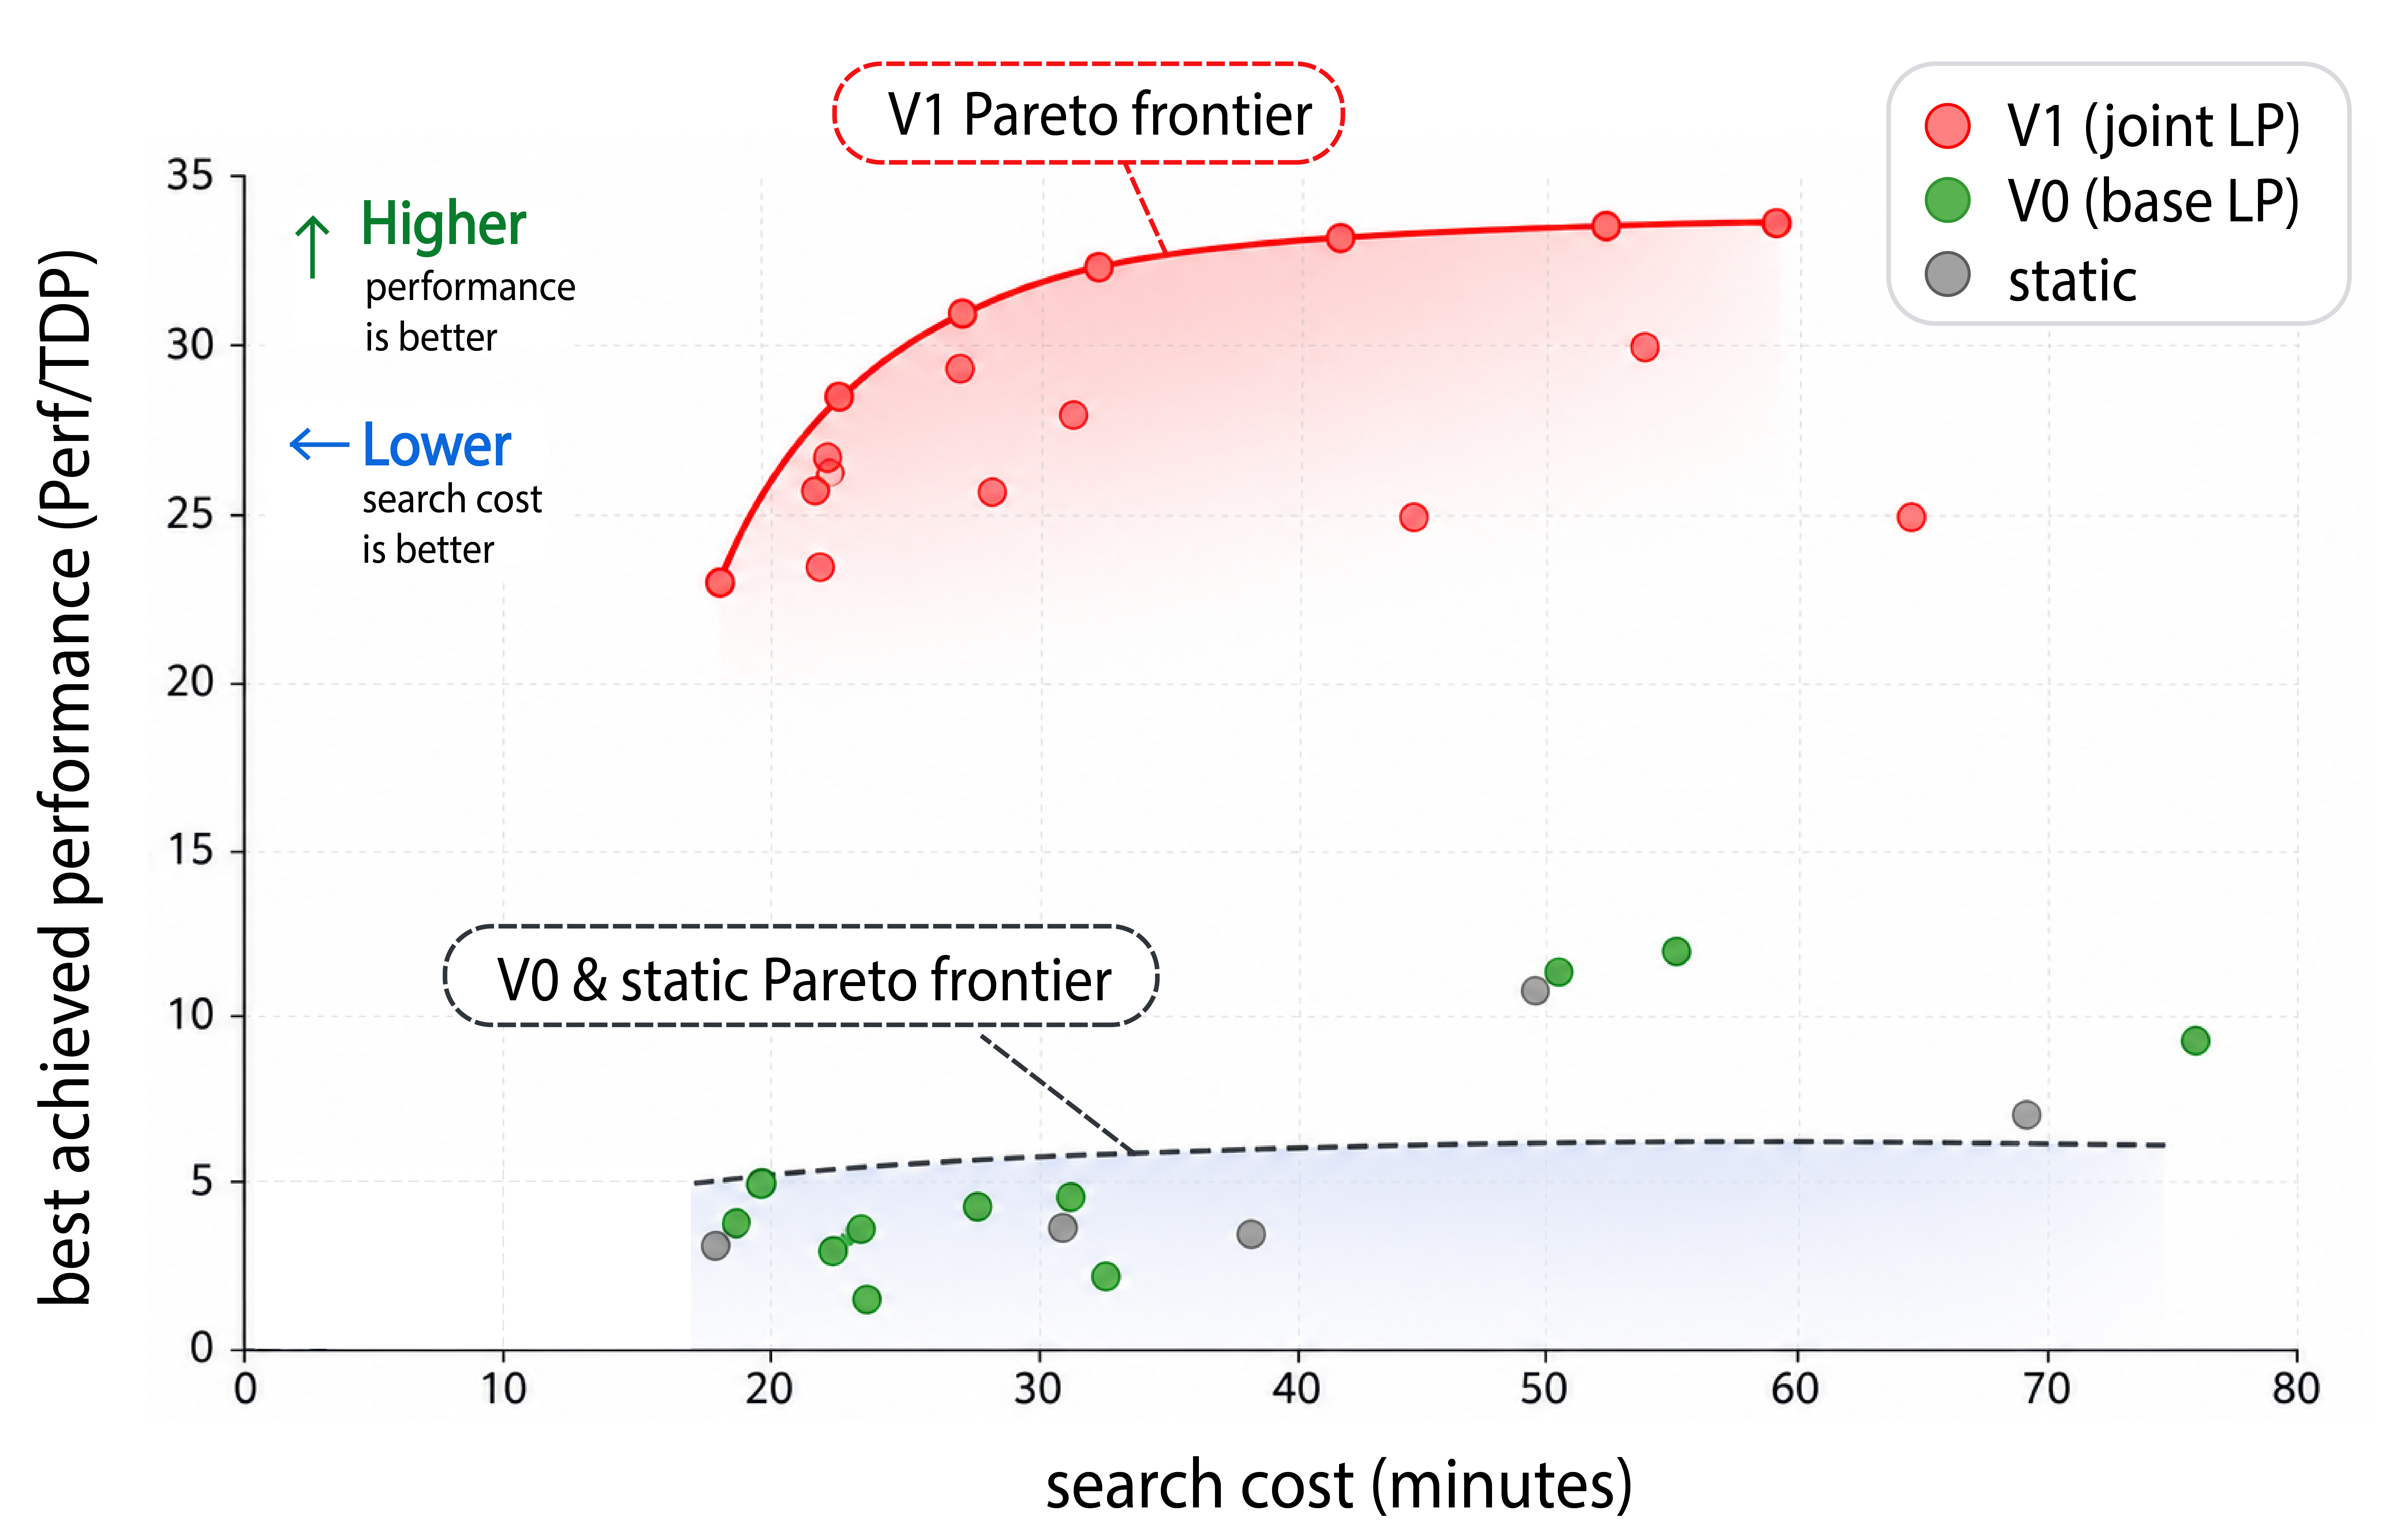
\includegraphics[width=0.7\linewidth]{figs/pareto_v2.png}
% %     \caption{pareto frontier plot}
% % \end{figure}
% \begin{figure}[ht!]
%     \centering
% 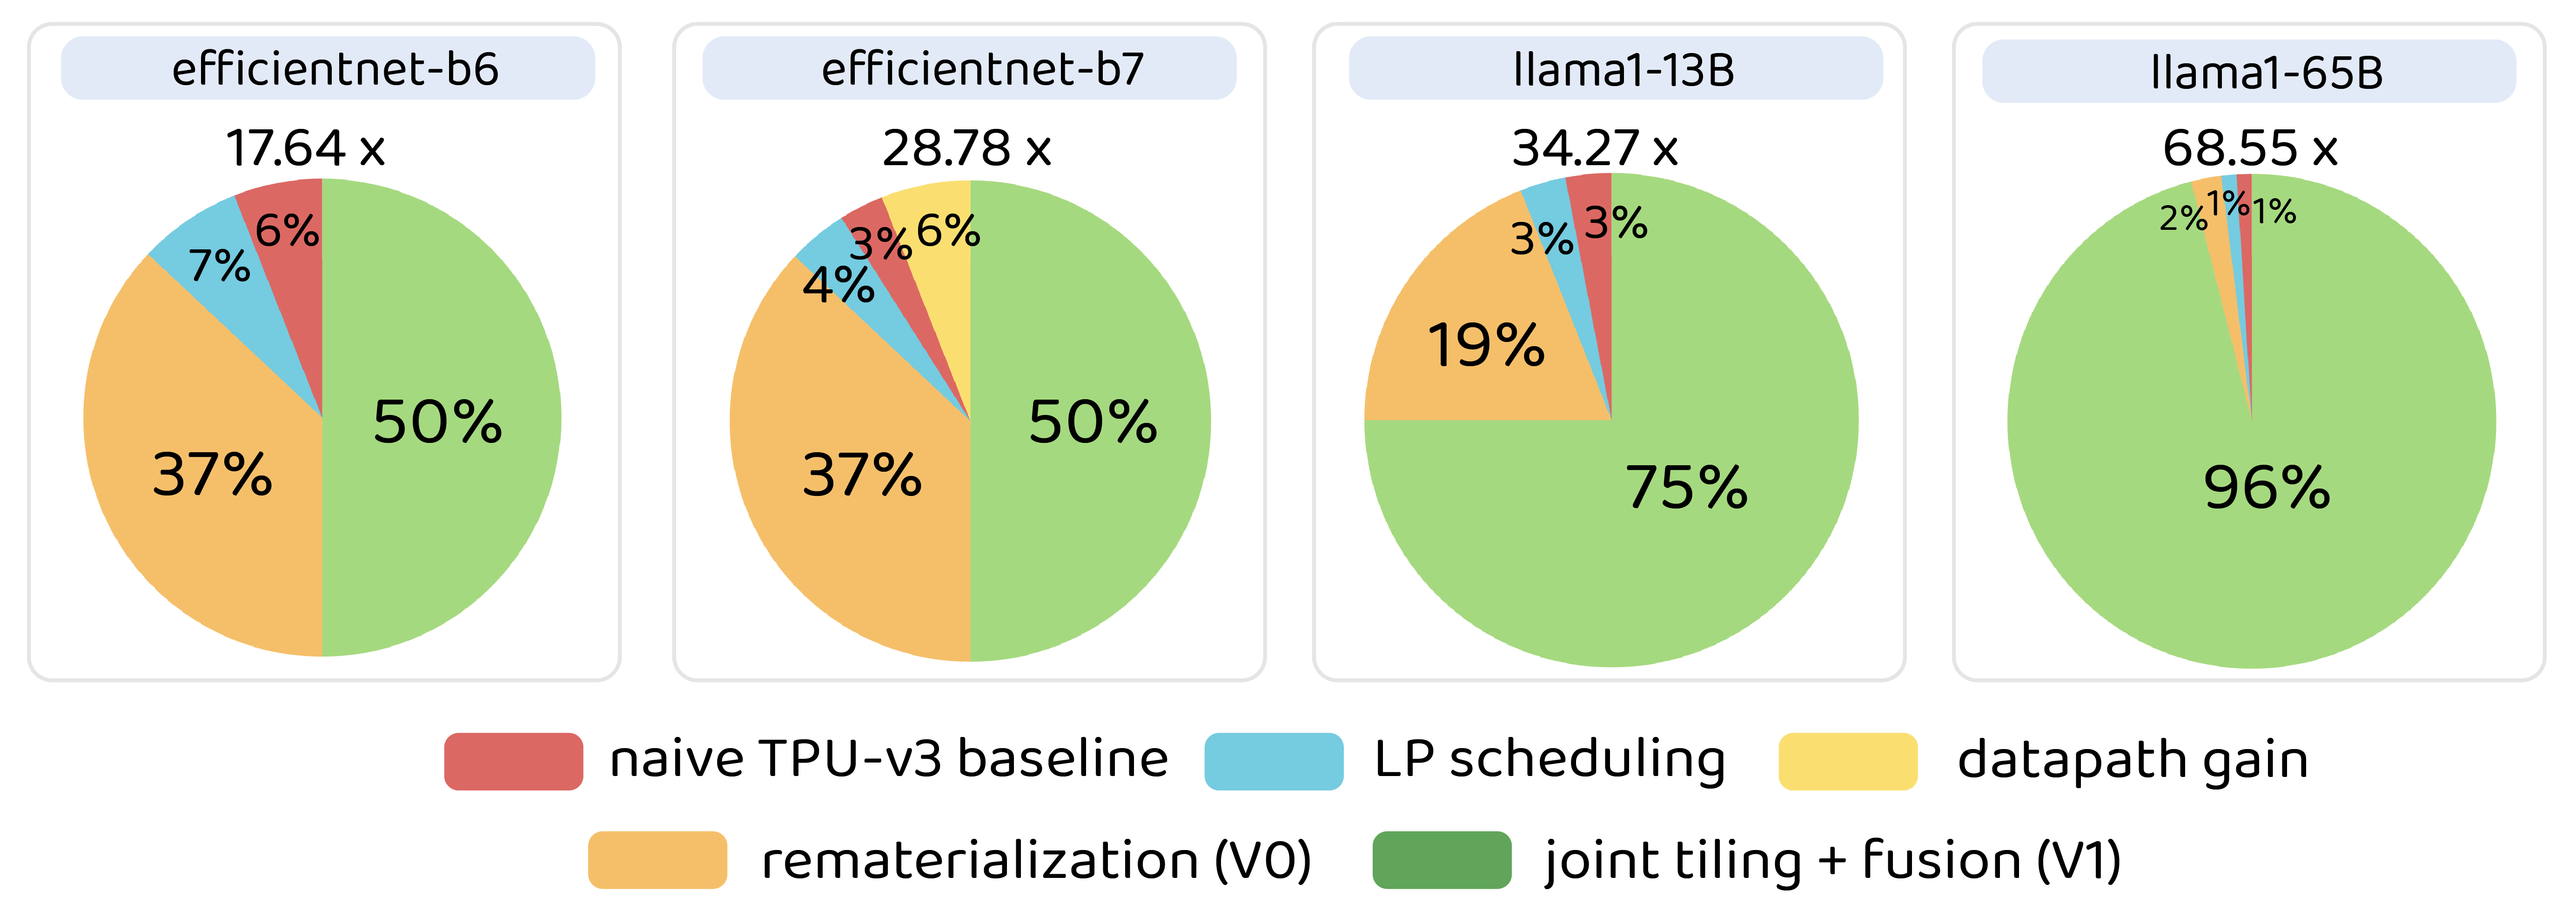
\includegraphics[width=0.85\linewidth]{fig3/speedup_decomposition_final_v2.png}
% \caption{Speedup decomposition over naive TPU-v3 baseline. Each pie shows the 
% relative contribution of four optimization sources to the total speedup. CHEETAH-V1 joint tiling + fusion dominates on all workloads, 
% especially on larger models where memory management is the primary bottleneck.}\label{fig:accel_decompose}
% \end{figure}
% \subsection{Static Baseline vs.\ CHEETAH-V0 vs.\ CHEETAH-V1 Unlock Progressive Gains}


% Figure~\ref{fig:accel_decompose} decomposes the total speedup over a naive TPU-v3 baseline into four sources: LP-based scheduling and fusion, datapath gain from hardware search, dynamic rematerialization (CHEETAH-V0), and joint tiling + fusion (CHEETAH-V1). Table~\ref{tab:LP_struct} gives side by side structural comparison of the V0 and V1 formulation matrices in greater detail. 

% The dominant contributor across all workloads is V1's joint tiling-fusion 
% optimization. On EfficientNet-B1, V1 accounts for 50\% of total speedup, 
% with LP scheduling (28\%) and datapath gain (22\%) splitting the remainder---and 
% no rematerialization benefit, consistent with B1's small activation footprint 
% fitting comfortably in Global Memory. B3--B4 show a similar 50\% V1 share, but 
% V0 rematerialization now contributes 25\%, reflecting the growing value of 
% recomputing large depthwise activations rather than reloading them from DRAM. 
% From B5 onward, V1's share rises sharply to 75--88\%, as the increasing 
% model size makes joint tiling-fusion the primary lever: memory management 
% dominates, and the remaining sources (LP scheduling, V0, datapath) each shrink 
% to single-digit percentages. The same pattern holds on Llama, where V1 accounts 
% for 83--87\% of the total speedup.

% Critically, Figure~\ref{fig:speedup} shows static fusion method is \emph{infeasible} on modern large models (Llama-70B, and DeepSeek-V3), because their large activation tensors cannot fit under a static pinning policy. The V0 formulation resolves feasibility on large models via dynamic placement, while V1 further improves by jointly selecting memory-efficient tiling configurations alongside placement, achieving feasibility across the entire workload suite. This demonstrates that joint optimization is not merely an incremental improvement but a qualitative capability unlock for large-scale models. Additional optimization details and observations are provided in Appendix~\ref{app:details}. We further provide two interesting examples of optimal tiling solutions the V1 formulation proposed in Appendix~\ref{app:tiling}.

% \begin{figure}[ht!] 
%     \centering
% 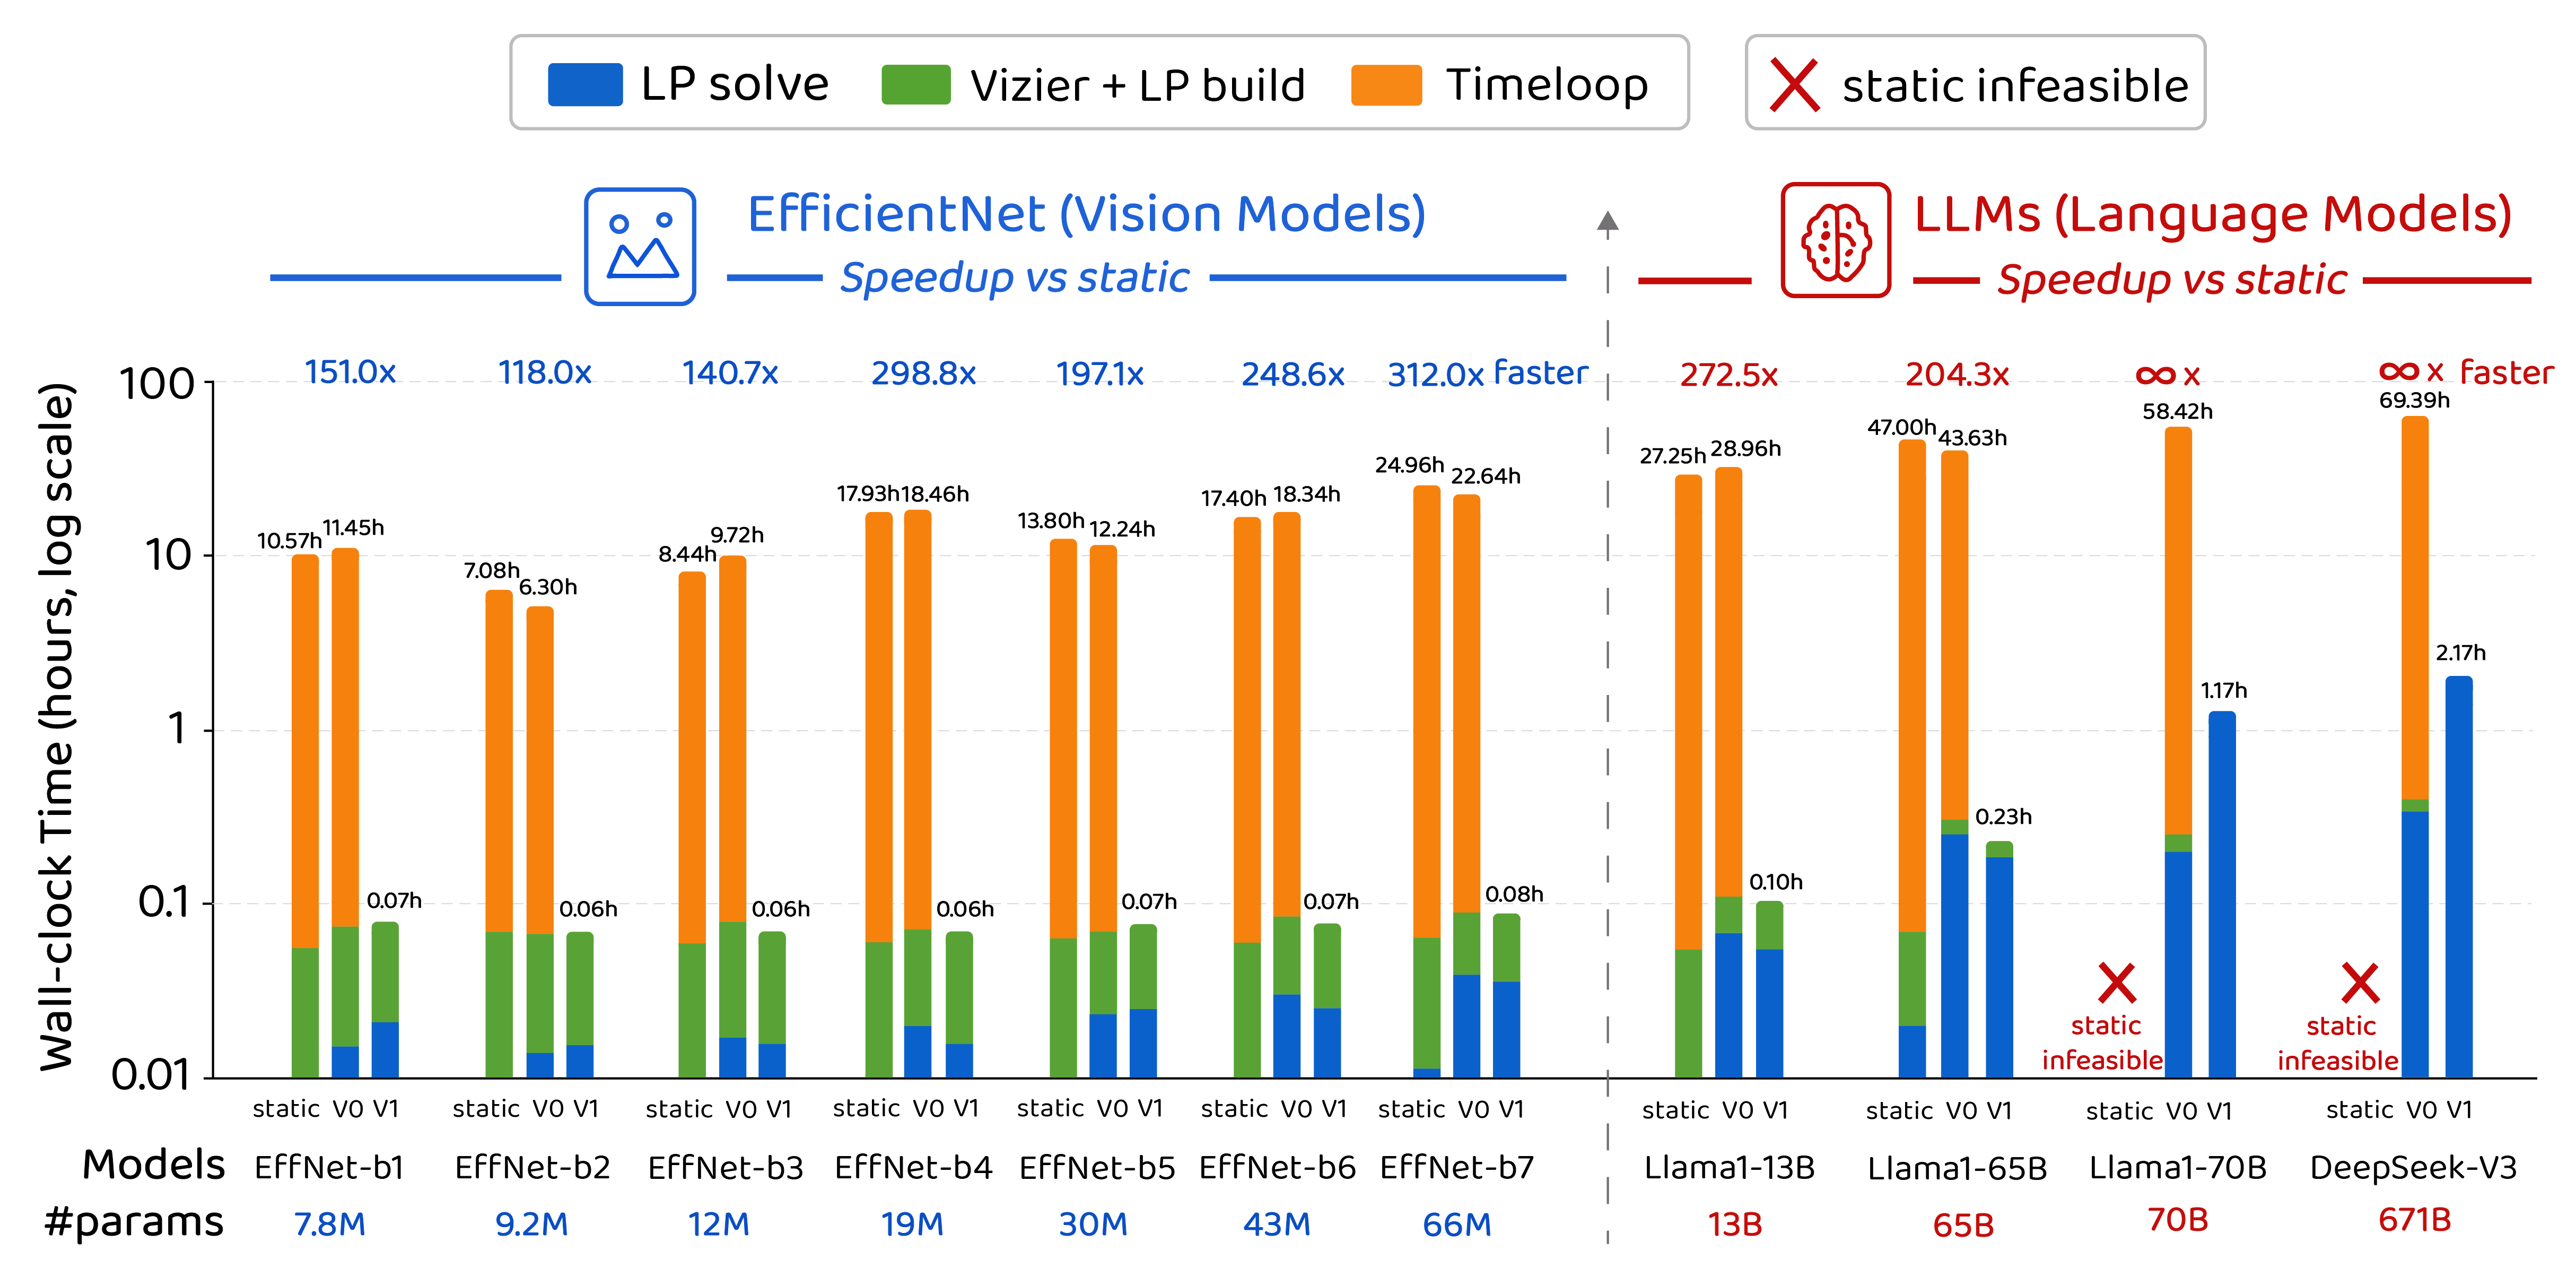
\includegraphics[width=1.0\linewidth]{fig3/wallclock_new_v5.png}
% \caption{Wall-clock time decomposition and performance acceleration across formulations: CHEETAH-V1's internalized tiling eliminates the Timeloop bottleneck, achieving up to 100--300$\times$ faster search than classical static method. Upper bars show wall-clock hours (log scale); annotations show speedup vs.\ static.}
% \label{fig:wallclock}
% \end{figure}

% \subsection{Wall-Clock Acceleration}

% Figure~\ref{fig:wallclock} reveals a striking practical advantage of V1: by internalizing tiling into the LP, it removes Timeloop from the per-trial critical path, collapsing each trial to a single Vizier-proposal and LP-solve step. On EfficientNet models, V1 completes 50 trials 151--312$\times$ faster than the static pipeline. On LLMs the acceleration is even more dramatic: V0 requires 58.42 hours on Llama-70B and 69.39 hours on DeepSeek-V3 for 50 trials, whereas V1 requires only 1.17 hours and 2.17 hours respectively---a ${\sim}93\%$ average reduction. This speedup arises because Timeloop accounts for over 99\% of per-trial latency in the sequential pipeline (Figure~\ref{fig:timeloop-time}), and V1 eliminates this bottleneck entirely via precomputed Pareto tiling sets that are reused across all Vizier trials sharing the same compute configuration class. The combination of higher speedup \emph{and} dramatically lower search cost makes V1 strictly dominant: it explores a larger feasible design space in a fraction of the wall-clock time.

% % This demonstrates that by exploiting structural invariance and GPU-accelerated mathematical optimization, CHEETAH-V1 reduces the end-to-end co-design search time from days to under 2.2 hours—a ${\sim}93\%$ average reduction—while discovering architectural points that deliver up to $35\times$ speedup over the TPU-v3 baseline.

% % Figure~\ref{fig:pareto} shows the Pareto frontier of best-achieved Perf/TDP versus wall-clock search cost. V1 strictly dominates both V0 and static at every time budget: within 10 minutes of search, V1 already exceeds the best Perf/TDP that V0 or static achieve after 60+ minutes. The V1 Pareto frontier reaches ${\sim}35\times$ Perf/TDP, roughly $3\times$ higher than the V0/static frontier at ${\sim}10\text{--}12\times$. This gap reflects two compounding advantages: V1 explores a strictly larger feasible region (joint tiling-fusion), and it eliminates Timeloop from the per-trial critical path, allowing more trials within any fixed time budget.



% \paragraph{LLM Architect vs.\ Optimizer.} Modelled on SkyDiscovery~\citep{skydiscover2026}, the LLM Architect prunes
% the outer search loop by proposing campaign patches rather than
% predicting raw performance. It analyses a Causal Ledger containing
% invalid rates, MFU, and solver diagnostics to suggest constrained
% hardware neighbourhoods for Vizier to explore locally. The V1 LP
% remains the ground-truth evaluator, supported by a Roofline Auditor
% that rejects physically impossible results.
% In a widened search space, the LLM loop reduces invalid evaluations
% from $24.5\%$ to $5.9\%$ on average --- a $4.1\times$ reduction in wasted
% trials --- while reaching the same optimal Perf/TDP scores as full-space
% Vizier. This demonstrates that the LLM's role is steering Bayesian
% optimisation toward feasible, workload-appropriate subspaces rather than
% replacing the solver. We provide exact prompts in Appendix~\ref{app:prompt} for full replication of results, as well as two specific cases studies of real-world use cases.

% % \subsubsection{LLM Architect vs. Optimizer}
% % The LLM Architect framework is modeled on SkyDiscover, and efficiently prunes the large outer hardware search loop by proposing campaign patches. Rather than predicting performance, the Architect reads a compact Causal Ledger containing invalid-rate history, MFU, roofline lower-bound checks, and LP diagnostics, then proposes a constrained hardware neighborhood for Vizier to search locally. The V1 LP remains the sole performance evaluator: for each candidate, it solves the joint tiling, fusion, placement, and rematerialization LP, while a deterministic Roofline Auditor rejects physically impossible results. In the widened V1 search space, all methods reach the same capped V1 Perf/TDP ceiling, so the key differentiator is search efficiency. The LLM loop reduces invalid hardware evaluations from 24.5\% under full-space Vizier to 5.9\% on average across five workloads, a 4.1× reduction in wasted trials, while preserving the same best V1 score. This shows that the LLM’s contribution is not replacing Vizier or the solver, but steering Bayesian optimization toward feasible, workload-appropriate architectural neighborhoods with far less wasted trials. This also sets the foundation for future work, where the LLM in the loop can adhere to follow more complex human reasoning signals.
% \begin{figure}[ht!]
%     \centering
% 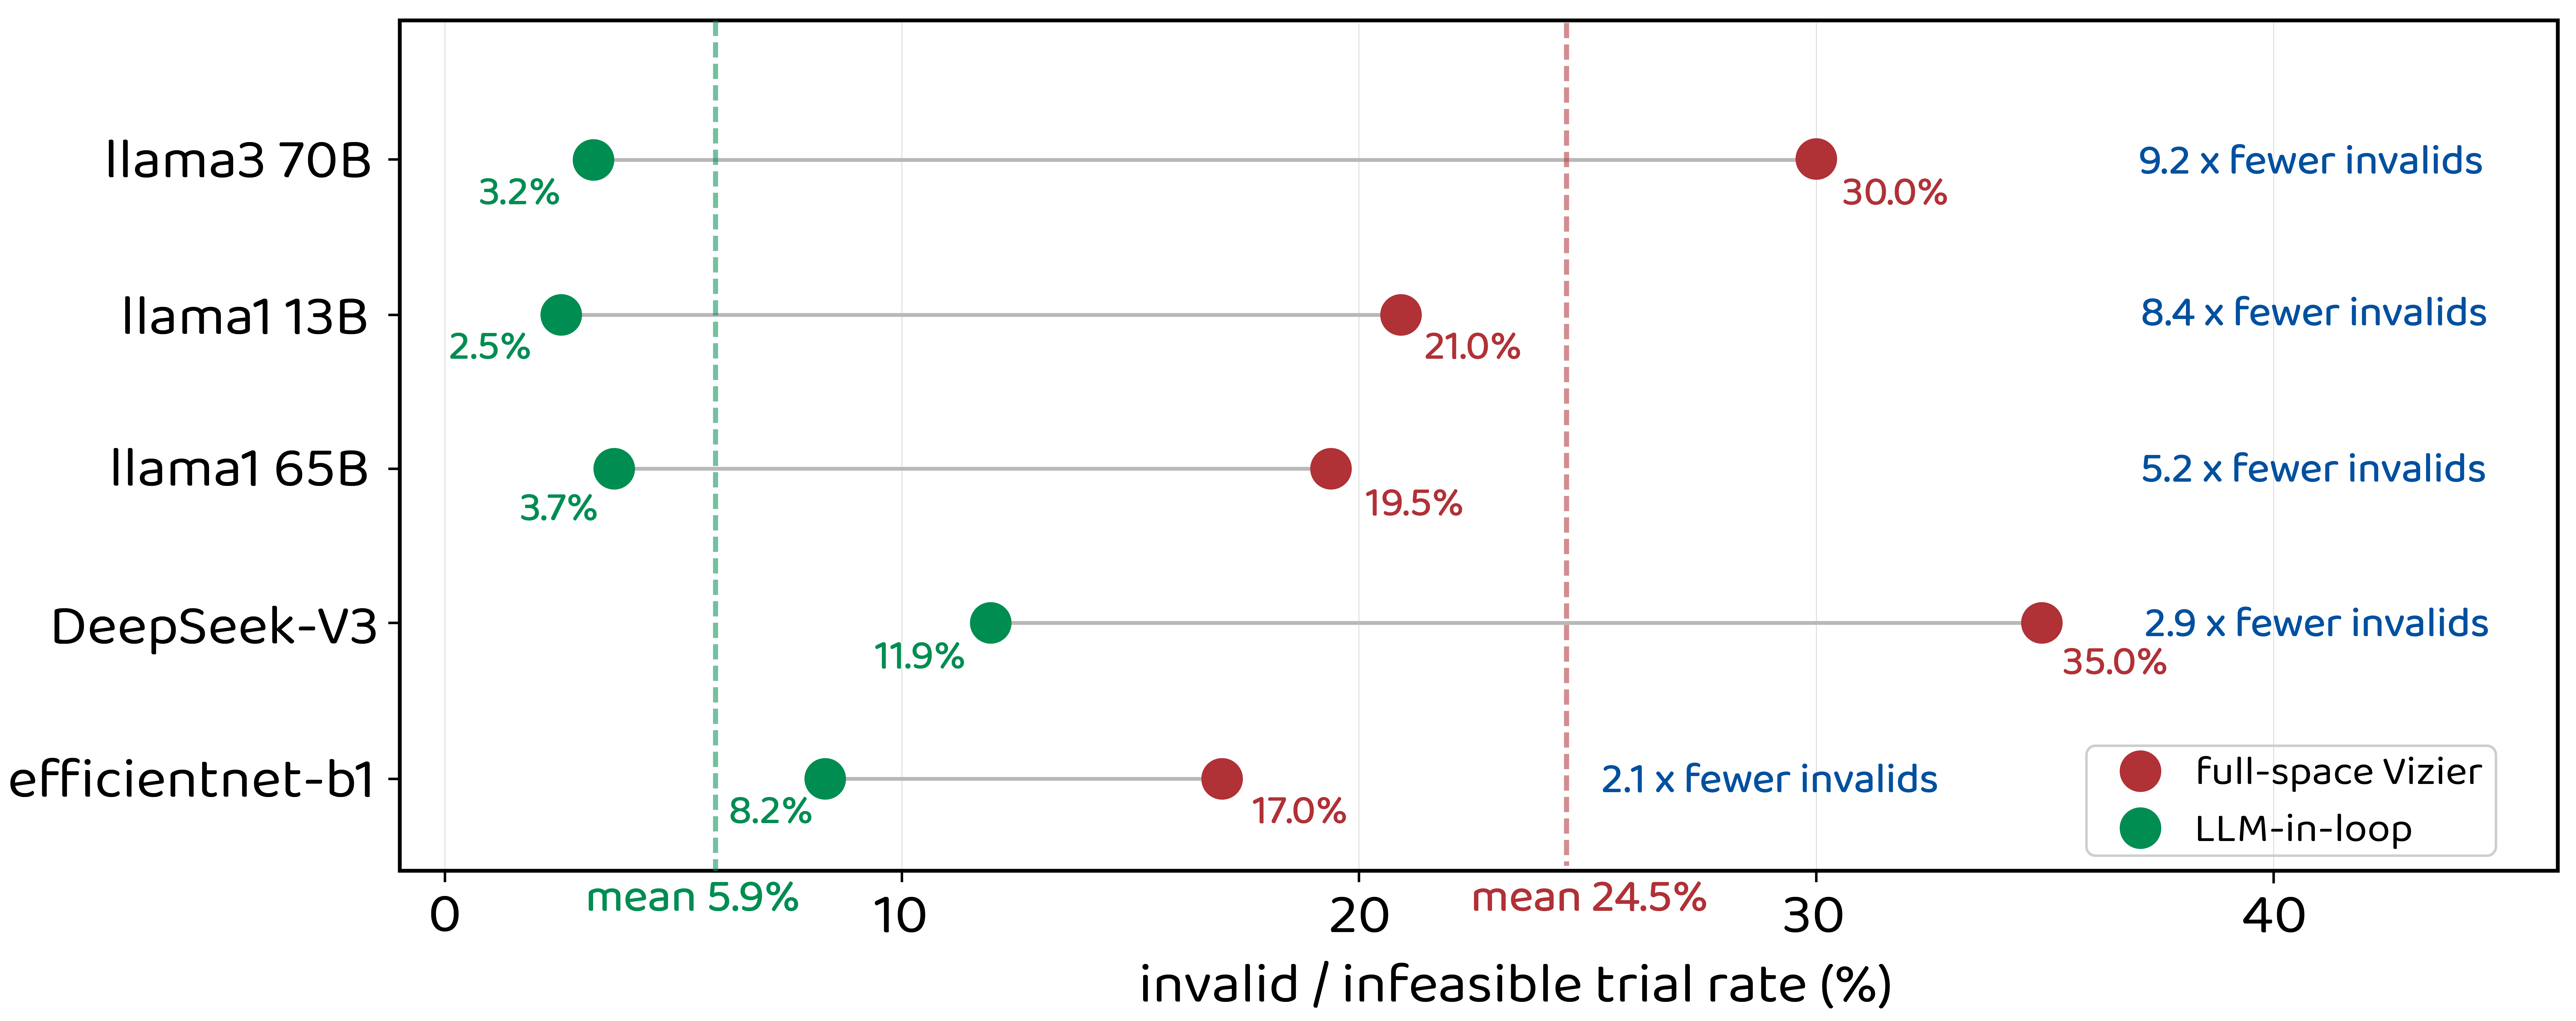
\includegraphics[width=0.85\linewidth]{fig3/llm_guide_v1.png}
% \caption{Invalid/infeasible trial rate (\%) for full-space Vizier vs.\ LLM-in-loop across five workloads. The LLM Architect reduces the mean invalid rate from 24.5\% to 5.9\% (4.1×$\times$
% × reduction), with the largest gains on LLM workloads where the hardware search space is most prone to infeasible configurations.}\label{fig:llm}
% \end{figure}



% % The LLM should not just ask, “What chip has the best Perf/TDP?” We aim to answer the question “Given this user’s workload and deployment goal, what is the architectural region to search for this deployment task?”. Therefore we have the LLM emit profile-conditioned campaigns that take specific user inference tasks into consideration. For each $(\text{deployment profile},\ \text{workload})$ cell, we ran a
% % 200-trial LLM-Architect experiment using the same Qwen2.5-7B-Instruct + LoRA with differing user input profiles. At the start of each round, the prompt was assembled from a fixed system
% % prompt, the active deployment profile, three few-shot examples, and a per-round user message containing the workload, recent feedback signals, current search bounds, and the causal ledger.
% % The Strategist returned a one-line JSON campaign patch, which the
% % validator accepted only if it was a strict legal subset of the parent space, satisfied hard rules such as patch-volume $\leq 10\%$, ridgepoint and MAC/BW constraints, and avoided forbidden regions.

% % Thus, the experiment isolates whether the profile-conditioned LLM prompt alone can steer the same V1 evaluator toward different hardware families under different deployment intents.



% % \todo{Compare convergence rate of LLM-guided hardware search vs.\ Vizier-only (Bayesian, LCS, random baselines) in the style of FAST Figure~11. Report:
% % \begin{itemize}
% %     \item Number of trials to reach $X\%$ of best Perf/TDP found by 5,000-trial Vizier
% %     \item Quality of LLM-proposed configurations vs.\ Vizier-proposed configurations
% %     \item Qualitative analysis of LLM reasoning about hardware bottlenecks
% % \end{itemize}
% % }

% % \subsubsection{ROI Analysis}

% % \todo{Update FAST's ROI analysis (Table~4) with the improved Perf/TDP numbers from FAST-CORGI. Report deployment volumes required to reach 1$\times$, 2$\times$, 4$\times$ ROI targets. If Perf/TDP improvements are larger than FAST's, the break-even deployment volume should decrease correspondingly.}

% % \subsubsection{Pareto Frontier}

% % \todo{Plot the Perf/TDP vs.\ area Pareto frontier for V1-optimized designs compared to FAST and TPU-v3 baseline, analogous to FAST Figure~12.}


% page limit edit

% % \section{Experiments}
% % \label{sec:experiments}
% % In all cases we use an adapted JAX PDLP solver for large models at LLama70-B and DeepSeekv3 scale across all three methods (Static, CHEETAH-V0, CHEETAH-V1); and use HiGHS as the default solver for all other smaller neural network models. In order to be consistent with prior work, our experimental results are presented as orders of speedup / performance against a vanilla TPU-V3. This is also since TPUs are targeted for NN accelerators (as opposed to GPUs), and the TPU-V3 has the most information publically released, making it possible for us to simluate it more accurately. 

% % \subsection{Experimental Setup}

% % \paragraph{Static Sequential Baseline.}
% % We compare against the static optimization FAST framework using a simulated TPU-v3 baseline normalized to a sub-10nm process technology, following the same methodology as Zhang \etal. The baseline simulator is well-correlated with production hardware: on average within 8.2\,$\pm$\,2.7\% of profiled TPU-v3 performance. We evaluate against a \emph{simulated} TPU-v3 baseline to account for optimistic simulator assumptions.

% % We evaluate across 11 representative workloads: EfficientNet-B1 through EfficientNet-B7, Llama13, 65, 70 models, and DeepSeek-V3-MoE. These workloads stress different parts of the hardware design space: EfficientNet stresses low-operational-intensity depthwise convolutions, while Llama and DeepSeek stress memory capacity, bandwidth, and large matrix operations. 

% % \textbf{Single-workload specialization.} Each neural network workload is optimized independently. This experiment measures the best workload-specific hardware found under a fixed trial budget and identifies architectural preferences such as Global Memory size, bandwidth, MAC count, and systolic shape. In the case of Staitic and V0 methods, the pipeline involves: Vizier - Timeloop - LP solver. In the case of the V1 method, the pipeline is simplified to Vizier - LP solver. In each case we iterate for 100 trials per method x NN. 

% % % \textbf{Fixed-hardware-workload generalization.} We search for general-purpose datapaths that perform well across the workload suite. The objective is a harmonic or geometric aggregation of per-workload Perf/TDP, forcing the search to balance CNN-style memory pressure and LLM-style compute/memory trade-offs.

% % \textbf{LLM-Architect guides outer search.} We the LLM-guided outer-loop controller which proposes search-space interventions for Vizier. The advantage of the CHEETAH-V1 formulation is it removes dependence of Timeloop in the loop. Therefore the loop is reduced to just Vizier-LP solve, which dramatically speeds up the iterative process, thus permitting the LLM-Architect outer loop. The LLM is only permitted to change the search neighborhood of Vizier's input, the strict LP formulation on the inner loop does not change. This ensures mathematical and physical constraints are upheld in the space of co-design. 

% % % \paragraph{Optimization framework.}
% % % For the outer hardware search loop, we use Google Vizier with LCS optimization and safe search, running 100 trials per experiment (method X NN x Exp). Each trial invokes the LP solver for the inner optimization. The Static and V0 methods additionally have Timeloop in the loop (Vizier-Timeloop-LP solve). The advantage of the v1 formulation is it removes dependance of Timeloop in the loop. Therefore the loop is reduced to just Vizier-Lp solve, which dramatically speeds up the iterative process, thus permitted the Strategic LLM outer loop.

% % We validate our framework through a multi-level audit process to ensure physical and numerical rigor.
% % \textbf{Roofline Auditor.}
% % A deterministic Roofline Auditor enforces physical feasibility by
% % verifying that LP-predicted latencies never fall below the theoretical
% % bound
% % \begin{equation}
% %     \mathrm{LB} = \max\!\left(t_{\mathrm{compute}},\;
% %     t_{\mathrm{memory}}\right),
% %     \label{eq:roofline_lb_val}
% % \end{equation}
% % where $t_{\mathrm{compute}}$ and $t_{\mathrm{memory}}$ represent the
% % peak compute and memory bandwidth floors, respectively.
% % All reported V0/V1 results are roofline-feasible with valid
% % $\mathrm{MFU}_{\mathrm{bound}}$ and memory utilization metrics.

% % \textbf{Campaign Validator.}
% % A deterministic Campaign Validator legalizes LLM-proposed architectural
% % neighbourhoods by enforcing hard hardware constraints — including TDP
% % caps, area limits, and power-of-two parameter ranges — prior to Vizier
% % sampling.

% % \textbf{Causal Ledger.}
% % A Causal Ledger tracks LLM interventions and observed outcomes,
% % preventing redundant exploration of empirically invalid regions and
% % ensuring full auditability of the search loop.

% % \textbf{Solver Diagnostics.}
% % We monitor solver diagnostics including primal/dual residuals, duality
% % gap, and rounding gap. Designs are treated as trustworthy only when both
% % the continuous LP relaxation and the rounded integer solution are
% % numerically well-behaved.


% % \subsection{Main Results}

% % % \subsubsection{V0 vs.\ FAST Static Fusion}

% % % \todo{Insert results table and figure comparing V0 (time-indexed placement + rematerialization) against FAST's static fusion ILP on all benchmarks. Key metrics: Perf/TDP improvement, fusion efficiency (\% of DRAM stall time eliminated), rematerialization frequency (how often does the solver choose to recompute rather than reload?).}

% % % \paragraph{Expected findings.}
% % % V0's dynamic placement should show the largest gains on workloads with: (1)~tight Global Memory budgets where static pinning wastes capacity on tensors that are only needed briefly, (2)~long dependency chains where tensor lifetimes vary substantially, and (3)~cheap-to-recompute operations with large activations (\eg, depthwise convolutions in EfficientNet).

% % % \subsubsection{V1 vs.\ V0: Joint Tiling and Fusion}

% % % \todo{Insert results table and figure comparing V1 against V0 on all benchmarks. Key metrics: Perf/TDP improvement, number of operations where V1 selects a different tiling configuration than Timeloop's greedy choice, and the resulting compute efficiency vs.\ fusion trade-off.}

% % % \paragraph{Expected findings.}
% % % V1 should show the largest gains on architectures with highly diverse layer types where a single tiling configuration cannot serve all operations well. EfficientNet (depthwise + pointwise convolutions with 100$\times$ variation in working-set sizes) and hybrid CNN-transformer models (convolutions + attention + MLP with fundamentally different compute-memory profiles) are expected to benefit most.


% % % \subsubsection{stiatic vs v0 vs v1}
% % % \begin{figure}[ht!]
% % %     \centering
% % %     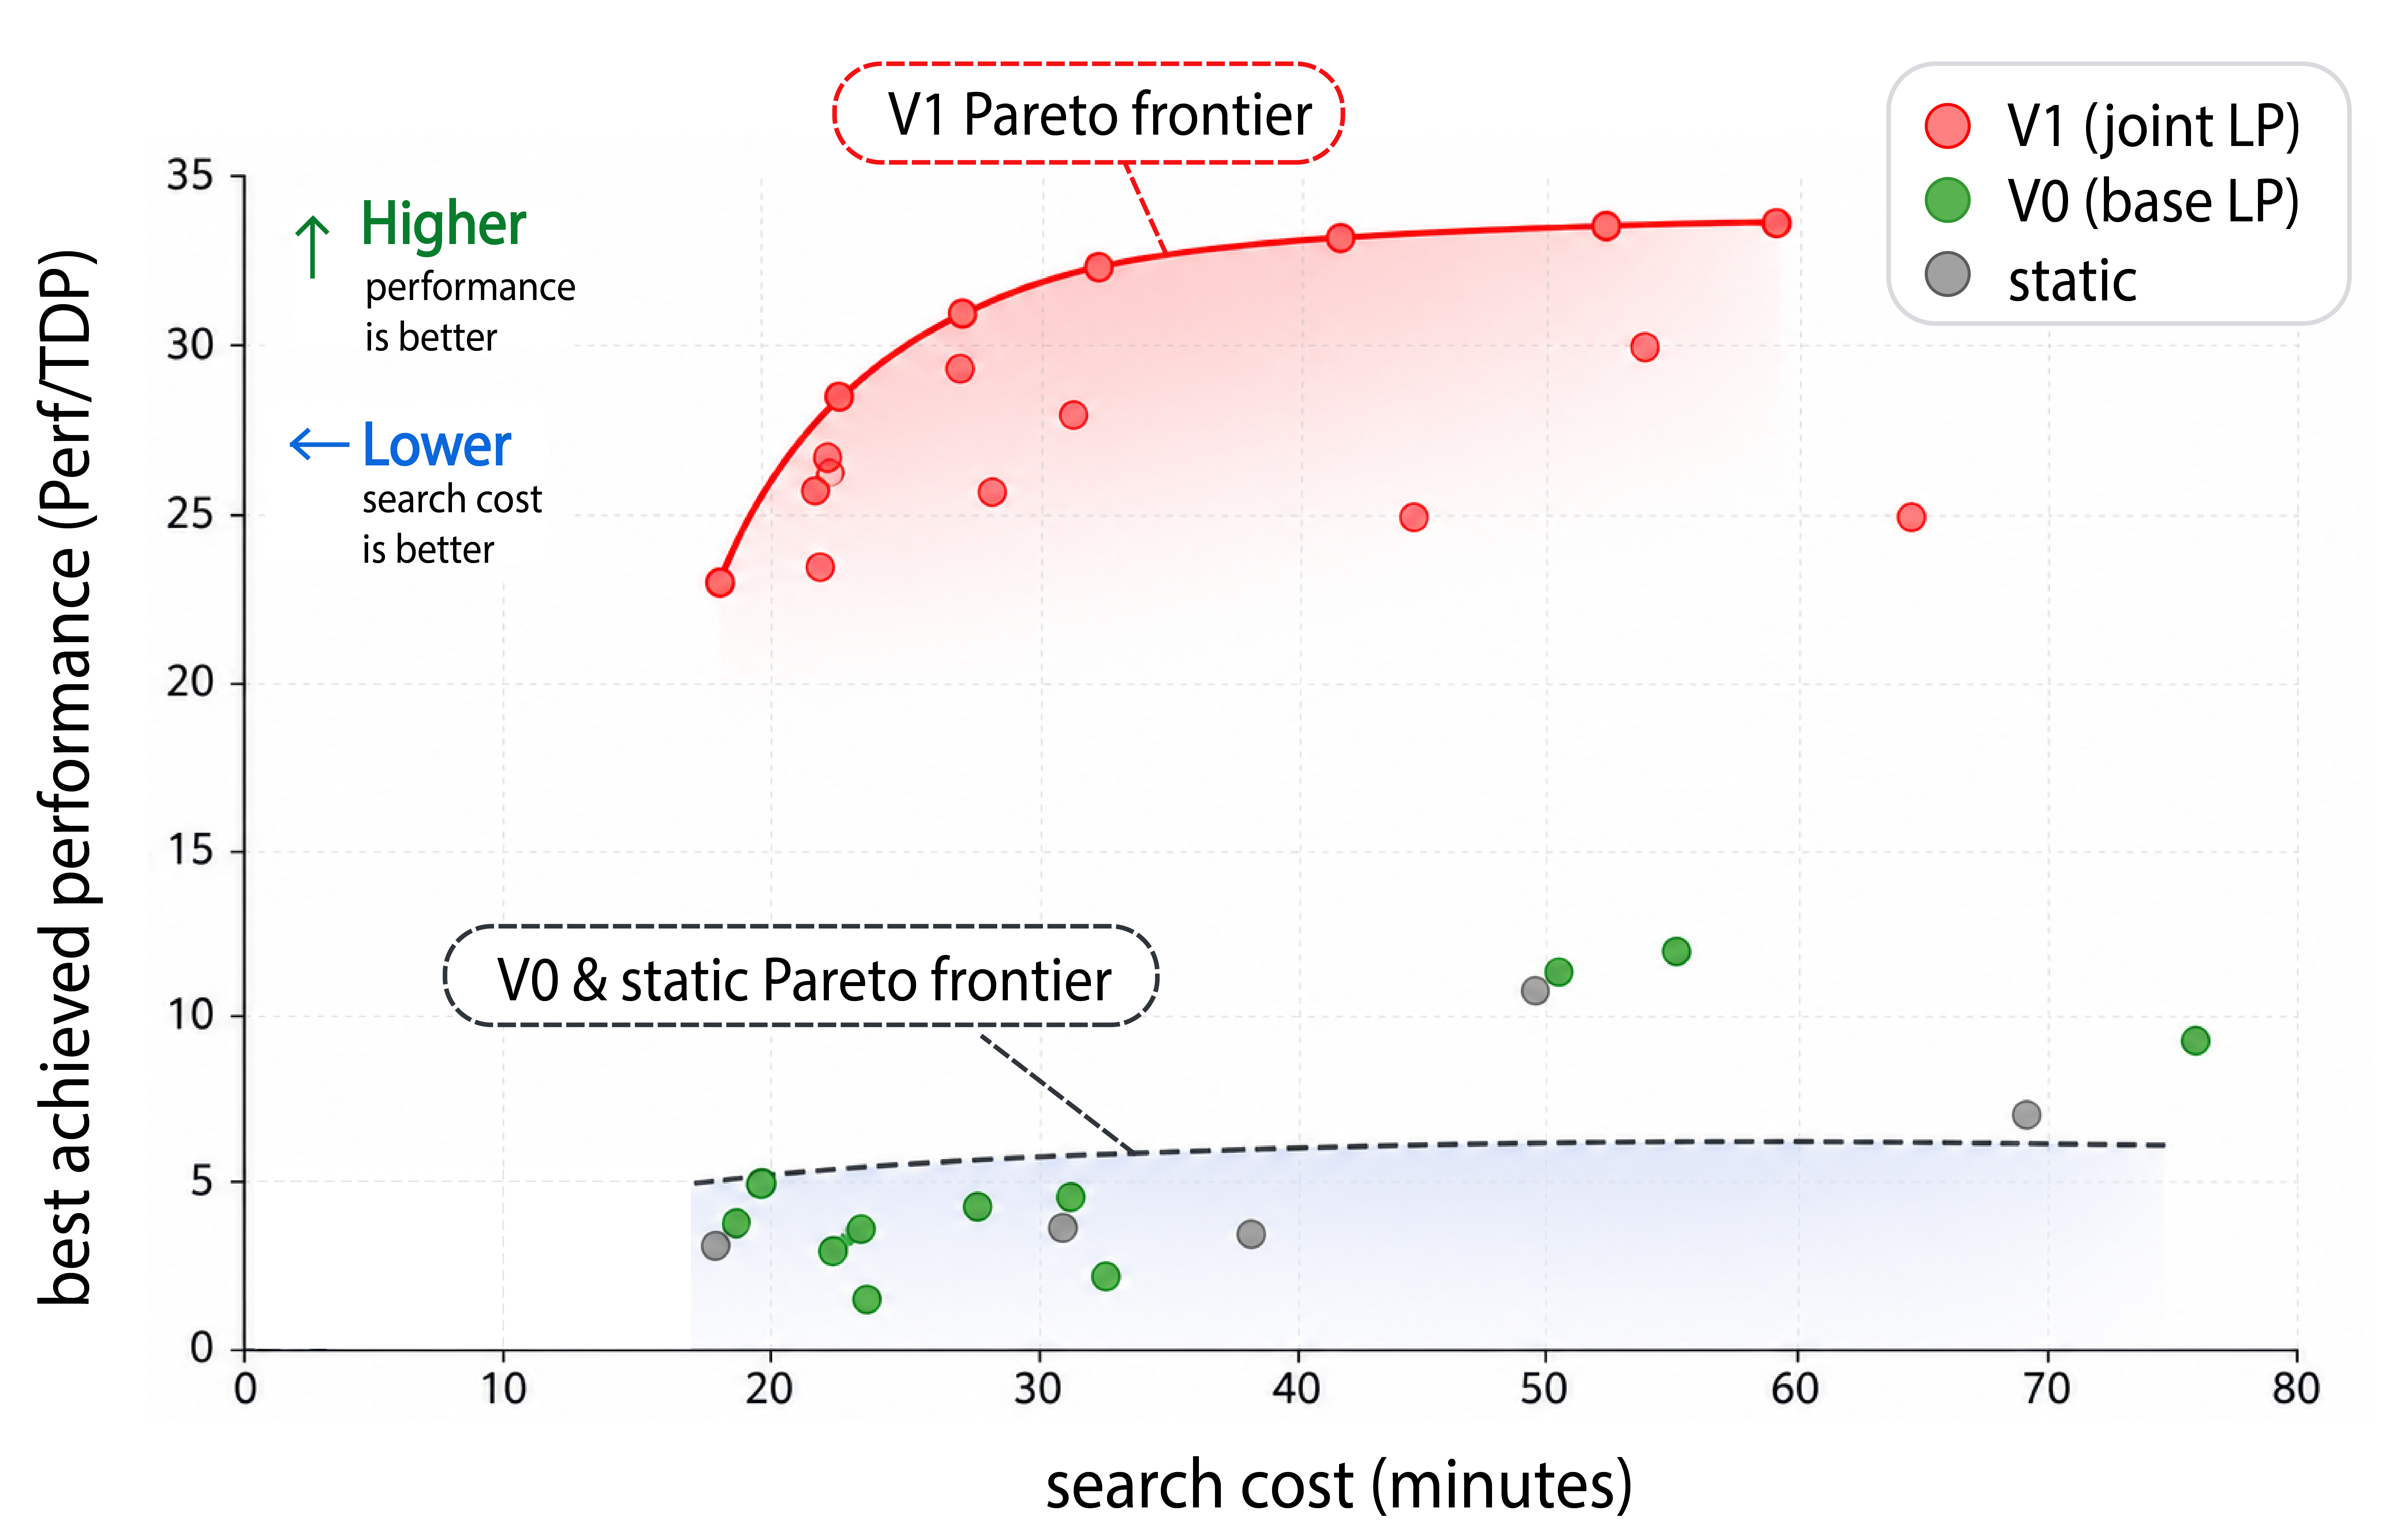
\includegraphics[width=0.7\linewidth]{figs/pareto_v2.png}
% % %     \caption{pareto frontier plot}
% % % \end{figure}
% % \begin{figure}[ht!]
% %     \centering
% % 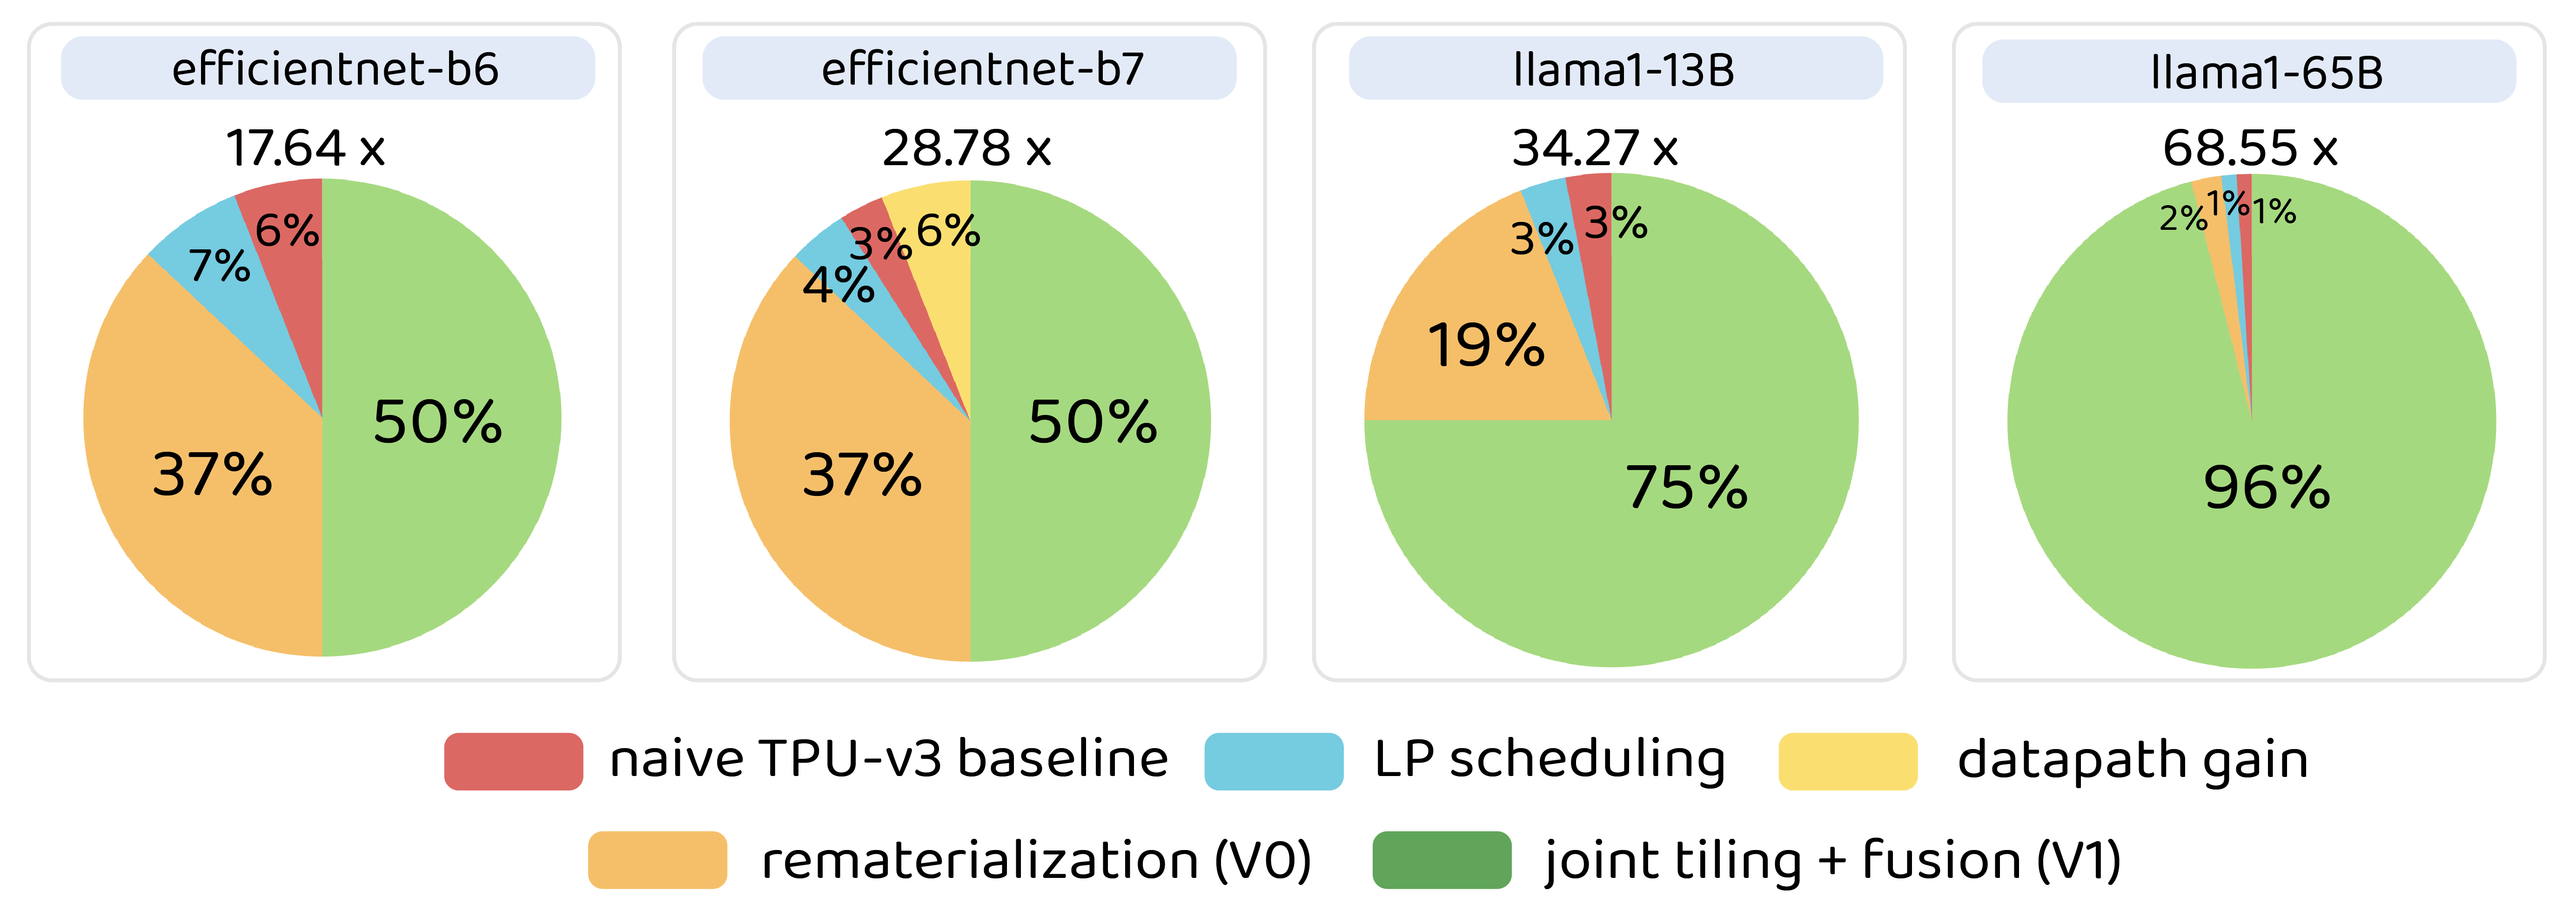
\includegraphics[width=0.85\linewidth]{fig3/speedup_decomposition_final_v2.png}
% % \caption{Speedup decomposition over naive TPU-v3 baseline. Each pie shows the 
% % relative contribution of four optimization sources to the total speedup. CHEETAH-V1 joint tiling + fusion dominates on all workloads, 
% % especially on larger models where memory management is the primary bottleneck.}\label{fig:accel_decompose}
% % \end{figure}
% % \subsubsection{Static Baseline vs.\ CHEETAH-V0 vs.\ CHEETAH-V1 Unlock Progressive Gains}


% % Figure~\ref{fig:accel_decompose} decomposes the total speedup over a naive TPU-v3 baseline into four sources: LP-based scheduling and fusion, datapath gain from hardware search, dynamic rematerialization (CHEETAH-V0), and joint tiling + fusion (CHEETAH-V1).

% % The dominant contributor across all workloads is V1's joint tiling-fusion 
% % optimization. On EfficientNet-B1, V1 accounts for 50\% of total speedup, 
% % with LP scheduling (28\%) and datapath gain (22\%) splitting the remainder---and 
% % no rematerialization benefit, consistent with B1's small activation footprint 
% % fitting comfortably in Global Memory. B3--B4 show a similar 50\% V1 share, but 
% % V0 rematerialization now contributes 25\%, reflecting the growing value of 
% % recomputing large depthwise activations rather than reloading them from DRAM. 
% % From B5 onward, V1's share rises sharply to 75--88\%, as the increasing 
% % model size makes joint tiling-fusion the primary lever: memory management 
% % dominates, and the remaining sources (LP scheduling, V0, datapath) each shrink 
% % to single-digit percentages. The same pattern holds on Llama, where V1 accounts 
% % for 83--87\% of the total speedup.

% % % \begin{wrapfigure}{r}{0.48\textwidth}
% % %     \centering
% % %     \vspace{-12pt}
% % %     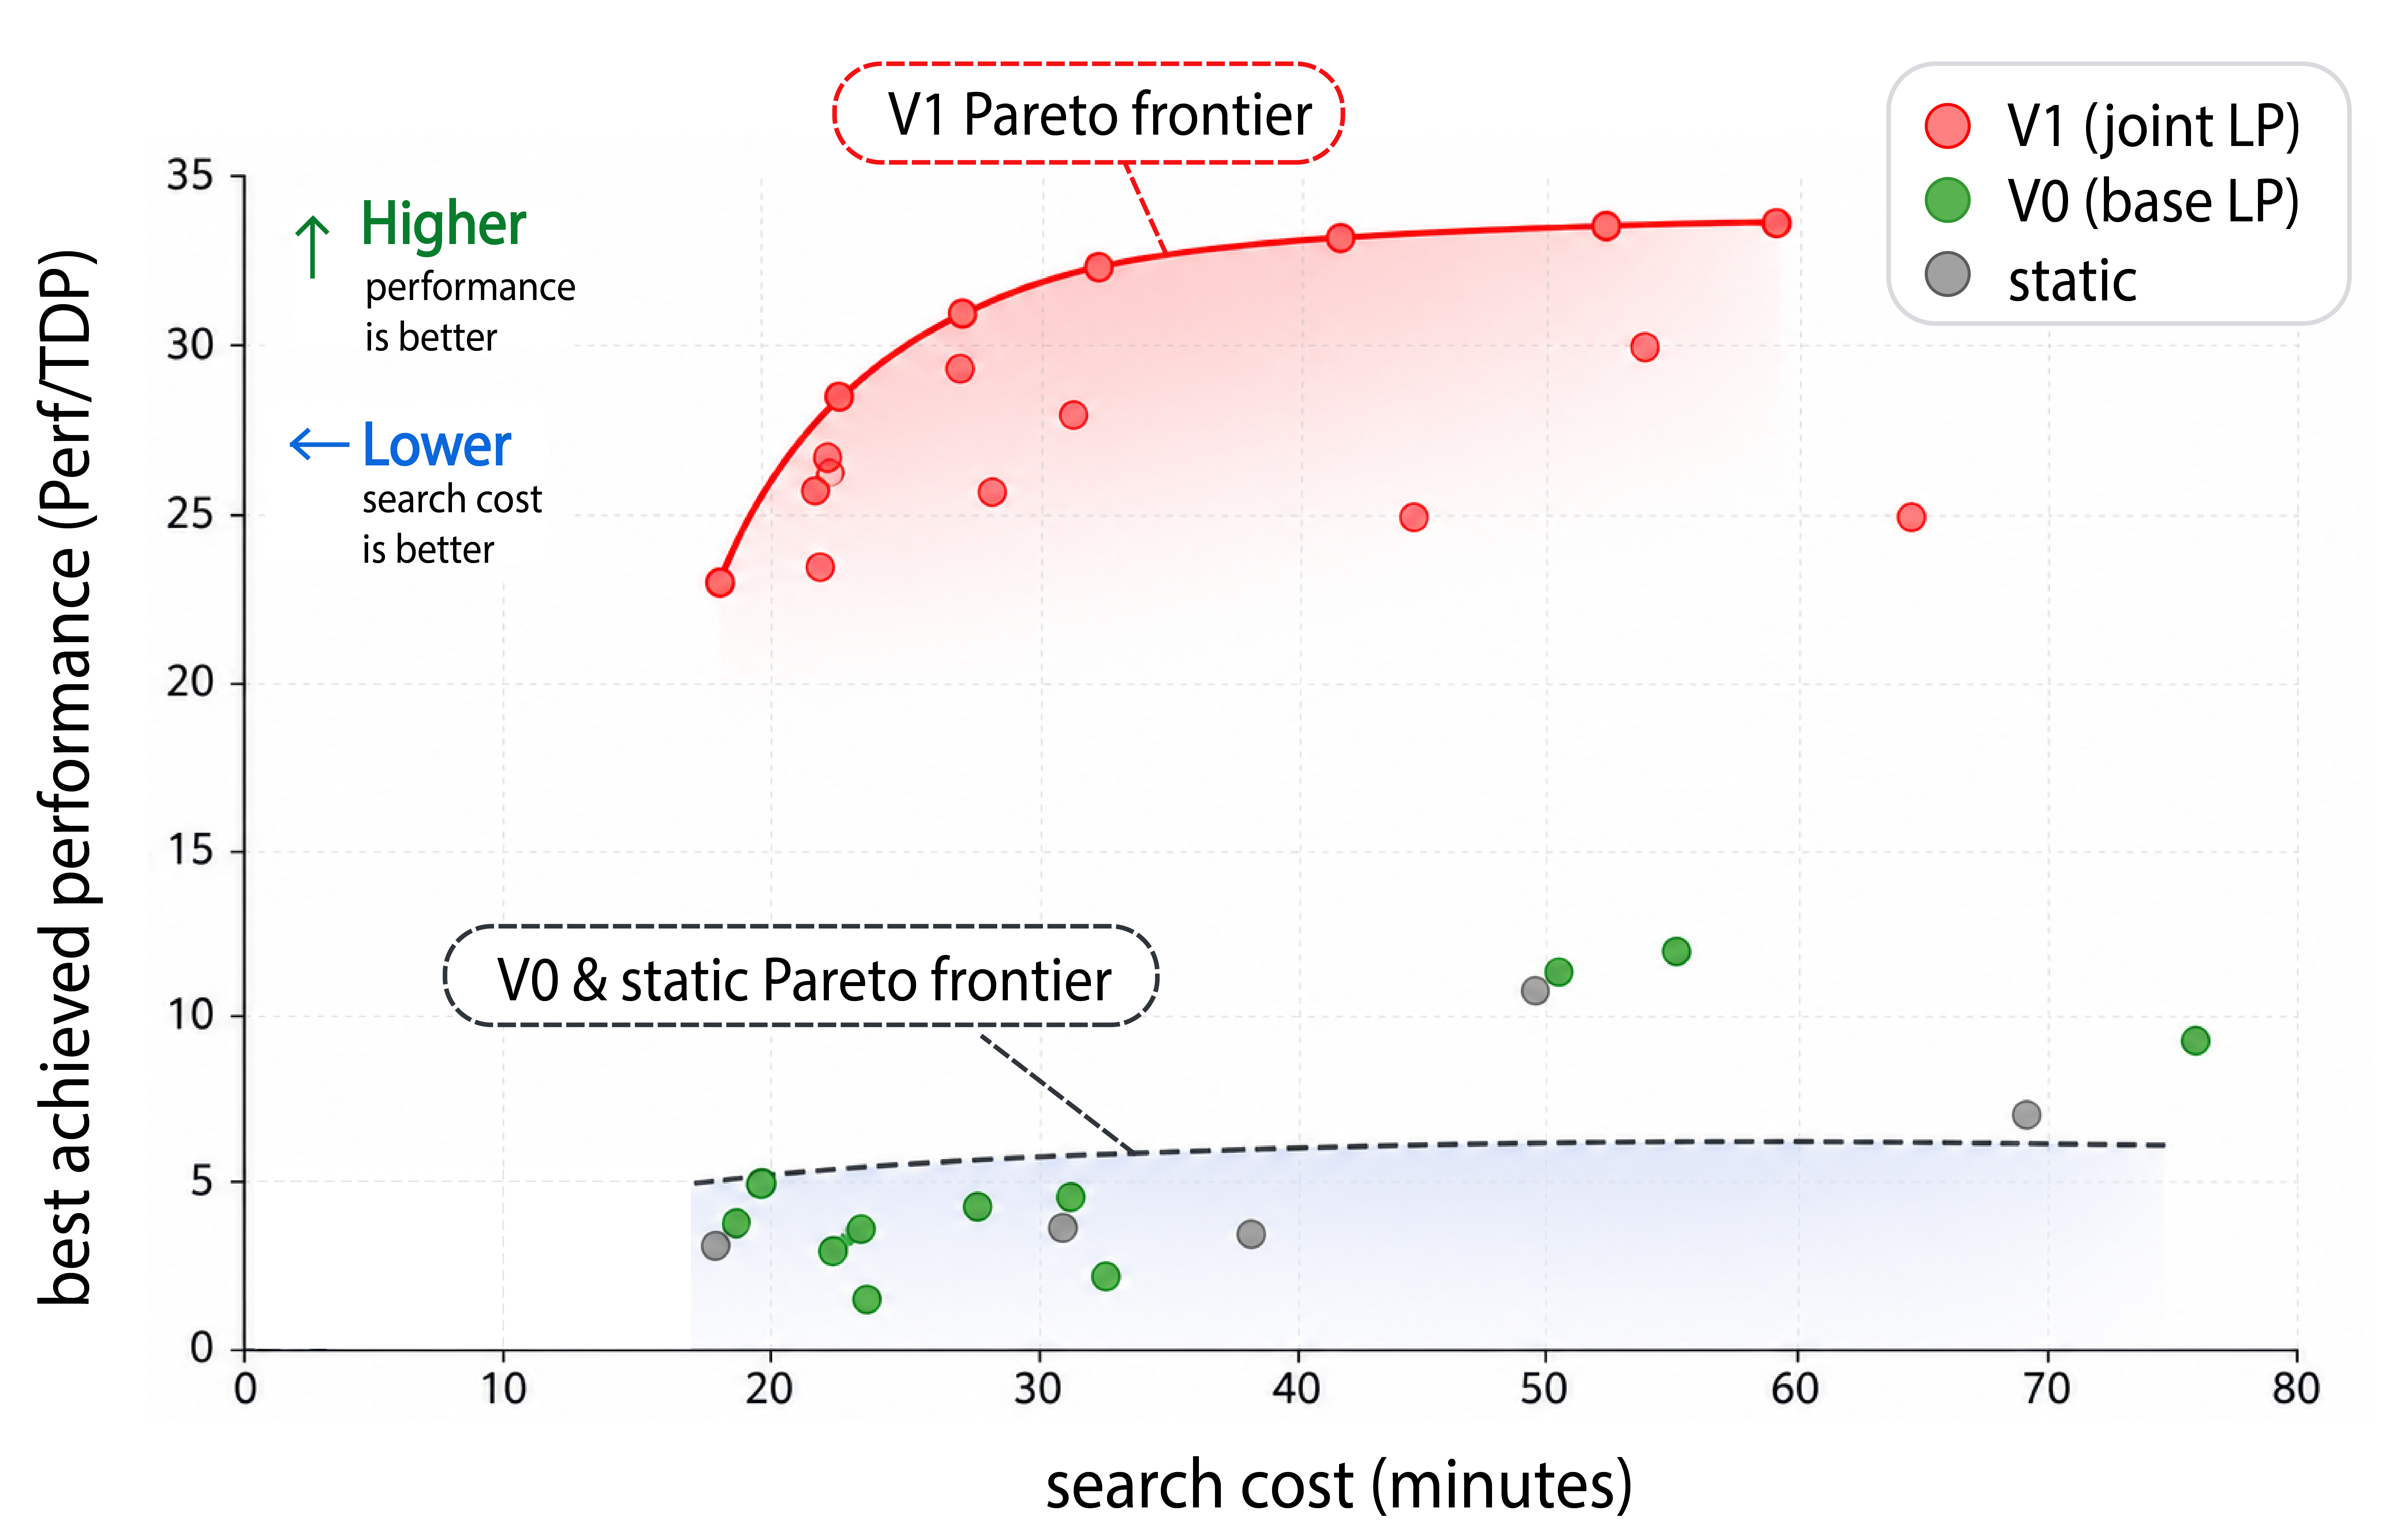
\includegraphics[width=0.48\textwidth]{figs/pareto_v2.png}
% % %     \vspace{-18pt}
% % %     \caption{Search cost vs.\ Perf/TDP Pareto frontier. V1 dominates V0 and static across all time budgets.}
% % %     \label{fig:pareto}
% % %     \vspace{-10pt}
% % % \end{wrapfigure}

% % Critically, Figure~\ref{fig:speedup} shows static fusion method is \emph{infeasible} on modern large models (Llama-70B, and DeepSeek-V3), because their large activation tensors cannot fit under a static pinning policy. The V0 formulation resolves feasibility for on large models via dynamic placement but remains time-intensive for a small number of 50 trials: measuring 58.42 hours on Llama-70B and 69.39 hours on DeepSeek-V3 (Figure~\ref{fig:wallclock}). In contrast Figures~\ref{fig:wallclock} and ~\ref{fig:speedup}, show the CHEETAH-V1 formulation out performs comparitive strategies in terms of speedup against the TPU-V3 baseline, and require only 1.17 hours on Llama-70B and 2.17 hours on DeepSeekv3 for 50 trails---a ${\sim}93\%$ average reduction. The powerful joint formulation is able to select memory-efficient tiling configurations alongside placement, achieving feasibility across the entire workload suite, demonstrating that joint optimization is not merely an incremental improvement but a qualitative capability unlock for large-scale models.

% % % This demonstrates that by exploiting structural invariance and GPU-accelerated mathematical optimization, CHEETAH-V1 reduces the end-to-end co-design search time from days to under 2.2 hours—a ${\sim}93\%$ average reduction—while discovering architectural points that deliver up to $35\times$ speedup over the TPU-v3 baseline.

% % % Figure~\ref{fig:pareto} shows the Pareto frontier of best-achieved Perf/TDP versus wall-clock search cost. V1 strictly dominates both V0 and static at every time budget: within 10 minutes of search, V1 already exceeds the best Perf/TDP that V0 or static achieve after 60+ minutes. The V1 Pareto frontier reaches ${\sim}35\times$ Perf/TDP, roughly $3\times$ higher than the V0/static frontier at ${\sim}10\text{--}12\times$. This gap reflects two compounding advantages: V1 explores a strictly larger feasible region (joint tiling-fusion), and it eliminates Timeloop from the per-trial critical path, allowing more trials within any fixed time budget.



% % \paragraph{Practical insight.}
% % Both LPs are extreme-aspect-ratio sparse: for \texttt{llama3\_70b},
% % $m, n \sim 10^6$ and $\mathrm{nnz} \sim 5 \times 10^6$, giving roughly
% % 1 nonzero per million matrix entries.
% % The time-band structure means a coordinate-descent or stochastic PDHG
% % solver would converge in $\mathcal{O}(T)$ sweeps if bands were the only
% % structure.
% % The capacity rows in both V0 and V1 LP formulations are the sole feature breaking strict banded structure, and they are precisely what couples the schedule globally. This is the desired behavior of a memory-aware placement formulation.

% % % \todo{Report LP solve times for V0 and V1 across all benchmarks. Compare wall-clock time per trial against FAST's SCIP-based ILP solver (20 min timeout). Report LP relaxation gap: how often do fractional solutions need integer rounding, and what is the quality loss from rounding?}

% % \paragraph{Structural invariance.}
% % For a fixed workload and LP formulation, the LP constraint matrix
% % has an invariant sparsity pattern across trials: the row/column
% % dimensions and nonzero locations are determined only by the model graph structure — layer count $L$, timestep count $T$, edge set $E$, and Pareto count $C$ — not by the hardware candidate.
% % Vizier changes only numerical values such as cycle coefficients,
% % memory-capacity bounds, bandwidth-scaled access costs, objective weights, and TDP/area parameters. 
% % This invariance allows us to reuse the same sparse matrix structure,
% % variable ordering, block layout, and JIT-compiled sparse kernels in our adapted JAX PDLP solver across all hardware trials for a given workload.

% % Numerically, we apply the same diagonal preconditioning pipeline
% % on each trial: a structural presolve with 20 log-geomean Ruiz iterations, followed by the PDLP preprocessing stack with 10 infinity-norm Ruiz iterations and one Pock--Chambolle $\ell_1$-scaling pass. This two-stage diagonal scaling handles the mixed coefficient magnitudes present in V0/V1 matrices — large byte-valued capacity rows together with $\pm 1$ persistence rows — without requiring a fragile matrix factorization.

% % In production, this preconditioning pipeline is reused structurally across trials, recomputes only cheap diagonal scalings, finishes in under one second for matrices with approximately $5 \times 10^6$ nonzeros, and avoids factorization failures entirely because it consists only of $D_1 A D_2$ arithmetic.

% % \subsubsection{LLM Architect vs. Optimizer}
% % The LLM Architect framework is modeled on SkyDiscover, and efficiently prunes the large outer hardware search loop by proposing campaign patches. Rather than predicting performance, the Architect reads a compact Causal Ledger containing invalid-rate history, MFU, roofline lower-bound checks, and LP diagnostics, then proposes a constrained hardware neighborhood for Vizier to search locally. The V1 LP remains the sole performance evaluator: for each candidate, it solves the joint tiling, fusion, placement, and rematerialization LP, while a deterministic Roofline Auditor rejects physically impossible results. In the widened V1 search space, all methods reach the same capped V1 Perf/TDP ceiling, so the key differentiator is search efficiency. The LLM loop reduces invalid hardware evaluations from 24.5\% under full-space Vizier to 5.9\% on average across five workloads, a 4.1× reduction in wasted trials, while preserving the same best V1 score. This shows that the LLM’s contribution is not replacing Vizier or the solver, but steering Bayesian optimization toward feasible, workload-appropriate architectural neighborhoods with far less wasted trials. This also sets the foundation for future work, where the LLM in the loop can adhere to follow more complex human reasoning signals.
% % \begin{figure}[ht!]
% %     \centering
% % 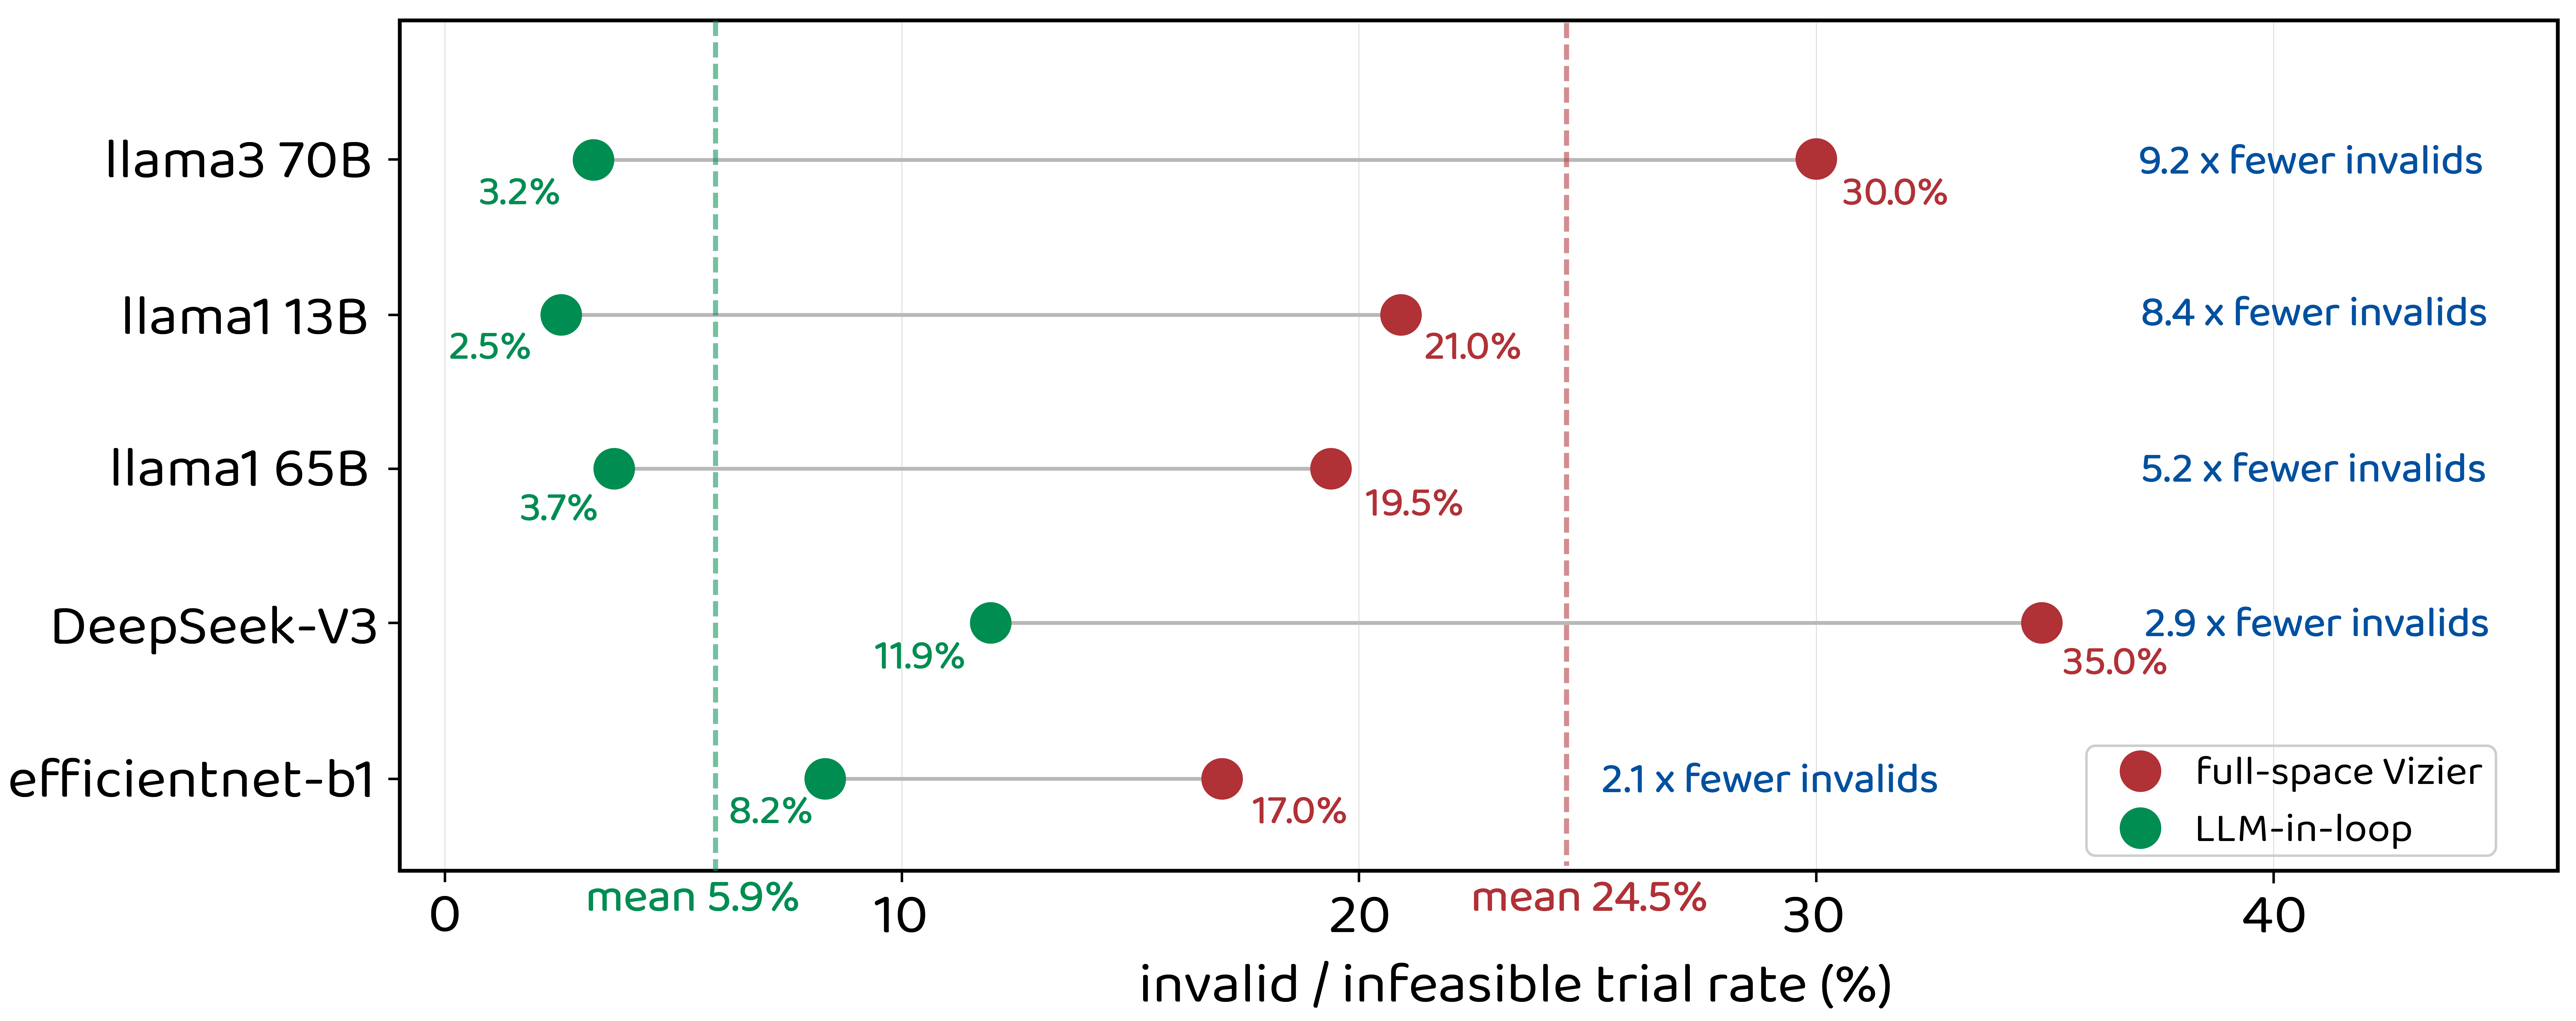
\includegraphics[width=0.85\linewidth]{fig3/llm_guide_v1.png}
% % \caption{Strategic Intelligence vs. Stochastic Brute Force}\label{fig:llm}
% % \end{figure}



% % % The LLM should not just ask, “What chip has the best Perf/TDP?” We aim to answer the question “Given this user’s workload and deployment goal, what is the architectural region to search for this deployment task?”. Therefore we have the LLM emit profile-conditioned campaigns that take specific user inference tasks into consideration. For each $(\text{deployment profile},\ \text{workload})$ cell, we ran a
% % % 200-trial LLM-Architect experiment using the same Qwen2.5-7B-Instruct + LoRA with differing user input profiles. At the start of each round, the prompt was assembled from a fixed system
% % % prompt, the active deployment profile, three few-shot examples, and a per-round user message containing the workload, recent feedback signals, current search bounds, and the causal ledger.
% % % The Strategist returned a one-line JSON campaign patch, which the
% % % validator accepted only if it was a strict legal subset of the parent space, satisfied hard rules such as patch-volume $\leq 10\%$, ridgepoint and MAC/BW constraints, and avoided forbidden regions.

% % % Thus, the experiment isolates whether the profile-conditioned LLM prompt alone can steer the same V1 evaluator toward different hardware families under different deployment intents.



% % % \todo{Compare convergence rate of LLM-guided hardware search vs.\ Vizier-only (Bayesian, LCS, random baselines) in the style of FAST Figure~11. Report:
% % % \begin{itemize}
% % %     \item Number of trials to reach $X\%$ of best Perf/TDP found by 5,000-trial Vizier
% % %     \item Quality of LLM-proposed configurations vs.\ Vizier-proposed configurations
% % %     \item Qualitative analysis of LLM reasoning about hardware bottlenecks
% % % \end{itemize}
% % % }

% % % \subsubsection{ROI Analysis}

% % % \todo{Update FAST's ROI analysis (Table~4) with the improved Perf/TDP numbers from FAST-CORGI. Report deployment volumes required to reach 1$\times$, 2$\times$, 4$\times$ ROI targets. If Perf/TDP improvements are larger than FAST's, the break-even deployment volume should decrease correspondingly.}

% % % \subsubsection{Pareto Frontier}

% % % \todo{Plot the Perf/TDP vs.\ area Pareto frontier for V1-optimized designs compared to FAST and TPU-v3 baseline, analogous to FAST Figure~12.}


% % edit for page limit

% \section{Experiments}
% \label{sec:experiments}
% We implement an adapted JAX PDLP solver for large-scale models (Llama-70B and DeepSeek-V3) across all formulations (Static, V0, V1), while employing HiGHS for smaller networks. To maintain consistency with prior research, results are reported as speedup relative to a simulated TPU-v3 baseline. The TPU-v3 is selected as a benchmark because its architecture is purpose-built for neural network acceleration and its publicly available specifications permit high-fidelity simulation.

% \subsection{Experimental Setup}

% \paragraph{Static Sequential Baseline.}
% We compare against the static optimization FAST framework using a simulated TPU-v3 baseline normalized to a sub-10nm process technology, following the same methodology as Zhang \etal. The baseline simulator is well-correlated with production hardware: on average within 8.2\,$\pm$\,2.7\% of profiled TPU-v3 performance. We evaluate against a \emph{simulated} TPU-v3 baseline to account for optimistic simulator assumptions. We evaluate across 11 representative workloads: EfficientNet-B1 through EfficientNet-B7, Llama13, 65, 70 models, and DeepSeek-V3-MoE. These workloads stress different parts of the hardware design space: EfficientNet stresses low-operational-intensity depthwise convolutions, while Llama and DeepSeek stress memory capacity, bandwidth, and large matrix operations. 

% \textbf{Single-workload specialization.} Each neural network workload is optimized independently. This experiment measures the best workload-specific hardware found under a fixed trial budget and identifies architectural preferences such as Global Memory size, bandwidth, MAC count, and systolic shape. In the case of Staitic and V0 methods, the pipeline involves: Vizier - Timeloop - LP solver. In the case of the V1 method, the pipeline is simplified to Vizier - LP solver. In each case we iterate for 100 trials per method x NN. 

% % \textbf{Fixed-hardware-workload generalization.} We search for general-purpose datapaths that perform well across the workload suite. The objective is a harmonic or geometric aggregation of per-workload Perf/TDP, forcing the search to balance CNN-style memory pressure and LLM-style compute/memory trade-offs.

% \textbf{LLM-Architect guides outer search.} We the LLM-guided outer-loop controller which proposes search-space interventions for Vizier. The advantage of the CHEETAH-V1 formulation is it removes dependence of Timeloop in the loop. Therefore the loop is reduced to just Vizier-LP solve, which dramatically speeds up the iterative process, thus permitting the LLM-Architect outer loop. The LLM is only permitted to change the search neighborhood of Vizier's input, the strict LP formulation on the inner loop does not change. This ensures mathematical and physical constraints are upheld in the space of co-design. We validate all results through a multi-level audit process---Roofline Auditor, Campaign Validator, Causal Ledger, and solver diagnostics (primal/dual residuals, duality gap)---as described in Section~\ref{sec:llm_outer} and detailed in Appendix~\ref{app:validation}. All reported V0/V1 results are roofline-feasible with zero lower-bound violations.

% % \paragraph{Optimization framework.}
% % For the outer hardware search loop, we use Google Vizier with LCS optimization and safe search, running 100 trials per experiment (method X NN x Exp). Each trial invokes the LP solver for the inner optimization. The Static and V0 methods additionally have Timeloop in the loop (Vizier-Timeloop-LP solve). The advantage of the v1 formulation is it removes dependance of Timeloop in the loop. Therefore the loop is reduced to just Vizier-Lp solve, which dramatically speeds up the iterative process, thus permitted the Strategic LLM outer loop.




% \subsection{Main Results}

% % \subsubsection{V0 vs.\ FAST Static Fusion}

% % \todo{Insert results table and figure comparing V0 (time-indexed placement + rematerialization) against FAST's static fusion ILP on all benchmarks. Key metrics: Perf/TDP improvement, fusion efficiency (\% of DRAM stall time eliminated), rematerialization frequency (how often does the solver choose to recompute rather than reload?).}

% % \paragraph{Expected findings.}
% % V0's dynamic placement should show the largest gains on workloads with: (1)~tight Global Memory budgets where static pinning wastes capacity on tensors that are only needed briefly, (2)~long dependency chains where tensor lifetimes vary substantially, and (3)~cheap-to-recompute operations with large activations (\eg, depthwise convolutions in EfficientNet).

% % \subsubsection{V1 vs.\ V0: Joint Tiling and Fusion}

% % \todo{Insert results table and figure comparing V1 against V0 on all benchmarks. Key metrics: Perf/TDP improvement, number of operations where V1 selects a different tiling configuration than Timeloop's greedy choice, and the resulting compute efficiency vs.\ fusion trade-off.}

% % \paragraph{Expected findings.}
% % V1 should show the largest gains on architectures with highly diverse layer types where a single tiling configuration cannot serve all operations well. EfficientNet (depthwise + pointwise convolutions with 100$\times$ variation in working-set sizes) and hybrid CNN-transformer models (convolutions + attention + MLP with fundamentally different compute-memory profiles) are expected to benefit most.


% % \subsubsection{stiatic vs v0 vs v1}
% % \begin{figure}[ht!]
% %     \centering
% %     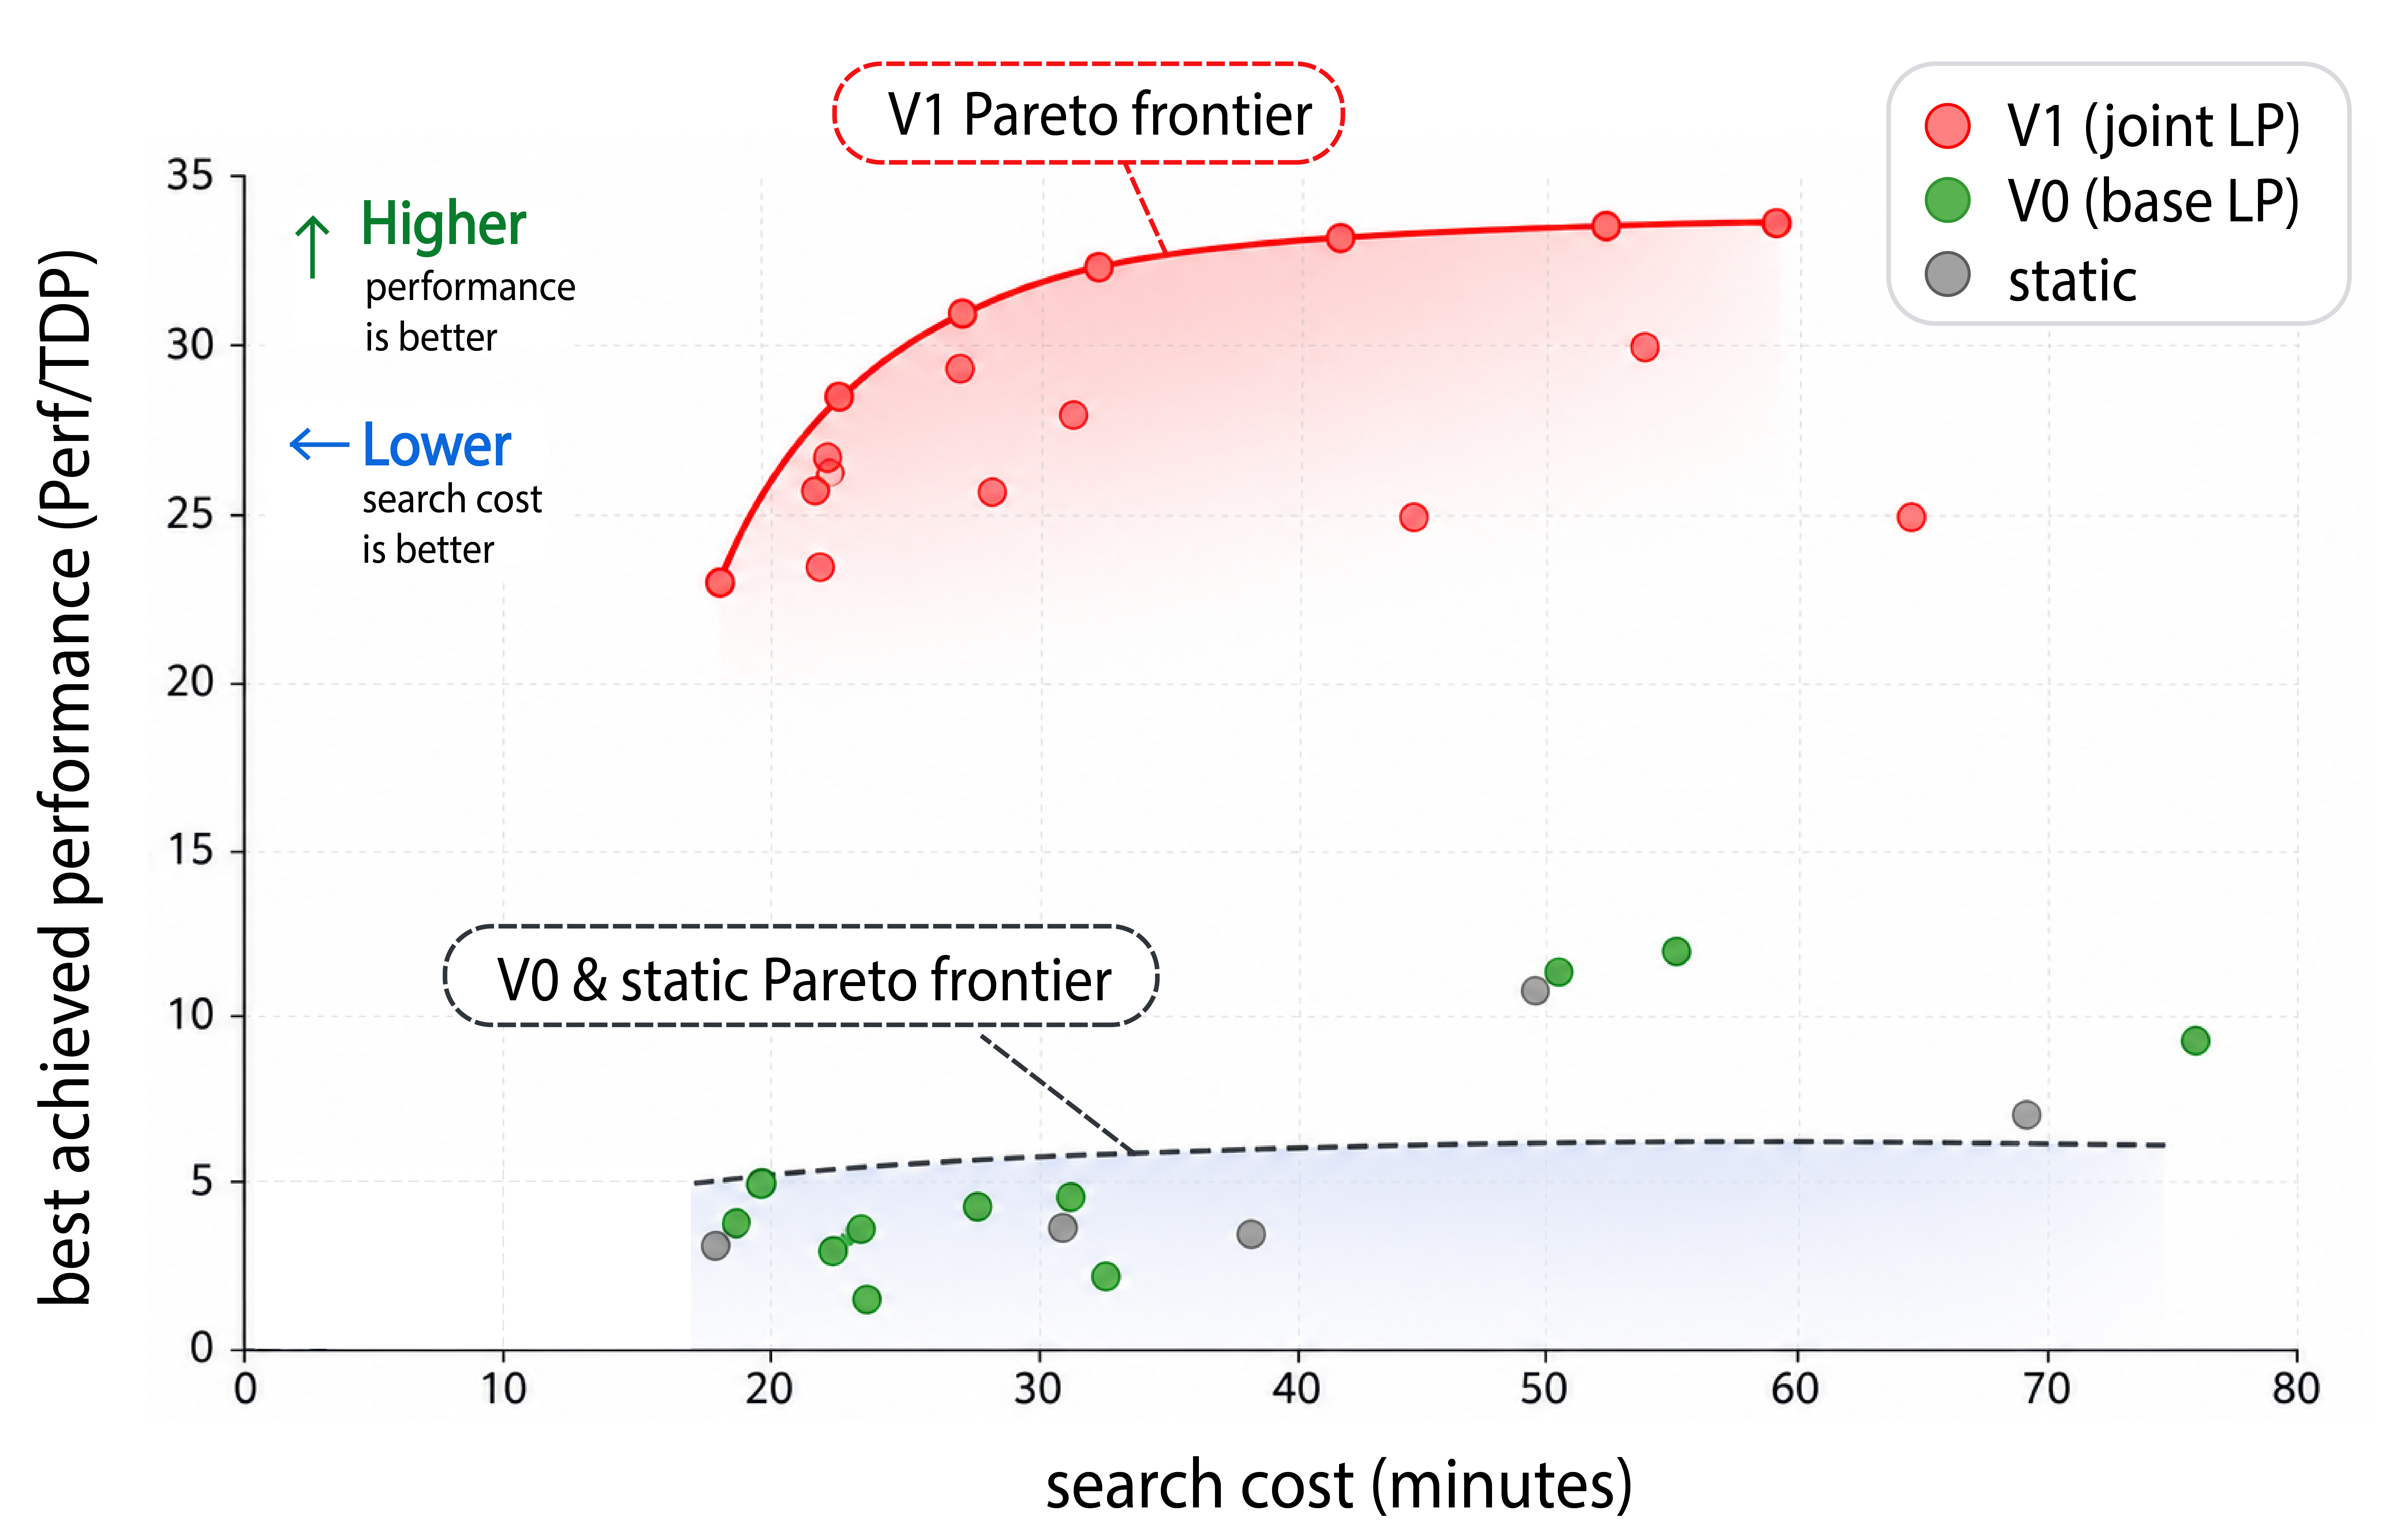
\includegraphics[width=0.7\linewidth]{figs/pareto_v2.png}
% %     \caption{pareto frontier plot}
% % \end{figure}
% \begin{figure}[ht!]
%     \centering
% 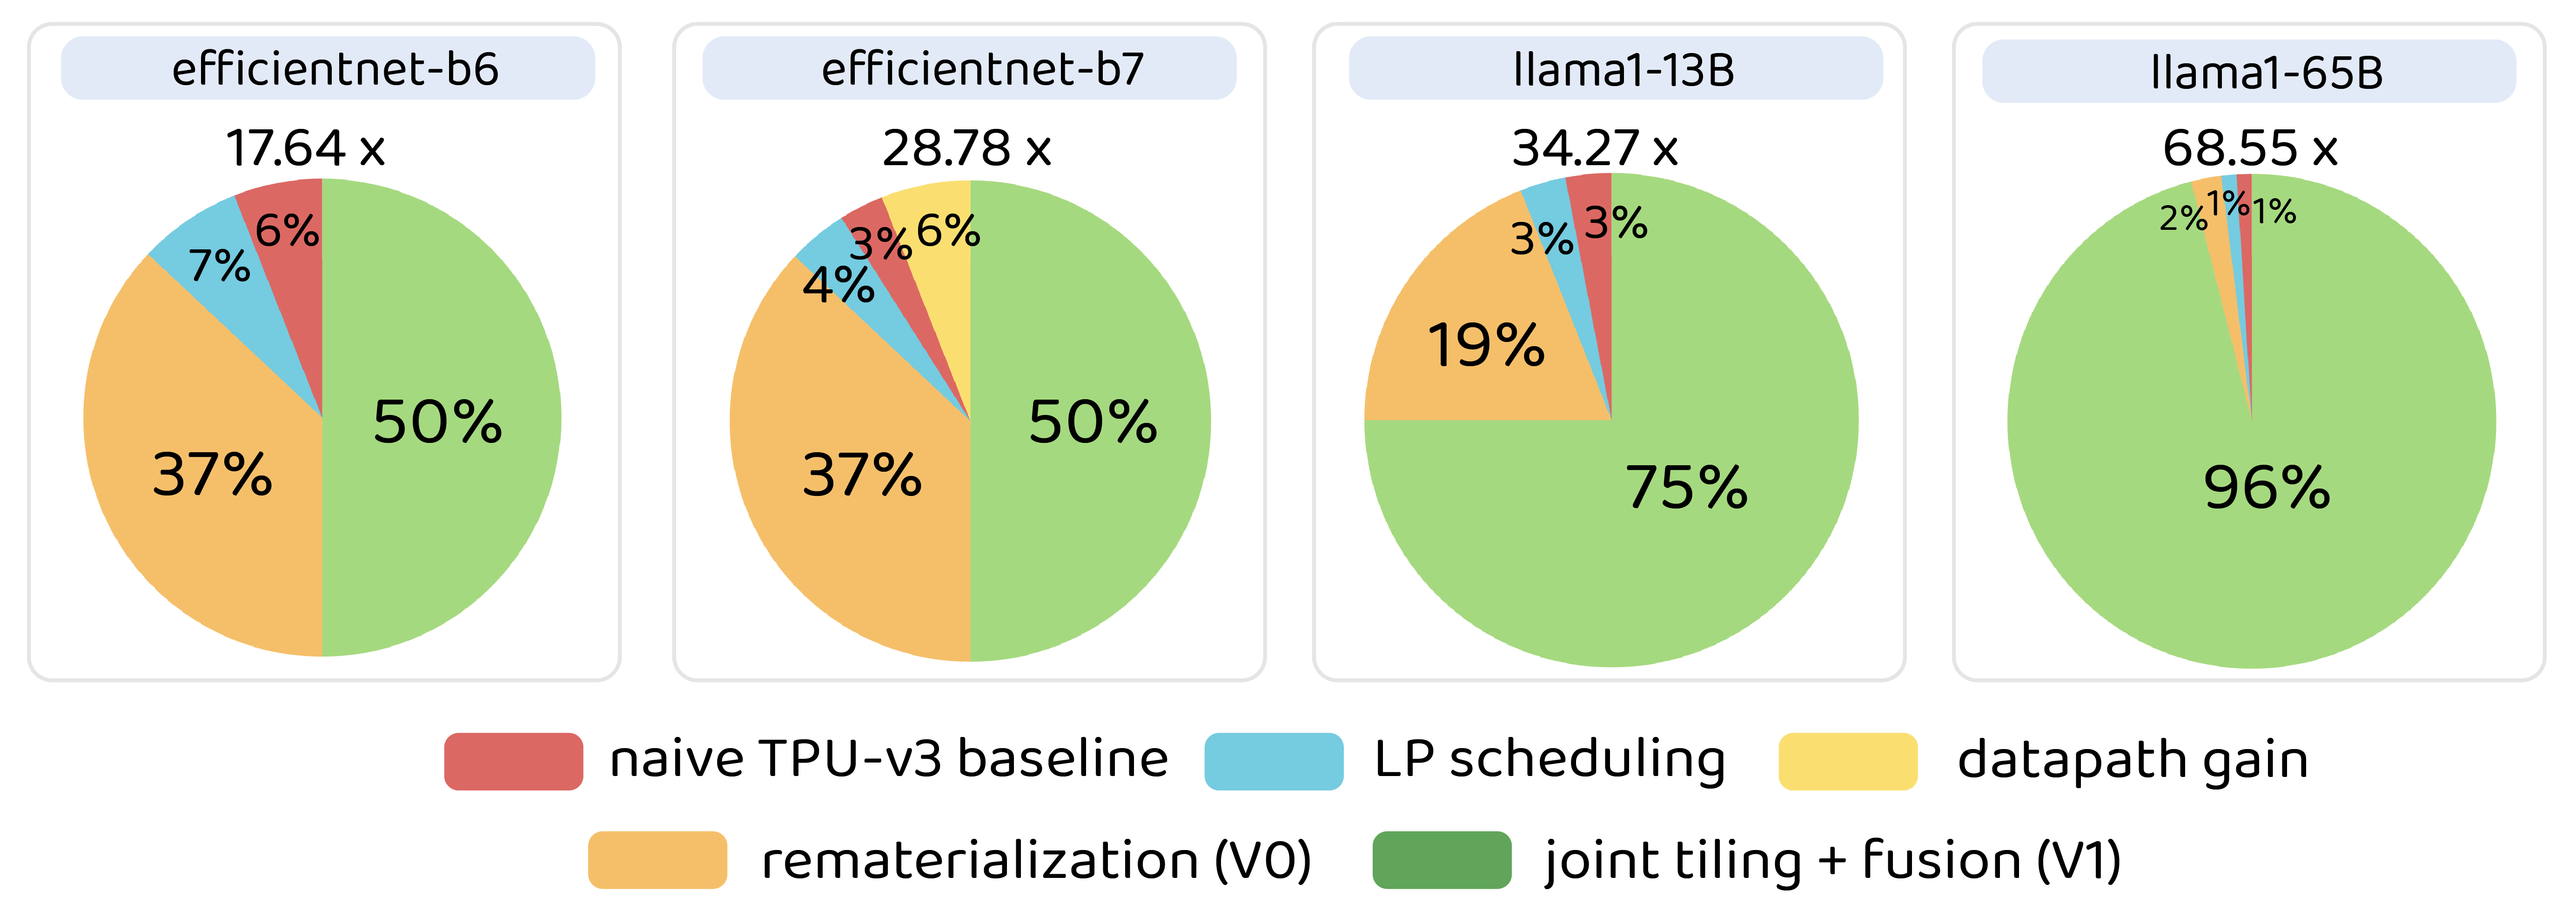
\includegraphics[width=0.85\linewidth]{fig3/speedup_decomposition_final_v2.png}
% \caption{Speedup decomposition over naive TPU-v3 baseline. Each pie shows the 
% relative contribution of four optimization sources to the total speedup. CHEETAH-V1 joint tiling + fusion dominates on all workloads, 
% especially on larger models where memory management is the primary bottleneck.}\label{fig:accel_decompose}
% \end{figure}
% \paragraph{CHEETAH-V0 vs.\ CHEETAH-V1 Unlock Progressive Gains.} Figure~\ref{fig:accel_decompose} decomposes the total speedup over a naive TPU-v3 baseline into four sources: LP-based scheduling and fusion, datapath gain from hardware search, dynamic rematerialization (CHEETAH-V0), and joint tiling + fusion (CHEETAH-V1).

% The dominant contributor across all workloads is V1's joint tiling-fusion 
% optimization. On EfficientNet-B1, V1 accounts for 50\% of total speedup, 
% with LP scheduling (28\%) and datapath gain (22\%) splitting the remainder---and 
% no rematerialization benefit, consistent with B1's small activation footprint 
% fitting comfortably in Global Memory. B3--B4 show a similar 50\% V1 share, but 
% V0 rematerialization now contributes 25\%, reflecting the growing value of 
% recomputing large depthwise activations rather than reloading them from DRAM. 
% From B5 onward, V1's share rises sharply to 75--88\%, as the increasing 
% model size makes joint tiling-fusion the primary lever: memory management 
% dominates, and the remaining sources (LP scheduling, V0, datapath) each shrink 
% to single-digit percentages. The same pattern holds on Llama, where V1 accounts 
% for 83--87\% of the total speedup.

% % \begin{wrapfigure}{r}{0.48\textwidth}
% %     \centering
% %     \vspace{-12pt}
% %     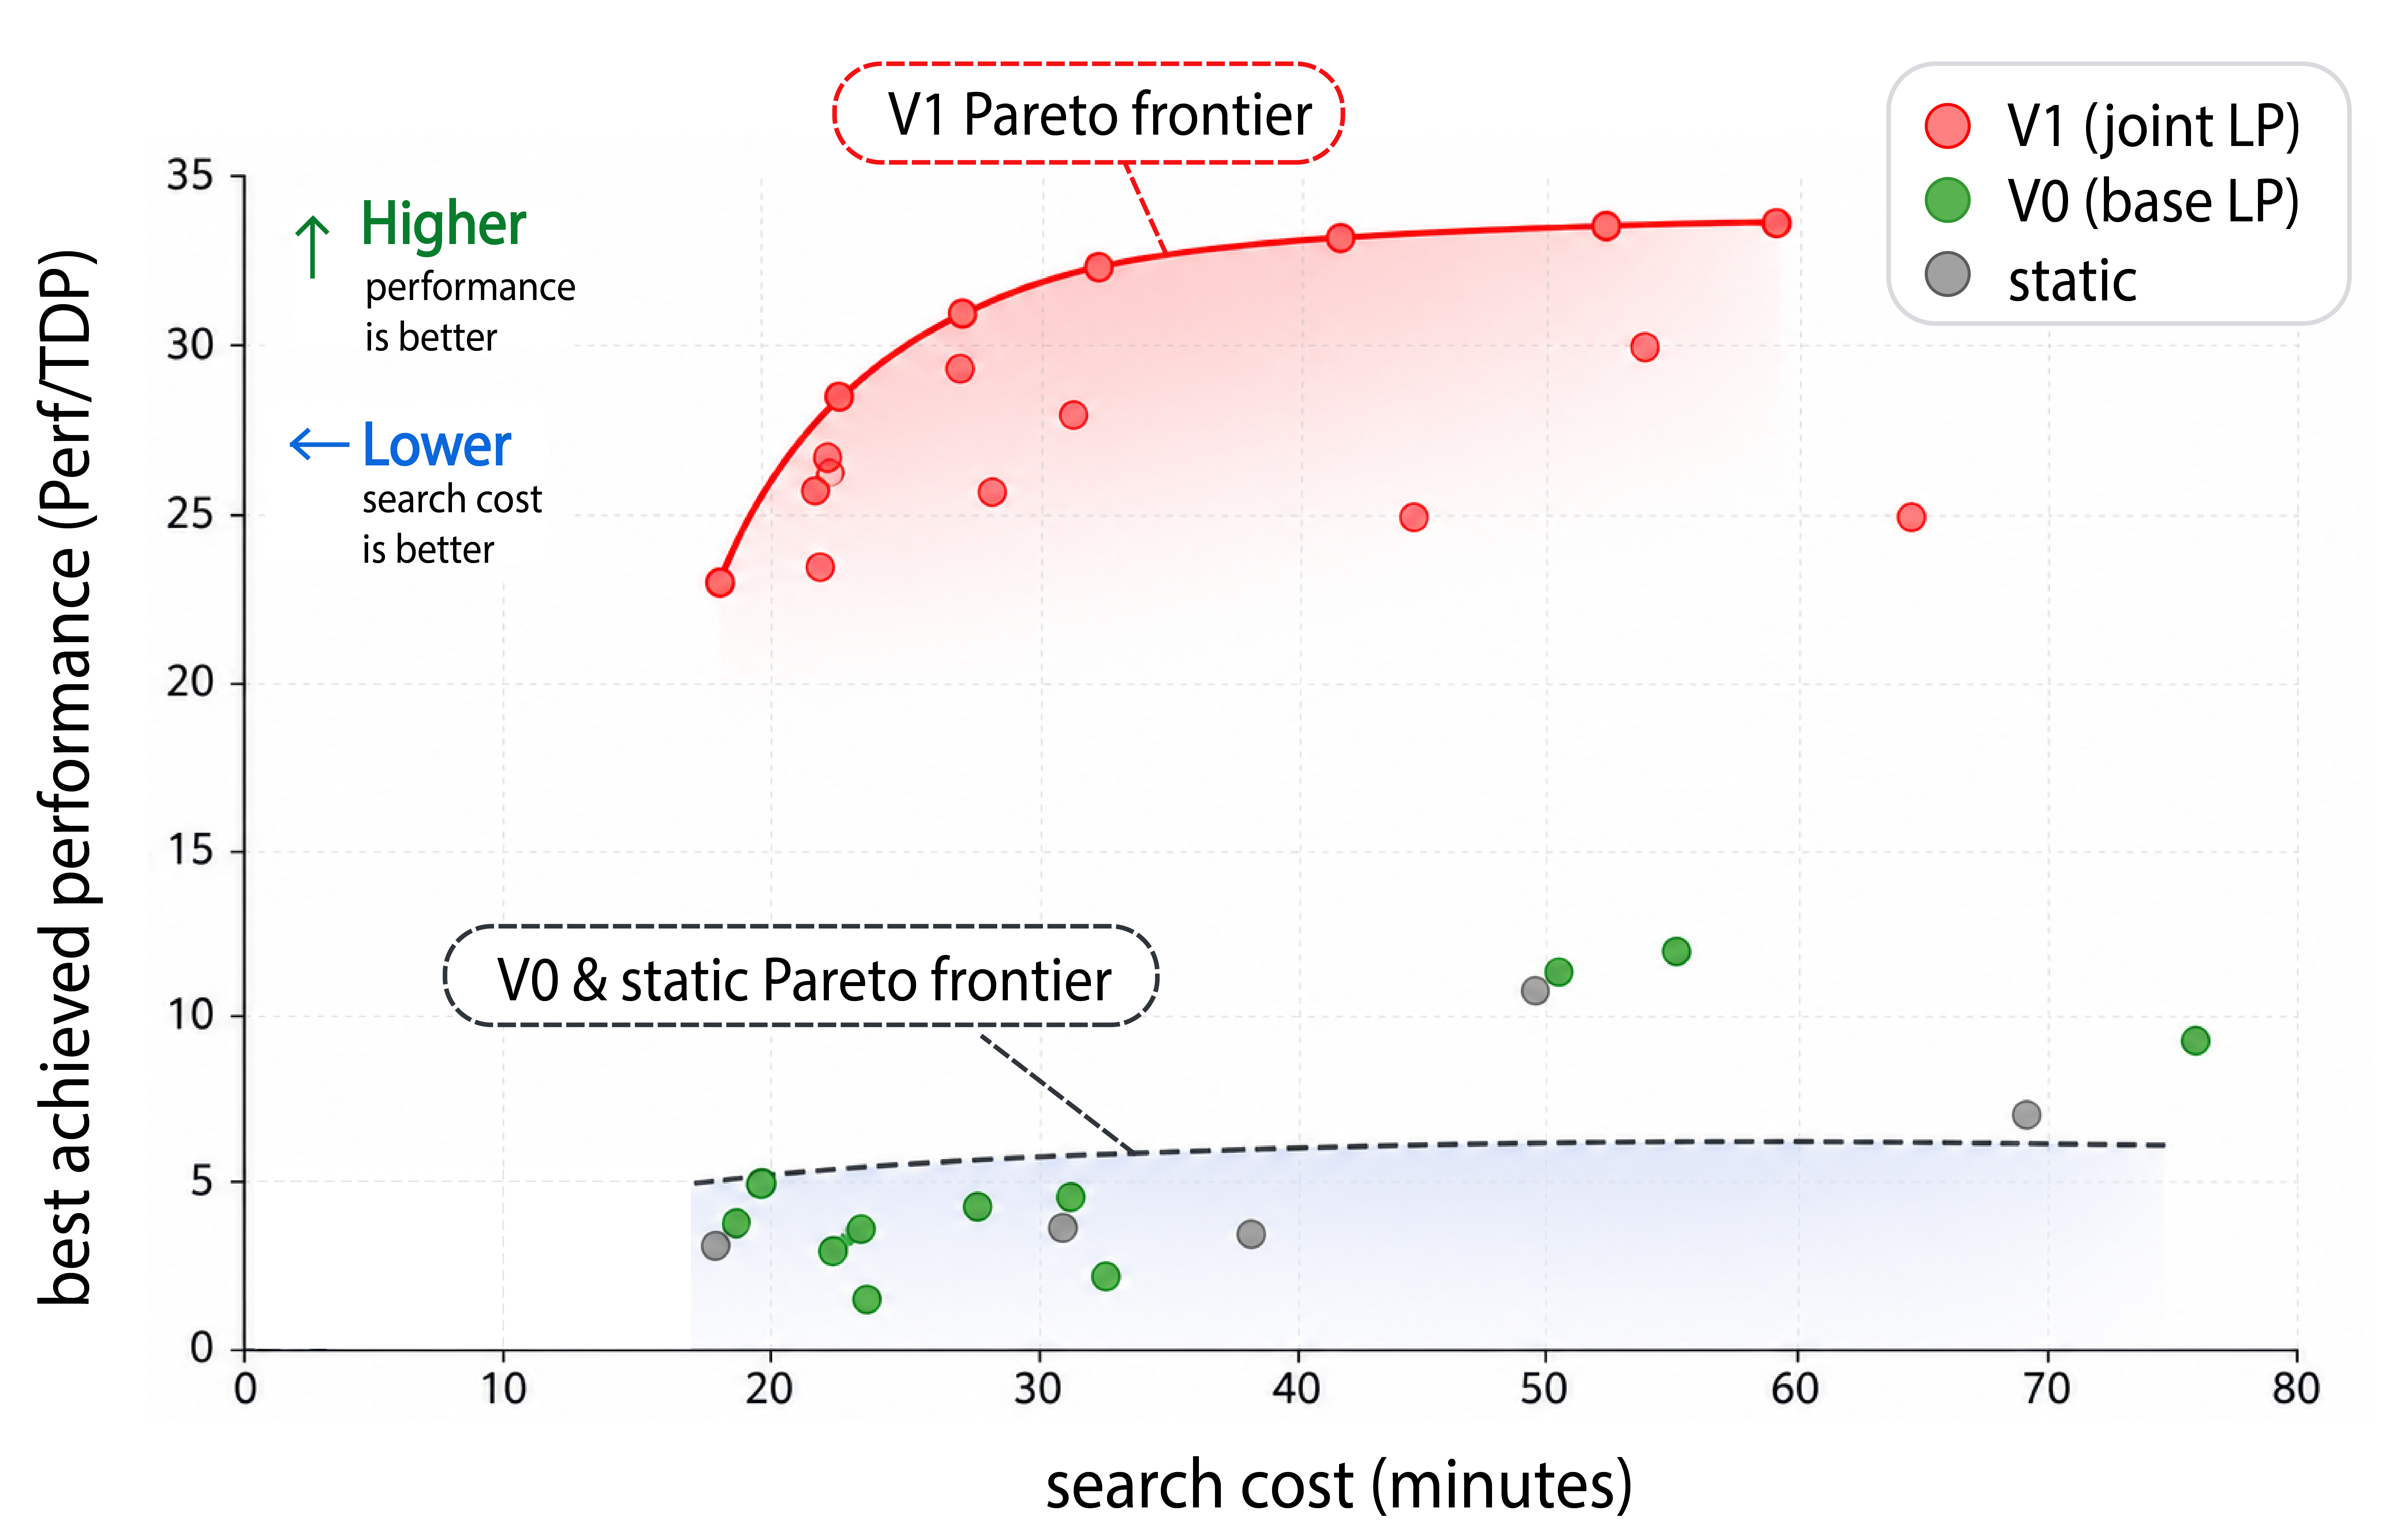
\includegraphics[width=0.48\textwidth]{figs/pareto_v2.png}
% %     \vspace{-18pt}
% %     \caption{Search cost vs.\ Perf/TDP Pareto frontier. V1 dominates V0 and static across all time budgets.}
% %     \label{fig:pareto}
% %     \vspace{-10pt}
% % \end{wrapfigure}

% Critically, Figure~\ref{fig:speedup} shows static fusion method is \emph{infeasible} on modern large models (Llama-70B, and DeepSeek-V3), because their large activation tensors cannot fit under a static pinning policy. The V0 formulation resolves feasibility for on large models via dynamic placement but remains time-intensive for a small number of 50 trials: measuring 58.42 hours on Llama-70B and 69.39 hours on DeepSeek-V3 (Figure~\ref{fig:wallclock}). In contrast Figures~\ref{fig:wallclock} and ~\ref{fig:speedup}, show the CHEETAH-V1 formulation out performs comparitive strategies in terms of speedup against the TPU-V3 baseline, and require only 1.17 hours on Llama-70B and 2.17 hours on DeepSeekv3 for 50 trails---a ${\sim}93\%$ average reduction. The powerful joint formulation is able to select memory-efficient tiling configurations alongside placement, achieving feasibility across the entire workload suite, demonstrating that joint optimization is not merely an incremental improvement but a qualitative capability unlock for large-scale models.

% % This demonstrates that by exploiting structural invariance and GPU-accelerated mathematical optimization, CHEETAH-V1 reduces the end-to-end co-design search time from days to under 2.2 hours—a ${\sim}93\%$ average reduction—while discovering architectural points that deliver up to $35\times$ speedup over the TPU-v3 baseline.

% % Figure~\ref{fig:pareto} shows the Pareto frontier of best-achieved Perf/TDP versus wall-clock search cost. V1 strictly dominates both V0 and static at every time budget: within 10 minutes of search, V1 already exceeds the best Perf/TDP that V0 or static achieve after 60+ minutes. The V1 Pareto frontier reaches ${\sim}35\times$ Perf/TDP, roughly $3\times$ higher than the V0/static frontier at ${\sim}10\text{--}12\times$. This gap reflects two compounding advantages: V1 explores a strictly larger feasible region (joint tiling-fusion), and it eliminates Timeloop from the per-trial critical path, allowing more trials within any fixed time budget.



% \paragraph{Practical insight.}
% Both LPs are extreme-aspect-ratio sparse: for \texttt{llama3\_70b},
% $m, n \sim 10^6$ and $\mathrm{nnz} \sim 5 \times 10^6$, giving roughly
% 1 nonzero per million matrix entries.
% The time-band structure means a coordinate-descent or stochastic PDHG
% solver would converge in $\mathcal{O}(T)$ sweeps if bands were the only
% structure.
% The capacity rows in both V0 and V1 LP formulations are the sole feature breaking strict banded structure, and they are precisely what couples the schedule globally. This is the desired behavior of a memory-aware placement formulation.

% % \todo{Report LP solve times for V0 and V1 across all benchmarks. Compare wall-clock time per trial against FAST's SCIP-based ILP solver (20 min timeout). Report LP relaxation gap: how often do fractional solutions need integer rounding, and what is the quality loss from rounding?}

% \paragraph{Structural invariance.}
% For a fixed workload and LP formulation, the LP constraint matrix
% has an invariant sparsity pattern across trials: the row/column
% dimensions and nonzero locations are determined only by the model graph structure — layer count $L$, timestep count $T$, edge set $E$, and Pareto count $C$ — not by the hardware candidate.
% Vizier changes only numerical values such as cycle coefficients,
% memory-capacity bounds, bandwidth-scaled access costs, objective weights, and TDP/area parameters. 
% This invariance allows us to reuse the same sparse matrix structure,
% variable ordering, block layout, and JIT-compiled sparse kernels in our adapted JAX PDLP solver across all hardware trials for a given workload. We apply the same diagonal preconditioning pipeline
% on each trial: a structural presolve with 20 log-geomean Ruiz iterations, followed by the PDLP preprocessing stack with 10 infinity-norm Ruiz iterations and one Pock--Chambolle $\ell_1$-scaling pass. This two-stage diagonal scaling handles the mixed coefficient magnitudes present in V0/V1 matrices — large byte-valued capacity rows together with $\pm 1$ persistence rows — without requiring a fragile matrix factorization. In production, this preconditioning pipeline is reused structurally across trials, recomputes only cheap diagonal scalings, finishes in under one second for matrices with approximately $5 \times 10^6$ nonzeros, and avoids factorization failures entirely because it consists only of $D_1 A D_2$ arithmetic.

% \paragraph{LLM Architect vs.\ Optimizer.} 
% \begin{wrapfigure}{r}{0.50\textwidth}
%     \centering
%     \vspace{-6pt}
%     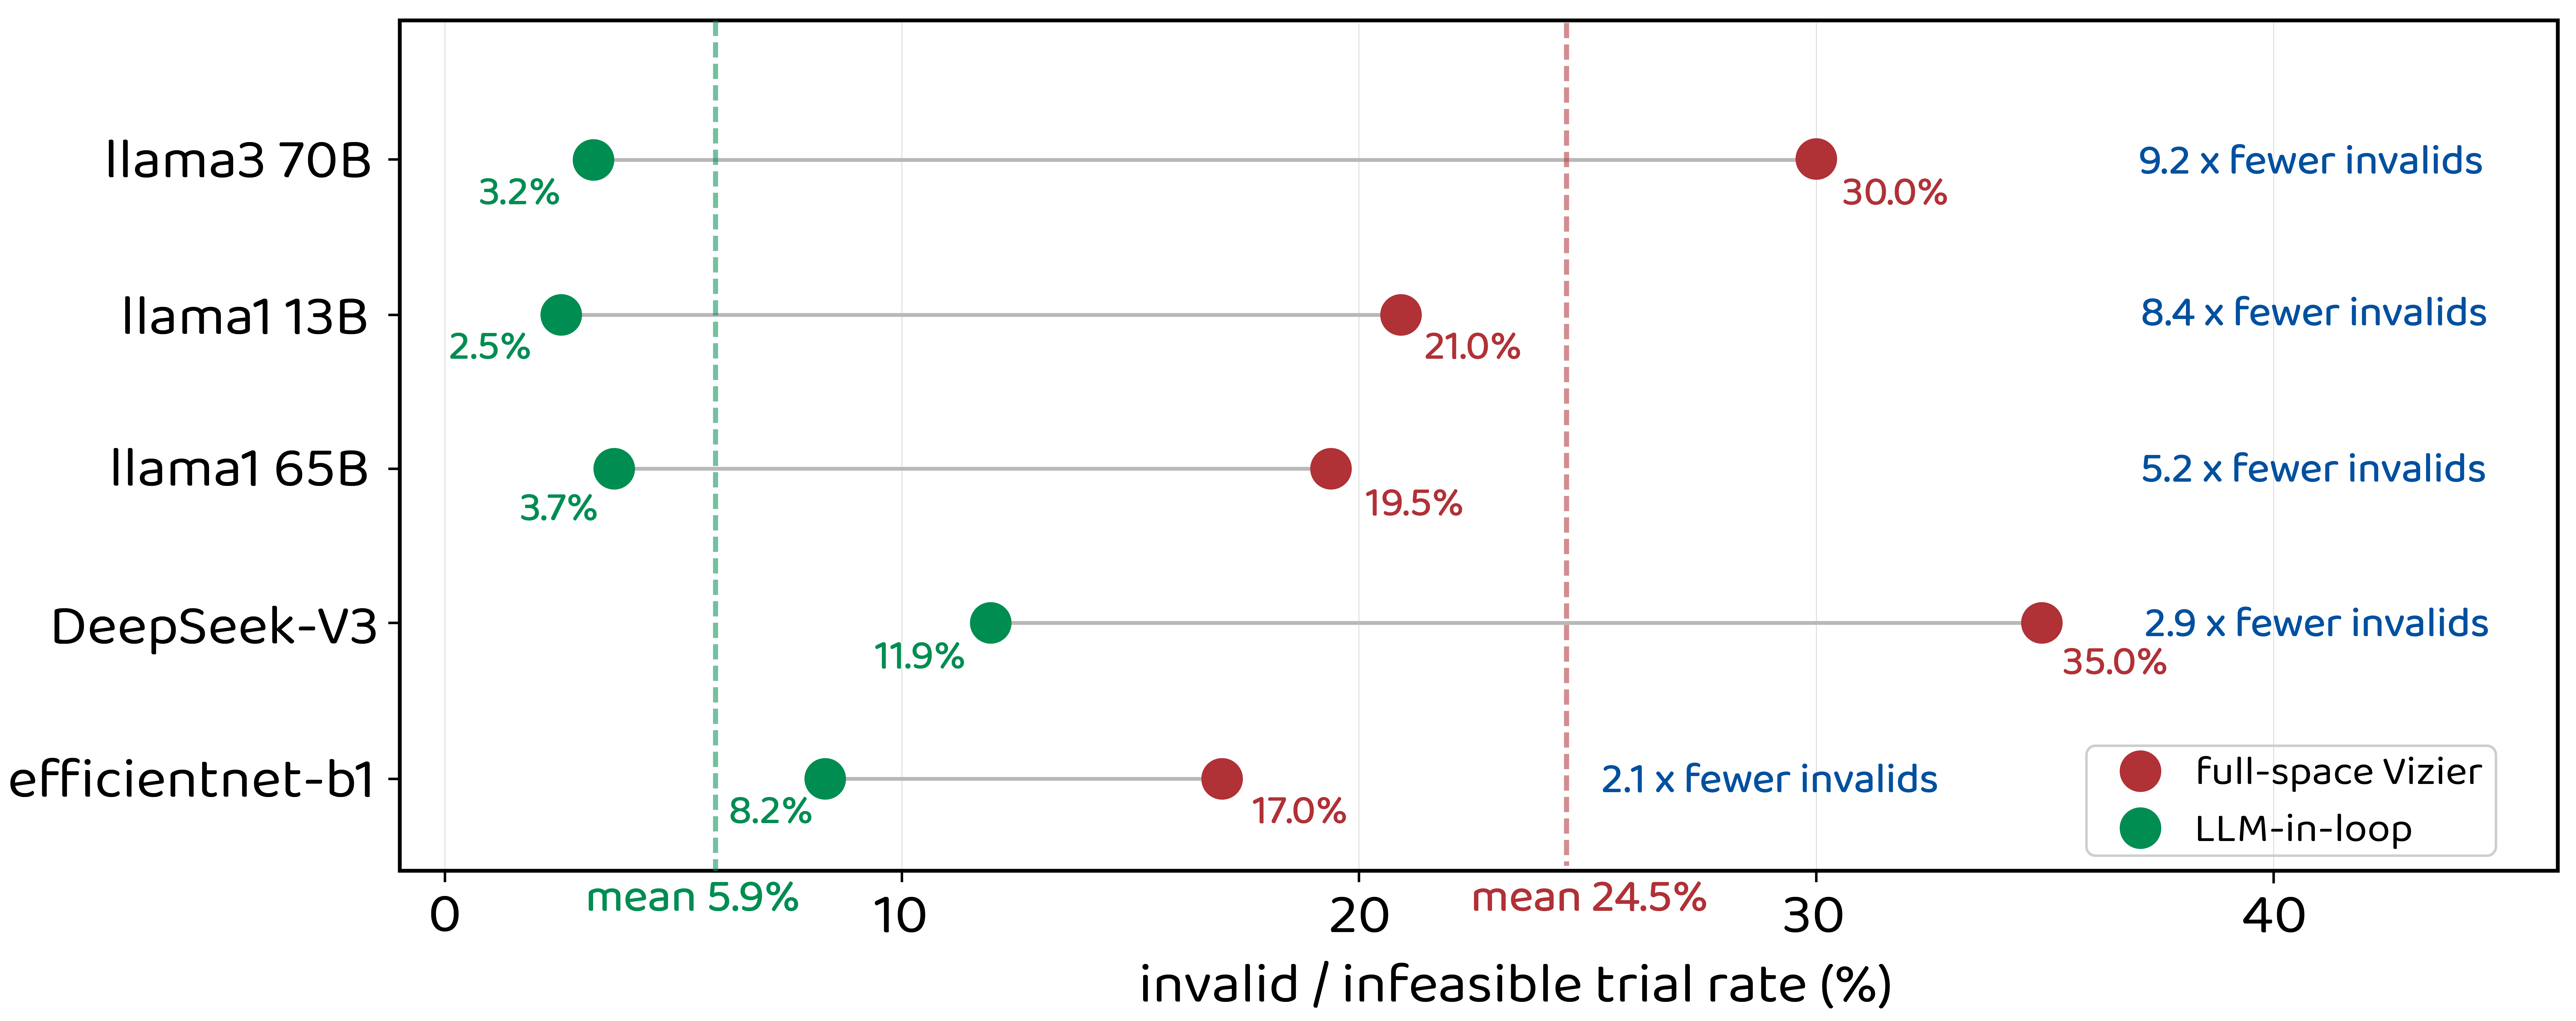
\includegraphics[width=0.48\textwidth]{fig3/llm_guide_v1.png}
%     \caption{Strategic Intelligence vs.\ Stochastic Brute Force. Green indicates the LLM-Architect has less wasted trials.}
%     \label{fig:llm}
%     \vspace{-10pt}
% \end{wrapfigure}

% Modelled on SkyDiscovery~\citep{skydiscover2026}, the LLM Architect prunes
% the outer search loop by proposing campaign patches rather than
% predicting raw performance. It analyses a Causal Ledger containing
% invalid rates, MFU, and solver diagnostics to suggest constrained
% hardware neighbourhoods for Vizier to explore locally. The V1 LP
% remains the ground-truth evaluator, supported by a Roofline Auditor
% that rejects physically impossible results.
% In a widened search space, the LLM loop reduces invalid evaluations
% from $24.5\%$ to $5.9\%$ on average — a $4.1\times$ reduction in wasted
% trials — while reaching the same optimal Perf/TDP scores as full-space
% Vizier. This demonstrates that the LLM's role is steering Bayesian
% optimisation toward feasible, workload-appropriate subspaces rather than
% replacing the solver. This framework establishes a foundation for
% integrating complex human reasoning into the co-design loop.

% % \subsubsection{LLM Architect vs. Optimizer}
% % The LLM Architect framework is modeled on SkyDiscover, and efficiently prunes the large outer hardware search loop by proposing campaign patches. Rather than predicting performance, the Architect reads a compact Causal Ledger containing invalid-rate history, MFU, roofline lower-bound checks, and LP diagnostics, then proposes a constrained hardware neighborhood for Vizier to search locally. The V1 LP remains the sole performance evaluator: for each candidate, it solves the joint tiling, fusion, placement, and rematerialization LP, while a deterministic Roofline Auditor rejects physically impossible results. In the widened V1 search space, all methods reach the same capped V1 Perf/TDP ceiling, so the key differentiator is search efficiency. The LLM loop reduces invalid hardware evaluations from 24.5\% under full-space Vizier to 5.9\% on average across five workloads, a 4.1× reduction in wasted trials, while preserving the same best V1 score. This shows that the LLM’s contribution is not replacing Vizier or the solver, but steering Bayesian optimization toward feasible, workload-appropriate architectural neighborhoods with far less wasted trials. This also sets the foundation for future work, where the LLM in the loop can adhere to follow more complex human reasoning signals.
% % \begin{figure}[ht!]
% %     \centering
% % 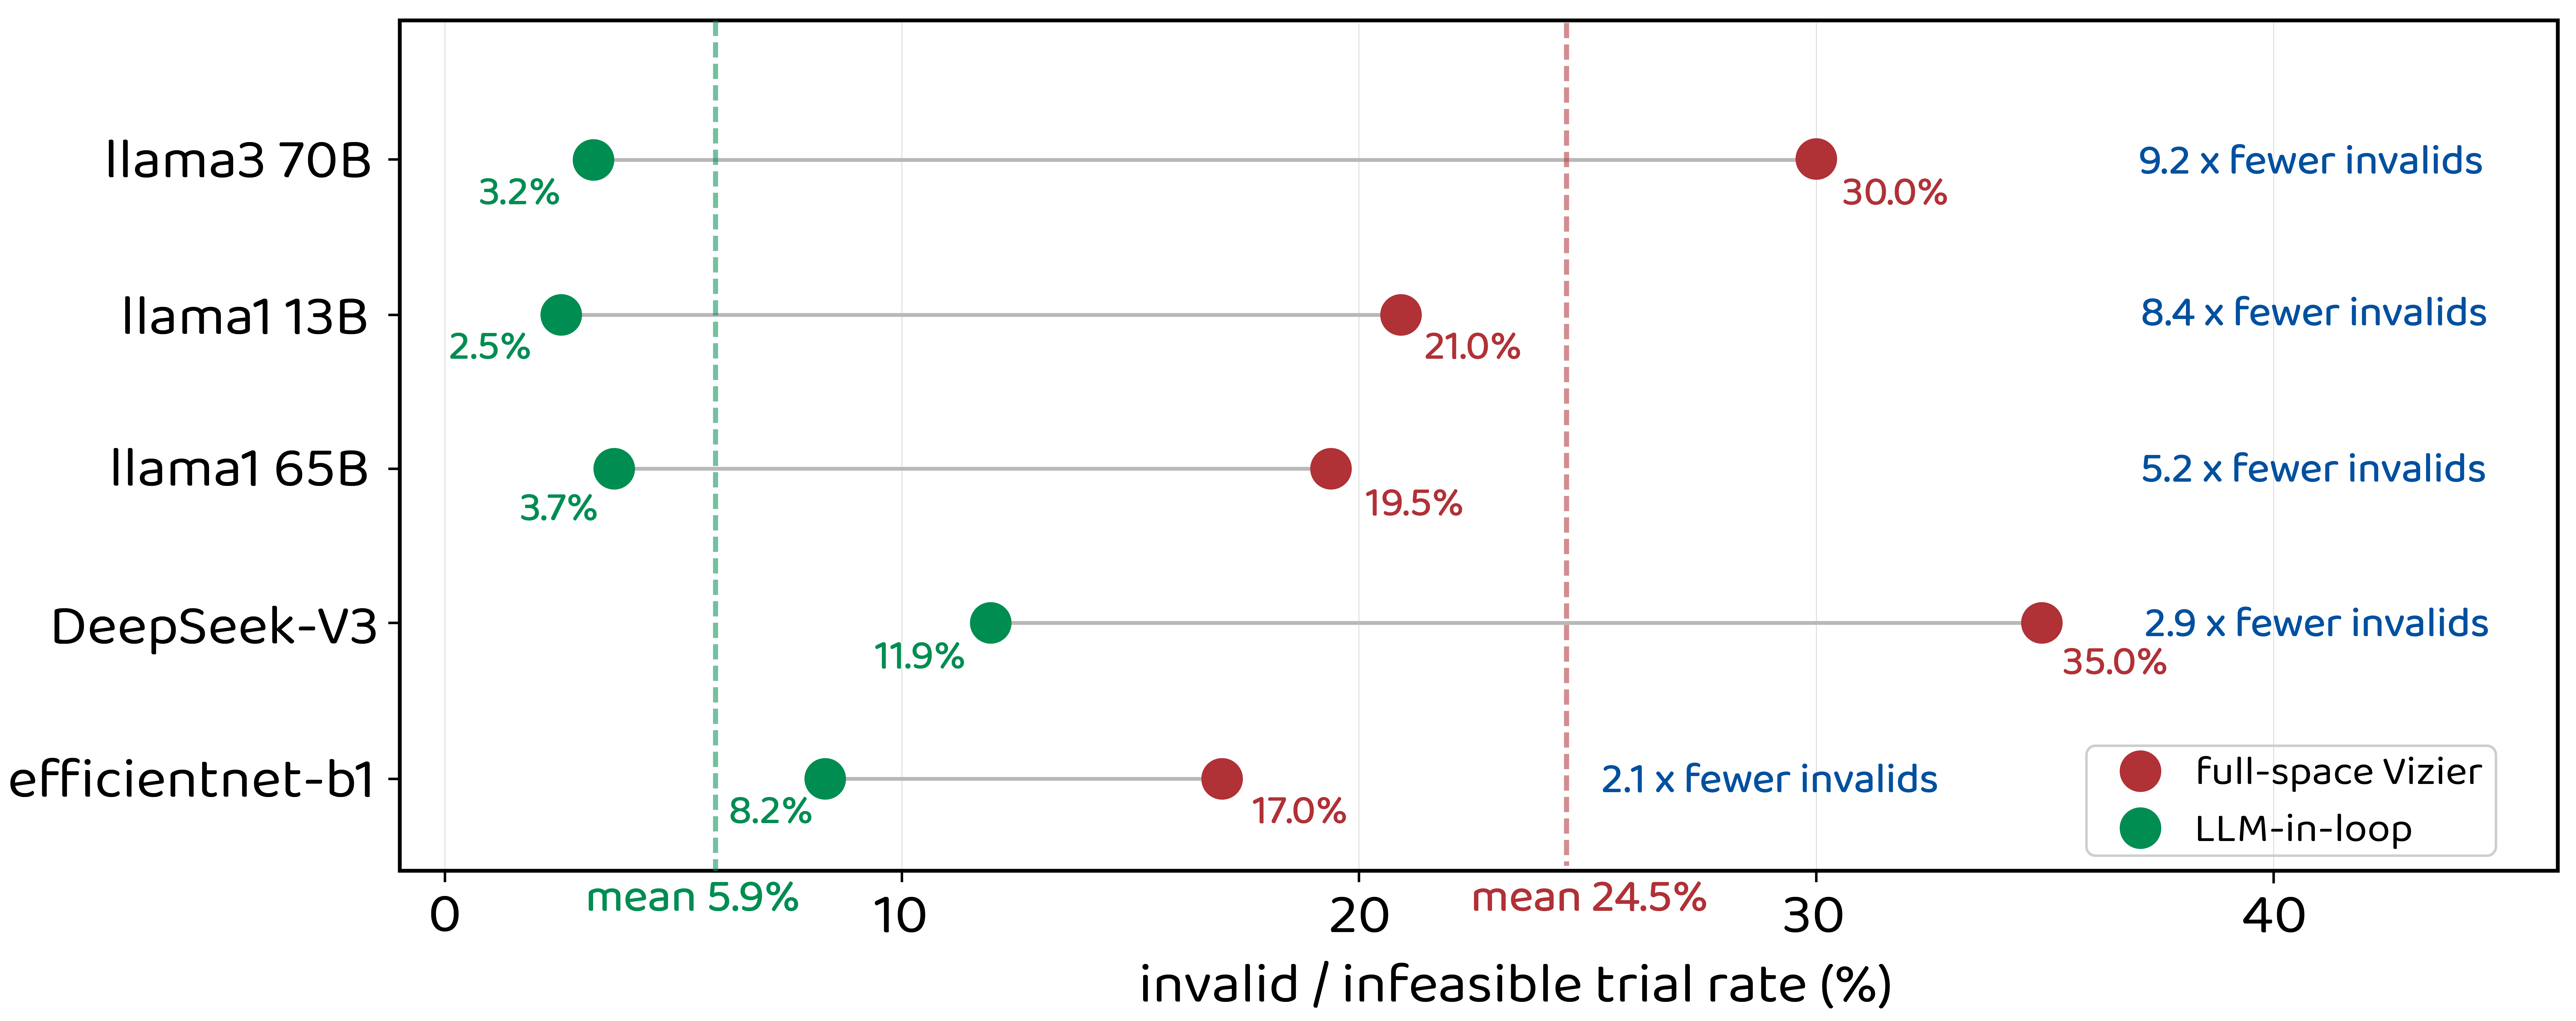
\includegraphics[width=0.85\linewidth]{fig3/llm_guide_v1.png}
% % \caption{Strategic Intelligence vs. Stochastic Brute Force}\label{fig:llm}
% % \end{figure}



% % The LLM should not just ask, “What chip has the best Perf/TDP?” We aim to answer the question “Given this user’s workload and deployment goal, what is the architectural region to search for this deployment task?”. Therefore we have the LLM emit profile-conditioned campaigns that take specific user inference tasks into consideration. For each $(\text{deployment profile},\ \text{workload})$ cell, we ran a
% % 200-trial LLM-Architect experiment using the same Qwen2.5-7B-Instruct + LoRA with differing user input profiles. At the start of each round, the prompt was assembled from a fixed system
% % prompt, the active deployment profile, three few-shot examples, and a per-round user message containing the workload, recent feedback signals, current search bounds, and the causal ledger.
% % The Strategist returned a one-line JSON campaign patch, which the
% % validator accepted only if it was a strict legal subset of the parent space, satisfied hard rules such as patch-volume $\leq 10\%$, ridgepoint and MAC/BW constraints, and avoided forbidden regions.

% % Thus, the experiment isolates whether the profile-conditioned LLM prompt alone can steer the same V1 evaluator toward different hardware families under different deployment intents.



% % \todo{Compare convergence rate of LLM-guided hardware search vs.\ Vizier-only (Bayesian, LCS, random baselines) in the style of FAST Figure~11. Report:
% % \begin{itemize}
% %     \item Number of trials to reach $X\%$ of best Perf/TDP found by 5,000-trial Vizier
% %     \item Quality of LLM-proposed configurations vs.\ Vizier-proposed configurations
% %     \item Qualitative analysis of LLM reasoning about hardware bottlenecks
% % \end{itemize}
% % }

% % \subsubsection{ROI Analysis}

% % \todo{Update FAST's ROI analysis (Table~4) with the improved Perf/TDP numbers from FAST-CORGI. Report deployment volumes required to reach 1$\times$, 2$\times$, 4$\times$ ROI targets. If Perf/TDP improvements are larger than FAST's, the break-even deployment volume should decrease correspondingly.}

% % \subsubsection{Pareto Frontier}

% % \todo{Plot the Perf/TDP vs.\ area Pareto frontier for V1-optimized designs compared to FAST and TPU-v3 baseline, analogous to FAST Figure~12.}

% page edit

% \section{Experiments}
% \label{sec:experiments}
% In all cases we use an adapted JAX PDLP solver for large models at LLama70-B and DeepSeekv3 scale across all three methods (Static, CHEETAH-V0, CHEETAH-V1); and use HiGHS as the default solver for all other smaller neural network models. In order to be consistent with prior work, our experimental results are presented as orders of speedup / performance against a vanilla TPU-V3. This is also since TPUs are targeted for NN accelerators (as opposed to GPUs), and the TPU-V3 has the most information publically released, making it possible for us to simluate it more accurately. 

% \subsection{Experimental Setup}

% \paragraph{Static Sequential Baseline.}
% We compare against the static optimization FAST framework using a simulated TPU-v3 baseline normalized to a sub-10nm process technology, following the same methodology as Zhang \etal. The baseline simulator is well-correlated with production hardware: on average within 8.2\,$\pm$\,2.7\% of profiled TPU-v3 performance. We evaluate against a \emph{simulated} TPU-v3 baseline to account for optimistic simulator assumptions.

% We evaluate across 11 representative workloads: EfficientNet-B1 through EfficientNet-B7, Llama13, 65, 70 models, and DeepSeek-V3-MoE. These workloads stress different parts of the hardware design space: EfficientNet stresses low-operational-intensity depthwise convolutions, while Llama and DeepSeek stress memory capacity, bandwidth, and large matrix operations. 

% \textbf{Single-workload specialization.} Each neural network workload is optimized independently. This experiment measures the best workload-specific hardware found under a fixed trial budget and identifies architectural preferences such as Global Memory size, bandwidth, MAC count, and systolic shape. In the case of Staitic and V0 methods, the pipeline involves: Vizier - Timeloop - LP solver. In the case of the V1 method, the pipeline is simplified to Vizier - LP solver. In each case we iterate for 100 trials per method x NN. 

% % \textbf{Fixed-hardware-workload generalization.} We search for general-purpose datapaths that perform well across the workload suite. The objective is a harmonic or geometric aggregation of per-workload Perf/TDP, forcing the search to balance CNN-style memory pressure and LLM-style compute/memory trade-offs.

% \textbf{LLM-Architect guides outer search.} We the LLM-guided outer-loop controller which proposes search-space interventions for Vizier. The advantage of the CHEETAH-V1 formulation is it removes dependence of Timeloop in the loop. Therefore the loop is reduced to just Vizier-LP solve, which dramatically speeds up the iterative process, thus permitting the LLM-Architect outer loop. The LLM is only permitted to change the search neighborhood of Vizier's input, the strict LP formulation on the inner loop does not change. This ensures mathematical and physical constraints are upheld in the space of co-design. 

% % \paragraph{Optimization framework.}
% % For the outer hardware search loop, we use Google Vizier with LCS optimization and safe search, running 100 trials per experiment (method X NN x Exp). Each trial invokes the LP solver for the inner optimization. The Static and V0 methods additionally have Timeloop in the loop (Vizier-Timeloop-LP solve). The advantage of the v1 formulation is it removes dependance of Timeloop in the loop. Therefore the loop is reduced to just Vizier-Lp solve, which dramatically speeds up the iterative process, thus permitted the Strategic LLM outer loop.

% We validate our framework through a multi-level audit process to ensure physical and numerical rigor.
% \textbf{Roofline Auditor.}
% A deterministic Roofline Auditor enforces physical feasibility by
% verifying that LP-predicted latencies never fall below the theoretical
% bound
% \begin{equation}
%     \mathrm{LB} = \max\!\left(t_{\mathrm{compute}},\;
%     t_{\mathrm{memory}}\right),
%     \label{eq:roofline_lb_val}
% \end{equation}
% where $t_{\mathrm{compute}}$ and $t_{\mathrm{memory}}$ represent the
% peak compute and memory bandwidth floors, respectively.
% All reported V0/V1 results are roofline-feasible with valid
% $\mathrm{MFU}_{\mathrm{bound}}$ and memory utilization metrics.

% \textbf{Campaign Validator.}
% A deterministic Campaign Validator legalizes LLM-proposed architectural
% neighbourhoods by enforcing hard hardware constraints — including TDP
% caps, area limits, and power-of-two parameter ranges — prior to Vizier
% sampling.

% \textbf{Causal Ledger.}
% A Causal Ledger tracks LLM interventions and observed outcomes,
% preventing redundant exploration of empirically invalid regions and
% ensuring full auditability of the search loop.

% \textbf{Solver Diagnostics.}
% We monitor solver diagnostics including primal/dual residuals, duality
% gap, and rounding gap. Designs are treated as trustworthy only when both
% the continuous LP relaxation and the rounded integer solution are
% numerically well-behaved.


% \subsection{Main Results}

% % \subsubsection{V0 vs.\ FAST Static Fusion}

% % \todo{Insert results table and figure comparing V0 (time-indexed placement + rematerialization) against FAST's static fusion ILP on all benchmarks. Key metrics: Perf/TDP improvement, fusion efficiency (\% of DRAM stall time eliminated), rematerialization frequency (how often does the solver choose to recompute rather than reload?).}

% % \paragraph{Expected findings.}
% % V0's dynamic placement should show the largest gains on workloads with: (1)~tight Global Memory budgets where static pinning wastes capacity on tensors that are only needed briefly, (2)~long dependency chains where tensor lifetimes vary substantially, and (3)~cheap-to-recompute operations with large activations (\eg, depthwise convolutions in EfficientNet).

% % \subsubsection{V1 vs.\ V0: Joint Tiling and Fusion}

% % \todo{Insert results table and figure comparing V1 against V0 on all benchmarks. Key metrics: Perf/TDP improvement, number of operations where V1 selects a different tiling configuration than Timeloop's greedy choice, and the resulting compute efficiency vs.\ fusion trade-off.}

% % \paragraph{Expected findings.}
% % V1 should show the largest gains on architectures with highly diverse layer types where a single tiling configuration cannot serve all operations well. EfficientNet (depthwise + pointwise convolutions with 100$\times$ variation in working-set sizes) and hybrid CNN-transformer models (convolutions + attention + MLP with fundamentally different compute-memory profiles) are expected to benefit most.


% % \subsubsection{stiatic vs v0 vs v1}
% % \begin{figure}[ht!]
% %     \centering
% %     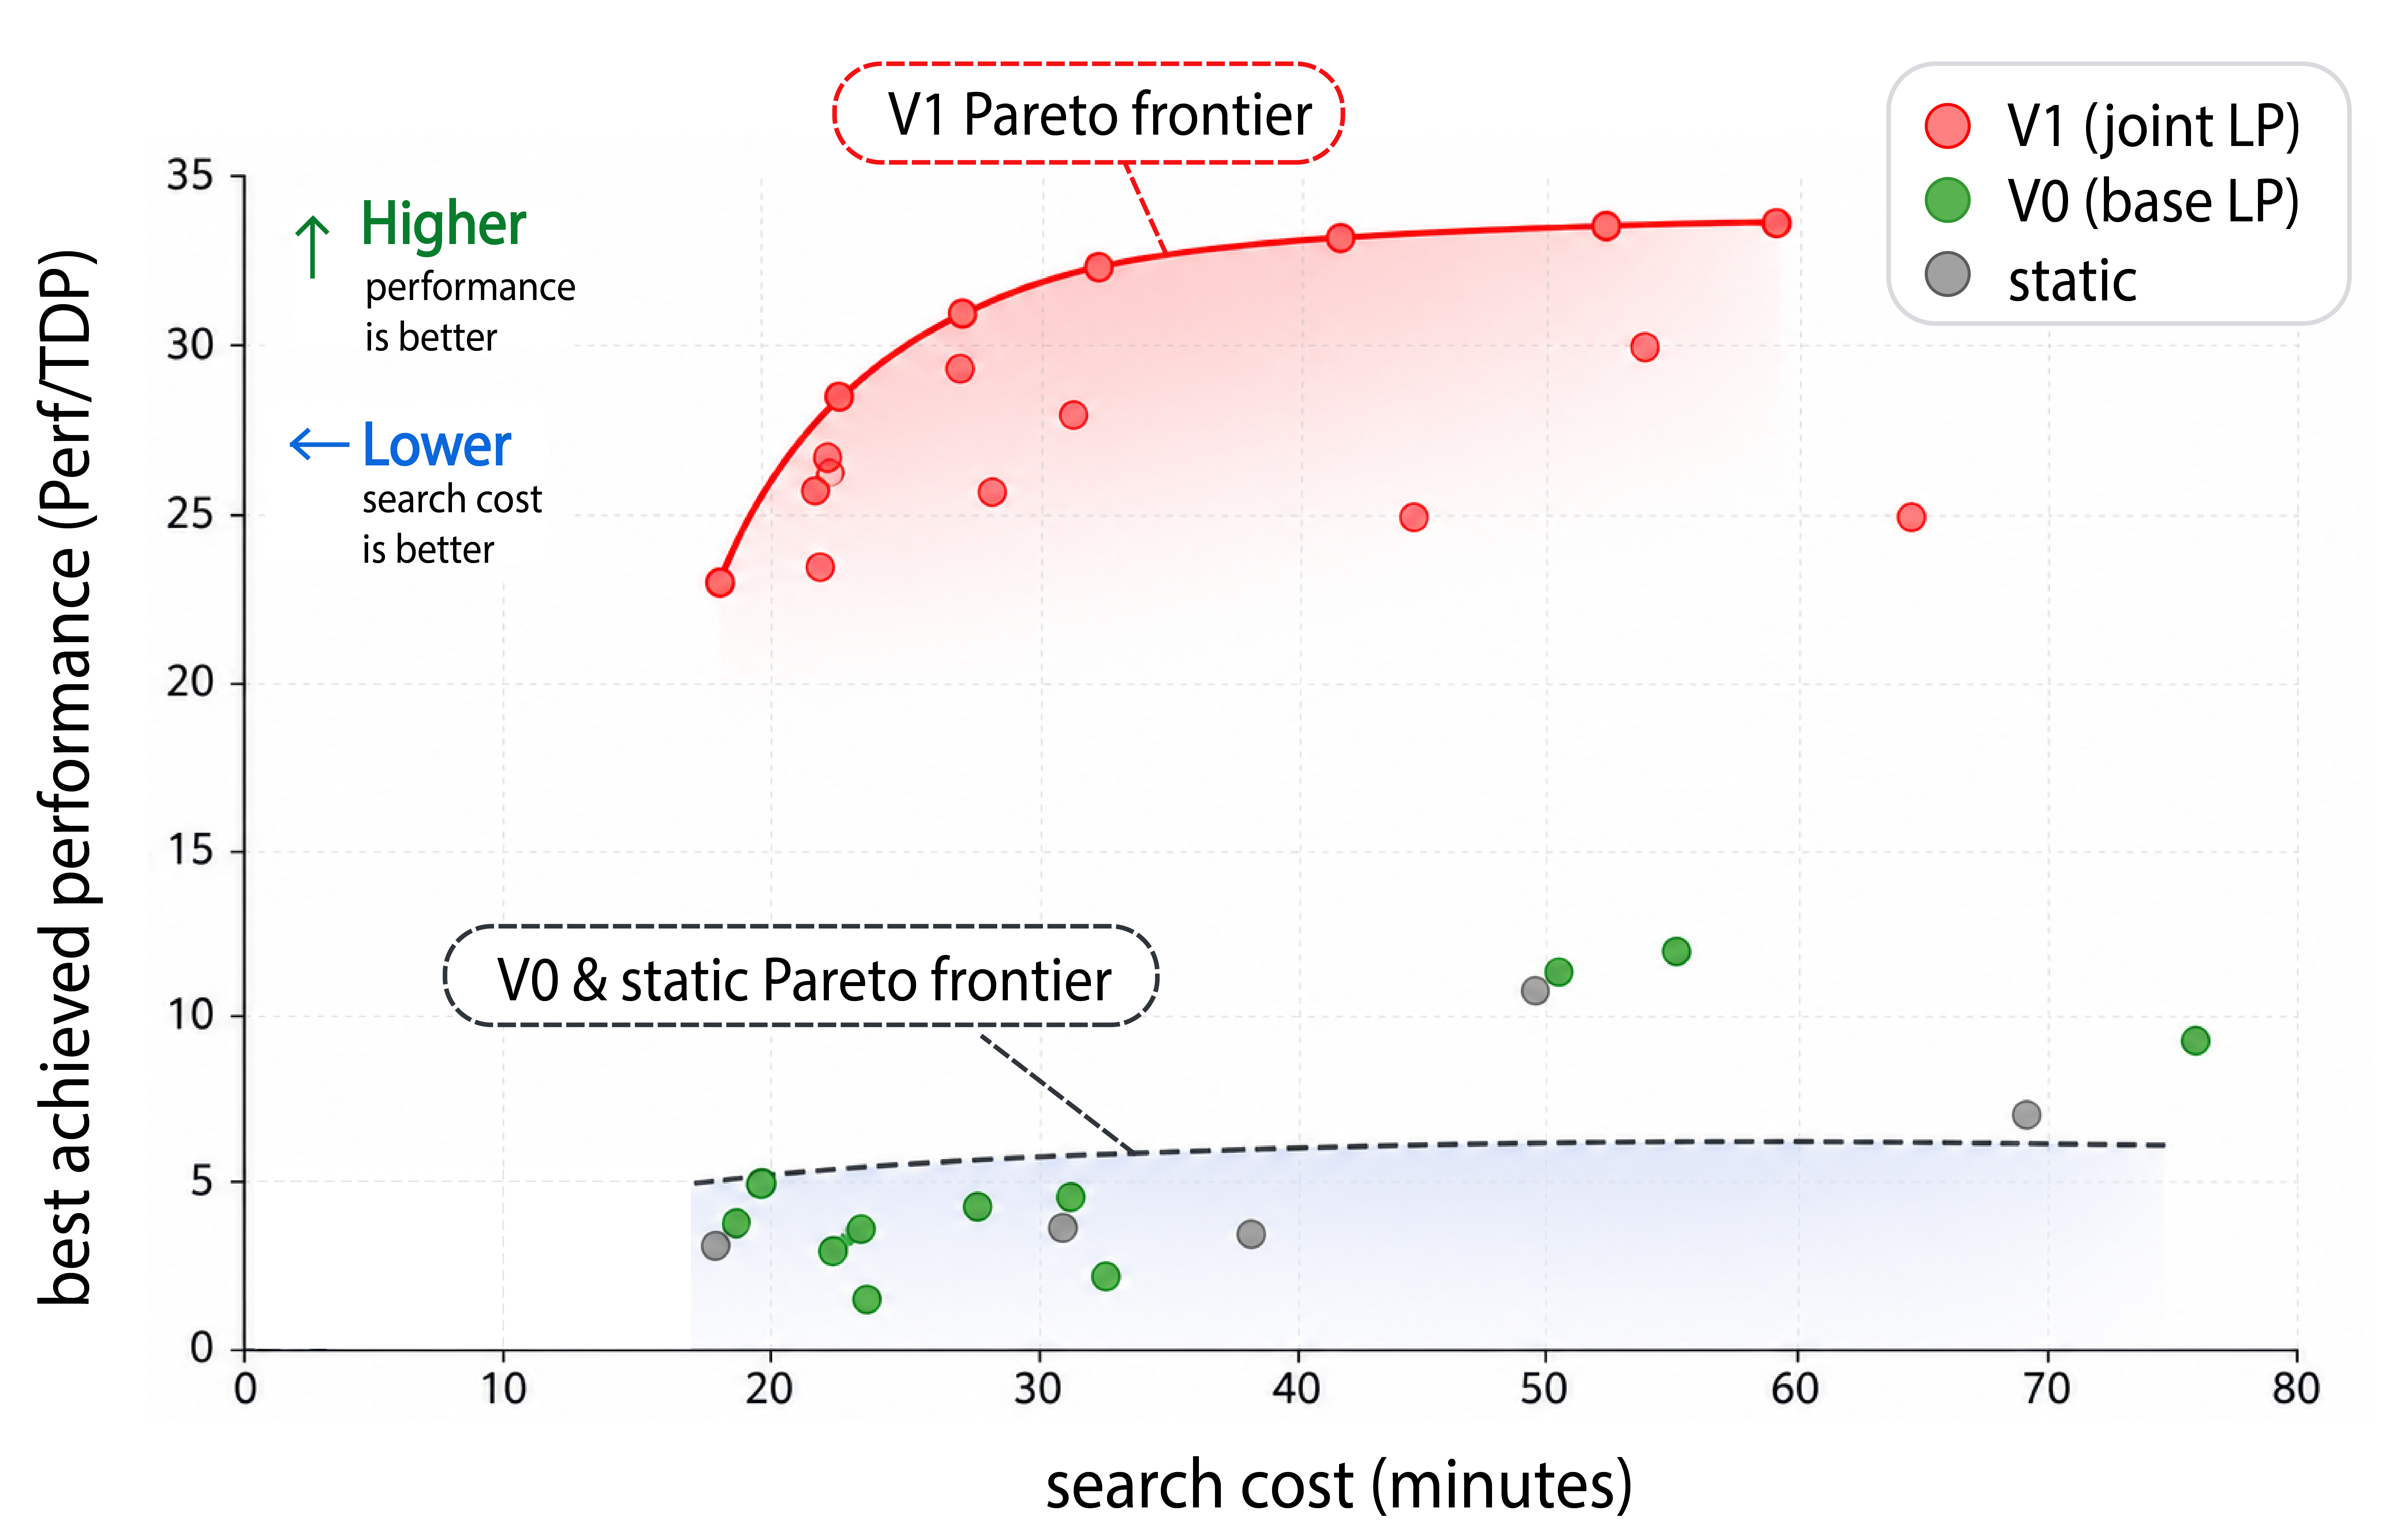
\includegraphics[width=0.7\linewidth]{figs/pareto_v2.png}
% %     \caption{pareto frontier plot}
% % \end{figure}
% \begin{figure}[ht!]
%     \centering
% 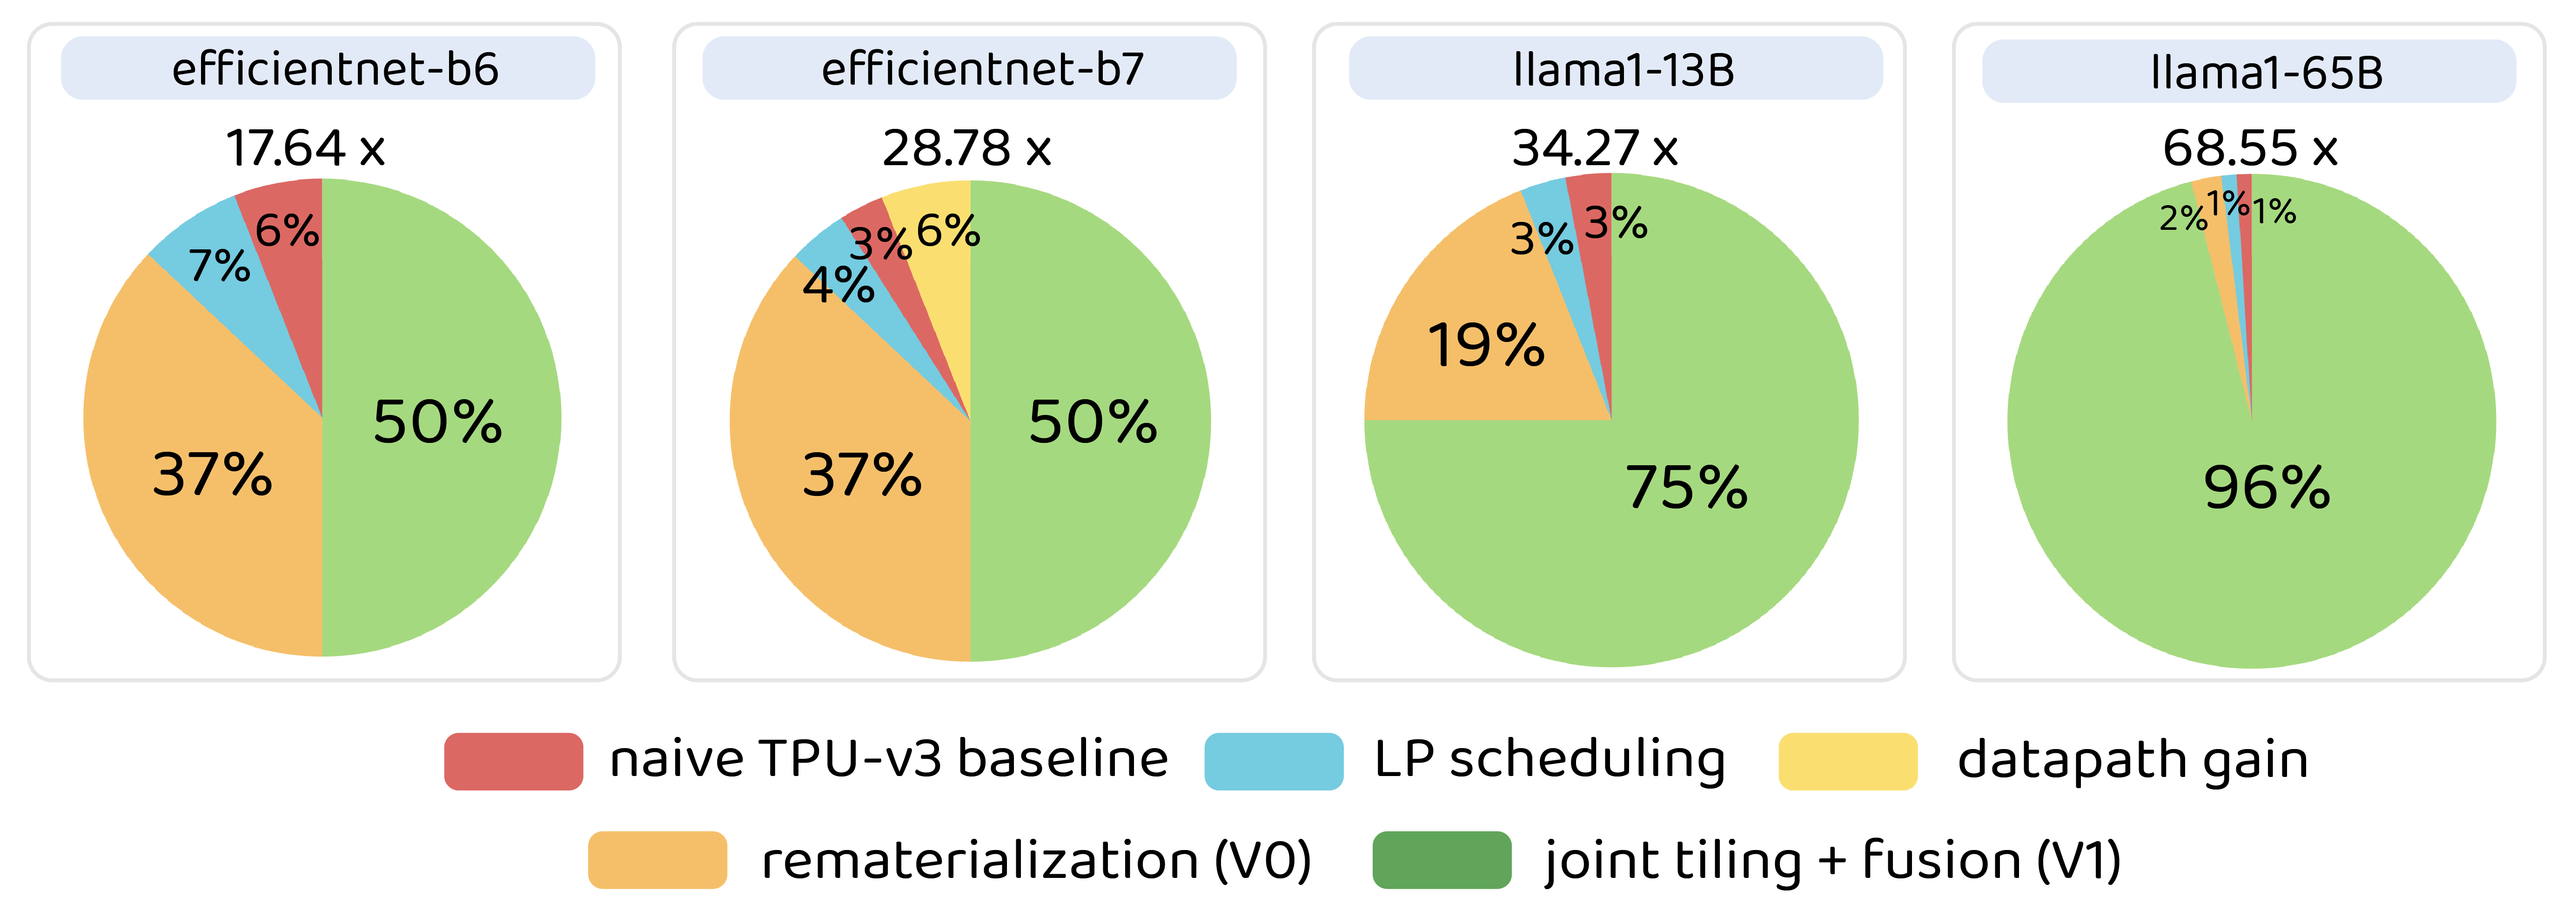
\includegraphics[width=0.85\linewidth]{fig3/speedup_decomposition_final_v2.png}
% \caption{Speedup decomposition over naive TPU-v3 baseline. Each pie shows the 
% relative contribution of four optimization sources to the total speedup. CHEETAH-V1 joint tiling + fusion dominates on all workloads, 
% especially on larger models where memory management is the primary bottleneck.}\label{fig:accel_decompose}
% \end{figure}
% \subsubsection{Static Baseline vs.\ CHEETAH-V0 vs.\ CHEETAH-V1 Unlock Progressive Gains}


% Figure~\ref{fig:accel_decompose} decomposes the total speedup over a naive TPU-v3 baseline into four sources: LP-based scheduling and fusion, datapath gain from hardware search, dynamic rematerialization (CHEETAH-V0), and joint tiling + fusion (CHEETAH-V1).

% The dominant contributor across all workloads is V1's joint tiling-fusion 
% optimization. On EfficientNet-B1, V1 accounts for 50\% of total speedup, 
% with LP scheduling (28\%) and datapath gain (22\%) splitting the remainder---and 
% no rematerialization benefit, consistent with B1's small activation footprint 
% fitting comfortably in Global Memory. B3--B4 show a similar 50\% V1 share, but 
% V0 rematerialization now contributes 25\%, reflecting the growing value of 
% recomputing large depthwise activations rather than reloading them from DRAM. 
% From B5 onward, V1's share rises sharply to 75--88\%, as the increasing 
% model size makes joint tiling-fusion the primary lever: memory management 
% dominates, and the remaining sources (LP scheduling, V0, datapath) each shrink 
% to single-digit percentages. The same pattern holds on Llama, where V1 accounts 
% for 83--87\% of the total speedup.

% % \begin{wrapfigure}{r}{0.48\textwidth}
% %     \centering
% %     \vspace{-12pt}
% %     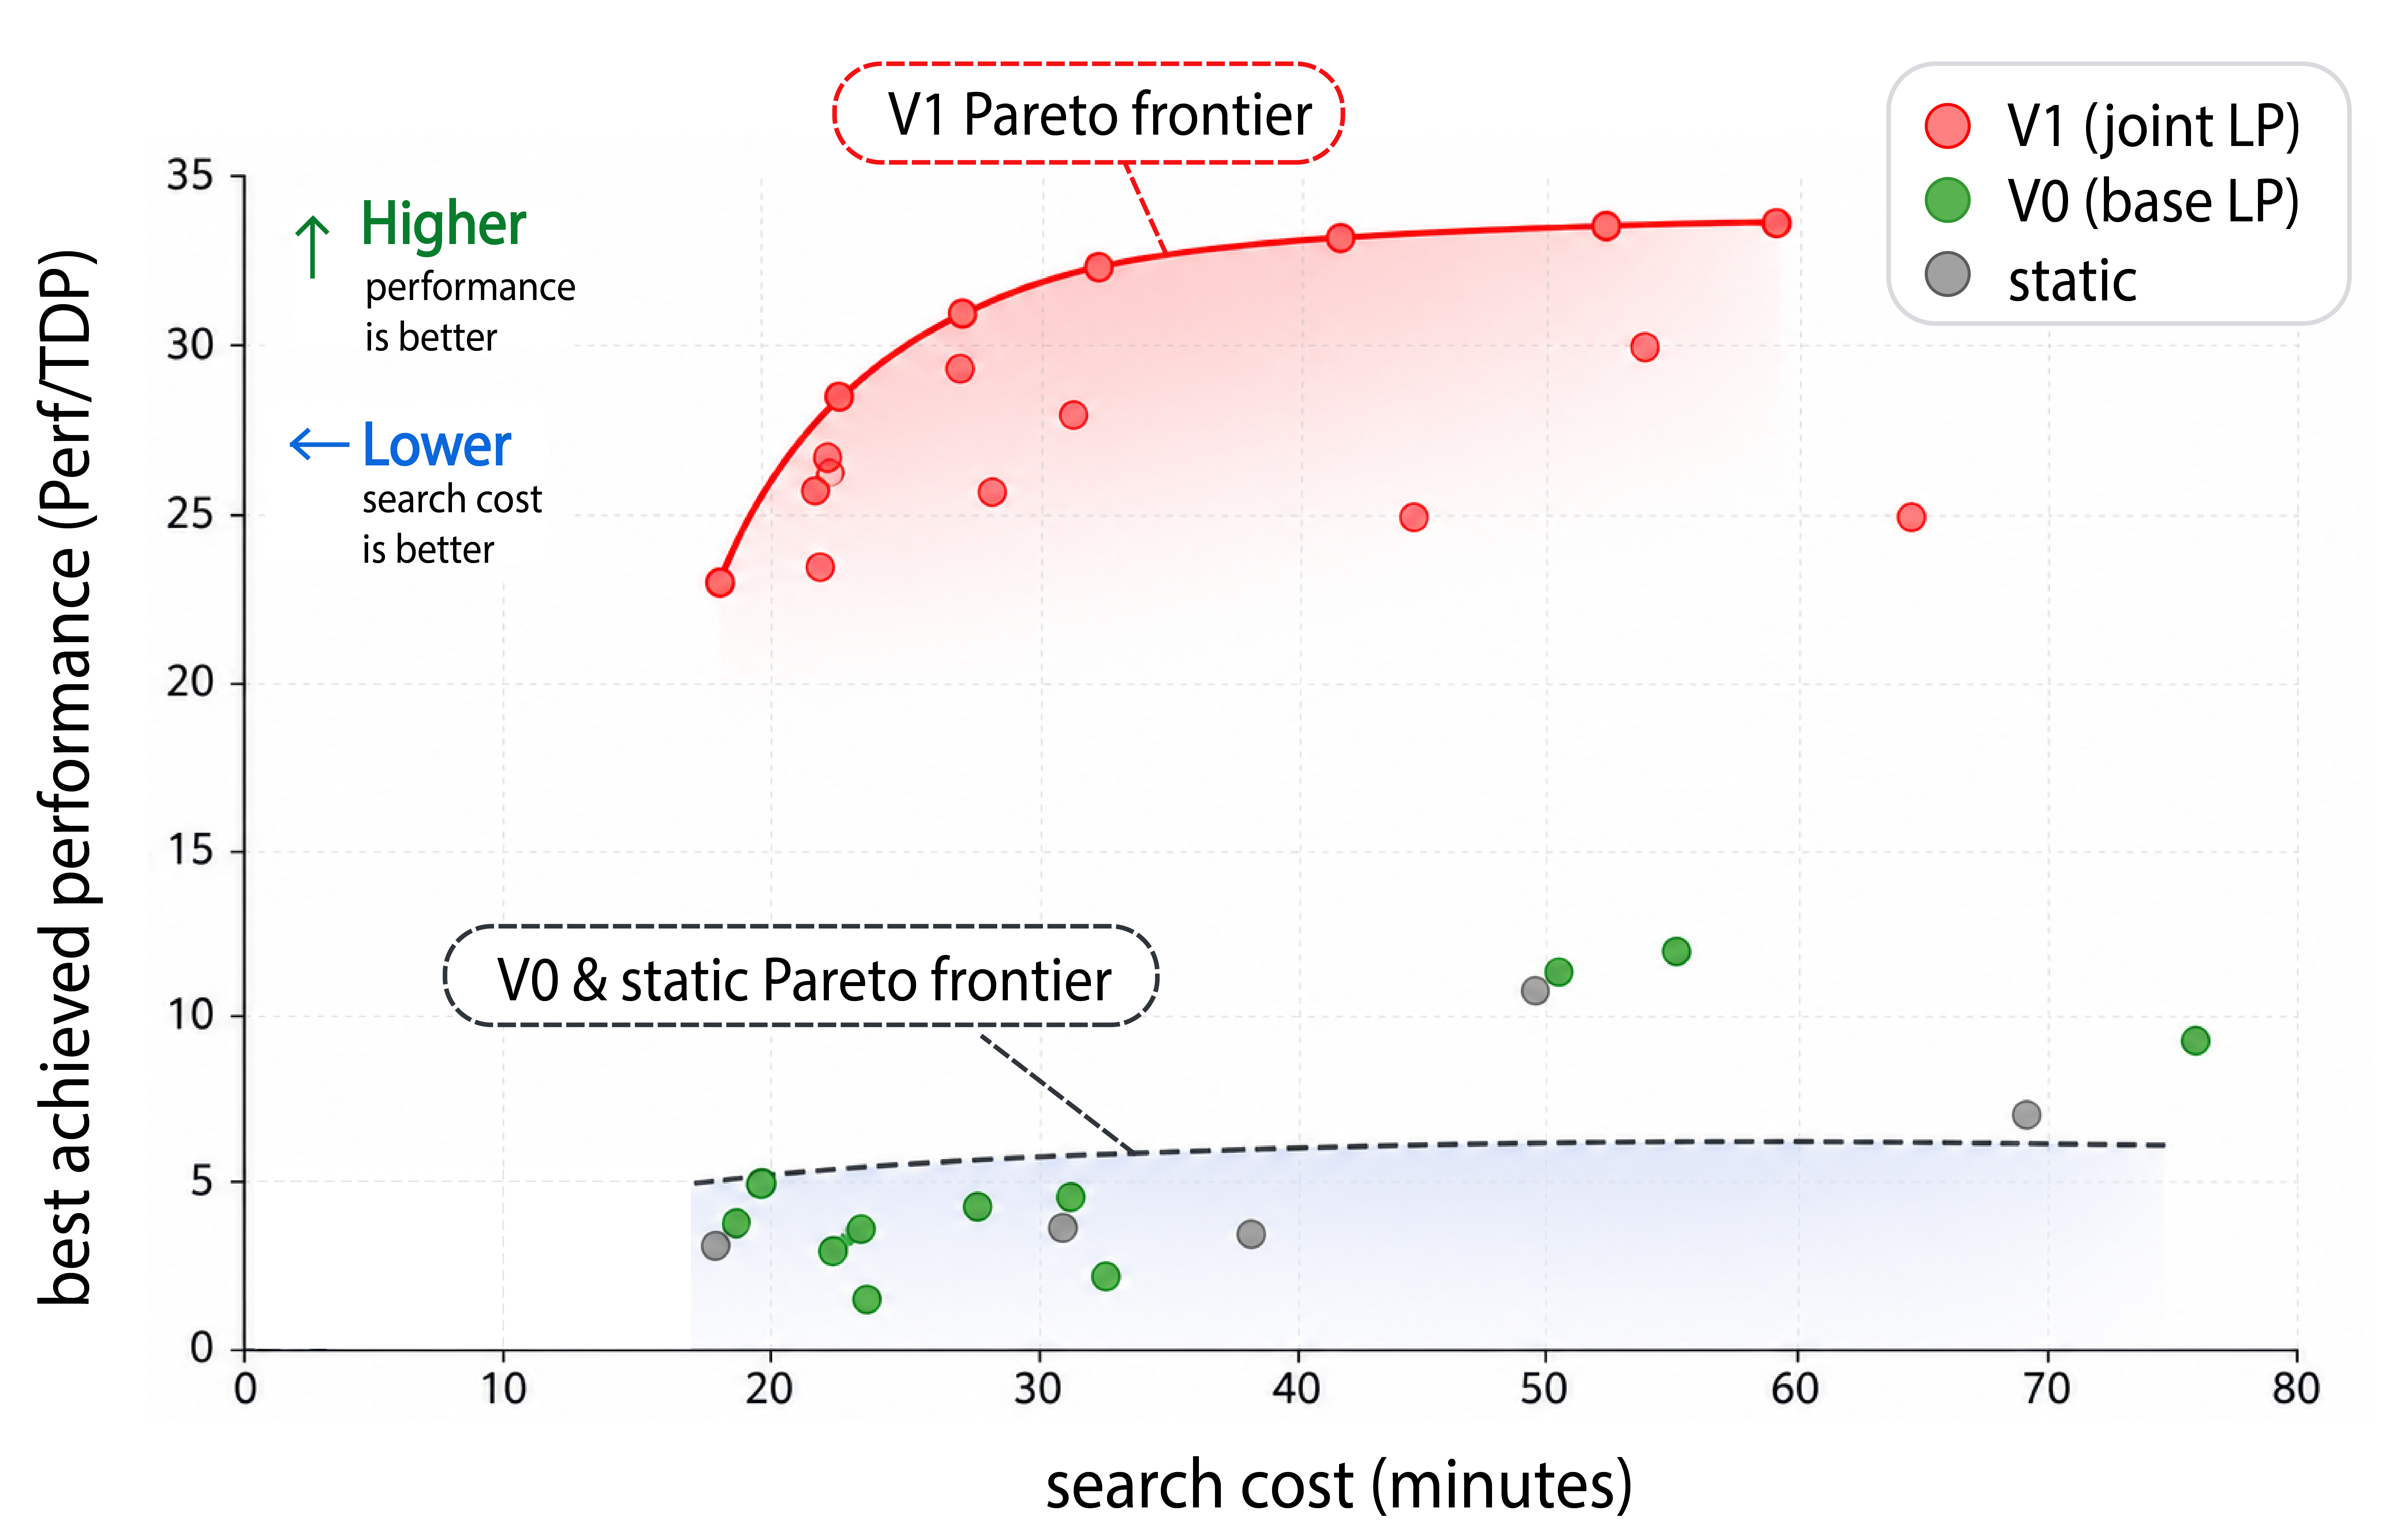
\includegraphics[width=0.48\textwidth]{figs/pareto_v2.png}
% %     \vspace{-18pt}
% %     \caption{Search cost vs.\ Perf/TDP Pareto frontier. V1 dominates V0 and static across all time budgets.}
% %     \label{fig:pareto}
% %     \vspace{-10pt}
% % \end{wrapfigure}

% Critically, Figure~\ref{fig:speedup} shows static fusion method is \emph{infeasible} on modern large models (Llama-70B, and DeepSeek-V3), because their large activation tensors cannot fit under a static pinning policy. The V0 formulation resolves feasibility for on large models via dynamic placement but remains time-intensive for a small number of 50 trials: measuring 58.42 hours on Llama-70B and 69.39 hours on DeepSeek-V3 (Figure~\ref{fig:wallclock}). In contrast Figures~\ref{fig:wallclock} and ~\ref{fig:speedup}, show the CHEETAH-V1 formulation out performs comparitive strategies in terms of speedup against the TPU-V3 baseline, and require only 1.17 hours on Llama-70B and 2.17 hours on DeepSeekv3 for 50 trails---a ${\sim}93\%$ average reduction. The powerful joint formulation is able to select memory-efficient tiling configurations alongside placement, achieving feasibility across the entire workload suite, demonstrating that joint optimization is not merely an incremental improvement but a qualitative capability unlock for large-scale models.

% % This demonstrates that by exploiting structural invariance and GPU-accelerated mathematical optimization, CHEETAH-V1 reduces the end-to-end co-design search time from days to under 2.2 hours—a ${\sim}93\%$ average reduction—while discovering architectural points that deliver up to $35\times$ speedup over the TPU-v3 baseline.

% % Figure~\ref{fig:pareto} shows the Pareto frontier of best-achieved Perf/TDP versus wall-clock search cost. V1 strictly dominates both V0 and static at every time budget: within 10 minutes of search, V1 already exceeds the best Perf/TDP that V0 or static achieve after 60+ minutes. The V1 Pareto frontier reaches ${\sim}35\times$ Perf/TDP, roughly $3\times$ higher than the V0/static frontier at ${\sim}10\text{--}12\times$. This gap reflects two compounding advantages: V1 explores a strictly larger feasible region (joint tiling-fusion), and it eliminates Timeloop from the per-trial critical path, allowing more trials within any fixed time budget.



% \paragraph{Practical insight.}
% Both LPs are extreme-aspect-ratio sparse: for \texttt{llama3\_70b},
% $m, n \sim 10^6$ and $\mathrm{nnz} \sim 5 \times 10^6$, giving roughly
% 1 nonzero per million matrix entries.
% The time-band structure means a coordinate-descent or stochastic PDHG
% solver would converge in $\mathcal{O}(T)$ sweeps if bands were the only
% structure.
% The capacity rows in both V0 and V1 LP formulations are the sole feature breaking strict banded structure, and they are precisely what couples the schedule globally. This is the desired behavior of a memory-aware placement formulation.

% % \todo{Report LP solve times for V0 and V1 across all benchmarks. Compare wall-clock time per trial against FAST's SCIP-based ILP solver (20 min timeout). Report LP relaxation gap: how often do fractional solutions need integer rounding, and what is the quality loss from rounding?}

% \paragraph{Structural invariance.}
% For a fixed workload and LP formulation, the LP constraint matrix
% has an invariant sparsity pattern across trials: the row/column
% dimensions and nonzero locations are determined only by the model graph structure — layer count $L$, timestep count $T$, edge set $E$, and Pareto count $C$ — not by the hardware candidate.
% Vizier changes only numerical values such as cycle coefficients,
% memory-capacity bounds, bandwidth-scaled access costs, objective weights, and TDP/area parameters. 
% This invariance allows us to reuse the same sparse matrix structure,
% variable ordering, block layout, and JIT-compiled sparse kernels in our adapted JAX PDLP solver across all hardware trials for a given workload.

% Numerically, we apply the same diagonal preconditioning pipeline
% on each trial: a structural presolve with 20 log-geomean Ruiz iterations, followed by the PDLP preprocessing stack with 10 infinity-norm Ruiz iterations and one Pock--Chambolle $\ell_1$-scaling pass. This two-stage diagonal scaling handles the mixed coefficient magnitudes present in V0/V1 matrices — large byte-valued capacity rows together with $\pm 1$ persistence rows — without requiring a fragile matrix factorization.

% In production, this preconditioning pipeline is reused structurally across trials, recomputes only cheap diagonal scalings, finishes in under one second for matrices with approximately $5 \times 10^6$ nonzeros, and avoids factorization failures entirely because it consists only of $D_1 A D_2$ arithmetic.

% \subsubsection{LLM Architect vs. Optimizer}
% The LLM Architect framework is modeled on SkyDiscover, and efficiently prunes the large outer hardware search loop by proposing campaign patches. Rather than predicting performance, the Architect reads a compact Causal Ledger containing invalid-rate history, MFU, roofline lower-bound checks, and LP diagnostics, then proposes a constrained hardware neighborhood for Vizier to search locally. The V1 LP remains the sole performance evaluator: for each candidate, it solves the joint tiling, fusion, placement, and rematerialization LP, while a deterministic Roofline Auditor rejects physically impossible results. In the widened V1 search space, all methods reach the same capped V1 Perf/TDP ceiling, so the key differentiator is search efficiency. The LLM loop reduces invalid hardware evaluations from 24.5\% under full-space Vizier to 5.9\% on average across five workloads, a 4.1× reduction in wasted trials, while preserving the same best V1 score. This shows that the LLM’s contribution is not replacing Vizier or the solver, but steering Bayesian optimization toward feasible, workload-appropriate architectural neighborhoods with far less wasted trials. This also sets the foundation for future work, where the LLM in the loop can adhere to follow more complex human reasoning signals.
% \begin{figure}[ht!]
%     \centering
% 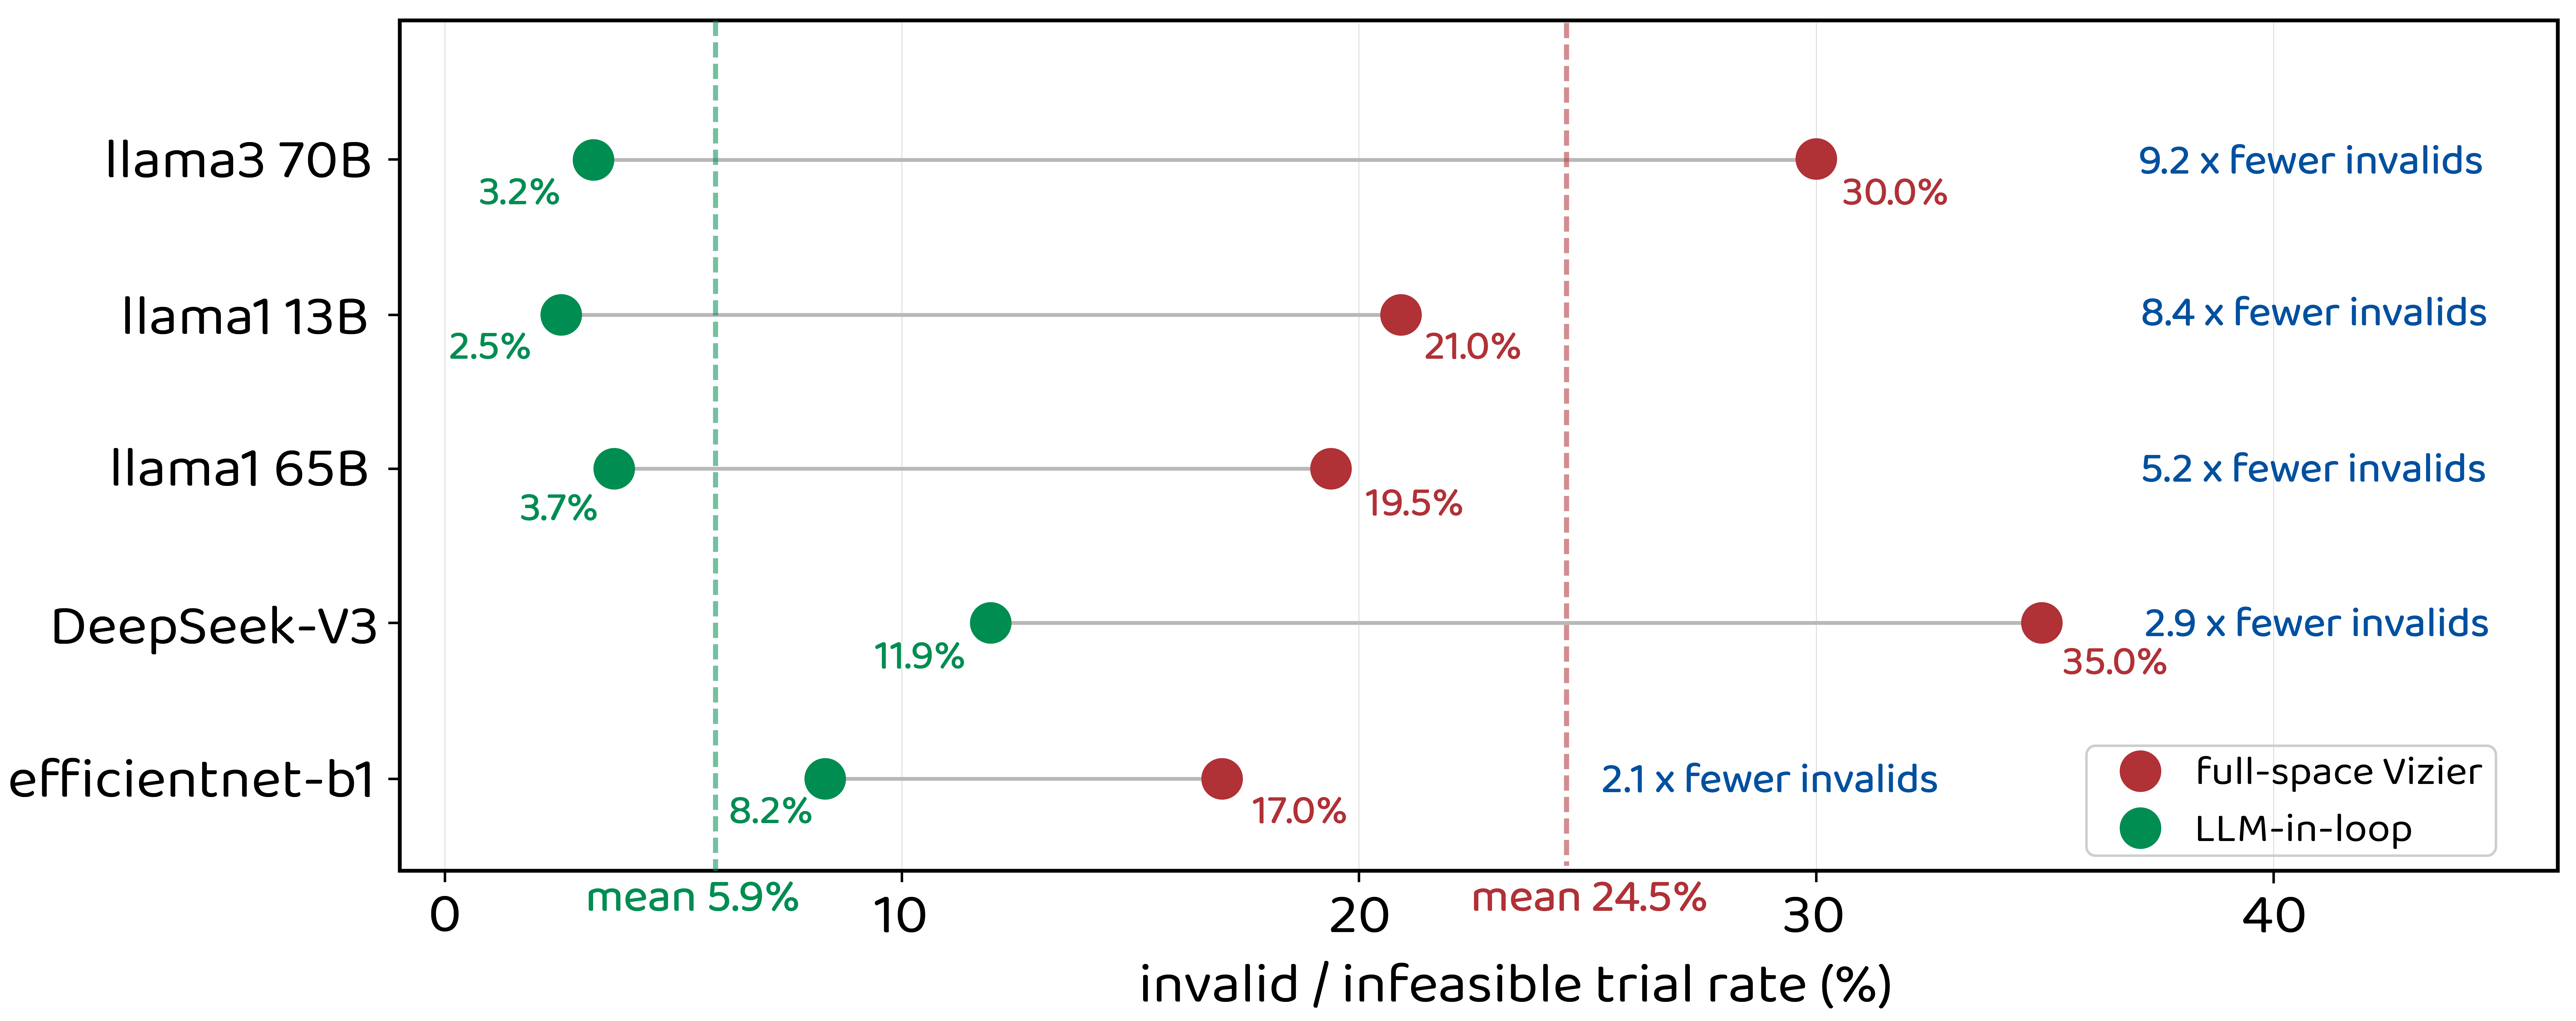
\includegraphics[width=0.85\linewidth]{fig3/llm_guide_v1.png}
% \caption{Strategic Intelligence vs. Stochastic Brute Force}\label{fig:llm}
% \end{figure}



% % The LLM should not just ask, “What chip has the best Perf/TDP?” We aim to answer the question “Given this user’s workload and deployment goal, what is the architectural region to search for this deployment task?”. Therefore we have the LLM emit profile-conditioned campaigns that take specific user inference tasks into consideration. For each $(\text{deployment profile},\ \text{workload})$ cell, we ran a
% % 200-trial LLM-Architect experiment using the same Qwen2.5-7B-Instruct + LoRA with differing user input profiles. At the start of each round, the prompt was assembled from a fixed system
% % prompt, the active deployment profile, three few-shot examples, and a per-round user message containing the workload, recent feedback signals, current search bounds, and the causal ledger.
% % The Strategist returned a one-line JSON campaign patch, which the
% % validator accepted only if it was a strict legal subset of the parent space, satisfied hard rules such as patch-volume $\leq 10\%$, ridgepoint and MAC/BW constraints, and avoided forbidden regions.

% % Thus, the experiment isolates whether the profile-conditioned LLM prompt alone can steer the same V1 evaluator toward different hardware families under different deployment intents.



% % \todo{Compare convergence rate of LLM-guided hardware search vs.\ Vizier-only (Bayesian, LCS, random baselines) in the style of FAST Figure~11. Report:
% % \begin{itemize}
% %     \item Number of trials to reach $X\%$ of best Perf/TDP found by 5,000-trial Vizier
% %     \item Quality of LLM-proposed configurations vs.\ Vizier-proposed configurations
% %     \item Qualitative analysis of LLM reasoning about hardware bottlenecks
% % \end{itemize}
% % }

% % \subsubsection{ROI Analysis}

% % \todo{Update FAST's ROI analysis (Table~4) with the improved Perf/TDP numbers from FAST-CORGI. Report deployment volumes required to reach 1$\times$, 2$\times$, 4$\times$ ROI targets. If Perf/TDP improvements are larger than FAST's, the break-even deployment volume should decrease correspondingly.}

% % \subsubsection{Pareto Frontier}

% % \todo{Plot the Perf/TDP vs.\ area Pareto frontier for V1-optimized designs compared to FAST and TPU-v3 baseline, analogous to FAST Figure~12.}


% edit for page limit
% \vspace{-0.3cm}
\section{Experiments}
\label{sec:experiments}
Experiments span full CHEETAH V0 and V1 pipelines and the LLM Architect across $12$ workloads: $11$ vision and language models plus the Stable Diffusion~1.5 UNet. We benchmark against TPU-v3 because it is the production deep learning accelerator with the most publicly documented microarchitecture, process, and power figures~\citep{jouppi2017datacenter,jouppi2021ten}, which lets every comparison be normalized to a disclosed chip and stay consistent with prior work~\citep{zhang_fast}. For the fixed-hardware study we add a second, deliberately generic hardware point, a compact edge NPU (Section~\ref{sec:fixed_hw}), so that the scheduling gains are shown on both ends of the provisioning spectrum.
~\cref{sec:exp_intro} introduces our experimental setting, sanity checks, and physical manufacturability validation gates.
~\cref{sec:prog} examines progressive unlocked speedup gains between LP formulations,~\cref{sec:breakdown} provides the breakdown of accelerator performance,
~\cref{app:custom_solve} summarizes our custom systems solver design, and~\cref{app:blueprint_tables} provides discussion on CHEETAH custom accelerator blueprint analysis.
% \vspace{-0.2cm}




\subsection{Experimental Setup}
\label{sec:exp_intro}
% \vspace{-0.2cm}
We benchmark against the static FAST framework~\citep{zhang_fast} using a simulated TPU-v3 \citep{jouppi2021ten} baseline normalized to sub-10nm process technology (within $8.2 \pm 2.7\%$ of profiled TPU-v3 performance). We use a custom adapted JAX PDLP solver for large models (Llama-70B, DeepSeek-V3) and HiGHS \citep{huangfu2018parallel} for smaller models, reporting speedup over the TPU-v3 baseline in order to be consistent with prior work.
We evaluate across 12 workloads: EfficientNet-B1 \citep{tan2019efficientnet} through B7 (stressing low-intensity depthwise convolutions), Llama-1 13B/65B and Llama-3 70B \citep{llama3modelcard}, DeepSeek-V3-MoE \citep{deepseekv3report} (stressing memory capacity and bandwidth), and the Stable Diffusion~1.5 UNet, a $346$-operation diffusion backbone with long skip connections (stressing bandwidth-bound activation traffic). Each workload is optimized independently under 100 trials per method. For Static and V0 methods, the pipeline is Vizier$\to$Timeloop$\to$LP; for the V1 method, the pipeline simplifies to Vizier$\to$LP. 
The LLM Architect outer loop proposes search-space interventions for Vizier using Lagrangian dual feedback, and is only permitted to change Vizier's search neighborhood while the strict LP inner loop remains unchanged.

\paragraph{Physical Design Validation.} Since modeling simulations ultimately present a gap with real world physical performance, we validate all results through a five-level audit process: (i) Roofline Auditor, (ii) Campaign Validator, (iii) Causal Ledger, (iv) solver diagnostics, and (v) six pre-RTL gates. Each CHEETAH design must pass all five audit tiers before it is deemed feasible and reported. 

The roofline auditor confirms the basic and necessary condition that the reported LP latency is not physically impossible: no result is faster than either the compute or memory lower bound. All reported CHEETAH results are roofline-feasible with zero lower-bound violations. 
The pre-RTL manufacturability gates aim to ensure that CHEETAH-designed chips can fit a single TSMC N7 reticle, has a wirable pin-out for four HBM3 stacks, meets $1\,\mathrm{GHz}$ timing, has a wirable NoC, fits an AIO cooler envelope, and decomposes into standard SRAM macros.
This seeks to close the gap between simulation at research-level, and a physical design chip that could plausibly be taped out.
\cref{tab:mfg_gates} summarizes the six gate definitions, with detailed numerical reports and discussion provided in Appendix~\ref{app:details}. 


\begin{table}[t]
\centering
\small
\caption{Manufacturability gate definitions. Each candidate hardware configuration must pass all six gates before being accepted as a feasible design, rather than a theoretical Pareto-frontier point that exists only in LP space. These are not post-hoc screens applied to a finished design: every one of them is a row of the program itself, so the optimizer cannot return a design that violates them. The pin-count limit, for instance, enters as a linear constraint on bandwidth, which removes the illegal bandwidth branches from the menu before any design is scored. A gate can therefore only be reported as satisfied, never as repaired.}
\label{tab:mfg_gates}
\begin{tabularx}{\linewidth}{lXr}
\toprule
\textbf{Gate} & \textbf{What it checks} & \textbf{Threshold} \\
\midrule
1.\ Pin count    &
  HBM3-class signal pins at $0.8$\,GB/s/pin &
  $\le 4{,}096$ pins \\[0.3em]
2.\ Reticle area &
  Linear area model on 7\,nm &
  $\le 600$\,mm$^2$ \\[0.3em]
3.\ Logic depth  &
  MAC-tree combinational depth &
  $\le 35$ levels \\[0.3em]
4.\ NoC routing  &
  $n_{\mathrm{PEs}} \times n_{\mathrm{banks}}$ cells &
  $\le 5\times10^6$ \\[0.3em]
5.\ Power density &
  $P_{\mathrm{dyn}} / A_{\mathrm{die}}$ &
  $\le 2.0$\,W/mm$^2$ \\[0.3em]
6.\ SRAM macros  &
  64\,KiB banks; aspect ratio $\in [1{:}4,\, 4{:}1]$ &
  $\le 4{,}096$ banks \\
\bottomrule
\end{tabularx}
\end{table}



% \subsection{Main Results}

% \subsubsection{V0 vs.\ FAST Static Fusion}

% \todo{Insert results table and figure comparing V0 (time-indexed placement + rematerialization) against FAST's static fusion ILP on all benchmarks. Key metrics: Perf/TDP improvement, fusion efficiency (\% of DRAM stall time eliminated), rematerialization frequency (how often does the solver choose to recompute rather than reload?).}

% \paragraph{Expected findings.}
% V0's dynamic placement should show the largest gains on workloads with: (1)~tight Global Memory budgets where static pinning wastes capacity on tensors that are only needed briefly, (2)~long dependency chains where tensor lifetimes vary substantially, and (3)~cheap-to-recompute operations with large activations (\eg, depthwise convolutions in EfficientNet).

% \subsubsection{V1 vs.\ V0: Joint Tiling and Fusion}

% \todo{Insert results table and figure comparing V1 against V0 on all benchmarks. Key metrics: Perf/TDP improvement, number of operations where V1 selects a different tiling configuration than Timeloop's greedy choice, and the resulting compute efficiency vs.\ fusion trade-off.}

% \paragraph{Expected findings.}
% V1 should show the largest gains on architectures with highly diverse layer types where a single tiling configuration cannot serve all operations well. EfficientNet (depthwise + pointwise convolutions with 100$\times$ variation in working-set sizes) and hybrid CNN-transformer models (convolutions + attention + MLP with fundamentally different compute-memory profiles) are expected to benefit most.


% \subsubsection{stiatic vs v0 vs v1}
% \begin{figure}[ht!]
%     \centering
%     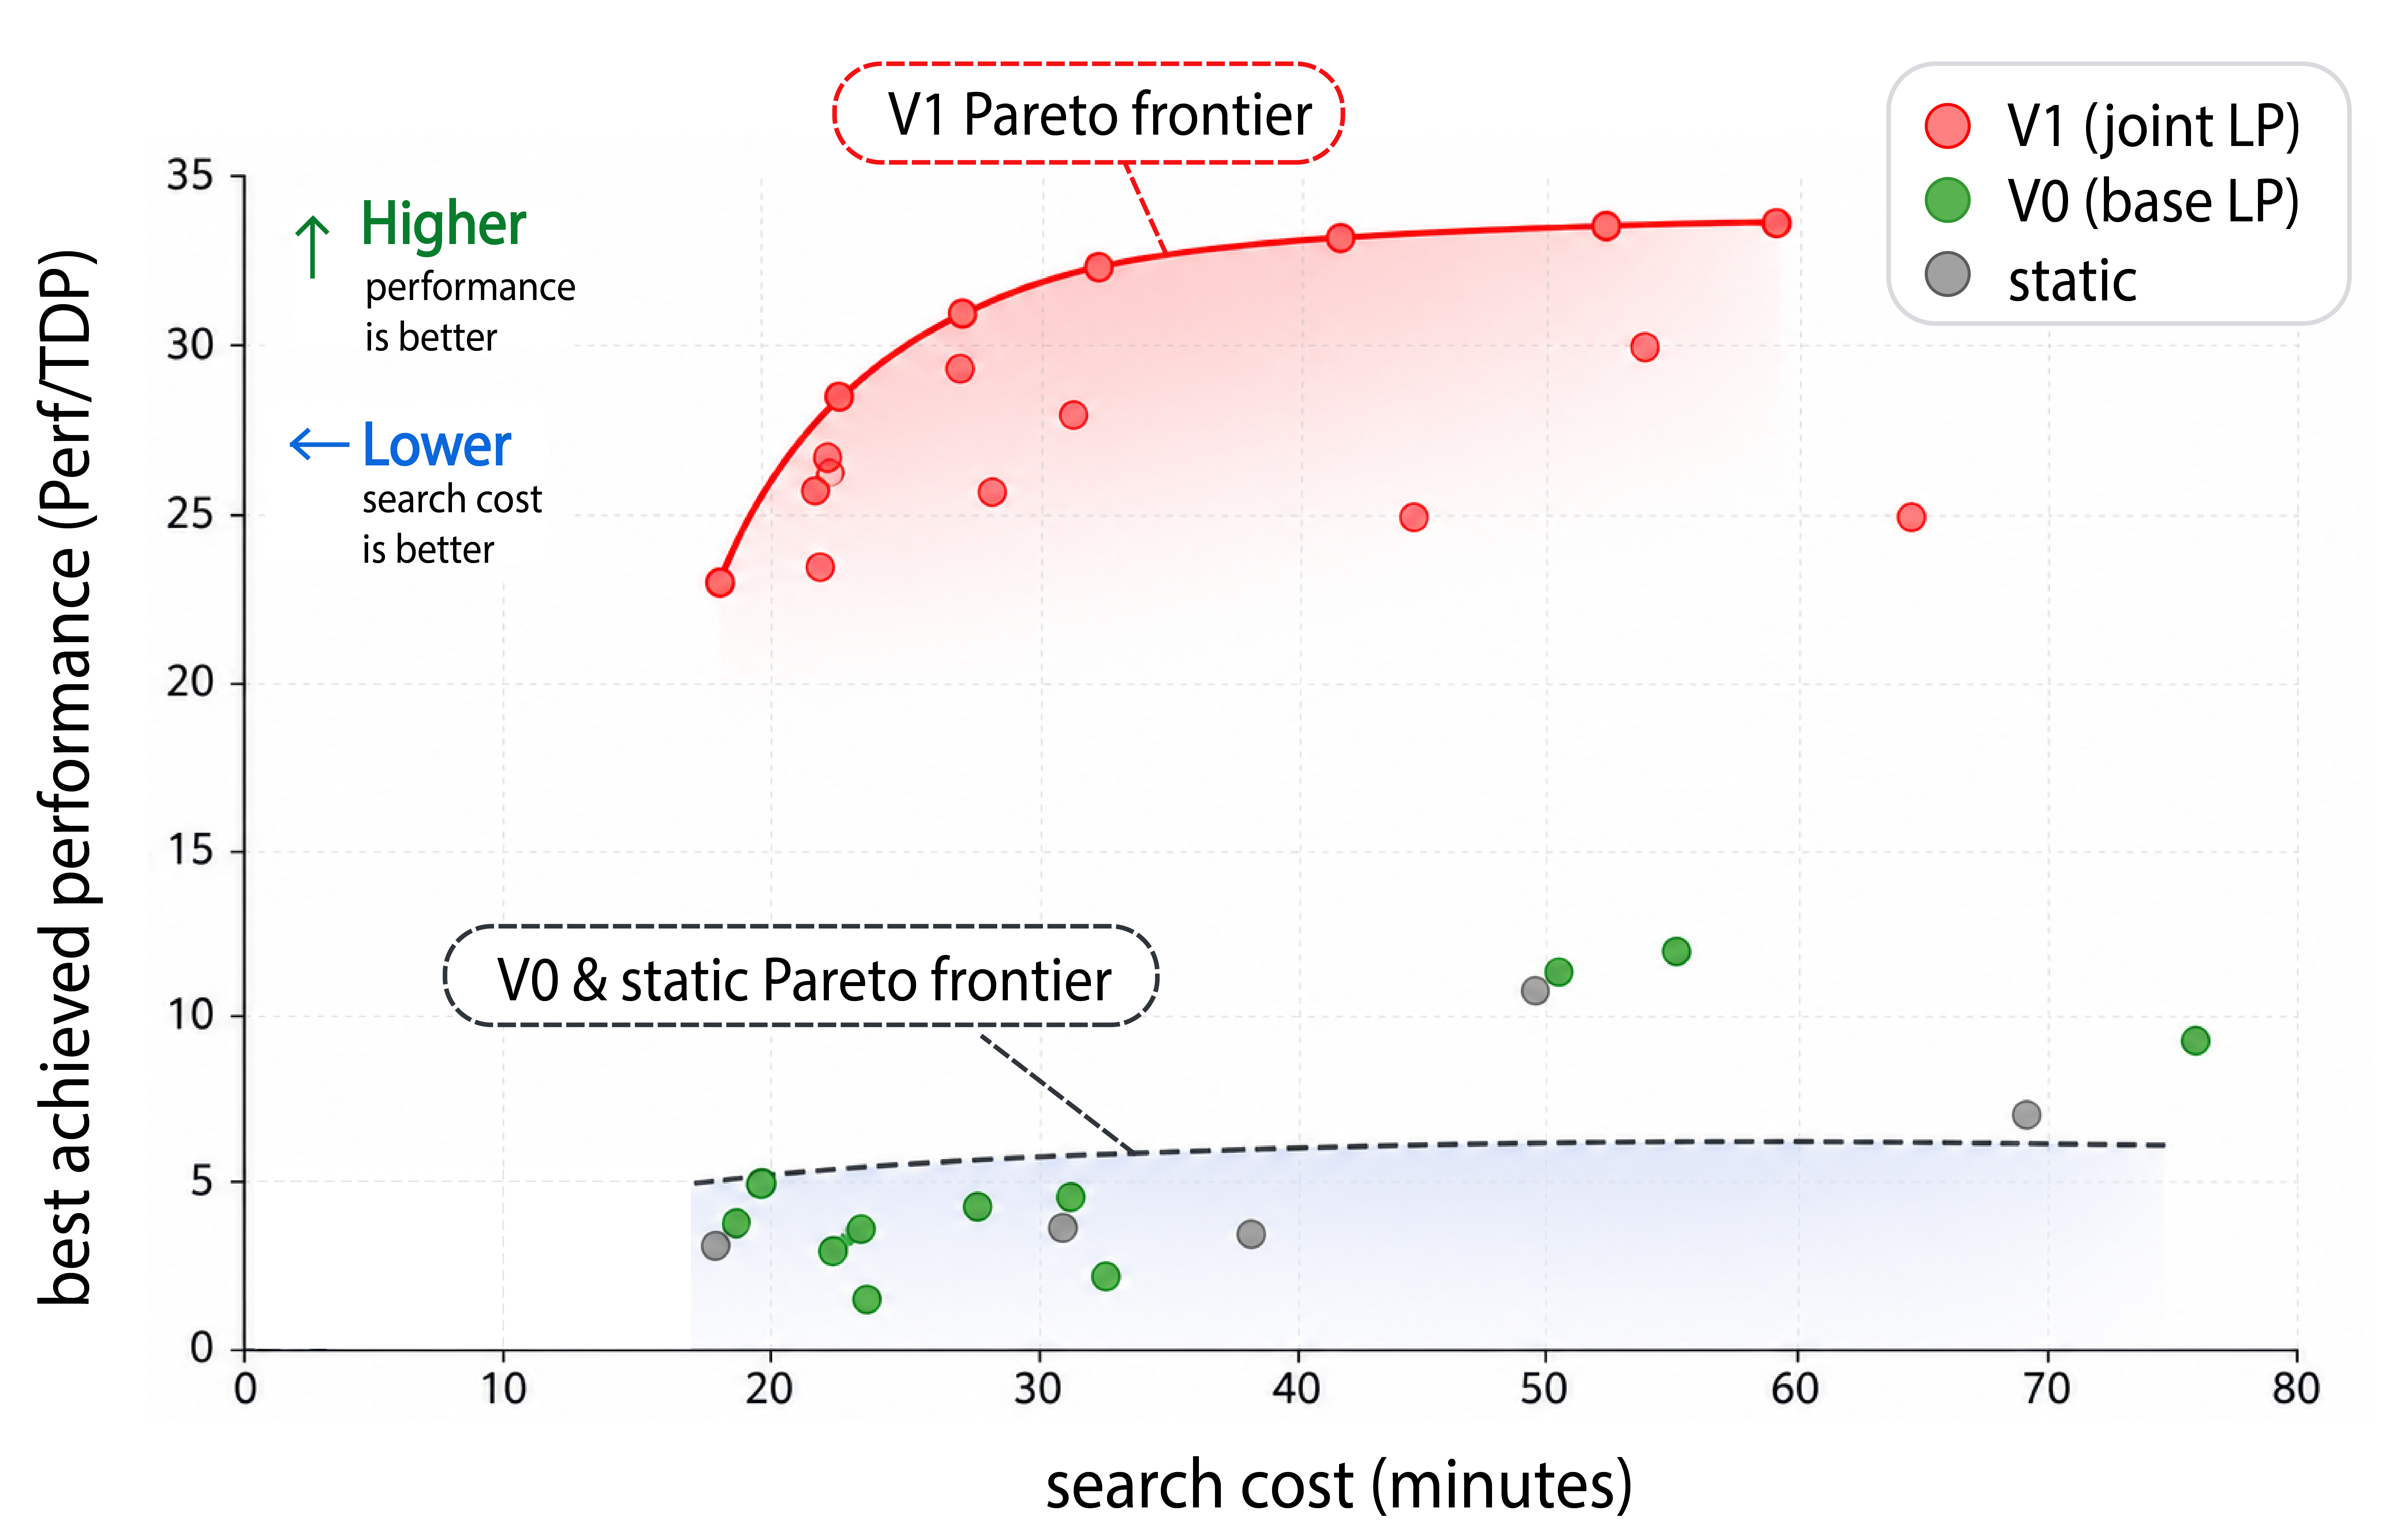
\includegraphics[width=0.7\linewidth]{figs/pareto_v2.png}
%     \caption{pareto frontier plot}
% \end{figure}
\begin{figure}[ht!]
    \centering
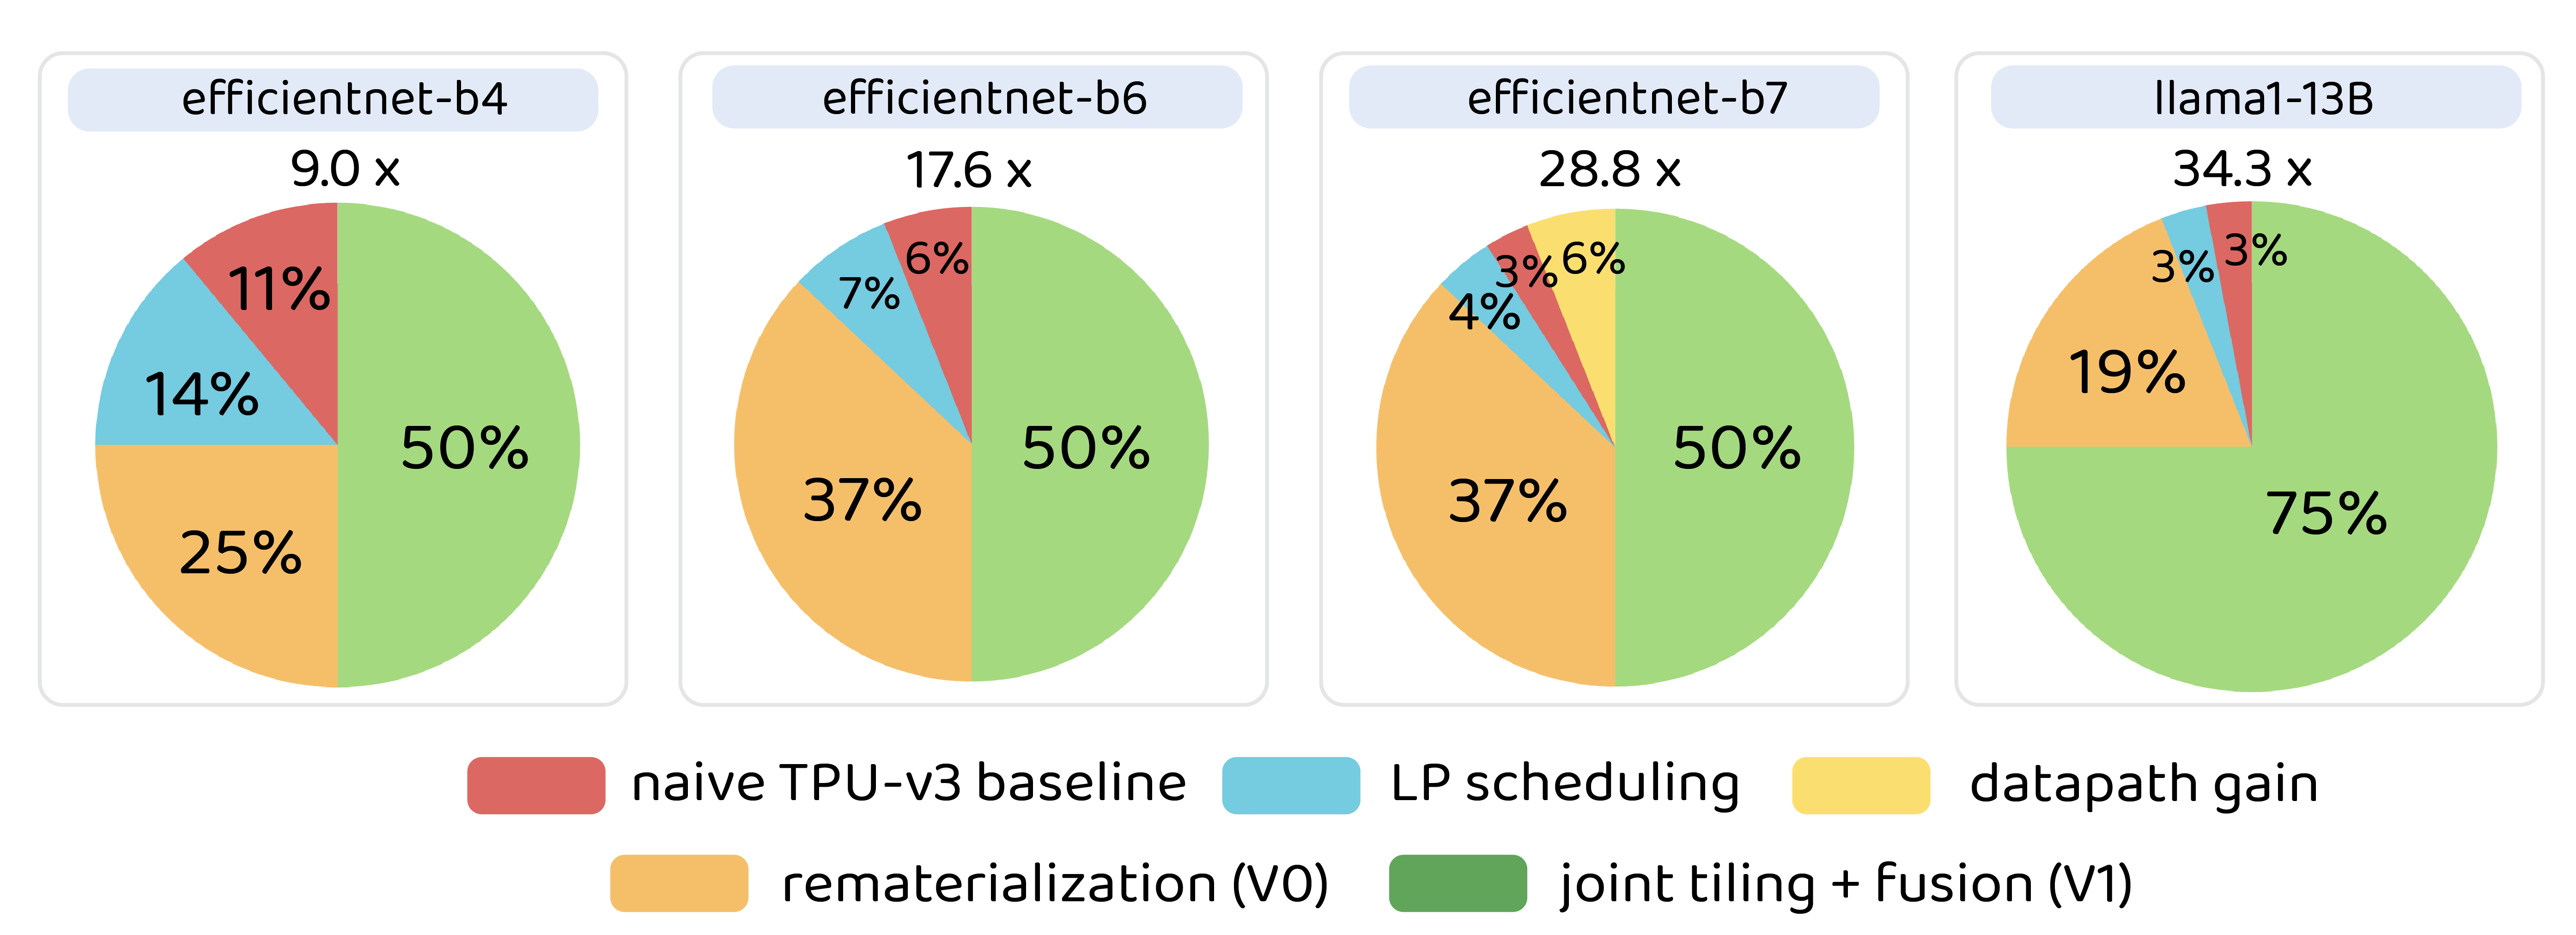
\includegraphics[width=0.85\linewidth]{fig3/speedup_decomposition_final_v4.png}
\caption{Speedup decomposition over naive TPU-v3 baseline. Each pie shows the 
relative contribution of four optimization sources to the total speedup. CHEETAH-V1 joint tiling + fusion dominates on all workloads, 
especially on larger models where memory management is the primary bottleneck.}\label{fig:accel_decompose}
\end{figure}
\subsection{Static Baseline vs.\ CHEETAH-V0 vs.\ CHEETAH-V1 Unlock Progressive Gains}
\label{sec:prog}

Figure~\ref{fig:accel_decompose} decomposes the total speedup over a naive TPU-v3 baseline into four sources: LP-based scheduling and fusion, datapath gain from hardware search, dynamic rematerialization (CHEETAH-V0), and joint tiling + fusion (CHEETAH-V1). Table~\ref{tab:LP_struct} in \cref{append::lp_perform} gives side-by-side structural comparison of the V0 and V1 formulation matrices in greater detail. 

The dominant contributor across all workloads is V1's joint tiling-fusion 
optimization. V1's share grows with model size: from 50\% on B1--B4 to 75--88\% from B5 onward and 83--87\% on Llama, reflecting that memory management increasingly dominates as models scale. On smaller models, LP scheduling and datapath gains split the remainder; V0 rematerialization contributes ${\sim}25\%$ on B3--B4 where recomputing large depthwise activations outperforms DRAM reloads.

Critically, Figure~\ref{fig:speedup} shows the static fusion method is \emph{infeasible} on modern large models (Llama-70B, and DeepSeek-V3), because their large activation tensors cannot fit under a static pinning policy. The V0 formulation resolves feasibility on large models via dynamic placement, while V1 further improves by jointly selecting memory-efficient tiling configurations alongside placement, achieving feasibility across the entire workload suite. This demonstrates that joint optimization is not merely an incremental improvement but a qualitative capability unlock for large-scale models. Additional optimization details and observations are provided in Appendix~\ref{app:details}. We further provide two interesting examples of optimal tiling solutions the V1 formulation proposed in Appendix~\ref{app:tiling}.

\begin{figure}[ht!] 
    \centering
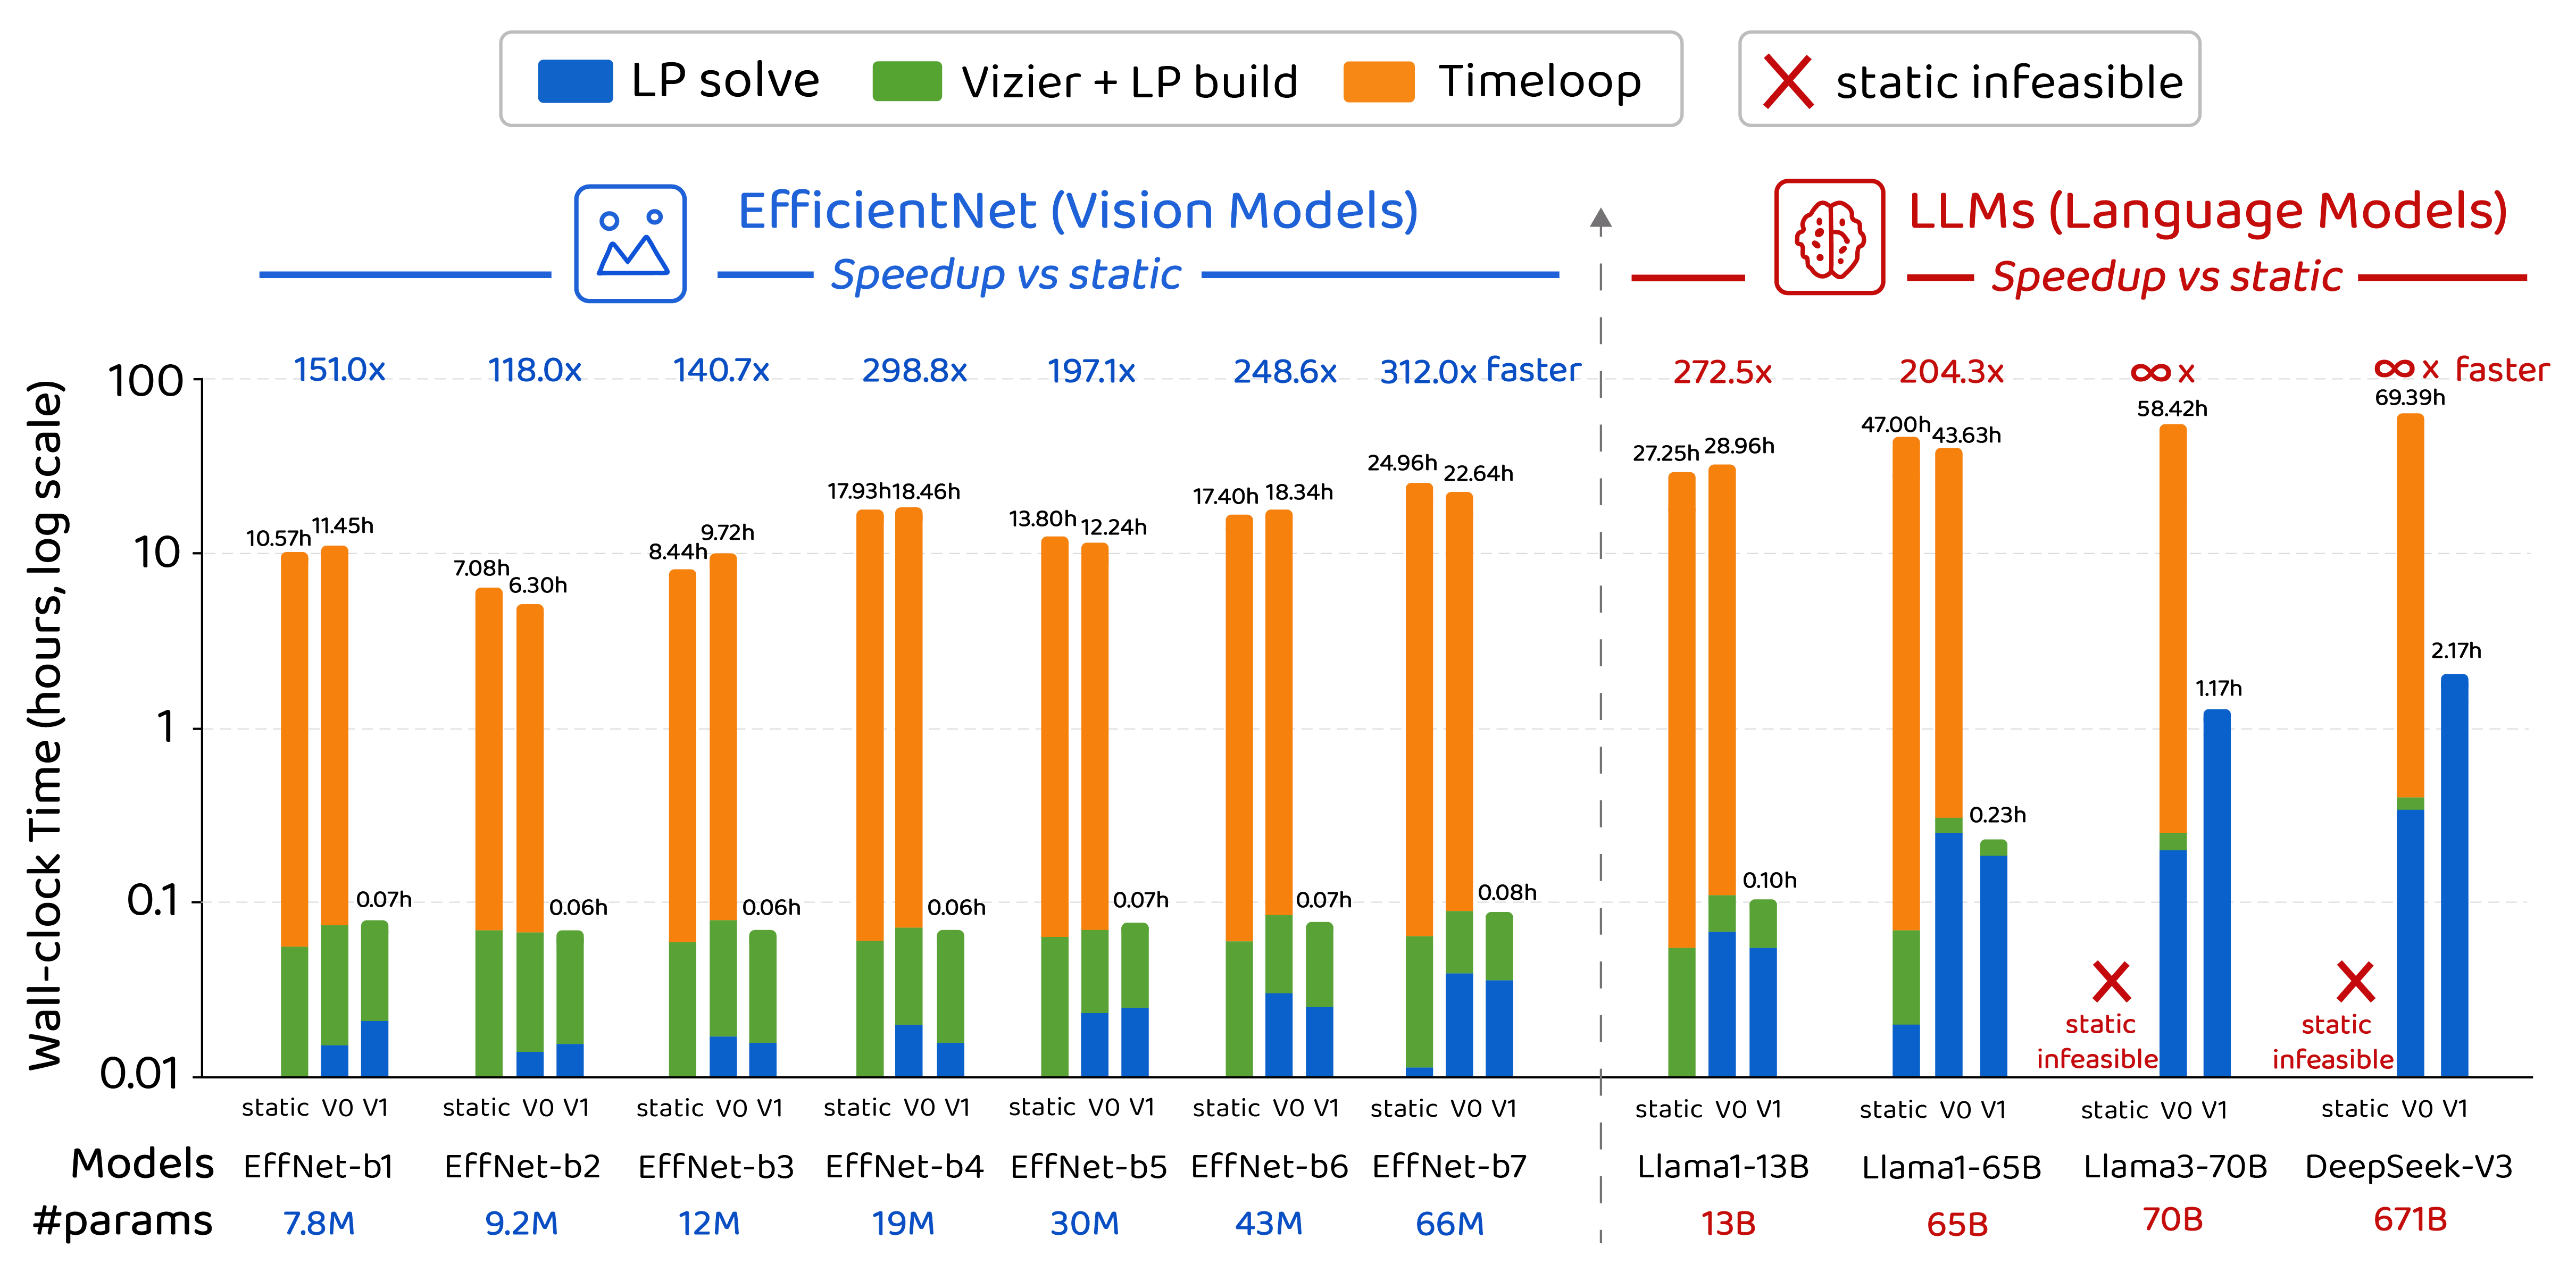
\includegraphics[width=1.0\linewidth]{fig3/wallclock_new_v6.png}
\caption{Wall-clock time decomposition and performance acceleration across formulations: CHEETAH-V1's internalized tiling eliminates the Timeloop bottleneck, achieving up to 100--300$\times$ faster search than the classical static method. Upper bars show wall-clock hours (log scale); annotations show speedup vs.\ static.}
\label{fig:wallclock}
\end{figure}

\subsection{Same-Silicon Fixed-Hardware Speedup}
\label{sec:fixed_hw}
The speedup decomposition of Figure~\ref{fig:accel_decompose} folds hardware search into the reported gains. To isolate CHEETAH's scheduling contribution from silicon provisioning, we hold the chip \emph{fixed} and compare the joint CHEETAH-V1 schedule against a naive streaming schedule on the \emph{same} silicon. Because the identical chip appears in both the numerator and the denominator of every ratio, these speedups are equal-area and equal-TDP by construction and require no resource normalization. We evaluate two fixed-hardware baselines: the simulated TPU-v3 (900\,GB/s, 32\,MiB on-chip) and a compact edge NPU representative of Jetson-Orin-Nano-class parts ($32{,}768$ INT8 MACs at $1$\,GHz, ${\sim}65$\,TOPS, $64$\,GB/s LPDDR5, $16$\,MiB on-chip). We additionally include Stable Diffusion~1.5 UNet (SD1.5-UNet), a $346$-operation diffusion UNet with long skip connections, to stress a bandwidth-bound regime distinct from the CNN and LLM suites.

\begin{table}[t]
\centering
\caption{Same-silicon fixed-hardware speedup: the joint CHEETAH-V1 schedule vs.\ a naive streaming schedule on the \emph{identical} chip. Speedup is $T_{\text{naive}}/T_{\text{joint}}$ under the same cost-model convention on that chip's own per-layer cache (naive $=\sum T_{\max}$ streaming); MFU is model-MFU (cache compute-floor over latency within one convention), not measured silicon utilization. Ratios are equal-area/TDP by construction. Bold marks the best speedup per chip.}
\label{tab:fixed_hw}
\scriptsize
\setlength{\tabcolsep}{4.5pt}
\renewcommand{\arraystretch}{1.22}
\definecolor{bandtpu}{RGB}{230,239,253}
\definecolor{bandnpu}{RGB}{230,245,233}
\definecolor{rowalt}{gray}{0.955}
\definecolor{rowgeo}{gray}{0.875}
\begin{tabular}{@{}l ccc ccc@{}}
\toprule
 & \multicolumn{3}{c}{\cellcolor{bandtpu}\textbf{TPU-v3} (900\,GB/s, 32\,MiB)}
 & \multicolumn{3}{c}{\cellcolor{bandnpu}\textbf{Compact NPU} (64\,GB/s, 16\,MiB)} \\
\cmidrule(lr){2-4}\cmidrule(lr){5-7}
\textbf{Workload} & MFU$_{\text{naive}}$ & MFU$_{\text{joint}}$ & Speedup & MFU$_{\text{naive}}$ & MFU$_{\text{joint}}$ & Speedup \\
\midrule
Llama-1 13B     & 0.467 & 1.000 & $2.14\times$ & 0.022 & 0.694 & $\mathbf{31.4\times}$ \\
\rowcolor{rowalt}
Llama-3 70B     & 0.399 & 1.000 & $\mathbf{2.51\times}$ & 0.043 & 0.330 & $7.66\times$ \\
DeepSeek-V3     & 0.451 & 1.000 & $2.22\times$ & 0.043 & 0.330 & $7.8\times$ \\
\rowcolor{rowalt}
SD1.5-UNet      & 0.643 & 0.963 & $1.50\times$ & 0.038 & 0.223 & $5.89\times$ \\
\midrule
\rowcolor{rowgeo}
\textbf{Geomean} & & & $\mathbf{2.06\times}$ & & & $\mathbf{10.3\times}$ \\
\bottomrule
\end{tabular}
\end{table}

Table~\ref{tab:fixed_hw} reports $T_{\text{naive}}/T_{\text{joint}}$ per cell, where the naive denominator is a $\sum T_{\max}$ streaming schedule computed under the same cost-model convention on each chip's own per-layer cache. On the TPU-v3 the joint schedule delivers $1.50$--$2.51\times$ (geomean $2.06\times$); on the compact NPU the gains are markedly larger, $5.89$--$31.4\times$ (geomean $10.3\times$). This gap is a direct consequence of bandwidth: at $64$\,GB/s the naive streaming schedule is severely memory-starved, running at a model-MFU of only $0.02$--$0.04$, so the placement and residency structure of the joint LP recovers a far larger fraction of idle time. SD1.5-UNet exemplifies this sensitivity: its $1.50\times$ TPU-v3 gain rises to $5.89\times$ on the edge NPU, tracking the same inverse-bandwidth trend as the LLMs because the diffusion UNet is bandwidth-bound once on-chip capacity is tight. All model-MFU values are the cache compute-floor divided by LP latency within a single convention, not measured silicon utilization: on the TPU-v3 the joint schedule recovers model-MFU from a naive $0.40$--$0.64$ to $0.96$--$1.00$ (a near-pure utilization recovery, not additional compute), while on the bandwidth-starved edge NPU the joint model-MFU ($0.22$--$0.69$) is the physical roofline, honestly below one.

\subsection{Wall-Clock Acceleration and LLM Outer Loop Search Efficiency}
\label{sec:breakdown}
Figure~\ref{fig:wallclock} reveals a striking practical advantage of V1: by internalizing tiling into the LP, it removes Timeloop from the per-trial critical path, collapsing each trial to a single Vizier-proposal and LP-solve step. On EfficientNet models, V1 completes 50 trials 151--312$\times$ faster than the static pipeline. On LLMs the acceleration is even more dramatic: V0 requires 58.42 hours on Llama-70B and 69.39 hours on DeepSeek-V3 for 50 trials, whereas V1 requires only 1.17 hours and 2.17 hours respectively, a ${\sim}93\%$ average reduction. This speedup arises because Timeloop accounts for over 99\% of per-trial latency in the sequential pipeline (Figure~\ref{fig:timeloop-time}), and V1 eliminates this bottleneck entirely via precomputed Pareto tiling sets that are reused across all Vizier trials sharing the same compute configuration class. The combination of higher speedup \emph{and} dramatically lower search cost makes V1 strictly dominant: it explores a larger feasible design space in a fraction of the wall-clock time. 

% \begin{wrapfigure}{r}{0.48\textwidth}
% \vspace{-12pt}
% \centering
% 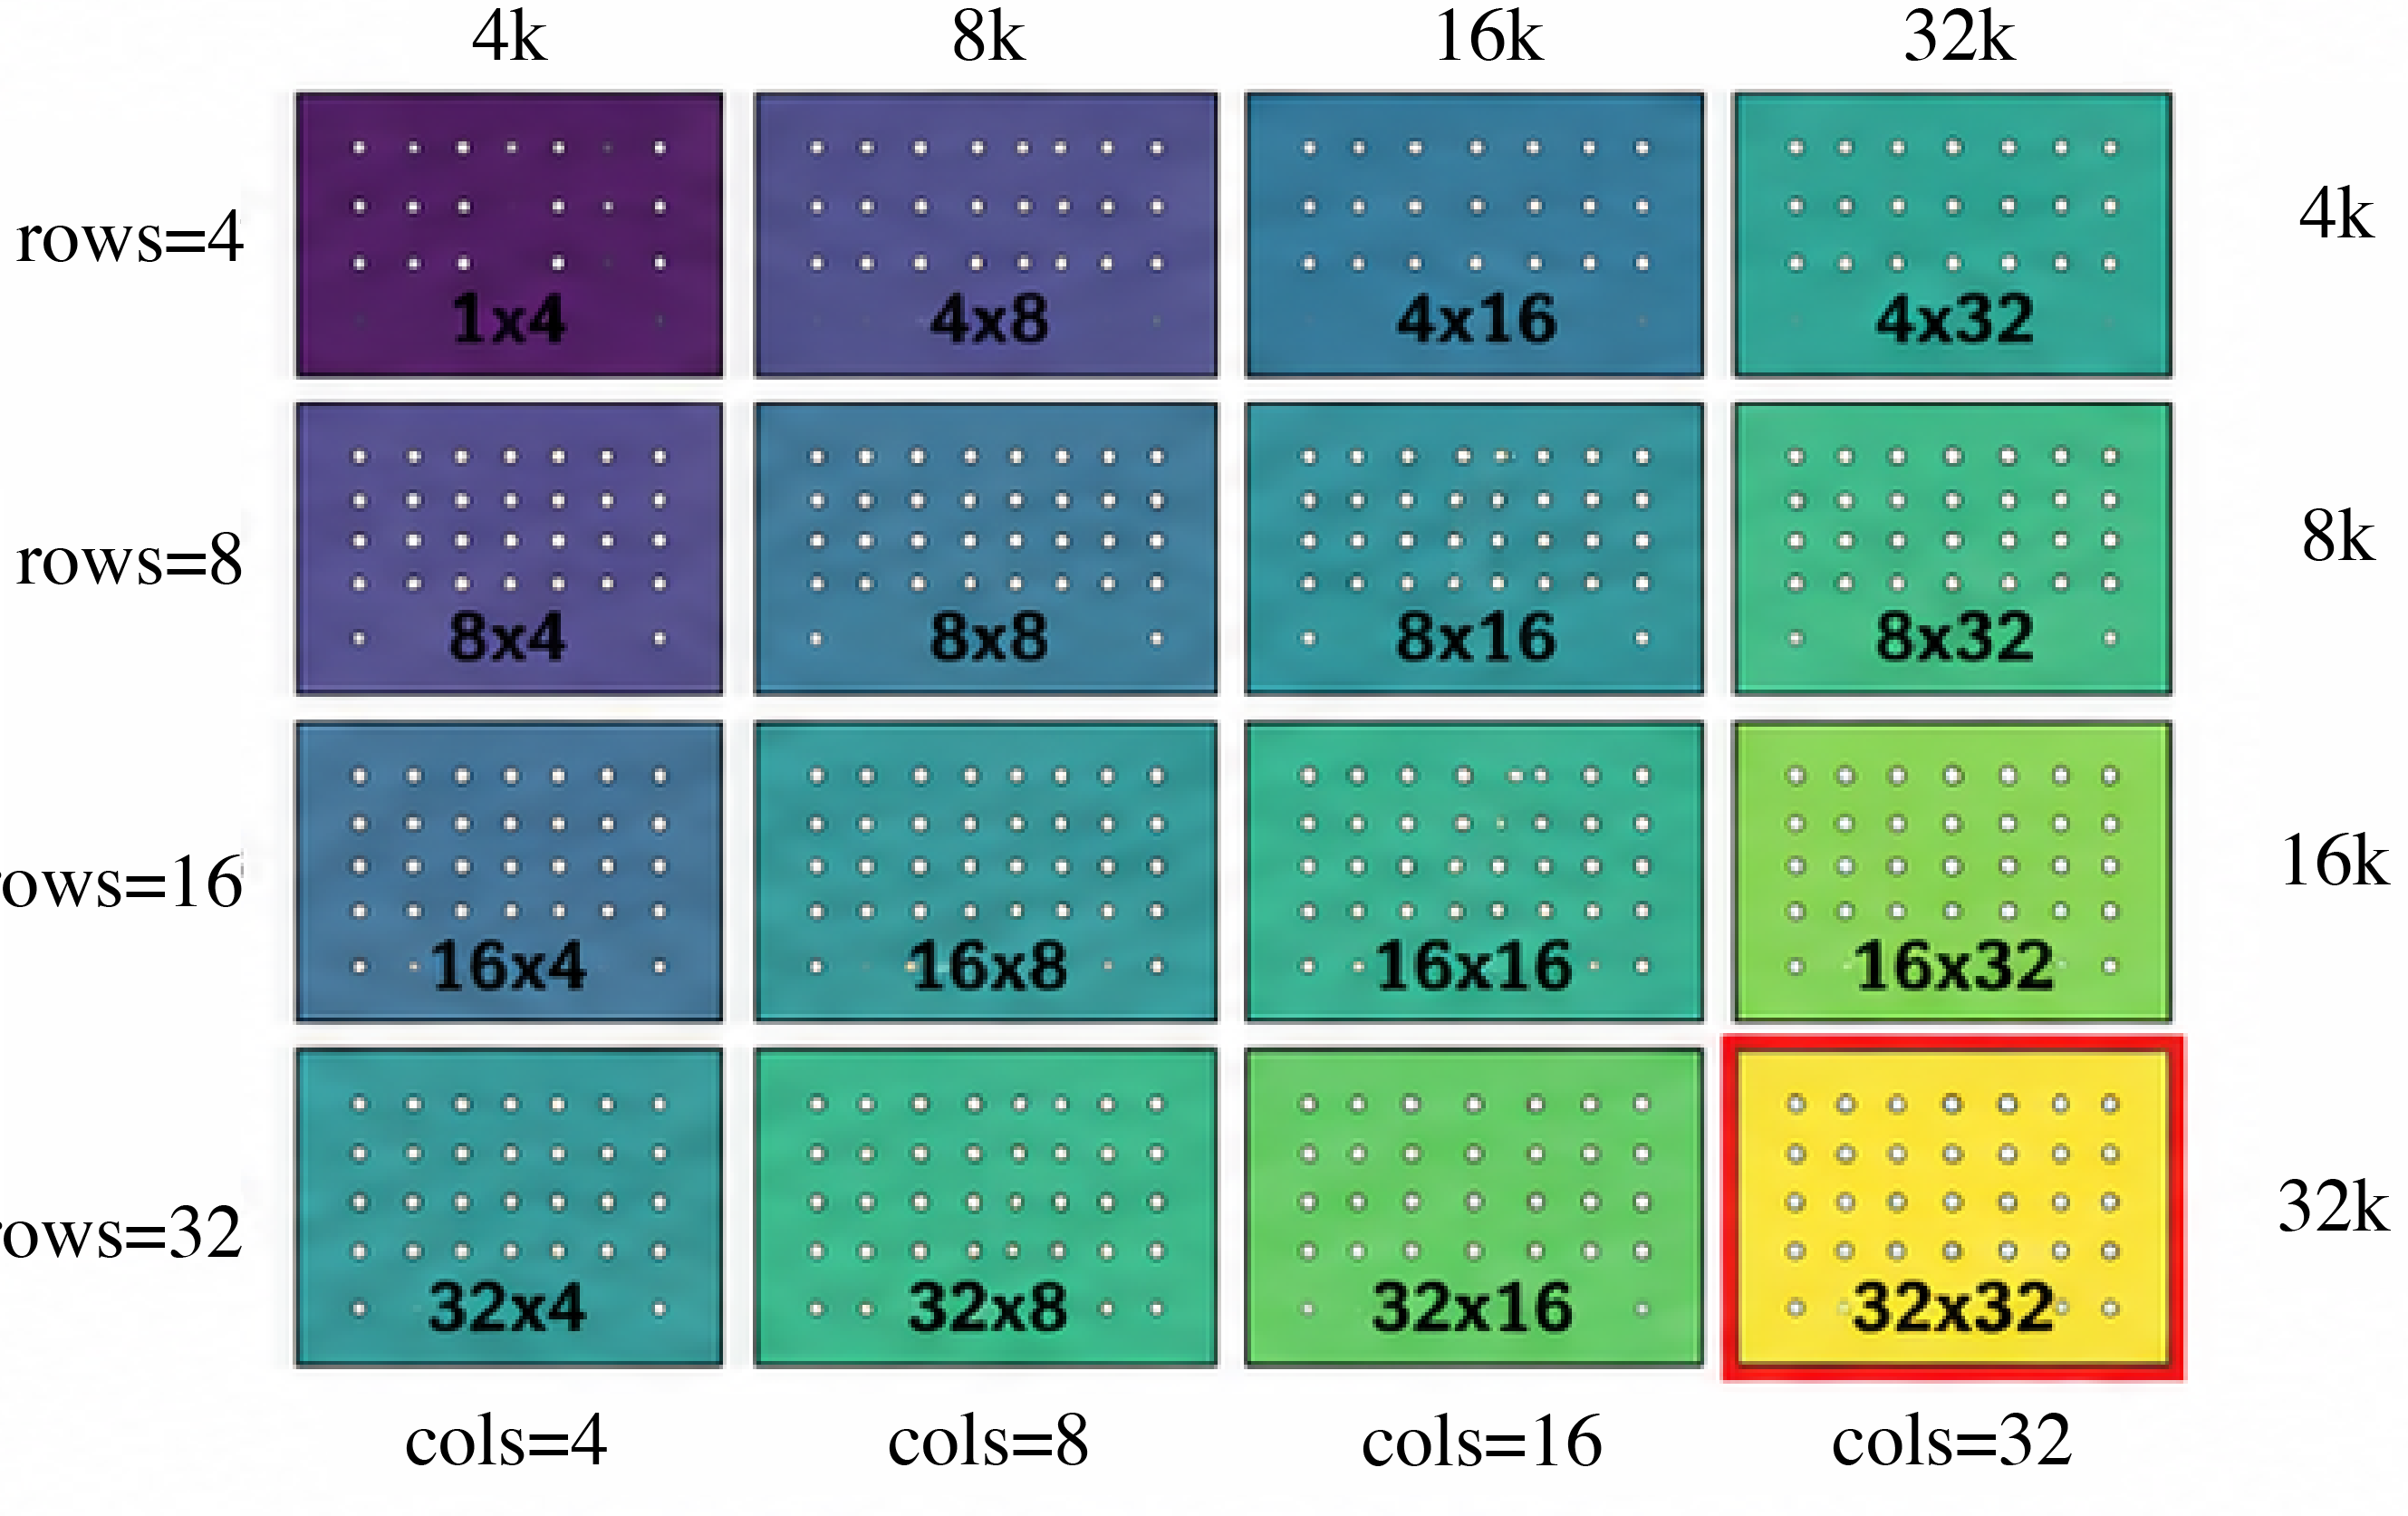
\includegraphics[width=0.46\textwidth]{figs4/tiles.png}
% \caption{Caption here.}
% \label{fig:tiles}
% \vspace{-14pt}
% \end{wrapfigure}
\begin{figure}[h]
\centering
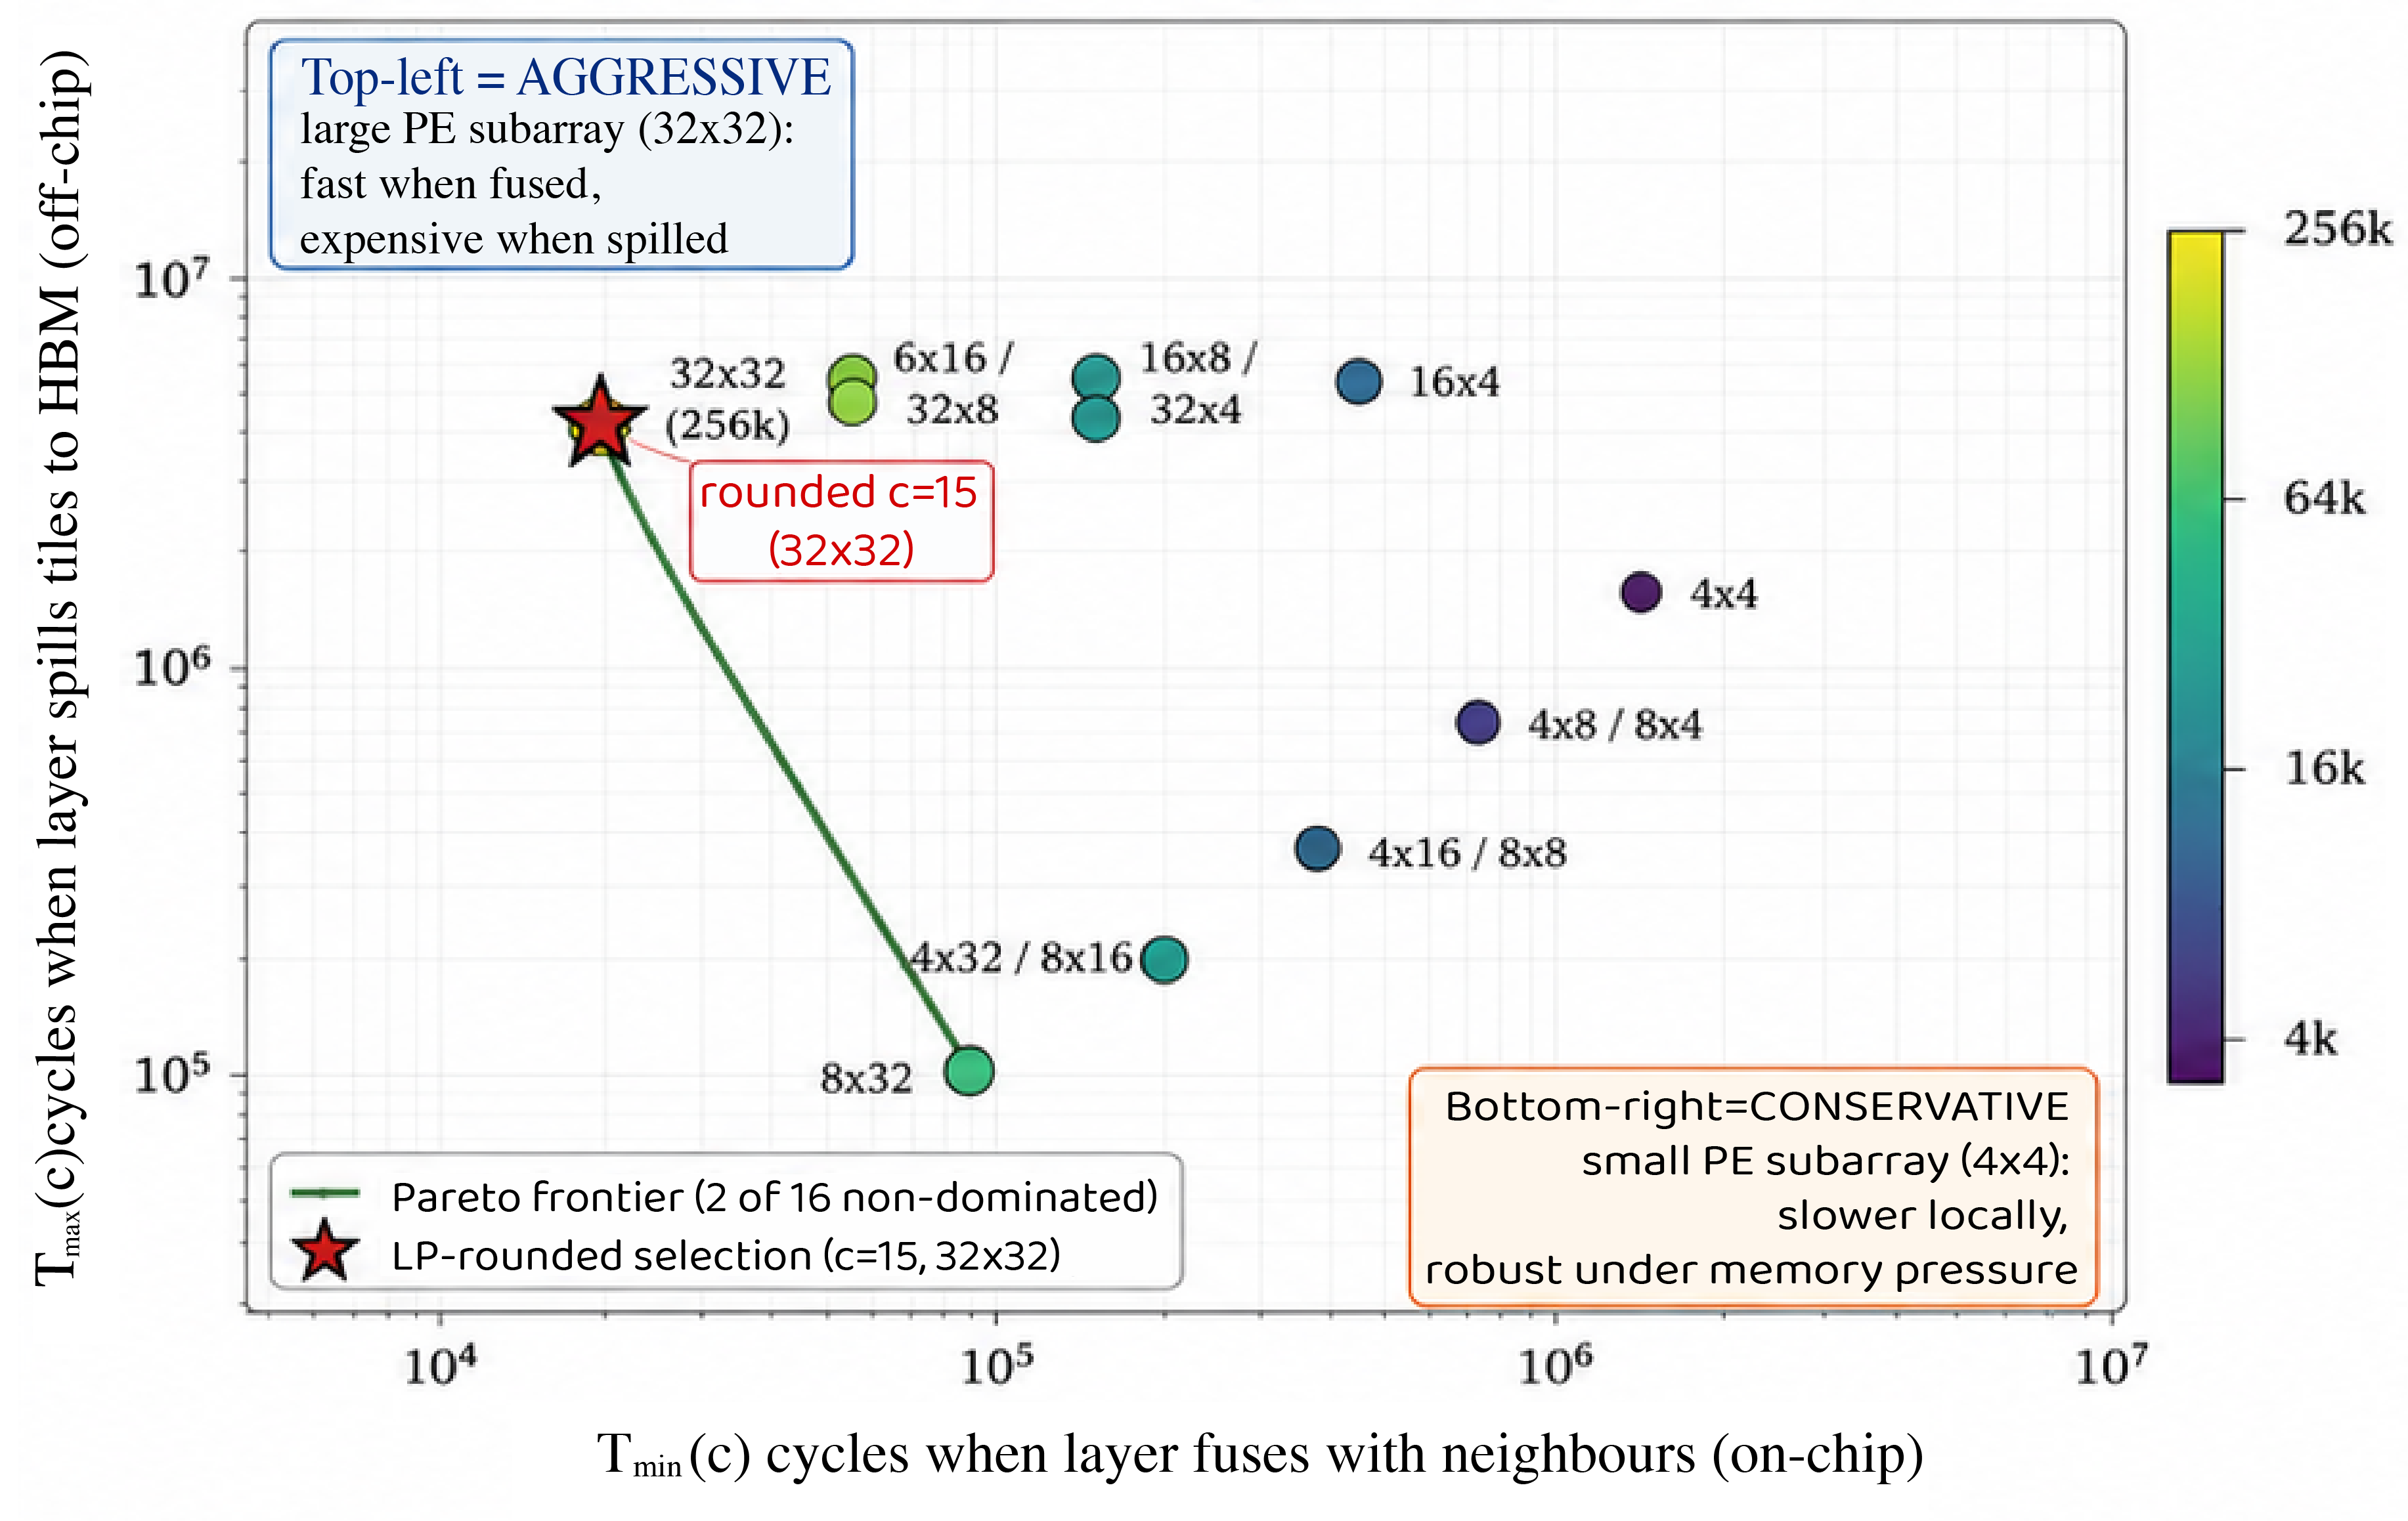
\includegraphics[width=0.48\textwidth]{figs4/pareto_front.png}
\hfill
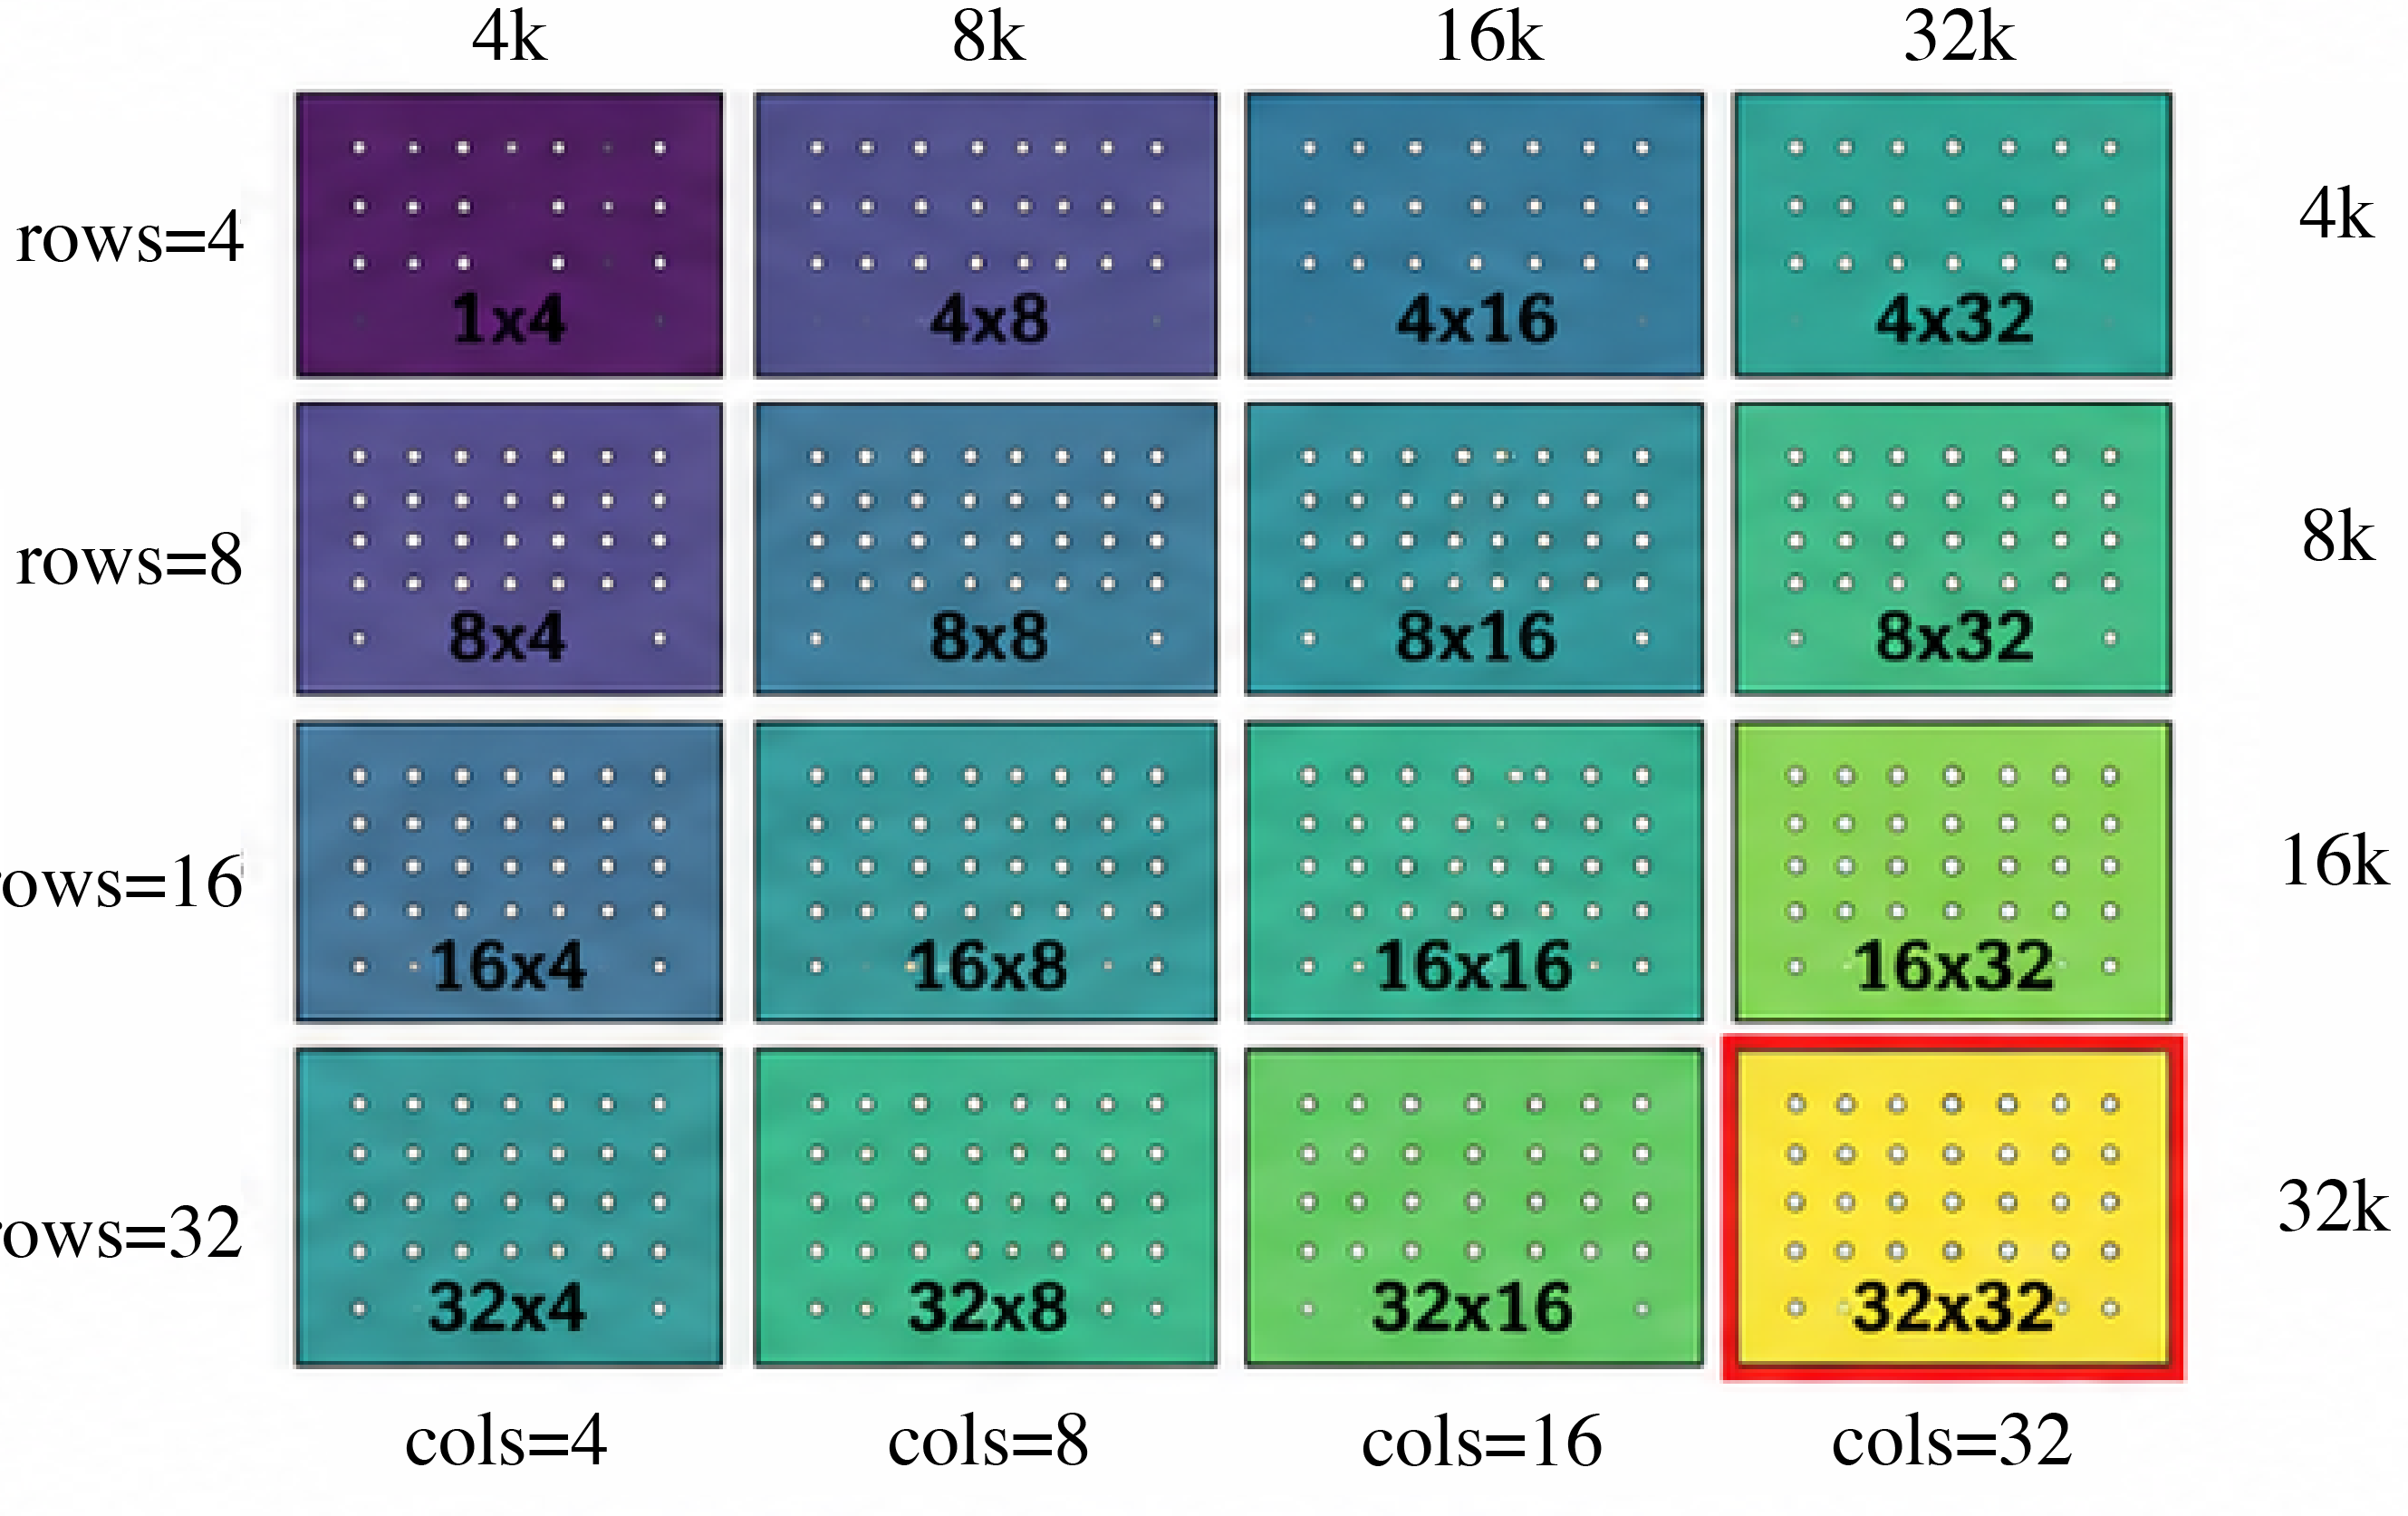
\includegraphics[width=0.48\textwidth]{figs4/tiles.png}
\caption{
Example per-layer tiling cache for EfficientNet-B7 layer L4.
Left: Timeloop-evaluated candidates plotted by fused/on-chip cost
\(T_{\min}(c)\) and spilled/off-chip cost \(T_{\max}(c)\); the frontier shows
non-dominated choices and the star is the LP-rounded selection. Right: the
16 tiling choices; labels such as \(4\times4\),
\(8\times8\), and \(32\times32\) denote active tile rows/columns inside the
fixed accelerator, white dots indicate active PE/MAC sites.
These are schedule choices, not different chips.
}
\label{fig:tiles}
\end{figure}

\paragraph{Per-layer joint candidate tiling advantage.}
For each operation, CHEETAH-V1 precomputes a small set of
Timeloop-evaluated tile mapping configurations and exposes them to the
V1 LP through the selection variables $y_{i,c}$.
Figure~\ref{fig:tiles} illustrates this for one layer: each point is one candidate mapping, with
$T_{\min}(c)$ on the $x$-axis representing the fused/on-chip execution
floor and $T_{\max}(c)$ on the $y$-axis representing the spilled/off-chip cost.
Aggressive mappings (upper left) are fast when fusion succeeds but
expensive, while conservative mappings (lower right) are
slower locally but more robust under memory pressure.
The LP relaxation assigns fractional mass to two configurations in this example,
$y_{15} = 0.71$ and $y_{11} = 0.29$, and the rounded replay selects
$c = 15$ (the $32\times32$ mapping), with only a $3\%$ gap to the LP
lower bound.

This illustrates one core advantage of the CHEETAH-V1 LP: tiling is no
longer fixed before fusion. Instead, tile choice, placement, and
rematerialization are jointly decided, and the solver is free
to choose a locally non-obvious mapping whenever doing so improves the
global schedule. 
Concretely, the V1 LP introduces $y_{i,c}$ alongside
McCormick auxiliary variables $w_{i,c,k}$ to make the tiling selection
interact directly with tensor placement and rematerialization decisions, with Timeloop running once per retained configuration to supply the
triple $\bigl(T_i^{\min}(c),\, T_i^{\max}(c),\, t_i^k(c)\bigr)$ for
each candidate~$c$.
% This demonstrates that by exploiting structural invariance and GPU-accelerated mathematical optimization, CHEETAH-V1 reduces the end-to-end co-design search time from days to under 2.2 hours—a ${\sim}93\%$ average reduction—while discovering architectural points that deliver up to $35\times$ speedup over the TPU-v3 baseline.

% Figure~\ref{fig:pareto} shows the Pareto frontier of best-achieved Perf/TDP versus wall-clock search cost. V1 strictly dominates both V0 and static at every time budget: within 10 minutes of search, V1 already exceeds the best Perf/TDP that V0 or static achieve after 60+ minutes. The V1 Pareto frontier reaches ${\sim}35\times$ Perf/TDP, roughly $3\times$ higher than the V0/static frontier at ${\sim}10\text{--}12\times$. This gap reflects two compounding advantages: V1 explores a strictly larger feasible region (joint tiling-fusion), and it eliminates Timeloop from the per-trial critical path, allowing more trials within any fixed time budget.


\paragraph{LLM Architect vs.\ Optimizer.} Modeled on SkyDiscovery~\citep{skydiscover2026}, the LLM Architect prunes
the outer search loop by proposing campaign patches rather than
predicting raw performance. It analyzes a Causal Ledger containing
invalid rates, MFU, and solver diagnostics to suggest constrained
hardware neighbourhoods for Vizier to explore locally. The V1 LP
remains the ground-truth evaluator, supported by a Roofline Auditor
that rejects physically impossible results.
In a widened search space, the LLM loop reduces invalid evaluations
from $24.5\%$ to $5.9\%$ on average to yield a $4.1\times$ reduction in wasted
trials (Figure~\ref{fig:llm}), while reaching the same optimal Perf/TDP scores as full-space
Vizier. This demonstrates that the LLM's role is steering Bayesian
optimization toward feasible, workload-appropriate subspaces rather than
replacing the solver. We provide exact prompts in Appendix~\ref{app:prompt} for full replication of results, as well as two specific case studies of real-world use cases.
\begin{figure}[ht!]
    \centering
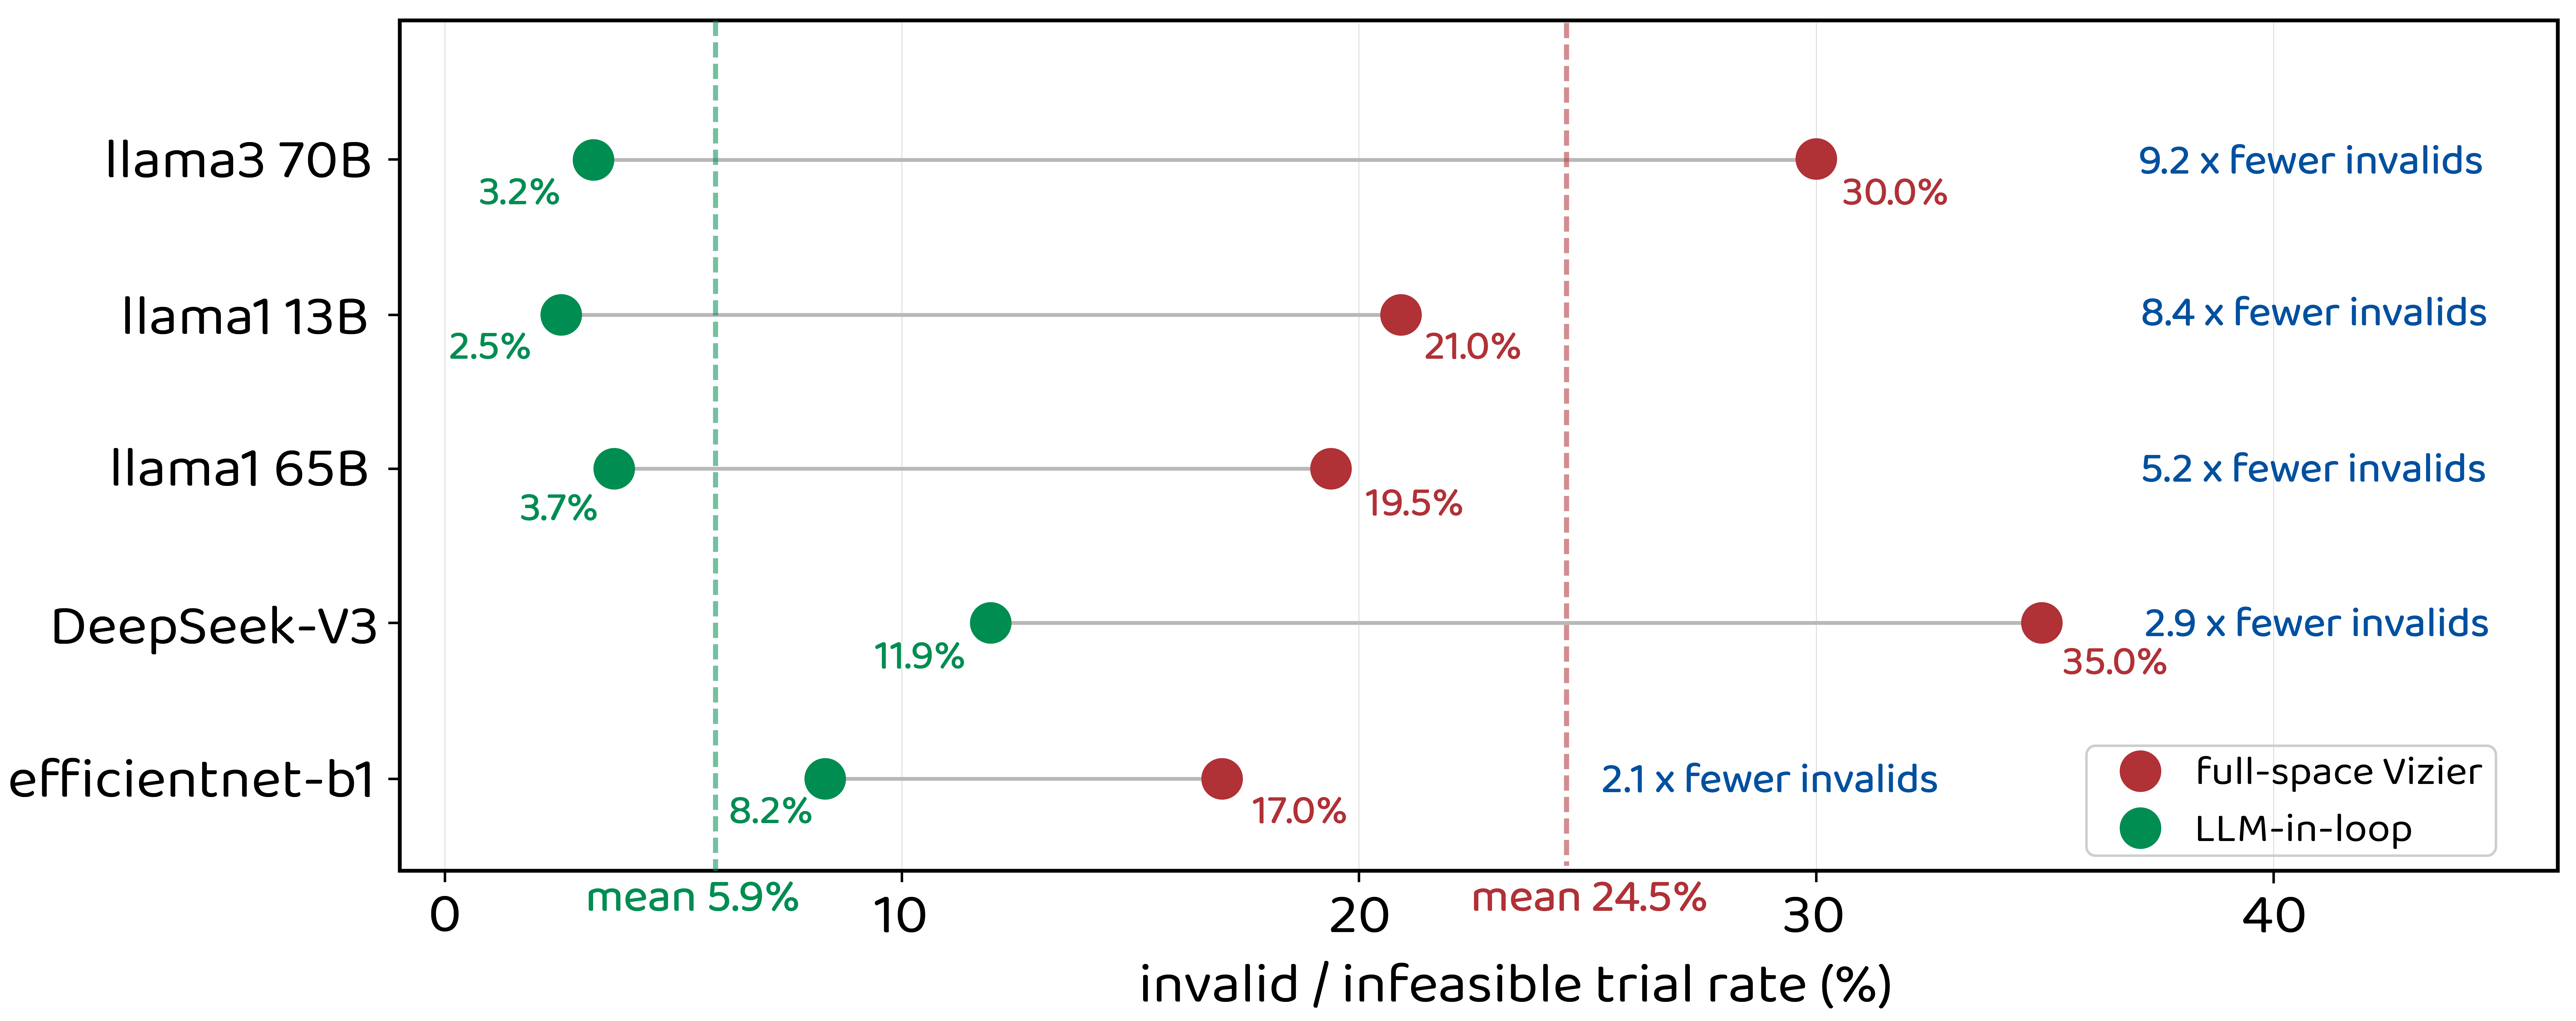
\includegraphics[width=0.85\linewidth]{fig3/llm_guide_v1.png}
\caption{Invalid/infeasible trial rate (\%) for full-space Vizier vs.\ LLM-in-loop across five workloads. The LLM Architect reduces the mean invalid rate from 24.5\% to 5.9\% (4.1$\times$ reduction), with the largest gains on LLM workloads where the hardware search space is most prone to infeasible configurations.}\label{fig:llm}
\end{figure}

% \subsection{Fixed Hardware + Dynamic Planning}


% \section{Conclusion}
% \label{sec:conclusion}

% We present CHEETAH: a co-design framework that combines two powerful LP reformulations with an LLM-Architect guided outer loop to quickly and effectively design custom accelerators. CHEETAH is able to model more global design trade-offs that traditional sequential pipelines cannot unlock, while the outer loop further improves efficiency by steering a hardware configuration tool to suggest positive search neighbors. 
% Our V0 approach extends standard static fusion ILP with time-indexed tensor placement and rematerialization, enabling dynamic memory management within a single inference pass. Our V1 approach further unifies tiling and fusion optimization via McCormick linearization, enabling the solver to discover cross-stage trade-offs that the sequential pipeline systematically misses.
% The joint LP formulation scales to production-size models (2.5M variables, 6.1M nonzeros for DeepSeek-V3) and preserves the structural invariance needed for efficient solver preconditioning across hardware search trials. The largest gains are seen on architectures with diverse layer types where joint tiling-fusion optimization is most impactful.

% % \todo{Add result summary: ``Our experiments demonstrate $X\times$ Perf/TDP improvement over FAST on [workloads], with the largest gains on architectures with diverse layer types where joint tiling-fusion optimization is most impactful.''}

% % \paragraph{Limitations and future work.}
% % % \todo{rooflines and MFU validates, need to run this on a real simulator and finetune}
% % Our current formulation treats the neural network architecture as fixed.
% % A natural extension would co-optimize network architecture, hardware datapath, and compiler decisions in a single framework, building on prior work in hardware-aware NAS.
% % The LP relaxation may produce fractional solutions that require rounding; investigating tighter formulations or branch-and-bound within the LP would improve solution quality.
% % The LLM-guided outer loop is preliminary; a systematic study of prompt engineering, LLM-Vizier integration strategies, and the interaction between LLM reasoning and LP dual information would strengthen this component.
% % Finally, extending the formulation to optimize for training workloads (which require backward-pass memory management and gradient accumulation) is an important direction.

% % \paragraph{Broader impact.}
% % More efficient accelerator design tools can reduce the energy consumption and carbon footprint of datacenter ML inference, which accounts for a growing share of global compute.
% % By lowering the engineering effort and deployment scale required for specialized accelerators to be economically viable, our work may also broaden access to high-performance ML inference beyond the largest technology companies.

% page edit

\section{Conclusion}
\label{sec:conclusion}

% We present CHEETAH, a HW/SW co-design framework that combines two powerful LP reformulations with an LLM Architect guided outer loop to quickly and effectively design custom accelerators. 
We present CHEETAH, a HW/SW co-design framework that combines a strict LP inner loop for physically constrained rules that must not be violated, with an LLM Architect guided outer loop that uses LP duals and trial diagnostics to effectively design high-performance accelerators.
To our knowledge, CHEETAH is the first LP-based inference accelerator co-design framework to jointly optimize tiling, fusion, dynamic placement, scheduling, and rematerialization in one formulation. 
Our framework is composed of two key ideas: LPs excel in solving mathematically modeled problems to proven optimality, and LLMs excel at aggregating vast amounts of information. In this work, we combine these ideas, and delegate the roles in co-design between these two pieces. The division of labor is strict: the solver owns feasibility and the optimality certificate, while the LLM aggregates diagnostics (converged duals, binding constraints, audit verdicts) into search-space interventions. The LLM proposes; the LP certifies. No LLM suggestion can violate a physical constraint, because suggestions only reshape the neighborhood handed to the certified inner problem.
CHEETAH is able to model global design trade-offs that traditional sequential pipelines cannot unlock, while the outer loop further improves efficiency by steering a hardware configuration tool to suggest promising search neighborhoods. 
Our CHEETAH-V0 and CHEETAH-V1 LP reformulations progressively unify placement, rematerialization, and tiling--fusion into a single pass, scaling to 2.5M variables and 6.1M nonzeros on DeepSeek-V3 while preserving the structural invariance needed for efficient solver preconditioning across hardware search trials. The largest gains are seen on architectures with diverse layer types where joint tiling-fusion optimization is most impactful.

This manuscript presents a formal and empirical demonstration that sequential tiling-then-fusion loses solutions, together with a joint optimization method that recovers those solutions in precisely characterized operating regimes.
Sequential accelerator pipelines make locally optimal mapping decisions before they know the global memory schedule; CHEETAH exposes tile choice, tensor residency, and rematerialization to one optimization problem.
We prove that every in-scope sequential map-then-fuse pipeline, lifted FAST included, is contained in CHEETAH's feasible set (Theorem~\ref{thm:containment}), isolate a fixed-hardware free-$y$ gain on Llama-3 70B (2.11$\times$ under every sequential ordering vs.\ 2.51$\times$ for the joint LP), and characterize a second separation regime in capacity-constrained DeepSeek-V3, where tile-dependent footprints admit schedules unavailable to both stock V1 and an oracle two-pass sequential baseline. \todo{DS-V3 capacity-constrained separation not yet measured at a harsher CGM point (2--4\,MiB, activations binding); max measured so far is 0.077\% at CGM$=$4\,MiB. Run before release or soften this clause.}

In sum, the paper contributes a new mathematical abstraction for global HW/SW co-design; an exact cross-stage tradeoff that FAST cannot express; a rounded, simulator-replayed validation proving the gains are not just an LP artifact; a decomposition of how the $40\times$ arises; and sensitivity sweeps showing it is not just more MACs.
All utilization quantities we report are roofline-model diagnostics, not measured silicon utilization; real implementations would still incur NoC, SRAM, pipeline, and control overheads.

Future work can build from this framework in two meaningful ways: as an end-to-end co-design system for efficient accelerators, and as an automated optimization engine for existing hardware. By fixing the architecture, the inner loop derives optimal tiling and scheduling strategies that can act as custom speedups for targeted inference tasks.

\section{Submission of papers to NeurIPS 2026}



\begin{itemize}
    \item Older GPUs had ridgepoints around 5–10 $FLOPs/Byte$. Now accelerators have ridgepoints above 100–200 $FLOPs/Byte$. This means modern chips are computationally rich but starved for data, making them much harder to fully utilize unless we have very high data reuse (like large matrix multiplications).
    \item Example from FAST paper : EfficientNet on TPU-v3. Depthwise convolutions utilize about 9 out of 128 slots in a 128×128 systolic array = wasteful. FAST finds that a 32×32 systolic array is actually much better for this workload because it fits the problem dimensions better, even though it sounds "smaller." No human engineer would have looked at this combination systematically.
    \item there is Tension between what LLMs can do and what should be rigorously formulated and calculated in a principled mathematical, way, we want to balance this tension to get the best of both worlds

\end{itemize}


%%%%%%%%%%%%%%%%%%%%%%%%%%%%%%%%%%%%%%%%%%%%%%%%%%%%%%%%%%%%

\appendix

\section{Technical appendices and supplementary material}

%%%%%%%%%%%%%%%%%%%%%%%%%%%%%%%%%%%%%%%%%%%%%%%%%%%%%%%%%%%%

\section{LP Matrix Structure Analysis}


\begin{table}[h]
\centering
\begin{tabular}{lll}
\toprule
\textbf{Feature} & \textbf{Depends On} \\
\midrule
$m, n$ (rows, cols) & $L$ (layer count), $C$ (Pareto count), $T$ (timesteps) \\
$\text{nnz}$ (number of nonzeros) & LP formulation structure \\
Sparsity pattern & Constraint topology \\
Block structure & LP variable grouping \\
eq/ineq ratio & Constraint types \\
Numerical values in $A, c, l_c, u_c$ & Timeloop cycle counts ($T_{\max}$, $t_W$, etc.)\\
\bottomrule
\end{tabular}
\caption{LP matrix dependence and what changes with Vizier per hardware reference data.}
\end{table}


Only the numerical coefficients change but the matrix shape is identical across the same method:
\begin{itemize}
    \item $A_{\text{data}}$ values change (rescaled by BW (bandwidth), GLB (global buffer), etc.)
    \item $c$ values change (objective weights)
    \item $l_c$, $u_c$ values change (constraint bounds)
    \item $A_{\text{indices}}$, $A_{\text{shape}}$ stay identical
\end{itemize}

\subsection{Formulation Structure for 3 Methods: original static, v0, v1}

\paragraph{Static FAST ILP.}
For each NN model the sparsity pattern is fixed:
\begin{itemize}
    \item $4L$ variables: $\bigl[T_i\ (L),\ p^I\ (L),\ p^O\ (L),\ p^W\ (L)\bigr]$
    \item ${\sim}3L$ constraints with $L{+}1$ nonzeros per row
    \item Block layout: dense bottom-right ``$T_i$ + pinning'' block
\end{itemize}

\paragraph{V0 Dynamic LP.}
Block time indexed structure with remat:
\begin{itemize}
    \item $L + 4LT$ variables
    \item $L \times T$ constraint blocks repeating (memory capacity per
          timestep, persistence per timestep, weight monotone, remat)
    \item The block-banded structure is identical per model across all
          hardware proposals and only coefficient magnitudes change with HW
\end{itemize}

\paragraph{V1 Joint Tiling LP.}
McCormick envelope bilinear matrix structure:
\begin{itemize}
    \item $L + LC + ET + LT + LT + 3LC$ variables
    \item Four distinct constraint blocks:
          assignment, McCormick linearization, capacity, persistence
    \item $C = 10$ Pareto configs always (set by \texttt{C\_PARETO} constant)
    \item Same sparsity pattern per model
\end{itemize}

\subsection{Implications for Preconditioner Design}

Three preconditioners can be designed (one per formulation category)
based on the current matrices.
They will generalize to any hardware reference data, and should generalize for any NN model as well:

\begin{enumerate}
    \item \textbf{Static preconditioner} — designed for the dense
          $L \times L$ pinning block; scales with $L$ across all 13 model
          sizes.

    \item \textbf{V0 preconditioner} — designed for the $L \times T$
          block-banded structure; works regardless of which hardware Vizier
          proposes, since block sizes and locations are invariant to HW
          coefficients.

    \item \textbf{V1 preconditioner} — designed for the McCormick envelope
          between the $y_{i,c}$, $p_{e,t}$, and $w_{i,c,k}$ blocks;
          structurally invariant per model.
\end{enumerate}

The only things that change across models within the same category are
$L$, $C$, and $T$: but these scale the existing block pattern without
changing its topology.
The preconditioner can therefore be made \emph{parametric} in $(L, C, T)$
rather than hardcoded, and will generalize across all 13 models and any
future Vizier-proposed hardware configurations.

\begin{remark}
    Changing \texttt{C\_PARETO} (currently $C = 10$) will alter the V1
    variable count and break preconditioner reuse.
    Specifically, the McCormick block dimensions scale as $L \times C \times 3$,
    so bumping to $C = 20$ or $C = 50$ shifts the V1 matrix structure.
    Keep \texttt{C\_PARETO} constant if preconditioner portability across
    hardware proposals is required. Unless CORGI is robust enough at point of submission, then we can look at increasing C. 
\end{remark}

\begin{table}[h!]
\centering
\begin{tabular}{>{\ttfamily}l p{8cm}}
\toprule
\normalfont\textbf{Parameter} & \textbf{Description} \\
\midrule
PEs\_x\_dim, PEs\_y\_dim        & How many PEs in the grid (4$\times$4? 8$\times$8? 64$\times$64?) \\[4pt]
systolic\_array\_x/y            & How big is each PE's systolic array \\[4pt]
vector\_unit\_multiplier        & How wide is the vector unit in each PE \\[4pt]
L1\_buffer\_config              & Does each PE get its own L1, or share one? \\[4pt]
L1\_input/weight/output\_size   & How big is L1 memory \\[4pt]
L2\_buffer\_config              & Does L2 exist at all? \\[4pt]
L3\_global\_buffer\_size        & How big is the on-chip global buffer \\[4pt]
GDDR6\_channels                 & How many wires connect to off-chip DRAM \\[4pt]
native\_batch\_size             & How many inputs processed simultaneously \\
\bottomrule
\end{tabular}
\caption{Hardware design space parameters}
\end{table}

\bigskip

Each combination of these numbers describes a completely different physical chip.
A chip with 64 PEs each containing a $32 \times 32$ systolic array looks and behaves
completely differently from a chip with 8 PEs each containing a $128 \times 128$
systolic array, even if their raw TFLOPS numbers are similar on paper. What we actually use: MAC range: 256 (Edge TPU) - 1M (H100-class)
BW range: 64–512 GB/s, with roofline coupling for V1
CGM range: 1–16 MB, floored per-model for feasibility
Quadratic TDP penalty above TPU-v3 MACs rules out oversized chips
Roofline cap in V1 rescaling rules out "tiny chip + huge BW" cheat code

\mnote{Where V1 shows its strength the most. Listed from most impact to least impact: } Architectures have very diverse layer types with different memory-compute tradeoffs, where choosing the right tile size per operation unlocks fusion that a fixed tiling can't.

- MobileNetV3 / MobileNetV4 (Google, 2019/2024)

Same depthwise-separable + squeeze-excite structure as EfficientNet but with h-swish activations and neural architecture search (NAS) blocks. Depthwise layers have tiny weights but huge activations, pointwise layers are the opposite. Fixed tiling can't serve both.
Very popular for on-device inference (phones, edge TPUs)

- EfficientViT / EfficientFormer (MIT/Snap, 2023)

Hybrid CNN-transformer: depthwise convolutions + linear attention. Two fundamentally different layer types in the same model — depthwise (memory-bound, low OpInt) and attention matmuls (compute-bound at long sequences). V1 can pick different tiles for conv blocks vs attention blocks. Static/V0 can't.


- ConvNeXt V2 (Meta, 2023)

Modernized ResNet with depthwise 7×7 convolutions + LayerNorm + GELU
Large kernel depthwise creates huge activation working sets (7×7 vs 3×3). V1's per-op tiling handles the large-kernel layers better than a global tile choice.

- Mixtral / Mixture-of-Experts (MoE) (Mistral, 2024)

Each token routes to 2 of 8 expert FFN blocks, creating variable per-layer memory footprint
At inference, only 2 experts are active but all 8 sets of weights must be accessible
V1 can tile the active experts differently from the routing/attention layers. V0's remat also helps here: evict inactive expert weights, remat if re-activated

- Mamba / State Space Models (Gu and Dao, 2024)

No attention — uses selective scan (sequential recurrence) instead. Very different compute pattern: scan operations are sequential (low parallelism), projections are standard matmuls (high parallelism). V1 can select tiling that maximizes GLB utilization during the sequential scan phases while using aggressive tiling during projections. Growing in popularity as attention-free alternative
Stable Diffusion / U-Net backbone (Stability AI, 2022-2024)

- Llama 3.1 / Qwen2 / DeepSeek-V3 (GQA + SwiGLU)

You already have Llama, but newer variants have larger FFN ratios (DeepSeek-V3: FFN dim = 18,432 for 7B params)
Larger FFN → bigger weight matrices → more memory pressure → V1's tiling helps more

- Vision Transformers (ViT, DINOv2)

Patch embedding (conv) + transformer blocks
Less diverse than EfficientNet but V1 still helps at high resolution (large activation tensors)
Why these architectures specifically
The pattern is: V1 gains are largest when the model has Mixed layer types (depthwise + pointwise + attention + scan) — one tile size can't serve all
Large activation-to-weight ratio — forces fusion/eviction decisions
Skip connections or multi-fanout — tensors must stay alive across multiple consumers
Memory-bound operational intensity (OpInt < 100 FLOPS/B) — DRAM traffic dominates, fusion is the primary optimization lever


\mnote{When v0 shows its strength the most:Memory pressure is tight, dependency chains are long, per-layer costs change dramatically.}

- DeepSeek-V3 (671B, MoE) at batch=1

256 experts × FFN, only 2 active per token → active weight count changes per step
V0's time-indexed placement: pin only the active experts each step
V0's remat: recompute a cheap expert output vs reload 44 GB of expert weights
Expected V0 gain: 40-60\% vs static


- Llama 3.1 / 3.3 405B at 128K context

KV cache at long context exceeds HBM capacity → must evict mid-run
Remat cheap attention layers vs reload 800 GB weights
Demonstrates V0's core value: memory pressure over time
Expected V0 gain: 30-50\% vs static


- Mamba-2 / Jamba (hybrid state-space)

Sequential scan creates unique dependency chains
Scan state is evict-then-remat ideal
Very different from transformer access pattern — compelling novelty
Expected V0 gain: 25-40%

- Qwen2.5-72B / DeepSeek-R1 at inference

Long-context reasoning models with massive KV caches
Remat dominates: recomputing tokens is cheap, KV reload is expensive
Expected V0 gain: 20-35\%
Tier 1 — Maximum V1 (joint tiling + fusion) gains

\mnote{V1 wins when: layer types are diverse, working-set sizes vary by 100×+, fusion requires tile flexibility.}

- Flux.1 / Stable Diffusion 3.5 (diffusion transformer)

Mixed CNN backbone + multi-resolution transformer + cross-attention
U-Net skip connections → tensor lifetime spans entire network (V1's edge-indexed $p_{e,t}$ shines)
20-50 denoising steps per image → fusion across steps
Expected V1 gain: 30-50\% vs V0
Commercially relevant: image generation dominates GPU hours at OpenAI/Google


- DeepSeek-V3 MoE (also V1 winner)

Router + attention + 256 experts all want different tiles
V1's $y_{i,c}$ tiling selection is mathematically natural for MoE's "which expert" routing
Novel angle: joint tiling + joint expert selection
Expected V1 gain: 30-45% vs V0
Segment Anything Model 2 (SAM 2) (image encoder + lightweight decoder)

Extreme layer diversity: huge ViT encoder (~ViT-Huge) + tiny mask decoder (~3 layers)
No single tile size fits both
Expected V1 gain: 40-60\% vs V0


- EfficientViT / FastViT / MobileNetV4 (hybrid CNN-transformer at edge)

Depthwise conv + linear attention + SE blocks + FFN in one model
Tile sizes differ by 100× between layers
Expected V1 gain: 25-40%
Edge-relevant: showcases V1 for mobile/embedded accelerators
RWKV v6 / v7 (linear transformer alternative)

Mixed matrix shapes, time-mixing vs channel-mixing layers
Compelling because it's an attention alternative gaining traction
Expected V1 gain: 20-35\%
\newpage
%\input{checklist.tex}
\mnote{Key insight of V1 is  the pareto front shape is bandwidth invariant:} precompute Pareto configs once, rescale per trial, therefore we can pull the time intensive Timeloop out of the entire loop


\end{document}